%% METIS_DRLD.tex
%%
%% METIS data reduction library design document
%%
%% 2020-05-27: initialised from specification document (OC)
%% 2020-09-07: MTR release (OC)
%% 2202-07-01: v0.4 Internal Review (HB)

\newcommand{\doctitle}{%
  \parbox[t]{\textwidth}{Data Reduction Library\\Design}}
\newcommand{\docnumber}	{E-REP-AST-MET-1006}     % Document number
%% Email from Sander: "... set them all to issue 1-0 and only include update dates in the changelog.
\newcommand{\issuenumber}{1-0}                % Version
\newcommand{\issuedate}{2023-08-08}              % Date
\newcommand{\workpackage}{8.2}      % Workpackage

% The purpose of texorpdfstring is to provide different
% strings for the title page (tex string) and for the pdf bookmark
% (via hyperref, no tex formatting allowed).
% The two versions need to be kept in sync.
\newcommand{\authorname}{\texorpdfstring{%  % Authors
  H.~Buddelmeijer,\\                        % tex string
  W.~Kausch,\\
  O.~Czoske,\\
  N.~Sabha,\\
  J.~Karr,\\
  C.-H.~Yan,\\
  T.~Marquart,\\
  G.~Otten,\\
  M.~Baláž,\\
  K.~Leschinski,\\
  W.~Zeilinger}
  {Buddelmeijer, Kausch, Czoske, Sabha, Karr, Yan, Marquart, Otten, Baláž, Leschinski, Zeilinger}  % pdf string
  }

\newcommand{\authorsigndate}  {} % date of signature of author

\newcommand{\reviewername}     {%
}       % checked by name
\newcommand{\reviewersigndate} {} % date of signature of checker

\newcommand{\approvername}    {%
}       % name of the approver
\newcommand{\approvalsigndate}{} % date of signature of approver

\newcommand{\releasername}{%
}
\newcommand{\releasesigndate}{}  % date of release

% Title displayed in the header
\newcommand{\shorttitle}{Data Reduction Library Design}


\newcommand{\aj}{The Astronomical Journal}
\newcommand{\aap}{Astronomy \& Astrophysics}
\newcommand{\aaps}{Astronomy \& Astrophysics, Supplement}
\newcommand{\mnras}{Monthly Notices of the Royal Astronomical Society}
\newcommand{\procspie}{Proceedings of the International Society for Optical Engineering}
\newcommand{\pasp}{Publications of the Astronomical Society of the Pacific}
\newcommand{\apjs}{The Astrophysical Journal, Supplement}


%%%%%%%%%%%%%%%%%%%%%%%%%%%%%%%%%%%%%%%%%%%%%%%%%%%%%%%%%%%%%%%%%%%%%%%%%%%%%
\documentclass[11pt,oneside,a4paper]{article}

%% Layout  --- TeX commands
\raggedbottom
\topmargin=-9mm
\headsep=0.5cm
\textheight=246mm
\textwidth=164mm
\hoffset=0cm
\oddsidemargin=-2mm
\parindent=0mm
\parskip=0.3em

\renewcommand{\floatpagefraction}{0.98} % separate float page does not work
\renewcommand{\bottomfraction}{1.0}

%% Fonts
\usepackage{mathptmx}
\usepackage[scaled=0.92]{helvet}

\usepackage[pdftex]{graphicx}
\graphicspath{{./figures/}}
\makeatletter
\def\input@path{{./}{./tikz/}}
\makeatother

\usepackage{siunitx}
\usepackage{fancyhdr}
\setlength{\headheight}{19pt} % ...at least 18.26802pt
\setlength{\footskip}{31pt}   % ...at least 30.86163pt
\usepackage{titlesec}
\usepackage{booktabs}
\usepackage{tabularx}
\usepackage{array}
\usepackage{longtable}
\usepackage{numprint}
\usepackage{placeins}
\usepackage{enumitem}
\usepackage{acronym}
\usepackage[dvipsnames]{xcolor}
\usepackage{xcolor}
\usepackage{colortbl}
\definecolor{listingbg}{gray}{0.95}
\definecolor{darkgreen}{rgb}{0.0, 0.7, 0.0}
\definecolor{darkblue} {rgb}{0.0, 0.0, 0.7}
\definecolor{darkred}  {rgb}{0.7, 0.0, 0.0}
\definecolor{darkorange}{rgb}{1.0, 0.49, 0.0}

\usepackage{tikz}
\usepackage[many]{tcolorbox}
\usepackage{multirow}

%%% This file contains definitions of shapes and nodes used
%%% for a recipe workflow
%%% Author       : Oliver Czoske
%%% Created      : 2021-03-03
%%% Last Changed : 2021-03-03
%%% Changes:
%%%

\usetikzlibrary{
  shapes.misc,
  positioning,
  calc,
  arrows.meta}

%% All connecting lines have an arrow
\tikzset{
  connection_arrow/.style={->, >=Latex[open], thick}
}

%% Start and stop buttons (black disks, stop with ring)
%% These are pics, use as
%%         \pic (name) [above of=..] {picname};
\tikzset{
  start/.pic = {
    \node (-m) at (0, 0){};
    \filldraw [fill=black] (0, 0) circle (0.2);
  }
}

\tikzset{
  stop/.pic = {
    \node (-m) at (0, 0){};
    \node (-t) at (0, -0.3){};
    \filldraw [fill=black] (0, 0) circle(0.2);
    \draw[black] (0, 0) circle (0.3);
  }
}


%%%% Various boxes and their colours
%%%% These are nodes, use as
%%%% \node (name) [type, location]  {text};

\definecolor{stepcolor}{RGB}{210,169,188}
\definecolor{rawcolor}{RGB}{205,205,205}
\definecolor{externalcolor}{RGB}{183,255,255}
\definecolor{calibcolor}{RGB}{255,250,216}
\definecolor{calproductcolor}{RGB}{185,184,237}
\definecolor{qcproductcolor}{RGB}{255,201,165}
\definecolor{sciproductcolor}{RGB}{197,219,183}
\definecolor{framecolor}{RGB}{127,13,65}

\tikzset{
  %% template : the template(s) that trigger(s) the recipe
  template/.style={
    rectangle,
    draw=black,
    minimum width=4.0cm,
    minimum height=0.5cm,
    align=center
  },
  %% input : the input files
  input/.style={
    rectangle,
    fill=rawcolor,
    minimum width=4.0cm,
    minimum height=0.75cm,
%     text width=3cm,
    align=center
  },
  %% calib : calibration input
  calib/.style={
    rectangle,
    fill=calibcolor,
    minimum width=4.0cm,
    minimum height=0.75cm,
%     text width=3cm,
    align=center
  },
  %% external : external input
  external/.style={
    rectangle,
    fill=externalcolor,
    minimum width=4.0cm,
    minimum height=0.75cm,
%     text width=3.5cm,
    align=center
  },
  %% params : parameters
  params/.style={
    rectangle,
    draw=red,
    thick,
    minimum width=4.0cm,
    minimum height=0.75cm,
%     text width=3cm,
    align=center
  },
  %% redstep : a reduction step
  %%      ("step" is predefined and can't be used)
  redstep/.style={
    rectangle,
    rounded corners=0.2cm,
    fill=stepcolor,   %%% define colour!
    minimum width=4.0cm,
    minimum height=1cm,
%     text width=3cm,
    align=center
  },
  %% connection : connection to input or output
  connection/.style={
    circle,
    fill=black,
    minimum size=0.15cm,
    inner sep=0pt
  },
  %% sciproduct : a science product
  sciproduct/.style={
    rectangle,
    fill=sciproductcolor,
    minimum width=4.0cm,
    minimum height=0.75cm,
%     text width=3.5cm,
    align=center
  },
  %% calproduct : a calibration product
  calproduct/.style={
    rectangle,
    fill=calproductcolor,
    minimum width=4.0cm,
    minimum height=0.75cm,
%     text width=3.5cm,
    align=center
  },
  %% frame : frame around the recipe
  %% This is a path, use as
  %%    \draw [frame] (upper left) rectangle (lower right);
  frame/.style={framecolor, very thick, dashed}
}


% does not work with my version of biblatex:
% \usepackage[defernumbers=true,backend=biber,hyperref=true,url=false]{biblatex}
\usepackage[%
   defernumbers=true,
   backend=biber,
   hyperref=true,
   url=false,
   sorting=none]{biblatex}

\usepackage[%
% pagebackref=true,   % does not work with biblatex
   pdfpagelabels=true,
   plainpages=false,
   colorlinks=false]{hyperref}


% Git stuff, must by after hyperref
% The git hash and commit date will be shown when compiling with --shell-escape
% https://tex.stackexchange.com/a/598669/2775
\newif\ifshowgit  % flag to show git info instead of Issue info
% "The control sequence \pdfshellescape is (only?) available in pdftex"
% http://tex.stackexchange.com/a/13253/2595
\ifnum\pdfshellescape=1{ %
    % Check for overleaf https://tex.stackexchange.com/a/598669/2775
    \ifnum\pdfstrcmp{\jobname}{output}=0
        % Apparently overleaf does not compile from their git repo.
        \showgitfalse
    \else
        \usepackage[noheader]{gitver}
        \def\parsegitdate#1-#2-#3 #4\endparse{#3.#2.#1}
        \makeatletter
            \edef\gitdate{\@@input|"git log -1 --format=\@percentchar ci"}
        \makeatother
        \showgittrue
    \fi
\else
    \showgitfalse
\fi


% does not work with my version:
%\usepackage[xindy,nopostdot,nogroupskip]{glossaries}
\usepackage[xindy]{glossaries}
%\makeglossaries

\usepackage{lastpage}
\usepackage{multirow}
\usepackage[%
   font=small,
   format=plain,
   indention=1.5em,
   labelfont={small,bf},
   up,
   justification=justified,
   singlelinecheck=true]{caption}

%% for sidewaysfigure and sidewaystable
\usepackage{rotating}

%% for landscape
\usepackage{pdflscape}

% for newgeometry and restoregeometry
\usepackage{geometry}

%% put recipe names, QC parameters, etc., in \lstinline{}
\usepackage{listings}
\lstloadlanguages{csh, c}

\usepackage{textcomp}

\usepackage{csquotes}

\usepackage[countmax]{subfloat}

%\setcounter{tocdepth}{4}
\setcounter{secnumdepth}{4}


% ADDING NEW DEFINITIONS -------------------------------------------- start

% ADDING NEW DEFINITIONS -------------------------------------------- start
\definecolor{listingbg}{gray}{0.95}
\definecolor{darkgreen}{rgb}{0.0, 0.7, 0.0}
\definecolor{darkblue} {rgb}{0.0, 0.0, 0.7}
\definecolor{cyan} {rgb}{0.0, 0.4, 0.4}
\definecolor{darkred}  {rgb}{0.7, 0.0, 0.0}
\definecolor{darkorange}{rgb}{1.0, 0.49, 0.0}
\definecolor{violet}{rgb}{255, 0, 255}
\definecolor{turq}{rgb}{0.0, 0.7, 0.8}
\definecolor{fits}{rgb}{0.4, 0.1, 1}


\makeatletter
\lstdefinestyle{RAWstyle}{%
  basicstyle=\ttfamily\color{fits}%
  \lst@ifdisplaystyle\scriptsize\fi}

\lstdefinestyle{PARstyle}{%
  basicstyle=\ttfamily\color{cyan}%
  \lst@ifdisplaystyle\scriptsize\fi}

\lstdefinestyle{DRLstyle}{%
  basicstyle=\ttfamily\color{violet}%
  \lst@ifdisplaystyle\scriptsize\fi}

\lstdefinestyle{RECstyle}{%
  basicstyle=\ttfamily\color{darkgreen}%
  \lst@ifdisplaystyle\scriptsize\fi}

%% Write QC parameters like this: \QC{QC_SOMETHING_OR_OTHER}
\lstdefinestyle{QCstyle}{%
  basicstyle=\ttfamily\color{darkblue}%
  \lst@ifdisplaystyle\scriptsize\fi}

%% Write templates like this: \TPL{DARK_LM}
\lstdefinestyle{TPLstyle}{%
  basicstyle=\ttfamily\color{darkred}%
  \lst@ifdisplaystyle\scriptsize\fi}

%% Write products like this: \hyperref[dataitem:some_thing]{\PROD{SOME_THING}}
\lstdefinestyle{PRODstyle}{%
  basicstyle=\ttfamily\color{darkorange}%
  \lst@ifdisplaystyle\scriptsize\fi}

%% external calib files
\lstdefinestyle{EXTCALIBstyle}{%
  basicstyle=\ttfamily\color{Turquoise}%
  \lst@ifdisplaystyle\scriptsize\fi}

% static calib files
\lstdefinestyle{STATCALIBstyle}{%
  basicstyle=\ttfamily\color{teal}%
  \lst@ifdisplaystyle\scriptsize\fi}
\makeatother


\makeatletter
\newcommand{\replaceunderscores}[1]{\expandafter\replace@underscores#1_\relax}

\def\replace@underscores#1_#2\relax{%
    \ifx \relax #2\relax
        #1%
    \else
        #1%
        \textunderscore
        \replace@underscores#2\relax
    \fi
}

\ExplSyntaxOn
% Generic \Smart@Item macro:
%   use \NEWRAW*{WHATEVER_THIS_IS} where hyperlinks are not needed (TOC, sections...)
%   and \NEWRAW{WHATEVER_THIS_IS} for a full hyperlink-enabled version in regular text and tikz figures
\NewDocumentCommand{\Smart@Item}{m m m O{dataitem}}{%
    \IfBooleanTF{#1}{%
        \texorpdfstring{\lstinline[style=#2style]!#3!}{\replaceunderscores{#3}}%
    }{%
        \hyperref[#4:\text_lowercase:n{#3}]{\lstinline[style=#2style]!#3!}%
    }%
}
\ExplSyntaxOff

% Raw FITS file: \NEWRAW{LM_SCI_RAW}
\NewDocumentCommand{\NEWRAW}{s m}{\Smart@Item{#1}{RAW}{#2}}
\NewDocumentCommand{\NEWPAR}{s m}{\Smart@Item{#1}{PAR}{#2}}
\NewDocumentCommand{\NEWDRL}{s m}{\Smart@Item{#1}{DRL}{#2}}
\NewDocumentCommand{\NEWREC}{s m}{\Smart@Item{#1}{REC}{#2}[rec]}
\NewDocumentCommand{\NEWQC}{s m}{\Smart@Item{#1}{QC}{#2}}
\NewDocumentCommand{\NEWTPL}{s m}{\Smart@Item{#1}{TPL}{#2}}
\NewDocumentCommand{\NEWPROD}{s m}{\Smart@Item{#1}{PROD}{#2}}
\NewDocumentCommand{\NEWREQ}{s m}{\Smart@Item{#1}{REQ}{#2}}
\NewDocumentCommand{\NEWEXTCALIB}{s m}{\Smart@Item{#1}{EXTCALIB}{#2}}
\NewDocumentCommand{\NEWSTATCALIB}{s m}{\Smart@Item{#1}{STATCALIB}{#2}}
\NewDocumentCommand{\NEWFITS}{s m}{\Smart@Item{#1}{FITS}{#2}}
\makeatother

%% Write DRL functions names like this: \hyperref[drl:function]{\DRL{function}}
\newcommand{\RAW}[1]{ \texorpdfstring{\lstinline[style=RAWstyle]!#1!}%
                                     {\replaceunderscores{#1}}}

%% Write DRL functions names like this: \hyperref[drl:function]{\DRL{function}}
\newcommand{\PAR}[1]{ \texorpdfstring{\lstinline[style=PARstyle]!#1!}%
                                     {\replaceunderscores{#1}}}

%% Write DRL functions names like this: \hyperref[drl:function]{\DRL{function}}
\newcommand{\DRL}[1]{ \texorpdfstring{\lstinline[style=DRLstyle]!#1!}%
                                     {\replaceunderscores{#1}}}

%% Write recipe names like this: \REC{metis_do_stuff}
\newcommand{\REC}[1]{ \texorpdfstring{\lstinline[style=RECstyle]!#1!}%
                                     {\replaceunderscores{#1}}}

%% Write QC parameters like this: \QC{QC_SOMETHING_OR_OTHER}
\newcommand{\QC}[1]{ \texorpdfstring{\lstinline[style=QCstyle]!#1!}%
                                    {\replaceunderscores{#1}}}

%% Write templates like this: \TPL{DARK_LM}
\newcommand{\TPL}[1]{ \texorpdfstring{\lstinline[style=TPLstyle]!#1!}%
                                     {\replaceunderscores{#1}}}

%% Write products like this: \hyperref[dataitem:some_thing]{\PROD{SOME_THING}}
\newcommand{\PROD}[1]{ \texorpdfstring{\lstinline[style=PRODstyle]!#1!}%
                                      {\replaceunderscores{#1}}}

%% Write requirements like this: \REQ{METIS-xxxx}
\newcommand{\REQ}[1]{\href{https://polarion.astron.nl/polarion/\#/project/METIS/workitem?id=#1}{\textcolor{brown}{#1}}}

%% external calib files
\newcommand{\EXTCALIB}[1]{ \texorpdfstring{\lstinline[style=EXTCALIBstyle]!#1!}%
                                          {\replaceunderscores{#1}}}

% static calib files
\newcommand{\STATCALIB}[1]{ \texorpdfstring{\lstinline[style=STATCALIBstyle]!#1!}%
                                           {\replaceunderscores{#1}}}

%% Write FITS keywords (and values) like this: \FITS{EXPTIME}
\newcommand{\FITS}[1]{ \texorpdfstring{\lstinline[]!#1!}%
                                      {\replaceunderscores{#1}}}


\usetikzlibrary{shapes.geometric}
\usetikzlibrary{arrows.meta, arrows.spaced}
\usetikzlibrary{shapes.misc, positioning}
\usetikzlibrary{fit,backgrounds}
\usetikzlibrary{external}
\usetikzlibrary{calc}
%\tikzexternalize % activate!

%% Color definitions
\definecolor{recipecolor}{RGB}{210,169, 188}
\definecolor{rawcolor}{RGB}{235,235,235}
\definecolor{externalcolor}{RGB}{183,255,255}
\definecolor{calibcolor}{RGB}{255,250,216}
\definecolor{calproductcolor}{RGB}{185,184,237}
\definecolor{qcproductcolor}{RGB}{255,201,165}
\definecolor{sciproductcolor}{RGB}{197,219,183}

\definecolor{titlebackcolor}{RGB}{237,237,237}



%%% Recipe names: rectangles
\tikzstyle{recipe} = [%
  rectangle,
  minimum width=3.5cm,
%  minimum height=1cm,
  text centered,
  draw=black,
  fill=recipecolor]

%%% Raw frames
\tikzstyle{rawinput} = [%
  rounded rectangle,
  minimum width=3.5cm,
%  minimum height=1cm,
  text centered,
  draw=black,
  fill=rawcolor]

%%% Calib product
\tikzstyle{calibproduct} = [%
  minimum width=3.5cm,
  text centered,
  draw=black,
  fill=calproductcolor]

%%% QC product
\tikzstyle{qcproduct} = [%
  minimum width=3.5cm,
  text centered,
  draw=black,
  fill=qcproductcolor]

%%% External calibration files
\tikzstyle{extcalfile} = [%
  minimum width=3.5cm,
  text centered,
  draw=black,
  fill=externalcolor]

%%% Static calibration files
\tikzstyle{statcalfile} = [%
  minimum width=3.5cm,
  text centered,
  draw=black,
  fill=calibcolor]

%%% Science products
\tikzstyle{scienceproduct} = [
  minimum width=3.5cm,
  text centered,
  draw=black,
  fill=sciproductcolor]

%%% Connection
\tikzstyle{connection} = [%
  circle,
  inner sep=0pt,
  minimum size=0.2cm,
  draw=black,
  fill=black]  %% to be completed

%%% Products
\tikzstyle{product} = [%
  rounded rectangle,
  minimum width=4cm,
  minimum height=1cm,
  text centered,
  draw=black,
  fill=sciproductcolor]

%%% Arrows
\tikzstyle{arrow} = [%
  ultra thick,
  {-Stealth[scale=1.4]}]

\tikzstyle{match} = [ultra thick]
\tikzstyle{empty} = []

\newcommand{\recipebox}[2]{%
  \begin{tcolorbox}[%
    width=3.5cm,
    colbacktitle=titlebackcolor,
    coltitle=black,
    colback=recipecolor,
    adjusted title={\centering #1},
    halign=center]
    #2
  \end{tcolorbox}
}

\newcommand{\recipenotitlebox}[1]{%
  \begin{tcolorbox}[%
    width=3.5cm,
    colback=recipecolor,
    halign=center]
    #1
  \end{tcolorbox}
}


%% Write code snippets like this: \CODE{SOMETHING==ELSE}
%% (I know, this is a bit stupid)
\newcommand{\CODE}[1]{\lstinline[]!#1!}

%% Use environment recipedef to define a new recipe.
\newenvironment{recipedef}
{% begin code
% The enhanced jigsaw conflicts with tikz figures, and doesn't seem to do anything.
%   \begin{tcolorbox}[breakable,enhanced jigsaw]%
  \begin{tcolorbox}[breakable]%
    \begin{longtable*}{p{0.24\hsize}p{0.69\hsize}}}
      {% end code
    \end{longtable*}%
  \end{tcolorbox}}

%% Use environment datastructdef to define the data structure of a data item (see e.g. LSS_data_structures.tex)
\newenvironment{datastructdef}
{% begin code
% The enhanced jigsaw conflicts with tikz figures, and doesn't seem to do anything.
%   \begin{tcolorbox}[breakable,enhanced jigsaw]%
  \begin{tcolorbox}[breakable]%
    \begin{longtable*}{p{0.97\hsize}}}
      {% end code
    \end{longtable*}%
  \end{tcolorbox}}


%%%%% This is a definition that has the flow diagram within the box:
%% \newcommand{\theimage}{}  % dummy definition
%% \newenvironment{recipedef}[1]
%% {% begin
%% code
%% \renewcommand{\theimage}{#1}
%% \begin{tcolorbox}%
%%   \begin{tabular}{p{0.24\hsize}p{0.74\hsize}}
%%   }%
%%     {% end code
%%   \end{tabular}%
%%   \begin{center}%
%%     \includegraphics[width=0.6\textwidth]{\theimage}%
%%   \end{center}%
%% \end{tcolorbox}}


%% Proper typography for micrometer
\newcommand{\micron}{\textmu\mathrm{m}}
\newcommand{\mat}[1]{\mathbf{#1}}
\newcommand{\abs}[1]{\lvert#1\rvert}

%% Ion
\DeclareRobustCommand{\ion}[2]{%
  \textup{#1{\mdseries\textsc{#2}}}%
}

%%%% \la...kleiner als ungef"ahr
\def\la{\mathrel{\mathchoice {\vcenter{\offinterlineskip\halign{\hfil
          $\displaystyle##$\hfil\cr<\cr\sim\cr}}}
    {\vcenter{\offinterlineskip\halign{\hfil$\textstyle##$\hfil\cr
          <\cr\sim\cr}}}
    {\vcenter{\offinterlineskip\halign{\hfil$\scriptstyle##$\hfil\cr
          <\cr\sim\cr}}}
    {\vcenter{\offinterlineskip\halign{\hfil$\scriptscriptstyle##$\hfil\cr
          <\cr\sim\cr}}}}}

%%%% \ga...Gr"o"ser als ungef"ahr
\def\ga{\mathrel{\mathchoice {\vcenter{\offinterlineskip\halign{\hfil
          $\displaystyle##$\hfil\cr>\cr\sim\cr}}}
    {\vcenter{\offinterlineskip\halign{\hfil$\textstyle##$\hfil\cr
          >\cr\sim\cr}}}
    {\vcenter{\offinterlineskip\halign{\hfil$\scriptstyle##$\hfil\cr
          >\cr\sim\cr}}}
    {\vcenter{\offinterlineskip\halign{\hfil$\scriptscriptstyle##$\hfil\cr
          >\cr\sim\cr}}}}}

%%%% Degrees, arcmin, arcsec
\def\degr{\hbox{$^\circ$}}

\def\arcmin{\hbox{$^\prime$}}

\def\arcsec{\hbox{$^{\prime\prime}$}}

%% Bright red for things that still need to be looked at. None of
%% these should appear in the release version
\newcommand{\TODO}[1]{\textcolor{red}{\bfseries TODO: #1}}
\newcommand{\TBD}{\textcolor{red}{\bfseries TBD}}

\newcommand{\intentblankpage}{}

%% paragraph column, centred text
\newcolumntype{P}[1]{>{\centering\arraybackslash}p{#1}}

%=== Header / Footer definition ===============================================
\newcommand{\headerformat}{%
  \lhead{\small\sffamily
    \begin{tabularx}{\textwidth}{Xlll}
      \ifshowgit
      \shorttitle & \docnumber & GIT \ \gitVer & \gitdate\\[0.7ex]
      \else
      \shorttitle & \docnumber & \issuenumber & \issuedate\\[0.7ex]
      \fi
    \end{tabularx}}
  \rhead{}
  \cfoot{\small\bfseries\sffamily
    Page {\textbf{\thepage}}  of {\textbf{\pageref{LastPage}}} }
  \rfoot{\raisebox{-0.3\height}{
\includegraphics[width=25mm]{metis_noText.pdf}} }
}

\fancypagestyle{plain}{\fancyhf{} \headerformat}
\headerformat
\definecolor{brn}{RGB}{99,36,35}
\definecolor{rd1}{RGB}{229,184,183}
\definecolor{rd2}{RGB}{242,219,219}

\renewcommand\headrule{%
  \begingroup
  \color{brn}
  \hrule height 0.5pt width\headwidth
  \endgroup
}

\renewcommand{\contentsname}{Table of Contents}

%% ---- Format of section titles --------------------------------
% Combining sffamily and scshape works only for some fonts
\titleformat{\section}{\LARGE\sffamily\scshape}{\thesection}{1em}{\textsc{}}
\titleformat{\subsection}{\Large\sffamily}{\thesubsection}{1em}{}
\titleformat{\subsubsection}{\large\sffamily}{\thesubsubsection}{1em}{}
% The paragraph title format seems to cause a tcolorbox Warning:
% Package tcolorbox Warning: Using nobreak failed. Try to enlarge `lines before break' or set page breaks manually 
% \titleformat{\paragraph}{\sffamily}{\theparagraph}{1em}{}

\setlength\heavyrulewidth{1.5pt}


% === PDF Definition ==========================================================
\hypersetup{%
  setpagesize,
  bookmarksnumbered=true,
  pdfborder= 0 0 0,
  pdftitle={\shorttitle},
  pdfauthor={\authorname}}
%\pdfinfo{ /CreationDate (D:\issuedate)}


% === biblatex Definitions ====================================================
\bibstyle{apj}
\addbibresource{references.bib}
\newbibmacro{string+doiurlisbn}[1]{\iffieldundef{url}{#1}{\href{\thefield{url}}{#1}}}
\DeclareFieldFormat{title}{\usebibmacro{string+doiurlisbn}{\mkbibemph{#1}}}


% === glossaries definitions  =================================================
% \input{../common/metis_glossary.tex}     % the common glossary file
\renewcommand{\glossarysection}[2][]{}   % Avoid the heading 'Glossary'
\setlength{\LTleft}{0pt}                 % make all longtables aligned left
\setlength{\glsdescwidth}{0.8\textwidth}

% === Headers for notebook rendering ==========================================
    %\usepackage[breakable]{tcolorbox}
    \usepackage{parskip} % Stop auto-indenting (to mimic markdown behaviour)
    
    \usepackage{iftex}
    \ifPDFTeX
    	\usepackage[T1]{fontenc}
    	\usepackage{mathpazo}
    \else
    	\usepackage{fontspec}
    \fi

    % Basic figure setup, for now with no caption control since it's done
    % automatically by Pandoc (which extracts ![](path) syntax from Markdown).
    %\usepackage{graphicx}
    % Maintain compatibility with old templates. Remove in nbconvert 6.0
    %\let\Oldincludegraphics\includegraphics
    % Ensure that by default, figures have no caption (until we provide a
    % proper Figure object with a Caption API and a way to capture that
    % in the conversion process - todo).
    %\usepackage{caption}
    %\DeclareCaptionFormat{nocaption}{}
    %\captionsetup{format=nocaption,aboveskip=0pt,belowskip=0pt}

    \usepackage[Export]{adjustbox} % Used to constrain images to a maximum size
    \adjustboxset{max size={0.9\linewidth}{0.9\paperheight}}
    \usepackage{float}
    \floatplacement{figure}{H} % forces figures to be placed at the correct location
    %\usepackage{xcolor} % Allow colors to be defined
    %\usepackage{enumerate} % Needed for markdown enumerations to work
    \usepackage{geometry} % Used to adjust the document margins
    \usepackage{amsmath} % Equations
    \usepackage{amssymb} % Equations
    \usepackage{textcomp} % defines textquotesingle
    % Hack from http://tex.stackexchange.com/a/47451/13684:
    \AtBeginDocument{%
        \def\PYZsq{\textquotesingle}% Upright quotes in Pygmentized code
    }
    \usepackage{upquote} % Upright quotes for verbatim code
    \usepackage{eurosym} % defines \euro
    %\usepackage[mathletters]{ucs} % Extended unicode (utf-8) support
    \usepackage{fancyvrb} % verbatim replacement that allows latex

    % The hyperref package gives us a pdf with properly built
    % internal navigation ('pdf bookmarks' for the table of contents,
    % internal cross-reference links, web links for URLs, etc.)
    \usepackage{hyperref}
    % The default LaTeX title has an obnoxious amount of whitespace. By default,
    % titling removes some of it. It also provides customization options.
    \usepackage{titling}
    \usepackage{longtable} % longtable support required by pandoc >1.10
    \usepackage{booktabs}  % table support for pandoc > 1.12.2
    %\usepackage[inline]{enumitem} % IRkernel/repr support (it uses the enumerate* environment)
    \usepackage[normalem]{ulem} % ulem is needed to support strikethroughs (\sout)
                                % normalem makes italics be italics, not underlines
    \usepackage{mathrsfs}
    

    
    % Colors for the hyperref package
    \definecolor{urlcolor}{rgb}{0,.145,.698}
    \definecolor{linkcolor}{rgb}{.71,0.21,0.01}
    \definecolor{citecolor}{rgb}{.12,.54,.11}

    % ANSI colors
    \definecolor{ansi-black}{HTML}{3E424D}
    \definecolor{ansi-black-intense}{HTML}{282C36}
    \definecolor{ansi-red}{HTML}{E75C58}
    \definecolor{ansi-red-intense}{HTML}{B22B31}
    \definecolor{ansi-green}{HTML}{00A250}
    \definecolor{ansi-green-intense}{HTML}{007427}
    \definecolor{ansi-yellow}{HTML}{DDB62B}
    \definecolor{ansi-yellow-intense}{HTML}{B27D12}
    \definecolor{ansi-blue}{HTML}{208FFB}
    \definecolor{ansi-blue-intense}{HTML}{0065CA}
    \definecolor{ansi-magenta}{HTML}{D160C4}
    \definecolor{ansi-magenta-intense}{HTML}{A03196}
    \definecolor{ansi-cyan}{HTML}{60C6C8}
    \definecolor{ansi-cyan-intense}{HTML}{258F8F}
    \definecolor{ansi-white}{HTML}{C5C1B4}
    \definecolor{ansi-white-intense}{HTML}{A1A6B2}
    \definecolor{ansi-default-inverse-fg}{HTML}{FFFFFF}
    \definecolor{ansi-default-inverse-bg}{HTML}{000000}

    % commands and environments needed by pandoc snippets
    % extracted from the output of `pandoc -s`
    \providecommand{\tightlist}{%
      \setlength{\itemsep}{0pt}\setlength{\parskip}{0pt}}
    \DefineVerbatimEnvironment{Highlighting}{Verbatim}{commandchars=\\\{\}}
    % Add ',fontsize=\small' for more characters per line
    \newenvironment{Shaded}{}{}
    \newcommand{\KeywordTok}[1]{\textcolor[rgb]{0.00,0.44,0.13}{\textbf{{#1}}}}
    \newcommand{\DataTypeTok}[1]{\textcolor[rgb]{0.56,0.13,0.00}{{#1}}}
    \newcommand{\DecValTok}[1]{\textcolor[rgb]{0.25,0.63,0.44}{{#1}}}
    \newcommand{\BaseNTok}[1]{\textcolor[rgb]{0.25,0.63,0.44}{{#1}}}
    \newcommand{\FloatTok}[1]{\textcolor[rgb]{0.25,0.63,0.44}{{#1}}}
    \newcommand{\CharTok}[1]{\textcolor[rgb]{0.25,0.44,0.63}{{#1}}}
    \newcommand{\StringTok}[1]{\textcolor[rgb]{0.25,0.44,0.63}{{#1}}}
    \newcommand{\CommentTok}[1]{\textcolor[rgb]{0.38,0.63,0.69}{\textit{{#1}}}}
    \newcommand{\OtherTok}[1]{\textcolor[rgb]{0.00,0.44,0.13}{{#1}}}
    \newcommand{\AlertTok}[1]{\textcolor[rgb]{1.00,0.00,0.00}{\textbf{{#1}}}}
    \newcommand{\FunctionTok}[1]{\textcolor[rgb]{0.02,0.16,0.49}{{#1}}}
    \newcommand{\RegionMarkerTok}[1]{{#1}}
    \newcommand{\ErrorTok}[1]{\textcolor[rgb]{1.00,0.00,0.00}{\textbf{{#1}}}}
    \newcommand{\NormalTok}[1]{{#1}}
    
    % Additional commands for more recent versions of Pandoc
    \newcommand{\ConstantTok}[1]{\textcolor[rgb]{0.53,0.00,0.00}{{#1}}}
    \newcommand{\SpecialCharTok}[1]{\textcolor[rgb]{0.25,0.44,0.63}{{#1}}}
    \newcommand{\VerbatimStringTok}[1]{\textcolor[rgb]{0.25,0.44,0.63}{{#1}}}
    \newcommand{\SpecialStringTok}[1]{\textcolor[rgb]{0.73,0.40,0.53}{{#1}}}
    \newcommand{\ImportTok}[1]{{#1}}
    \newcommand{\DocumentationTok}[1]{\textcolor[rgb]{0.73,0.13,0.13}{\textit{{#1}}}}
    \newcommand{\AnnotationTok}[1]{\textcolor[rgb]{0.38,0.63,0.69}{\textbf{\textit{{#1}}}}}
    \newcommand{\CommentVarTok}[1]{\textcolor[rgb]{0.38,0.63,0.69}{\textbf{\textit{{#1}}}}}
    \newcommand{\VariableTok}[1]{\textcolor[rgb]{0.10,0.09,0.49}{{#1}}}
    \newcommand{\ControlFlowTok}[1]{\textcolor[rgb]{0.00,0.44,0.13}{\textbf{{#1}}}}
    \newcommand{\OperatorTok}[1]{\textcolor[rgb]{0.40,0.40,0.40}{{#1}}}
    \newcommand{\BuiltInTok}[1]{{#1}}
    \newcommand{\ExtensionTok}[1]{{#1}}
    \newcommand{\PreprocessorTok}[1]{\textcolor[rgb]{0.74,0.48,0.00}{{#1}}}
    \newcommand{\AttributeTok}[1]{\textcolor[rgb]{0.49,0.56,0.16}{{#1}}}
    \newcommand{\InformationTok}[1]{\textcolor[rgb]{0.38,0.63,0.69}{\textbf{\textit{{#1}}}}}
    \newcommand{\WarningTok}[1]{\textcolor[rgb]{0.38,0.63,0.69}{\textbf{\textit{{#1}}}}}
    
    
    % Define a nice break command that doesn't care if a line doesn't already
    % exist.
    \def\br{\hspace*{\fill} \\* }
    % Math Jax compatibility definitions
    \def\gt{>}
    \def\lt{<}
    \let\Oldtex\TeX
    \let\Oldlatex\LaTeX
    \renewcommand{\TeX}{\textrm{\Oldtex}}
    \renewcommand{\LaTeX}{\textrm{\Oldlatex}}
    % Document parameters
    % Document title
    \title{LMS distortion}
    
    
    
    
    
% Pygments definitions
\makeatletter
\def\PY@reset{\let\PY@it=\relax \let\PY@bf=\relax%
    \let\PY@ul=\relax \let\PY@tc=\relax%
    \let\PY@bc=\relax \let\PY@ff=\relax}
\def\PY@tok#1{\csname PY@tok@#1\endcsname}
\def\PY@toks#1+{\ifx\relax#1\empty\else%
    \PY@tok{#1}\expandafter\PY@toks\fi}
\def\PY@do#1{\PY@bc{\PY@tc{\PY@ul{%
    \PY@it{\PY@bf{\PY@ff{#1}}}}}}}
\def\PY#1#2{\PY@reset\PY@toks#1+\relax+\PY@do{#2}}

\expandafter\def\csname PY@tok@w\endcsname{\def\PY@tc##1{\textcolor[rgb]{0.73,0.73,0.73}{##1}}}
\expandafter\def\csname PY@tok@c\endcsname{\let\PY@it=\textit\def\PY@tc##1{\textcolor[rgb]{0.25,0.50,0.50}{##1}}}
\expandafter\def\csname PY@tok@cp\endcsname{\def\PY@tc##1{\textcolor[rgb]{0.74,0.48,0.00}{##1}}}
\expandafter\def\csname PY@tok@k\endcsname{\let\PY@bf=\textbf\def\PY@tc##1{\textcolor[rgb]{0.00,0.50,0.00}{##1}}}
\expandafter\def\csname PY@tok@kp\endcsname{\def\PY@tc##1{\textcolor[rgb]{0.00,0.50,0.00}{##1}}}
\expandafter\def\csname PY@tok@kt\endcsname{\def\PY@tc##1{\textcolor[rgb]{0.69,0.00,0.25}{##1}}}
\expandafter\def\csname PY@tok@o\endcsname{\def\PY@tc##1{\textcolor[rgb]{0.40,0.40,0.40}{##1}}}
\expandafter\def\csname PY@tok@ow\endcsname{\let\PY@bf=\textbf\def\PY@tc##1{\textcolor[rgb]{0.67,0.13,1.00}{##1}}}
\expandafter\def\csname PY@tok@nb\endcsname{\def\PY@tc##1{\textcolor[rgb]{0.00,0.50,0.00}{##1}}}
\expandafter\def\csname PY@tok@nf\endcsname{\def\PY@tc##1{\textcolor[rgb]{0.00,0.00,1.00}{##1}}}
\expandafter\def\csname PY@tok@nc\endcsname{\let\PY@bf=\textbf\def\PY@tc##1{\textcolor[rgb]{0.00,0.00,1.00}{##1}}}
\expandafter\def\csname PY@tok@nn\endcsname{\let\PY@bf=\textbf\def\PY@tc##1{\textcolor[rgb]{0.00,0.00,1.00}{##1}}}
\expandafter\def\csname PY@tok@ne\endcsname{\let\PY@bf=\textbf\def\PY@tc##1{\textcolor[rgb]{0.82,0.25,0.23}{##1}}}
\expandafter\def\csname PY@tok@nv\endcsname{\def\PY@tc##1{\textcolor[rgb]{0.10,0.09,0.49}{##1}}}
\expandafter\def\csname PY@tok@no\endcsname{\def\PY@tc##1{\textcolor[rgb]{0.53,0.00,0.00}{##1}}}
\expandafter\def\csname PY@tok@nl\endcsname{\def\PY@tc##1{\textcolor[rgb]{0.63,0.63,0.00}{##1}}}
\expandafter\def\csname PY@tok@ni\endcsname{\let\PY@bf=\textbf\def\PY@tc##1{\textcolor[rgb]{0.60,0.60,0.60}{##1}}}
\expandafter\def\csname PY@tok@na\endcsname{\def\PY@tc##1{\textcolor[rgb]{0.49,0.56,0.16}{##1}}}
\expandafter\def\csname PY@tok@nt\endcsname{\let\PY@bf=\textbf\def\PY@tc##1{\textcolor[rgb]{0.00,0.50,0.00}{##1}}}
\expandafter\def\csname PY@tok@nd\endcsname{\def\PY@tc##1{\textcolor[rgb]{0.67,0.13,1.00}{##1}}}
\expandafter\def\csname PY@tok@s\endcsname{\def\PY@tc##1{\textcolor[rgb]{0.73,0.13,0.13}{##1}}}
\expandafter\def\csname PY@tok@sd\endcsname{\let\PY@it=\textit\def\PY@tc##1{\textcolor[rgb]{0.73,0.13,0.13}{##1}}}
\expandafter\def\csname PY@tok@si\endcsname{\let\PY@bf=\textbf\def\PY@tc##1{\textcolor[rgb]{0.73,0.40,0.53}{##1}}}
\expandafter\def\csname PY@tok@se\endcsname{\let\PY@bf=\textbf\def\PY@tc##1{\textcolor[rgb]{0.73,0.40,0.13}{##1}}}
\expandafter\def\csname PY@tok@sr\endcsname{\def\PY@tc##1{\textcolor[rgb]{0.73,0.40,0.53}{##1}}}
\expandafter\def\csname PY@tok@ss\endcsname{\def\PY@tc##1{\textcolor[rgb]{0.10,0.09,0.49}{##1}}}
\expandafter\def\csname PY@tok@sx\endcsname{\def\PY@tc##1{\textcolor[rgb]{0.00,0.50,0.00}{##1}}}
\expandafter\def\csname PY@tok@m\endcsname{\def\PY@tc##1{\textcolor[rgb]{0.40,0.40,0.40}{##1}}}
\expandafter\def\csname PY@tok@gh\endcsname{\let\PY@bf=\textbf\def\PY@tc##1{\textcolor[rgb]{0.00,0.00,0.50}{##1}}}
\expandafter\def\csname PY@tok@gu\endcsname{\let\PY@bf=\textbf\def\PY@tc##1{\textcolor[rgb]{0.50,0.00,0.50}{##1}}}
\expandafter\def\csname PY@tok@gd\endcsname{\def\PY@tc##1{\textcolor[rgb]{0.63,0.00,0.00}{##1}}}
\expandafter\def\csname PY@tok@gi\endcsname{\def\PY@tc##1{\textcolor[rgb]{0.00,0.63,0.00}{##1}}}
\expandafter\def\csname PY@tok@gr\endcsname{\def\PY@tc##1{\textcolor[rgb]{1.00,0.00,0.00}{##1}}}
\expandafter\def\csname PY@tok@ge\endcsname{\let\PY@it=\textit}
\expandafter\def\csname PY@tok@gs\endcsname{\let\PY@bf=\textbf}
\expandafter\def\csname PY@tok@gp\endcsname{\let\PY@bf=\textbf\def\PY@tc##1{\textcolor[rgb]{0.00,0.00,0.50}{##1}}}
\expandafter\def\csname PY@tok@go\endcsname{\def\PY@tc##1{\textcolor[rgb]{0.53,0.53,0.53}{##1}}}
\expandafter\def\csname PY@tok@gt\endcsname{\def\PY@tc##1{\textcolor[rgb]{0.00,0.27,0.87}{##1}}}
\expandafter\def\csname PY@tok@err\endcsname{\def\PY@bc##1{\setlength{\fboxsep}{0pt}\fcolorbox[rgb]{1.00,0.00,0.00}{1,1,1}{\strut ##1}}}
\expandafter\def\csname PY@tok@kc\endcsname{\let\PY@bf=\textbf\def\PY@tc##1{\textcolor[rgb]{0.00,0.50,0.00}{##1}}}
\expandafter\def\csname PY@tok@kd\endcsname{\let\PY@bf=\textbf\def\PY@tc##1{\textcolor[rgb]{0.00,0.50,0.00}{##1}}}
\expandafter\def\csname PY@tok@kn\endcsname{\let\PY@bf=\textbf\def\PY@tc##1{\textcolor[rgb]{0.00,0.50,0.00}{##1}}}
\expandafter\def\csname PY@tok@kr\endcsname{\let\PY@bf=\textbf\def\PY@tc##1{\textcolor[rgb]{0.00,0.50,0.00}{##1}}}
\expandafter\def\csname PY@tok@bp\endcsname{\def\PY@tc##1{\textcolor[rgb]{0.00,0.50,0.00}{##1}}}
\expandafter\def\csname PY@tok@fm\endcsname{\def\PY@tc##1{\textcolor[rgb]{0.00,0.00,1.00}{##1}}}
\expandafter\def\csname PY@tok@vc\endcsname{\def\PY@tc##1{\textcolor[rgb]{0.10,0.09,0.49}{##1}}}
\expandafter\def\csname PY@tok@vg\endcsname{\def\PY@tc##1{\textcolor[rgb]{0.10,0.09,0.49}{##1}}}
\expandafter\def\csname PY@tok@vi\endcsname{\def\PY@tc##1{\textcolor[rgb]{0.10,0.09,0.49}{##1}}}
\expandafter\def\csname PY@tok@vm\endcsname{\def\PY@tc##1{\textcolor[rgb]{0.10,0.09,0.49}{##1}}}
\expandafter\def\csname PY@tok@sa\endcsname{\def\PY@tc##1{\textcolor[rgb]{0.73,0.13,0.13}{##1}}}
\expandafter\def\csname PY@tok@sb\endcsname{\def\PY@tc##1{\textcolor[rgb]{0.73,0.13,0.13}{##1}}}
\expandafter\def\csname PY@tok@sc\endcsname{\def\PY@tc##1{\textcolor[rgb]{0.73,0.13,0.13}{##1}}}
\expandafter\def\csname PY@tok@dl\endcsname{\def\PY@tc##1{\textcolor[rgb]{0.73,0.13,0.13}{##1}}}
\expandafter\def\csname PY@tok@s2\endcsname{\def\PY@tc##1{\textcolor[rgb]{0.73,0.13,0.13}{##1}}}
\expandafter\def\csname PY@tok@sh\endcsname{\def\PY@tc##1{\textcolor[rgb]{0.73,0.13,0.13}{##1}}}
\expandafter\def\csname PY@tok@s1\endcsname{\def\PY@tc##1{\textcolor[rgb]{0.73,0.13,0.13}{##1}}}
\expandafter\def\csname PY@tok@mb\endcsname{\def\PY@tc##1{\textcolor[rgb]{0.40,0.40,0.40}{##1}}}
\expandafter\def\csname PY@tok@mf\endcsname{\def\PY@tc##1{\textcolor[rgb]{0.40,0.40,0.40}{##1}}}
\expandafter\def\csname PY@tok@mh\endcsname{\def\PY@tc##1{\textcolor[rgb]{0.40,0.40,0.40}{##1}}}
\expandafter\def\csname PY@tok@mi\endcsname{\def\PY@tc##1{\textcolor[rgb]{0.40,0.40,0.40}{##1}}}
\expandafter\def\csname PY@tok@il\endcsname{\def\PY@tc##1{\textcolor[rgb]{0.40,0.40,0.40}{##1}}}
\expandafter\def\csname PY@tok@mo\endcsname{\def\PY@tc##1{\textcolor[rgb]{0.40,0.40,0.40}{##1}}}
\expandafter\def\csname PY@tok@ch\endcsname{\let\PY@it=\textit\def\PY@tc##1{\textcolor[rgb]{0.25,0.50,0.50}{##1}}}
\expandafter\def\csname PY@tok@cm\endcsname{\let\PY@it=\textit\def\PY@tc##1{\textcolor[rgb]{0.25,0.50,0.50}{##1}}}
\expandafter\def\csname PY@tok@cpf\endcsname{\let\PY@it=\textit\def\PY@tc##1{\textcolor[rgb]{0.25,0.50,0.50}{##1}}}
\expandafter\def\csname PY@tok@c1\endcsname{\let\PY@it=\textit\def\PY@tc##1{\textcolor[rgb]{0.25,0.50,0.50}{##1}}}
\expandafter\def\csname PY@tok@cs\endcsname{\let\PY@it=\textit\def\PY@tc##1{\textcolor[rgb]{0.25,0.50,0.50}{##1}}}

\def\PYZbs{\char`\\}
\def\PYZus{\char`\_}
\def\PYZob{\char`\{}
\def\PYZcb{\char`\}}
\def\PYZca{\char`\^}
\def\PYZam{\char`\&}
\def\PYZlt{\char`\<}
\def\PYZgt{\char`\>}
\def\PYZsh{\char`\#}
\def\PYZpc{\char`\%}
\def\PYZdl{\char`\$}
\def\PYZhy{\char`\-}
\def\PYZsq{\char`\'}
\def\PYZdq{\char`\"}
\def\PYZti{\char`\~}
% for compatibility with earlier versions
\def\PYZat{@}
\def\PYZlb{[}
\def\PYZrb{]}
\makeatother


    % For linebreaks inside Verbatim environment from package fancyvrb. 
    \makeatletter
        \newbox\Wrappedcontinuationbox 
        \newbox\Wrappedvisiblespacebox 
        \newcommand*\Wrappedvisiblespace {\textcolor{red}{\textvisiblespace}} 
        \newcommand*\Wrappedcontinuationsymbol {\textcolor{red}{\llap{\tiny$\m@th\hookrightarrow$}}} 
        \newcommand*\Wrappedcontinuationindent {3ex } 
        \newcommand*\Wrappedafterbreak {\kern\Wrappedcontinuationindent\copy\Wrappedcontinuationbox} 
        % Take advantage of the already applied Pygments mark-up to insert 
        % potential linebreaks for TeX processing. 
        %        {, <, #, %, $, ' and ": go to next line. 
        %        _, }, ^, &, >, - and ~: stay at end of broken line. 
        % Use of \textquotesingle for straight quote. 
        \newcommand*\Wrappedbreaksatspecials {% 
            \def\PYGZus{\discretionary{\char`\_}{\Wrappedafterbreak}{\char`\_}}% 
            \def\PYGZob{\discretionary{}{\Wrappedafterbreak\char`\{}{\char`\{}}% 
            \def\PYGZcb{\discretionary{\char`\}}{\Wrappedafterbreak}{\char`\}}}% 
            \def\PYGZca{\discretionary{\char`\^}{\Wrappedafterbreak}{\char`\^}}% 
            \def\PYGZam{\discretionary{\char`\&}{\Wrappedafterbreak}{\char`\&}}% 
            \def\PYGZlt{\discretionary{}{\Wrappedafterbreak\char`\<}{\char`\<}}% 
            \def\PYGZgt{\discretionary{\char`\>}{\Wrappedafterbreak}{\char`\>}}% 
            \def\PYGZsh{\discretionary{}{\Wrappedafterbreak\char`\#}{\char`\#}}% 
            \def\PYGZpc{\discretionary{}{\Wrappedafterbreak\char`\%}{\char`\%}}% 
            \def\PYGZdl{\discretionary{}{\Wrappedafterbreak\char`\$}{\char`\$}}% 
            \def\PYGZhy{\discretionary{\char`\-}{\Wrappedafterbreak}{\char`\-}}% 
            \def\PYGZsq{\discretionary{}{\Wrappedafterbreak\textquotesingle}{\textquotesingle}}% 
            \def\PYGZdq{\discretionary{}{\Wrappedafterbreak\char`\"}{\char`\"}}% 
            \def\PYGZti{\discretionary{\char`\~}{\Wrappedafterbreak}{\char`\~}}% 
        } 
        % Some characters . , ; ? ! / are not pygmentized. 
        % This macro makes them "active" and they will insert potential linebreaks 
        \newcommand*\Wrappedbreaksatpunct {% 
            \lccode`\~`\.\lowercase{\def~}{\discretionary{\hbox{\char`\.}}{\Wrappedafterbreak}{\hbox{\char`\.}}}% 
            \lccode`\~`\,\lowercase{\def~}{\discretionary{\hbox{\char`\,}}{\Wrappedafterbreak}{\hbox{\char`\,}}}% 
            \lccode`\~`\;\lowercase{\def~}{\discretionary{\hbox{\char`\;}}{\Wrappedafterbreak}{\hbox{\char`\;}}}% 
            \lccode`\~`\:\lowercase{\def~}{\discretionary{\hbox{\char`\:}}{\Wrappedafterbreak}{\hbox{\char`\:}}}% 
            \lccode`\~`\?\lowercase{\def~}{\discretionary{\hbox{\char`\?}}{\Wrappedafterbreak}{\hbox{\char`\?}}}% 
            \lccode`\~`\!\lowercase{\def~}{\discretionary{\hbox{\char`\!}}{\Wrappedafterbreak}{\hbox{\char`\!}}}% 
            \lccode`\~`\/\lowercase{\def~}{\discretionary{\hbox{\char`\/}}{\Wrappedafterbreak}{\hbox{\char`\/}}}% 
            \catcode`\.\active
            \catcode`\,\active 
            \catcode`\;\active
            \catcode`\:\active
            \catcode`\?\active
            \catcode`\!\active
            \catcode`\/\active 
            \lccode`\~`\~ 	
        }
    \makeatother

    \let\OriginalVerbatim=\Verbatim
    \makeatletter
    \renewcommand{\Verbatim}[1][1]{%
        %\parskip\z@skip
        \sbox\Wrappedcontinuationbox {\Wrappedcontinuationsymbol}%
        \sbox\Wrappedvisiblespacebox {\FV@SetupFont\Wrappedvisiblespace}%
        \def\FancyVerbFormatLine ##1{\hsize\linewidth
            \vtop{\raggedright\hyphenpenalty\z@\exhyphenpenalty\z@
                \doublehyphendemerits\z@\finalhyphendemerits\z@
                \strut ##1\strut}%
        }%
        % If the linebreak is at a space, the latter will be displayed as visible
        % space at end of first line, and a continuation symbol starts next line.
        % Stretch/shrink are however usually zero for typewriter font.
        \def\FV@Space {%
            \nobreak\hskip\z@ plus\fontdimen3\font minus\fontdimen4\font
            \discretionary{\copy\Wrappedvisiblespacebox}{\Wrappedafterbreak}
            {\kern\fontdimen2\font}%
        }%
        
        % Allow breaks at special characters using \PYG... macros.
        \Wrappedbreaksatspecials
        % Breaks at punctuation characters . , ; ? ! and / need catcode=\active 	
        \OriginalVerbatim[#1,codes*=\Wrappedbreaksatpunct]%
    }
    \makeatother

    % Exact colors from NB
    \definecolor{incolor}{HTML}{303F9F}
    \definecolor{outcolor}{HTML}{D84315}
    \definecolor{cellborder}{HTML}{CFCFCF}
    \definecolor{cellbackground}{HTML}{F7F7F7}
    
    % prompt
    \makeatletter
    \newcommand{\boxspacing}{\kern\kvtcb@left@rule\kern\kvtcb@boxsep}
    \makeatother
    \newcommand{\prompt}[4]{
        \ttfamily\llap{{\color{#2}[#3]:\hspace{3pt}#4}}\vspace{-\baselineskip}
    }
    

    
    % Prevent overflowing lines due to hard-to-break entities
    \sloppy 
    % Setup hyperref package
    \hypersetup{
      breaklinks=true,  % so long urls are correctly broken across lines
      colorlinks=true,
      urlcolor=urlcolor,
      linkcolor=linkcolor,
      citecolor=citecolor,
      }
    % Slightly bigger margins than the latex defaults
    
    %\geometry{verbose,tmargin=1in,bmargin=1in,lmargin=1in,rmargin=1in}
    


%%%%%%%%%%%%%%%%%%%%%%%%%%%%%%%%%%%%%%%%%%%%%%%%%%%%%%%%%%%%%%%%%%%%%%%%%%%%%
%
% Start of document
%
%%%%%%%%%%%%%%%%%%%%%%%%%%%%%%%%%%%%%%%%%%%%%%%%%%%%%%%%%%%%%%%%%%%%%%%%%%%%%
%
\begin{document}

% listings style
\lstset{basicstyle=\ttfamily\lst@ifdisplaystyle\scriptsize\fi,
  columns=flexible,
  frame=single,
  backgroundcolor=\color{listingbg},
  captionpos=b,
  showspaces=false}


%%%%% titlepage
\thispagestyle{empty}

% Logo
\vspace*{-1em}

\includegraphics[width=6.69cm]{metis_logo.pdf}

\vspace*{\fill}

% Document title
{\color{brn}\rule[1.9ex]{\textwidth}{1.5pt}}
\scalebox{1.44}{\Huge\textsf{\doctitle}}\\
{\color{brn}\rule{\textwidth}{1.5pt}}\\ [0.5ex]

% Document info
{\Large\textsf{\docnumber}}  \\ [1ex]
{\Large\textsf{Issue \issuenumber}} \\ [1ex]
{\Large\textsf{\issuedate}}  \\ [1ex]
{\Large\textsf{Work package: \workpackage}}  \\[1ex]

\vspace*{\fill}

% Signature table
\begin{center}
  \renewcommand{\arraystretch}{0.75}
%  \begin{tabularx}{\textwidth}{XXXX}
  \begin{tabular}{p{0.2\textwidth}p{0.4\textwidth}p{0.2\textwidth}p{0.2\textwidth}}
    \arrayrulecolor{brn}
    \toprule
    & \multicolumn{3}{l}{\scriptsize\textsf{Signature and Approval}} \\
    \midrule
    & {\scriptsize\textsf Name}
    & {\scriptsize\textsf Date}
    & {\scriptsize\textsf Signature} \\
      \cline{2-4} \\[-1mm]
    \textsf{Prepared} & \parbox[c]{\hsize}{\raggedright \authorname} & \authorsigndate & \\
    \midrule
    \textsf{Reviewed} & \parbox[c]{\hsize}{\raggedright \reviewername} & \reviewersigndate & \\
    \midrule
    \textsf{Approved} & \parbox[c]{\hsize}{\raggedright \approvername} & \approvalsigndate & \\
    \midrule
    \textsf{Released} & \parbox[c]{\hsize}{\raggedright \releasername} & \releasesigndate & \\
    \bottomrule
     %    \end{tabularx}
  \end{tabular}
\end{center}

%%% Local Variables:
%%% TeX-master: "METIS_DRLD"
%%% End:


% === MAIN TEXT================================================================

\clearpage
\pagestyle{fancy}

% === Revision History =========================================================
\section*{Revision History}

\renewcommand{\arraystretch}{1.2}
\arrayrulecolor{brn}
\begin{tabularx}{\textwidth}{|l|l|l|X|}
  \hline
  \rowcolor{rd1}
  \textbf{Issue} & \textbf{Date} & \textbf{Owner} & \textbf{Changes} \\
  \hline
                 & 2020-05-27    & Czoske         & initial draft    \\
  0.1            & 2020-09-27    & all            & MTR release      \\
  0.2            & 2022-06-30    & all            & preliminary internal release      \\
  0.3            & 2022-09-07    & all  & LSS Sections \\
  0.35           & 2023-05-26    & all   & Telluric correction revision \\
  0.4            & 2023-07-01    & all   & Internal review release \\
  1-0            & 2023-08-08    & all   & Internal FDR release for Project Office \\
  \hline
\end{tabularx}


%=== Indexes ==================================================================
\newpage
\tableofcontents
\clearpage
\listoffigures
\clearpage
\listoftables

\clearpage
\phantom{a}
\vfill
\begin{center}
  This page intentionally left blank
\end{center}
\vfill
\clearpage

%%%%%%%%%%%%%%%%%%%%%%%%%%%%%%%%%%%%%%%%%%%%%%%%%%%%%%%%%%%%%%%%%%%%%%%%%%%%%


% INTRODUCTION
\section{Introduction}
\label{sec:intro}

\subsection{Scope}

This document describes the design of the data reduction software for the \ac{METIS}, one of the instruments for the \ac{ELT}. It builds upon
the Data Reduction Library Specifications document~\cite{DRLS}
presented for \ac{PDR} and supersedes that document for \ac{FDR}.

\subsection{Applicable documents}

\begin{refcontext}[labelprefix=AD]
  \printbibliography[keyword=applicable, heading=none]
\end{refcontext}


\subsection{Reference documents}

\begin{refcontext}[labelprefix=RD]
  \printbibliography[keyword=reference, heading=none]
\end{refcontext}

\subsection{Acronyms}
\label{ssec:acronyms}
%%% Acronym list

This document employs several abbreviations and acronyms to refer concisely to an item, after it has been introduced.
The following list is aimed to help the reader in recalling the extended meaning of each short expression:

\begin{acronym}[AAAAAAA]
   \acro{ADC}{Atmospheric Dispersion Corrector}
   \acro{ADI}{Angular Differential Imaging}
   \acro{ADU}{Analogue-Digital-Unit}
   % \acro{AGB}{Asymptotic Giant Branch}
   \acro{AIT}{Assembly Integration and Test}
%    \acro{AIV}{Assembly Integration and Verification}
   \acro{AO}{Adaptive Optics}
%   \acro{APP}{Apodizing Phase Plate}
%   \acro{CFO}{Common Fore Optics}
%   \acro{CLC}{Classical Lyot Coronagraph}
   \acro{CRIRES}{CRyogenic high-resolution InfraRed Echelle Spectrograph}
   \acro{CPL}{Common Pipeline Library}
%   \acro{CVC}{Classical Vortex Coronagraph}
%   \acro{DFS}{Data Flow System}
%   \acro{DIT}{Detector Integration Time}
   \acro{DRL}{Data Reduction Library}
%   \acro{DRLD}{Data Reduction Library Design}
   \acro{DRS}{Data Reduction Software}
   \acro{EDPS}{ESO Data Processing System}
   \acro{ELFN}{Excess Low Frequency Noise}
   \acro{ELT}{Extremely Large Telescope}
   \acro{ESO}{European Southern Observatory}
   \acro{FDR}{Final Design Review}
   \acro{FITS}{Flexible Image Transport System}
   \acro{FWHM}{Full Width Half Maximum}
%   \acro{FP}{Focal Plane}
   \acro{HCI}{High-Contrast Imaging}
   \acro{HDRL}{High-Level Data-Reduction Library}
   \acro{HITRAN}{HIgh-resolution TRANsmission molecular absorption database}
   \acro{HST}{Hubble-Space-Telescope}
%   \acro{HDU}{Header Data Unit}
   \acro{ICS}{Instrument Control System}
%   \acro{IFS}{Integral Field Spectrograph}
   \acro{IAU}{International Astronomical Union}
   \acro{IFU}{Integral Field Unit}
   \acro{IMG}{Imaging Mode}
%   \acro{IR}{Infrared}
   \acro{IRTF}{NASA Infrared Telescope Facility}
   \acro{JWST}{James-Webb-Space-Telescope}
   \acro{KMOS}{K-band Multi Object Spectrograph}
   \acro{LHATPRO}{Humidity And Temperature PROfiler}
   \acro{LSF}{Line Spread Function}
   \acro{LMS}{L/M band Spectrograph Subsystem}
   \acro{LSS}{Long-Slit Spectroscopy}
%   \acro{MAIT}{Manufacture, Assembly, Integration and Test}
   \acro{METIS}{Mid-infrared E-ELT Imager and Spectrograph}
   \acro{MIR}{Mid-Infrared}
%   \acro{NIR}{Near-Infrared}
   \acro{OB}{Observation Block}
   \acro{PAE}{Preliminary Acceptance Europe}
   \acro{PDR}{Preliminary Design Review}
%   \acro{PP}{Pupil Plane}
   \acro{PSF}{Point Spread Function}
   \acro{PWV}{Precipitable Water Vapour}
   \acro{QC}{Quality Control}
   \acro{QCL}{Quantum Cascade Laser}
%   \acro{RAVC}{Ring Apodized Vortex Coronagraph}
   \acro{RMS}{Root Mean Square}
   \acro{RSRF}{Relative Spectral Response Function}
   \acro{SNR}{Signal-to-Noise Ratio}
      \acro{SCAO}{Single Conjugate Adaptive Optics}
%   \acro{SED}{Spectral Energy Distribution}
   \acro{SDP}{Science Data Product}
   \acro{SOF}{Set-of-Files}
   \acro{STD}{Standard star}
%   \acro{TBC}{To Be Confirmed}
%   \acro{TBD}{To Be Determined}
%   \acro{VLT}{Very Large Telescope}
    \acro{TSS}{Telluric Standard Star}
%   \acro{WCS}{World Coordinate System}
    \acro{WFS}{Wave Front Sensor}
  \acro{VISIR}{VLT Imager and Spectrometer for mid Infrared}
  \acro{WCU}{Warm Calibration Unit}
\end{acronym}

%%%%%%%%%%%%%%%%%%%%%%%%%%%%%%%%%%%%%%%%%%%%%%%%%%%%%%%

%%% Local Variables:
%%% TeX-master: "METIS_DRLD"
%%% End:


\subsection{Requirements}
\label{ssec:requirements}

The following table connects the requirements (Polarion-links) to the relevant
place in this document. All pipeline subsystem requirements are listed; an entry
stating \emph{N/A} in the last column indicates that this document does not
provide evidence to verify the requirement in question. See \cite{DRLVT} for information about their verification.

Requirements marked with $\star$ are commented on individually below the table.

\begin{longtable}[c]{|l|l|l|}
	\caption{Requirements compliance}
 \hline
 \textbf{Req. ID} & \textbf{Requirement Title} & \textbf{Section} \\
 \hline
	\endfirsthead
 \hline
 \textbf{Req. ID} & \textbf{Requirement Title} & \textbf{Section} \\
 \hline
    \endhead
    \hline
		\REQ{METIS-5945} & DRS for science-grade data reduction & \ref{sec:pipeline_recipes} \\
		\REQ{METIS-5989} & ADI post-processing &  \ref{ssec:ADI_postprocessing}\\
		\REQ{METIS-5997} & Detector linearity characterisation & \ref{rec:metis_det_lingain} \\
		\REQ{METIS-6058} & Data reduction package & \ref{sec:pipeline_recipes} \\
		\REQ{METIS-6059} & DRS for Quick-Look and Operational Data QC & \ref{sec:pipeline_recipes} \\
		\REQ{METIS-6060} & Interactive data reduction system &  \ref{sec:pipeline_recipes}\\
		\REQ{METIS-6061} & Reduced simulated data products & \ref{ssec:reduced_data_format} \\
		\REQ{METIS-6062} & Software Assurance Requirements & N/A \\
		\REQ{METIS-6063} & Master dark frames & \ref{rec:metis_det_dark} \\
		\REQ{METIS-6065} & System Engineering Management Plan & N/A \\
		\REQ{METIS-6067} & PIP Requirement Precedence & N/A  \\
		\REQ{METIS-6069} & METIS Standards & N/A \\
		\REQ{METIS-6070} & METIS coordinate systems definition & \ref{ssec:instrument_data_format} \\
		\REQ{METIS-6071} & External Interfaces to METIS &  N/A \\
		\REQ{METIS-6072} & Parallel observing mode IMG-LM and LMS & \ref{sssec:parallellmifu} \\
		\REQ{METIS-6073} & LMS Spectral Resolution & \ref{qc:qc_ifu_wavecal_line_width} \\
		\REQ{METIS-6074} & Wavelength calibration & \ref{rec:metis_lm_lss_wave}, \ref{rec:metis_n_lss_std} \ref{rec:metis_ifu_wavecal}\\
		\REQ{METIS-6075} & Burst mode data rates & \ref{ssec:criticalifudatarate} \\
		\REQ{METIS-6077} & Operational use cases &  $\star$ \\
		\REQ{METIS-6078} & Electrical power consumption of DRS work station &  N/A \\
		\REQ{METIS-6080} & FITS format and meta-data of generated data & \ref{ssec:reduced_data_format} \\
		\REQ{METIS-6081} & FITS keywords & \ref{ssec:instrument_data_format}  \\
		\REQ{METIS-6082} & Data products conformity to ESO standards &  \ref{ssec:reduced_data_format}\\
		\REQ{METIS-6083} & Material usage & N/A \\
		\REQ{METIS-6084} & Low-resolution slit spectroscopy & \ref{ssec:recipes_lss_lm}, \ref{ssec:recipes_lss_n} \\
		\REQ{METIS-6085} & Background subtraction in IMG-LM with dedicated sky observations & \ref{rec:metis_lm_img_background} \\
		\REQ{METIS-6086} & Background subtraction in IMG-LM from dithered images & \ref{rec:metis_lm_img_background} \\
		\REQ{METIS-6087} & Distortion/plate-scale calibration & \ref{rec:metis_lm_img_distortion}, \ref{rec:metis_n_img_distortion} \\
		\REQ{METIS-6088} & Distortion correction & \ref{rec:metis_n_img_calibrate}, \ref{rec:metis_lm_img_calibrate} \\
		\REQ{METIS-6089} & Masked region of the N-band detector & \ref{rec:metis_n_img_chopnod} \\
		\REQ{METIS-6090} & Masked region of the IMG\_LM detector & \ref{rec:metis_lm_img_basic_reduce} \\
		\REQ{METIS-6091} & Telluric calibration recipe & \ref{rec:metis_lm_lss_mf_model}, \ref{rec:metis_n_lss_mf_correct} \\
		\REQ{METIS-6092} & METIS Internal Interfaces & N/A \\
		\REQ{METIS-6093} & Format and content of the raw data & \ref{ssec:instrument_data_format} \\
		\REQ{METIS-6094} & Background subtraction in chopping-nodding mode & \ref{rec:metis_n_img_chopnod} \\
		\REQ{METIS-6096} & LM-band imaging flatfield & \ref{rec:metis_lm_img_flat} \\
		\REQ{METIS-6098} & N-band imaging flatfield & \ref{rec:metis_n_img_flat} \\
		\REQ{METIS-6104} & IMG-LM data products & \ref{rec:lm_img_calibrate}, \ref{rec:lm_img_postprocess} \\
		\REQ{METIS-6105} & IMG-N data products & \ref{rec:n_img_calibrate}, \ref{rec:n_img_restoration} \\
		\REQ{METIS-6112} & SPEC-LM data products & \ref{ssec:recipes_lss_lm} \\
		\REQ{METIS-6113} & SPEC-N data products & \ref{ssec:recipes_lss_n} \\
		\REQ{METIS-6131} & LMS data products & \ref{rec:metis_ifu_sci_process} \\
		\REQ{METIS-6265} & LMS straylight & \ref{rec:metis_ifu_sci_process}  \\
		\REQ{METIS-6267} & Design Life & N/A \\
		\REQ{METIS-6309} & Masked regions of the LMS detectors & \ref{rec:metis_ifu_sci_process} \\
		\REQ{METIS-6681} & Error propagation & \ref{Sec:critalg_errorprop} \\
		\REQ{METIS-6698} & Characterisation and correction of relative spectral response function & \ref{rec:metis_lm_lss_rsrf}, \ref{rec:metis_n_lss_rsrf}, \ref{rec:metis_ifu_rsrf} \\
		\REQ{METIS-6733} & Auxiliary Parameters in Data Products & \ref{ssec:reduced_data_format} \\
		\REQ{METIS-6923} & QC parameters for permanent monitoring &  \ref{sec:qc_parameters}\\
		\REQ{METIS-7244} & Parallel observing mode IMG-LM and IMG-N & \ref{sssec:parallellmnimg} \\
		\REQ{METIS-7245} & Parallel observing mode LSS-LM and LSS-N & \ref{sssec:parallellmnspec} \\
		\REQ{METIS-9145} & Persistence Correction & \ref{rec:metis_det_persistence} \\
		\REQ{METIS-9150} & Calibration of atmospheric dispersion correction and slit losses & \ref{sssec:adc_slitlosses} \\
		\REQ{METIS-9151} & Fringing correction & \ref{rec:metis_fringing_correction} \\
		\REQ{METIS-9212} & IMG-LM\_(RA/C)VC data products & \ref{sssec:adi_img_vc} \\
		\REQ{METIS-9213} & IMG-LM\_APP data products & \ref{sssec:adi_img_app} \\
		\REQ{METIS-9214} & IMG-N\_CVC data products & \ref{sssec:adi_img_vc} \\
		\REQ{METIS-9215} & LMS\_(RA/C)VC data products & \ref{sssec:adi_ifu} \\
		\REQ{METIS-9216} & LMS\_APP data products & \ref{sssec:adi_ifu} \\
		\REQ{METIS-9355} & Code documentation & \ref{sec:drl_functions} \\
		\REQ{METIS-9626} & AO Telemetry in Science Data Products &  \ref{ssec:reduced_data_format}\\
		\REQ{METIS-9627} & Data provenance & \ref{ssec:reduced_data_format} \\
		\REQ{METIS-10300} & Wavelength-to-pixel calibration uncertainty during AIT  & \ref{rec:metis_lm_lss_wave}, \ref{rec:metis_ifu_wavecal}  \\ 
    \hline
\end{longtable}

Notes on individual requirements:

\noindent\REQ{METIS-6077} refers to the operational use cases
\emph{observation}, \emph{calibration} and \emph{maintenance}. As such, there is
no single point in this document to point to for verification evidence. The recipes in Chapter \ref{sec:pipeline_recipes} cover all of
these use cases.

\clearpage


\section{Instrument Modes and Configurations}
\label{sec:instrument_modes}

The following table lists the instrument modes for METIS
\cite{METIS-operational_concept}. All of these modes will be
supported by the data reduction pipeline, where horizontal lines
delimit groups of modes that can be reduced with the same set of
recipes.
Recipes for post-calibration processing may be available for individual
modes within a group (e.g.\ \ac{ADI} post-processing for HCI modes, Section~\ref{ssec:ADI_postprocessing}).

Exposures or sequences of exposures can be taken in pupil-tracking
mode or in field-tracking mode. In the first case, the derotator keeps
the pupil fixed with respect to the detector pixel rows and columns,
while the field rotates. In the second case, the field is kept fixed,
while the pupil rotates. For the pipeline, this has consequences when
it comes to combining several exposures. In pupil-tracking mode,
images have to be rotated in software before they can be stacked to
improve signal to noise in scientific data products.

\begin{table}[ht!]
\small
  \caption[METIS instrument modes]{The five main observing modes of METIS. The acronyms stand for: \textbf{CVC} -- Classical Vortex Coronagraph; \textbf{RAVC} -- Ring-apodized Vortex Coronagraph; \textbf{APP} -- Apodized Phase Plate; N/A -- not applicable.; \textbf{P/T} -- pupil tracking; \textbf{F/T} -- field tracking.}\label{tab:instrument_mode}
%  \renewcommand{\arraystretch}{1.15}
  %\begin{tabular}{\textwidth}{|P{0.12\textwidth}|c|c|P{0.12\textwidth}|c|c|c|}
  \begin{tabular}{|P{0.15\textwidth}|c|c|P{0.12\textwidth}|c|c|c|l|}
    \hline
    \multirow{2}{\linewidth}{\centering\textbf{Observing Mode}}                          & \multicolumn{6}{c|}{\textbf{Instrument Configuration}}                                                                                                                                                                    & \\
                                                                                         & \textbf{Subsystem}                                     & \textbf{Band}         & \parbox[c][4ex]{\hsize}{\centering\textbf{IFS Setting}}                         & \textbf{HCI Mask}         & \textbf{P/T} & \textbf{F/T} & \textbf{Code} \\
    \hline\hline
    %%%%%%% Direct Imaging
    \multirow{2}{\hsize}{\centering\textbf{Direct Imaging}}                             & IMG                                                    & L, M                  & \textcolor{black!35}{N/A}                                                       & \textcolor{black!35}{N/A} & $\bullet$ & $\bullet$  & IMG\_LM \\
    \cline{2-8} & IMG & N & \textcolor{black!35}{N/A}                                                       & \textcolor{black!35}{N/A} & $\bullet$ & $\bullet$  & IMG\_N \\
    \hline\hline
    %%%%%%%% High-contrast imaging
    \multirow{3}{\hsize}{\centering\textbf{High Contrast Imaging}}                       &   \multirow{2}{*}{IMG}                                                     &    \multirow{2}{*}{L, M}                   & \parbox[c][4ex]{\hsize}{\centering \textcolor{black!35}{N/A}}                   & RAVC/CVC                  & $\bullet$ &            & IMG\_LM\_(RA/C)VC \\
    \cline{4-8}    &                                                    &  & \parbox[c][4ex]{\hsize}{\centering \textcolor{black!35}{N/A}}                   & APP                       & $\bullet$ &            & IMG\_LM\_APP \\
    \cline{2-8}  & \multirow{1}{*}{IMG}                                   & N                & \parbox[c][4ex]{\hsize}{\centering \textcolor{black!35}{N/A}}                   & CVC                       & $\bullet$ &            & IMG\_N\_CVC \\
    \hline\hline
    %%%%%%%% Longslit spectroscopy
    \multirow{2}{\hsize}{\centering\textbf{Longslit spectroscopy}}                       & IMG                                                    & L, M                  & \textcolor{black!35}{N/A}                                                       & \textcolor{black!35}{N/A} &           & $\bullet$  & SPEC\_LM\\
    \cline{2-8}   & IMG                                                    & N                     & \textcolor{black!35}{N/A}                                                       & \textcolor{black!35}{N/A} &           & $\bullet$  & SPEC\_N\_LOW \\
    \hline\hline
    %%%%%%%% IFU
    \multirow{4}{\hsize}{\parbox[c]{\hsize}{\centering\textbf{IFU spectroscopy}}}        & IFU                                                    & L, M                  & full IFU field                                                                  & \textcolor{black!35}{N/A} & $\bullet$ & $\bullet$  & IFU\_nominal \\
    \cline{2-8}     & IFU                                                    & L, M                  & \parbox[c][7ex]{\hsize}{\centering extended $\Delta\lambda = 300\,\mathrm{nm}$} & \textcolor{black!35}{N/A} & $\bullet$ & $\bullet$  & IFU\_extended \\
    \hline\hline
    %%%%%% IFU + HCI
    \multirow{4}{\hsize}{\parbox[c]{\hsize}{\centering\textbf{IFU + HCI spectroscopy}}}  & \multirow{2}{*}{IFU}                                   & \multirow{2}{*}{L, M} & \multirow{2}{\hsize}{\centering full IFU field}                                            & APP                       & $\bullet$ &            & IFU\_nominal\_APP \\
    \cline{5-8} &                                                        &                       &                                                                                 & RAVC/CVC                  & $\bullet$ &            & IFU\_nominal\_(RA/C)VC \\
    
    \cline{2-8}  & \multirow{2}{*}{IFU}                                   & \multirow{2}{*}{L, M} & \multirow{2}{\hsize}{\centering extended $\Delta\lambda = 300\,\mathrm{nm}$}    & APP                       & $\bullet$ &            & IFU\_extended\_APP \\
    \cline{5-8}   &                                                        &                       &                                                                                 & RAVC/CVC                  & $\bullet$ &            & IFU\_extended\_(RA/C)VC \\
    
    \hline

  \end{tabular}
  % \end{tabularx}
\end{table}

%%% Local Variables:
%%% TeX-master: "METIS_DRLD"
%%% End:

%% 03-Instrument_Data_Description.tex

\clearpage
\section{Instrument Data Description}
\label{sec:instrument_data_description}

METIS data uses the FITS format for both raw and product data
files. Raw frames are the unprocessed output of METIS instrument
observations, while product frames are the result of pipeline
processing.

All data files can be classified on the basis of sets of keywords
stored in the FITS headers. Association of raw frames to calibration
files is achieved by comparing keyword values.

\TODO{The following is taken verbatim from the PDR document,
  \cite{DRLS}. Updates are currently being discussed in the interface
  control document between ICS and PIP and will be ported here once
  finished. In particular the format for the N-band data from the new
  GeoSnap detector needs to be updated.}

\subsection{Raw data format}
\label{ssec:instrument_data_format}

All raw data files produced by METIS will be in FITS format and follow
ESO standards (\REQ{METIS-6081}, \REQ{METIS-6093}), in particular as
laid out in \cite{ESO-DICD}.

Data from the different subsystems (LM imager/spectrograph, NQ
imager/spectrograph, LM IFU) are always stored in separate files.
When more than one subsystem is recording data simultaneously, then
more than one FITS file is created by one observing template.

The LM and NQ imagers are single-chip sub-instruments, hence the
imaging data will appear in the primary HDU of the FITS file. The IFU
integral-field spectrograph consists of four chips, hence the FITS
file will consist of an empty primary data unit, whose header holds
information pertaining to the exposure as a whole, and four extension
units that hold the data from the four chips along with information
pertaining to each chip (such as world-coordinate system).

A template may produce several exposures, each of which consists of
NDIT subexposures (DITs). The exact definition of what constitutes an
``exposure'' or which and how many DITs will be save in a FITS file,
are still under discussion. The goal will be for a file to contain the
``smallest calibratable subset'' of DITs, for instance one cycle of
the chopping patters, or data taken in one nod position. Keeping files
small in this way allows the pipeline to process data even for cases
where observing blocks are only partially executed.

Where applicable, all the DITs belonging to an exposure may be saved
in a 3D-cube format. This is described in more detail for the various
observing modes in the following sections.

The raw data should include World Coordinate Systems based on the
telescope pointing, derotator angle and the design characteristics of
the telescope and instrument. Instrument-internal coordinates
(e.g.~angles of movable components inside METIS) will follow the
definition in \cite{METIS-coordinates} (\REQ{METIS-6070}).

The list of these FITS header keywords used by METIS is kept in
\cite{METIS-DID} and the list of keys used by the \acs{DRS} is kept in App.~\ref{app:fits_keywords}. This fulfills \REQ{METIS-6081} and \REQ{METIS-6093}.



%%%%%%%%%%%%%%%%%%%%%%%%%%%%%%%%%%%%%%%%%%%%%%%%%%%%%%%%%%%%%%%%%%%%%%%%%%%%%%%%

\subsection{LM-band Imager and Spectrograph}
\label{ssec:instrument_data_LM-IMG}

The LM-band imager is equipped with a $2\mathrm{k}\times2\mathrm{k}$
HAWAII2RG detector with a pixel scale of $5.47\,\mathrm{mas}$. A
number of rows and columns along the edges of the detector will be
masked (see Sect.~8.2 of \cite{DRLS}).

Grisms in the imager pupil wheel in conjunction with a number of slit
masks in the CFO focal plane provide low-resolution spectroscopy
covering the entire L~and M~bands, respectively, with $R\ga 1400$.

The basic templates for LM-band imaging are
(\cite{METIS-operational_concept}, \cite{METIS-template_manual}):
\begin{itemize}
\item \lstinline{METIS_img_lm_obs_AutoJitter}
\item \lstinline{METIS_img_lm_obs_GenericOffset}
\item \lstinline{METIS_img_lm_obs_FixedSkyOffset}
\end{itemize}

Each of these templates moves the target position between exposures,
either using the internal (CFO-PP2) chopper or telescope offsets, and
takes an exposure at each position, consisting of subintegrations
defined by DIT and NDIT. Depending on the setting of a Boolean
template parameter (\FITS{DET CUBE MODE}), all DITs are stored as
layers of 3D cube, or a co-added frame is stored as a 2D image. The 3D
cube or 2D image are written out in the primary HDU of the FITS file.

The header of the FITS file will contain all information that pertains
to the exposure. This should include information about the position of
the internal chopper (\FITS{SEQ.CFO.CHOP.POSANG},
\FITS{SEQ.CFO.CHOP.THROW}), the telescope offsets (\FITS{SEQ OFFSET1},
\FITS{SEQ OFFSET2}) and the characterisation of the observation as
\FITS{OBJECT} or \FITS{SKY} (in \FITS{DPR.TYPE}).

Similar considerations apply to the spectroscopic and coronagraphic
templates, where pointing offsets are however restricted by the slit
or coronagraphic masks.

%%
%%\begin{center}
%%\begin{table}
%%  \caption[LM\_IMG data keywords]{Columns foreseen for the LM
%%    imager/spectrograph FITS files.}
%%\label{tab:lm_img_colums}
%%\begin{tabular}{|l|l|p{10cm}|}
%%  \hline
%%  \textbf{Column} & \textbf{Format}      & \textbf{Description}                                       \\
%%  \hline\hline
%%  TIME            & long integer         & Time since start of this observation in milliseconds (TBD) \\
%%  \hline
%%  OBSTYPE         & OBJ or SKY           & Exposure on target or on sky?                              \\
%%  \hline
%%  NODDIST         & float (arcsec)       & Nodding distance from reference position                   \\
%%  \hline
%%  CHOPPOS         & $0\dots 360$         & Chopper position angle                                     \\
%%  \hline
%%  CHOPTHROW       & float (mas)          & Chopper distance from reference position                   \\
%%  \hline
%%  CHOPPER         & string               & Flag specifying the position of the internal chopper       \\
%%  \hline
%%  IMAGE           & 2k$\times$2k integer & Raw detector image                                         \\
%%  \hline
%%\end{tabular}
%%\end{table}
%%\end{center}
%%%%%%%%%%%%%%%%%%%%%%%%%%%%%%%%%%%%%%%%%%%%%%%%%%%%%%%%%%%%%%%%%%%%%%%%%%%%%%%%

\subsection{N-band Imager and Spectrograph}
\label{ssec:instrument_data_N-IMG}

The N-band imager is equipped with a $2\mathrm{k}\times 2\mathrm{k}$
GeoSnap detector with a pixel scale of $6.8\,\mathrm{mas}$. A number
of rows and columns along the edges of the detector will be masked.

A grism in the imager pupil wheel in conjunction with a number of slit
masks in the CFO focal plane provide low-resolution spectroscopy in
the N~band with $R\ga 400$.

Subtraction of the thermal background in the N~band will be done using
chopping at a few Hertz using the internal chopper and regular nodding
using telescope offsets. The basic templates for N~imaging are
\begin{itemize}
\item \lstinline{METIS_img_n_obs_AutoChopNod}
\item \lstinline{METIS_img_n_obs_GenericChopNod}
\end{itemize}

At each nod position, a series of exposures are taken at alternating
chop positions. Depending on the setting of the template parameter
\FITS{DET CUBE MODE}, all exposures are stored as layers of a 3D cube
or they are precombined in a 2D image. Another chop cycle is then
taken at another nod position, and so on. Whether separate nod
positions are stored as individual FITS files or as extension units of
a single FITS file remains to be determined. As explained in
Sect.~\ref{ssec:instrument_data_format}, there is a preference for
small FITS files containing minimal calibratable subsets of DITs.

The primary header of the FITS file will contain all information that
pertains to the chop cycle or the sequence of chop/nod cycle. The
headers of the individual files or extensions will allow unique
determination of the chop/nod positions.

%%\begin{center}
%%\begin{table}
%%\caption[NQ\_IMG data keywords]{Columns foreseen for the NQ imager/spectrograph FITS files.}
%%\label{tab:nq_img_colums}
%%\begin{tabular}{|l|l|p{10cm}|}
%%  \hline
%%  \textbf{Column} & \textbf{Format}      & \textbf{Description}                                       \\
%%  \hline\hline
%%  TIME            & long integer         & Time since start of this observation in milliseconds (TBD) \\
%%  \hline
%%  OBSTYPE         & OBJ or SKY           & Exposure on target or on sky?                              \\
%%  \hline
%%  NODDIST         & float (arcsec)       & Nodding distance from reference position                   \\
%%  \hline
%%  CHOPPOS         & $0\dots 360$         & Chopper position angle                                     \\
%%  \hline
%%  CHOPTHROW       & float (mas)          & Chopper distance from reference position                   \\
%%  \hline
%%  CHOPPER         & string               & Flag specifying the position of the internal chopper       \\
%%  \hline
%%  IMAGE           & 1k$\times$1k integer & Raw detector image                                         \\
%%  \hline
%%\end{tabular}
%%\end{table}
%%\end{center}

%%%%%%%%%%%%%%%%%%%%%%%%%%%%%%%%%%%%%%%%%%%%%%%%%%%%%%%%%%%%%%%%%%%%%%%%%%%%%%%%

\subsection{LM-band Integral Field Unit}
\label{ssec:instrument_data_IFU}

METIS will contain an image slicing integral-field unit (IFU) for
high-resolution spectroscopy in L- and M-band ($R\approx
100,000$).
This used to be referred to as ``\ac{LMS}'', but will be refered to as ``\ac{IFU}'' to prevent confusion.

The IFU is equipped with a $2\times2$ mosaic of HAWAII2RG detectors
separated by small gaps. A number of rows and columns along the edges
of the detector will be masked (see Sect.~8.2 of \cite{DRLS}).

In the nominal mode, the field will be resolved into 28 spatial slices
covering a field of view of $0.93\times0.58\,\mathrm{arcsec^{2}}$.
The slit width (i.e.\ the across-slice pixel scale) is
$20.7\,\mathrm{mas}$; the along-slice pixel scale is
$8.2\,\mathrm{mas}$. Spectrally, the slices span a short wavelength
range of width $37\,\mathrm{nm}$ and $70\,\mathrm{nm}$, depending on
the central wavelength setting, which is selected by rotation of the
echelle grating.

The extended mode provides a larger wavelength range coverage at the
expense of a reduced field of view. The dispersed two-dimensional
image from the pre-disperser is spectrally sliced, resulting in six
non-overlapping wavelength subranges (selected by the echelle angle)
onto the detector, each with three spatial slices.

The layout of spectra on the detector array in the nominal and
extended modes is shown in the left and right panels of
Fig.~\ref{fig:IFU_detector_layout}, respectively.

\begin{figure}[ht]
  \centering
  \resizebox{0.495\textwidth}{!}{%
    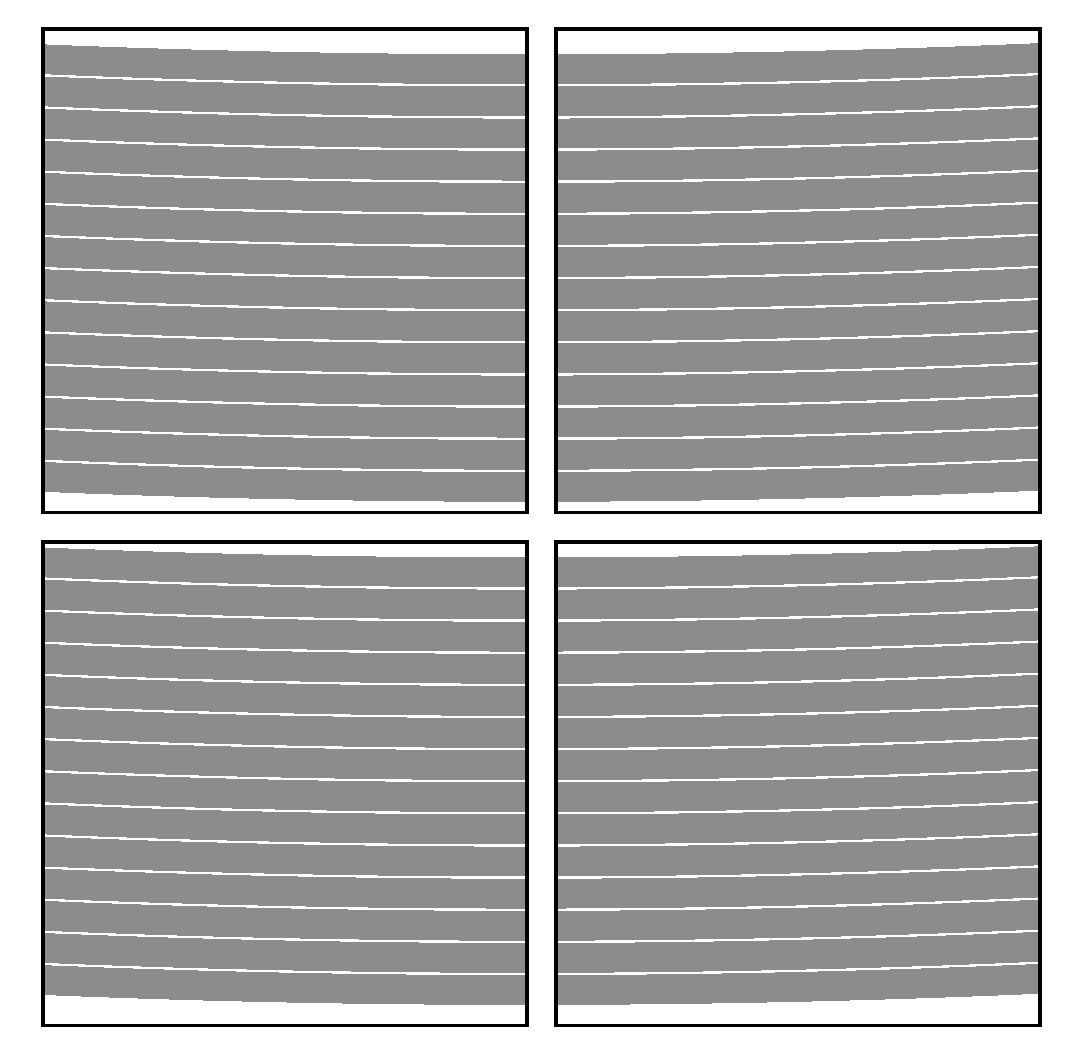
\includegraphics{LMS_detector_layout_normal_tikz}}\hfill
  \resizebox{0.495\textwidth}{!}{%
    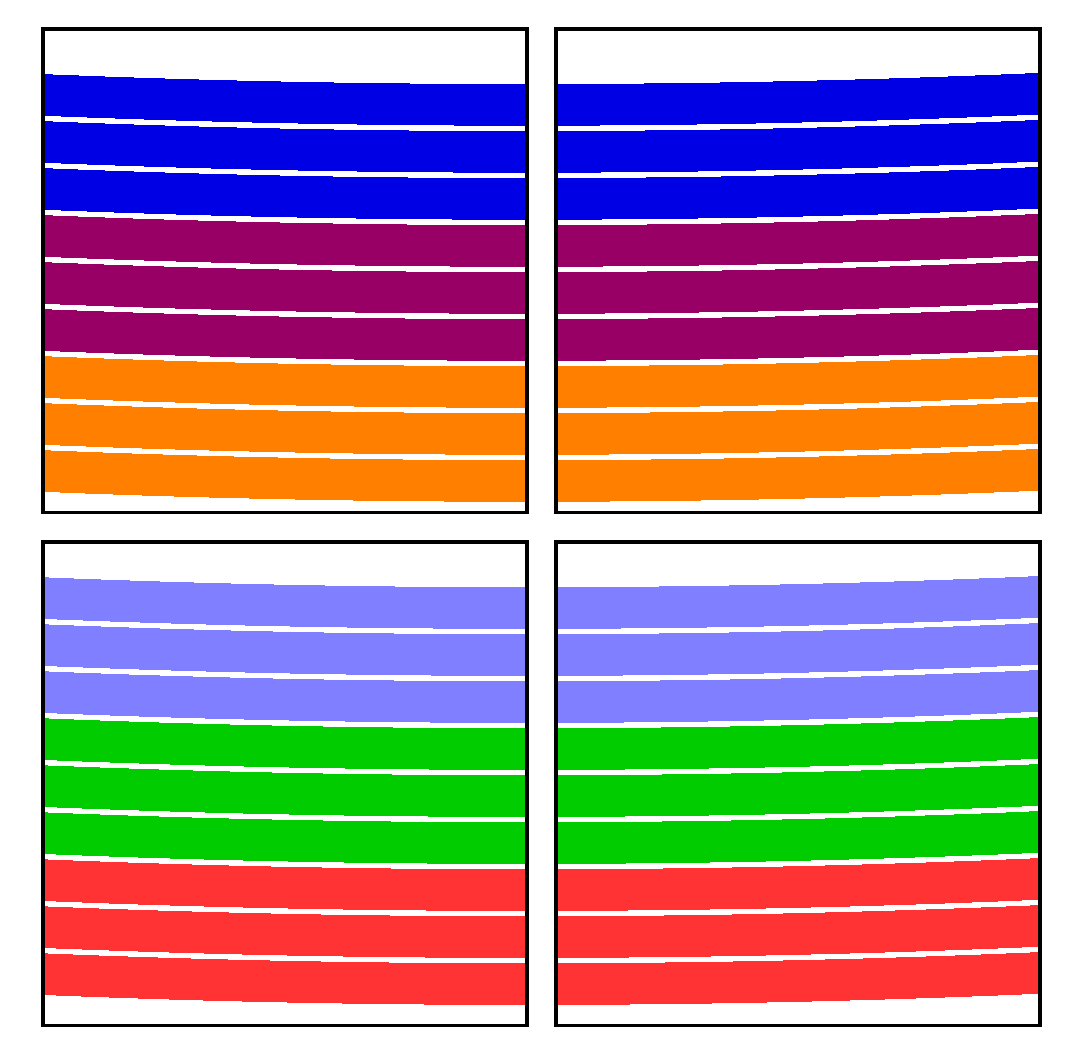
\includegraphics{LMS_detector_layout_extended_tikz}}
  \caption[IFU detector layout]{Layout of the IFU detector mosaic
    in the nominal (left) and extended (right) modes. The dispersion
    direction is horizontal. In the nominal mode, all 28 slices cover
    the same wavelength range. In the extended mode, slices marked by
    the same colour cover the same wavelength ranges, while the
    wavelength ranges of the six groups of slices each are not
    contiguous. The position and curvature of the slices are
    indicative only. }
  \label{fig:IFU_detector_layout}
\end{figure}

The basic templates for LM integral-field spectroscopy are:
\begin{itemize}
\item \lstinline{METIS_ifu_obs_FixedSkyOffset}
\item \lstinline{METIS_ifu_obs_GenericOffset}
\end{itemize}
Both templates move the target position between exposures, using the
internal chopper or the telescope. At a given position a number of
exposures with DIT/NDIT are taken. Depending on the setting of the
template parameter \FITS{DET CUBE MODE} all the DITs may be stored as
layers of a 3D cube (burst mode) or co-added into a 2D image.

As the IFU contains an array of four detectors, there will be four
image or cube extensions in the FITS file for one exposure.

The primary header of the FITS file will contain all information that
pertains to the exposure. This will include information on the
position of the internal chopper, the telescope offsets, and the type
of observation (\FITS{DPR.TYPE=OBJECT} or \FITS{SKY}).

A typical sequence of IFU exposures will go through a series of
dispersion grating settings in order to fill gaps in the instantaneous
wavelength coverage (``spectral dithering''). Finally, the field will be
rotated by 90~degrees and the observing sequence repeated to permit
full image reconstruction
(cf.~Sect.~8.9 of \cite{DRLS}). The FITS header
information will ensure that the position of each exposure within this
complex sequence can be uniquely identified.

%%\begin{center}
%%\begin{table}
%%\caption[IFU data keywords]{Columns foreseen for the IFU FITS files.}
%%\label{tab:lms_colums}
%%\begin{tabular}{|l|l|p{10cm}|}
%%  \hline
%%  \textbf{Column} & \textbf{Format}      & \textbf{Description}                                       \\
%%  \hline
%%  TIME            & long integer         & Time since start of this observation in milliseconds (TBD) \\
%%  \hline
%%  OBSTYPE         & OBJ or SKY           & Exposure on target or on sky?                              \\
%%  \hline
%%  NODDIST         & float (arcsec)       & Nodding distance from reference position                   \\
%%  \hline
%%  CHOPPOS         & $0\dots 360$         & Chopper position angle                                     \\
%%  \hline
%%  CHOPTHROW       & float (mas)          & Chopper distance from reference position                   \\
%%  \hline
%%  CHOPPER         & string               & Flag specifying the position of the internal chopper       \\
%%  \hline
%%  IMAGE1          & 2k$\times$2k integer & raw image from detector 1                                  \\
%%  IMAGE2          & 2k$\times$2k integer & raw image from detector 2                                  \\
%%  IMAGE3          & 2k$\times$2k integer & raw image from detector 3                                  \\
%%  IMAGE4          & 2k$\times$2k integer & raw image from detector 4                                  \\
%%  \hline
%%\end{tabular}
%%\end{table}
%%\end{center}


\subsection{File classification keywords}
\label{ssec:file_classification_keywords}

\TODO{This section will contain the list of files with the values of
  kewords \FITS{DPR.CATG}, \FITS{DPR.TYPE}, \FITS{DPR.TECH}, \FITS{DO
    Category} in accordance with \cite{ESO-DICD}.}

%%%%%%%%%%%%%%%%%%%%%%%%%%%%%%%%%%%%%%%%%%%%%%%%%%%%%%%%%%%%%%%%%%%%%%%%%%%%%%%%
\subsection{Reduced data format}
\label{ssec:reduced_data_format}

All data products, both intermediary and final ones, will be provided in FITS format. Final data products will be saved according to \cite{ESO-products_standard}, fulfilling \REQ{METIS-6061} and \REQ{METIS-6080}.

If there are additional meta-data necessary for archiving, processing, analysis, and distribution, they will be added. \REQ{METIS-6082}.

By default, recipes propagate the FITS headers of the \emph{first raw frame} in
the input \ac{SOF} to the data products. This includes the meteorological,
astronomical and atmospheric site parameters, fulfilling \REQ{METIS-6733}. The same is true for \ac{AO} Telemetry, satisfying \REQ{METIS-9626}.

The saving-functions provided by ESO \ac{CPL}, given the list of input frames, add this list to the headers of data products, thus providing provenance information in compliance with \REQ{METIS-9627}.

The list of individual data products can be found in
Ch.~\ref{sec:drl_data_structures}.

% THE END
%%%%%%%%%%%%%%%%%%%%%%%%%%%%%%%%%%%%%%%%%%%%%%%%%%%%%%%%%%%%%%%%%%%%%%%%%%%%%%%%

%%% Local Variables:
%%% TeX-master: "METIS_DRLD"
%%% End:


% General part on pipeline and DFS
\section{Functional and Workflows Description}
% ESO-037611 expects a section called "Functional and Workflows Description" in the DRLD
% "Data Processing Overview" is the term used for the DRLS.
%\section{Data Processing Overview}
\label{sec:data_processing_overview}

The METIS data reduction system runs in different environments and
serves various purposes.  According to the setting, the following
pipeline levels are distinguished~\cite{1618}:

\begin{description}
\item[Quality Control Level 0 (QC0):] The QC0 pipeline runs
  automatically in real time on a dedicated pipeline workstation in
  the instrument control room at the observatory. Its purpose is to
  analyse every FITS file created by the instrument and produce
  quality control parameters that allow assessment of whether the
  observation and instrument performance were within specifications.
  The appropriate reduction recipe is triggered either when a single
  FITS file is delivered to the workstation or when a template is
  finished. The files are classified based on header keywords, grouped
  and associated to the necessary standard calibration files.

\item[Quality Control Level 1 (QC1):] The goal of the QC1 pipeline is
  to produce certified calibration products from calibration
  observations as well as to produce QC parameters that are used to
  check the quality of observations and to monitor observing
  conditions and instrument health.
  The QC1 pipeline is run automatically by ESO in Garching.
  Calibration products and QC parameters are ingested into the ESO Science Archive.

\item[Quality Control Level 2 (QC2):] The QC2 pipeline produces
  Science Data Products compliant with~\cite{ESO-products_standard} as
  well as QC parameters derived from science exposures. It runs
  offline in an automatic way and uses the best calibration products
  for the night of observation (produced by the QC1 pipeline).
  The QC2 pipeline is run automatically by ESO in Garching.
  Science data products and QC parameters are ingested into the ESO Science Archive.

\item[Science-Grade Desktop Environment:] The pipeline recipes are
  delivered to the astronomical community to enable users to reduce
  data in an optimal and interactive way. Recipes can be run from the
  command line using the \lstinline{esorex} front-end or in the
  context of a \lstinline{Reflex}/\ac{EDPS} workflow. While the desktop recipes
  are identical to those used in the QC2 pipeline, the user can change
  recipe parameters to optimise the reduction. Within the
  \lstinline{Reflex}/\ac{EDPS} environment, interactive tools are provided that
  allow the user to assess the quality of individual reduction steps
  and to repeat them with different parameters. The products of this
  pipeline are compliant with~\cite{ESO-products_standard}.

\end{description}


The rest of this document describes the recipes primarily from the perspective of the desktop pipeline.
The QC0, QC1, QC2 pipelines use the subset of these recipes necessary for the goals described above.
Recipes used in the QC0 environment are written such that they can be run in real time, possibly requiring different defaults for processing parameters.


\subsection{Required calibrations}
\label{ssec:calibrations}

Table~\ref{tab:calibrations_per_mode} (taken from
\cite{METIS-calibration_plan}) lists the main calibration steps that
are required for each instrument mode.

%\TODO{Do we apply NCPA + PSF to HCI data? For ADI a simple recipe is foreseen.} The NCPA estimating algorithms are still under study by the HCI team.
%\begin{landscape}
\begin{table}
  \newcommand{\yes}{\tikz\fill[scale=0.35,color=green!50!black](0,.35) -- (.25,0) -- (0.9,.7) -- (.25,.15) -- cycle;}
  \newcommand{\no}{\textcolor{red!50!black}{---}}
    \caption[Overview of required calibrations per instrument mode]{Overview of required calibrations per instrument mode.
    The IFU modes refer to both the nominal configuration and to the extended wavelength configuration. From~\cite{METIS-calibration_plan}.}
  \label{tab:calibrations_per_mode}
  \centering\scriptsize
  \begin{tabularx}{\textwidth}{lXccXccccc}
    \hline
                           & Dark / Linearity & Flat & Wave & Offset type & Telluric & Flux & Distortion & NCPA + PSF & RSRF \\
    \hline\hline
    \CODE{IMG_LM}          & \yes & \yes & \no  & Dither         & \no      & \yes & \yes       & \no        & \no  \\
    \CODE{IMG_LM_(RA/C)VC} & \yes & \yes & \no  & ADI            & \no      & \yes & \yes       & \yes       & \no  \\
 %   \CODE{IMG_LM_CLC}      & \yes & \yes & \no  & ADI            & \no      & \yes & \yes       & \yes       & \no  \\
    \CODE{IMG_LM_APP}      & \yes & \yes & \no  & Dither + ADI   & \no      & \yes & \yes       & \yes       & \no  \\
    \CODE{SPEC_LM}         & \yes & \no  & \yes & Dither along slit & \yes  & \yes & \yes       & \no        & \yes \\
    \CODE{IFU}             & \yes & \no  & \yes & Dither         & \yes     & \yes & \yes       & \no        & \yes \\
    \CODE{IFU_APP}         & \yes & \no  & \yes & Dither\footnote{Dithering for background subtraction + IFU\_APP will not be practical due to AO halo.}  + ADI  & \yes     & \yes & \yes       & \yes       & \yes \\
    \CODE{IFU_(RA/C)VC}    & \yes  & \no  & \yes & ADI            & \yes     & \yes & \yes       & \yes       & \yes \\
   % \CODE{IFU_CLC}         & \yes & \no  & \yes & Dither + ADI   & \yes     & \yes & \yes       & \yes       & \yes \\
    \hline
    \CODE{IMG_N}           & \yes  & \yes & \no  & chop/nod       & \no      & \yes & \yes       & \no        & \no  \\
    \CODE{IMG_N_CVC}       & \yes  & \yes & \no  & three-point chopping & \no & \yes & \no       & \yes       & \no  \\
 %   \CODE{IMG_N_CLC}       & \no  & \yes & \no  & out-of-field chopping & \no & \yes & \no      & \yes       & \no  \\
    \CODE{SPEC_N_LOW}      & \yes  & \no  & \yes & chop/nod along slit & \yes & \yes & \yes      & \no        & \yes \\
    \hline
  \end{tabularx}
\end{table}
%\end{landscape}
\FloatBarrier

%%%
\subsection{Imaging in LM and N}
\label{ssec:overview_lm_imaging}

% HB 20230731: This note is not really necessary I think.
%\textbf{Note: The pipeline layout has been modified compared to the
%  PDR design in order to achieve better modularity. Basic reduction
%  and background subtraction have been split into two recipes that now
%  are applied to both standard calibration and science data. ADI recipes have been added since PDR however integration of \ac{HCI}
%  into this workflow requires more work: \ac{HCI} images will be treated
%  the same way at least through basic reduction, possibly through
%  background subtraction. \ac{ADI} combination may require a separate
%  recipe, at least for some \ac{HCI} configurations.}

The purpose of the pipeline is to correct or remove contributions from
the instrument, telescope, and atmosphere and produce science-grade
data products.  In the case of the METIS imaging modes the main
contributions to correct or remove are dark current, flatfield, bad
pixels, and, most importantly, thermal background emission from the
sky and the telescope. Further effects include persistence,
cross-talk, geometric distortions, etc. The final product of the
imaging pipeline is one or more image(s) that are flux-calibrated in units of
photons/s/pixel against a standard star.
Several images can be stacked into a single possibly mosaiced image.

Due to the differences in characteristics between the HAWAII2RG
detector used for imaging in the L and M bands and the GeoSnap
detector used for the N band, the operational concept for the two
imager subsystems are quite different. This induces differences in the
way the data have to be reduced.

The GeoSnap detector has more stable gain than AQUARIUS detector,
which was still in the baseline at PDR\@.  Chopping is still necessary, albeit
at a lower frequency of a few Hz, and a chop/nod technique, which meets the
specific ELT requirements (Section~\ref{sssec:nbandsbackgroundsubtracion}),
will be employed  for background subtraction.  As the dark
signal is automatically removed when the exposures from the different
chop and nod positions are combined no master dark is required for the
reduction of science data. The GeoSnap data is also flat fielded.

Observations and reduction of LM band data with the HAWAII2RG detector
can proceed as in the near infrared. After dark subtraction and
flat-fielding, the background is estimated from a series of dithered
science exposures or from exposures on a nearby blank patch of sky.

The association maps for the current designs of the imaging pipelines
in~LM and~N are shown in Figs.~\ref{fig:IMG_LM_Assomap}
and~\ref{fig:IMG_N_Assomap}, respectively.

%\TODO{For \ac{HCI} data, \ac{ADI} may need to be part of reduction recipe if
%  individual background subtracted images are the goal?} We provide ADI recipes since PDR.

\begin{landscape}
  \begin{figure}
    \centering
    \resizebox{\linewidth}{!}{%% IMG_LM_assomap_tikz.tex
%% Created by Oliver Czoske
%%
%% 2019-02-26: Changed to LM only
%% 2019-02-26: Try to align it with the recipe flow
%% 2020-09-07: Pipeline redesign

\sffamily

\input{black_style}
\input{recipe_config}

%%% Picture: flow chart
\begin{tikzpicture}[on grid=false,node distance=0.8cm]

  \matrix (recipes) [column sep=0.1cm, row sep=1cm]{
    % The matrix has colums
    % detlin_*, dark_*, flat_*, std_*, sci1_*, sci2_*, adi
    %
    % The matrix has rows
    % *_raw, *_dark, *_flat, *_std, *_sci1, *_sci2, *_prod

    % Row *_raw
    \node [above] (lin_raw){%
      \recipebox{DETLIN}{det\_lingain}
    };
    &
    \node [above] (pers_raw){%
        \recipebox{PERSISTENCE}{persistence\_map}
    };
    &
    \node [above] (dist_raw){%
      \recipebox{DISTORTION}{lm\_img\_distortion}
    };
    &
    \node[above] (dark_raw) {%
      \recipebox{DARK}{det\_dark}
    };
    &
    \node[above] (flat_raw){%
      \recipebox{FLAT}{lm\_img\_flat}
    };
    &
    \node[above] (all1_raw){%
      \recipebox{SCIENCE, STD}{lm\_img\_basic}
    };
    &
    \node[above] (all2_raw){%
      \recipebox{SCIENCE, STD}{lm\_img\_background}
    };
    &
    \node[above] (std_raw){%
      \recipebox{PHOT STD}{lm\_img\_std\_process}
    };
    &
    \node[above] (sci1_raw){%
      \recipebox{SCIENCE}{lm\_img\_sci\_calibrate}
    };
    &
    \node[above] (sci2_raw){%
      \recipebox{SCIENCE}{lm\_img\_sci\_coadd}
    };

   % \node[above] (sci2_raw){%     % needs width parameter to box
   %  \begin{tcolorbox}[%
   %    width=4.5cm,
   %    colback=recipecolor]
   %    \centering lm\_img\_sci\_postprocess
   %  \end{tcolorbox}};
   %&
   %\node[above] (adi_raw){%
   %  \recipenotitlebox{adi\_postprocess}
   %};
   \\

    %%% Calibration products
    % Row *_lin
    \node (lin_lin) [statcalfile]{\hyperref[dataitem:linearity_2rg]{\STATCALIB{LINEARITY_2RG}}}; &
    \node (pers_lin)[empty]{}; &
    \node (dist_lin)[empty]{}; &
    \node (dark_lin)[empty]{}; &
    \node (flat_lin)[connection]{}; &
    \node (all1_lin)[connection]{}; &
    \node (all2_lin)[empty]{}; &
    \node (std_lin)[empty]{}; &
    \node (sci1_lin)[empty]{}; &
    \node (sci2_lin)[empty]{}; \\

    % Row persistence
    \node (lin_pers)[empty]{}; &
    \node (pers_pers)[extcalfile]{\STATCALIB{PERSISTENCE_MAP}}; &
    \node (dist_pers)[empty]{}; &
    \node (dark_pers)[empty]{}; &
    \node (flat_pers)[connection]{}; &
    \node (all1_pers)[connection]{}; &
    \node (all2_pers)[empty]{}; &
    \node (std_pers)[empty]{}; &
    \node (sci1_pers)[empty]{}; &
    \node (sci2_pers)[empty]{}; \\

    % Row *_dark
    \node (lin_dark) [empty]{}; &
    \node (pers_dark) [empty]{}; &
    \node (dist_dark) [empty]{}; &
    \node (dark_dark) [calibproduct]{\hyperref[dataitem:master_dark_2rg]{\PROD{MASTER_DARK_2RG}}}; &
    \node (flat_dark)[connection]{}; &
    \node (all1_dark)[connection]{}; &
    \node (all2_dark)[empty]{}; &
    \node (std_dark)[empty]{}; &
    \node (sci1_dark)[empty]{}; &
    \node (sci2_dark) [empty]{}; \\

    % Row *_flat
    \node (lin_flat) [empty]{}; &
    \node (pers_flat) [empty]{}; &
    \node (dist_flat)[empty]{}; &
    \node (dark_flat)[empty]{}; &
    \node (flat_flat) [calibproduct]{\hyperref[dataitem:master_flat_2rg]{\PROD{MASTER_FLAT_2RG}}}; &
    \node (all1_flat)[connection]{}; &
    \node (all2_flat)[empty]{}; &
    \node (std_flat)[empty]{}; &
    \node (sci1_flat)[empty]{}; &
    \node (sci2_flat) [empty]{}; \\

    % Row *_all1
    \node (lin_all1)[empty]{}; &
    \node (pers_all1) [empty]{}; &
    \node (dist_all1)[empty]{}; &
    \node (dark_all1)[empty]{}; &
    \node (flat_all1)[empty]{}; &
    \node (all1_all1)[calibproduct]{\hyperref[dataitem:std_reduced]{\PROD{STD_REDUCED}}}; &
    \node (all2_all1)[calibproduct]{\hyperref[dataitem:std_bkg_sub]{\PROD{STD_BKG_SUB}}}; &
    \node (std_all1)[connection]{}; &
    \node (sci1_all1)[empty]{}; &
    \node (sci2_all1) [empty]{}; \\

% Row *_all2
    \node (lin_all2) [empty]{}; &
    \node (pers_all2) [empty]{}; &
    \node (dist_all2)[empty]{}; &
    \node (dark_all2)[empty]{}; &
    \node (flat_all2)[empty]{}; &
    \node (all1_all2)[scienceproduct]{\hyperref[dataitem:sci_reduced]{\PROD{SCI_REDUCED}}}; &
    \node (all2_all2)[scienceproduct]{\hyperref[dataitem:sci_bkg_sub]{\PROD{SCI_BKG_SUB}}}; &
    \node (std_all2)[empty]{}; &
    \node (sci1_all2)[connection]{}; &
    \node (sci2_all2) [empty]{}; \\

    % Row *_dist
    \node (lin_dist) [empty]{}; &
    \node (pers_dist) [empty]{}; &
    \node (dist_dist)[statcalfile]{\hyperref[dataitem:distortion_tab]{\STATCALIB{DISTORTION_TAB}}}; &
    \node (dark_dist)[empty]{}; &
    \node (flat_dist) [empty]{}; &
    \node (all1_dist)[empty]{}; &
    \node (all2_dist)[empty]{}; &
    \node (std_dist)[empty]{}; &
    \node (sci1_dist)[connection]{}; &
    \node (sci2_dist) [empty]{}; \\

    % Row *_std
    \node (lin_std) [empty]{}; &
    \node (pers_std) [empty]{}; &
    \node (dist_std)[empty]{}; &
    \node (dark_std)[extcalfile]{\hyperref[dataitem:fluxstd_catalog]{\EXTCALIB{FLUXSTD_CATALOG}}}; &
    \node (flat_std)[empty]{}; &
    \node (all1_std)[empty]{}; &
    \node (all2_std)[empty]{}; &
    \node (std_std)[connection]{}; &
    \node (sci1_std)[empty]{}; &
    \node (sci2_std) [empty]{}; \\

    % Row *_sci1
    \node (lin_sci1) [empty]{}; &
    \node (pers_sci1) [empty]{}; &
    \node (dist_sci1)[empty]{}; &
    \node (dark_sci1)[empty]{}; &
    \node (flat_sci1)[empty]{}; &
    \node (all1_sci1)[empty]{}; &
    \node (all2_sci1)[empty]{}; &
    \node (std_sci1)[calibproduct]{\hyperref[dataitem:fluxcal_tab]{\PROD{FLUXCAL_TAB}}}; &
    \node (sci1_sci1)[connection]{}; &
    \node (sci2_sci1)[empty]{}; \\

    % Row *_sci2
    \node (lin_sci2) [empty]{}; &
    \node (pers_sci2) [empty]{}; &
    \node (dist_sci2)[empty]{}; &
    \node (dark_sci2)[empty]{}; &
    \node (flat_sci2)[empty]{}; &
    \node (all1_sci2)[empty]{}; &
    \node (all2_sci2)[empty]{}; &
    \node (std_sci2)[empty]{}; &
    \node (sci1_sci2) [scienceproduct]{\hyperref[dataitem:lm_sci_calibrated]{\PROD{LM_SCI_CALIBRATED}}}; &
    \node (sci2_sci2) [connection]{}; \\

    % Row *_prod
    \node(lin_prod) [empty]{}; &
    \node(pers_prod) [empty]{}; &
    \node(dist_prod) [empty]{}; &
    \node(dark_prod) [empty]{}; &
    \node(flat_prod) [empty]{}; &
    \node(all1_prod) [empty]{}; &
    \node(all2_prod) [empty]{}; &
    \node(std_prod) [empty]{}; &
    \node(sci1_prod) [empty]{}; &
    \node (sci2_prod)[scienceproduct]{\hyperref[dataitem:lm_sci_coadd]{\PROD{LM_SCI_COADD}}}; \\
  };    % end matrix

  \node (t1) at ($(dist_raw)!0.5!(dark_raw)$){};
  \node (t2) at ($(dist_prod)!0.5!(dark_prod)$){} ;
  \draw [thick,dashed] ([yshift=8mm]t1.north) -- ([yshift=-8mm]t2.south);



  %% Vertical connections
  \draw [arrow] (lin_raw)  -- (lin_lin);
  \draw [arrow] (pers_raw) -- (pers_pers);
  \draw [arrow] (dist_raw) -- (dist_dist);
  \draw [arrow] (dark_raw) -- (dark_dark);
  \draw [arrow] (flat_raw) -- (flat_flat);
  \draw [arrow] (all1_raw) -- (all1_all1);
  \draw [arrow] (all1_all1) -- (all1_all2);
  \draw [arrow] (std_all1) -- (std_sci1);
  \draw [arrow] (sci1_all2) -- (sci1_sci2);
  \draw [arrow] (sci2_sci2) -- (sci2_prod);
%  \draw [arrow] (adi_sci2) -- (adi_prod);

  %% Horizontal connections
  \draw [match] (lin_lin)   -- (all1_lin);
  \draw [match] (pers_pers) -- (all1_pers);
  \draw [match] (dark_dark) -- (all1_dark);
  \draw [match] (flat_flat) -- (all1_flat);
  \draw [match] (all1_all1) -- (all2_all1);
  \draw [match] (all2_all1) -- (std_all1);
  \draw [match] (all1_all2) -- (all2_all2);
  \draw [match] (all2_all2) -- (sci1_all2);
  \draw [match] (sci1_std) -- (sci1_sci1);
  \draw [match] (dist_dist) -- (sci1_dist);
  \draw [match] (dark_std) -- (std_std);
  \draw [match] (std_sci1) -- (sci1_sci1);
  \draw [match] (sci1_sci2) -- (sci2_sci2);

  %% Legend
  \matrix (legend) [draw, fill=gray!15, above right, row sep=0.3cm,
    column 1/.style={anchor=base},
    column 2/.style={anchor=base west}]
    at ([yshift=0ex]current bounding box.south west){%
      \node (leg_recipe) [recipe] {lm\_img\_flat};
      & \node {recipe}; \\
      \node (leg_calproduct) [calibproduct] {MASTER\_DARK\_2RG};
      & \node {calib.\ product}; \\
      \node (leg_sciproduct)[scienceproduct] {LM\_SCI\_REDUCED};
      & \node {science product}; \\
      \node (leg_statcalfile)[statcalfile] {MASTER\_RSRF};
      & \node {static calib.\ file};\\
      \node (leg_calfile)[extcalfile]{FLUXSTD\_CATALOG};
      & \node {external calib.\ file}; \\

    \draw [arrow,fill=black] (0,0.4) -- (0,-0.3);  %% should be centred relative to column
    & \node {processing step}; \\

    \draw (-1, 0.5ex) -- (1,0.5ex) node [connection,yshift=0cm]{};
    & \node {product match}; \\
  };    %% end matrix (legend)

\end{tikzpicture}
}
    \caption[Reduction cascade and association map for imaging in L and
      M]{Association map for imaging in the LM band. The figure shows only
      the primary product created from each recipe; for a full list of
      products refer to the recipe descriptions in
      Sect.~\ref{ssec:recipes_img_lm}. The dashed line separates
      calibration tasks that are done at AIT or infrequently during
      operations (left) from daily tasks (right). The prefix ``\texttt{metis\_}'' has been
      omitted from the recipe names to improve clarity.}
    \label{fig:IMG_LM_Assomap}
  \end{figure}
\end{landscape}

\begin{landscape}
\begin{figure}
  \centering
    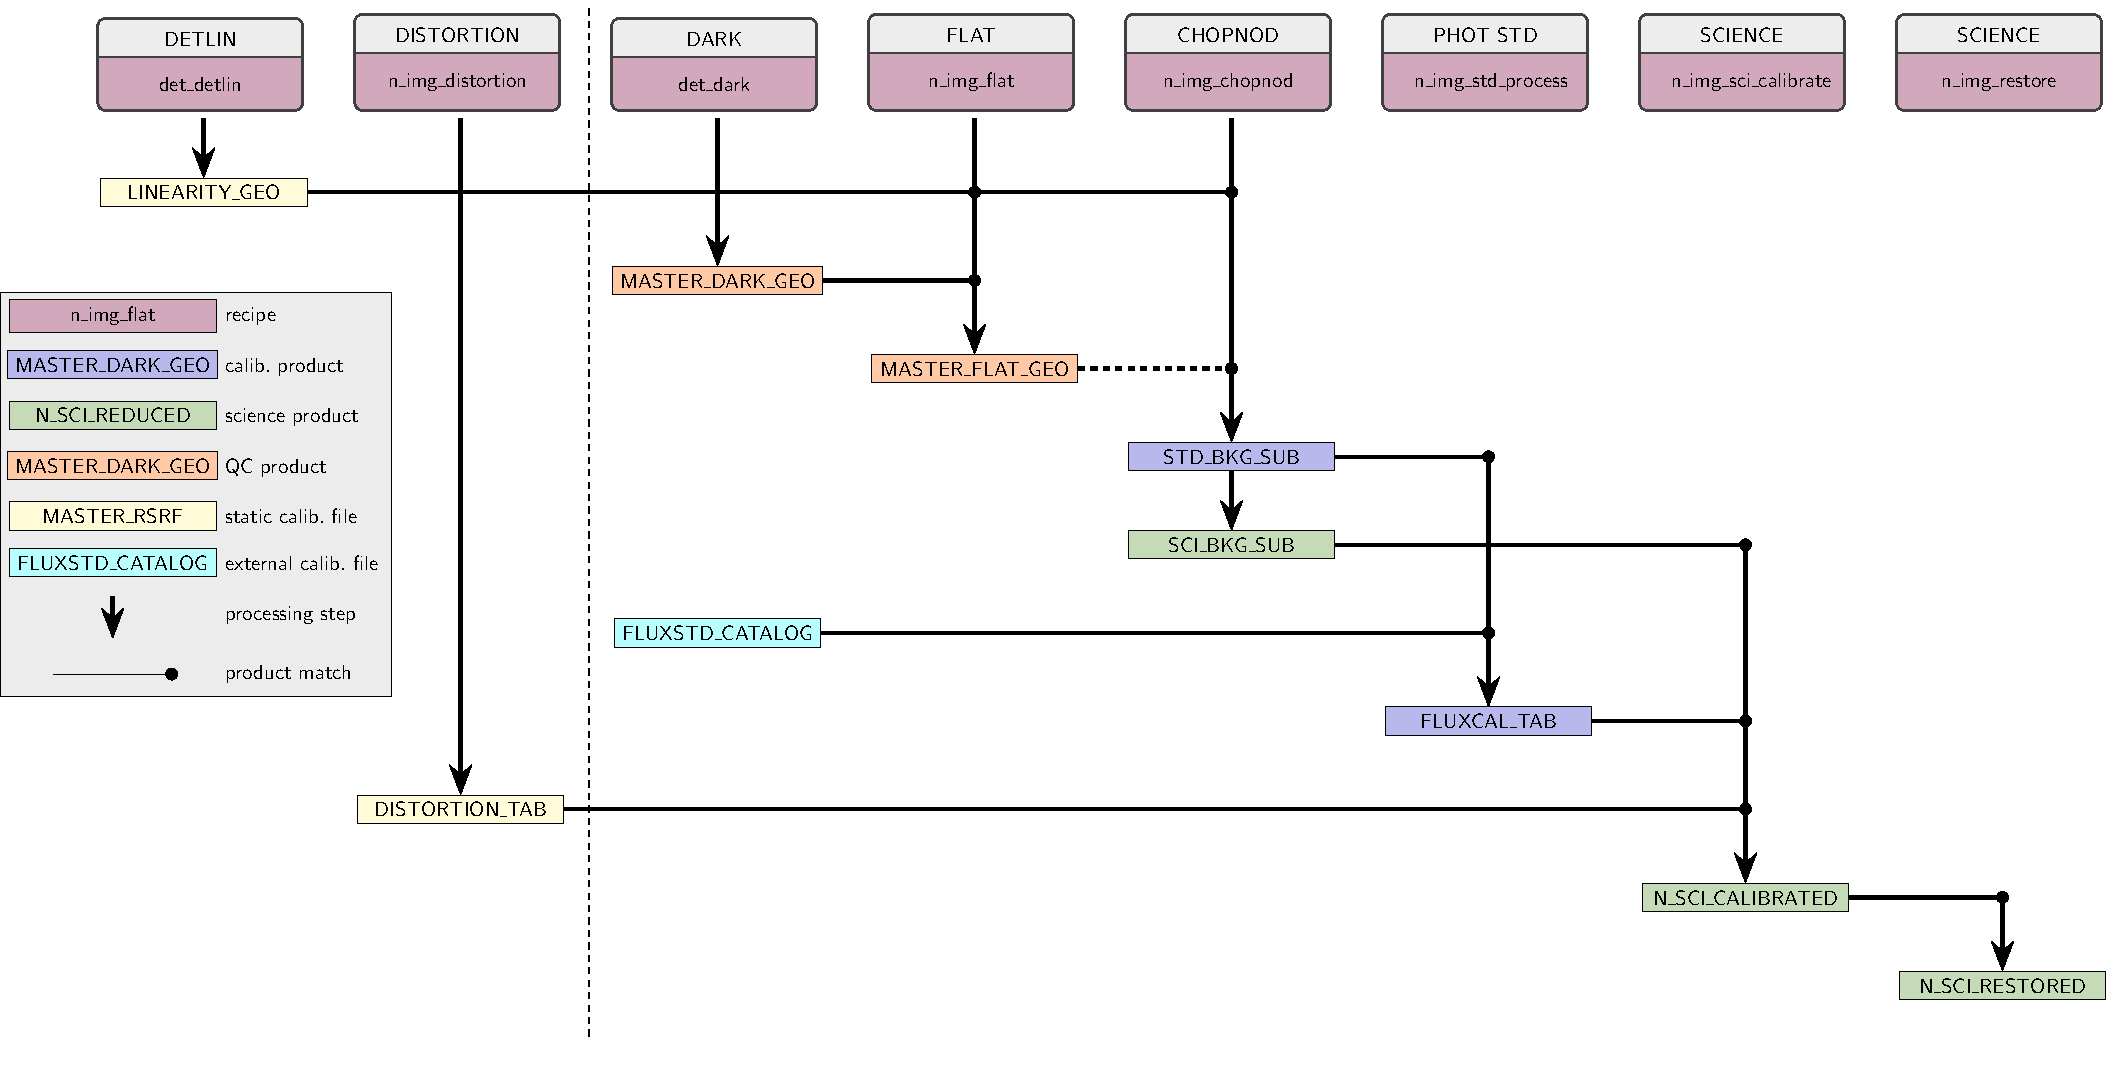
\includegraphics{IMG_N_assomap_tikz}
    \caption[Reduction cascade and association map for imaging in N]{%
      Association map for imaging in the N band. The figure shows
      only the primary product created from each recipe; for a full
      list of products refer to the recipe descriptions in
      Sect.~\ref{ssec:recipes_img_n}. The dashed line separates
      calibration tasks that are done at AIT or infrequently during
      operations (left) from daily tasks (right). The prefix ``\texttt{metis\_}'' has
      been omitted from the recipe names to improve clarity.}
    \label{fig:IMG_N_Assomap}
  \end{figure}
\end{landscape}

%%%%%%%%%%%%%%%%%%%%%%%%%%%%%%%%%%%%%%%%%%%%%%%%%%%%%%
%%% Local Variables:
%%% TeX-master: "METIS_DRLD"
%%% End:


%%%
\subsection{Long-Slit Spectroscopy in L/M- and N-bands}\label{lss:overview}
\subsubsection{The workflow cascades}\label{lss:cascade_overview}
The purpose of the pipeline is to correct or remove contributions from
the instrument, telescope, and atmosphere and generate science-grade
data products for the L/M- and N-band \ac{LSS}
mode. Since the detector properties are not fully specified, especially of the new Geosnap, we currently assume
basically the same reduction cascade for both spectral ranges LM and
N, respectively. The only major difference at the time being is the absence of \ac{WCU} laser sources in the N-band, which are only available during \ac{AIT} phase to generate a first guess of the pixel-to-wavelength relation. Therefore the first guess wavelength solution in the N-band will be based on that \ac{AIT} data. As we assume the instrument to be very stable, that approach should be sufficient for the low-resolution N-band spectroscopy. In the LM range, two fix-frequency lasers ($@3.39$µm and $@5.26$µm) and one tuneable ($4.68....4.78$µm) is foreseen in the \ac{WCU} to be taken on daily basis (cf. \cite{METIS-calibration_plan}). Although mainly foreseen to be used for the high-resolution spectroscopy \ac{LMS} mode, we can use these laser sources for the LM-band \ac{LSS} as well.

Special emphasis has to be drawn to the effects of the Earth's
atmosphere in several respects:
\begin{itemize}
\item Wavelength calibration: Absorption/emission features are intended to be
  used for the wavelength calibration. Thus, a good knowledge on /
  identification of these features is crucial for the accuracy of the
  wavelength calibration.
\item Telluric correction: In the MIR regime telluric absorption is
  one of the most dominant effects visible in spectra. Modelling
  approaches like \texttt{molecfit} heavily rely on accurate
  atmospheric input profiles, which represent the actual state and
  composition of the Earth's atmosphere. This especially applies to
  the \ac{PWV} content since this is the most
  dominant and most variable species.
\item Atmospheric dispersion: \ac{METIS} will have \ac{ADC}s compensating the
  effect of atmospheric dispersion. However, for technical reasons
  these ADCs are fixed at several positions. This means that the
  compensation is only partially. This leads to two practical effects:
  (a) wavelength-dependent slit losses, and (b) distortions in both,
  the spatial and the spectral direction (see \cite{METIS-ADC_study}
  for more details). For both, the pipeline needs to correct
  for. It is foreseen to determine these slitlosses on yearly basis with a separate calibration task (cf. \cite{METIS-calibration_plan}) and create a slit-loss table to be included in the static calibration database.
\end{itemize}

%However, to keep flexibility and independence of both branches, we
%define different recipes for the time being, although they will be
%mostly based on the same algorithms. We therefore focus here on the LM-band only.

Figures~\ref{Fig:LMLssAssomap1} and \ref{Fig:LMLssAssomap2} show the reduction cascade and the association map for the recipes handling L/M-long-slit
spectroscopy data.  Table~\ref{Tab:LMLssDatProc} contains the data processing table for this mode. For the N-band \ac{LSS} mode the cascade and the data processing table is given in Fig.\ref{Fig:NLssAssomap} and Table~\ref{Tab:NLssDatProc}, respectively (cf. also Fig.~\ref{Fig:LSScascadelegend}).

In general, there are four major steps in each of the two cascades:
\begin{itemize}
    \item \textbf{Preparation step:} This contains the recipes, which are invoked only rarely, e.g. after major instrument interventions, or on monthly/yearly basis to update the static calibration database. These recipes are therefore not shown in the cascade in Figs.~\ref{Fig:LMLssAssomap1}/\ref{Fig:LMLssAssomap2} and \ref{Fig:NLssAssomap} and the corresponding data processing tables. In case of the \ac{LSS} pipeline this concerns the creation of the gain maps/linearity checks (see Section~\ref{sssec:metis_det_lingain}), the determination of the slit losses induced by the fixed positions of the ADCs (cf. Section~\ref{sssec:adc_slitlosses} and Section "Calibration of slit losses" in Calibration plan \cite{METIS-calibration_plan}) and the zero position of the chopping mirror (see Section~\ref{ssec:metisimgchophome} and Section "Chopper Home Position" in \cite{METIS-calibration_plan} for more details). T
    \item \textbf{Basic steps}: The basic steps aim for correcting the detector influence, in particular the dark correction and the determination of the master \ac{RSRF}.
    \item \textbf{Calibration/correction steps}: This is the main part which incorporates the order trace detection, distortion, wavelength and flux correction.
    \item \textbf{Post-calibration steps}: After havig calibrated spectra at hand, the last step is the telluric absorption correction.
\end{itemize}

\begin{figure}[ht]
  \centering
  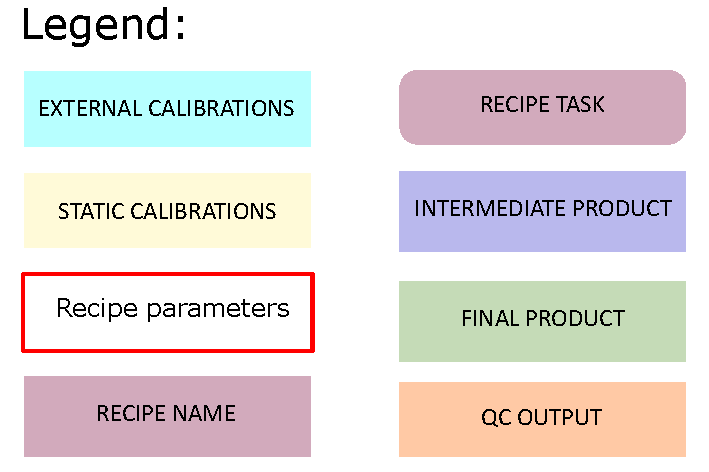
\includegraphics[width=0.4\textheight]{figures/legend.pdf}
  \caption[Legend]{Legend of the coloured boxes in the \ac{LSS} cascades.}
  \label{Fig:LSScascadelegend}
\end{figure}
\clearpage

\begin{sidewaysfigure}[ht]
  \centering
  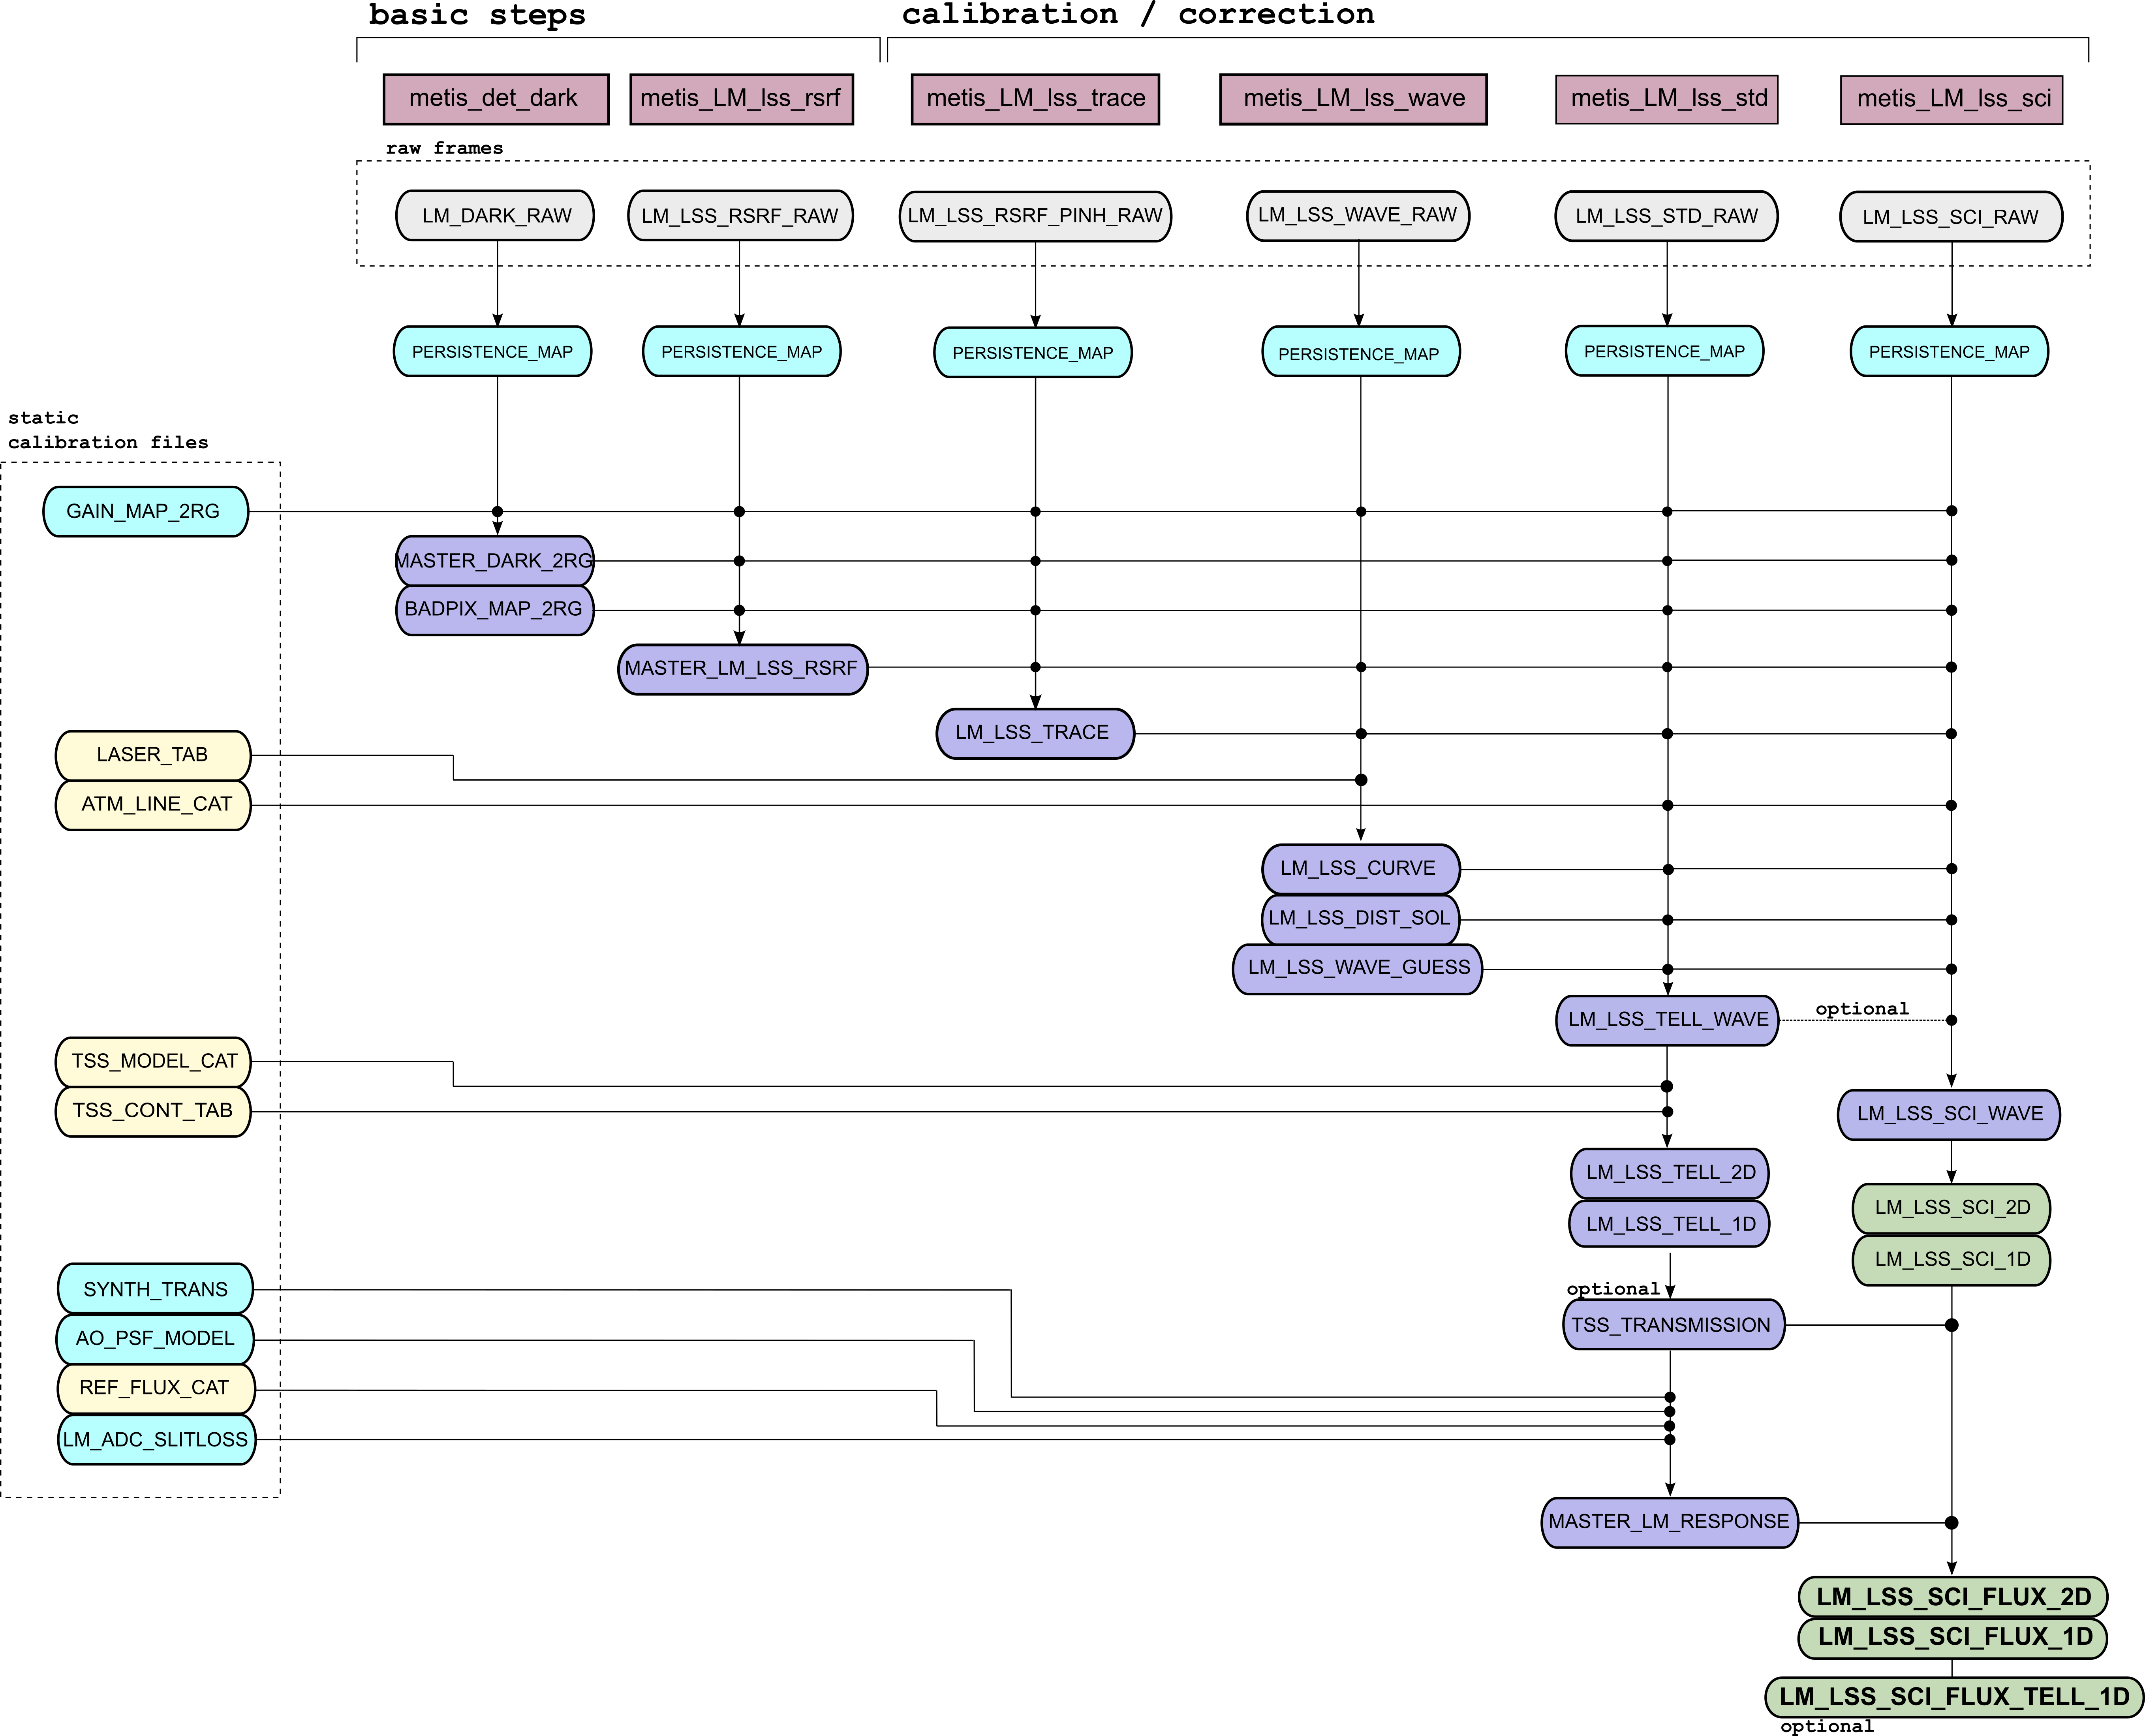
\includegraphics[width=0.9\textheight]{figures/LM_LSS_pipeline_wf_draft_latest_part_1_v0.80.png}
  \caption[Reduction cascade and association map for LM long-slit
  spectroscopy]{Part 1 of the reduction cascade and association map for long-slit
    spectroscopy in the LM bands.  }
  \label{Fig:LMLssAssomap1}
\end{sidewaysfigure}

\begin{sidewaysfigure}[ht]
  \centering
  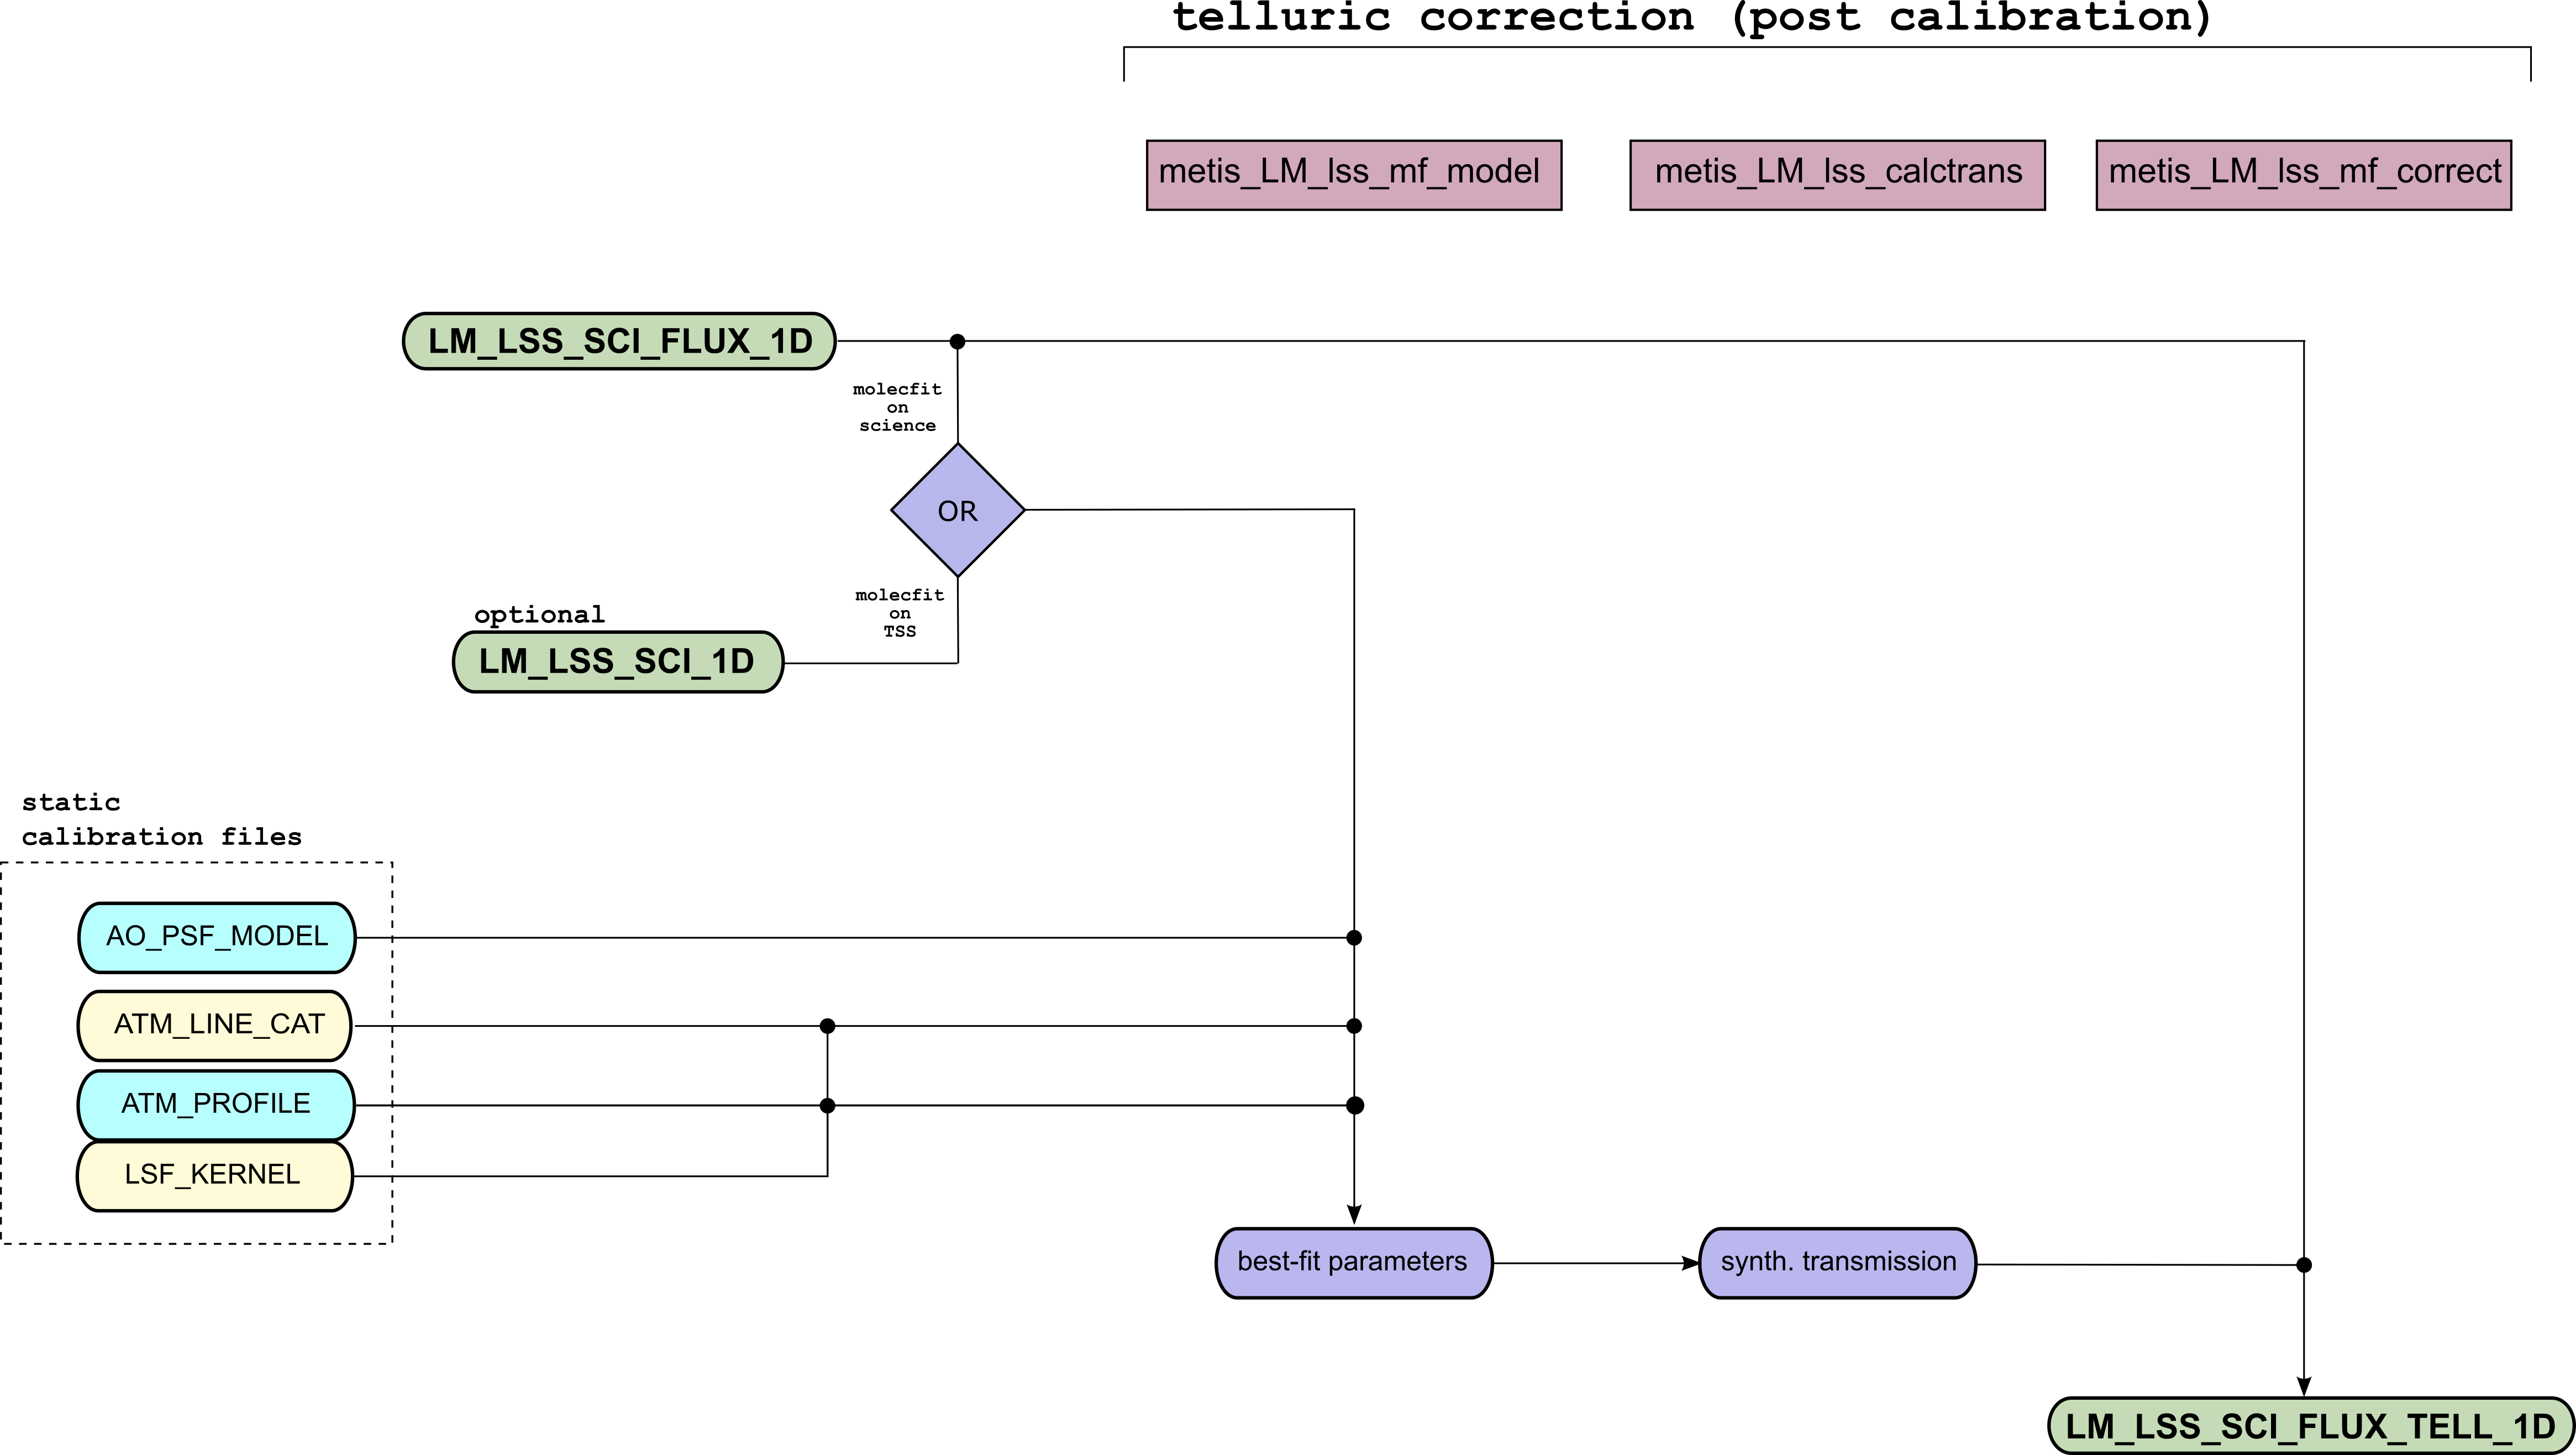
\includegraphics[width=0.8\textheight]{figures/LM_LSS_pipeline_wf_draft_latest_part_2_v0.80.png}
  \caption[Reduction cascade and association map for LM long-slit
  spectroscopy]{Part 2 of the reduction cascade and association map for long-slit
    spectroscopy in the LM bands.  }
  \label{Fig:LMLssAssomap2}
\end{sidewaysfigure}


% \begin{sidewaysfigure}[ht]
%   \centering
%   \includegraphics[width=0.9\textheight]{figures/NQ_LSS_pipeline_wf_draft_latest.png}
%   \caption[Reduction cascade and association map for N long-slit
%   spectroscopy]{Reduction cascade and association map for long-slit
%     spectroscopy in the N band.  }
%   \label{Fig:NQLssAssomap}
% \end{sidewaysfigure}


%% ---- Table: LM long-slit spectroscopy
\begin{sidewaystable}
  \footnotesize
  \begin{center}
    \caption[Data Processing table for LM long-slit spectroscopy]{%
      Data Processing table for LM long-slit spectroscopy
      calibration mode; }\bigskip
    \label{Tab:LMLssDatProc}
    \begin{tabular}{|l|l|l|l|l|l|}
      \hline
      Data Type   & Classification & Recipe (Level)	& FITS Keywords & static CalibDB & Products\\
    (Templates) & Keywords	 & Processing steps	&		&	  &	\\
    \hline
    \TPL{DARK}	& \CODE{DPR.CATG==CALIB} & \hyperref[sssec:metis_det_dark]{\REC{metis_det_dark}} & Exposure time	&	\hyperref[dataitem:gainmap2rg]{\PROD{GAIN_MAP_2RG}}& Averaged dark frame\\
    		& \CODE{DPR.TYPE==DARK}  &			&		&	& Bad pixel map\\
    		& \CODE{DPR.TECH==IMAGE}  &			&		&	& \\
    \hline
    \TPL{FLAT}	& \CODE{DPR.CATG==CALIB} & \hyperref[rec:lsslmrsrf]{\REC{metis_LM_lss_rsrf}} & Exposure time	& \hyperref[dataitem:gainmap2rg]{\PROD{GAIN_MAP_2RG}}	& Averaged, normalized flatfield\\
    		& \CODE{DPR.TYPE==FLAT}  &			&	Grism	& 	& \\
    		& \CODE{DPR.TECH==SPECTRUM}  &			&	Slit	&	& \\
    \hline
         	& \CODE{DPR.CATG==CALIB} &\hyperref[rec:lsslmtrace]{\REC{metis_LM_lss_trace}} & Exposure time	& \hyperref[dataitem:gainmap2rg]{\PROD{GAIN_MAP_2RG}}	& Order location\\
    		& \CODE{DPR.TYPE==FLAT}  &			&		&	& (polynomial fit)\\
    		& \CODE{DPR.TECH==SPECTRUM}  &			&		&	& \\
    \hline
    \TPL{WAVE,LASER} & \CODE{DPR.CATG==CATG} &\hyperref[rec:lsslmwave]{\REC{metis_LM_lss_wave}} & Exposure time &  \hyperref[dataitem:gainmap2rg]{\PROD{GAIN_MAP_2RG}} & wavelength solution\\
    		& \CODE{DPR.TYPE==WAVE,LASER}   &			   & Grism & \hyperref[dataitem:lasertab]{\STATCALIB{LASER_TAB}} &\\
    		& \CODE{DPR.TECH==SPECTRUM}  &			& Slit		&	& \\
    		& \CODE{PRO.CATG==SPECTRUM}   &  &  & & \\
    \hline
    \TPL{FLUX,STD} & \CODE{DPR.CATG==CALIB} & \hyperref[rec:lsslmstd]{\REC{metis_LM_lss_flux}}& Object name (Flux STD) & \hyperref[dataitem:gainmap2rg]{\PROD{GAIN_MAP_2RG}} & Instrumental\\
    		& \CODE{DPR.TYPE==FLUX,STD}   &			   & Exposure time & \hyperref[dataitem:atmlinecat]{\EXTCALIB{ATM_LINE_CAT}} & response function\\
    		& \CODE{DPR.TECH==SPECTRUM}  &			&	Grism	&	\hyperref[dataitem:lmsynthtrans]{\STATCALIB{LM_SYNTH_TRANS}}& \\
    		& \CODE{PRO.CATG==SPECTRUM}   &  & Slit & \hyperref[dataitem:lmadcslitloss]{\STATCALIB{LM_ADC_SLITLOSS}} & \\
    		& & & & \hyperref[dataitem:aopsfmodel]{\EXTCALIB{AO_PSF_MODEL}} &\\    
    		& & & & \hyperref[dataitem:reffluxcat]{\STATCALIB{REF_FLUX_CAT}} &\\    \hline
    \TPL{SCIENCE} & \CODE{DPR.CATG==SCIENCE} & \hyperref[rec:lsslmsci]{\REC{metis_LM_lss_sci}} & Object name &  \hyperref[dataitem:gainmap2rg]{\PROD{GAIN_MAP_2RG}} & Science grade spectrum\\
    		& \CODE{DPR.TYPE==OBJECT}   &			   & Exposure time & \hyperref[dataitem:lmadcslitloss]{\STATCALIB{LM_ADC_SLITLOSS}} &\\
    		& \CODE{DPR.TECH==SPECTRUM}  &			&	Grism	& \hyperref[dataitem:atmlinecat]{\EXTCALIB{ATM_LINE_CAT}}	& \\
    		& \CODE{PRO.CATG==SPECTRUM}   &  & Slit  &  & \\
    \hline
            & \CODE{DPR.CATG==SCIENCE} & \hyperref[rec:LMLSSmfmodel]{\REC{metis_LM_lss_mf_model}} & Object name & \hyperref[dataitem:lsfkernel]{\STATCALIB{LSF_KERNEL}}	 & Best-fit \\
    		& \CODE{DPR.TYPE==OBJECT}   &			  & & \hyperref[dataitem:atmprofile]{\EXTCALIB{ATM_PROFILE}}  & \texttt{molecfit} parameters\\
    		& \CODE{DPR.TECH==TBD}  &			&		& \hyperref[dataitem:atmlinecat]{\EXTCALIB{ATM_LINE_CAT}}	& \\
    		& \CODE{PRO.CATG==TBD}   &  &  & start parameter set & \\
    \hline
            & \CODE{DPR.CATG==SCIENCE} &  \hyperref[rec:LMLSSmfcalctrans]{\REC{metis_LM_lss_mf_calctrans}} & Object name & \hyperref[dataitem:atmlinecat]{\EXTCALIB{ATM_LINE_CAT}}	 & synthetic \\
    		& \CODE{DPR.TYPE==LSS}   &		&	   &   & Transmission curve\\
    		& \CODE{DPR.TECH==TBD}  &			&		& 	& \\
    		& \CODE{PRO.CATG==TBD}   &  &  & & \\
    \hline
            & \CODE{DPR.CATG==SCIENCE} &  \hyperref[rec:LMLSSmfcorrect]{\REC{metis_LM_lss_mf_correct}} & Object name & 	 & Absorption corrected\\
    		& \CODE{DPR.TYPE==LSS}   &			   & & synthetic Transmission curve  & science spectrum\\
    		& \CODE{DPR.TECH==TBD}  &			&		&	& \\
    		& \CODE{PRO.CATG==TBD}   &  &  & & \\
    \hline
    \end{tabular}
  \end{center}
\end{sidewaystable}

\begin{sidewaysfigure}[ht]
  \centering
  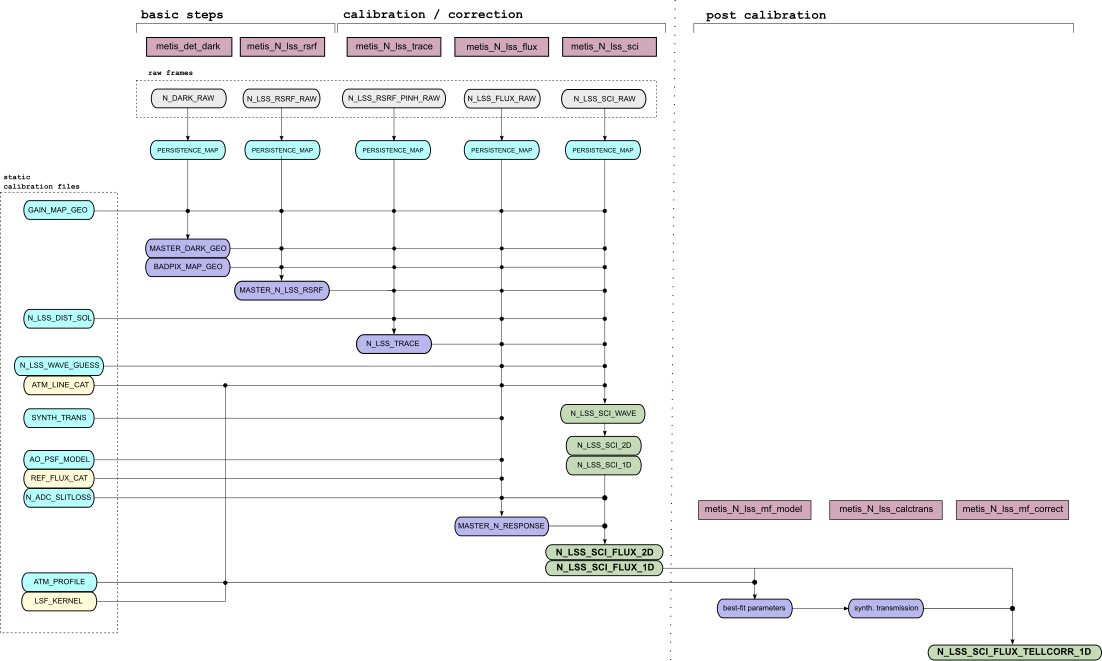
\includegraphics[width=0.9\textheight]{figures/N_LSS_pipeline_wf_draft_latest_v0.74.png}
  \caption[Reduction cascade and association map for N long-slit
  spectroscopy]{Reduction cascade and association map for long-slit
    spectroscopy in the N bands. }
  \label{Fig:NLssAssomap}
\end{sidewaysfigure}

%% ---- Table: N long-slit spectroscopy
\begin{sidewaystable}
  \footnotesize
  \begin{center}
    \caption[Data Processing table for N-band long-slit spectroscopy]{%
      Data Processing table for N long-slit spectroscopy
      calibration mode}\bigskip
    \label{Tab:NLssDatProc}
    \begin{tabular}{|l|l|l|l|l|l|}
      \hline
      Data Type   & Classification & Recipe (Level)	& FITS Keywords & static CalibDB & Products\\
    (Templates) & Keywords	 & Processing steps	&		&	  &	\\
    \hline
    \TPL{DARK}	& \CODE{DPR.CATG==CALIB} & \hyperref[sssec:metis_det_dark]{\REC{metis_det_dark}} & Exposure time	& \hyperref[dataitem:gainmap2rg]{\PROD{GAIN_MAP_GEO}}	& Averaged dark frame\\
    		& \CODE{DPR.TYPE==DARK}  &			&		&	& Bad pixel map\\
    		& \CODE{DPR.TECH==IMAGE}  &			&		&	& \\
    \hline
    \TPL{FLAT}	& \CODE{DPR.CATG==CALIB} & \hyperref[rec:lssnrsrf]{\REC{metis_N_lss_rsrf}} & Exposure time	& \hyperref[dataitem:gainmap2rg]{\PROD{GAIN_MAP_GEO}}	& Averaged, normalized flatfield (\ac{RSRF}\\
    		& \CODE{DPR.TYPE==FLAT}  &			&	Grism	&	& Bad pixel map\\
    		& \CODE{DPR.TECH==SPECTRUM}  &			& Slit		&	& \\
    \hline
         	& \CODE{DPR.CATG==CALIB} & \hyperref[rec:lssntrace]{\REC{metis_N_lss_trace} }& Exposure time	& \hyperref[dataitem:gainmap2rg]{\PROD{GAIN_MAP_GEO}}	& Order location\\
    		& \CODE{DPR.TYPE==FLAT}  &			&	Grism	&	& (polynomial fit)\\
    		& \CODE{DPR.TECH==SPECTRUM}  &			&	Slit	&	& \\
    \hline
    \TPL{FLUX,STD} & \CODE{DPR.CATG==CALIB} & \hyperref[rec:lssnflux]{\REC{metis_N_lss_flux}} & Object name (Flux STD) & \hyperref[dataitem:gainmap2rg]{\PROD{GAIN_MAP_GEO}} & Instrumental\\
    		& \CODE{DPR.TYPE==FLUX,STD}   &			   & Exposure time & \hyperref[dataitem:nlsswaveguess]{\STATCALIB{N_LSS_WAVE_GUESS}} & response function\\
    		& \CODE{DPR.TECH==SPECTRUM}   &			   & Grism		& \hyperref[dataitem:atmlinecat]{\EXTCALIB{ATM_LINE_CAT}}	& \\
    		& \CODE{PRO.CATG==SPECTRUM}   &  &  Slit & \hyperref[dataitem:nsynthtrans]{\STATCALIB{N_SYNTH_TRANS}} & \\
    		& & & & \hyperref[dataitem:nadcslitloss]{\STATCALIB{N_ADC_SLITLOSS}} &\\
    		& & & &  \hyperref[dataitem:reffluxcat]{\STATCALIB{REF_FLUX_CAT}} &\\
    		& & & & \hyperref[dataitem:aopsfmodel]{\EXTCALIB{AO_PSF_MODEL}} &\\
    		& & & & \hyperref[dataitem:nlssdistsol]{\STATCALIB{N_LSS_DIST_SOL}} &\\
    		& & & & \hyperref[dataitem:reffluxcat]{\STATCALIB{REF_FLUX_CAT}} &\\
    \hline
    \TPL{SCIENCE} & \CODE{DPR.CATG==SCIENCE} & \hyperref[rec:lssnsci]{\REC{metis_N_lss_sci}} & Object name & \hyperref[dataitem:gainmap2rg]{\PROD{GAIN_MAP_GEO}}  & Science grade spectrum\\
    		& \CODE{DPR.TYPE==OBJECT}   &			   & Exposure time &  \hyperref[dataitem:atmlinecat]{\EXTCALIB{ATM_LINE_CAT}} &\\
    		& \CODE{DPR.TECH==SPECTRUM}  &			&	Grism	&\hyperref[dataitem:nadcslitloss]{\STATCALIB{N_ADC_SLITLOSS}}	& \\
    		& \CODE{PRO.CATG==SPECTRUM}   &  & Slit & \hyperref[dataitem:nlsswaveguess]{\STATCALIB{N_LSS_WAVE_GUESS}} & \\
    		& & & & \hyperref[dataitem:nlssdistsol]{\STATCALIB{N_LSS_DIST_SOL}} &\\
    \hline
            & \CODE{DPR.CATG==SCIENCE} & \hyperref[rec:NLSSmfmodel]{\REC{metis_N_lss_mf_model}} & Object name & \hyperref[dataitem:lsfkernel]{\STATCALIB{LSF_KERNEL}}	 & Best-fit \\
    		& \CODE{DPR.TYPE==OBJECT}   &			  & & \hyperref[dataitem:atmprofile]{\EXTCALIB{ATM_PROFILE}}  & \texttt{molecfit} parameters\\
    		& \CODE{DPR.TECH==TBD}  &			&		& \hyperref[dataitem:atmlinecat]{\EXTCALIB{ATM_LINE_CAT}}	& \\
    		& \CODE{PRO.CATG==TBD}   &  &  & start parameter set & \\
    \hline
            & \CODE{DPR.CATG==SCIENCE} & \hyperref[rec:NLSSmfcalctrans]{\REC{metis_N_lss_mf_calctrans}} & Object name & \hyperref[dataitem:atmlinecat]{\EXTCALIB{ATM_LINE_CAT}}	 & synthetic \\
    		& \CODE{DPR.TYPE==LSS}   &		&	   &  & Transmission curve\\
    		& \CODE{DPR.TECH==TBD}  &			&		&  	& \\
    		& \CODE{PRO.CATG==TBD}   &  &  & & \\
    \hline
            & \CODE{DPR.CATG==SCIENCE} & \hyperref[rec:NLSSmfcorrect]{\REC{metis_N_lss_mf_correct}} & Object name & 	 & Absorption corrected\\
    		& \CODE{DPR.TYPE==LSS}   &			   &  & synthetic Transmission curve & science spectrum\\
    		& \CODE{DPR.TECH==TBD}  &			&		&	& \\
    		& \CODE{PRO.CATG==TBD}   &  &  & & \\
    \hline
    \end{tabular}
  \end{center}
\end{sidewaystable}

\subsubsection{Static calibration database}\label{lss:static_calib}
The static calibration database comprises several data sets, some are updated from time to time:
\begin{itemize}
    \item \hyperref[dataitem:gainmap2rg]{\hyperref[dataitem:gainmap2rg]{\PROD{GAIN_MAP_2RG}}} and \hyperref[dataitem:gainmapgeo]{\hyperref[dataitem:gainmap2rg]{\PROD{GAIN_MAP_GEO}}}: These are the detector gain maps of the detectors (2RG=Hawaii2RG, LM-band; GEO=Geosnap, N-band), which are created by the recipe \hyperref[sssec:metis_det_lingain]{\REC{metis_det_lingain}} (see Section~\ref{sssec:metis_det_lingain}). This recipe also checks the linearity of the pixels and is carried out every once in a while (yearly, TBD, see \cite{METIS-calibration_plan}) as we assume the detectors to be fairly stable.
    \item \hyperref[dataitem:lasertab]{\STATCALIB{LASER_TAB}}: The \ac{WCU} provides laser sources for the first guess of the wavelength solution. The main laser frequencies are fixed (\cite{METIS-calibration_plan}) and given in a static table.
    \item \hyperref[dataitem:atmlinecat]{\EXTCALIB{ATM_LINE_CAT}}: The main wavelength calibration will be done by means of atmospheric lines, most probably based on the \ac{HITRAN}\footnote{\url{https://hitran.org/}}. They are given in a static catalogue. This database is also required by the telluric correction package \texttt{molecfit}.
    \item \hyperref[dataitem:lmsynthtrans]{\STATCALIB{LM_SYNTH_TRANS}}/\hyperref[dataitem:nsynthtrans]{\STATCALIB{N_SYNTH_TRANS}}: For the determination of the continuum of flux standard stars a rough telluric correction is needed. We intend to apply static transmission curves for that purpose as we deem it to be sufficient and more time efficient than applying the telluric correction package \texttt{molecfit} every time. This static transmission curve will be determined during commissioning via \texttt{molecfit}.
    \item \hyperref[dataitem:aopsfmodel]{\EXTCALIB{AO_PSF_MODEL}}: For the determination of \ac{AO}-induced slit losses we intend to use a static \ac{PSF} model, which is scaled by the \ac{AO} telemetry data. Details on that are TBD.
    \item \hyperref[dataitem:reffluxcat]{\STATCALIB{REF_FLUX_CAT}}: The absolute flux calibration will be done by observations of specific flux standard stars, which are compared to their theoretical models. The \hyperref[dataitem:reffluxcat]{\STATCALIB{REF_FLUX_CAT}} will contain these models. Currently, the catalogue of flux standard stars comprises the stars from the catalogue of the \ac{VISIR} instrument.

    \item \hyperref[dataitem:tssmodelcat]{\STATCALIB{TSS_MODEL_CAT}}: In some cases, the default modelling method for the telluric correction might not be possible or leading to bad results. We therefore foresee the possibility to use telluric standard stars. For the determination of the transmisison function a model of the selected telluric star is required. In this table, a model of a set of such stars
    \item \hyperref[dataitem:tssconttab]{\STATCALIB{TSS_CONT_TAB}}: 

    \item \hyperref[dataitem:lmadcslitloss]{\STATCALIB{LM_ADC_SLITLOSS}}/\hyperref[dataitem:nadcslitloss]{\STATCALIB{N_ADC_SLITLOSS}}: It is expected that the fixed positions of the \ac{ADC} will introduce specific slit losses. These losses are determined in the recipes \hyperref[rec:metislmadcmslitloss]{\REC{metis_lm_adc_slitloss}} and \hyperref[rec:metisnadcmslitloss]{\REC{metis_n_adc_slitloss}} (see Section~\ref{sssec:adc_slitlosses} and \cite{METIS-calibration_plan}). As these losses are assumed to be very stable, these recipes will be carried out only rarely.
    \item \hyperref[dataitem:atmprofile]{\EXTCALIB{ATM_PROFILE}} and \hyperref[dataitem:lsfkernel]{\STATCALIB{LSF_KERNEL}}: The telluric correction package \texttt{molecfit} requires an atmospheric profile incorporating height information of the temperature, pressure and molecular abundances as input. Currently we use a static profile (equatorial \texttt{equ.atm}\footnote{\url{https://eodg.atm.ox.ac.uk/RFM/atm/}}) as starting point of the fit of the molecular column densities. In addition, a kernel for the \ac{LSF} is provided. We intend to determine the kernel during commissioning and use this as input. However, it is still unclear in how far the \ac{AO} influences that kernel. The current baseline is to use the static \hyperref[dataitem:lsfkernel]{\STATCALIB{LSF_KERNEL}} as starting point for fitting the line spread function.
    \item \hyperref[dataitem:nlssdistsol]{\STATCALIB{N_LSS_DIST_SOL}}/\hyperref[dataitem:nlsswaveguess]{\STATCALIB{N_LSS_WAVE_GUESS}}: First guess solutions of the N-band LSS mode are static due to the absence of laser sources after \ac{AIT}. As the instrument is expected to be very stable, these calibration files will be created only once and kept static.
\end{itemize}

%%%
\subsection{LM IFU: integral-field spectroscopy}
\label{ssec:overview_ifu}

The \ac{IFU} pipeline has not yet been revised since PDR, hence the
description in \cite{DRLS} applies. For reference, the association map
is shown in Fig.~\ref{Fig:IfuAssomap}.

We will consider rearranging the recipes to be in line with the
imaging pipelines. This would entail handling basic reduction and
background subtraction for of both science and standard exposures in
common recipes (\REC{metis_ifu_basic}, \REC{metis_ifu_background}),
then having a recipe to analyse the standard observations
(\REC{metis_ifu_photstd}). The science exposures are then fully
calibrated (\REC{metis_ifu_calibrate}). A full set of exposures would
then be assembled and restored with a fully sampled PSF in a
post-processing recipe (\REC{metis_ifu_combine}).

\begin{sidewaysfigure}[ht]
  \centering
  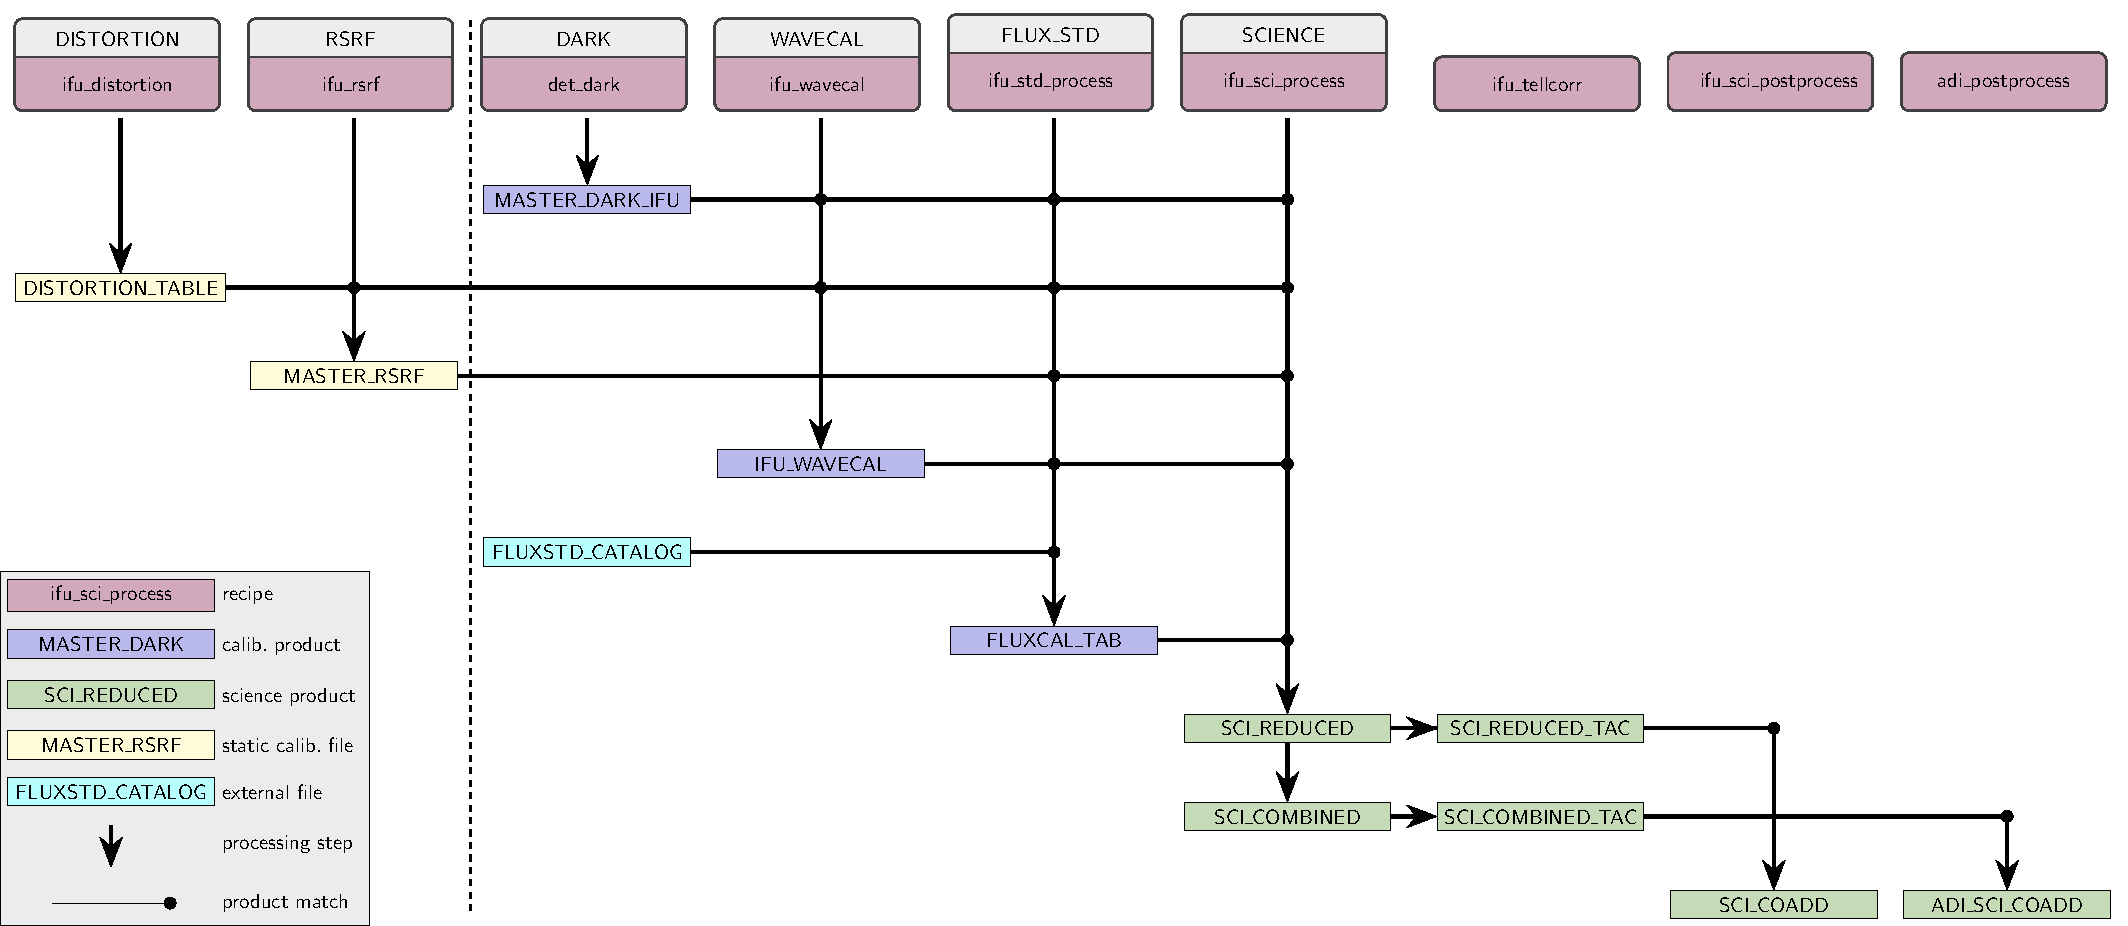
\includegraphics[width=\textheight]{IFU_assomap_tikz}
  \caption[Reduction cascade and association map for IFU
  spectroscopy]{%
    Association map for \ac{IFU} spectroscopy in L- and M-band. The
    figure shows only the primary products created by each recipe; for
    a full list of products refer to the recipe descriptions in
    Sect.~\ref{ssec:IFU_recipes}. The dashed line separates
    calibration tasks that are done at AIT or infrequently during
    operations from tasks done daily. The prefix ``\REC{metis_}'' has been
    omitted from the recipe names to improve clarity.}
  \label{Fig:IfuAssomap}
\end{sidewaysfigure}



%%%%%%%%%%%%%%%%%%%%%%%%%%%%%%%%%%%%%%%%%%%%%%%%%%%%%%

%%% Local Variables:
%%% TeX-master: "METIS_DRLD"
%%% End:


\subsection{Parallel Observing Modes}
\label{ssec:combinedmodes}

There are three parallel observing modes:

\begin{itemize}
\item Parallel observing mode IMG-LM and IMG-N (Section~\ref{sssec:parallellmnimg})
\item Parallel observing mode LSS-LM and LSS-N (Section~\ref{sssec:parallellmnspec})
\item Parallel observing mode IMG-LM and IFU (Section~\ref{sssec:parallellmnspec})
\end{itemize}

The respective templates corresponding to these modes will produce raw data files that can be processed independently by the relevant workflows.
That is, the templates will trigger two different recipe cascades, and there are no specific recipes for any of the parallel observing modes.

\subsubsection{Parallel observing mode IMG-LM and IMG-N}\label{sssec:parallellmnimg}
There are two specific templates for parallel imaging observations in the LM-band and N-band:
\begin{itemize}
 \item \TPL{METIS_img_lmn_obs_AutoChopNod}
 \item \TPL{METIS_img_lmn_obs_GenericChopNod}
\end{itemize}
These templates produce two kind of raw images that are processed independently in either the LM-band or N-band imaging workflow.
This fulfills \REQ{METIS-7244}.


\subsubsection{Parallel observing mode LSS-LM and LSS-N}\label{sssec:parallellmnspec}
There is one specific template for parallel LSS observations in the LM-band and N-band:
\begin{itemize}
 \item \TPL{METIS_spec_lmn_obs_AutoChopNodOnSlit}
\end{itemize}
These templates produce two kind of raw images that are processed independently in either the LM-band or N-band LSS workflow.
This fulfills \REQ{METIS-7245}.

\subsubsection{Parallel observing mode IMG-LM and IFU}\label{sssec:parallellmifu}
Parallel observing mode IMG-LM and IFU is also needed to perform non-common path pointing and aberration correction in \ac{HCI} modes:
real-time monitoring of non-common path aberrations between the \ac{SCAO} \ac{WFS} and the \ac{HCI} elements cannot be performed with the \ac{IFU} due to slicing and sampling issues.

The IFU pickoff optic is a beamsplitter with a transmission of ~10\% to the LM imager and a reflectivity of ~90\% to the IFU. % https://polarion.astron.nl/polarion/#/project/METIS/workitem?id=METIS-3111
LM-band images can therefore be taken in parallel with the IFU exposures, for any of the IFU templates.
The LM-band images and IFU exposures are processed independently.
This fulfills \REQ{METIS-6072}.


\subsection{Workflows}
The association matrices described in the previous sections will be converted one-to-one into Reflex or \ac{EDPS} workflows.

Any interactivity in the workflows is described with the individual recipes.


\subsection{Matched FITS keywords}

The workflow management system (e.g. \ac{EDPS}) uses the `matched keywords'
to find calibration data when processing data.
That is, the system will compare the FITS keywords of the primary input, to
the FITS headers of the pool of possible calibration files to use, in order
to decide what data to use.

For example, most calibration data has to be taken with the same \FITS{DET.DIT}
and \FITS{DET.NDIT} combination as the science data.
Several calibration products also need to use the same filter, or the same mask, or the same grism as the science data.

All selections are done on equality.
That is, no interpolation between, e.g., \FITS{DET.DIT}, will be done if only an approximate matching data product is found.

The following two tables provide an overview of the matched FITS
keywords. Table~\ref{tab:fitskeywordaliasses} defines several high level keyword
aliases used for convenience when there are several combinations
of instrumental keywords (INS.) which are needed to match with the correct
calibration files. These keywords are used in the Matched Keyword
descriptions in the recipes in Chapter~\ref{sec:pipeline_recipes}.
Table~\ref{tab:fitsmatchedkeywordssummary}
summaries the input data, calibration files, and the FITS
keyworlds needed to match them for all the recipes listed in
Chapter~\ref{sec:pipeline_recipes}. The second defines various high
level aliases used for convenience when there are several combinations
of instrumental keywords which are needed to match with the correct
calibration files.

\begin{table}
    \caption{FITS keyword aliases}
    \label{tab:fitskeywordaliasses}
  \begin{tabular}[c]{|p{3cm}|p{5cm}|p{5cm}|}
      \hline
      \textbf{Alias} & \textbf{Description} & \textbf{FITS keywords} \\
      \hline
\FITS{DRS.FILTER}   & Filter Information (LM or N)  & value of \FITS{INS.OPTI10.NAME} or \FITS{INS.OPTI13.NAME} \\
\FITS{DRS.NDFILTER} & ND Filter information	        & value of \FITS{INS.OPTI11.NAME} or \FITS{INS.OPTI13.NAME} \\
\FITS{DRS.SLIT}     & Slit Information (LM or N)    & value of \FITS{INS.OPTI3.NAME} and \FITS{INS.OPTI12.NAME} or  \FITS{INS.OPTI9.NAME} \\
\FITS{DRS.MASK}     & Mask information for Coronagraphy	& value of \FITS{INS.OPTI1.NAME}, \FITS{INS.OPTI3.NAME}, \FITS{INS.OPTI5.NAME}, \FITS{INS.OPTI9.NAME}, \FITS{INS.OPTI12.NAME} \\
\FITS{DRS.PUPIL}    & Pupil information             & value of \FITS{INS.OPTI15.NAME} or \FITS{INS.OPTI16.NAME}\\
\hline
    \end{tabular}
\end{table}


\newgeometry{bottom=0.1cm, right=0.1cm, left=0.1cm, top=0.1cm}
\begin{landscape}
{
  \begin{longtable}[c]{|p{4.2cm}|p{4.6cm}|p{5.6cm}|p{3.5cm}|p{3.5cm}|}
%  \begin{longtable}[c]{|l|l|l|l|l|}
 \caption{FITS matched keywords summary}
 \label{tab:fitsmatchedkeywordssummary}
 \endfirsthead
 \hline
 \textbf{Recipe} & \textbf{Main Input} & \textbf{Calibration Data} & \textbf{FITS keywords} & \textbf{Aliases} \\
 \hline
    \endhead
 \hline
 \textbf{Recipe} & \textbf{Main Input} & \textbf{Calibration Data} & \textbf{FITS keywords} & \textbf{Aliases} \\
 \hline
\REC{metis_det_lingain} & \RAW{DETLIN_det_RAW}, \RAW{det_WCU_OFF_RAW} &  &  &  \\
\REC{metis_det_dark} & \RAW{DARK_det_RAW} & \PROD{LINEARITY_det}, \PROD{PERSISTENCE_MAP} &  &  \\
\REC{metis_det_persistence} &  &  &  &  \\
\REC{metis_lm_img_flat} & \RAW{LM_FLAT_LAMP_RAW}, \RAW{LM_FLAT_TWILIGHT_RAW} & \PROD{MASTER_DARK_2RG} & \FITS{DET.DIT}, \FITS{DET.NDIT}, \FITS{INS.OPTI10.NAME} & \FITS{DET.DIT}, \FITS{DET.NDIT}, \FITS{DRS.FILTER},  \\
\REC{metis_lm_img_basic_reduce} & \RAW{LM_IMAGE_SCI_RAW} & \PROD{MASTER_DARK_2RG}, \PROD{MASTER_IMG_FLAT_LAMP_LM}, \PROD{MASTER_IMG_FLAT_TWILIGHT_LM} & \FITS{DET.DIT}, \FITS{DET.NDIT}, \FITS{INS.OPTI10.NAME} & \FITS{DET.DIT}, \FITS{DET.NDIT}, \FITS{DRS.FILTER},  \\
\REC{metis_lm_img_background} & \RAW{LM_SCI_BASIC_REDUCED}, \RAW{LM_STD_BASIC_REDUCED} &  & \FITS{INS.OPTI10.NAME} & \FITS{DRS.FILTER},  \\
\REC{metis_lm_img_std_process} & \RAW{LM_STD_BKG_SUBTRACTED} & \PROD{FLUXSTD_CATALOG} & \FITS{INS.OPTI10.NAME} & \FITS{DRS.FILTER},  \\
\REC{metis_lm_img_calibrate} & \RAW{LM_SCI_BKG_SUBTRACTED} & \PROD{FLUXCAL_TAB}, \PROD{LM_DISTORTION_TABLE} & \FITS{INS.OPTI10.NAME} & \FITS{DRS.FILTER},  \\
\REC{metis_lm_img_sci_postprocess} & \RAW{LM_SCI_CALIBRATED} &  & \FITS{INS.OPTI10.NAME} & \FITS{DRS.FILTER},  \\
\REC{metis_lm_img_distortion} & \RAW{LM_DISTORTION_RAW}, \RAW{LM_WCU_OFF_RAW} & \EXTCALIB{PINHOLE_TABLE} & \FITS{INS.OPTI10.NAME} & \FITS{DRS.FILTER},  \\
\REC{metis_n_img_flat} & \RAW{N_FLAT_LAMP_RAW}, \RAW{N_FLAT_TWILIGHT_RAW} & \PROD{MASTER_DARK_GEO} & \FITS{DET.DIT}, \FITS{DET.NDIT}, \FITS{INS.OPTI10.NAME} & \FITS{DET.DIT}, \FITS{DET.NDIT}, \FITS{DRS.FILTER},  \\
\REC{metis_n_img_chopnod} & \RAW{N_IMAGE_SCI_RAW} & \PROD{N_FLAT_LAMP_RAW}, \PROD{N_FLAT_TWILIGHT_RAW} & \FITS{DET.DIT}, \FITS{DET.NDIT}, \FITS{INS.OPTI10.NAME} & \FITS{DET.DIT}, \FITS{DET.NDIT}, \FITS{DRS.FILTER},  \\
\REC{metis_n_img_std_process} & \RAW{N_STD_BKG_SUBTRACTED} & \PROD{FLUXSTD_CATALOG} & \FITS{INS.OPTI13.NAME} & \FITS{DRS.FILTER},  \\
\REC{metis_n_img_calibrate} & \RAW{N_SCI_BKG_SUBTRACTED} & \PROD{FLUXCAL_TAB}, \PROD{N_DISTORTION_TABLE} & \FITS{INS.OPTI13.NAME} & \FITS{DRS.FILTER},  \\
\REC{metis_n_img_restore} & \RAW{N_SCI_CALIBRATED} &  & \FITS{INS.OPTI13.NAME} & \FITS{DRS.FILTER},  \\
\REC{metis_n_img_distortion} & \RAW{N_DISTORTION_RAW}, \RAW{N_WCU_OFF_RAW} & \EXTCALIB{PINHOLE_TABLE} & \FITS{INS.OPTI13.NAME} & \FITS{DRS.FILTER},  \\
\REC{metis_lm_lss_rsrf} & \RAW{LM_LSS_RSRF_RAW}, \RAW{LM_WCU_OFF_RAW} & \PROD{LINEARITY_2RG}, \PROD{PERSISTENCE_MAP}, \PROD{GAIN_MAP_2RG}, \PROD{MASTER_DARK_2RG} & \FITS{DET.DIT}, \FITS{DET.NDIT}, \FITS{INS.OPTI9.NAME} & \FITS{DET.DIT}, \FITS{DET.NDIT}, \FITS{DRS.SLIT},  \\
\REC{metis_lm_lss_trace} & \RAW{LM_LSS_RSRF_PINH_RAW}, \RAW{LM_WCU_OFF_RAW} & \PROD{LINEARITY_2RG}, \PROD{PERSISTENCE_MAP}, \PROD{GAIN_MAP_2RG}, \PROD{MASTER_DARK_2RG}, \PROD{MASTER_LM_LSS_RSRF} & \FITS{DET.DIT}, \FITS{DET.NDIT}, \FITS{INS.OPTI9.NAME} & \FITS{DET.DIT}, \FITS{DET.NDIT}, \FITS{DRS.SLIT},  \\
\REC{metis_lm_lss_wave} & \RAW{LM_LSS_WAVE_RAW} & \PROD{LINEARITY_2RG}, \PROD{PERSISTENCE_MAP}, \PROD{GAIN_MAP_2RG}, \PROD{MASTER_DARK_2RG}, \PROD{MASTER_LM_LSS_RSRF}, \PROD{LM_LSS_TRACE}, \PROD{LASER_TAB} & \FITS{DET.DIT}, \FITS{DET.NDIT}, \FITS{INS.OPTI9.NAME}, \FITS{SEQ.WCU.LASERn} & \FITS{DET.DIT}, \FITS{DET.NDIT}, \FITS{DRS.SLIT}, \FITS{SEQ.WCU.LASERn},  \\
\REC{metis_lm_lss_std} & \RAW{LM_LSS_STD_RAW} & \PROD{LINEARITY_2RG}, \PROD{PERSISTENCE_MAP}, \PROD{GAIN_MAP_2RG}, \PROD{MASTER_DARK_2RG}, \PROD{MASTER_LM_LSS_RSRF}, \PROD{LM_LSS_DIST_SOL}, \PROD{LM_LSS_WAVE_GUESS}, \PROD{AO_PSF_MODEL}, \PROD{ATM_LINE_CAT}, \PROD{LM_ADC_SLITLOSS}, \PROD{LM_SYNTH_TRANS}, \PROD{REF_STD_CAT} & \FITS{DET.DIT}, \FITS{DET.NDIT}, \FITS{INS.OPTI9.NAME} & \FITS{DET.DIT}, \FITS{DET.NDIT}, \FITS{DRS.SLIT},  \\
\REC{metis_n_lss_sci} & \RAW{LM_LSS_SCI_RAW} & \PROD{LINEARITY_2RG}, \PROD{PERSISTENCE_MAP}, \PROD{GAIN_MAP_2RG}, \PROD{MASTER_DARK_2RG}, \PROD{MASTER_LM_LSS_RSRF}, \PROD{LM_LSS_DIST_SOL}, \PROD{LM_LSS_WAVE_GUESS}, \PROD{AO_PSF_MODEL}, \PROD{ATM_LINE_CAT}, \PROD{LM_ADC_SLITLOSS}, \PROD{STD_TRANSMISSION}, \PROD{MASTER_LM_RESPONSE} & \FITS{DET.DIT}, \FITS{DET.NDIT}, \FITS{INS.OPTI9.NAME} & \FITS{DET.DIT}, \FITS{DET.NDIT}, \FITS{DRS.SLIT},  \\
\REC{metis_lm_lss_mf_model} & \RAW{LM_LSS_SCI_FLUX_1D} & \PROD{LSF_KERNEL}, \PROD{ATM_PROFILE}, \PROD{ATM_LINE_CAT} & \FITS{INS.OPTI9.NAME} & \FITS{DRS.SLIT},  \\
\REC{metis_lm_lss_mf_calctrans} & \RAW{MF_BEST_FIT_TAB} & \PROD{LSF_KERNEL}, \PROD{ATM_PROFILE}, \PROD{ATM_LINE_CAT} & \FITS{INS.OPTI9.NAME} & \FITS{DRS.SLIT},  \\
\REC{metis_lm_lss_mf_correct} & \RAW{LM_LSS_SCI_FLUX_1D}, \RAW{LM_LSS_SYNTH_TRANS} &  & \FITS{INS.OPTI9.NAME} & \FITS{DRS.SLIT},  \\
\REC{metis_n_lss_rsrf} & \RAW{N_LSS_RSRF_RAW}, \RAW{N_WCU_OFF_RAW} & \PROD{LINEARITY_GEO}, \PROD{PERSISTENCE_MAP}, \PROD{GAIN_MAP_GEO}, \PROD{MASTER_DARK_GEO} & \FITS{DET.DIT}, \FITS{DET.NDIT}, \FITS{INS.OPTI12.NAME} & \FITS{DET.DIT}, \FITS{DET.NDIT}, \FITS{DRS.SLIT},  \\
\REC{metis_n_lss_trace} & \RAW{N_LSS_RSRF_PINH_RAW}, \RAW{N_WCU_OFF_RAW} & \PROD{LINEARITY_GEO}, \PROD{PERSISTENCE_MAP}, \PROD{GAIN_MAP_GEO}, \PROD{MASTER_DARK_GEO}, \PROD{MASTER_N_LSS_RSRF} & \FITS{DET.DIT}, \FITS{DET.NDIT}, \FITS{INS.OPTI12.NAME} & \FITS{DET.DIT}, \FITS{DET.NDIT}, \FITS{DRS.SLIT},  \\
%\REC{metis_n_lss_wave} & \RAW{N_LSS_WAVE_RAW} & \PROD{LINEARITY_GEO}, \PROD{PERSISTENCE_MAP}, \PROD{GAIN_MAP_GEO}, \PROD{MASTER_DARK_GEO}, \PROD{MASTER_N_LSS_RSRF}, \PROD{N_LSS_TRACE}, \PROD{LASER_TAB} & \FITS{DET.DIT}, \FITS{DET.NDIT}, \FITS{INS.OPTI12.NAME}, \FITS{SEQ.WCU.LASERn} & \FITS{DET.DIT}, \FITS{DET.NDIT}, \FITS{DRS.SLIT}, \FITS{SEQ.WCU.LASERn},  \\
\REC{metis_n_lss_std} & \RAW{N_LSS_STD_RAW} & \PROD{LINEARITY_GEO}, \PROD{PERSISTENCE_MAP}, \PROD{GAIN_MAP_GEO}, \PROD{MASTER_DARK_GEO}, \PROD{MASTER_N_LSS_RSRF}, \PROD{N_LSS_DIST_SOL}, \PROD{N_LSS_WAVE_GUESS}, \PROD{AO_PSF_MODEL}, \PROD{ATM_LINE_CAT}, \PROD{N_ADC_SLITLOSS}, \PROD{N_SYNTH_TRANS}, \PROD{REF_STD_CAT} & \FITS{DET.DIT}, \FITS{DET.NDIT}, \FITS{INS.OPTI12.NAME} & \FITS{DET.DIT}, \FITS{DET.NDIT}, \FITS{DRS.SLIT},  \\
\REC{metis_n_lss_sci} & \RAW{N_LSS_SCI_RAW} & \PROD{LINEARITY_GEO}, \PROD{PERSISTENCE_MAP}, \PROD{GAIN_MAP_GEO}, \PROD{MASTER_DARK_GEO}, \PROD{MASTER_N_LSS_RSRF}, \PROD{N_LSS_DIST_SOL}, \PROD{N_LSS_WAVE_GUESS}, \PROD{AO_PSF_MODEL}, \PROD{ATM_LINE_CAT}, \PROD{N_ADC_SLITLOSS}, \PROD{STD_TRANSMISSION}, \PROD{MASTER_N_RESPONSE} & \FITS{DET.DIT}, \FITS{DET.NDIT}, \FITS{INS.OPTI12.NAME} & \FITS{DET.DIT}, \FITS{DET.NDIT}, \FITS{DRS.SLIT},  \\
\REC{metis_n_lss_mf_model} & \RAW{N_LSS_SCI_FLUX_1D} & \PROD{LSF_KERNEL}, \PROD{ATM_PROFILE}, \PROD{ATM_LINE_CAT} & \FITS{INS.OPTI12.NAME} & \FITS{DRS.SLIT},  \\
\REC{metis_n_lss_mf_calctrans} & \RAW{MF_BEST_FIT_TAB} & \PROD{LSF_KERNEL}, \PROD{ATM_PROFILE}, \PROD{ATM_LINE_CAT} & \FITS{INS.OPTI12.NAME} & \FITS{DRS.SLIT},  \\
\REC{metis_n_lss_mf_correct} & \RAW{N_LSS_SCI_FLUX_1D}, \RAW{N_LSS_SYNTH_TRANS} &  & \FITS{INS.OPTI12.NAME} & \FITS{DRS.SLIT},  \\
\REC{metis_ifu_wavecal} & \RAW{IFU_WAVE_RAW} & \PROD{MASTER_DARK_IFU}, \PROD{IFU_DISTORTION_TABLE} & \FITS{DET.DIT}, \FITS{DET.NDIT}, \FITS{INS.OPTI6.NAME} & \FITS{DET.DIT}, \FITS{DET.NDIT}, \FITS{DRS.IFU},  \\
\REC{metis_ifu_rsrf} & \RAW{IFU_RSRF_RAW} & \PROD{MASTER_DARK_IFU}, \PROD{IFU_WAVECAL} & \FITS{DET.DIT}, \FITS{DET.NDIT}, \FITS{INS.OPTI6.NAME} & \FITS{DET.DIT}, \FITS{DET.NDIT}, \FITS{DRS.IFU},  \\
\REC{metis_ifu_calibrate} & \RAW{IFU_STD_RAW} & \PROD{MASTER_DARK_IFU}, \PROD{RSRF_IFU}, \PROD{IFU_WAVECAL}, \PROD{IFU_DISTORTION_TABLE} & \FITS{DET.DIT}, \FITS{DET.NDIT}, \FITS{INS.OPTI6.NAME} & \FITS{DET.DIT}, \FITS{DET.NDIT}, \FITS{DRS.IFU},  \\
\REC{metis_ifu_telluric} & \RAW{IFU_SCI_COMBINED} & \PROD{LSF_KERNEL}, \PROD{ATM_PROFILE} & \FITS{DET.DIT}, \FITS{DET.NDIT}, \FITS{INS.OPTI6.NAME} & \FITS{DET.DIT}, \FITS{DET.NDIT}, \FITS{DRS.IFU},  \\
\REC{metis_ifu_calibrate} & \RAW{IFU_SCI_REDUCED}, \PROD{FLUXCAL_TAB} &  & \FITS{INS.OPTI6.NAME} & \FITS{DRS.IFU},  \\
\REC{metis_ifu_postprocess} & \RAW{IFU_SCI_REDUCED} &  & \FITS{INS.OPTI6.NAME} & \FITS{DRS.IFU},  \\
\REC{metis_ifu_distortion} & \RAW{IFU_DISTORTION_RAW} & \EXTCALIB{PINHOLE_TABLE} & \FITS{INS.OPTI6.NAME} & \FITS{DRS.IFU},  \\
\REC{metis_img_adi_cgrph} & \RAW{LM_SCI_BASIC_REDUCED}, \RAW{N_SCI_BKG_SUBTRACTED} & \PROD{LM_DISTORTION_TABLE}, \PROD{N_DISTORTION_TABLE}, \PROD{LM_cgrph_SCI_THROUGHPUT}, \PROD{N_cgrph_SCI_THROUGHPUT} & \FITS{INS.OPTI1.NAME}, \FITS{INS.OPTI3.NAME}, \FITS{INS.OPTI5.NAME}, \FITS{INS.OPTI9.NAME}, \FITS{INS.OPTI10.NAME}, \FITS{INS.OPTI13.NAME} & \FITS{DRS.MASK},  \\
\REC{metis_lm_adi_app} & \RAW{LM_SCI_BASIC_REDUCED} & \PROD{LM_DISTORTION_TABLE}, \PROD{LM_OFF_AXIS_PSF_RAW} & \FITS{INS.OPTI5.NAME}, \FITS{INS.OPTI9.NAME}, \FITS{INS.OPTI10.NAME} & \FITS{DRS.MASK},  \\
\REC{metis_ifu_adi_cgrph} & \RAW{IFU_SCI_REDUCED} & \PROD{IFU_DISTORTION_TABLE}, \PROD{IFU_cgrph_SCI_THROUGHPUT} & \FITS{INS.OPTI6.NAME}, \FITS{INS.OPTI1.NAME}, \FITS{INS.OPTI3.NAME}, \FITS{INS.OPTI5.NAME}, \FITS{INS.OPTI9.NAME}, \FITS{INS.OPTI12.NAME} & \FITS{DRS.MASK},  \\
\REC{metis_pupil_imaging} & \RAW{LM_PUPIL_RAW}, \RAW{N_PUPIL_RAW} &  & \FITS{INS.OPTI15.NAME}, \FITS{INS.OPTI16.NAME}, \FITS{INS.OPTI10.NAME}, \FITS{INS.OPTI13.NAME} & \FITS{DRS.PUPIL},  \\
\REC{metis_cal_chophome} & \RAW{LM_CHOPHOME_RAW} & \PROD{LINEARITY_2RG}, \PROD{PERSISTENCE_MAP}, \PROD{GAIN_MAP_2RG}, \PROD{MASTER_DARK_2RG}, \PROD{MASTER_IMG_FLAT_LAMP_LM} & \FITS{DET.DIT}, \FITS{DET.NDIT}, \FITS{INS.OPTI10.NAME} & \FITS{DET.DIT}, \FITS{DET.NDIT}, \FITS{DRS.FILTER},  \\
\REC{metis_lm_adc_slitloss} & \RAW{LM_SLITLOSSES_RAW}, \RAW{LM_WCU_OFF_RAW} & \PROD{LINEARITY_2RG}, \PROD{PERSISTENCE_MAP}, \PROD{GAIN_MAP_2RG}, \PROD{MASTER_DARK_2RG}, \PROD{MASTER_IMG_FLAT_LAMP_LM} & \FITS{INS.OPTI10.NAME}, \FITS{INS.OPTI13.NAME} & \FITS{DET.DIT}, \FITS{DET.NDIT}, \FITS{DRS.FILTER},  \\
\REC{metis_n_adc_slitloss} & \RAW{LM_SLITLOSSES_RAW}, \RAW{LM_WCU_OFF_RAW} & \PROD{LINEARITY_GEO}, \PROD{PERSISTENCE_MAP}, \PROD{GAIN_MAP_GEO}, \PROD{MASTER_DARK_GEO}, \PROD{MASTER_IMG_FLAT_LAMP_N} & \FITS{INS.OPTI10.NAME}, \FITS{INS.OPTI13.NAME} & \FITS{DET.DIT}, \FITS{DET.NDIT}, \FITS{DRS.FILTER},  \\
    \hline
    \end{longtable}
  }
\end{landscape}
\restoregeometry

%%% Local Variables:
%%% TeX-master: "METIS_DRLD"
%%% End:


% Imaging-mode
% \input{05_1-Overview_Imaging}

% LSS-mode
% \subsection{Long-Slit Spectroscopy in L/M- and N-bands}\label{lss:overview}
\subsubsection{The workflow cascades}\label{lss:cascade_overview}
The purpose of the pipeline is to correct or remove contributions from
the instrument, telescope, and atmosphere and generate science-grade
data products for the L/M- and N-band \ac{LSS}
mode. Since the detector properties are not fully specified, especially of the new Geosnap, we currently assume
basically the same reduction cascade for both spectral ranges LM and
N, respectively. The only major difference at the time being is the absence of \ac{WCU} laser sources in the N-band, which are only available during \ac{AIT} phase to generate a first guess of the pixel-to-wavelength relation. Therefore the first guess wavelength solution in the N-band will be based on that \ac{AIT} data. As we assume the instrument to be very stable, that approach should be sufficient for the low-resolution N-band spectroscopy. In the LM range, two fix-frequency lasers ($@3.39$µm and $@5.26$µm) and one tuneable ($4.68....4.78$µm) is foreseen in the \ac{WCU} to be taken on daily basis (cf. \cite{METIS-calibration_plan}). Although mainly foreseen to be used for the high-resolution spectroscopy \ac{LMS} mode, we can use these laser sources for the LM-band \ac{LSS} as well.

Special emphasis has to be drawn to the effects of the Earth's
atmosphere in several respects:
\begin{itemize}
\item Wavelength calibration: Absorption/emission features are intended to be
  used for the wavelength calibration. Thus, a good knowledge on /
  identification of these features is crucial for the accuracy of the
  wavelength calibration.
\item Telluric correction: In the MIR regime telluric absorption is
  one of the most dominant effects visible in spectra. Modelling
  approaches like \texttt{molecfit} heavily rely on accurate
  atmospheric input profiles, which represent the actual state and
  composition of the Earth's atmosphere. This especially applies to
  the \ac{PWV} content since this is the most
  dominant and most variable species.
\item Atmospheric dispersion: \ac{METIS} will have \ac{ADC}s compensating the
  effect of atmospheric dispersion. However, for technical reasons
  these ADCs are fixed at several positions. This means that the
  compensation is only partially. This leads to two practical effects:
  (a) wavelength-dependent slit losses, and (b) distortions in both,
  the spatial and the spectral direction (see \cite{METIS-ADC_study}
  for more details). For both, the pipeline needs to correct
  for. It is foreseen to determine these slitlosses on yearly basis with a separate calibration task (cf. \cite{METIS-calibration_plan}) and create a slit-loss table to be included in the static calibration database.
\end{itemize}

%However, to keep flexibility and independence of both branches, we
%define different recipes for the time being, although they will be
%mostly based on the same algorithms. We therefore focus here on the LM-band only.

Figures~\ref{Fig:LMLssAssomap1} and \ref{Fig:LMLssAssomap2} show the reduction cascade and the association map for the recipes handling L/M-long-slit
spectroscopy data.  Table~\ref{Tab:LMLssDatProc} contains the data processing table for this mode. For the N-band \ac{LSS} mode the cascade and the data processing table is given in Fig.\ref{Fig:NLssAssomap} and Table~\ref{Tab:NLssDatProc}, respectively (cf. also Fig.~\ref{Fig:LSScascadelegend}).

In general, there are four major steps in each of the two cascades:
\begin{itemize}
    \item \textbf{Preparation step:} This contains the recipes, which are invoked only rarely, e.g. after major instrument interventions, or on monthly/yearly basis to update the static calibration database. These recipes are therefore not shown in the cascade in Figs.~\ref{Fig:LMLssAssomap1}/\ref{Fig:LMLssAssomap2} and \ref{Fig:NLssAssomap} and the corresponding data processing tables. In case of the \ac{LSS} pipeline this concerns the creation of the gain maps/linearity checks (see Section~\ref{sssec:metis_det_lingain}), the determination of the slit losses induced by the fixed positions of the ADCs (cf. Section~\ref{sssec:adc_slitlosses} and Section "Calibration of slit losses" in Calibration plan \cite{METIS-calibration_plan}) and the zero position of the chopping mirror (see Section~\ref{ssec:metisimgchophome} and Section "Chopper Home Position" in \cite{METIS-calibration_plan} for more details). T
    \item \textbf{Basic steps}: The basic steps aim for correcting the detector influence, in particular the dark correction and the determination of the master \ac{RSRF}.
    \item \textbf{Calibration/correction steps}: This is the main part which incorporates the order trace detection, distortion, wavelength and flux correction.
    \item \textbf{Post-calibration steps}: After havig calibrated spectra at hand, the last step is the telluric absorption correction.
\end{itemize}

\begin{figure}[ht]
  \centering
  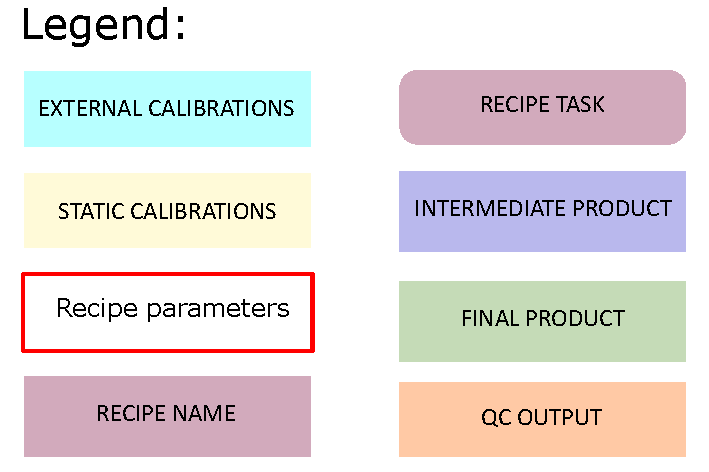
\includegraphics[width=0.4\textheight]{figures/legend.pdf}
  \caption[Legend]{Legend of the coloured boxes in the \ac{LSS} cascades.}
  \label{Fig:LSScascadelegend}
\end{figure}
\clearpage

\begin{sidewaysfigure}[ht]
  \centering
  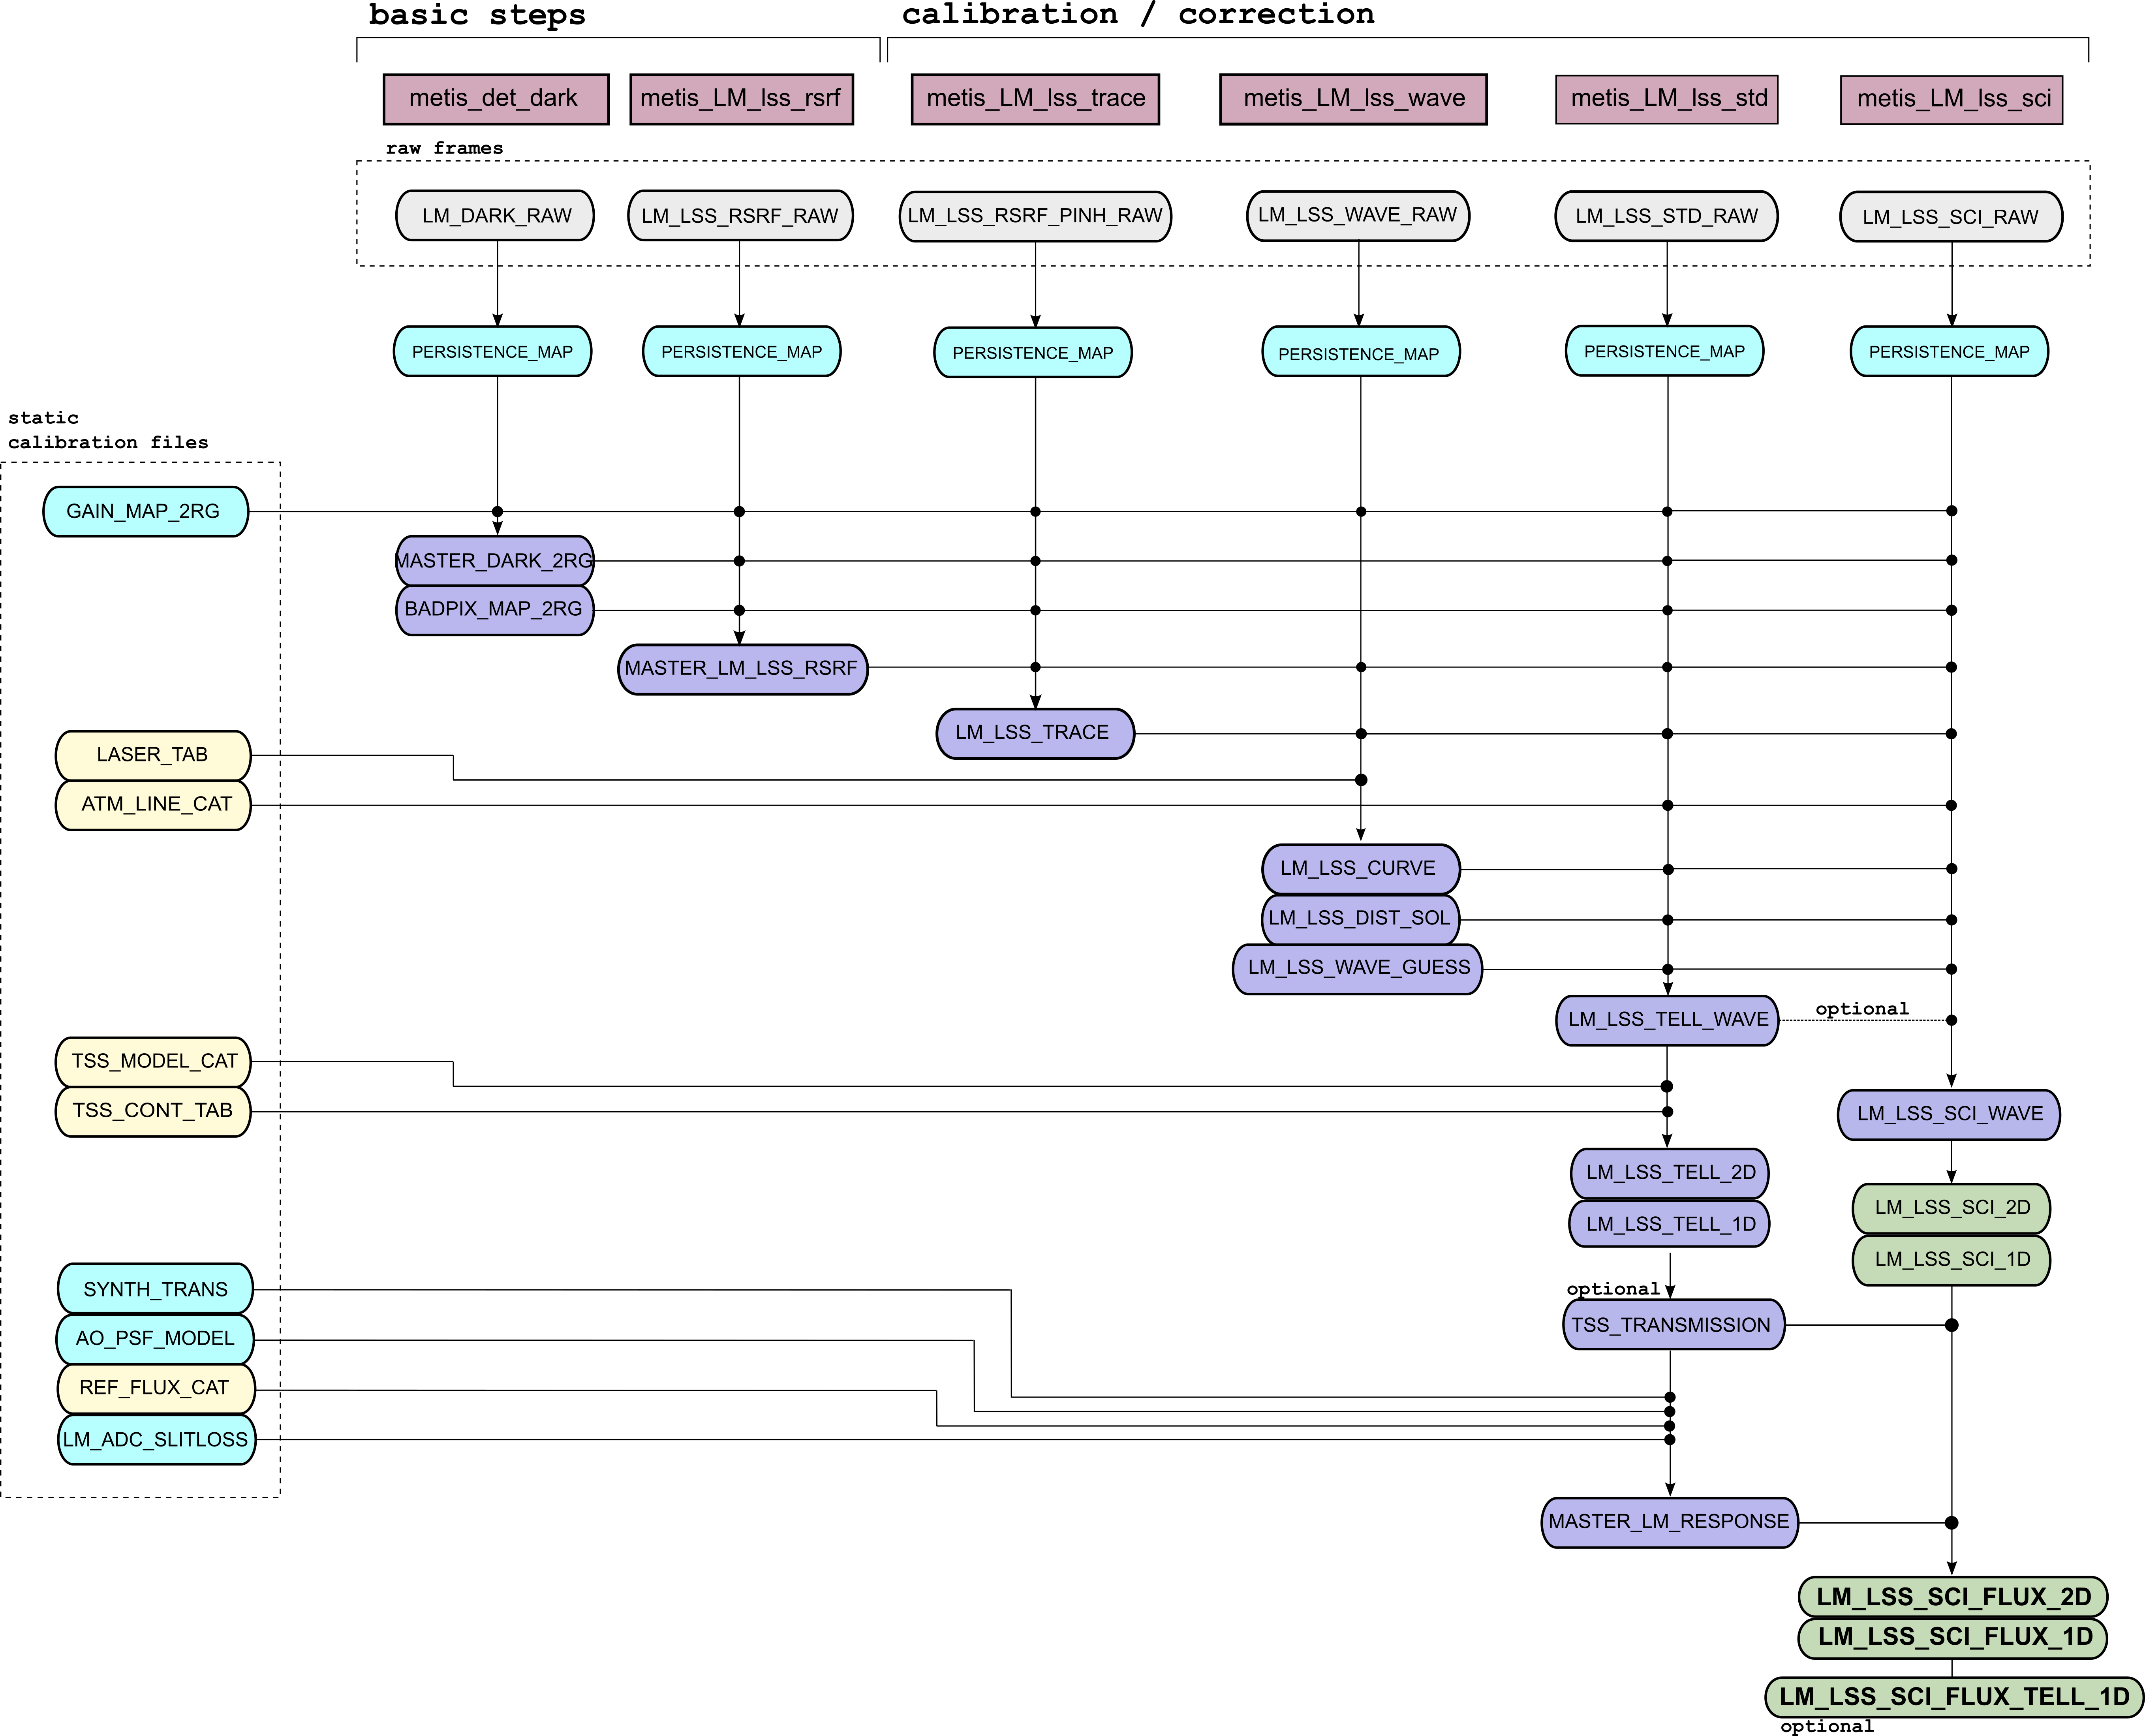
\includegraphics[width=0.9\textheight]{figures/LM_LSS_pipeline_wf_draft_latest_part_1_v0.80.png}
  \caption[Reduction cascade and association map for LM long-slit
  spectroscopy]{Part 1 of the reduction cascade and association map for long-slit
    spectroscopy in the LM bands.  }
  \label{Fig:LMLssAssomap1}
\end{sidewaysfigure}

\begin{sidewaysfigure}[ht]
  \centering
  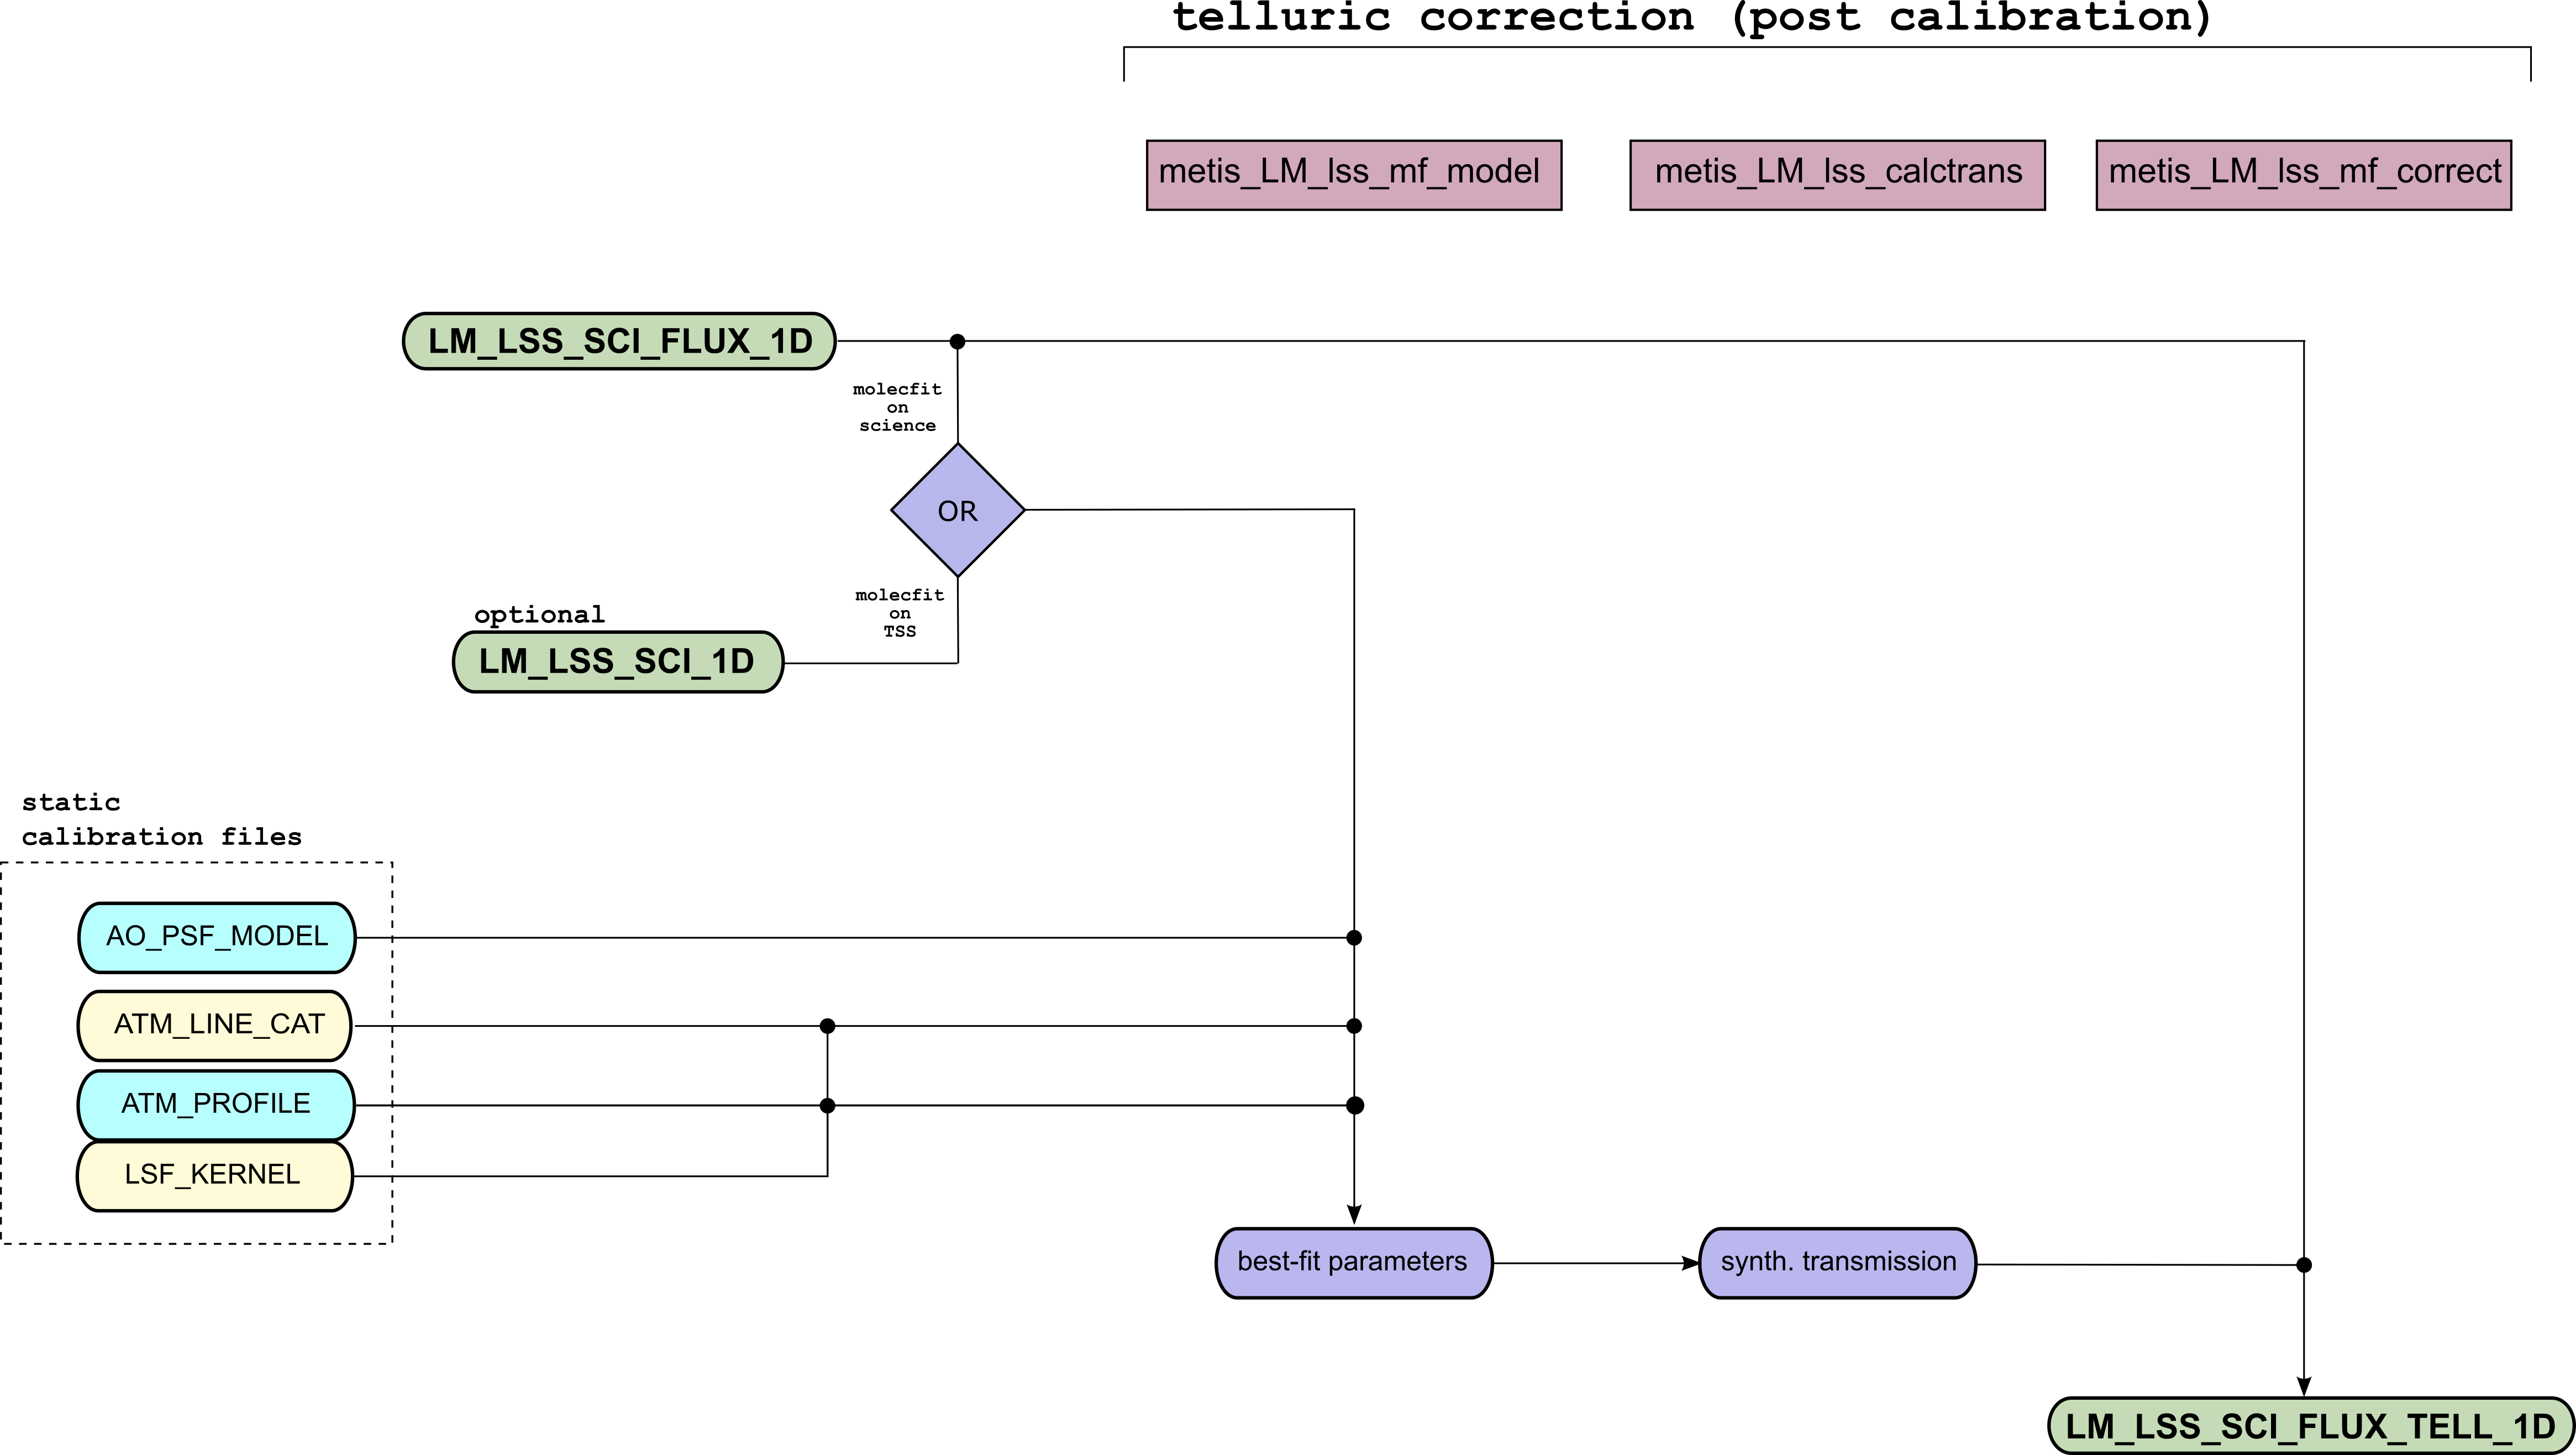
\includegraphics[width=0.8\textheight]{figures/LM_LSS_pipeline_wf_draft_latest_part_2_v0.80.png}
  \caption[Reduction cascade and association map for LM long-slit
  spectroscopy]{Part 2 of the reduction cascade and association map for long-slit
    spectroscopy in the LM bands.  }
  \label{Fig:LMLssAssomap2}
\end{sidewaysfigure}


% \begin{sidewaysfigure}[ht]
%   \centering
%   \includegraphics[width=0.9\textheight]{figures/NQ_LSS_pipeline_wf_draft_latest.png}
%   \caption[Reduction cascade and association map for N long-slit
%   spectroscopy]{Reduction cascade and association map for long-slit
%     spectroscopy in the N band.  }
%   \label{Fig:NQLssAssomap}
% \end{sidewaysfigure}


%% ---- Table: LM long-slit spectroscopy
\begin{sidewaystable}
  \footnotesize
  \begin{center}
    \caption[Data Processing table for LM long-slit spectroscopy]{%
      Data Processing table for LM long-slit spectroscopy
      calibration mode; }\bigskip
    \label{Tab:LMLssDatProc}
    \begin{tabular}{|l|l|l|l|l|l|}
      \hline
      Data Type   & Classification & Recipe (Level)	& FITS Keywords & static CalibDB & Products\\
    (Templates) & Keywords	 & Processing steps	&		&	  &	\\
    \hline
    \TPL{DARK}	& \CODE{DPR.CATG==CALIB} & \hyperref[sssec:metis_det_dark]{\REC{metis_det_dark}} & Exposure time	&	\hyperref[dataitem:gainmap2rg]{\PROD{GAIN_MAP_2RG}}& Averaged dark frame\\
    		& \CODE{DPR.TYPE==DARK}  &			&		&	& Bad pixel map\\
    		& \CODE{DPR.TECH==IMAGE}  &			&		&	& \\
    \hline
    \TPL{FLAT}	& \CODE{DPR.CATG==CALIB} & \hyperref[rec:lsslmrsrf]{\REC{metis_LM_lss_rsrf}} & Exposure time	& \hyperref[dataitem:gainmap2rg]{\PROD{GAIN_MAP_2RG}}	& Averaged, normalized flatfield\\
    		& \CODE{DPR.TYPE==FLAT}  &			&	Grism	& 	& \\
    		& \CODE{DPR.TECH==SPECTRUM}  &			&	Slit	&	& \\
    \hline
         	& \CODE{DPR.CATG==CALIB} &\hyperref[rec:lsslmtrace]{\REC{metis_LM_lss_trace}} & Exposure time	& \hyperref[dataitem:gainmap2rg]{\PROD{GAIN_MAP_2RG}}	& Order location\\
    		& \CODE{DPR.TYPE==FLAT}  &			&		&	& (polynomial fit)\\
    		& \CODE{DPR.TECH==SPECTRUM}  &			&		&	& \\
    \hline
    \TPL{WAVE,LASER} & \CODE{DPR.CATG==CATG} &\hyperref[rec:lsslmwave]{\REC{metis_LM_lss_wave}} & Exposure time &  \hyperref[dataitem:gainmap2rg]{\PROD{GAIN_MAP_2RG}} & wavelength solution\\
    		& \CODE{DPR.TYPE==WAVE,LASER}   &			   & Grism & \hyperref[dataitem:lasertab]{\STATCALIB{LASER_TAB}} &\\
    		& \CODE{DPR.TECH==SPECTRUM}  &			& Slit		&	& \\
    		& \CODE{PRO.CATG==SPECTRUM}   &  &  & & \\
    \hline
    \TPL{FLUX,STD} & \CODE{DPR.CATG==CALIB} & \hyperref[rec:lsslmstd]{\REC{metis_LM_lss_flux}}& Object name (Flux STD) & \hyperref[dataitem:gainmap2rg]{\PROD{GAIN_MAP_2RG}} & Instrumental\\
    		& \CODE{DPR.TYPE==FLUX,STD}   &			   & Exposure time & \hyperref[dataitem:atmlinecat]{\EXTCALIB{ATM_LINE_CAT}} & response function\\
    		& \CODE{DPR.TECH==SPECTRUM}  &			&	Grism	&	\hyperref[dataitem:lmsynthtrans]{\STATCALIB{LM_SYNTH_TRANS}}& \\
    		& \CODE{PRO.CATG==SPECTRUM}   &  & Slit & \hyperref[dataitem:lmadcslitloss]{\STATCALIB{LM_ADC_SLITLOSS}} & \\
    		& & & & \hyperref[dataitem:aopsfmodel]{\EXTCALIB{AO_PSF_MODEL}} &\\    
    		& & & & \hyperref[dataitem:reffluxcat]{\STATCALIB{REF_FLUX_CAT}} &\\    \hline
    \TPL{SCIENCE} & \CODE{DPR.CATG==SCIENCE} & \hyperref[rec:lsslmsci]{\REC{metis_LM_lss_sci}} & Object name &  \hyperref[dataitem:gainmap2rg]{\PROD{GAIN_MAP_2RG}} & Science grade spectrum\\
    		& \CODE{DPR.TYPE==OBJECT}   &			   & Exposure time & \hyperref[dataitem:lmadcslitloss]{\STATCALIB{LM_ADC_SLITLOSS}} &\\
    		& \CODE{DPR.TECH==SPECTRUM}  &			&	Grism	& \hyperref[dataitem:atmlinecat]{\EXTCALIB{ATM_LINE_CAT}}	& \\
    		& \CODE{PRO.CATG==SPECTRUM}   &  & Slit  &  & \\
    \hline
            & \CODE{DPR.CATG==SCIENCE} & \hyperref[rec:LMLSSmfmodel]{\REC{metis_LM_lss_mf_model}} & Object name & \hyperref[dataitem:lsfkernel]{\STATCALIB{LSF_KERNEL}}	 & Best-fit \\
    		& \CODE{DPR.TYPE==OBJECT}   &			  & & \hyperref[dataitem:atmprofile]{\EXTCALIB{ATM_PROFILE}}  & \texttt{molecfit} parameters\\
    		& \CODE{DPR.TECH==TBD}  &			&		& \hyperref[dataitem:atmlinecat]{\EXTCALIB{ATM_LINE_CAT}}	& \\
    		& \CODE{PRO.CATG==TBD}   &  &  & start parameter set & \\
    \hline
            & \CODE{DPR.CATG==SCIENCE} &  \hyperref[rec:LMLSSmfcalctrans]{\REC{metis_LM_lss_mf_calctrans}} & Object name & \hyperref[dataitem:atmlinecat]{\EXTCALIB{ATM_LINE_CAT}}	 & synthetic \\
    		& \CODE{DPR.TYPE==LSS}   &		&	   &   & Transmission curve\\
    		& \CODE{DPR.TECH==TBD}  &			&		& 	& \\
    		& \CODE{PRO.CATG==TBD}   &  &  & & \\
    \hline
            & \CODE{DPR.CATG==SCIENCE} &  \hyperref[rec:LMLSSmfcorrect]{\REC{metis_LM_lss_mf_correct}} & Object name & 	 & Absorption corrected\\
    		& \CODE{DPR.TYPE==LSS}   &			   & & synthetic Transmission curve  & science spectrum\\
    		& \CODE{DPR.TECH==TBD}  &			&		&	& \\
    		& \CODE{PRO.CATG==TBD}   &  &  & & \\
    \hline
    \end{tabular}
  \end{center}
\end{sidewaystable}

\begin{sidewaysfigure}[ht]
  \centering
  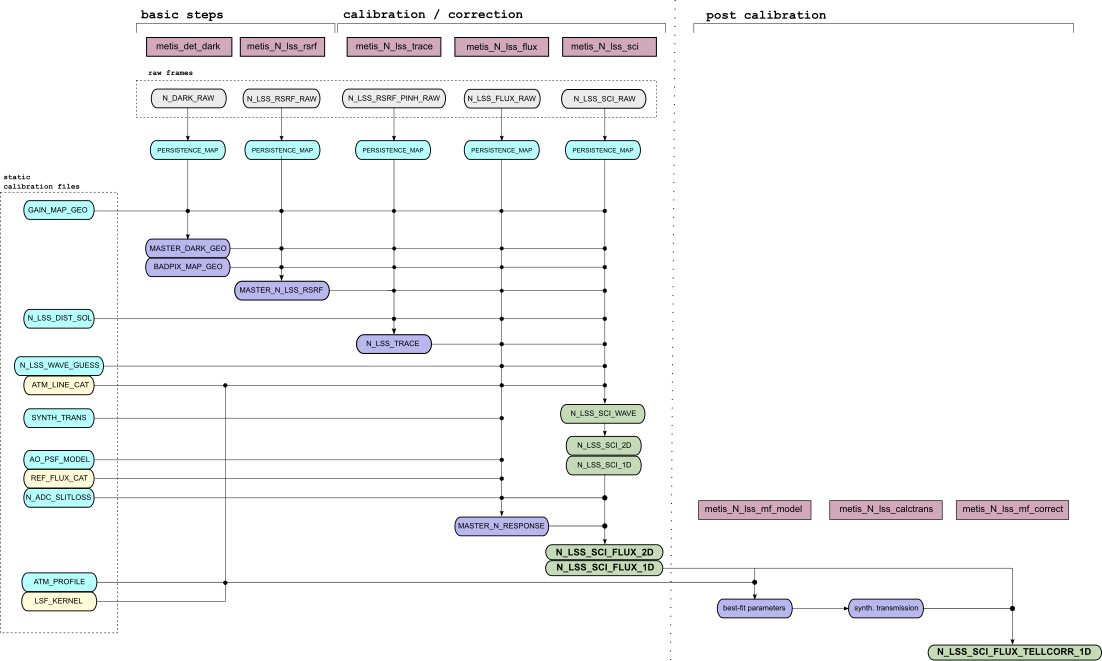
\includegraphics[width=0.9\textheight]{figures/N_LSS_pipeline_wf_draft_latest_v0.74.png}
  \caption[Reduction cascade and association map for N long-slit
  spectroscopy]{Reduction cascade and association map for long-slit
    spectroscopy in the N bands. }
  \label{Fig:NLssAssomap}
\end{sidewaysfigure}

%% ---- Table: N long-slit spectroscopy
\begin{sidewaystable}
  \footnotesize
  \begin{center}
    \caption[Data Processing table for N-band long-slit spectroscopy]{%
      Data Processing table for N long-slit spectroscopy
      calibration mode}\bigskip
    \label{Tab:NLssDatProc}
    \begin{tabular}{|l|l|l|l|l|l|}
      \hline
      Data Type   & Classification & Recipe (Level)	& FITS Keywords & static CalibDB & Products\\
    (Templates) & Keywords	 & Processing steps	&		&	  &	\\
    \hline
    \TPL{DARK}	& \CODE{DPR.CATG==CALIB} & \hyperref[sssec:metis_det_dark]{\REC{metis_det_dark}} & Exposure time	& \hyperref[dataitem:gainmap2rg]{\PROD{GAIN_MAP_GEO}}	& Averaged dark frame\\
    		& \CODE{DPR.TYPE==DARK}  &			&		&	& Bad pixel map\\
    		& \CODE{DPR.TECH==IMAGE}  &			&		&	& \\
    \hline
    \TPL{FLAT}	& \CODE{DPR.CATG==CALIB} & \hyperref[rec:lssnrsrf]{\REC{metis_N_lss_rsrf}} & Exposure time	& \hyperref[dataitem:gainmap2rg]{\PROD{GAIN_MAP_GEO}}	& Averaged, normalized flatfield (\ac{RSRF}\\
    		& \CODE{DPR.TYPE==FLAT}  &			&	Grism	&	& Bad pixel map\\
    		& \CODE{DPR.TECH==SPECTRUM}  &			& Slit		&	& \\
    \hline
         	& \CODE{DPR.CATG==CALIB} & \hyperref[rec:lssntrace]{\REC{metis_N_lss_trace} }& Exposure time	& \hyperref[dataitem:gainmap2rg]{\PROD{GAIN_MAP_GEO}}	& Order location\\
    		& \CODE{DPR.TYPE==FLAT}  &			&	Grism	&	& (polynomial fit)\\
    		& \CODE{DPR.TECH==SPECTRUM}  &			&	Slit	&	& \\
    \hline
    \TPL{FLUX,STD} & \CODE{DPR.CATG==CALIB} & \hyperref[rec:lssnflux]{\REC{metis_N_lss_flux}} & Object name (Flux STD) & \hyperref[dataitem:gainmap2rg]{\PROD{GAIN_MAP_GEO}} & Instrumental\\
    		& \CODE{DPR.TYPE==FLUX,STD}   &			   & Exposure time & \hyperref[dataitem:nlsswaveguess]{\STATCALIB{N_LSS_WAVE_GUESS}} & response function\\
    		& \CODE{DPR.TECH==SPECTRUM}   &			   & Grism		& \hyperref[dataitem:atmlinecat]{\EXTCALIB{ATM_LINE_CAT}}	& \\
    		& \CODE{PRO.CATG==SPECTRUM}   &  &  Slit & \hyperref[dataitem:nsynthtrans]{\STATCALIB{N_SYNTH_TRANS}} & \\
    		& & & & \hyperref[dataitem:nadcslitloss]{\STATCALIB{N_ADC_SLITLOSS}} &\\
    		& & & &  \hyperref[dataitem:reffluxcat]{\STATCALIB{REF_FLUX_CAT}} &\\
    		& & & & \hyperref[dataitem:aopsfmodel]{\EXTCALIB{AO_PSF_MODEL}} &\\
    		& & & & \hyperref[dataitem:nlssdistsol]{\STATCALIB{N_LSS_DIST_SOL}} &\\
    		& & & & \hyperref[dataitem:reffluxcat]{\STATCALIB{REF_FLUX_CAT}} &\\
    \hline
    \TPL{SCIENCE} & \CODE{DPR.CATG==SCIENCE} & \hyperref[rec:lssnsci]{\REC{metis_N_lss_sci}} & Object name & \hyperref[dataitem:gainmap2rg]{\PROD{GAIN_MAP_GEO}}  & Science grade spectrum\\
    		& \CODE{DPR.TYPE==OBJECT}   &			   & Exposure time &  \hyperref[dataitem:atmlinecat]{\EXTCALIB{ATM_LINE_CAT}} &\\
    		& \CODE{DPR.TECH==SPECTRUM}  &			&	Grism	&\hyperref[dataitem:nadcslitloss]{\STATCALIB{N_ADC_SLITLOSS}}	& \\
    		& \CODE{PRO.CATG==SPECTRUM}   &  & Slit & \hyperref[dataitem:nlsswaveguess]{\STATCALIB{N_LSS_WAVE_GUESS}} & \\
    		& & & & \hyperref[dataitem:nlssdistsol]{\STATCALIB{N_LSS_DIST_SOL}} &\\
    \hline
            & \CODE{DPR.CATG==SCIENCE} & \hyperref[rec:NLSSmfmodel]{\REC{metis_N_lss_mf_model}} & Object name & \hyperref[dataitem:lsfkernel]{\STATCALIB{LSF_KERNEL}}	 & Best-fit \\
    		& \CODE{DPR.TYPE==OBJECT}   &			  & & \hyperref[dataitem:atmprofile]{\EXTCALIB{ATM_PROFILE}}  & \texttt{molecfit} parameters\\
    		& \CODE{DPR.TECH==TBD}  &			&		& \hyperref[dataitem:atmlinecat]{\EXTCALIB{ATM_LINE_CAT}}	& \\
    		& \CODE{PRO.CATG==TBD}   &  &  & start parameter set & \\
    \hline
            & \CODE{DPR.CATG==SCIENCE} & \hyperref[rec:NLSSmfcalctrans]{\REC{metis_N_lss_mf_calctrans}} & Object name & \hyperref[dataitem:atmlinecat]{\EXTCALIB{ATM_LINE_CAT}}	 & synthetic \\
    		& \CODE{DPR.TYPE==LSS}   &		&	   &  & Transmission curve\\
    		& \CODE{DPR.TECH==TBD}  &			&		&  	& \\
    		& \CODE{PRO.CATG==TBD}   &  &  & & \\
    \hline
            & \CODE{DPR.CATG==SCIENCE} & \hyperref[rec:NLSSmfcorrect]{\REC{metis_N_lss_mf_correct}} & Object name & 	 & Absorption corrected\\
    		& \CODE{DPR.TYPE==LSS}   &			   &  & synthetic Transmission curve & science spectrum\\
    		& \CODE{DPR.TECH==TBD}  &			&		&	& \\
    		& \CODE{PRO.CATG==TBD}   &  &  & & \\
    \hline
    \end{tabular}
  \end{center}
\end{sidewaystable}

\subsubsection{Static calibration database}\label{lss:static_calib}
The static calibration database comprises several data sets, some are updated from time to time:
\begin{itemize}
    \item \hyperref[dataitem:gainmap2rg]{\hyperref[dataitem:gainmap2rg]{\PROD{GAIN_MAP_2RG}}} and \hyperref[dataitem:gainmapgeo]{\hyperref[dataitem:gainmap2rg]{\PROD{GAIN_MAP_GEO}}}: These are the detector gain maps of the detectors (2RG=Hawaii2RG, LM-band; GEO=Geosnap, N-band), which are created by the recipe \hyperref[sssec:metis_det_lingain]{\REC{metis_det_lingain}} (see Section~\ref{sssec:metis_det_lingain}). This recipe also checks the linearity of the pixels and is carried out every once in a while (yearly, TBD, see \cite{METIS-calibration_plan}) as we assume the detectors to be fairly stable.
    \item \hyperref[dataitem:lasertab]{\STATCALIB{LASER_TAB}}: The \ac{WCU} provides laser sources for the first guess of the wavelength solution. The main laser frequencies are fixed (\cite{METIS-calibration_plan}) and given in a static table.
    \item \hyperref[dataitem:atmlinecat]{\EXTCALIB{ATM_LINE_CAT}}: The main wavelength calibration will be done by means of atmospheric lines, most probably based on the \ac{HITRAN}\footnote{\url{https://hitran.org/}}. They are given in a static catalogue. This database is also required by the telluric correction package \texttt{molecfit}.
    \item \hyperref[dataitem:lmsynthtrans]{\STATCALIB{LM_SYNTH_TRANS}}/\hyperref[dataitem:nsynthtrans]{\STATCALIB{N_SYNTH_TRANS}}: For the determination of the continuum of flux standard stars a rough telluric correction is needed. We intend to apply static transmission curves for that purpose as we deem it to be sufficient and more time efficient than applying the telluric correction package \texttt{molecfit} every time. This static transmission curve will be determined during commissioning via \texttt{molecfit}.
    \item \hyperref[dataitem:aopsfmodel]{\EXTCALIB{AO_PSF_MODEL}}: For the determination of \ac{AO}-induced slit losses we intend to use a static \ac{PSF} model, which is scaled by the \ac{AO} telemetry data. Details on that are TBD.
    \item \hyperref[dataitem:reffluxcat]{\STATCALIB{REF_FLUX_CAT}}: The absolute flux calibration will be done by observations of specific flux standard stars, which are compared to their theoretical models. The \hyperref[dataitem:reffluxcat]{\STATCALIB{REF_FLUX_CAT}} will contain these models. Currently, the catalogue of flux standard stars comprises the stars from the catalogue of the \ac{VISIR} instrument.

    \item \hyperref[dataitem:tssmodelcat]{\STATCALIB{TSS_MODEL_CAT}}: In some cases, the default modelling method for the telluric correction might not be possible or leading to bad results. We therefore foresee the possibility to use telluric standard stars. For the determination of the transmisison function a model of the selected telluric star is required. In this table, a model of a set of such stars
    \item \hyperref[dataitem:tssconttab]{\STATCALIB{TSS_CONT_TAB}}: 

    \item \hyperref[dataitem:lmadcslitloss]{\STATCALIB{LM_ADC_SLITLOSS}}/\hyperref[dataitem:nadcslitloss]{\STATCALIB{N_ADC_SLITLOSS}}: It is expected that the fixed positions of the \ac{ADC} will introduce specific slit losses. These losses are determined in the recipes \hyperref[rec:metislmadcmslitloss]{\REC{metis_lm_adc_slitloss}} and \hyperref[rec:metisnadcmslitloss]{\REC{metis_n_adc_slitloss}} (see Section~\ref{sssec:adc_slitlosses} and \cite{METIS-calibration_plan}). As these losses are assumed to be very stable, these recipes will be carried out only rarely.
    \item \hyperref[dataitem:atmprofile]{\EXTCALIB{ATM_PROFILE}} and \hyperref[dataitem:lsfkernel]{\STATCALIB{LSF_KERNEL}}: The telluric correction package \texttt{molecfit} requires an atmospheric profile incorporating height information of the temperature, pressure and molecular abundances as input. Currently we use a static profile (equatorial \texttt{equ.atm}\footnote{\url{https://eodg.atm.ox.ac.uk/RFM/atm/}}) as starting point of the fit of the molecular column densities. In addition, a kernel for the \ac{LSF} is provided. We intend to determine the kernel during commissioning and use this as input. However, it is still unclear in how far the \ac{AO} influences that kernel. The current baseline is to use the static \hyperref[dataitem:lsfkernel]{\STATCALIB{LSF_KERNEL}} as starting point for fitting the line spread function.
    \item \hyperref[dataitem:nlssdistsol]{\STATCALIB{N_LSS_DIST_SOL}}/\hyperref[dataitem:nlsswaveguess]{\STATCALIB{N_LSS_WAVE_GUESS}}: First guess solutions of the N-band LSS mode are static due to the absence of laser sources after \ac{AIT}. As the instrument is expected to be very stable, these calibration files will be created only once and kept static.
\end{itemize}  % TO BE EDITED BY INNSBRUCK ONLY!!!!!

\clearpage
% IFU-mode
% \input{05_3-Overview_IFU}

\clearpage
\clearpage

\section{Algorithms / Mathematical description}
\label{sec:algorithms}
\input
\subsection{High-contrast imaging with the apodizing phase plate}
\label{ssec:algo_app_imaging}

LM-band imaging data taken with the apodizing phase plate undergo the
same basic reduction as standard imaging data. \TODO{Does this include
  background subtraction or is the background subtracted during the
  ADI processing?}



\begin{enumerate}
\item Locate the positions of the PSFs with respect to each other
  (dither correction).
\item Center the leakage PSF in the frames.
\item Extract the coronagraphic PSFs and combine them into a single
  cube (see Fig.~\ref{fig:app_psf_combine}). This has almost
  360\degr\ dark zones.
\item Median combine the cube to obtain the reference PSF image.
\item Subtract PSF image from all layers of the cube.
\item Derotate all layers to correct for field rotation, taking into
  account a static mask to reject noisy border regions of the dark
  zones.
\item Sum the layers to obtain final image.
\end{enumerate}

\begin{figure}
  \centering
  \resizebox{0.8\textwidth}{!}{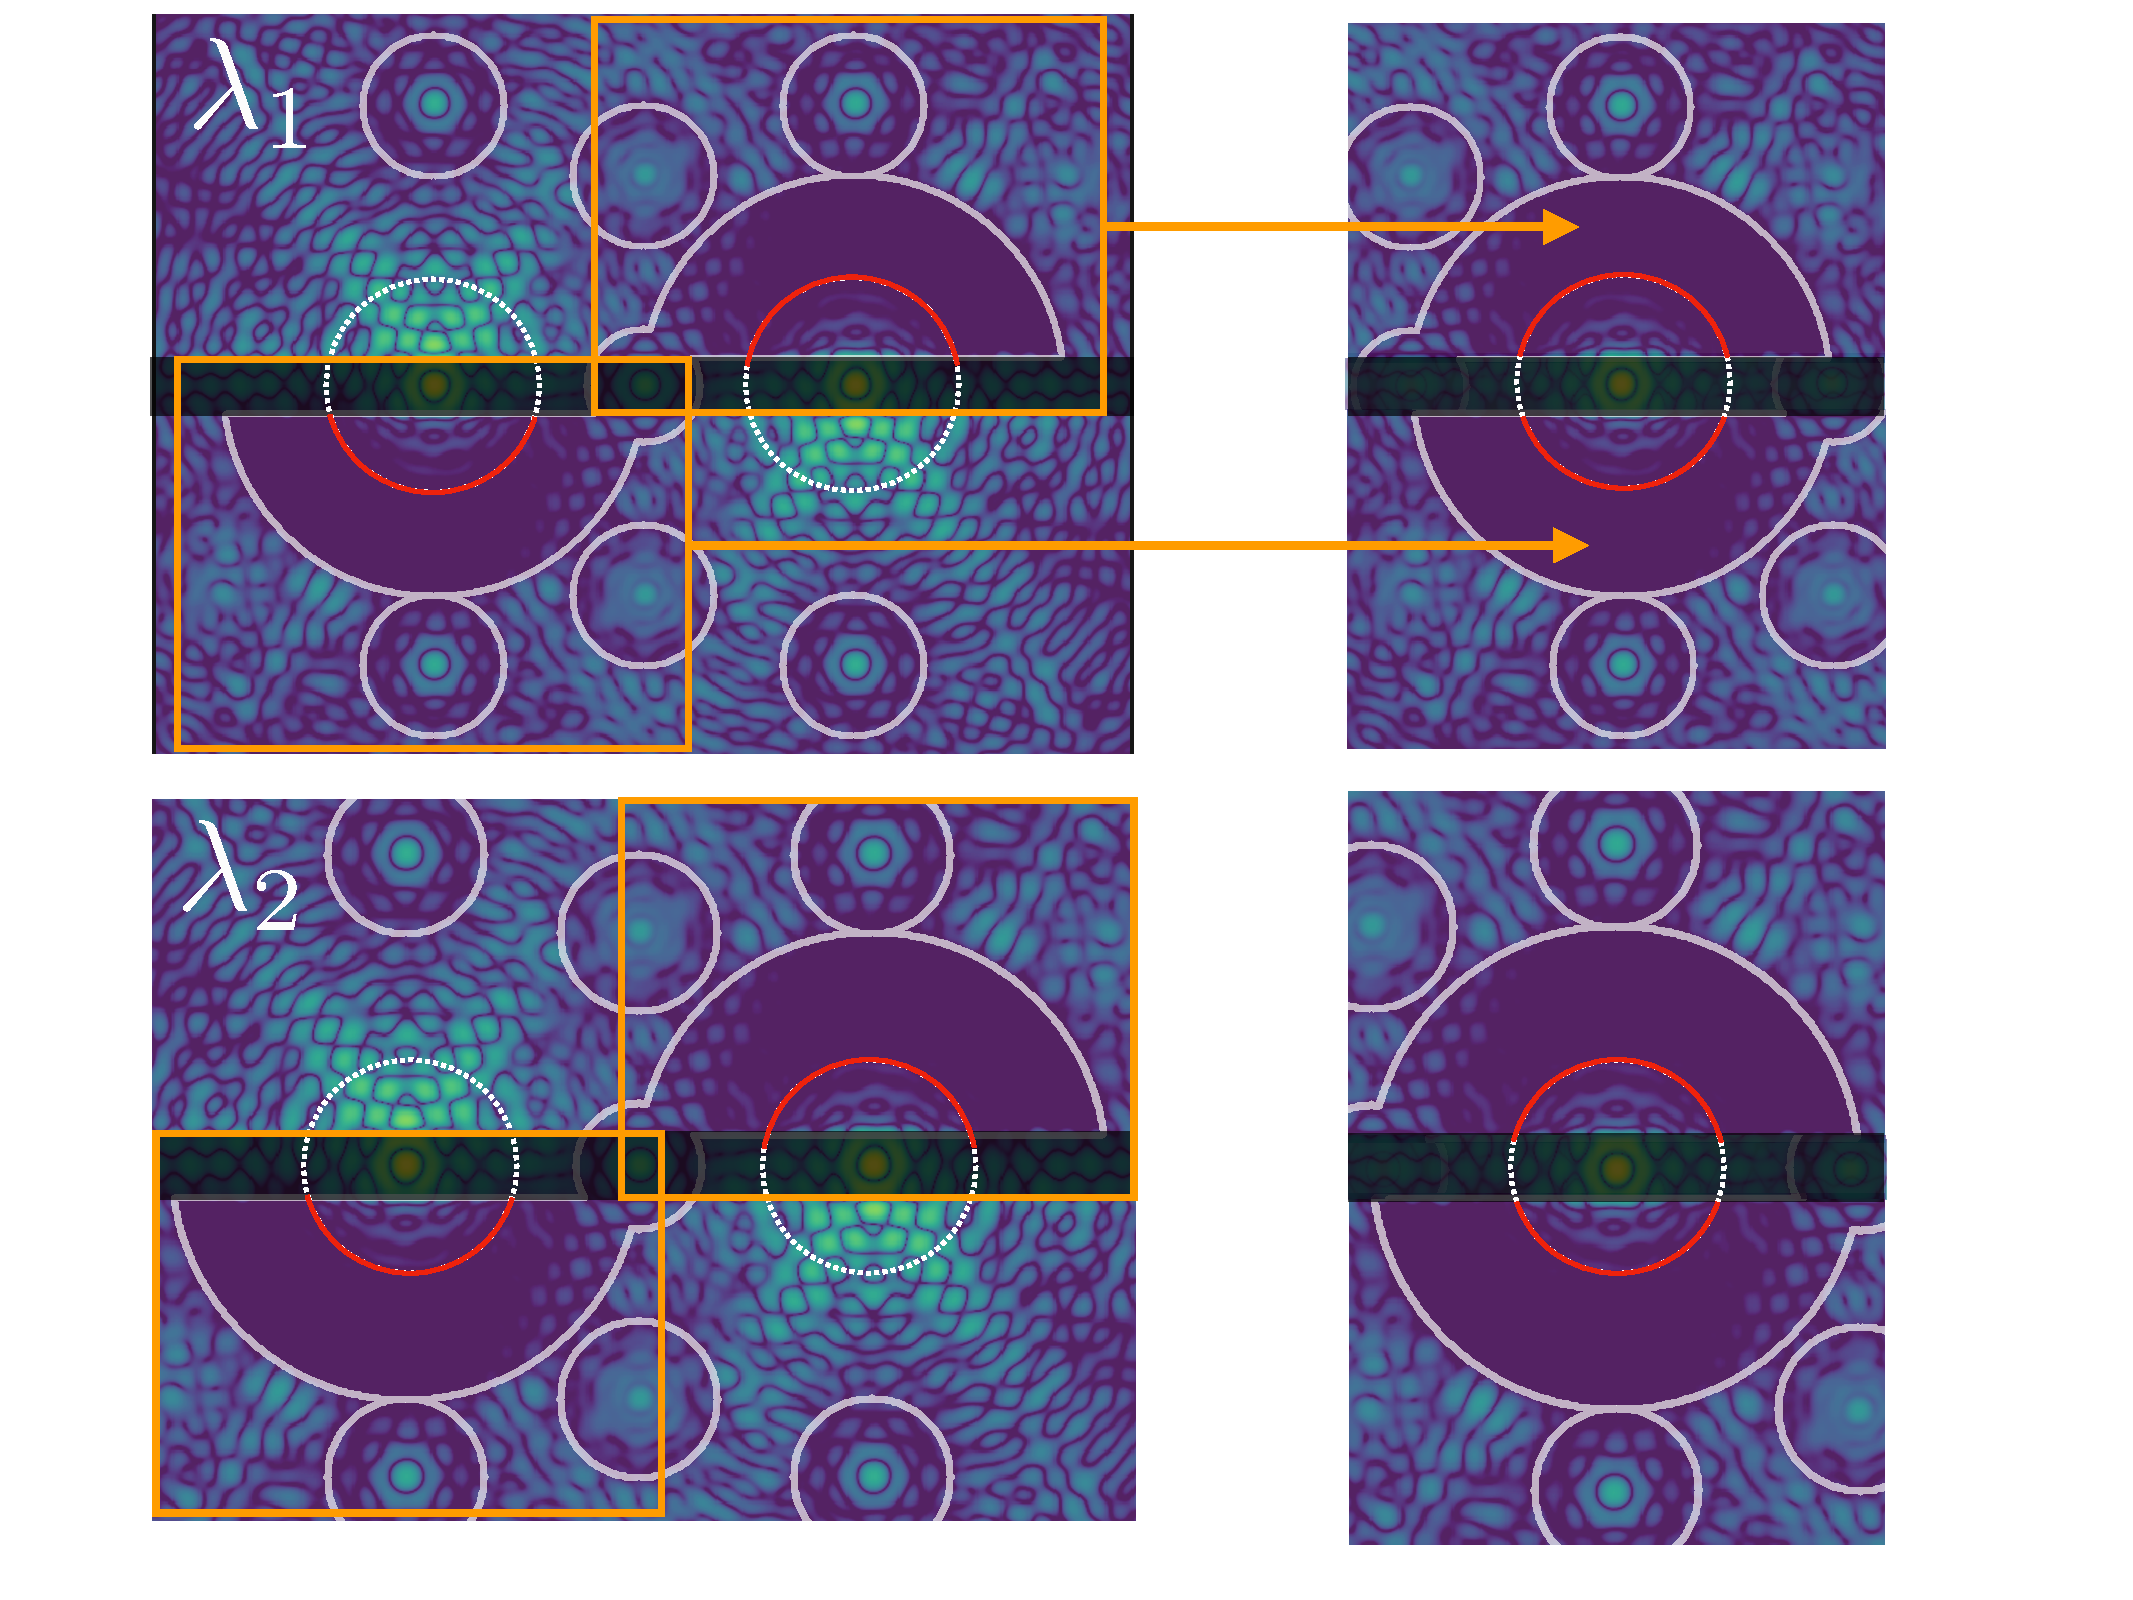
\includegraphics{vAPP_data_reduction}}
  \caption{Combination of the coronagraphic PSFs of APP observations
    into a single PSF with 360\degr\ dark zones. \TODO{This is a figure
      by David Doelman. The layout of the PSFs is not what we expect
      for METIS, therefore needs to be updated.}}
  \label{fig:app_psf_combine}
\end{figure}

%%% Local Variables:
%%% TeX-master: "METIS_DRLD"
%%% End:

\subsection{Long-slit spectroscopy mode}
\label{ssec:algo_lss_spectroscopy}

%-----------------------------------------------------------------------------------------
\subsubsection{Order background contamination removal}\label{ssec:orderbg}
Order background contamination may arise from internal straylight probably covering larger areas of the detector. Since it is expected to be low frequency only, its removal can be achieved by a low-order 2D polynomial fit 
\begin{equation}
    z = (a_0 + a_1x + a_2y + a_3x^2 + a_4x^2y + a_5x^2y^2 + a_6y^2 + a_7xy^2 + a_8xy ...)
\end{equation}
and a subsequent subtraction. The fitting points/regions must be chosen to be outside the \ac{LSS} order. Whereas these fitting points/regions can be chosen on fairly regular basis due to the straight order geometry in the \ac{LSS} mode, the degree of the polynomial depends on the actual straylight. This can be determined only during the testing phase when first real data are available.

%-----------------------------------------------------------------------------------------
\subsubsection{Order detection and rectification}\label{ssec:orderhandling}
The algorithms for order detection and rectification are adopted from \cite{pis02,pis21}.
In brief, the selection of pixels that may belong to spectral \ac{LSS} order is done by first smoothing each column and then selecting pixels above the median of the difference between the original
and the smoothed column, i.e. pixel $(x,y)$ is selected if
\begin{equation}
    I(x,y) > \bar{I}(x,y) + \mathrm{Median} ( I(x,y) - \bar{I}(x,y) ) .
\end{equation}
In the following a clustering analysis is performed, which associates connected groups of pixels. This is done scanning rows and columns and identifying neighbouring pixels selected in the previous step as belonging to the same cluster if $\delta x$ and $\delta y$ differ by at most 1. As spectral orders may be partitioned into different clusters because of e.g. detector defects, polynomial fits to the clusters are performed and the pairwise extensions of the fits to consecutive clusters are compared to identify which clusters are to be merged according to predefined criteria for the goodness of match. For each order, the detection algorithm yields a polynomial description of order location on the detector (the order center and its edges), an uncertainty estimate
for the fitted polynomial, and the first and last columns to be used during spectrum extraction. 
%The upper and lower edges of the orders are also traced and fitted by the order tracing algorithm using the pinhole frames with the flatfield lamp. 
Order rectification is achieved using the PyReduce algorithm described by \cite{pis21} that can account for both tilt and curvature of the slit image.   

%-----------------------------------------------------------------------------------------
\subsubsection{Spectroscopic flux calibration strategy}\label{ssec:fluxcal}
Flux calibration implies the conversion of ADUs to physical units. This is done by comparing the observed spectrum of a standard star with its reference spectrum as seen without atmospheric and instrument/telescope signatures, facilitating the response function to be determined. The response function describes the optical throughput of the optical system, i.e. the instrumental effect on the flux. In principle this is a standard procedure and in \ac{METIS} basically the same approach as described in the \ac{HDRL} will be closely followed.

\textcolor{red}{TBD: slit flux losses due to PSF (cf. MICADO)?????}


%-----------------------------------------------------------------------------------------
\subsubsection{Telluric absorption correction}\label{ssec:tellcorr}
Due to the dense molecular absorption arising from the Earth's atmosphere, nearly every \c{MIR} regime spectrum requires a correction for these telluric features. The required atmospheric transmission curve can be achieved either by specific observations of a telluric standard star (\ac{TSS}, the "classical" way) or by a modelling approach. \\
\paragraph{Classic \ac{TSS} approach:\newline}
A telluric standard star (\ac{TSS}) spectrum is taken ideally directly before/after the science observations near the science target position (or at least at the same airmass) to probe the same pathway through the Earth's atmosphere. This \ac{TSS}-spectrum is processed in the same way as the science spectrum (except the absolute flux calibration). To remove intrinsic stellar features this spectrum is corrected with a model spectrum of this \ac{TSS}. Finally its continuum is normalised to unity. The resulting normalised spectrum (ideally) only contains the fingerprint of the Earth's atmospheric absorptions and can be used for the telluric correction.\\
There are several sources for model spectra available:
\begin{itemize}
    \item Cohen set (\cite{coh99}): Set of 422 stellar model templates, mainly K and M giants. One of the standard sets in \ac{MIR}.
    \item The SPEX \ac{IRTF} Spectral library\footnote{\url{http://irtfweb.ifa.hawaii.edu/~spex/IRTF_Spectral_Library/}}: Set of observed stellar spectra (F to M-type, some carbon and S-type stars and L and T dwarfs) in the range $0.8...5.0\mu$m mostly at a resolving power of $R\equiv\lambda/\Delta\lambda\sim2,000$.
    \item Phoenix library\footnote{\url{https://phoenix.astro.physik.uni-goettingen.de/}}\cite{phoenix}: Library of synthetic medium and high resolution spectra between $0.5...5.5\mu$m covering a wide stellar parameter space ($2,300\textrm{K}\leq T_\textrm{eff}\leq12,000\textrm{K}$; $0.0\leq\log g\leq+6.0$; $-4.0\leq$[Fe/H]$\leq+1.0$; $0.2\leq$[$\alpha$/Fe]$\leq+1.2$). \\
\end{itemize}
The \ac{METIS} consortium will look into that topic and to assemble a set of appropriate \ac{TSS} stars.

\paragraph{Modelling synthetic transmission spectra:\newline} In the last years the modelling method has evolved. It is based on radiative transfer modelling of the Earth's atmosphere (\cite{mf1, mf2, molecfit}\footnote{\url{https://www.eso.org/sci/software/pipelines/skytools/molecfit}}). A height model of the Earth's atmosphere containing information of pressure, temperature and the concentration of molecules in combination with a radiative transfer model and a molecular line list is used to determine the transmission of the Earth's atmosphere at the time of observations. The approach by fitting specific molecular absorption features in the science spectra. The best-fit transmission function is finally used for the telluric correction.\\
In the past years the approach of modelling transmission curves of Earth's atmosphere has made significant progress leading to versatile and mature software packages for the telluric correction. One of these packages is \texttt{molecfit}\footnote{\url{http://www.eso.org/sci/software/pipelines/skytools/molecfit}} (\cite{mf1, mf2}). This package is optimised for the ESO framework and ESO instruments and is also foreseen to be used for \ac{METIS}.\\
The outcome of the \ac{ELT} working group meeting of 2021-03-15 was that future instrument pipelines should include dedicated recipes based on the telluric correction \texttt{telluriccorr} library \cite{telluriccorr}. This package is based on \texttt{molecfit} and will be provided and maintained by \ac{ESO}. The telluric correction will be performed in three dedicated recipes as post-correction   and closely follow the approach as implemented in the \ac{KMOS} pipeline. The three steps comprise the fit of the telluirc features (e.g. \REC{metis_LM_lss_mf_model} for the LM range), the calculation of the transmission curve (e.g. \REC{metis_LM_lss_mf_calctrans}) and the application of the actual correction (e.g. \REC{metis_LM_lss_mf_correct}). For the determination of the \ac{LSF} we primarily rely on the possibilities as offered by the \texttt{telluricorr}/\texttt{molecfit} package, which is based on a fitting of the \ac{LSF} by a combination of a boxcar, Gaussian or Lorentzian. On basis of the commissioning data we will establish a parameter set providing a good starting point for the fits.\\
We also intend to enable the user to include a dedicated line kernel instead, in case a reliable kernel model can be determined with other (external) tools (e.g. a model-based convolution of an internal \ac{LSF}, the slit-widths and/or an \ac{AO} component). In addition, also external supplementary meteorological data (e.g. provided by an \ac{LHATPRO} radiometer) can be included if the \texttt{telluricorr}/\texttt{molecfit} package offers that possibility.

\paragraph{Approach for \ac{METIS}:\newline} 
The modelling approach has become the standard way for the telluric correction in several ESO pipelines as it avoids to spend valuable observing time on taking \ac{TSS} spectra. Since the synthetic transmission function is also noise-free, it also conserves the \ac{SNR} of the science spectrum. It is therefore also foreseen as default method for the \ac{METIS} pipeline.\\
Nevertheless, there might be situations where the classical way becomes the better option. For example, in case the science object's continuum is too weak to be used for fitting telluric features. In addition, \texttt{molecfit} relies on a number of fitting parameters, which might not lead to the best minimum. In particular, the quality of the fit is very sensitive to the incorporated \ac{LSF}-Kernel, whereas the \ac{LSF} of a \ac{TSS} spectrum is naturally (almost) identical.\\
We therefore will include three different approaches for the telluric correction in the \ac{METIS} pipeline (cf. Fig.~\ref{Fig:tellcorrmethods}):
\begin{itemize}
    \item "\textit{molecfit-on-science}": This is the usual way of using \texttt{molecfit}, i.e. the science spectrum ("\texttt{1D SCIENCE SPECTRUM}") is used to determine the state of the Earth's atmosphere and to calculate a synthetic transmission (left branch in Fig.~\ref{Fig:tellcorrmethods})
    \item "classical approach: 
\end{itemize}

\begin{figure}[ht]
  \centering
  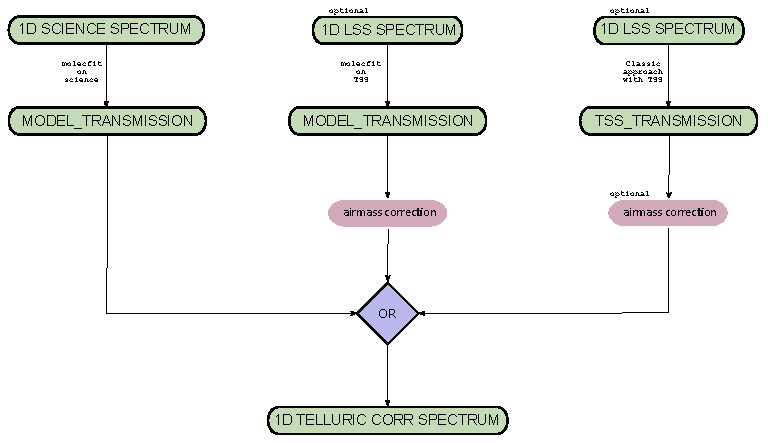
\includegraphics[width=0.9\textwidth]{figures/tell_corr_methods.pdf}
  \caption{Methods for the telluric correction to be included in the \ac{METIS} pipeline.}
  \label{Fig:tellcorrmethods}
\end{figure}


%-----------------------------------------------------------------------------------------
\subsubsection{Object extraction and faint object spectroscopy}\label{sec:fospectro}
The object spectra will be extracted using the optimal extraction described by \cite{pis21} in order to maximized the \ac{SNR}. 
Faint objects will lead to additional requirements for the observation and the data reduction. For the target acquisition a blind offset from a reference source might become necessary in case the actual object cannot be detected directly. For the data reduction, manual interaction with the user is expected to be necessary to define the target position along the slit since automatic object detection algorithms (e.g. optimal extraction %\cite{hor86}) 
rely on a certain \ac{SNR}. This will be implemented as interactive actor in Reflex (or ESO-DPS).
\subsection{Miscellanea}
\label{ssec:miscellanea}

\subsubsection{Parallactic angle}
\label{sssec:parallactic_angle}

The parallactic angle is the angle between the meridian (direction to the celestial north pole) and the hour circle (direction to the zenith) through the target at the time of an observation. Given hour angle $h$ and declination $\delta$ of the target, as well as the latitude $\phi$ of the observatory, the parallactic angle $\eta$ is given by
\begin{equation}
  \label{eq:parallactic_angle}
  \tan\eta = \frac{\cos\phi\sin h}{\sin\phi \cos\delta - \cos\phi \sin\delta \cos h}
\end{equation}
The hour angle is computed from the telescope's pointing altitude and azimuth, or from the target's right ascension and the sidereal time stamp of the exposure.

\subsubsection{Gain, non-linearity}
\label{sssec:gain}

The variance $N_{c}^{2}$ is related to the signal $S_{c}$ via \cite[Section 9.1]{McLean2008}:
\begin{equation}
  \label{eq:signal-variance}
  N_{c}^{2} = \frac{1}{g} S_{c} + R_{c}^{2},
\end{equation}
where $g$ is the gain and $R_{c}$ the readout noise. All quantities with subscript $c$ are in counts (ADU).

\subsubsection{Conversion of wavelengths between vacuum and air regime}\label{ssec:vacair}
For the conversion of $\lambda_\textrm{vac}$ to $\lambda_\textrm{air}$ the \ac{IAU} standard formula provided by Donald Morton \cite{mor00} $\lambda_\textrm{air}=\lambda_\textrm{vac}/n$ is used, where

\begin{eqnarray}\label{eq:air2vac}
\left.\begin{aligned}
    s &=10^4 / \lambda_{\textrm{vac}}\\
    n &= 1+0.0000834254 + \frac{0.02406147}{(130 - s^2)} + \frac{0.00015998}{(38.9 - s^2)}
\end{aligned}\right.
\end{eqnarray}

The reverse transform $\lambda_\textrm{air}$ to $\lambda_\textrm{vac}$ was derived by N. Piskunov\footnote{\url{https://www.astro.uu.se/valdwiki/Air-to-vacuum\%20conversion}}, being $\lambda_\textrm{vac}=\lambda_\textrm{air}*n$ with 

\begin{eqnarray}\label{eq:vac2air}
\left.\begin{aligned}
    s&=10^4 / \lambda_{\textrm{air}}\\
    n&=1 + 0.000083366242 + \frac{0.0240892687}{(130.106592452 - s^2)} + \frac{0.00015997409}{(38.925687933 - s^2)}
\end{aligned}\right.
\end{eqnarray}

All wavelengths in the \ac{LSS} spectroscopic pipeline are given in the vacuum regime. \textcolor{red}{TBD: Also in IFU?}

\subsubsection{Centroid fit}
\label{sssec:centroid}
TBWritten

\subsubsection{Line shape fit}
\label{sssec:linefit}
TBWritten about Gaussian line fitting


%%% Local Variables:
%%% TeX-master: "METIS_DRLD"
%%% End:


%%% Local Variables:
%%% TeX-master: "METIS_DRLD"
%%% End:



\clearpage

\section{Pipeline Recipes / CPL Plugins}
\label{sec:pipeline_recipes}

Throughout this document we use the following color scheme for the
recipe workflows:
\begin{center}
  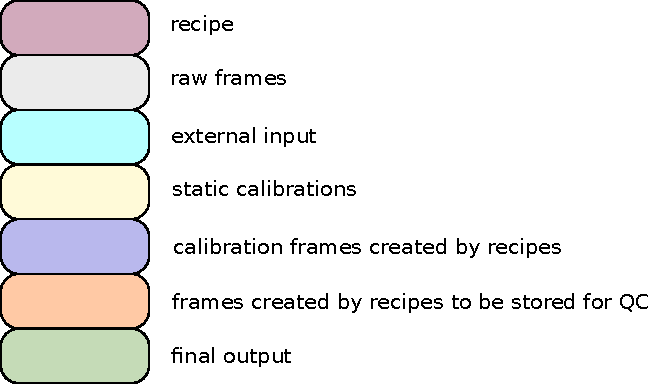
\includegraphics[width=0.3\textheight]{colour_legend}
\end{center}

%% Recipes_Detector.tex
%% Created:     Tue Apr  4 16:37:17 2017 by Koehler@I-Mac
%% Last change: 2020-09-04
%%
%% subsection for Detector Recipes
%%
%%%%%%%%%%%%%%%%%%%%%%%%%%%%%%%%%%%%%%%%%%%%%%%%%%%%%%%%%%%%%%%%%%%%%%%%%%%%%
\subsection{Detector calibration recipes}
\label{Sec:detector_calibration}

METIS will have three focal plane detector arrays:
\begin{itemize}
\item One $2\mathrm{k}\times 2\mathrm{k}$ HAWAII2RG detector used for
  LM-band imaging and slit spectroscopy.
\item One $2\mathrm{k}\times 2\mathrm{k}$ GeoSnap (Teledyne) detector
  used for N-band imaging and slit spectroscopy.
\item An array of four $2\mathrm{k}\times 2\mathrm{k}$ HAWAII2RG
  detectors used for LM-band integral-field spectroscopy.
\end{itemize}
This section lists recipes that calibrate detector characteristics
independent of a specific instrument mode. Where \FITS{_det} appears
in FITS keywords of input or product files, it is taken to mean
\FITS{_LM}, \FITS{_N} or \FITS{_IFU} according to the detector
array for which data are being processed.

\subsubsection{Detector linearity and gain determination recipe \REC{metis_det_lingain}}
\label{sssec:metis_det_lingain}
\label{rec:metis_det_lingain}
\label{rec:metisdetlingain}

The recipe \REC{metis_det_lingain} determines detector (non-)linearity and absolute detector
gain from a set of flat-field frames taken with the broad-band lamp
over a range of detector exposure times (DITs) and flux levels. The
recipe structure will be similar as for \CODE{detmon_ir_lg} % Not a \REC because it is not our recipe
\cite{detmon-manual}; however, further insight into detector behaviour
(in particular of GeoSnap) may necessitate development of more complex
procedures.

The linearity curve is given by the measured background level as a
function of exposure time for constant illumination. For each pixel
the coefficients of a polynomial fit (order TBD) will be recorded in a
coefficient cube, which can in turn be used to correct for
non-linearity in other recipes. Pixels whose coefficients differ
significantly from the majority of pixels will be marked as bad.

Detector gain is typically computed pixelwise as the slope of a linear
fit of the variance against the mean (or median) values over a set of
frames taken over a range of DITs and illumination levels.  For
mid-infrared detectors that suffer from \ac{ELFN}, e.g.\ the AQUARIUS
detector, this approach does not work.  The GeoSnap is not expected to
show \ac{ELFN}, hence gain determination is probably possible.

The set of calibration frames used for this recipes will include
exposures with WCU window closed (\CODE{LAMP OFF}), which will be used
as `dark' frames that captur thermal emission within the
instrument. This is subtracted from all other exposures in the
sequence.

This satisfies \REQ{METIS-5997}.

\newpage
\begin{recipedef}
  Name:                & \hyperref[rec:metis_det_lingain]{\REC{metis_det_lingain}}                                                             \\
  Purpose:             & determine non-linearity and gain of the detectors                                   \\
  Requirements:        & \REQ{METIS-5997}                                                                    \\
  Type:                & Calibration                                                                         \\
  Templates:           & \TPL{METIS_img_lm_cal_DetLin}                                                       \\
                       & \TPL{METIS_img_n_cal_DetLin}                                                        \\
                       & \TPL{METIS_ifu_cal_DetLin}                                                          \\
  Input data:          & \hyperref[dataitem:detlin_det_raw]{\RAW{DETLIN_det_RAW}}: (set of \FITS{FLAT,LAMP} frames taken with increasing DIT) \\
                       & \hyperref[dataitem:dark_internal_det_raw]{\RAW{DARK_INTERNAL_det_RAW}}: (set of internal darks taken at the start of the template) \\
  Matched keywords:    & Subsystem ID \TODO{TBD}                                                             \\
  Algorithm:           & Subtract instrument dark (\CODE{hdrl_imagelist_sub_image}).                         \\
                       & Compute mean and variance for each frame (\CODE{TBD}).                              \\
                       & Gain is determined as the slope of variance against mean (\hyperref[drl:metis_derive_gain]{\CODE{metis_derive_gain}}) \\
                       & Fit polynomial of value as a function of DIT and illumination level for each pixel (\hyperref[drl:metis_derive_nonlinearity]{\CODE{metis_derive_nonlinearity}}). \\
                       & Flag pixels with coefficients significantly different from the mean of all pixels. (\CODE{hdrl_bpm_fit_compute}) \\
  Output data:         & \hyperref[dataitem:gain_map_det]{\PROD{GAIN_MAP_det}}                                    \\
                       & \hyperref[dataitem:linearity_det]{\PROD{LINEARITY_det}}                                 \\
                       & \hyperref[dataitem:badpix_map_det]{\PROD{BADPIX_MAP_det}}                                \\
  Expected accuracies: & \TODO{TBD}                                                                          \\
  QC1 parameters:      & \hyperref[qc:qc_lin_gain_mean]{\QC{QC LIN GAIN MEAN}}                                    \\
                       & \hyperref[qc:qc_lin_gain_rms]{\QC{QC LIN GAIN RMS}}                                      \\
                       & \hyperref[qc:qc_lin_num_badpix]{\QC{QC LIN NUM BADPIX}}                                  \\
  hdrl functions:      & \CODE{hdrl_imagelist_sub_image}                                                     \\
                       & \CODE{hdrl_bpm_fit_compute}                                                         \\
\end{recipedef}

\begin{figure}[hb]
  \centering
  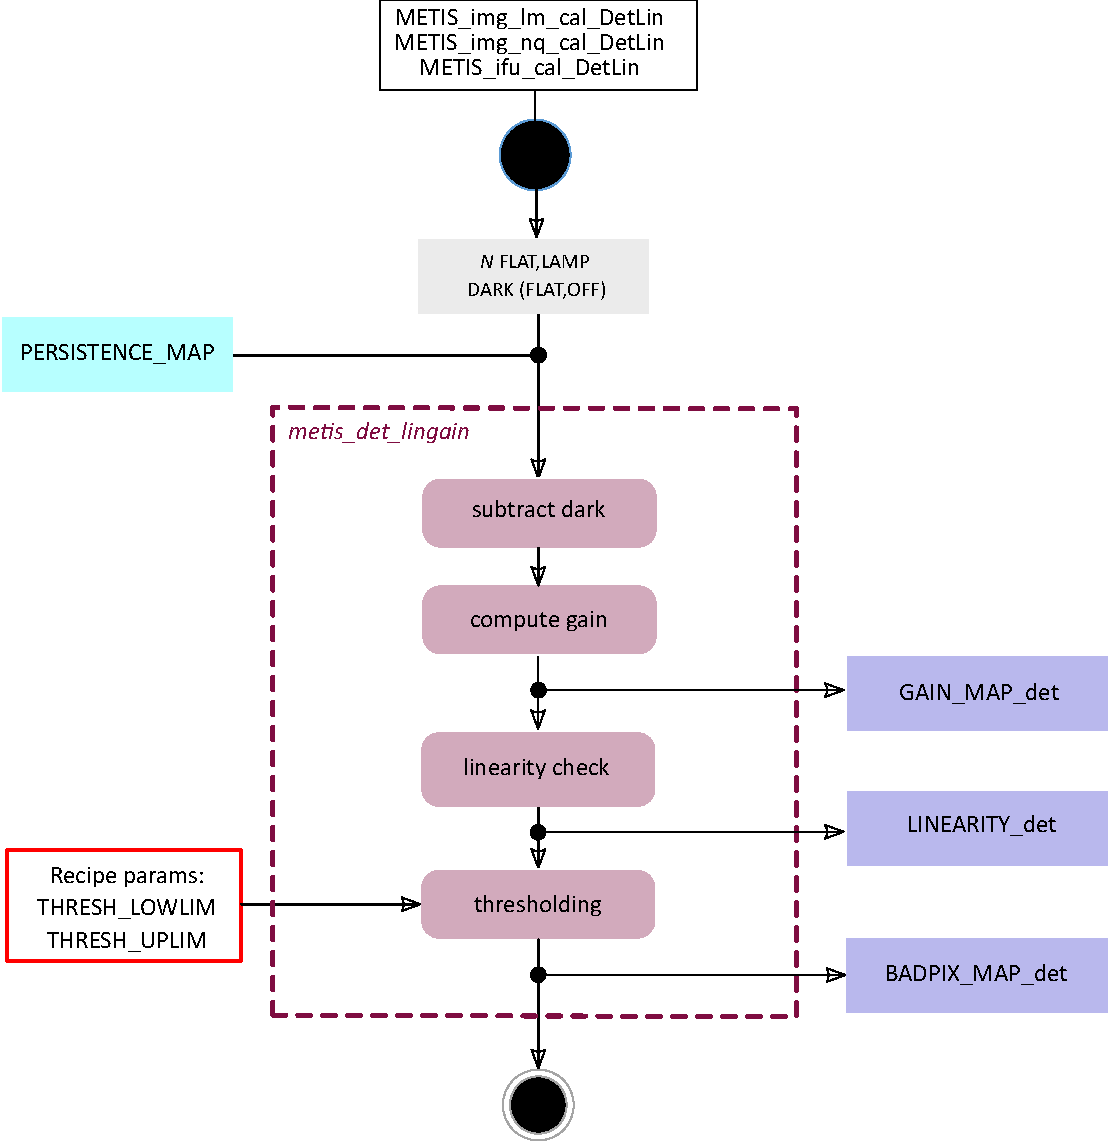
\includegraphics[width=0.65\textwidth]{metis_det_lingain}
  \caption[Recipe: \REC{metis_det_lingain}]{\REC{metis_det_lingain} --
    determination of linearity and gain of the detectors.}
  \label{Fig:rec_det_lingain}
\end{figure}


\clearpage

\subsubsection{Master dark recipe \REC{metis_det_dark}}
\label{sssec:metis_det_dark}
\label{rec:det_dark}
\label{rec:metis_det_dark}

Darks are taken in daytime for all science detectors
\cite{METIS-calibration_plan}. The data will be classified by detector
(e.g.~\FITS{DET.ID} and \FITS{DET.CHIP.ID}) and integration time
(\FITS{DET.DIT}).\footnote{The dark current is not expected to depend on the readout mode of the detectors. Should hardware tests reveal such a dependence, the recipe will be amended to classify on readout mode as well.} There will be ``METIS-dark''
(with the CLOSED position of the CFO-PP1 wheel) and ``Imager-dark''
(with the CLOSED position in the subsystem PP1), to be distinguished
by keyword \TBD. The former will be used for pipeline processing, the
latter for monitoring purposes.

Each set of raw dark frames is processed into a master dark. For the
IFU, both raw frames and master dark have four extensions
corresponding to the four detectors in the focal-plane array. The
recipe also produces bad pixel masks by identifying hot pixels whose
dark current differs significantly (by more than $\pm 5\sigma$) from
the average over the detector.

This fulfills \REQ{METIS-6063}.

\begin{recipedef}
  Name:                & \hyperref[rec:metis_det_dark]{\REC{metis_det_dark}}                                                        \\
  Purpose:             & determine the dark current of the detectors                                 \\
  Requirements:        & \REQ{METIS-6063}                                                            \\
  Type:                & Calibration                                                                 \\
  Templates:           & \TPL{METIS_gen_cal_dark}                                                    \\
  Input data:          & \hyperref[dataitem:linearity_det]{\STATCALIB{LINEARITY_det}}  \\
                       & \hyperref[dataitem:persistence_map]{\EXTCALIB{PERSISTENCE_MAP}}  \\
                       & \hyperref[dataitem:dark_det_raw]{\EXTCALIB{DARK_det_RAW}}  \\
  Parameters:          & Combination method (\texttt{median}, \texttt{mean},
                         \texttt{sigclip},\dots)                                                  \\
                       & Parameters for combination methods                                          \\
                       & Thresholds for deviant-pixel identification                                      \\
  Algorithm:           & Group files by detector and \texttt{DIT}, based on header keywords           \\
                       & Call function \DRL{metis_determine_dark} for each set of files\\
                       & Compute median or average of input frames to improve statistics.            \\  % separate routine, or part of determine dark
                       & call \DRL{metis_update_dark_mask} to flag deviant pixels \\
  Output data:         & \hyperref[dataitem:master_dark_det]{\PROD{MASTER_DARK_det}}                                                      \\
% The BPM_COLD_det and BPM_HOT_det do not seem to add value that BADPIX_MAP_det
% does not already provide. Furthermore, the COLD/HOT specific items are not
% otherwise used in the design, so it seems simpler to just remove them.
%                       & \hyperref[dataitem:bpm_cold_det]{\PROD{BPM_COLD_det}}                                                         \\
%                       & \hyperref[dataitem:bpm_hot_det]{\PROD{BPM_HOT_det}}                                                          \\
                       & \hyperref[dataitem:badpix_map_det]{\PROD{BADPIX_MAP_det}}                                                          \\
  Expected accuracies: & \TBD                                                                         \\
  QC1 parameters:      & \QC{QC DARK MEAN}                                                              \\
                       & \QC{QC DARK MEDIAN}                                                            \\
                       & \QC{QC DARK RMS}                                                               \\
                       & \QC{QC DARK NBADPIX}                                                             \\
                       & \QC{QC DARK NCOLDPIX}                                                               \\
                       & \QC{QC DARK NHOTPIX}                                                                \\
                       & (more \TBD)                                                                  \\
  hdrl functions:      & \CODE{hdrl_bpm_3d_compute}                                 \\
                       & \CODE{hdrl_imagelist_collapse}                             \\
\end{recipedef}

\begin{figure}[hb]
  \centering
  \includegraphics[width=0.5\textwidth]{figures/metis_det_dark_v0.83.pdf}  % RemarK. The original file: figures/metis_det_dark.pdf is still available
  \caption[Recipe: \REC{metis_det_dark}]{\REC{metis_det_dark} -- creation of master
    dark and bad pixel maps}
  \label{Fig:rec_det_dark}
\end{figure}

\clearpage

\subsubsection{Persistence map creation recipe \REC{metis_det_persistence}}
\label{sssec:metis_det_persistence}

Infrared detectors show persistent signal due to charges trapped on a
variety of timescales. The correction for a given science or
calibration exposure is built from a sequence of exposures preceding
the exposure in question. As these may include exposures taken for
another proprietary programme, the recipe is run by ESO on data taken
from the science archive and its products are again ingested into the
archive.

\begin{recipedef}\label{rec:metis_det_persistence}
  Name:                & \hyperref[rec:metis_det_persistence]{\REC{metis_det_persistence}}           \\
  Purpose:             & compute persistence correction maps        \\
  Requirements:        & \REQ{METIS-9145}                      \\
  Type:                & Calibration                           \\
  Templates:           & --                                    \\
  Parameters:          & \TBD                                  \\
  Algorithm:           & see hdrl functions:                   \\
  Output data:         & \hyperref[dataitem:persistence_map]{\PROD{PERSISTENCE_MAP}}                \\
  Expected accuracies: & \TBD                                  \\
  QC1 parameters:      & see hdrl functions:                   \\
  hdrl functions:      & \TBD (\CODE{hdrl_persistence_compute} \\
\end{recipedef}

\begin{figure}[hb]
  \centering
  \resizebox{0.6\textwidth}{0.1\textwidth}{\TODO{\fbox{Figure to be done}}}
  \caption[Recipe:
  \REC{metis_det_persistence}]{\REC{metis_det_persistence} -- creation
    of persistence correction frames.}
  \label{Fig:rec_det_persistence}
\end{figure}

%%%%%%%%%%%%%%%%%%%%%%%%%%%%%%%%%%%%%%%%%%%%%%%%%%%%%%%



%%% Local Variables:
%%% TeX-master: "METIS_DRLD"
%%% End:


\subsection{LM-band imaging}
\label{ssec:recipes_img_lm}

\subsubsection{LM-band imaging flatfield}
\label{lm_img_flatfield}
\label{rec:lm_img_flatfield}
\label{sssec:lm_img_flatfield}
\label{metis_lm_img_flat}
\label{rec:metis_lm_img_flat}
\label{sssec:metis_lm_img_flat}

The purpose of the flat-field calibration is to determine
pixel-to-pixel gain variations and large scale illumination variations
(due to inhomogeneities of optical elements in the telescope or
instrument). Calibration frames are obtained either during day time
using the black-body lamp of the \ac{WCU} (internal flats) or by taken
images of the twilight sky (twilight flats). Advantages and
disadvantages of the two types of flat are discussed in
\cite{METIS-calibration_plan}. Since the operational concept for
twilight flats needs to be refined during commissioning at the
telescope, the current recipe design is primarily valid for internal
flats.

This recipe creates a master flat for the HAWAII2RG detector (LM-band
imaging) from lamp or sky images matched by various setup parameters
as detailed below.  A set of internal flats includes a number of
exposures with \CODE{LAMP OFF}, which will be used for dark
subtraction. For twilight flats a master dark will be subtracted. The
master flat is obtained by the slope of a linear fit of the pixel
values against the illumination level of the exposures.

The quality control parameters give various statistics for each input
frame (mean, standard deviation, etc.), the standard deviation of the
normalised master flat and the number of bad pixels identified by the
recipe. If a bad-pixel map is provided on input, it is updated,
otherwise a new one is created.

\begin{recipedef}
  Name:                & \REC{metis_lm_img_flat}                                        \\
  Purpose:             & Create master flat field for the LM-band imaging detector.     \\
  Requirements:        & \REQ{METIS-6096}                                               \\
  Type:                & Calibration                                                    \\
  Templates:           & \TPL{METIS_img_lm_cal_InternalFlat}                            \\
                       & \TPL{METIS_img_lm_cal_TwilightFlat}                               \\
  Input data:          & Flat field images taken with lamp or sky.                      \\
                       & Master dark (for twilight flats)                               \\
                       & Bad pixel map                                                  \\
  Matched keywords:    & Detector ID                                                    \\
                       & Filter ID                                                      \\
                       & ADC ID                                                         \\
                       & Flat type (internal or twilight)                               \\
                       & possibly others (e.g.\ coronagraphic mask, \TBD)               \\
  Parameters:          & Combination method (\texttt{mean}, \texttt{median},
                         \texttt{sigclip}, \dots)                                       \\
                       & Parameters for combination methods                             \\
                         & Threshold(s) for deviant-pixel identification                  \\
 Algorithm:            & Call \DRL{metis_apply_persistance_correction} to apply the persistance correction \\
                         & For internal flats: call \REC{metis_det_dark} with \CODE{LAMP OFF} images to create dark frame. \\
 & Subtract internal dark or master dark from flat exposures.     \\
  & call \REC{metis_lm_img_flat} to fit slope of pixel values against illumination level. Frames
  with the same exposure time will be averaged.\\
                       & Compute median or average of input frames to improve statistics.\\
                       & Call \DRL{metis_update_lm_flat_mask} to flag deviant pixels. \\
  Output data:         & \hyperref[dataitem:master_img_flat_lm]{\PROD{MASTER_IMG_FLAT_LM}}                                      \\
                       & \hyperref[dataitem:badpix_map_lm]{\PROD{BADPIX_MAP_LM}}                                           \\
  Expected accuracies: & \TBD                                                           \\
  QC1 parameters:      & \QC{QC LM MASTERFLAT RMS}                                      \\
                       & \QC{QC LM FLAT NBADPIX}                                        \\
                       & \QC{QC LM FLAT MEAN ##}                                        \\
                       & \QC{QC LM FLAT RMS ##}                                         \\
  hdrl functions:      & \CODE{hdrl_bpm_fit_compute}                                    \\
                       & \CODE{hdrl_imagelist_collapse}                                 \\
                       & \CODE{hdrl_imagelist_sub_image}                                \\
\end{recipedef}

\begin{figure}[hb]
  \centering
  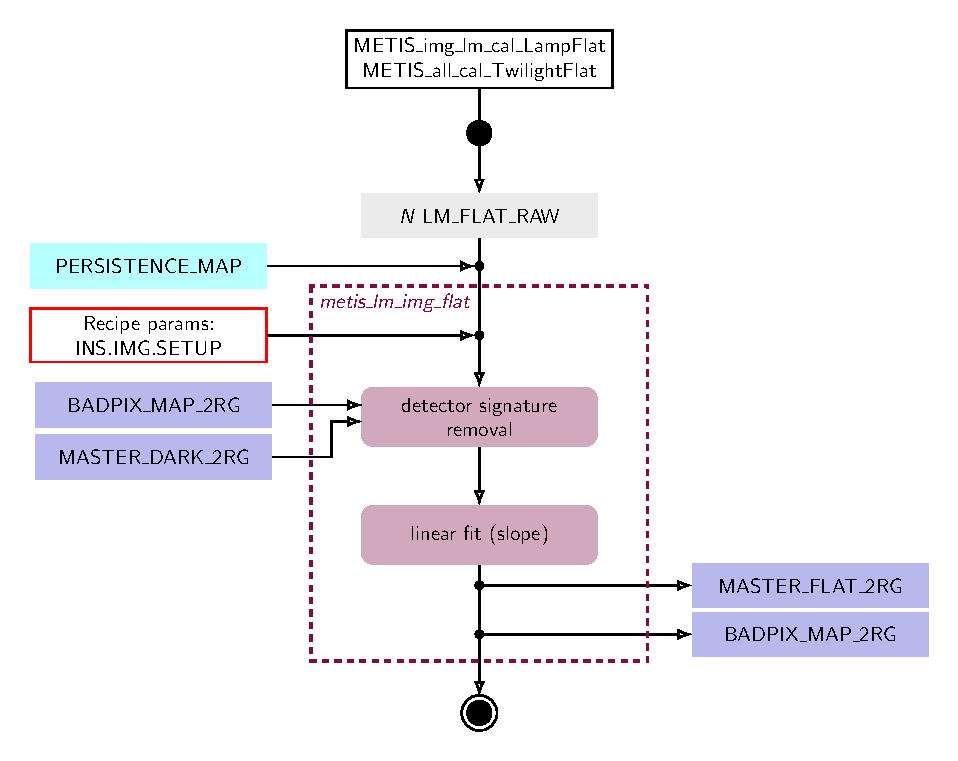
\includegraphics[width=0.6\textwidth]{metis_lm_img_flat}
  \caption[Recipe: \REC{metis_lm_img_flat}]{\REC{metis_lm_img_flat} --
    creation of \CODE{IMG_LM} master flatfield.\\ \TODO{Include averaging of
      frames at same illumination}}
  \label{fig:metis_lm_img_flat}
\end{figure}


\clearpage
\subsubsection{LM-band imaging basic reduction}
\label{lm_img_basic}
\label{rec:lm_img_basic}
\label{sssec:lm_img_basic}
\label{metis_lm_img_basic_reduce}
\label{rec:metis_lm_img_basic_reduce}
\label{sssec:metis_lm_img_basic_reduce}

\TODO{New recipe -- this may be too basic and could be joined with
  the background subtraction.}

This recipe performs the basic reduction of raw exposures from the
LM-band imager, i.e.\ dark subtraction, flat fielding and other removing
instrumental signals. It is used for both standard and science exposures.

Basic statistics of the images can be used to screen for saturation.

\TODO{This recipe should analyse the masked detector regions for
  channel offset correction and crosstalk (see \cite{matisse_minutes}).}

\begin{recipedef}
  Name:             & \REC{metis_lm_img_basic_reduce}   \\
  Purpose:          & apply basic reduction of images   \\
  Type:             & Calibration, Science              \\
  Templates:        & \TPL{METIS_img_lm_cal_standard}  \\
                    & \TPL{METIS_img_lm_*_obs_*}       \\
  Input data:       & Dithered images (standard, science) \\
                    & Blank sky images (if available)   \\
                    & Masked detector region (if available)  \\
                    & Master dark                       \\
                    & Master flat                       \\
  Matched keywords: & DIT (for dark)                    \\
                    & Filter ID (for flat)              \\
  Algorithm:        & Remove crosstalk, correct non-linearity \\
                    & Analyse and remove masked regions  \\
                    & Subtract dark, divide by flat       \\
                    & Remove blank sky pattern                \\
  Output data:      & \hyperref[dataitem:lm_sci_basic_reduced]{\PROD{LM_SCI_BASIC_REDUCED}}       \\
                    & \hyperref[dataitem:lm_std_basic_reduced]{\PROD{LM_STD_BASIC_REDUCED}}       \\
  QC1 parameters:   & \QC{QC LM IMG MEDIAN}             \\
                    & \QC{QC LM IMG STANDARD DEVIATION} \\
                    & \QC{QC LM IMG PEAK}               \\
  hdrl functions:   & \CODE{hdrl_imagelist_sub_image}   \\
                    & \CODE{hdrl_imagelist_div_image}   \\
\end{recipedef}

\begin{figure}[hb]
  \centering
  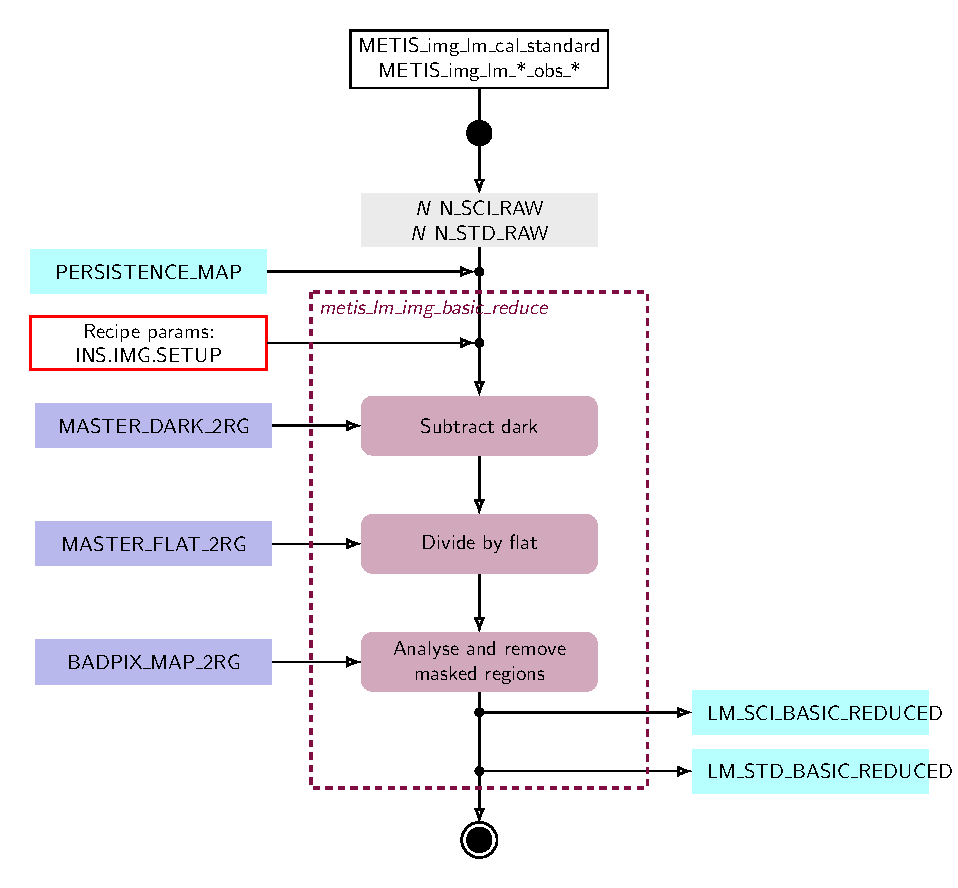
\includegraphics[width=0.6\textwidth]{metis_lm_img_basic_reduce}
  % \resizebox{0.6\textwidth}{0.1\textwidth}{\TODO{\fbox{Figure to be done}}}
  \caption[Recipe: \REC{metis_lm_img_basic_reduce}]{\REC{metis_lm_img_basic_reduce} --
    basic reduction of \CODE{IMG_LM} data.}
  \label{fig:metis_lm_img_basic_reduce}
\end{figure}


\clearpage
\subsubsection{LM-band imaging background subtraction}
\label{lm_img_background}
\label{rec:lm_img_background}
\label{sssec:lm_img_background}
\label{metis_lm_img_background}
\label{rec:metis_lm_img_background}
\label{sssec:metis_lm_img_background}

This recipe estimates and subtracts the background from LM-band
imaging data. Thermal background emission from the atmosphere,
telescope and warm parts of the instrument dominate the photon count
in mid-infrared observations. Accurate determination and removal of
background counts is therefore crucial to make MIR data scientifically
usable.

A set of observations will consist of a number of dithered exposures
of the field, where the offsets are achieved using the internal
chopper of METIS or the with the telescope. For extended objects, the
telescope will be used to perform ``out-of-field dithering'', i.e.\
observe nearby blank patches of sky interlaced with the target
observations. Imaging observations are performed in pupil-tracking
mode, hence angular dithering of the field is automatic.

For in-field-dithered exposures, all dithered exposures will be
averaged to obtain the background estimate. In order to only average
the background contribution, an iterative procedure of object
detection and masking will be employed. Averaging will be done using a
robust estimator of the mean (e.g.\ median).

For extended objects, all out-of-field exposures will be averaged
(with object rejection) and subtracted off the in-field exposures.

This fulfills \REQ{METIS-6085} and \REQ{METIS-6086}.

\TODO{Object catalogues of the target exposures could be created within this
recipe or in a separate recipe. The catalogue should contain for each
object: pixel coordinates ($x$, $y$), world coordinates ($\alpha$,
$\delta$) based on telescope pointing and derotator information, total
counts within an aperture.}

\TODO{Is this good enough for HCI images or do we need more?}

\begin{recipedef}
  Name:             & \REC{metis_lm_img_background}                             \\
  Purpose:          & estimate and subtract background                          \\
  Type:             & Calibration                                               \\
  Templates:        & \TPL{METIS_img_lm_cal_standard}                           \\
                    & \TPL{METIS_img_lm_*_obs_*}                                \\
  Input data:       & \hyperref[dataitem:lm_sci_basic_reduced]{\PROD{LM_SCI_BASIC_REDUCED}}                               \\
                    & \hyperref[dataitem:lm_std_basic_reduced]{\PROD{LM_STD_BASIC_REDUCED}}                               \\
  Matched keywords: & dither position (\CODE{SKY}? \TBD)                        \\
  Algorithm:        & Average all or \CODE{SKY} exposures with object rejection \\
                    & Subtract background                                       \\
  Output data:      & \hyperref[dataitem:lm_sci_bkg]{\PROD{LM_SCI_BKG}}                                         \\
                    & \hyperref[dataitem:lm_std_bkg]{\PROD{LM_STD_BKG}}                                         \\
                    & \hyperref[dataitem:lm_sci_bkg_subtracted]{\PROD{LM_SCI_BKG_SUBTRACTED}}                              \\
                    & \hyperref[dataitem:lm_std_bkg_subtracted]{\PROD{LM_STD_BKG_SUBTRACTED}}                              \\
                    & \hyperref[dataitem:lm_sci_object_cat]{\PROD{LM_SCI_OBJECT_CAT}}                                  \\
                    & \hyperref[dataitem:lm_std_object_cat]{\PROD{LM_STD_OBJECT_CAT}}                                  \\
  QC1 parameters:   & \QC{QC LM IMG BKG MEDIAN}                                 \\
                    & \QC{QC LM IMG BKG MEDIAN DEVIATION}                       \\
  hdrl functions:   & \CODE{hdrl_imagelist_sub_image}                           \\
                    & \CODE{hdrl_imagelist_div_image}                           \\
                    & \CODE{hdrl_catalogue_compute}                             \\
\end{recipedef}

\begin{figure}[hb]
  \centering
  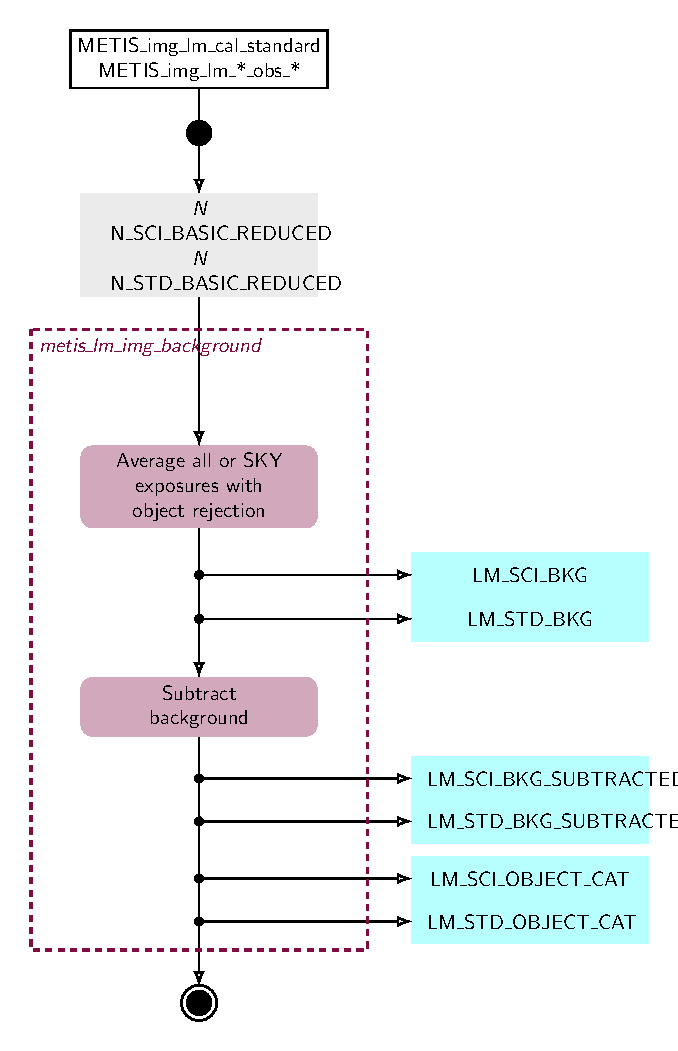
\includegraphics[width=0.6\textwidth]{metis_lm_img_background}
  % \resizebox{0.6\textwidth}{0.1\textwidth}{\TODO{\fbox{Figure to be done}}}
  \caption[Recipe: \REC{metis_lm_img_background}]{\REC{metis_lm_img_background} --
    background estimation and subtraction of dithered \CODE{IMG_LM} data.}
  \label{fig:metis_lm_img_background}
\end{figure}


\clearpage

% \subsubsection{LM-band imaging astrometry calibration}
%
% HB: I've commented the lm_img_astrometry_calib recipe out as it seems
%     not necessary. The two outputs as defined are:
%     - LM_STD_AST_CALIB: this is raw data produced by the
%       template METIS_img_lm_cal_standard, and thus should not be the
%       output of a recipe.
%     - ASTROMETRY_TAB: this seems equivalent to LM_DISTORTION_TABLE, or
%       at least very similar.
%
% \label{lm_img_astrometry_calib}
% \label{rec:lm_img_astrometry_calib}
% \label{sssec:lm_img_astrometry_calib}
% \label{metis_lm_img_astrometry_process}
% \label{rec:metis_lm_img_astrometry_process}
% \label{sssec:metis_lm_img_astrometry_process}
% This recipe is the conversion of the pixel coordinates (X,Y) of objects in an image
% into their corresponding celestial coordinates of right ascension (RA) and
% declination (Dec). The recipe for astrometry calibration involves several
% steps that must be carried out precisely to achieve accurate results.
%
% The first step of the recipe involves identifying a set of reference stars
% in the image, whose coordinates are well known and can be obtained from a
% catalog. This requires careful selection and verification of the reference stars,
% as their accuracy determines the accuracy of the final calibration.
%
% The next step is to use these reference stars to establish a mapping between
% the image's pixel coordinates and their corresponding celestial coordinates. This
% is achieved through a process called plate solving, which involves solving a set
% of mathematical equations to determine the transformation between pixel and celestial
% coordinates. This process requires careful selection of the appropriate transform function
% and calibration parameters.
%
% \begin{recipedef}
%   Name:                & \REC{metis_lm_img_astrometry_process}                                               \\
%   Purpose:             & Determine conversion factor between pixel and world coordinates              \\
%   Type:                & Calibration                                                                  \\
%   Templates:           & \TPL{METIS_img_lm_cal_standard}                                              \\
%   Input data:          & \hyperref[dataitem:lm_std_bkg_subtracted]{\PROD{LM_STD_BKG_SUBTRACTED}}                                                 \\
%                        & photometric standard catalogue                                               \\
%   Matched keywords:    & OBJECT ID                                                                    \\
%                        & FILTER ID                                                                    \\
%   Parameters:          & Distortion correction functions                                              \\
%   Algorithm:           & Measure position of stars in pixel coordinates                               \\
%                        & Compute conversion factor to world coordinates                               \\
%                        & Measure and evaluate the error.                                              \\
%   Output data:         & \hyperref[dataitem:lm_std_ast_calib]{\PROD{LM_STD_AST_CALIB}}                                                      \\
%                        & \hyperref[dataitem:astrometry_tab]{\PROD{ASTROMETRY_TAB}}                                                        \\
%   Expected accuracies: &  $>$0.1$\arcsec$                                                                    \\
%   QC1 parameters:      & \QC{QC LM AST X POS ERR}                                                     \\
%                        & \QC{QC LM AST Y POS ERR}                                                     \\
%                        & \QC{QC LM AST RA POS ERR}                                                    \\
%                        & \QC{QC LM AST DEC POS ERR}                                                    \\
%   hdrl function:       & \CODE{hdrl_strehl_compute}                                                   \\
%                        & \CODE{hdrl_catalogue_compute}                                                \\
%                        & \CODE{hdrl_efficiency_compute}                                               \\
%                        & \CODE{hdrl_imagelist_collapse}                                               \\
% \end{recipedef}
%
% \begin{figure}[hb]
%   \centering
%    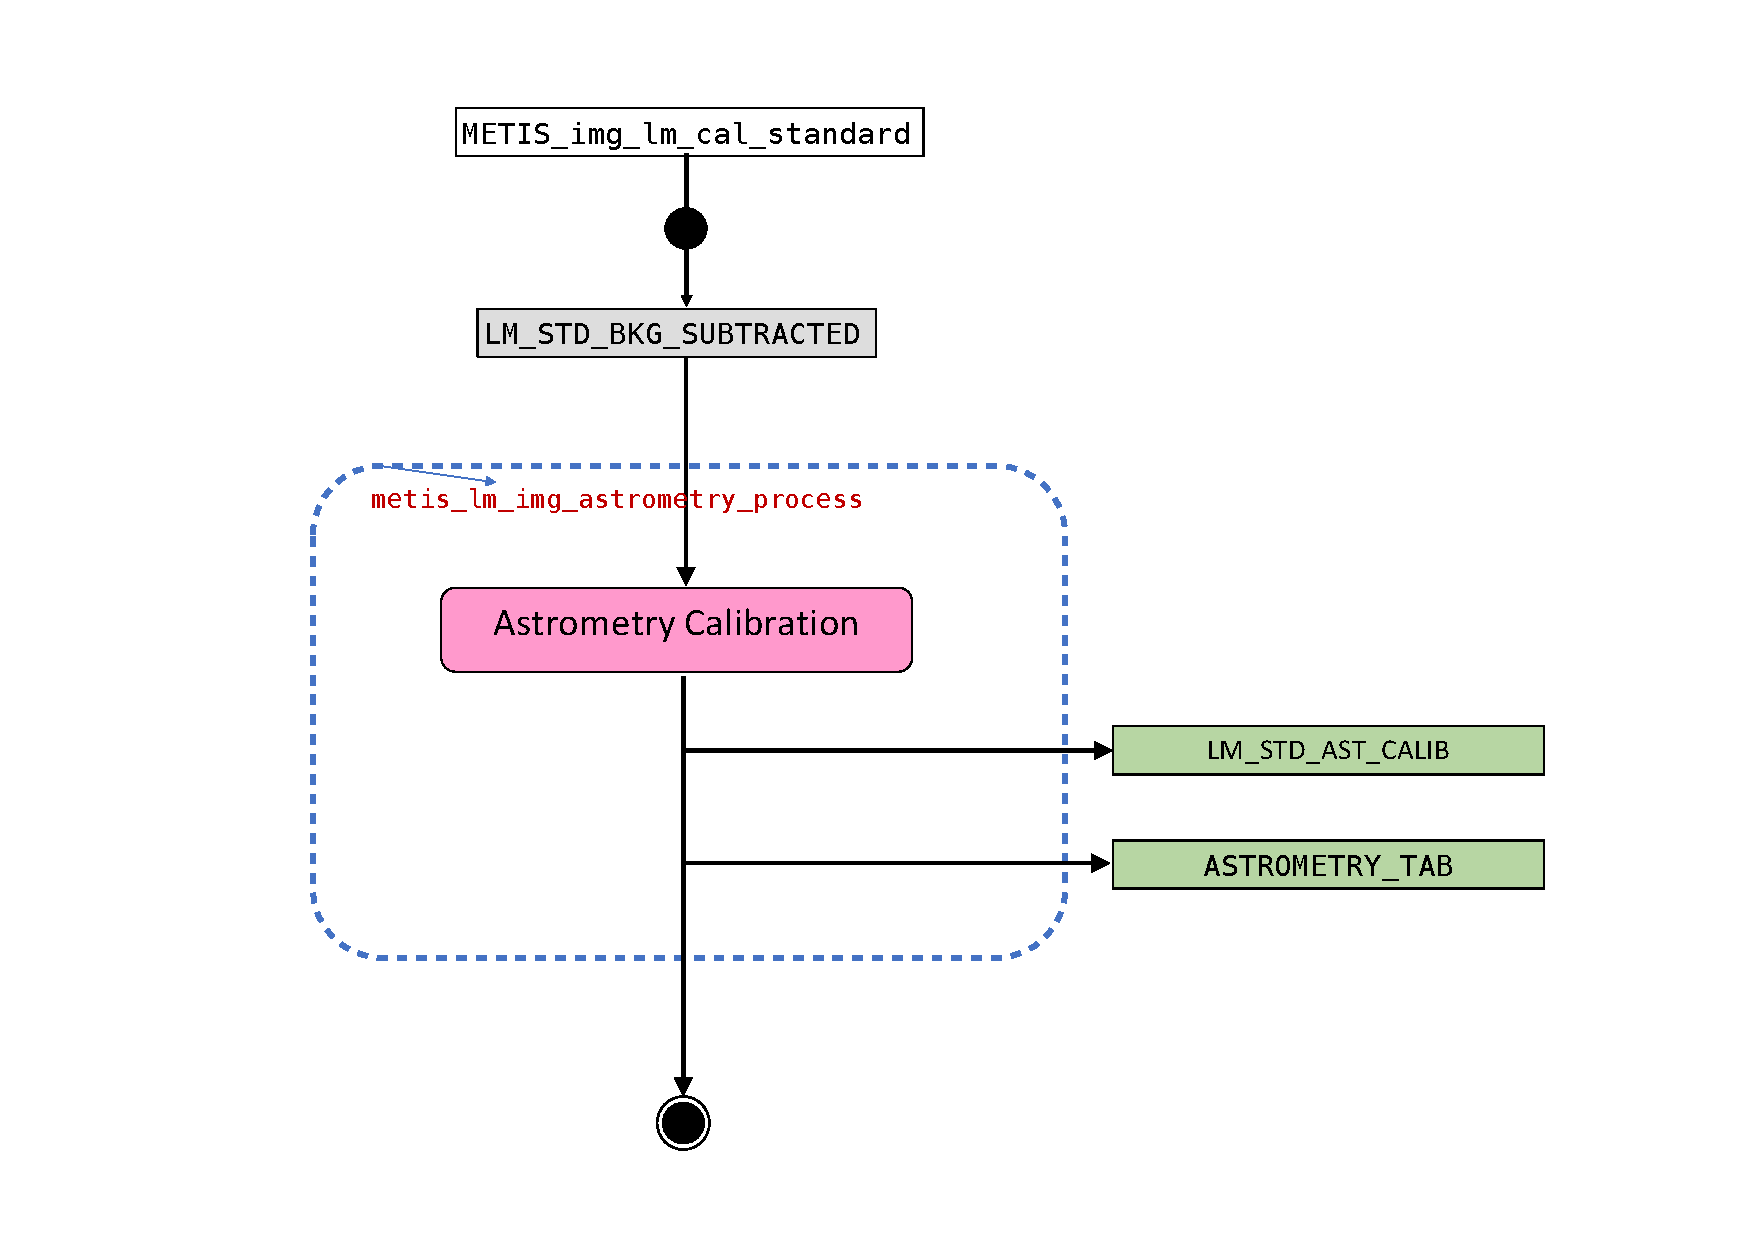
\includegraphics[width=1.0\textwidth]{metis_lm_img_astrometry_process}
%   %\resizebox{0.6\textwidth}{0.1\textwidth}{\TODO{\fbox{Figure to be done}}}
%   \caption[Recipe: \REC{metis_lm_img_astrometry_process}]{\REC{metis_lm_img_astrometry_process} --
%     compute conversion between pixel and sky coordinate}
%   \label{fig:metis_lm_img_astrometry_process}
% \end{figure}
%
%
% \clearpage

\subsubsection{LM-band imaging photometric standard analysis}
\label{lm_img_photstd}
\label{rec:lm_img_photstd}
\label{sssec:lm_img_photstd}

This recipe determines the conversion from ADU to physical units from
a set of reduced exposures of a photometric standard star. The flux of
the star is measured in each exposure in ADU, normalised to an
exposure time of 1~second and averaged over all exposures. In
addition, the exposures are stacked (after recentering on the standard
star, but without derotation) and the flux is measured in the combined
image. Comparison to the tabulated brightness of the star in the
observing filter yields the conversion factor from
$\mathrm{ADU\,s^{-1}}$ to $\mathrm{photons\,\,s^{-1}\,cm^{-2}}$.

QC parameter will include estimates of the sensitivity for the
detection of point sources and surface brightness sensitivity
following \cite{visir_manual}.

\begin{recipedef}\label{rec:metis_lm_img_std_process}
  Name:                & \REC{metis_lm_img_std_process}                                               \\
  Purpose:             & Determine conversion factor between detector counts and physical source flux \\
  Type:                & Calibration                                                                  \\
  Templates:           & \TPL{METIS_img_lm_cal_standard}                                              \\
  Input data:          & \hyperref[dataitem:lm_std_bkg_subtracted]{\PROD{LM_STD_BKG_SUBTRACTED}}                                                 \\
                       & photometric standard catalogue                                               \\
  Matched keywords:    & OBJECT ID                                                                    \\
                       & FILTER ID                                                                    \\
  Parameters:          & None (TBD)                                                                   \\
  Algorithm:           & Call \DRL{calculate_std_flux} to measure flux in input images                      \\
                       & call \DRL{recentre_img} to recentre and stack images                         \\
                       & call \DRL{calculate_std_flux} on the stacked image to get flux of the star in detector units\\
                       & call \DRL{caluculate_std_fluxcal} to calculate the conversion factor to physical units    \\
                       & call \DRL{calculate_detection_limits} to compute measure background noise (std,rms) and compute detection limits \\
  Output data:         & \hyperref[dataitem:lm_std_combined]{\PROD{LM_STD_COMBINED}}                                                       \\
                       & \hyperref[dataitem:fluxcal_tab]{\PROD{FLUXCAL_TAB}}                                                           \\
  Expected accuracies: & \TBD                                                                         \\
  QC1 parameters:      & \QC{QC LM IMG STD BACKGD RMS}                                                \\
                       & \QC{QC LM STD PEAK CNTS}                                                     \\
                       & \QC{QC LM STD APERTURE CNTS}                                                 \\
                       & \QC{QC LM STD STREHL}                                                        \\
                       & \QC{QC LM STD FLUXCONV}                                                      \\
                       & \QC{QC LM STD AIRMASS}                                                       \\
                       & \QC{QC LM SENSITIVITY}                                                       \\
                       & \QC{QC LM AREA SENSITIVIY}                                                   \\
  hdrl functions:      & \CODE{hdrl_strehl_compute}                                                   \\
                       & \CODE{hdrl_catalogue_compute}                                                \\
                       & \CODE{hdrl_efficiency_compute}                                               \\
                       & \CODE{hdrl_imagelist_collapse}                                               \\
\end{recipedef}

\begin{figure}[hb]
  \centering
   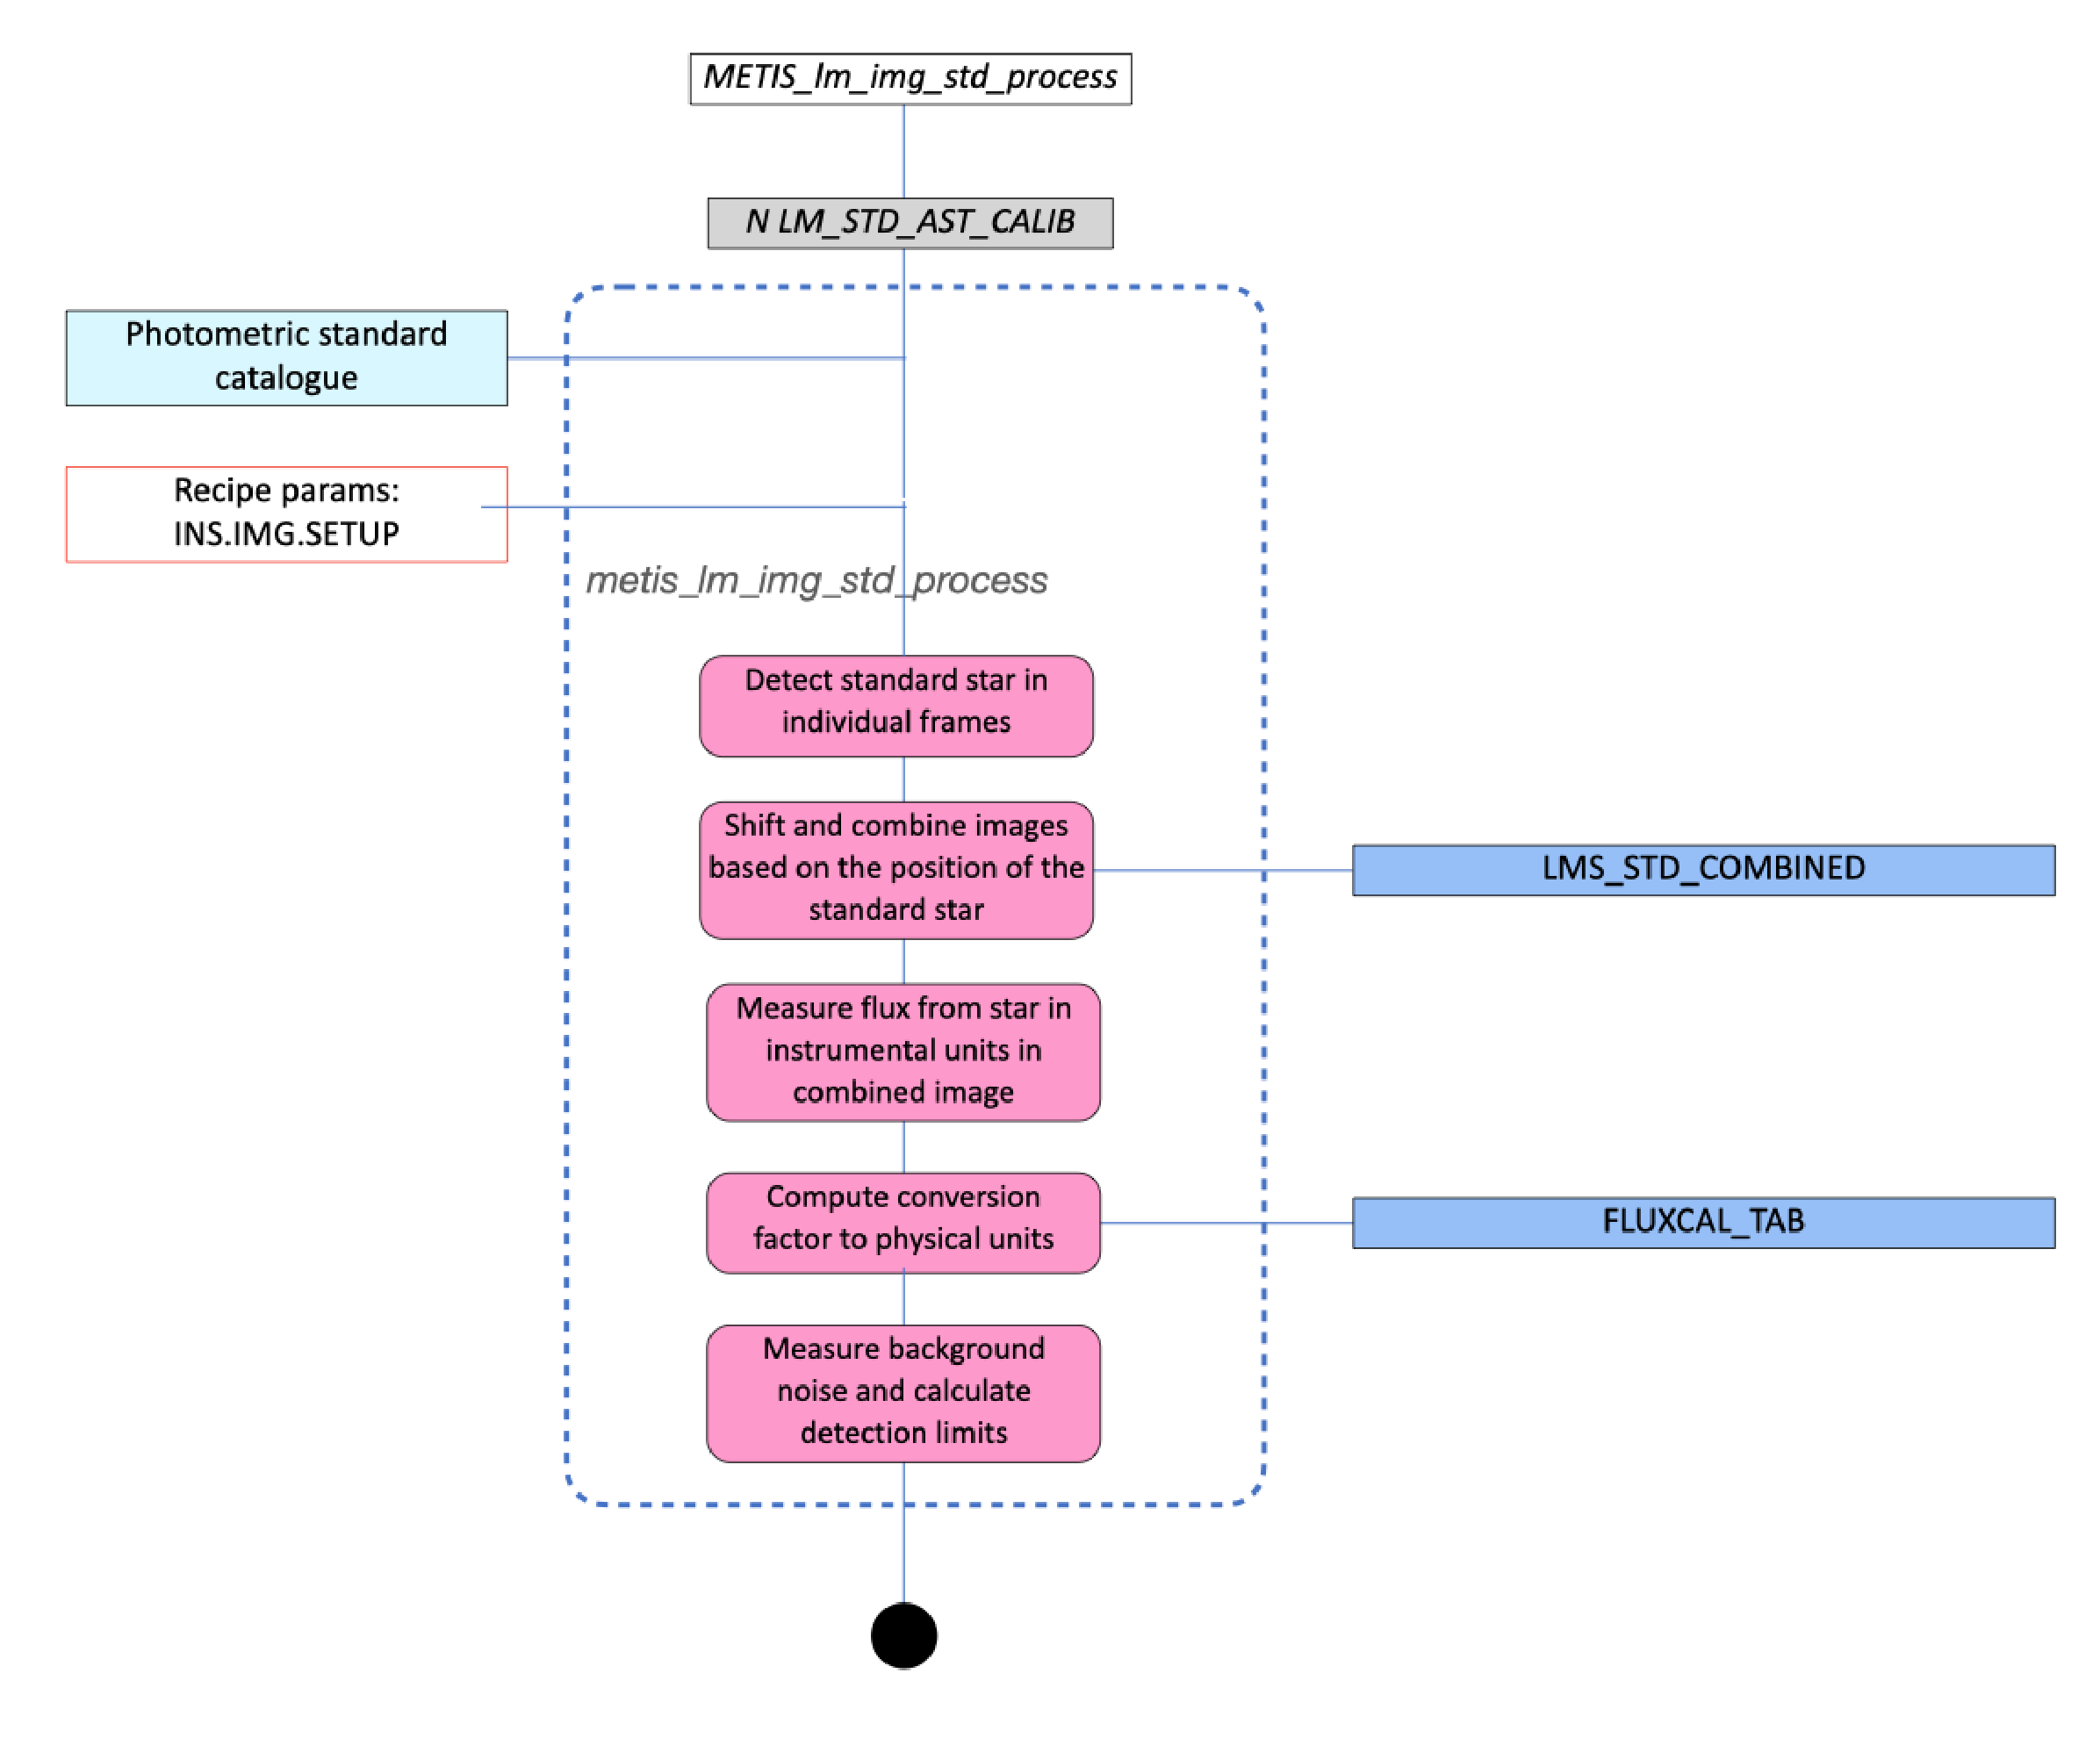
\includegraphics[width=0.6\textwidth]{metis_lm_img_std_process}
  %\resizebox{0.6\textwidth}{0.1\textwidth}{\TODO{\fbox{Figure to be done}}}
  \caption[Recipe: \REC{metis_lm_img_std_process}]{\REC{metis_lm_img_std_process} --
    compute conversion between ADU and physical flux units}
  \label{fig:metis_lm_img_std_process}
\end{figure}

%%%%%%%%%%%%%%%%%%%%%%%%%%%%%%%%%%%%%%%%%%%%%%%%%

\clearpage
\subsubsection{LM-band imaging calibration}
\label{lm_img_calibrate}
\label{rec:lm_img_calibrate}
\label{sssec:lm_img_calibrate}

This recipe applies the flux calibration to the reduced science
images and adds geometric calibration data to the FITS header. The
products of this recipe are fully calibrated individual exposures.

Each image is multiplied by the conversion factor such that pixel
values are in units of photons per second per centimetre squared. The
header of each file receives keyword \FITS{BUNIT} with value %
\CODE{'photon.s**(-1).cm**(-2)'}.

\TODO{Other units may be possible, although additional information is
  needed. For instance,\\ \CODE{photon.s**(-1).cm**(-2).arcsec**(-2)} makes
  values independent of the pixel scale, but requires a distortion map
  (variation of pixel scale across the detector). Energy units (erg
  instead of photons) require knowledge of the spectral energy
  distribution of the sources, in particular for broad-band filters.}

LM-band imaging observations will be performed in pupil-tracking mode
\cite{METIS-operational_concept}, which means that the field rotates
from exposure to exposure.  The information about the field
orientation along with target coordinates, pixel scale and
higher-order polynomial distortion coefficients is written to the FITS
header. The images are not resampled by this recipe, this is left to
\REC{metis_lm_img_sci_postprocess}.



\begin{recipedef}\label{rec:metis_lm_img_calibrate}
  Name:              & \REC{metis_lm_img_calibrate}                     \\
  Purpose:           & Convert science images to physical units         \\
                     & Add distortion information                       \\
  Type:              & Calibration                                      \\
  Templates          & ??                                                 \\
  Input data:        & \hyperref[dataitem:lm_sci_bkg_subtracted]{\PROD{LM_SCI_BKG_SUBTRACTED}}                     \\
                     & \hyperref[dataitem:fluxcal_tab]{\PROD{FLUXCAL_TAB}}                               \\
                     & \hyperref[dataitem:lm_distortion_table]{\PROD{LM_DISTORTION_TABLE}}                       \\
  Matched keywords:  & Filter ID                                        \\
  Parameters:        & None (TBD)                                       \\
  Algorithm:         & call \DRL{lm_scale_image_flux} to Scale image data to ph/s \\
                     & call \DRL{lm_add_header_distortion} to add header information (\FITS{BUNIT}, WCS, etc.) \\
  Output data:       & \hyperref[dataitem:lm_sci_calibrated]{\PROD{LM_SCI_CALIBRATED}}                         \\
  QC1 parameters:    & None                                             \\
  hdrl functions:    & \CODE{hdrl_imagelist_mult_scalar}                \\
\end{recipedef}

\begin{figure}[hb]
  \centering
  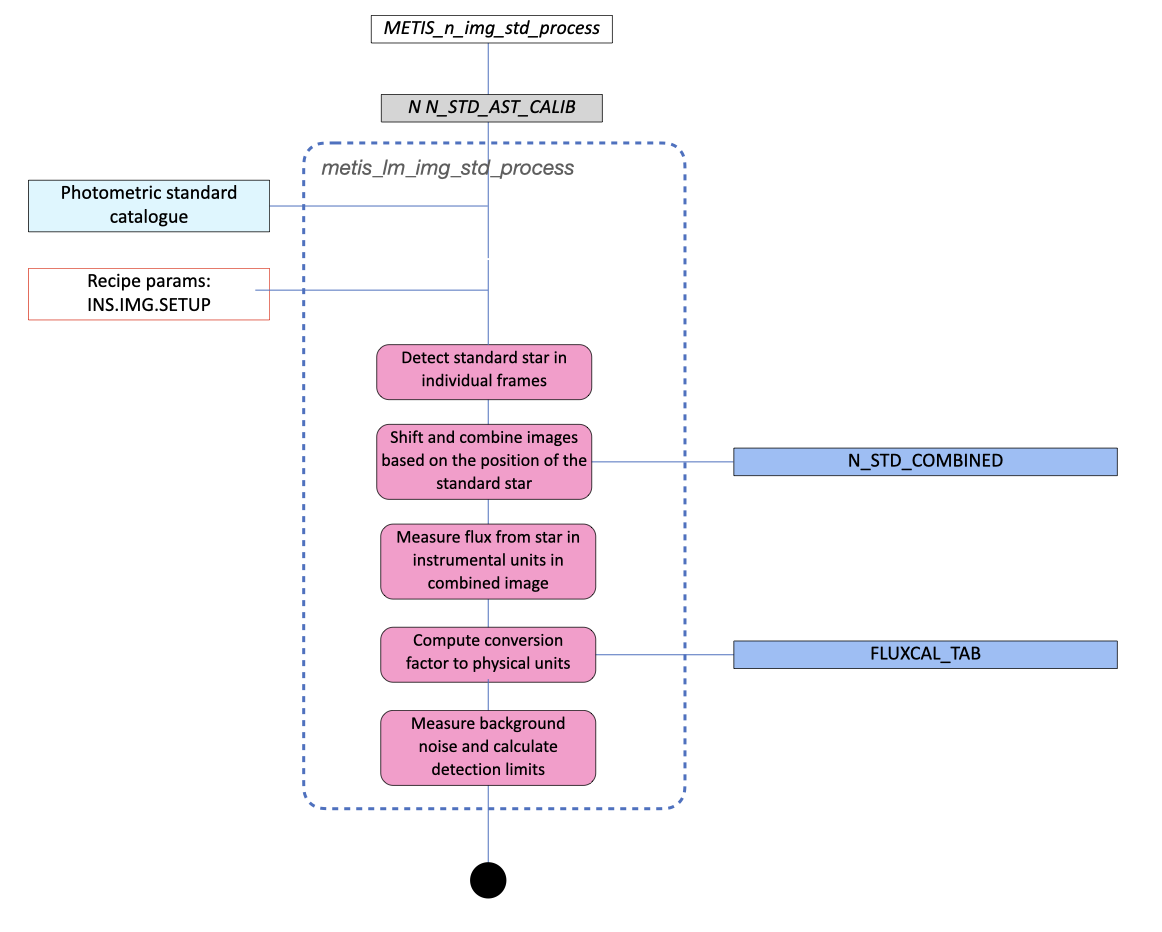
\includegraphics[width=0.6\textwidth]{lm_img_calibrate}
  \caption[Recipe: \REC{metis_lm_img_calibrate}]{\REC{metis_lm_img_calibrate} --
    Convert images to physical flux units and update FITS header}
  \label{fig:metis_lm_img_calibrate}
\end{figure}


%%%%%%%%%%%%%%%%%%%%%%%%%%%%
\clearpage
\subsubsection{LM-band imaging post-processing}
\label{lm_img_postprocess}
\label{rec:lm_img_postprocess}
\label{sssec:lm_img_postprocess}

This recipe coadds a sequence of flux-calibrated,
background-subtracted images (possibly from several observing blocks)
after resampling the images on a common pixel grid defined by a
standard sky projection. The alignment of the images (\FITS{CRVAL}
keywords, rotation) may have to be checked and refined through
cross-correlation of the overlapping images (TBC). The number of input
images contributing to any pixel in the output image (variable due to
dither offsets and bad pixels) will be documented in a contribution
map.

This recipe will only be used in the science-grade pipelines, not at
the observatory. The output fulfills the criteria for \ac{SDP}s and is compliant with \REQ{METIS-6104}.

\begin{recipedef}\label{rec:lm_img_flat}
  Name:                & \REC{metis_lm_img_sci_postprocess}                         \\
  Purpose:             & Coadd reduced images.                                      \\
  Requirements:        & \REQ{METIS-6104}                                           \\
  Templates:           & ---                                                        \\
  Type:                & Science                                                    \\
  Input data:          & Calibrated science images (\PROD{LM_SCI_CALIBRATED})       \\
                       & Associated bad-pixel maps (\PROD{BADPIX_MAP_LM})           \\
  Parameters:          & None (TBD).                                                \\
  Algorithm:           & Check and refine WCS of input images by cross-correlation  \\
                       & \hspace{1em} (on object catalogue or on image).            \\
                       & Determine output pixel grid encompassing all input images. \\
                       & Resample images to output pixel grid.                      \\
                       & Coadd.                                                     \\
  Output data:         & \hyperref[dataitem:lm_sci_coadd]{\PROD{LM_SCI_COADD}} (coadded, mosaiced image)              \\
% TheLM_SCI_COADD_ERROR and LM_SCI_COADD_CONTRIB can be layers in LM_SCI_COADD
%                        & \hyperref[dataitem:lm_sci_coadd_error]{\PROD{LM_SCI_COADD_ERROR}} (coadded, mosaiced error image)  \\
%                        & \hyperref[dataitem:lm_sci_coadd_contrib]{\PROD{LM_SCI_COADD_CONTRIB}} (contribution map)             \\
  Expected accuracies: & TBD                                                        \\
  QC1 parameters:      & \QC{QC LM SCI NEXPOSURE}                                   \\
\end{recipedef}

\begin{figure}[hb]
  \centering
  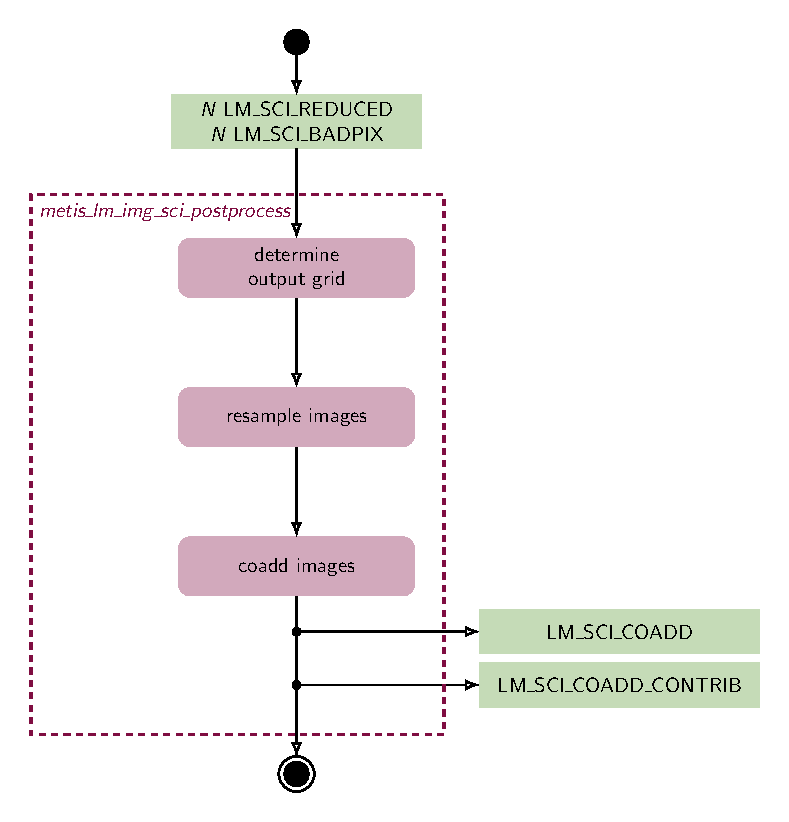
\includegraphics[width=0.7\textwidth]{metis_lm_img_sci_postprocess}
  \caption[Recipe: \REC{metis_lm_img_sci_postprocess}]{%
    \REC{metis_lm_img_sci_postprocess} -- post-processing (coaddition)
    of reduced \CODE{IMG_LM} science frames.}
  \label{fig:metis_lm_img_sci_postprocess}
\end{figure}

%%%%%%%%%%%%%%%%%%%%%%%%%%%%%%%%%%%%%%%%%%%%
\clearpage
\subsubsection{LM-band imaging distortion calibration}
\label{rec:metis_lm_img_distortion}
\label{lm_img_distortion}
\label{rec:lm_img_distortion}
\label{sssec:lm_img_distortion}

Calibration of the imaging distortion is done on an image of a
pin-hole grid mask located in a focal plane within the instrument. The
distortion is described in terms of a polynomial model whose
coefficients can be transformed to WCS keywords and applied to any
other pipeline product. In addition to the distortion table, a map of
pixel scale across the detector will be created.

\begin{recipedef}
  Name:                & \REC{metis_lm_img_distortion}                                   \\
  Purpose:             & Determine optical distortion coefficients for the LM imager.    \\
  Requirements:        & \REQ{METIS-6087}                                                \\
  Templates:           & \TPL{METIS_img_lm_cal_distortion}                               \\
  Type:                & Calibration                                                     \\
  Input data:          & Images of grid mask in WCU-FP2 or CFO-FP2.                      \\
                       & Image with WCU window closed (background)                       \\
                       & Grid of pinhole mask positions \\
                       & Bad pixel map                                                  \\
  Parameters:          & Parameters for fitting routine      \\
                       & \TBD \\
  Algorithm:           & Subtract background image.    (\CODE{hdrl_imagelist_sub_image})                                  \\
                       & Measure location of point source images in frames (\CODE{hdrl_catalogue_create})             \\
                       & call \hyperref[drl:fit_distortion]{\CODE{fit_distortion}} to fit polynomial coefficients to deviations from grid positions.  \\
  Output data:         & \hyperref[dataitem:lm_distortion_table]{\PROD{LM_DISTORTION_TABLE}} \\
                       & \hyperref[dataitem:lm_distortion_map]{\PROD{LM_DISTORTION_MAP}}        \\
                       & \hyperref[dataitem:lm_dist_reduced]{\PROD{LM_DIST_REDUCED}}               \\
  Expected accuracies: & TBD                                                             \\
  QC1 parameters:      & \hyperref[qc:qc_lm_distort_rms]{\QC{QC LM DISTORT RMS}}                                          \\
                       & \hyperref[qc:qc_lm_distort_nsource]{\QC{QC LM DISTORT NSOURCE}}  \\
  hdrl functions:      & \CODE{hdrl_catalogue_create}                                    \\
                       & \CODE{hdrl_imagelist_sub_image}                                \\
\end{recipedef}

\begin{figure}[hb]
  \centering
  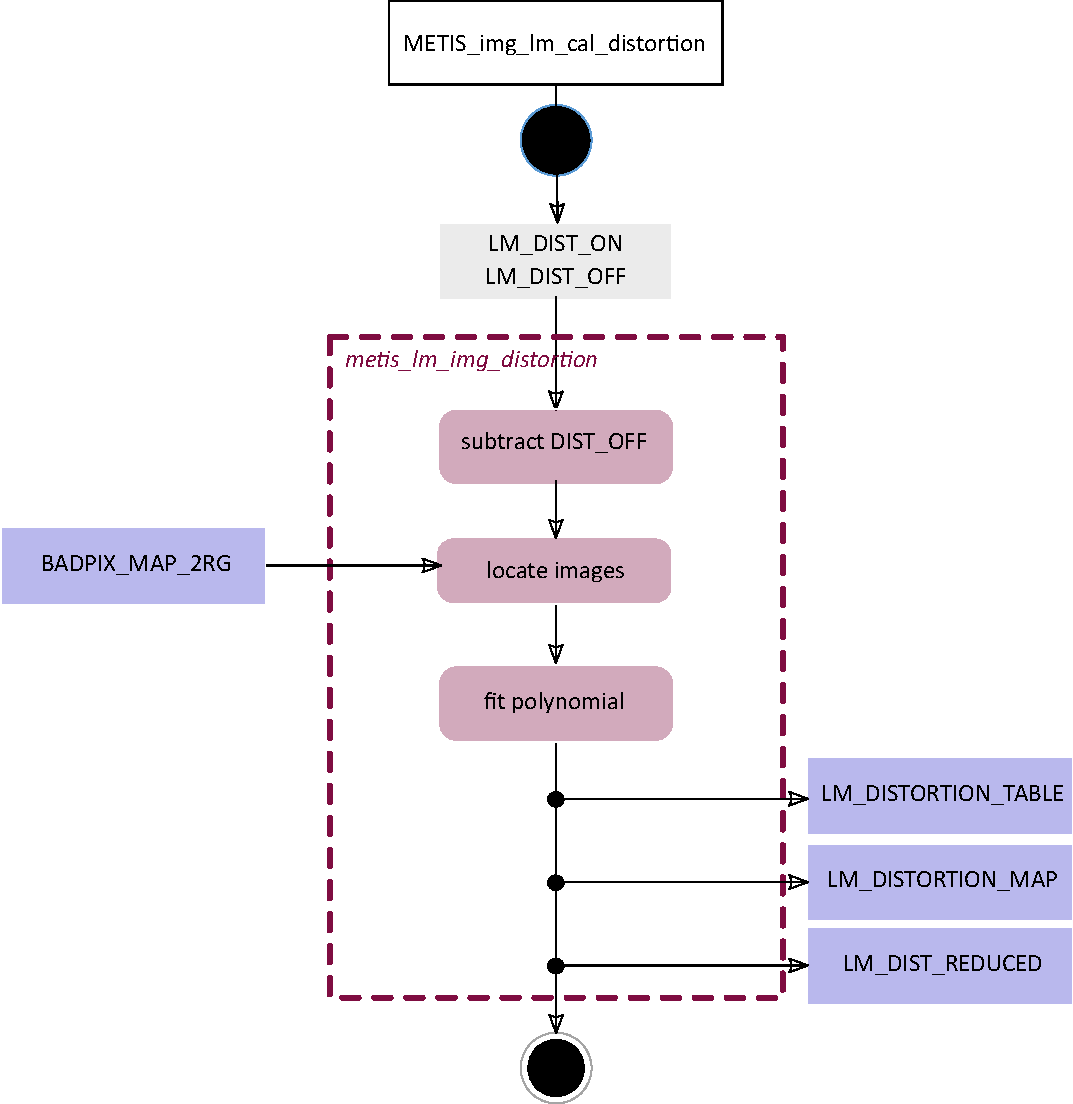
\includegraphics[width=0.6\textwidth]{metis_lm_img_distortion}
  \caption[Recipe: \REC{metis_lm_img_distortion}]{%
    \REC{metis_lm_img_distortion} -- LM IMG distortion calibration}
  \label{fig:metis_lm_img_distortion}
\end{figure}

\FloatBarrier

%%% Local Variables:
%%% TeX-master: "METIS_DRLD"
%%% End:


\subsection{N-band imaging}
\label{ssec:recipes_img_n}

\subsubsection{N-band imaging flatfield}
\label{n_img_flatfield}
\label{rec:n_img_flatfield}
\label{sssec:n_img_flatfield}
\label{n_img_flat}
\label{rec:n_img_flat}
\label{sssec:n_img_flat}
\label{metis_n_img_flat}
\label{rec:metis_n_img_flat}
\label{sssec:metis_n_img_flat}

The purpose of the flat-field calibration is to determine
pixel-to-pixel gain variations and large scale illumination variations
(due to inhomogeneities of optical elements in the telescope or
instrument). Calibration frames are obtained either during day time
using the black-body lamp of the \ac{WCU} (internal flats) or by taken
images of the twilight sky (twilight flats). Advantages and
disadvantages of the two types of flat are discussed in
\cite{METIS-calibration_plan}.

MIR detectors are typically unstable in that they show gain
fluctuations on rather short time scales, hence science exposures may
have a different flat-field structure from those captured by the
calibration flats.  While the GeoSnap detector is expected to be more
stable than the AQUARIUS detector, its stability properties need to be
studied further in order to assess whether science images can be flat
fielded.  N-band flat fields will be taken in any case for quality
control and monitoring purposes.

Since the operational concept for twilight flats needs to be refined
during commissioning at the telescope, the current recipe design is
primarily valid for internal flats.

This recipe creates a master flat for the GeoSnap detector (N-band
imaging) from lamp or sky images matched by various setup parameters
as detailed below.  A set of internal flats includes a number of
exposures with \CODE{LAMP OFF}, which will be used for dark
subtraction. For twilight flats a master dark will be subtracted. The
master flat is obtained by the slope of a linear fit of the pixel
values against the illumination level of the exposures.

The quality control parameters give various statistics for each input
frame (mean, standard deviation, etc.), the standard deviation of the
normalised master flat and the number of bad pixels identified by the
recipe. If a bad-pixel map is provided on input, it is updated,
otherwise a new one is created.

\begin{recipedef}
  Name:                & \REC{metis_n_img_flat}                                         \\
  Purpose:             & Create master flat field for the N-band imaging detector.      \\
  Requirements:        & \REQ{METIS-6098}                                               \\
  Type:                & Calibration                                                    \\
  Templates:           & \TPL{METIS_img_n_cal_InternalFlat}                             \\
                       & \TPL{METIS_img_n_cal_TwilightFlat}                               \\
  Input data:          & Flat field images taken with lamp or sky.                      \\
                       & Master dark (for twilight flats)                               \\
                       & Bad pixel map                                                  \\
  Matched keywords:    & Detector ID                                                    \\
                       & Filter ID                                                      \\
                       & ADC ID                                                         \\
                       & Flat type (internal or twilight)                               \\
                       & possibly others (e.g.\ coronagraphic mask, \TBD)               \\
  Parameters:          & Combination method (\texttt{mean}, \texttt{median},
                         \texttt{sigclip}, \dots)                                       \\
                       & Parameters for combination methods                             \\
                       & Threshold(s) for deviant-pixel identification                  \\
  Algorithm:           & Call \REC{metis_apply_persistance_correction} to apply the
                         persistance correction \\
                       & For internal flats: call \REC{metis_det_dark} with \CODE{LAMP OFF}
                       images to create dark frame. \\
                       & Subtract internal dark or master dark from flat exposures.     \\
                       & call \REC{metis_n_img_flat} to fit slope of pixel values against
                       illumination level. Frames with the same exposure time will be averaged.\\
                       & Compute median or average of input frames to improve statistics.\\
                       & Call \REC{metis_update_lm_flat_mask} to flag deviant pixels. \\
  Output data:         & \PROD{MASTER_IMG_FLAT_N}                                       \\
                       & \PROD{BADPIX_MAP_N}                                            \\
  Expected accuracies: & \TBD                                                           \\
  QC1 parameters:      & \QC{QC N MASTERFLAT RMS}                                       \\
                       & \QC{QC N FLAT NBADPIX}                                         \\
                       & \QC{QC N FLAT MEAN ##}                                         \\
                       & \QC{QC N FLAT RMS ##}                                          \\
  hdrl functions:      & \CODE{hdrl_bpm_fit_compute}                                    \\
                       & \CODE{hdrl_imagelist_collapse}                                 \\
                       & \CODE{hdrl_imagelist_sub_image}                                \\
\end{recipedef}

\begin{figure}[hb]
  \centering
  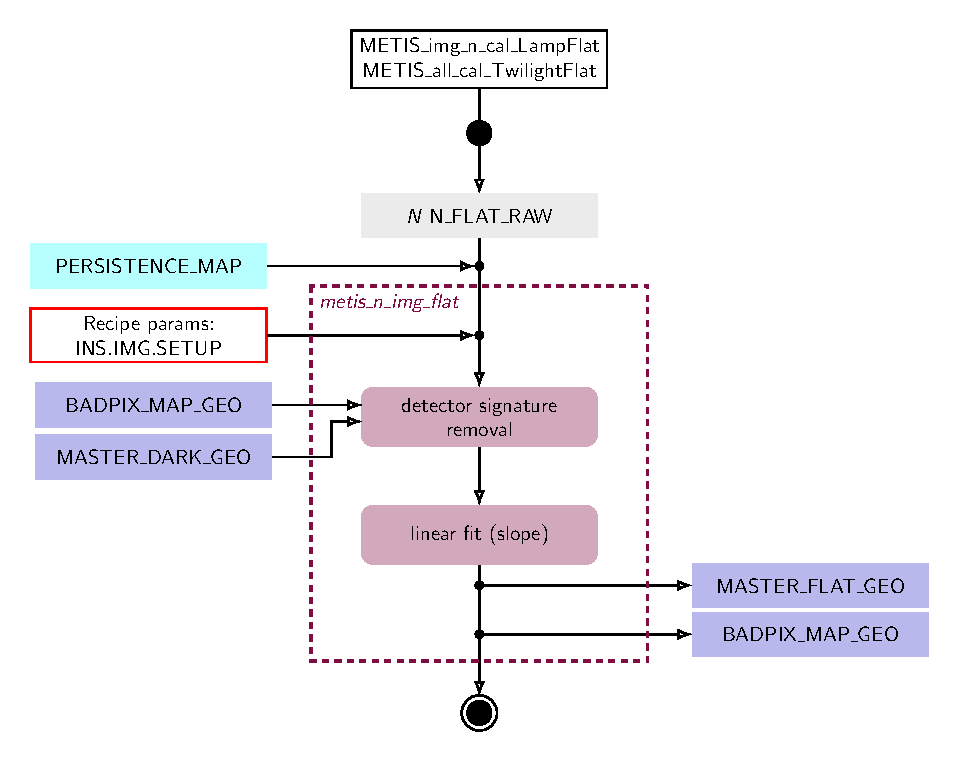
\includegraphics[width=0.6\textwidth]{metis_n_img_flat}
  \caption[Recipe: \REC{metis_n_img_flat}]{\REC{metis_n_img_flat} --
    creation of \CODE{IMG_N} master flatfield}
  \label{fig:metis_n_img_flat}
\end{figure}

%%%%%%%

\subsubsection{N-band imaging chop-nod combination}
\label{img_n_chopnod}
\label{rec:img_n_chopnod}
\label{rec:metis_n_img_chopnod}
\label{sssec:img_n_chopnod}

This recipe combines a set of exposures taken at all positions of a
defined chop-nod pattern and adds/subtracts them into a single
chop/nod difference image. Depending on the actual chop-nod pattern,
this image will contain one or more positive and negative beams.

If flat fielding proves feasible and useful for the GeoSnap detector
the master flat can be applied. If no jitter is applied, i.e.\ if the
beam is at the same detector position for all exposures taken at a
given chop position, then the master flat can be divided into the
final chop-nod difference image. Otherwise, the master flat will have
to be divided into the chop half-cycle images before the jitter
correction is applied.

\begin{recipedef}
  Name:              & \REC{metis_n_img_chopnod}                                    \\
  Purpose:           & chop/nod combination of exposures for background subtraction \\
  Type:              & Calibration, Science                                         \\
 Templates:          & \TPL{METIS_img_n_cal_standard}                              \\
                     & \TPL{METIS_img_n_obs_AutoChopNod}                            \\
                     & \TPL{METIS_img_n_obs_GenericChopNod}                         \\
                     & \TPL{METIS_img_n_cvc_obs_AutoChop}                           \\
%                     & \TPL{METIS_img_n_clc_obs_FixedSkyOffset}                     \\
                     & \TPL{METIS_img_n_cal_psf}                                    \\
  Input data:        & Chopped/nodded science or standard images                    \\
                     & Bad-pixel map                                                \\
  Matched keywords:  & Filter ID                                                    \\
                     & Chop position                                                \\
                     & Nod position                                                 \\
  Parameters:        & TBD                                                          \\
  Algorithm:         & Add/subtract images to subtract background                   \\
  Output data:       & \PROD{N_SCI_BKG_SUBTRACTED}                                  \\
                     & \PROD{N_STD_BKG_SUBTRACTED}                                  \\
  QC1 parameters:    & \QC{N IMG PEAK CNTS}                                         \\
  hdrl functions:    & \CODE{hdrl_imagelist_collapse}                               \\
\end{recipedef}

\begin{figure}[hb]
  \centering
   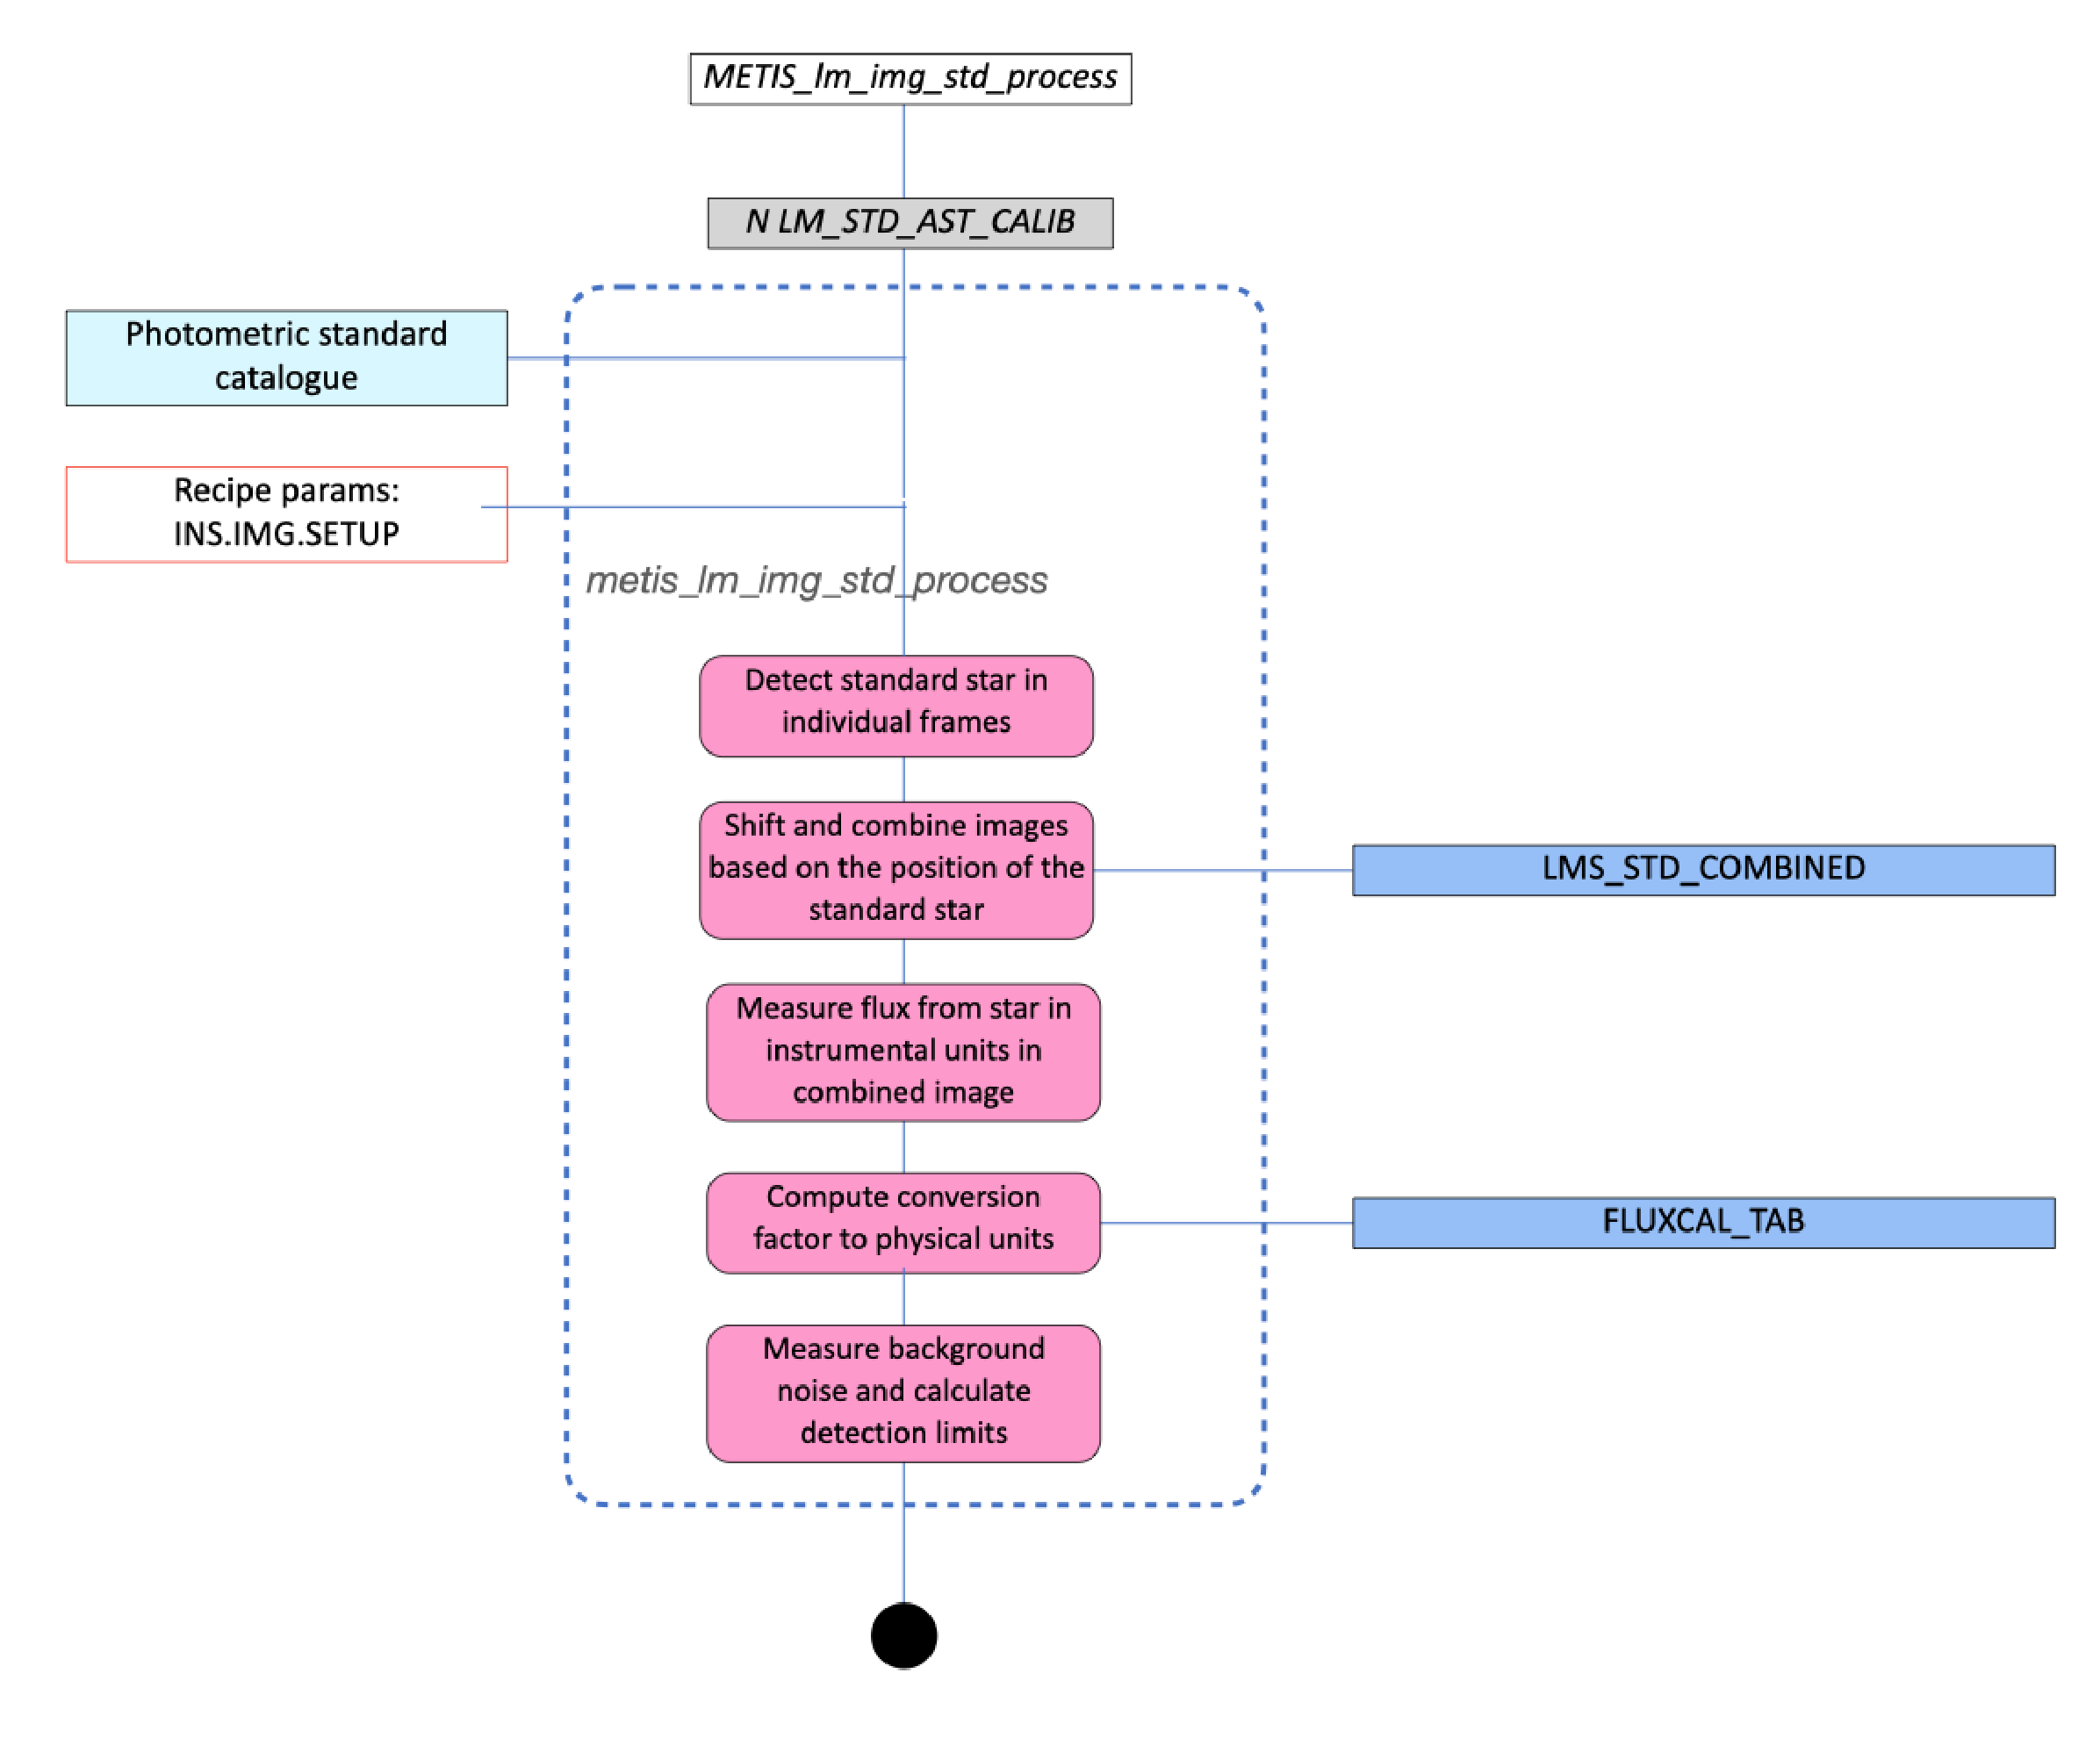
\includegraphics[width=0.6\textwidth]{metis_lm_img_std_process}
  \resizebox{0.6\textwidth}{0.1\textwidth}{\TODO{\fbox{Figure to be done}}}
  \caption[Recipe: \REC{metis_n_img_chopnod}]{\REC{metis_n_img_chopnod} --
    Combination of chop/nodded images.}
  \label{fig:metis_n_img_chopnod}
\end{figure}

%%%%%%%%%%%%%%%%%%%
\clearpage
\subsubsection{N-band imaging photometric standard analysis}
\label{n_img_std_process}
\label{rec:n_img_std_process}
\label{ssec:n_img_std_process}
\label{sssec:n_img_std_process}
\label{metis_n_img_std_process}
\label{rec:metis_n_img_std_process}
\label{sssec:metis_n_img_std_process}

This recipe determines the conversion from ADU to physical units from
a chop-nod difference image of a photometric standard star.  The flux
of the standard star is measured in each of the beams of the chop-nod
difference image, averaged and normalised to an exposure time of
1~second. Comparison to the tabulated brightness of the star in the
observing filter yields the conversion factor from
$\mathrm{ADU}\,\mathrm{s}^{-1}$ to
$\mathrm{photons}\,\mathrm{s}^{-1}\,\mathrm{cm}^{-2}$.

QC parameters will include estimates of the sensitivity for the
detection of point sources and surface brightness sensitivity
following \cite{visir_manual}.

\begin{recipedef}
  Name:                & \REC{metis_n_img_std_process}                                                 \\
  Purpose:             & Determine conversion factor between detector counts and physical source flux. \\
  Type:                & Calibration                                                                   \\
  Templates:           & \TPL{METIS_img_n_cal_standard}                                                \\
  Input data:          & \CODE{N_STD_BKG_SUBTRACTED}                                                   \\
                       & photometric standard catalogue                                                \\
  Matched keywords:    & Object ID                                                                     \\
                       & Filter ID                                                                     \\
  Parameters:          & None (TBD)                                                                    \\
  Algorithm:           & call \CODE{n_calculate_std_flux} to measure the flux in all beams\\
                       & average and normalize flux values \\
                       & call \CODE{calculate_std_fluxcal} to calculate conversion factor to physical units   \\
                       & call \CODE{calculate_detection_limits} to compute measured background noise (std, rms) and compute detection limits \\
  Output data:         & \PROD{FLUXCAL_TAB}                                                            \\
  Expected accuracies: & \TBD                                                                          \\
  QC1 parameters:      & \QC{QC N STD PEAK CNTS}                                                       \\
                       & \QC{QC N STD APERTURE CNTS}                                                   \\
                       & \QC{QC N STD STREHL}                                                          \\
                       & \QC{QC N STD FLUXCONV}                                                        \\
                       & \QC{QC N STD AIRMASS}                                                         \\
                       & \QC{QC N SENSITIVITY}                                                         \\
                       & \QC{QC N AREA SENSITIVITY}                                                    \\
  hdrl functions:      & \CODE{hdrl_catalogue_create}                                                  \\
                       & \CODE{hdrl_strehl_compute}                                                    \\
\end{recipedef}

\begin{figure}[hb]
  \centering
   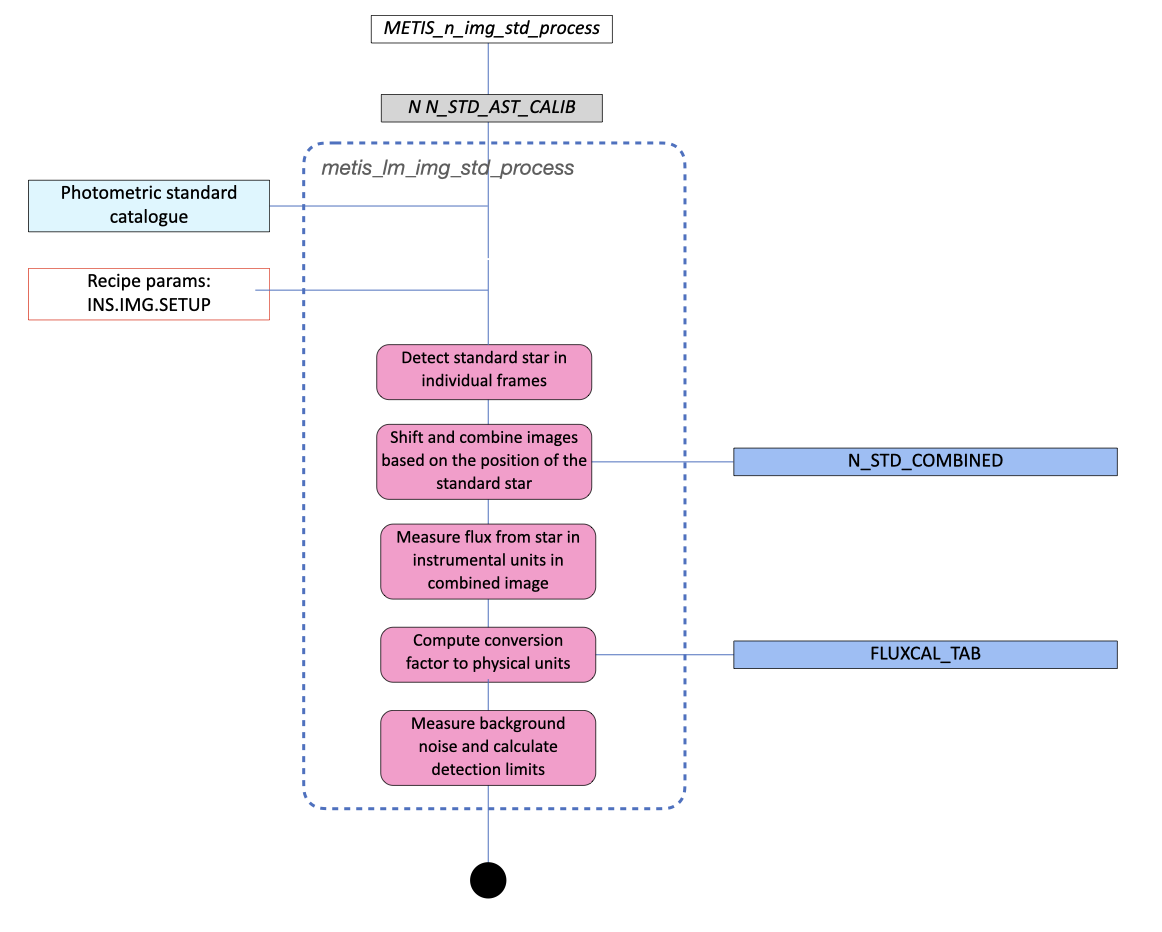
\includegraphics[width=0.6\textwidth]{metis_n_img_std_process}
  %\resizebox{0.6\textwidth}{0.1\textwidth}{\TODO{\fbox{Figure to be done}}}
  \caption[Recipe: \REC{metis_n_img_std_process}]{\REC{metis_n_img_std_process} --
    compute conversion between ADU and physical flux units.}
  \label{fig:metis_n_img_std_process}
\end{figure}


%%%%%%%%%%%%%%%%%%%%%
\clearpage

\subsubsection{N-band imaging calibration}
\label{n_img_calibrate}
\label{rec:n_img_calibrate}
\label{sssec:n_img_calibrate}
\label{rec:metis_n_img_calibrate}

This recipe applies the flux calibration to the chop-nod difference
image. A unique geometric calibration is not possible at this point,
although one could take one of the beams (e.g.\ the positive beam in a
parallel two-point chop-nod pattern) as reference for a
WCS. Distortion information can be added without a reference point as
it pertains to the detector/focal plane, not to the field.

The products of this recipe is the fully calibrated chop-nod
difference image.

The image is multiplied by the conversion factor such that pixel
values are in units of photons per second per centimetre squared. The
header receives the keyword \FITS{BUNIT} with value %
\CODE{'photon.s**(-1).cm**(-2)'}.

\begin{recipedef}
  Name:              & \REC{metis_n_img_calibrate}                      \\
  Purpose:           & Convert science image to physical units          \\
                     & Add distortion information                       \\
  Type:              & Calibration                                      \\
  Templates:         &                                                  \\
  Input data:        & \PROD{N_SCI_BKG_SUBTRACTED}                      \\
                     & \PROD{FLUXCAL_TAB}                               \\
                     & \PROD{N_DISTORTION_TABLE}                        \\
  Matched keywords:  & Filter ID                                        \\
  Parameters:        & TBD                                              \\
  Algorithm:         & call \REC{n_scale_image_flux} to Scale image data to ph/s \\
                     & call \REC{n_add_header_distortion} to add header information (\FITS{BUNIT}, etc.)\\
  Output data:       & \PROD{N_SCI_CALIBRATED}                          \\
  QC1 parameters:    & None                                             \\
\end{recipedef}

\begin{figure}[hb]
  \centering
   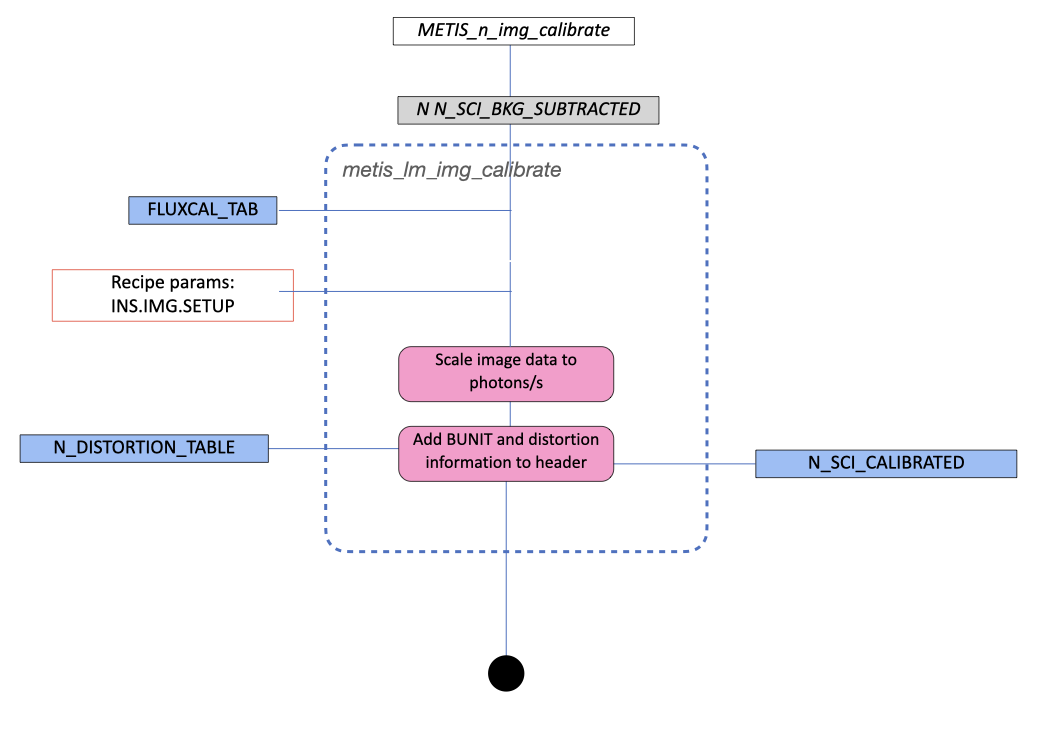
\includegraphics[width=0.6\textwidth]{metis_n_img_calibrate}
  \caption[Recipe: \REC{metis_n_img_calibrate}]{\REC{metis_n_img_calibrate} --
    convert image to physical flux units and update FITS header}
  \label{fig:metis_n_img_calibrate}
\end{figure}

%%%%%%%%%%%%%
\clearpage

\subsubsection{N-band imaging restoration}
\label{n_img_restoration}
\label{rec:n_img_restoration}
\label{sssec:n_img_restoration}

This recipe attempts to combine the positive and negative beams of the
chop-nod difference image into a single positive image of the
source. For compact sources with a size smaller than half the distance
between the beams, it suffices to cut out small regions around the
source images and add the with the appropriate signs to obtain a
single image.

Algorithms for image restoration of extended sources exist but it
remains \TBD\ whether these are sufficiently simple and robust to be
included in the pipeline (cf.\ Sect.~8.8 of \cite{DRLS}).

\begin{recipedef}
  Name:              & \REC{metis_n_img_restore}                                     \\
  Purpose:           & Restore a single positive beam from chop-nod difference image \\
  Type:              & Science                                                       \\
  Input data:        & \CODE{N_SCI_CALIBRATED}                                       \\
  Parameters:        & size of cutout region                                         \\
  Algorithm:         & Cut regions around beams                                      \\
                     & Add regions with appropriate signs                            \\
  Output data:       & \PROD{N_SCI_RESTORED}                                         \\
  QC1 parameters:    & None                                                          \\
  hdrl functions:    & \CODE{hdrl_imagelist_collapse}                                \\
\end{recipedef}

\begin{figure}[hb]
  \centering
  % 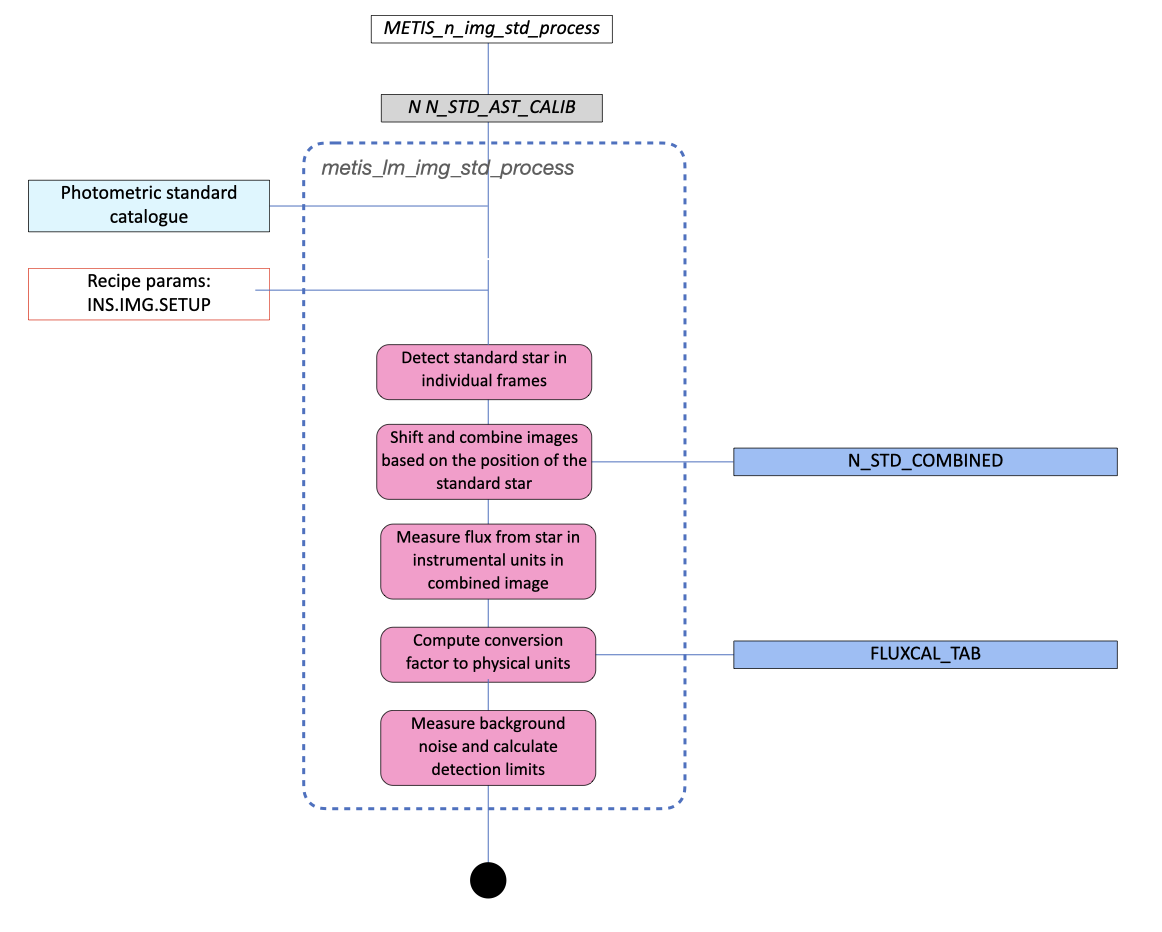
\includegraphics[width=0.6\textwidth]{metis_n_img_std_process}
  \resizebox{0.6\textwidth}{0.1\textwidth}{\TODO{\fbox{Figure to be done}}}
  \caption[Recipe: \REC{metis_n_img_restore}]{\REC{metis_n_img_restore} --
    Create a single positive image from chop-nod difference image}
  \label{fig:metis_n_img_restore}
\end{figure}

%%%%%%%%%%%%%%
\clearpage
\subsubsection{N-band imaging distortion calibration}
\label{n_img_distortion}
\label{rec:n_img_distortion}
\label{sssec:n_img_distortion}

Calibration of the imaging distortion is done on an image of a pin
hole mask located in a focal plane within the instrument. The
distortion is described in terms of a polynomial model whose
coefficients can be transformed to WCS keywords and applied to any
other pipeline product. In addition to the distortion table, a map of
pixel scale across the detector will be created.

\begin{recipedef}
  Name:                & \REC{metis_n_img_distortion}                                   \\
  Purpose:             & Determine optical distortion coefficients for the N imager.    \\
  Templates:           & \TPL{METIS_img_n_cal_distortion}                               \\
  Type:                & Calibration                                                    \\
  Input data:          & Images of grid mask in WCU-FP2 or CFO-FP2.                     \\
                       & Image with WCU window closed (background).                     \\
                       & Grid of pinhole mask positions \\
                       & Bad pixel map                                                  \\
  Parameters:          & Parameters for fitting routine \\
                       & \TBD \\
  Algorithm:           & Subtract background image.  (\CODE{hdrl_imagelist_sub_image})                                       \\
                       & Measure location of point source images in frames.   (\CODE{hdrl_catalogue_create})            \\
                       & call \hyperref[drl:fit_distortion]{\CODE{fit_distortion}} to fit polynomial coefficients to deviations from grid positions. \\
  Output data:         & \hyperref[dataitem:n_distortion_table]{\PROD{N_DISTORTION_TABLE}} \\
                       & \hyperref[dataitem:n_distortion_map]{\PROD{N_DISTORTION_MAP}}        \\
                       & \hyperref[dataitem:n_dist_reduced]{\PROD{N_DIST_REDUCED}}             \\
  Expected accuracies: & TBD                                                            \\
  QC1 parameters:      & \hyperref[qc:qc_n_distort_rms]{\QC{QC N DISTORT RMS} }                                         \\
                       & \hyperref[qc:qc_n_distort_nsource]{\QC{QC LM DISTORT NSOURCE}}  \\
  hdrl functions:      & \CODE{hdrl_catalogue_create}                                   \\
                       & \CODE{hdrl_imagelist_sub_image}                                \\
\end{recipedef}

\begin{figure}[hb]
  \centering
  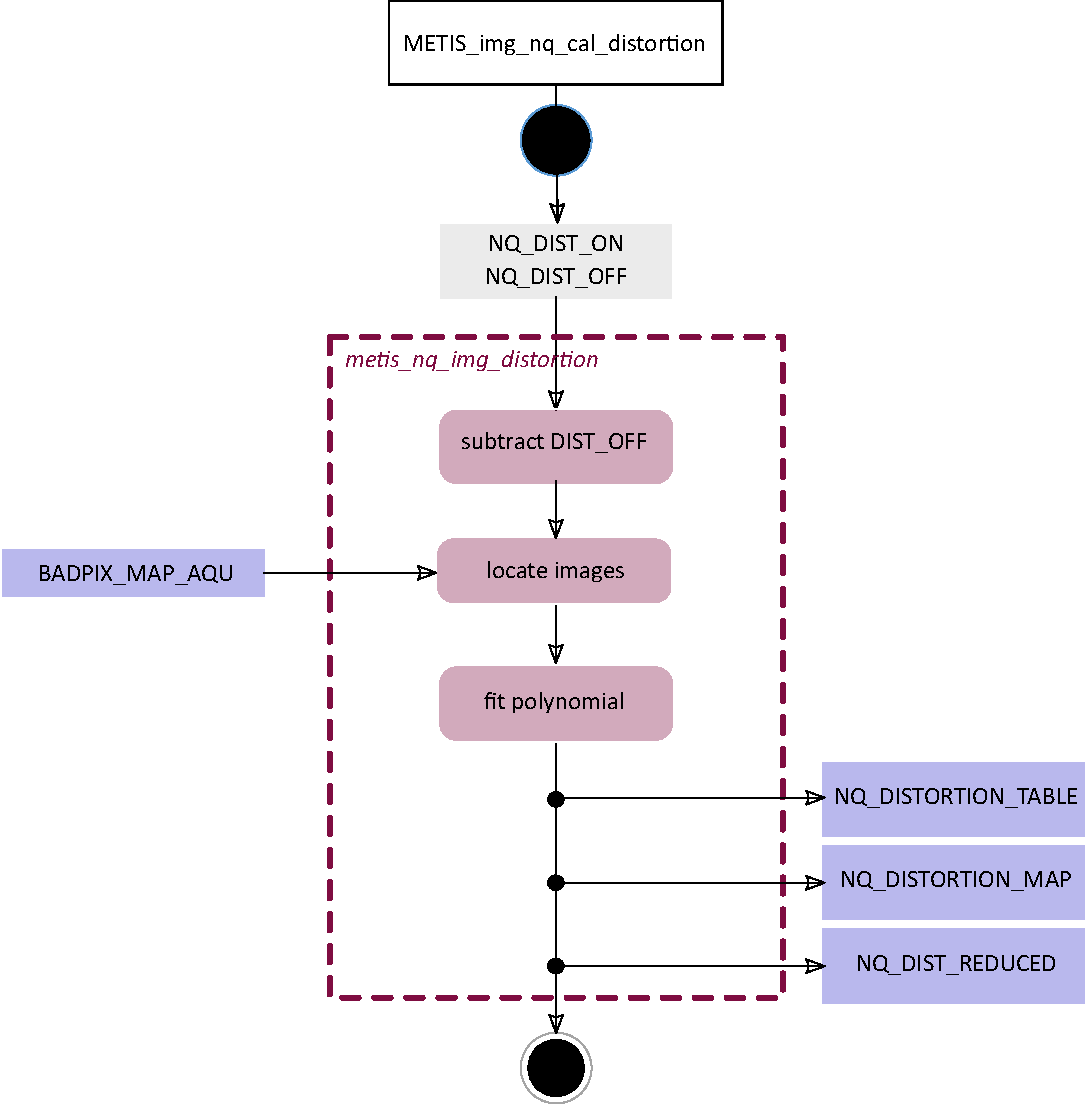
\includegraphics[width=0.6\textwidth]{metis_n_img_distortion}
  \caption[Recipe: \REC{metis_n_img_distortion}]{%
    \REC{metis_n_img_distortion} -- \CODE{IMG_N} distortion calibration}
  \label{fig:metis_n_img_distortion}
\end{figure}

%%% Local Variables:
%%% TeX-master: "METIS_DRLD"
%%% End:

\clearpage
\subsection{Long-slit spectroscopy, LM band}
\label{ssec:recipes_lss_lm}

A draft of the reduction cascade is shown in
Figs.~\ref{Fig:LMLssAssomap1} and \ref{Fig:LMLssAssomap2} together with the data processing table
(Tables~\ref{Tab:LMLssDatProc1} and ~\ref{Tab:LMLssDatProc2}). The first part aims to update the static calibration database, in particular the creation of the gain map (\hyperref[Sec:detector_calibration]{\REC{metis_det_lingain}}) and the determination of the \ac{ADC} slitlosses (\hyperref[rec:metis_lm_adc_slitloss]{\REC{metis_lm_adc_slitloss}}). These are executed only when an update is required, e.g. after a major instrument interention or on yearly basis. The second part comprises the basic calibrations, e.g. the dark correction and the spectroscopic flatfielding via \ac{RSRF}, followed by the third part, the main calibration steps, incorporating the determination of the first guess wavelength solution by means of the laser sources in the \ac{WCU} and the determination of the response curve for the flux calibration. Subsequently, the main reduction is conducted, which applies the previously created master calibration files to the science frames. Both, the flux standard and the science observations are wavelength calibrated with the help of the atmospheric lines visible in the respective spectra. Therefore the main step of the wavelength calibration is carried out in the recipes \hyperref[rec:metis_lm_lss_std]{\REC{metis_LM_lss_std}} and \hyperref[rec:metis_lm_lss_sci]{\REC{metis_LM_lss_sci}}. Finally, the telluric absorption correction is applied using the modelling approach with \texttt{molecfit}. Optionally, the telluric correction can be done with a telluric standard star.


%------------------------------------------------------------------------------------------------------------------
\subsubsection{Recipes \REC{metis_det_lingain} and \REC{metis_det_dark}}
These recipes are described in Section~\ref{Sec:detector_calibration}.

%------------------------------------------------------------------------------------------------------------------
\subsubsection{Recipe \REC{metis_LM_adc_slitloss}}
The recipe \hyperref[sssec:adc_slitlosses]{\REC{metis_LM_adc_slitloss}} aims to determine the slit losses induced by the fixed \ac{ADC} positions as function of the object position across the slit. The recipe aims to create a table with slitlosses (\hyperref[dataitem:lm_adc_slitloss]{\STATCALIB{LM_ADC_SLITLOSS}}), which is added to the static database and used in the recipes \hyperref[rec:metis_lm_lss_std]{\REC{metis_LM_lss_std}}. This recipe is to be carried out only when an update of the database is needed. The algorithm and the workflow of the recipe to determine the slitlosses is given in Section~\ref{sssec:adc_slitlosses}, more information can be found in Section "Calibration of slit losses" in the Calibration Plan \cite{METIS-calibration_plan}. 


%------------------------------------------------------------------------------------------------------------------
\subsubsection{LM-LSS Flatfielding recipe \REC{metis_LM_lss_rsrf}:}\label{rec:metis_lm_lss_rsrf}
The recipe \hyperref[rec:metis_lm_lss_rsrf]{\REC{metis_LM_lss_rsrf}} aims to create a spectroscopic master flatfield for determining the pixel-to-pixel sensitivity and to enable the order location algorithm (\hyperref[rec:metis_lm_lss_trace]{\REC{metis_LM_lss_trace}}).
\begin{figure}[ht]
  \centering
  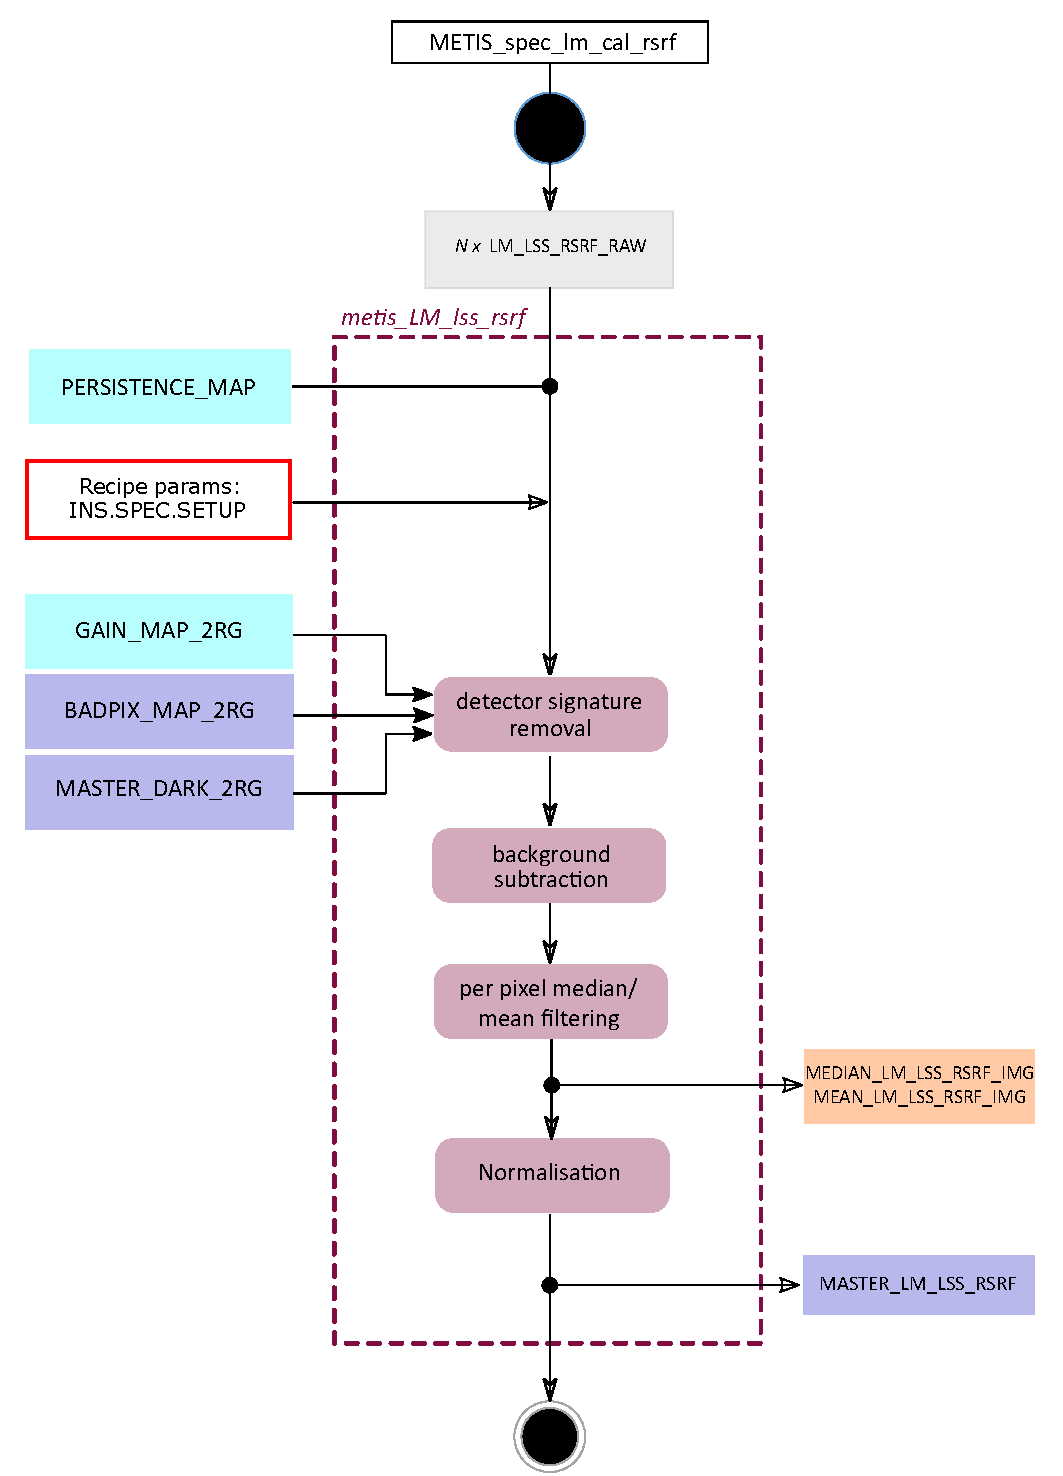
\includegraphics[width=0.5\textheight]{figures/metis_lm_lss_rsrf_v0.82.pdf}
  \caption[Recipe: \REC{metis_LM_lss_rsrf}]{\REC{metis_LM_lss_rsrf} --
    Recipe workflow to create the spectroscopic flatfield by means of the \ac{RSRF}.}
  \label{Fig:rec_lm_lss_rsrf}
\end{figure}

\begin{recipedef}
Name:		& \hyperref[rec:metis_lm_lss_rsrf]{\REC{metis_LM_lss_rsrf}}  \\
Purpose:	& Spectroscopic flatfielding with \ac{RSRF} \\
Type:		& Calibration\\
Requirements: & None \\
Templates:           & \TPL{METIS_spec_lm_cal_rsrf} \\
Input data:     & $N\times$ \hyperref[dataitem:lm_lss_rsrf_raw]{\RAW{LM_LSS_RSRF_RAW}} \\
                & \hyperref[dataitem:persistence_map]{\EXTCALIB{PERSISTENCE_MAP}}  \\
                & \hyperref[dataitem:gain_map_lm]{\STATCALIB{GAIN_MAP_LM}}  \\
                & \hyperref[dataitem:badpix_map_lm]{\PROD{BADPIX_MAP_LM}}  \\
                & \hyperref[dataitem:master_dark_lm]{\PROD{MASTER_DARK_LM}}  \\
Parameters: 	& TBD\\
Algorithm:      & subtract master \ac{WCU} "OFF" frame from illumination frame (done on individual images)\\
                & median/mean filtering of subtracted images\\
                & division by blackbody spectrum\\
                & normalisation to achieve \ac{RSRF}\\
Output data:	& \hyperref[dataitem:master_lm_lss_rsrf]{\PROD{MASTER_LM_LSS_RSRF}} (\FITS{PRO.CATG=MASTER_LM_LSS_RSRF}): \\
                & \hyperref[dataitem:median_lm_lss_rsrf_img]{\PROD{MEDIAN_LM_LSS_RSRF_IMG}}\\
                & \hyperref[dataitem:mean_lm_lss_rsrf_img]{\PROD{MEAN_LM_LSS_RSRF_IMG}}\\
Expected accuracies: & 3\% (cf. \cite{METIS-calibration_plan} and \cite{METIS_calerrbudget})\\
QC1 parameters: & \hyperref[qc:lmlssrsrfmeanlevel]{\QC{QC LM LSS RSRF MEAN LEVEL}}: Mean level of the \ac{RSRF}\\
                & \hyperref[qc:lmlssrsrfmedianlevel]{\QC{QC LM LSS RSRF MEDIAN LEVEL}}: Median level of the \ac{RSRF}\\
                & \hyperref[qc:lmlssrsrfintordrlevel]{\QC{QC LM LSS RSRF INTORDR LEVEL}}: Flux level of the interorder background\\
                & \hyperref[qc:lmlssrsrfnormstdev]{\QC{QC LM LSS RSRF NORM STDEV}}: Standard deviation of the normalised \ac{RSRF}\\
                & \hyperref[qc:lmlssrsrfnormsnr]{\QC{QC LM LSS RSRF NORM SNR}}: \ac{SNR} of the normalised \ac{RSRF}\\
                & more TBD\\
\end{recipedef}
\clearpage

%------------------------------------------------------------------------------------------------------------------
\subsubsection{LM-LSS Order detection \REC{metis_LM_lss_trace}:}\label{rec:metis_lm_lss_trace}
The recipe \hyperref[rec:metis_lm_lss_trace]{\REC{metis_LM_lss_trace}} aims at detecting the orders and a polynomial fitting of the order locations (see \cite{pis02} and \cite{pis21} for details on the algorithms). The detection and polynomial fitting is based on flatfield frames taken through a pinhole mask, which leads to individual pinhole traces along the entire dispersion direction.

\begin{figure}[ht]
  \centering
  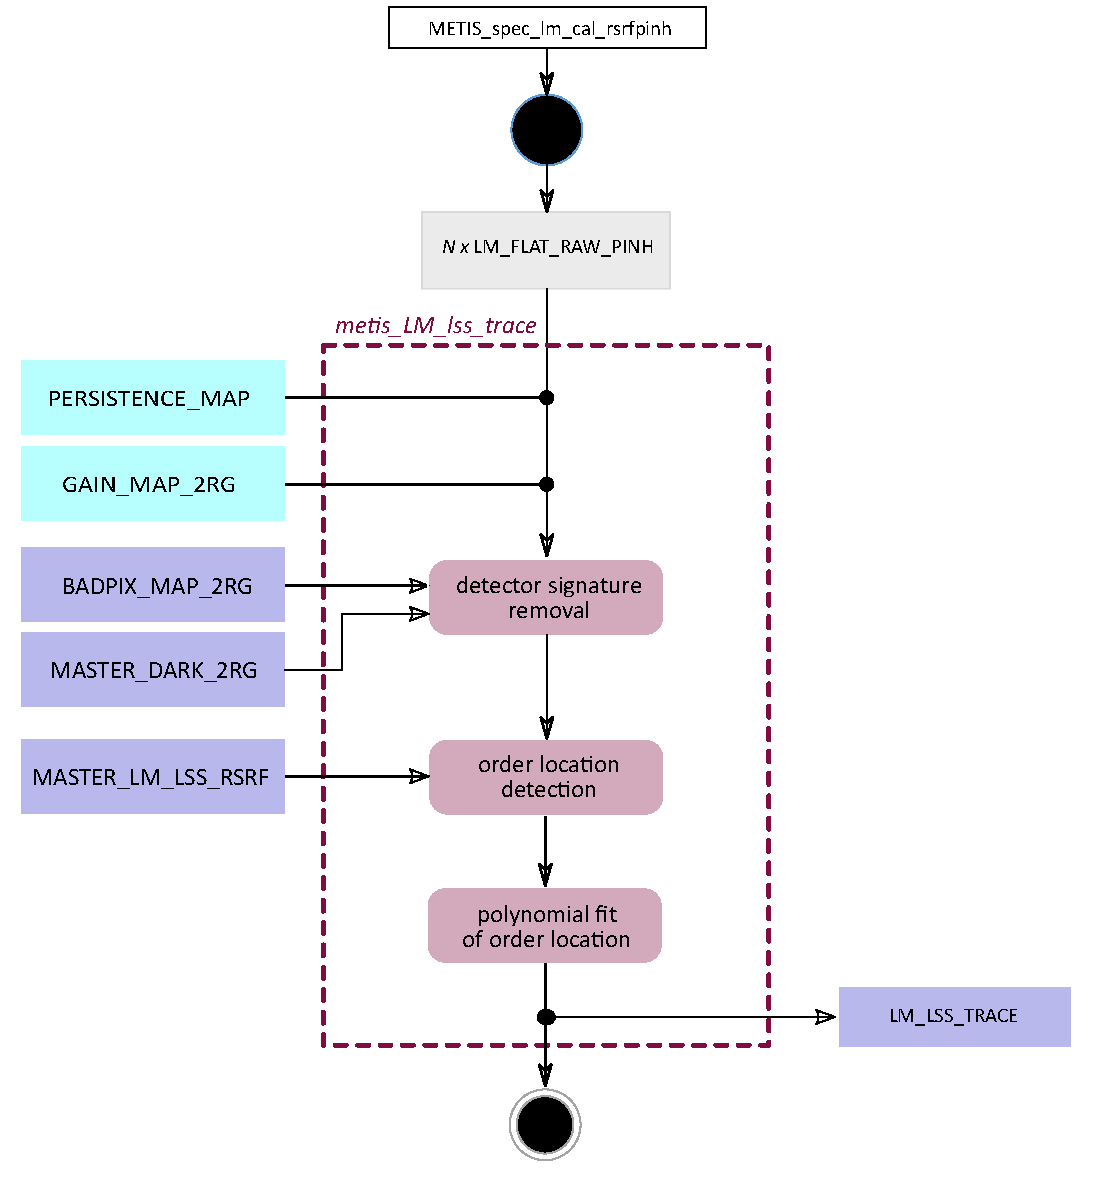
\includegraphics[width=0.5\textheight]{figures/metis_lm_lss_trace_v0.82.pdf}
  \caption[Recipe: \REC{metis_LM_lss_trace}]{\REC{metis_LM_lss_trace} --
    Detection and polynomial fitting of the order location.}
  \label{Fig:rec_lm_lss_wtrace}
\end{figure}

\begin{recipedef}
Name:		&  \hyperref[rec:metis_lm_lss_trace]{\REC{metis_LM_lss_trace}} \\
Purpose:	& Detection of order location \\
Type:		& Calibration\\
Requirements: & None \\
Templates:           & \TPL{METIS_spec_lm_cal_InternalWave}  \\
Input data:     & $N\times$ \hyperref[dataitem:lm_lss_rsrf_pinh_raw]{\RAW{LM_LSS_RSRF_PINH_RAW}} \\
                & \hyperref[dataitem:persistence_map]{\EXTCALIB{PERSISTENCE_MAP}}  \\
                & \hyperref[dataitem:gain_map_lm]{\STATCALIB{GAIN_MAP_LM}}  \\
                & \hyperref[dataitem:badpix_map_lm]{\PROD{BADPIX_MAP_LM}}  \\
                & \hyperref[dataitem:master_dark_lm]{\PROD{MASTER_DARK_LM}}  \\
                & \hyperref[dataitem:master_lm_lss_rsrf]{\PROD{MASTER_LM_LSS_RSRF}} \\
Parameters: 	& polynomial degree\\
Algorithm:      & Detection of the order edges\\
                & Polynomial fitting\\
Output data:	& \hyperref[dataitem:lm_lss_trace]{\PROD{LM_LSS_TRACE}} (\FITS{PRO.CATG=LM_LSS_TRACE}): Polynomial coefficients\\
Expected accuracies: & (TBD)\\
QC1 parameters: & \hyperref[qc:lmlsstracelpolydeg]{\QC{QC LM LSS TRACE LPOLYDEG}}: Degree of the polynomial fit of the left order edge\\
                & \hyperref[qc:lmlsstracelcoeffi]{\QC{QC LM LSS TRACE LCOEFF<i>}}: $i$-th coefficient of the polynomial of the left order edge\\
                & \hyperref[qc:lmlsstracerpolydeg]{\QC{QC LM LSS TRACE RPOLYDEG}}: Degree of the polynomial fit of the right order edge\\
                & \hyperref[qc:lmlsstracercoeffi]{\QC{QC LM LSS TRACE RCOEFF<i>}}: $i$-th coefficient of the polynomial of the right order edge\\
                & \hyperref[qc:lmlsstraceintrordrlevel]{\QC{QC LM LSS TRACE INTORDR LEVEL}}: Flux level of the interorder background\\
                & more TBD\\
\end{recipedef}

\clearpage
%------------------------------------------------------------------------------------------------------------------
\subsubsection{LM-LSS wavelength calibration recipe \REC{metis_LM_lss_wave}:}\label{rec:metis_lm_lss_wave}
This recipe aims at determining the first guess of the wavelength calibration on basis of the \ac{WCU} laser sources (c.f. \cite{METIS-calibration_plan}). Therefore the first steps are the removal of the detector signature of the \FITS{LM_WAVE_RAW} frames by applying the master calibration files derived in the previous steps, following by the background subtraction (if needed, TBD) and the application of the RSRF. The distortion of the lines (i.e. possible tilt, curvature,...) and the wavelength solution is determined by the algorithm developed by Piskunov et al. (\cite{pis02}, \cite{pis21}). The reference frame is defined by the laser line catalogue (\hyperref[dataitem:laser_tab]{\STATCALIB{LASER_TAB}}).

 This is in compliance with \REQ{METIS-6074}.

\begin{figure}[ht]
  \centering
  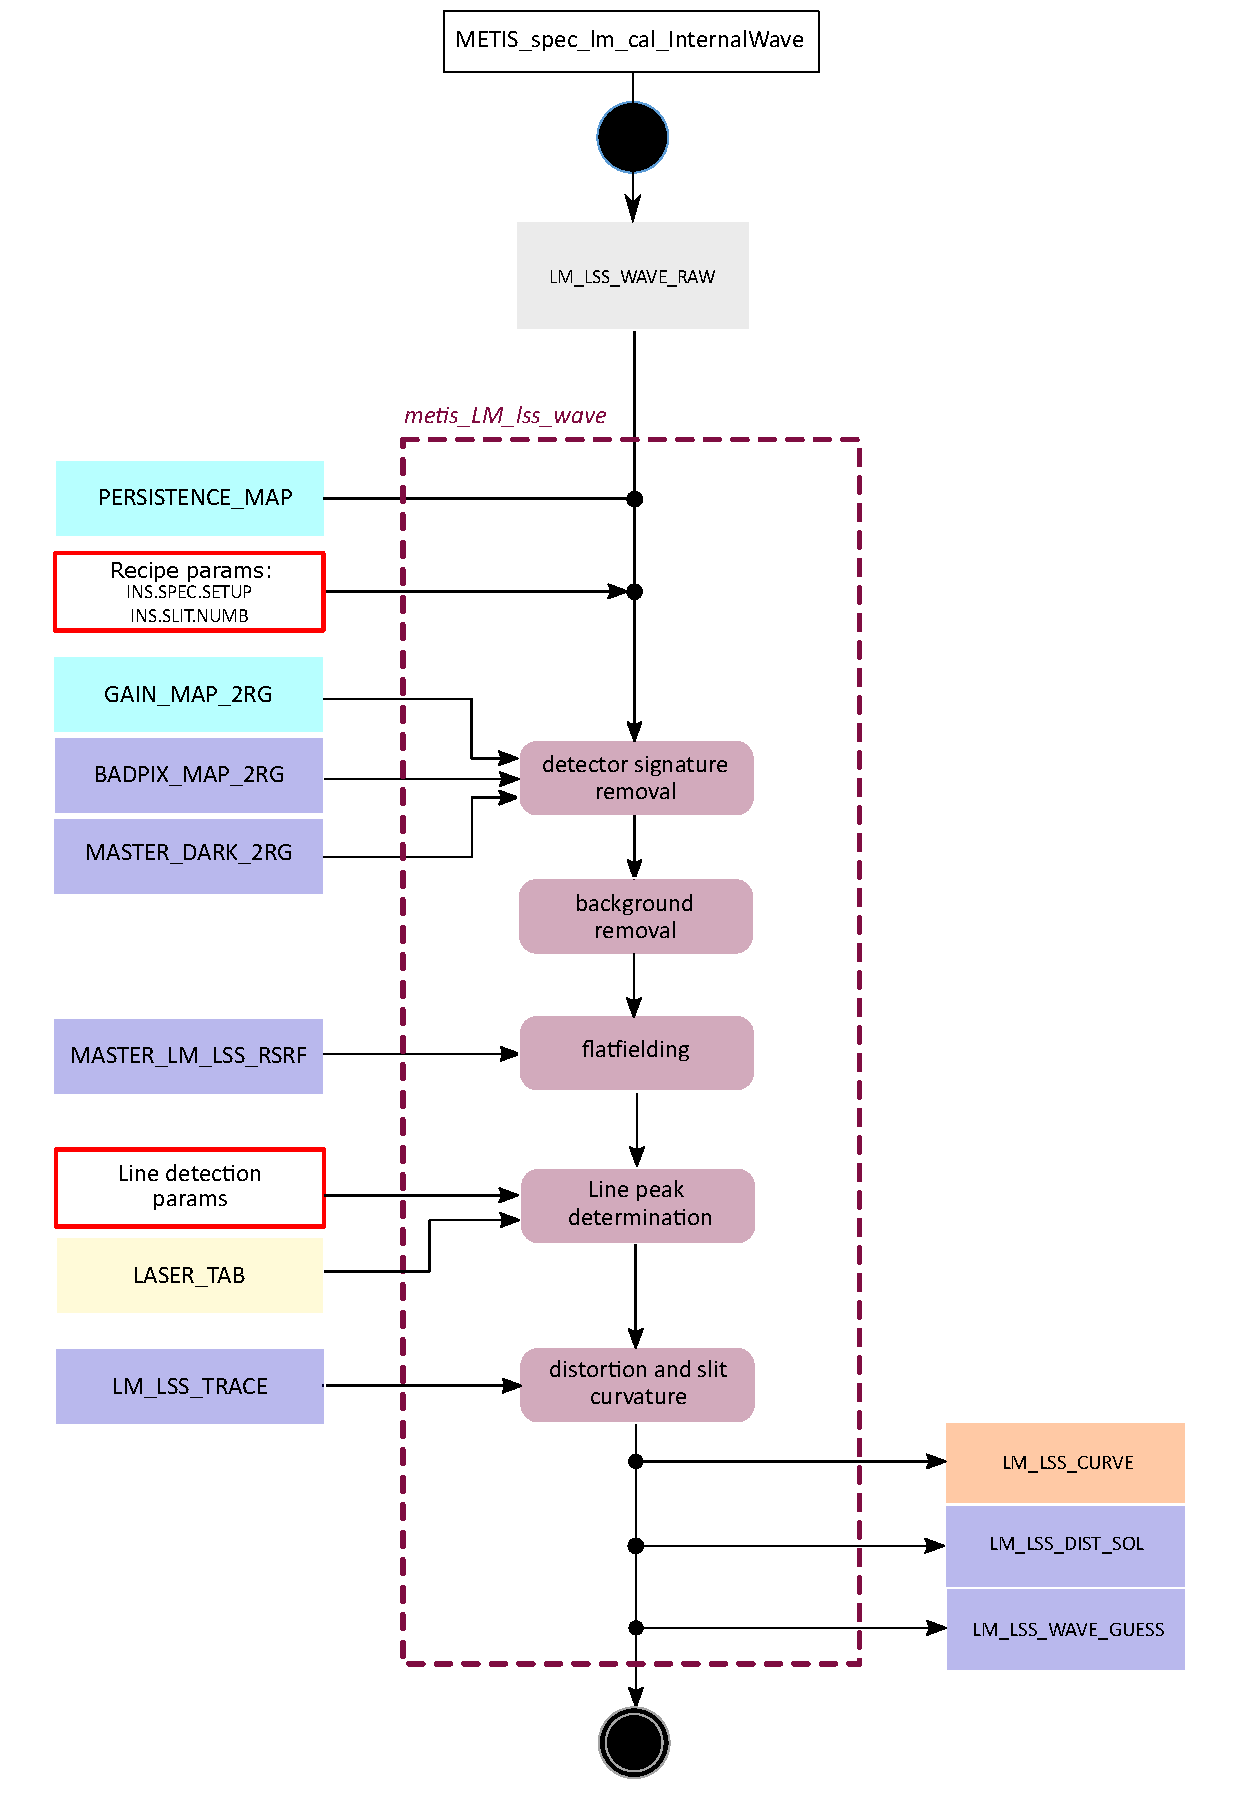
\includegraphics[width=0.5\textheight]{figures/metis_lm_lss_wave_v0.82.pdf}
  \caption[Recipe: \REC{metis_LM_lss_wave}]{\REC{metis_LM_lss_wave} --
    Creation of the LM LSS master wavelength correction.}
  \label{Fig:rec_lm_lss_trace}
\end{figure}
\clearpage

\begin{recipedef}
Name:		& \hyperref[rec:metis_lm_lss_wave]{\REC{metis_LM_lss_wave}} \\
Purpose:	& Wavelength calibration \\
Type:		& Calibration\\
Requirements: & METIS-6084, METIS-1371, METIS-6074 \\
Templates:           & \TPL{METIS_spec_lm_cal_internalwave}, \\
Input data: 	& \hyperref[dataitem:lm_lss_wave_raw]{\RAW{LM_LSS_WAVE_RAW}}\\
                & \hyperref[dataitem:persistence_map]{\EXTCALIB{PERSISTENCE_MAP}}  \\
                & \hyperref[dataitem:gain_map_lm]{\STATCALIB{GAIN_MAP_LM}}  \\
                & \hyperref[dataitem:badpix_map_lm]{\PROD{BADPIX_MAP_LM}}  \\
                & \hyperref[dataitem:master_dark_lm]{\PROD{MASTER_DARK_LM}}  \\
                & \hyperref[dataitem:master_lm_lss_rsrf]{\PROD{MASTER_LM_LSS_RSRF}} \\
                & \hyperref[dataitem:lm_lss_trace]{\PROD{LM_LSS_TRACE}} \\
                & \hyperref[dataitem:laser_tab]{\STATCALIB{LASER_TAB}} \\
                % & \hyperref[dataitem:ref_airg_cat]{\STATCALIB{REF_AIRG_CAT}} \\
Parameters: 	& (TBD)\\
Algorithm:      & Application of detector master calibration files\\
                & Determination and application of the distortion correction\\
                & Determination of the first guess of the wavelength solution by polynomial fit of the detected laser source lines\\
Output data:	& \hyperref[dataitem:lm_lss_curve]{\PROD{LM_LSS_CURVE}} (\FITS{PRO.CATG=LM_LSS_CURVE}): Curvature \\
                & \hyperref[dataitem:lm_lss_dist_sol]{\PROD{LM_LSS_DIST_SOL}} (\FITS{PRO.CATG=LM_LSS_DIST_SOL}): Distortion solution\\
                & \hyperref[dataitem:lm_lss_wave_guess]{\PROD{LM_LSS_WAVE_GUESS}} (\FITS{PRO.CATG=LM_LSS_WAVE_GUESS}): Wavelength first guess\\
Expected accuracies: & 1/5th of a pixel after post-processing (cf. \cite{METIS-calibration_plan})\\
QC1 parameters: & \hyperref[qc:lmlsswavepolydeg]{\QC{QC LM LSS WAVE POLYDEG}}: Degree of the first guess polynomial\\
                & \hyperref[qc:lmlsswavecoeffi]{\QC{QC LM LSS WAVE COEFF<i>}}: $i$-th coefficient of the polynomial\\
                & \hyperref[qc:lmlsswavenlines]{\QC{QC LM LSS WAVE NLINES}}: Number of detected (laser) lines; should be constant\\
                & \hyperref[qc:lmlsswavelinefwhmavg]{\QC{QC LM LSS WAVE LINEFWHMAVG}}: Average of the \ac{FWHM} of the detected lines (should be widely constant)\\
                & \hyperref[qc:lmlsswaveinterordrlevel]{\QC{QC LM LSS WAVE INTORDR LEVEL}}: Flux level of the interorder background\\
                & more TBD: e.g. QC params for distortion determination and correction\\
\end{recipedef}

\clearpage
%------------------------------------------------------------------------------------------------------------------
\subsubsection{LM-LSS standard star calibration recipe \REC{metis_LM_lss_std}:}\label{rec:metis_lm_lss_std}
\TODO{Finish following text} 

This recipe aims at processing standard stars used for the absolute flux calibration and (optionally) for the telluric feature removal: As first step the detector master calibration files derived previously are applied followed by the background subtraction, if needed the distortion correction (\hyperref[dataitem:lm_lss_dist_sol]{\PROD{LM_LSS_DIST_SOL}}), and
the wavelength calibration by means of the first guess solution (\hyperref[dataitem:lm_lss_wave_guess]{\PROD{LM_LSS_WAVE_GUESS}}) and the telluric sky lines (c.f. Sect.\,8.5 in \cite{DRLS}). Then the recipe removes sky background, extracts the standard star spectrum object and collapses the 2D to 1D spectra. To better compare the corresponding model spectrum a telluric correction is required. This is done by means of the standard star observations itself or (optionally) with \texttt{molecfit}.\\
It is on the user's decision whether the standard star is used for the absolute flux calibration only, or also used for the telluric correction of the science target.

As one needs to determine the stellar continuum regions, a telluric correction is required to increase these regions. This can be done either by applying a fairly simple telluric correction in an automated way to the standard star spectrum. In case the the user decides to use the standard star also for the telluric correction, a transmission function is derived from that in the "classical" way (cf. Section~\ref{sssec:tecllcorrclassic}), which will be optionally used for the telluric correction also for the science target. This star spectrum can also be optionally used for the wavelength solution and for the flux calibration, if the \ac{TSS} is suited for that. The response curve is obtained by comparing the extracted spectrum with a model and/or another reference spectrum of the standard star. Currently it is foreseen to use the same standard stars as in \ac{CRIRES}/CRIRES+ and \ac{VISIR}. It is under investigation whether more stars are needed.
\begin{figure}[ht]
  \centering
  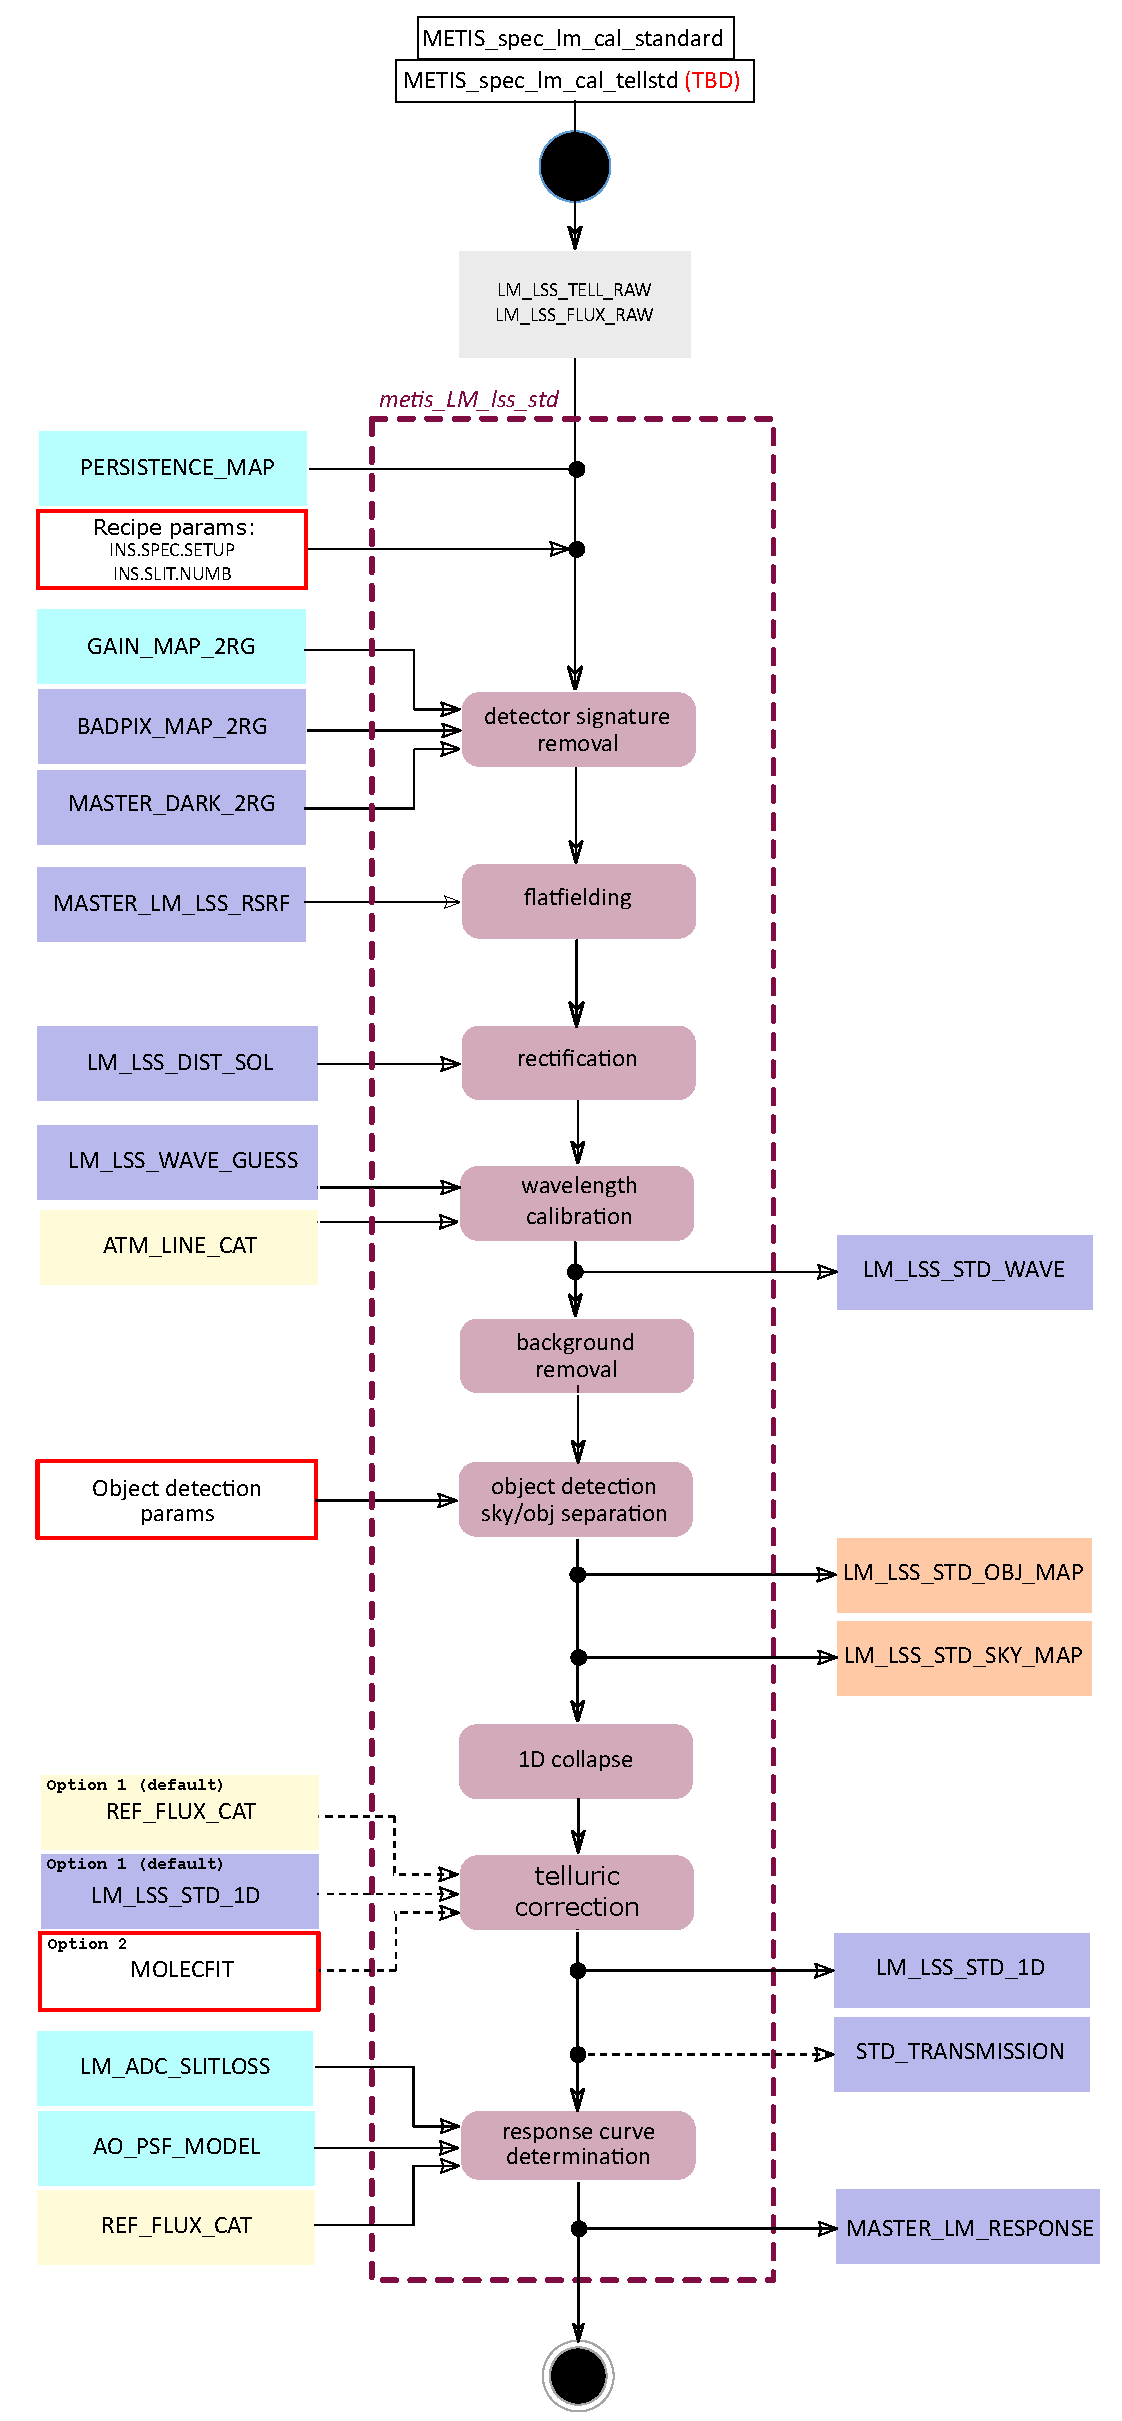
\includegraphics[width=0.4\textheight]{figures/metis_lm_lss_std_v0.82.pdf}
  \caption[Recipe: \REC{metis_LM_lss_std}]{\REC{metis_LM_lss_std} --
    Calibration recipe for processing standard stars for (combined) telluric and  spectro-photometric calibration.}
  \label{Fig:rec_lm_lss_flux1}
\end{figure}
%\begin{figure}[ht]
%  \centering
%  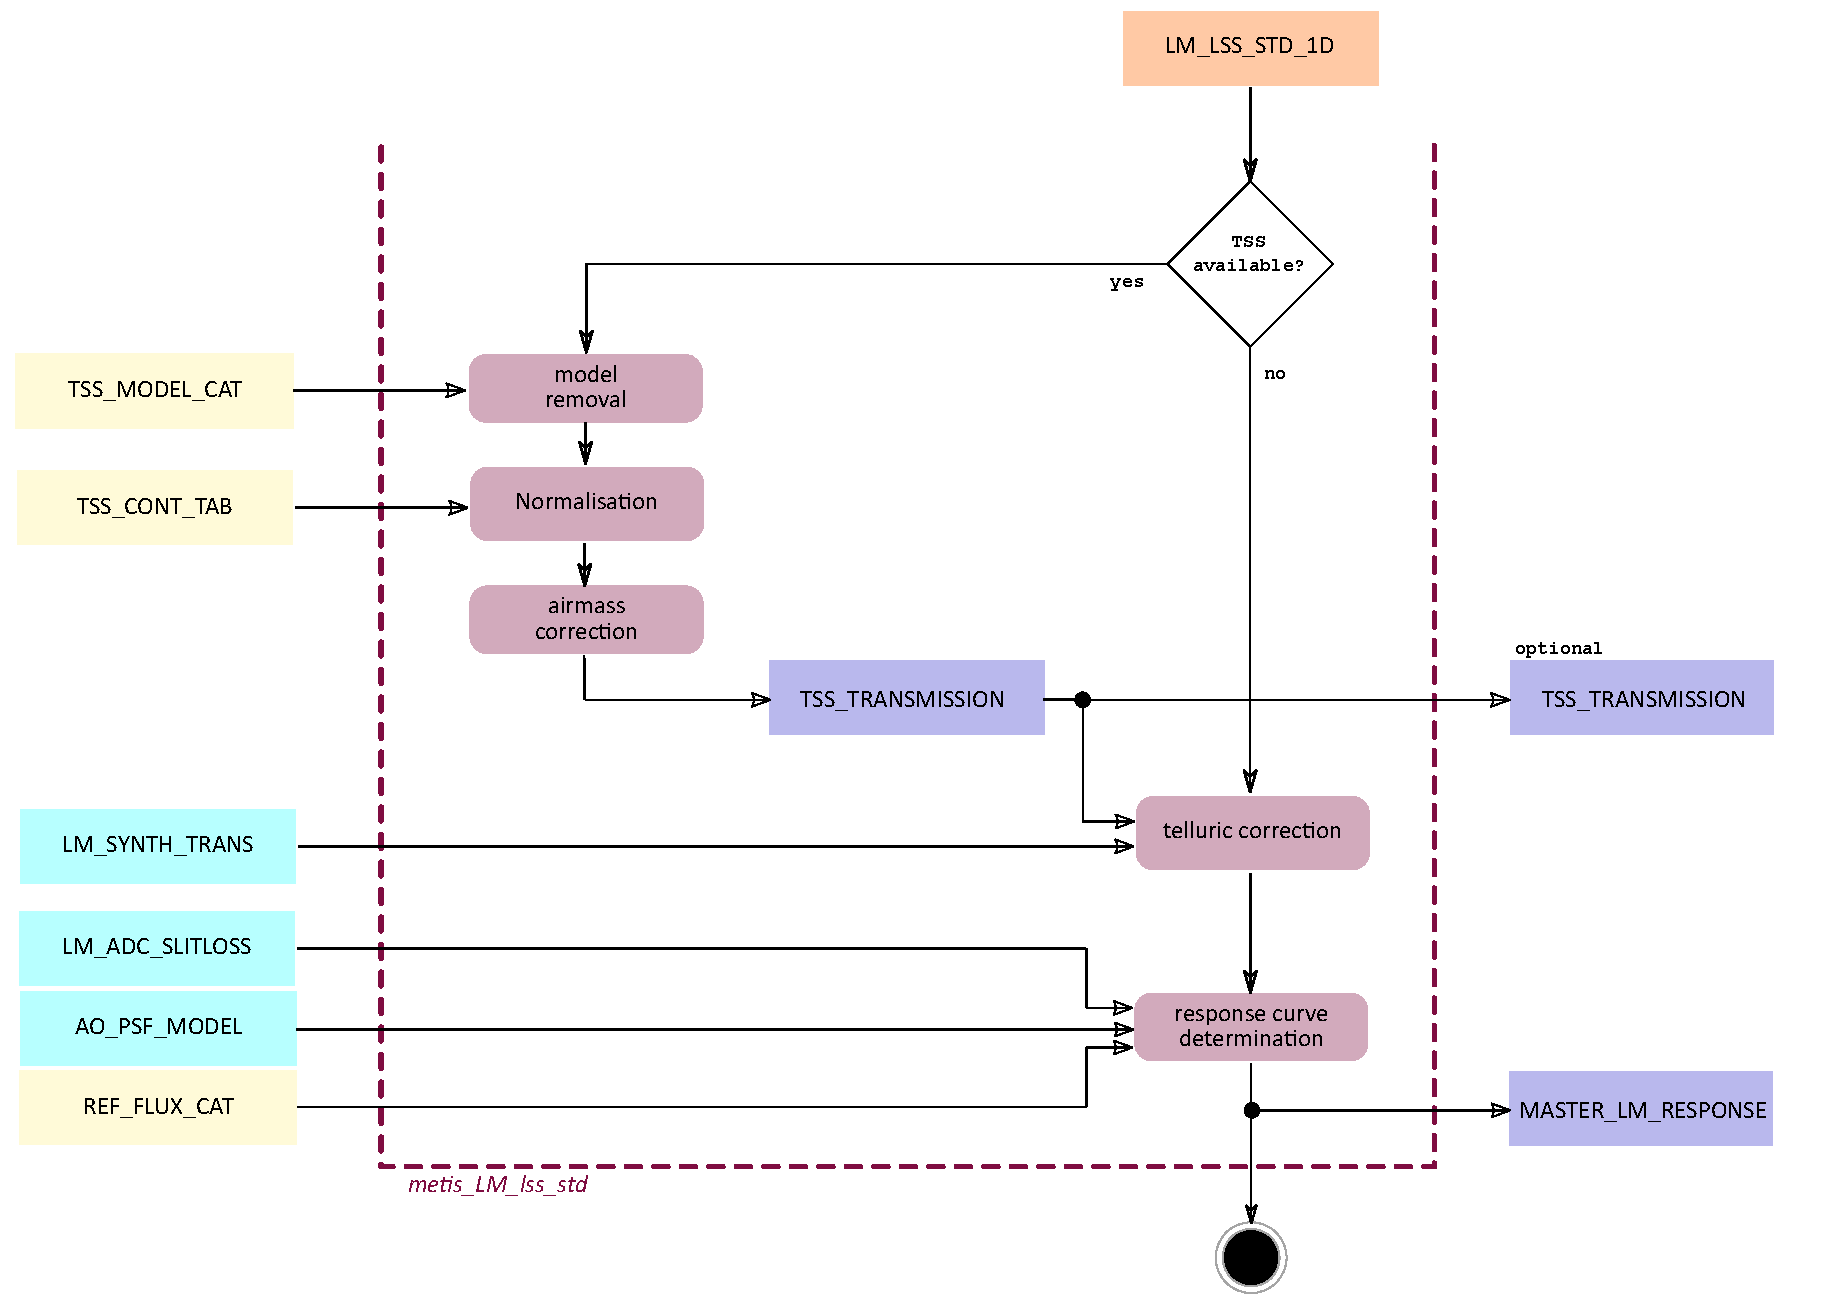
\includegraphics[width=0.6\textheight]{figures/metis_lm_lss_std_v0.8_part_2.pdf}
%  \caption[Recipe: \REC{metis_LM_lss_std}]{\REC{metis_LM_lss_std} --
%    Part 2 of the calibration recipe for processing spectrophotometric and telluric standard stars.}
%  \label{Fig:rec_lm_lss_flux2}
%\end{figure}
\clearpage
\begin{recipedef}
Name:		& \hyperref[rec:metis_lm_lss_std]{\REC{metis_LM_lss_std}} \\
Purpose:	& Flux calibration \\
Type:		& Calibration\\
Requirements: & METIS-6084, METIS-6074 \\
Templates:           & \TPL{METIS_spec_lm_cal_standard}\\
Input data: 	& \hyperref[dataitem:lm_lss_flux_raw]{\RAW{LM_LSS_FLUX_RAW}}\\
                & \hyperref[dataitem:persistence_map]{\EXTCALIB{PERSISTENCE_MAP}}  \\
                & \hyperref[dataitem:gain_map_lm]{\STATCALIB{GAIN_MAP_LM}}  \\
                & \hyperref[dataitem:badpix_map_lm]{\PROD{BADPIX_MAP_LM}}  \\
                & \hyperref[dataitem:master_dark_lm]{\PROD{MASTER_DARK_LM}}  \\
                & \hyperref[dataitem:master_lm_lss_rsrf]{\PROD{MASTER_LM_LSS_RSRF}} \\
                & \hyperref[dataitem:lm_lss_dist_sol]{\PROD{LM_LSS_DIST_SOL}} \\
                & \hyperref[dataitem:lm_lss_wave_guess]{\PROD{LM_LSS_WAVE_GUESS}} \\
                & \hyperref[dataitem:ao_psf_model]{\EXTCALIB{AO_PSF_MODEL}} \\
                & \hyperref[dataitem:atm_line_cat]{\EXTCALIB{ATM_LINE_CAT}} \\
%                & \hyperref[dataitem:tss_model_cat]{\STATCALIB{TSS_MODEL_CAT}}\\
%                & \hyperref[dataitem:tss_cont_tab]{\STATCALIB{TSS_CONT_TAB}}\\
                & \hyperref[dataitem:lm_adc_slitloss]{\STATCALIB{LM_ADC_SLITLOSS}}\\
                & \hyperref[dataitem:lm_synth_trans]{\STATCALIB{LM_SYNTH_TRANS}}\\
                & \hyperref[dataitem:ref_std_cat]{\STATCALIB{REF_STD_CAT}} \\
Parameters: 	& (TBD)\\
Algorithm:      & Application of master calibration files\\
                & Background removal\\
                & Determination and application of the distortion correction\\
                & Determination and application of the wavelength solution\\
                & Identifying/separatiing sky/object pixels\\
                & Removing sky lines: Creation and Subtraction of 2D sky\\
                & Collapsing 2D to 1D spectrum, (see Fig.\,\ref{Fig:rec_lm_lss_sci})\\
                & Determination and application of response curve\\
Output data:	& \hyperref[dataitem:lm_lss_std_obj_map]{\PROD{LM_LSS_STD_OBJ_MAP}}: Pixel map of object pixels\\
            	& \hyperref[dataitem:lm_lss_std_sky_map]{\PROD{LM_LSS_STD_SKY_MAP}}: Pixel map of sky pixels\\
              	& \hyperref[dataitem:lm_lss_std_1d]{\PROD{LM_LSS_STD_1D}}: coadded, wavelength calibrated, collapsed 1D spectrum\\
              	& \hyperref[dataitem:lm_lss_std_wave]{\PROD{LM_LSS_STD_WAVE}}: Wavelength solution derived from the \ac{STD} star (optional)\\
            	& \hyperref[dataitem:std_transmission]{\PROD{STD_TRANSMISSION}}: Transmission function derived by means of the \ac{STD} (optional)\\        
                & \hyperref[dataitem:master_lm_response]{\PROD{MASTER_LM_RESPONSE}}: response function \\
Expected accuracies: & 10\% over an atmospheric band (ESO Req. R-MET-107)\\
            & $<30$\% absolute line flux accuracy (R-MET-107)\\
            & $<5$\% absolute flux calibration (R-MET-82)\\
QC1 parameters: & \hyperref[qc:lmlssstdbackgdmean]{\QC{QC LM LSS STD BACKGD MEAN}}: Mean value of background\\
                & \hyperref[qc:lmlssstdbackgdmedian]{\QC{QC LM LSS STD BACKGD MEDIAN}}: Median value of background\\
                & \hyperref[qc:lmlssstdbackgdstdev]{\QC{QC LM LSS STD BACKGD STDEV}}: Standard deviation value of background\\
                & \hyperref[qc:lmlssstdsnr]{\QC{QC LM LSS STD SNR}}: Signal-to-noise ration of flux standard star spectrum\\
                & \hyperref[qc:lmlssstdsnrnoise]{\QC{QC LM LSS STD SNRNOISE}}: Noise level of flux standard star spectrum\\
                & \hyperref[qc:lmlssstdfwhm]{\QC{QC LM LSS STD FWHM}}: FWHM of flux standard spectrum\\
                & \hyperref[qc:lmlssfluxintrordravglevel]{\QC{QC LM LSS FLUX INTORDR LEVEL}}: Flux level of the interorder background\\
                & \hyperref[qc:lmlssfluxlevel]{\QC{QC LM LSS FLUX AVGLEVEL}}: Average level of the standard star flux \\
                & \hyperref[qc:lmlssfluxwavecaldevmean]{\QC{QC LM LSS FLUX WAVECAL DEVMEAN}}: Mean deviation from the
                  wavelength reference frame (TBDef)\\
                & \hyperref[qc:lmlssfluxwavecalfwhm]{\QC{QC LM LSS FLUX WAVECAL FWHM}}: Measured FWHM of lines\\
                & \hyperref[qc:lmlssfluxwavecalnident]{\QC{QC LM LSS FLUX WAVECAL NIDENT}}: Number of identified lines\\
                & \hyperref[qc:lmlssfluxwavecalnmatch]{\QC{QC LM LSS FLUX WAVECAL NMATCH}}: Number of lines matched between
                    catalogue and spectrum\\
                & \hyperref[qc:lmlssfluxwavecalpolydeg]{\QC{QC LM LSS FLUX WAVECAL POLYDEG}}: Degree of the polynomial\\
                & \hyperref[qc:lmlssfluxwavecalpolycoeffn]{\QC{QC LM LSS FLUX WAVECAL POLYCOEFF\<n\>}}: $n$-th coefficient of the polynomial\\
                & \hyperref[qc:lmlssfluxstdsnr]{\QC{QC LM LSS FLUX STDSNR}}: Signal-to-noise ration of flux standard star spectrum\\
                & \hyperref[qc:lmlssfluxsnrnoise]{\QC{QC LM LSS FLUX SNRNOISE}}: Noise level of flux standard star spectrum\\
                & \hyperref[qc:lmlssfluxfwhm]{\QC{QC LM LSS FLUX FWHM}}: FWHM of flux standard spectrum\\
                & \hyperref[qc:lmlssfluxpsfloss]{\QC{QC LM LSS FLUX PSFLOSS}}: Fraction of AO induced slit losses (TBdef)\\
                & more TBD
\end{recipedef}

\subsubsection{LM-LSS science reduction recipe \REC{metis_LM_lss_sci}:}\label{rec:metis_lm_lss_sci}
The science calibration recipe comprises the extraction of the object (i.e. separation of object/sky pixels), removing the sky lines, the application of the response curve previously defined, the 2D to 1D collapse and the co-addition. In contrast to the flux standard star reduction, the telluric correction on the science data is done in a dedicated recipe afterwards to achieve best quality for the correction.
\begin{figure}[ht]
  \centering
  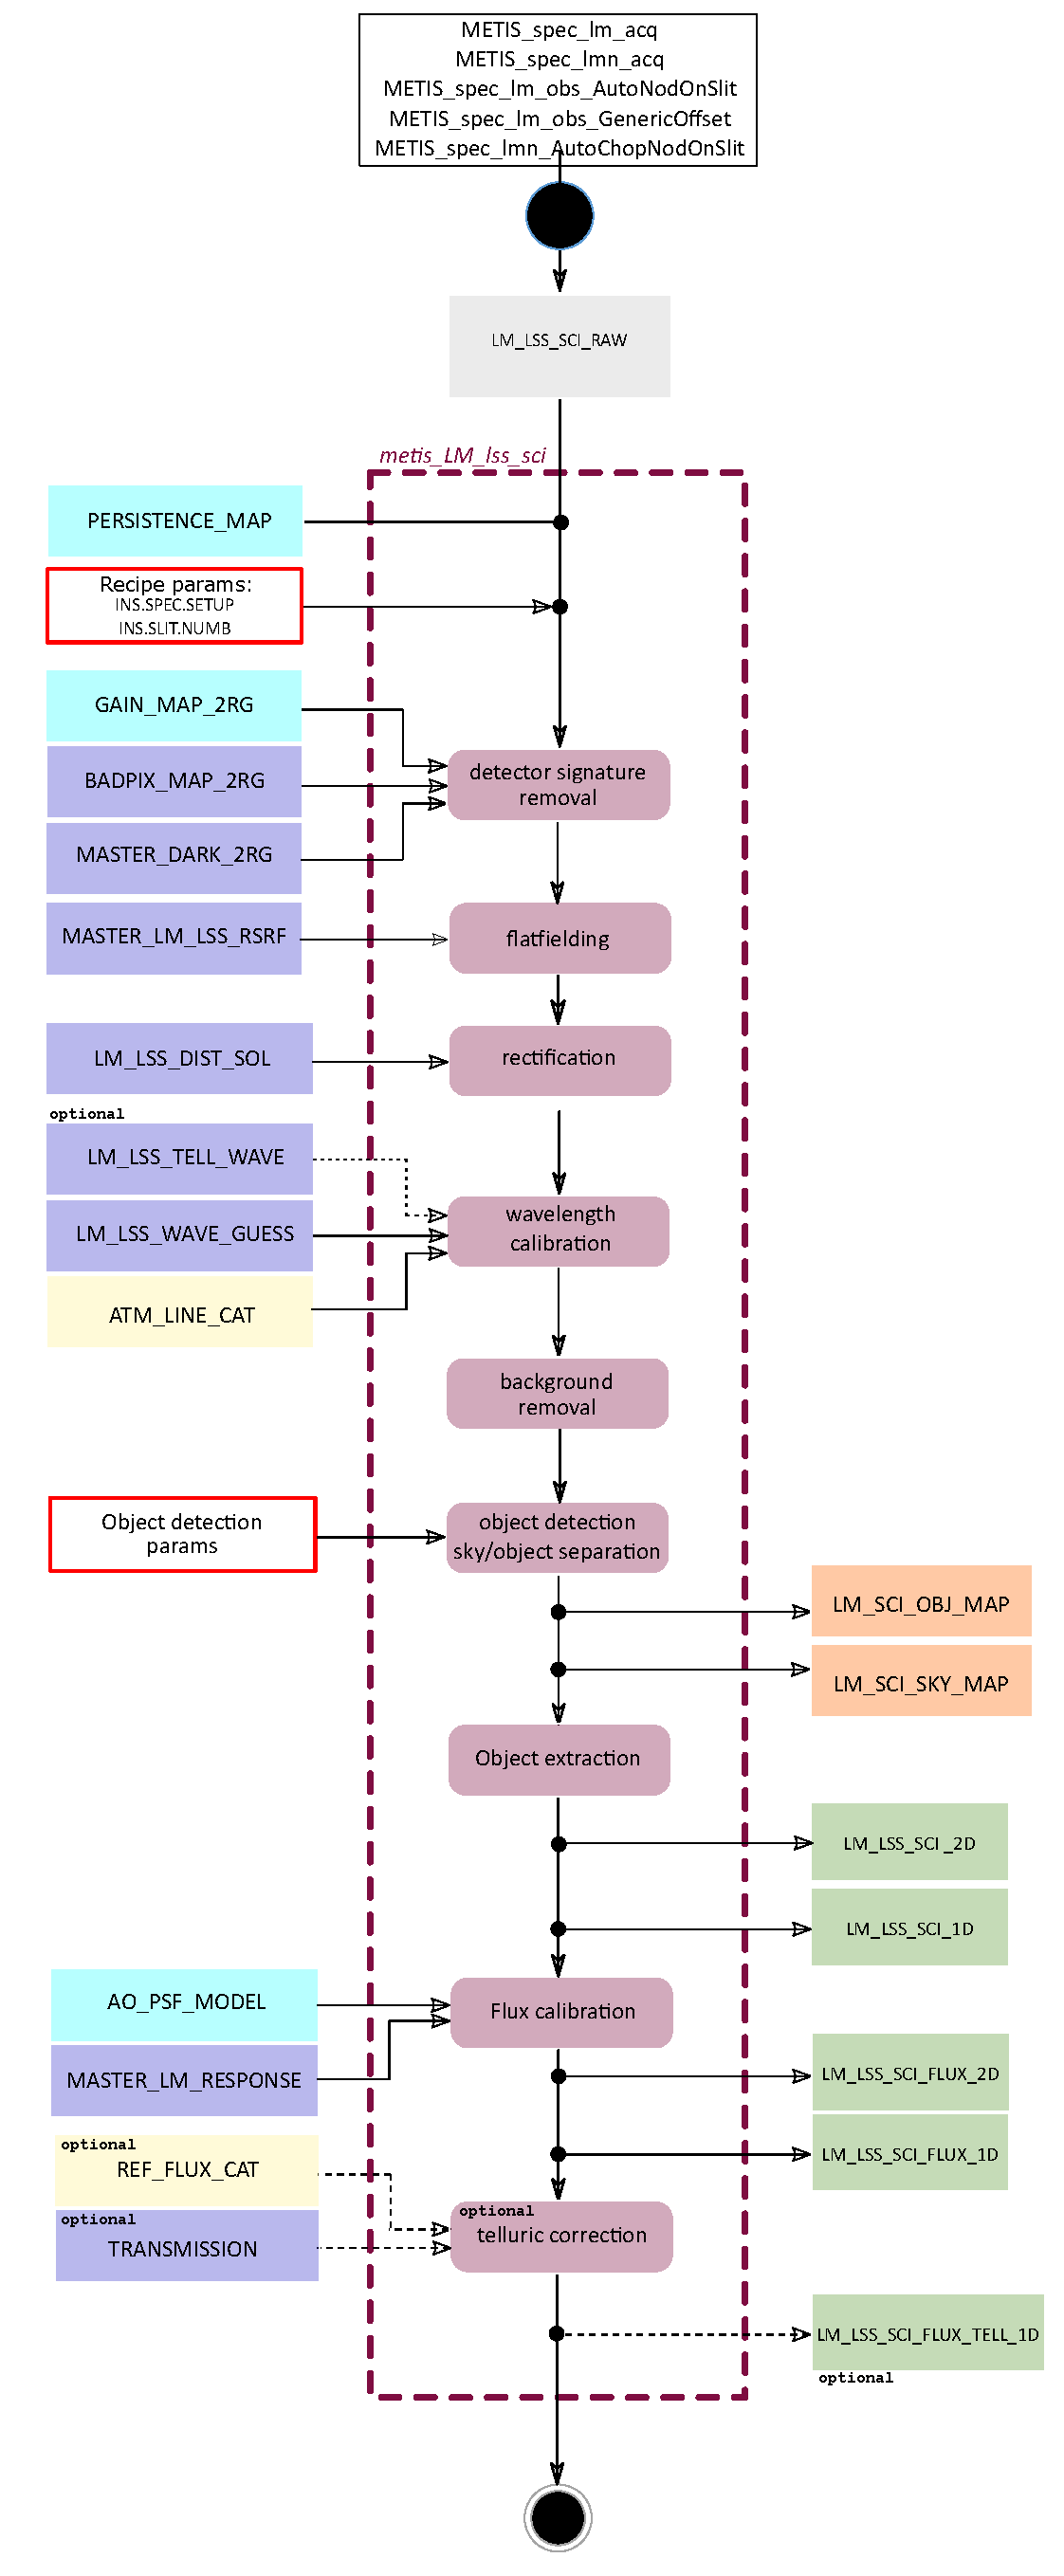
\includegraphics[width=0.37\textheight]{figures/metis_lm_lss_sci_v0.82.pdf}
  \caption[Recipe: \REC{metis_LM_lss_sci}]{\REC{metis_LM_lss_sci} --
    Science reduction recipe.}
  \label{Fig:rec_lm_lss_sci}
\end{figure}
\clearpage

\begin{recipedef}
Name:		& \hyperref[rec:metis_lm_lss_sci]{\REC{metis_LM_lss_sci}} \\
Purpose:    & Science data calibration\\
Type:		& Science reduction\\
Requirements: & METIS-6084 \\
Templates:           & \TPL{METIS_spec_lm_acq}, \\
                & \TPL{METIS_spec_lm_obs_AutoNodOnSlit}, \\
                & \TPL{METIS_spec_lm_obs_GenericOffset} \\
                & \TPL{METIS_spec_lm_cal_SlitAdc}\\
Input data: 	& \hyperref[dataitem:lm_lss_sci_raw]{\RAW{LM_LSS_SCI_RAW}}\\
                & \hyperref[dataitem:persistence_map]{\EXTCALIB{PERSISTENCE_MAP}}  \\
                & \hyperref[dataitem:gain_map_lm]{\STATCALIB{GAIN_MAP_LM}}  \\
                & \hyperref[dataitem:badpix_map_lm]{\PROD{BADPIX_MAP_LM}}  \\
                & \hyperref[dataitem:master_dark_lm]{\PROD{MASTER_DARK_LM}}  \\
                & \hyperref[dataitem:master_lm_lss_rsrf]{\PROD{MASTER_LM_LSS_RSRF}} \\
                & \hyperref[dataitem:lm_lss_dist_sol]{\PROD{LM_LSS_DIST_SOL}} \\
                & \hyperref[dataitem:lm_lss_wave_guess]{\PROD{LM_LSS_WAVE_GUESS}} \\
                & \hyperref[dataitem:atm_line_cat]{\EXTCALIB{ATM_LINE_CAT}} \\
                & \hyperref[dataitem:lm_adc_slitloss]{\STATCALIB{LM_ADC_SLITLOSS}}\\
            	& \hyperref[dataitem:std_transmission]{\PROD{STD_TRANSMISSION}} (optional)\\             
                %& \hyperref[dataitem:ao_psf_model]{\EXTCALIB{AO_PSF_MODEL}} \\
                %& \hyperref[dataitem:lsf_kernel]{\STATCALIB{LSF_KERNEL}}\\
                & \hyperref[dataitem:master_lm_response]{\PROD{MASTER_LM_RESPONSE}} \\
Parameters: 	& (TBD)\\
Algorithm:      & Application of the detector master calib files\\
                & wavelength calibration \\
                & Identifying/separatiing sky/object pixels\\
                & Removing sky lines: Creation and Subtraction of 2D sky\\
                & Coaddition of individual object spectra of one OB\\
                & Collapsing 2D to 1D spectrum, (see Fig.\,\ref{Fig:rec_lm_lss_sci})\\
                & Application of the response function (flux calibration) \\
Output data:	& \hyperref[dataitem:lm_lss_sci_obj_map]{\PROD{LM_LSS_SCI_OBJ_MAP}}: Pixel map of object pixels\\
            	& \hyperref[dataitem:lm_lss_sci_sky_map]{\PROD{LM_LSS_SCI_SKY_MAP}}: Pixel map of sky pixels\\
            	& \hyperref[dataitem:lm_lss_sci_2d]{\PROD{LM_LSS_SCI_2D}}: coadded, wavelength calibrated 2D spectrum\\
                & (\FITS{PRO_CATG}: \FITS{LM_LSS_2d_coadd_wavecal}) \\
                & \hyperref[dataitem:lm_lss_sci_1d]{\PROD{LM_LSS_SCI_1D}}: coadded, wavelength calibrated 1D spectrum\\
                & (\FITS{PRO_CATG}: \FITS{LM_LSS_1d_coadd_wavecal}) \\
                & \hyperref[dataitem:lm_lss_sci_flux_2d]{\PROD{LM_LSS_SCI_FLUX_2D}}: coadded, wavelength + flux calibrated 2D spectrum\\
                & (\FITS{PRO_CATG}: \FITS{LM_LSS_2d_coadd_wavecal}) \\
              	& \hyperref[dataitem:lm_lss_sci_flux_1d]{\PROD{LM_LSS_SCI_FLUX_1D}}: coadded, wavelength + flux 1D spectrum\\
                & (\FITS{PRO_CATG}: \FITS{LM_LSS_1d_coadd_wavecal}) \\
Expected accuracies: & (TBD)\\
QC1 parameters: & \hyperref[qc:lmlssscisnr]{\QC{QC LM LSS SCI SNR}}: Signal-to-noise ration of science spectrum\\
                & \hyperref[qc:lmlssscisnrnoise]{\QC{QC LM LSS SCI SNRNOISE}}: Noise level of science spectrum\\
                & \hyperref[qc:lmlssscifluxsnr]{\QC{QC LM LSS SCI FLUX SNR}}: Signal-to-noise ration of flux calibrated  science spectrum\\
                & \hyperref[qc:lmlssscifluxsnrnoise]{\QC{QC LM LSS SCI FLUX SNRNOISE}}: Noise level of flux calibrated science spectrum\\
                & \hyperref[qc:lmlsssciinterordrlevel]{\QC{QC LM LSS SCI INTORDR LEVEL}}: Flux level of the interorder background\\
                & \hyperref[qc:lmlsssciwavecaldevmean]{\QC{QC LM LSS SCI WAVECAL DEVMEAN}}: Mean deviation from the wavelength reference frame (TBDef)\\
                & \hyperref[qc:lmlsssciwavecalfwhm]{\QC{QC LM LSS SCI WAVECAL FWHM}}: Measured FWHM of lines\\
                & \hyperref[qc:lmlsssciwavecalnident]{\QC{QC LM LSS SCI WAVECAL NIDENT}}: Number of identified lines\\
                & \hyperref[qc:lmlsssciwavecalnmatch]{\QC{QC LM LSS SCI WAVECAL NMATCH}}: Number of lines matched between catalogue and spectrum\\
                & \hyperref[qc:lmlsssciwavecalpolydeg]{\QC{QC LM LSS SCI WAVECAL POLYDEG}}: Degree of the wavelength polynomial\\
                & \hyperref[qc:lmlsssciwavecalpolycoeffn]{\QC{QC LM LSS SCI WAVECAL POLYCOEFF\<n\>}}: $n$-th coefficient of the polynomial\\
                & more TBD\\
\end{recipedef}

\subsubsection{LM-LSS telluric correction recipe \REC{metis_LM_lss_mf_model}:}\label{rec:metis_lm_lss_mf_model}
The telluric correction will be done with the package \texttt{molecfit}\footnote{\url{https://www.eso.org/sci/software/pipelines/molecfit/molecfit-pipe-recipes.html}}. It is realised in three individual recipes, \hyperref[rec:metis_lm_lss_mf_model]{\REC{metis_LM_lss_mf_model}}, which calculates the best-fit model, \hyperref[rec:metis_lm_lss_mf_calctrans]{\REC{metis_LM_lss_mf_calctrans}}, which creates a synthetic transmission curve, and \hyperref[rec:metis_lm_lss_mf_correct]{\REC{metis_LM_lss_mf_correct}}, which performs the actual telluric correction by means of the synthetic transmission.

\begin{figure}[ht]
  \centering
  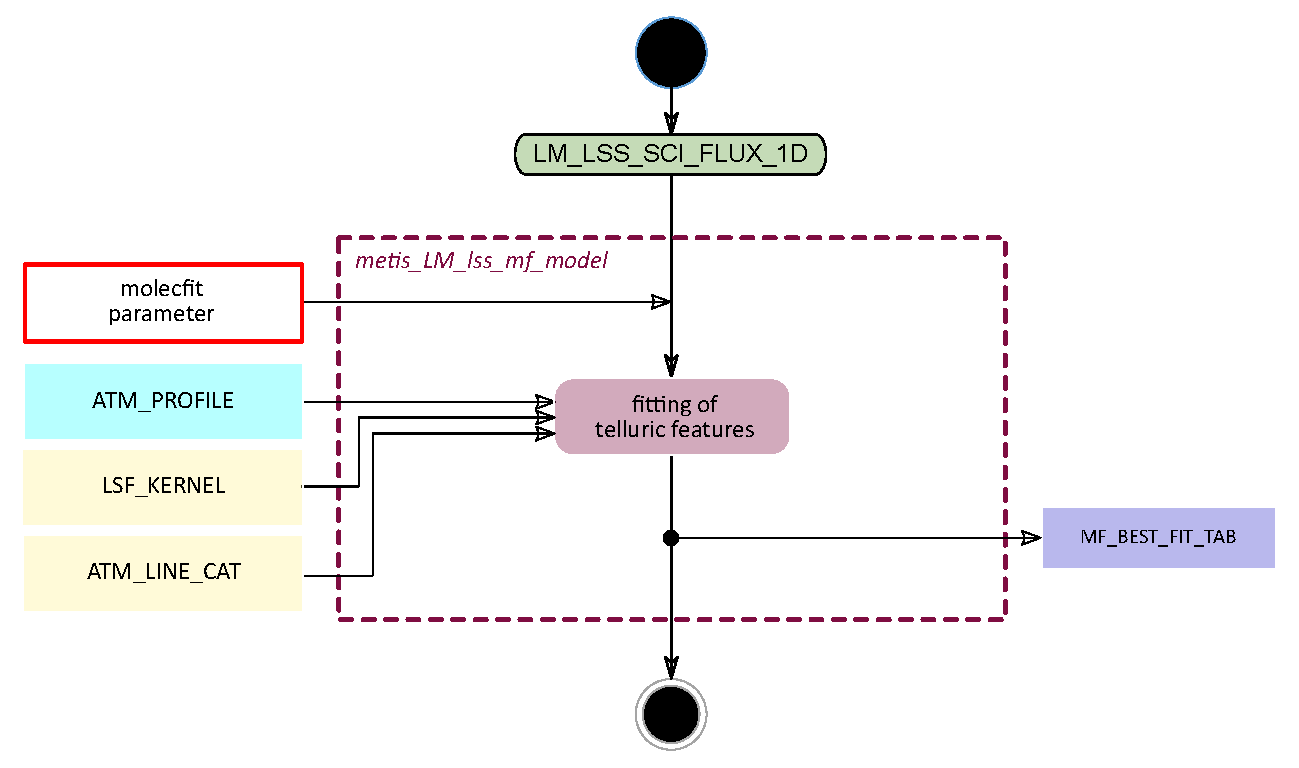
\includegraphics[width=0.5\textheight]{figures/metis_lm_lss_mf_model_v0.82.pdf}
  \caption[Recipe: \REC{metis_LM_lss_mf_model}]{\REC{metis_LM_lss_mf_model} --
    Recipe to achieve the best-fit for the calculation of the synthetic transmission curve for the telluric correction.}
  \label{Fig:rec_lm_lss_mf_model}
\end{figure}
\clearpage

\begin{recipedef}
Name:		& \hyperref[rec:metis_lm_lss_mf_model]{\REC{metis_LM_lss_mf_model}} \\
Purpose:	& Achieve the best fit for modelling the transmission curve to be applied as telluric correction \\
Type:		& Post-calibration\\
Requirements: & METIS-4051, METIS-6091 \\
Templates:           & None\\
Input data: 	& \hyperref[dataitem:lm_lss_sci_flux_1d]{\PROD{LM_LSS_SCI_FLUX_1D}}\\
                & \hyperref[dataitem:lsf_kernel]{\STATCALIB{LSF_KERNEL}} \\
                & \hyperref[dataitem:atm_profile]{\EXTCALIB{ATM_PROFILE}} \\
                & \hyperref[dataitem:atm_line_cat]{\EXTCALIB{ATM_LINE_CAT}} \\
Parameters: 	& \texttt{molecfit} parameters (c.f. \cite{molecfit})\\
Algorithm:      & Fit of telluric features visible in the science input spectrum\\
                & Determination of best-fit parameter set\\
Output data:	& \hyperref[dataitem:mf_best_fit_tab]{\PROD{MF_BEST_FIT_TAB}}: Table with best-fit parameters\\
Expected accuracies: & (TBD)\\
QC1 parameters: & cf. \cite{molecfit}\\
\end{recipedef}

\subsubsection{LM-LSS telluric correction recipe \REC{metis_LM_lss_mf_calctrans}:}\label{rec:metis_lm_lss_mf_calctrans}

\begin{figure}[ht]
  \centering
  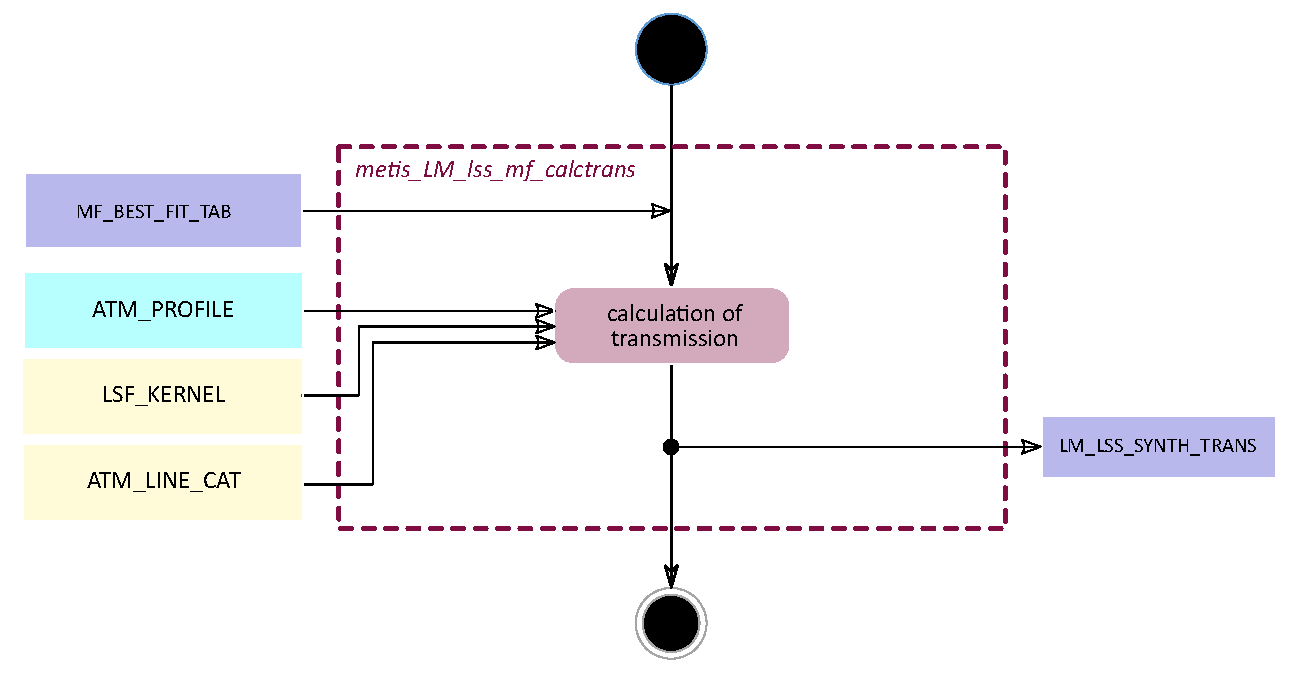
\includegraphics[width=0.5\textheight]{figures/metis_lm_lss_mf_calctrans_v0.82.pdf}
  \caption[Recipe: \REC{metis_LM_lss_mf_calctrans}]{\REC{metis_LM_lss_mf_calctrans} --
    Recipe to calculate the synthetic transmission to be applied as telluric correction.}
  \label{Fig:rec_lm_lss_mf_calctrans}
\end{figure}
\clearpage

\begin{recipedef}
Name:		& \hyperref[rec:metis_lm_lss_mf_calctrans]{\REC{metis_LM_lss_mf_calctrans}} \\
Purpose:	& Calculation of the synthetic transmission \\
Type:		& Post-calibration\\
Requirements: & METIS-4051, METIS-6091 \\
Templates:           & None\\
Input data: 	& \hyperref[dataitem:mf_best_fit_tab]{\PROD{MF_BEST_FIT_TAB}}: Table with best-fit parameters\\
                & \hyperref[dataitem:lsf_kernel]{\STATCALIB{LSF_KERNEL}} \\
                & \hyperref[dataitem:atm_profile]{\EXTCALIB{ATM_PROFILE}} \\
                & \hyperref[dataitem:atm_line_cat]{\EXTCALIB{ATM_LINE_CAT}} \\
Parameters: 	& \texttt{molecfit} parameters (c.f.  \cite{molecfit})\\
Algorithm:      & Calculate the entire transmission curve by means of the best-fit parameters\\
Output data:	& \hyperref[dataitem:lm_lss_synth_trans]{\PROD{LM_LSS_SYNTH_TRANS}}: synth. transmission\\
Expected accuracies: & (TBD)\\
QC1 parameters: & cf. \cite{molecfit}\\
\end{recipedef}

\subsubsection{LM-LSS telluric correction recipe \REC{metis_LM_lss_mf_correct}:}\label{rec:metis_lm_lss_mf_correct}

\begin{figure}[ht]
  \centering
  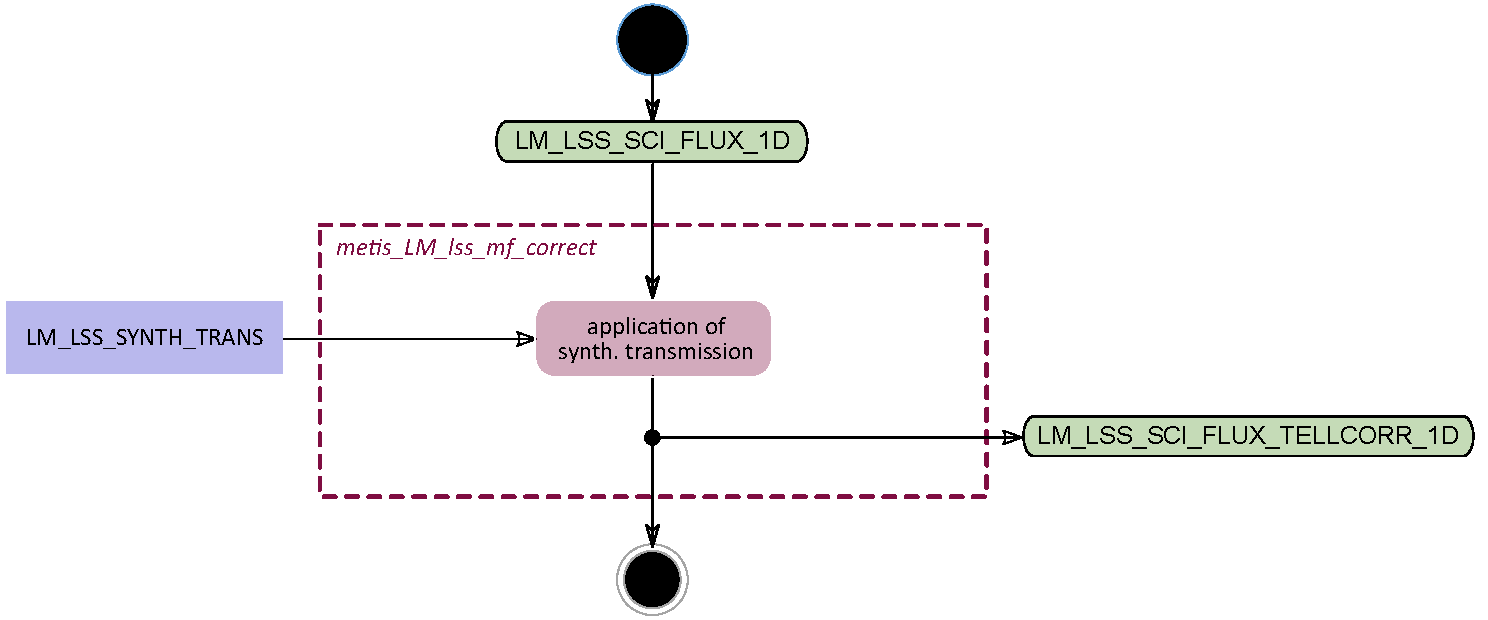
\includegraphics[width=0.5\textheight]{figures/metis_lm_lss_mf_correct_v0.82.pdf}
  \caption[Recipe: \REC{metis_LM_lss_mf_correct}]{\REC{metis_LM_lss_mf_correct} --
    Recipe to apply the telluric correction.}
  \label{Fig:rec_lm_lss_mf_correct}
\end{figure}
\clearpage

\begin{recipedef}
Name:		& \hyperref[rec:metis_lm_lss_mf_correct]{\REC{metis_LM_lss_mf_correct}} \\
Purpose:	& Apply the synthetic transmission to the science spectra \\
Type:		& Post-calibration\\
Requirements: & METIS-4051, METIS-6091 \\
Templates:           & None\\
Input data: 	& \hyperref[dataitem:lm_lss_sci_flux_1d]{\PROD{LM_LSS_SCI_FLUX_1D}}\\
                & \hyperref[dataitem:lm_lss_synth_trans]{\PROD{LM_LSS_SYNTH_TRANS}}\\
Parameters: 	& None\\
Algorithm:      & Apply telluric correction, i.e. divide the input science spectrum\\
                & by the synthetic transmission\\
Output data:	& \hyperref[dataitem:lm_lss_sci_flux_tellcorr_1d]{\PROD{LM_LSS_SCI_FLUX_TELLCORR_1D}}\\
Expected accuracies: & (TBD)\\
QC1 parameters: & cf. \cite{molecfit}\\
\end{recipedef}




\clearpage
\subsection{N-band long-slit spectroscopy recipes}
\label{ssec:recipes_lss_n}
A draft of the reduction cascade is shown in Figs.~\ref{Fig:NLssAssomap1} and \ref{Fig:NLssAssomap2}.% together with the data processing table (Tables~\ref{Tab:NLssDatProc1} and ~\ref{Tab:NLssDatProc2}). 
The first part aims to update the static calibration database, in particular the creation of the gain map (\REC{metis_det_lingain}) and the determination of the \ac{ADC} slitlosses (\REC{metis_n_adc_slitloss}). Both are executed only when an update is required, e.g. after a major instrument interention or on yearly basis. The second part comprises the basic calibrations, e.g. the dark correction and the spectroscopic flatfielding via \ac{RSRF}, followed by the third part, the main calibration steps, incorporating the wavelength calibration (by means of atmospheric lines visible in the respective spectra and the first guess wavelength solution created during \ac{AIT}) and the determination of the response curve for the flux calibration. Therefore the main step of the wavelength calibration is carried out in the recipes \REC{metis_N_lss_std} and \REC{metis_LM_lss_sci}. Finally, the telluric absorption correction is applied using the modelling approach with \texttt{molecfit}.
%------------------------------------------------------------------------------------------------------------------
%\subsubsection{Recipes \REC*{metis_det_lingain} and \REC*{metis_det_dark}}
These recipes aim for detector-specific calibrations and are therefore the same as in the imaging pipeline. Common detector calibrations are described in Section~\ref{Sec:detector_calibration}.\\
Note that the list of \ac{QC} parameters in the recipe descriptions will be extended whenever necessary.\\
%------------------------------------------------------------------------------------------------------------------
\subsubsection{\REC*{metis_det_lingain} and \REC*{metis_det_dark}: Linearity/Gain}
These recipes aim for detector-specific calibrations and are therefore the same as in the imaging pipeline. Common detector calibrations are described in Section~\ref{Sec:detector_calibration}.

%------------------------------------------------------------------------------------------------------------------
\subsubsection{\REC*{metis_N_adc_slitloss}: Slit loss determination}
The recipe \REC{metis_n_adc_slitloss} aims to determine the slit losses induced by atmospheric refraction. The recipe aims to create a table with slitlosses (\STATCALIB{N_ADC_SLITLOSS}), which is added to the static database and used in the recipes \REC{metis_N_lss_std}. This recipe is to be carried out only when an update of the database is needed. The algorithm and the workflow of the recipe to determine the slitlosses is given in Section~\ref{sssec:adc_slitlosses}, more information can be found in Section "Calibration of slit losses" in the Calibration Plan~\cite{METIS-calibration_plan}. 

%------------------------------------------------------------------------------------------------------------------
\subsubsection{\REC*{metis_N_lss_rsrf}:  Flatfielding}\label{rec:metis_n_lss_rsrf}
The recipe \REC{metis_N_lss_rsrf} aims to create a spectroscopic master flatfield for determining the pixel-to-pixel sensitivity and to enable the order location algorithm (\REC{metis_N_lss_trace}).
\begin{figure}[ht]
  \centering
  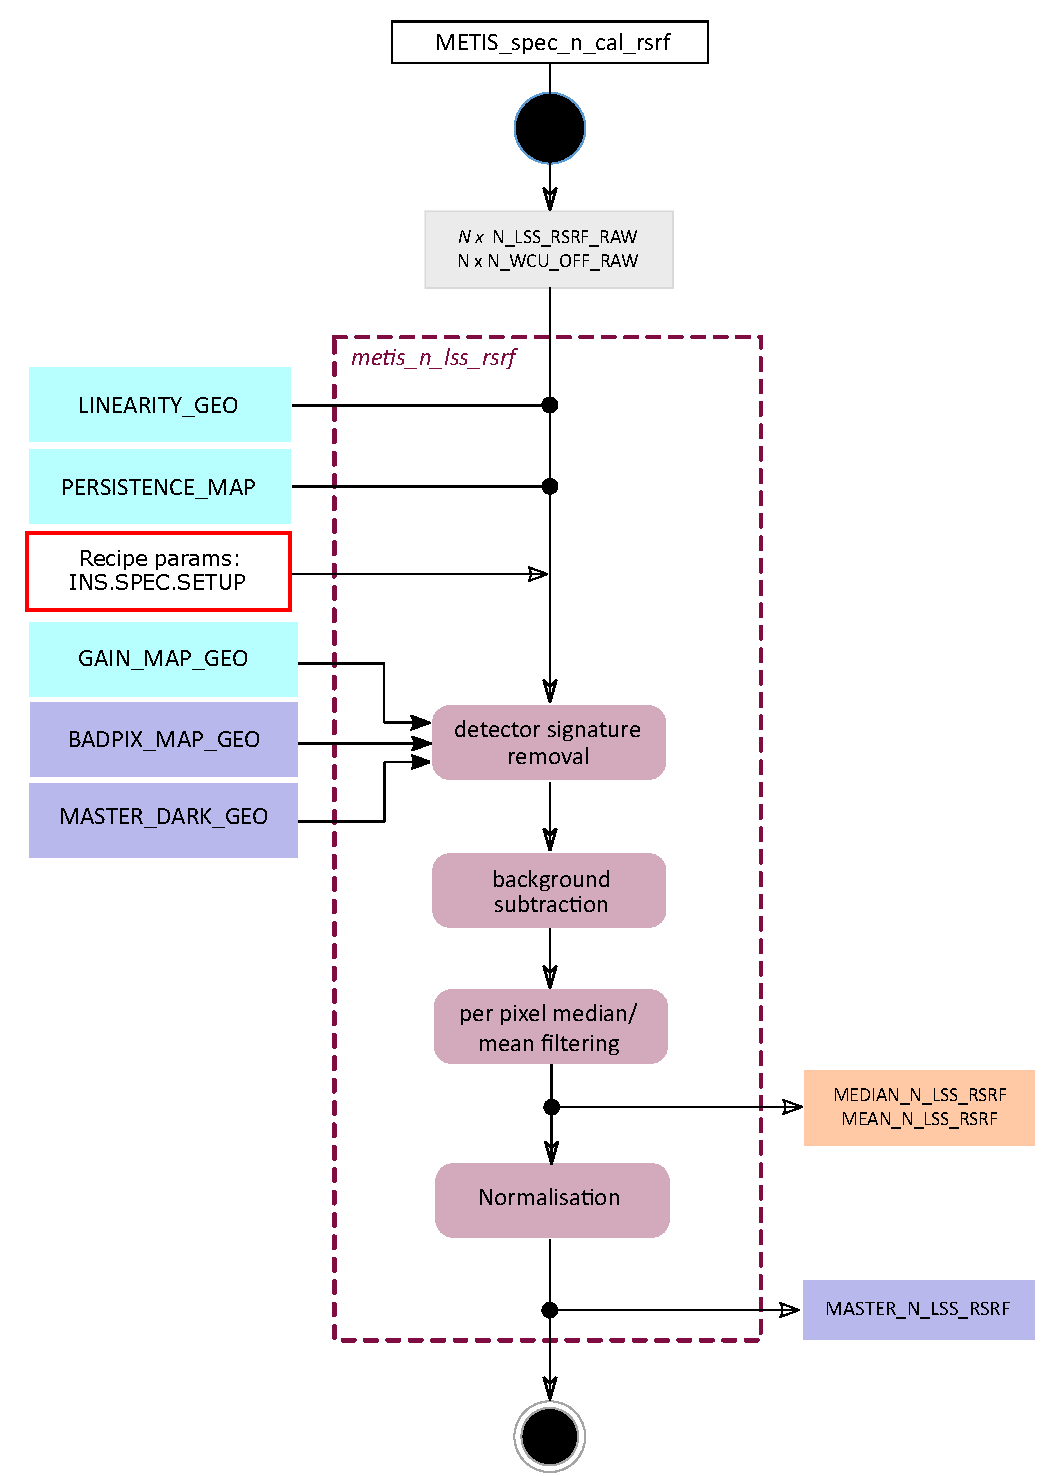
\includegraphics[width=0.5\textheight]{figures/metis_n_lss_rsrf_v0.84.pdf}
  \caption[Recipe: \REC*{metis_N_lss_rsrf}]{\REC*{metis_N_lss_rsrf} --
    Spectroscopic faltfielding with \ac{RSRF}.}
  \label{Fig:rec_n_lss_rsrf}
\end{figure}

\begin{recipedef}
Name:		& \REC{metis_N_lss_rsrf} \\
Purpose:	& Spectroscopic flatfielding with \ac{RSRF} \\
Type:		& Calibration\\
Requirements: & METIS-6084, METIS-3291, METIS-9099 \\
Templates:           & \TPL{METIS_spec_n_cal_rsrf} \\
Input data:     & $N\times$ \RAW{N_LSS_RSRF_RAW} \\
                & $N\times$ \RAW{N_WCU_OFF_RAW} \\
                & \EXTCALIB{PERSISTENCE_MAP}  \\
                & \STATCALIB{LINEARITY_GEO}  \\
                & \STATCALIB{GAIN_MAP_GEO}  \\
                & \EXTCALIB{BADPIX_MAP_GEO}   \\
                & \PROD{MASTER_DARK_GEO}  \\
Matched Keywords & \FITS{DET.DIT} \\
                 & \FITS{DET.NDIT}\\
                 & \FITS{DRS.SLIT}\\
Parameters: 	& exposure time\\
Algorithm:      & subtract master \ac{WCU} "OFF" frame from illumination frame (done on individual images)\\
                & median/mean filtering of subtracted images\\
                & division by blackbody spectrum\\
                & normalisation to achieve \ac{RSRF}\\
Output data:	&  \PROD{MASTER_N_LSS_RSRF} (\FITS{PRO.CATG}=\CODE{MASTER_N_LSS_TRSRF}): master flatfield/\ac{RSRF} \\
                & \PROD{MEDIAN_N_LSS_RSRF_IMG}: median map (\ac{QC})\\
                & \PROD{MEAN_N_LSS_RSRF_IMG}: mean map (\ac{QC})\\

Expected accuracies: & 3\% (cf.~\cite{METIS-calibration_plan} and~\cite{METIS_calerrbudget})\\
QC1 parameters: & \QC{QC N LSS RSRF MEAN LEVEL}: Mean level of the \ac{RSRF}\\
                & \QC{QC N LSS RSRF MEDIAN LEVEL}: Median level of the \ac{RSRF}\\
                & \QC{QC N LSS RSRF INTORDR LEVEL}: Flux level of the interorder background\\
                & \QC{QC N LSS RSRF NORM STDEV}: Standard deviation of the normalised \ac{RSRF}\\
                & \QC{QC N LSS RSRF NORM SNR}: \ac{SNR} of the normalised \ac{RSRF}\\
%                & more TBD\\
\end{recipedef}
%------------------------------------------------------------------------------------------------------------------
\clearpage
\subsubsection{\REC*{metis_N_lss_trace}:  Order detection}\label{rec:metis_n_lss_trace}
The recipe \REC{metis_N_lss_trace} aims at detecting the order and a polynomial fitting of the order location (see~\cite{pis02} and~\cite{pis21} for details on the algorithms). The detection and polynomial fitting is based on flatfield frames taken through a pinhole mask, which leads to individual pinhole traces along the entire dispersion direction.

\begin{figure}[ht]
  \centering
  \includegraphics[width=0.5\textheight]{figures/metis_N_lss_trace_v0.84.pdf}
  \caption[Recipe: \REC*{metis_N_lss_trace}]{\REC*{metis_N_lss_trace} --
    Detection and polynomial fitting of the order location.}
  \label{Fig:rec_N_lss_wave}
\end{figure}

\begin{recipedef}
Name:		& \REC{metis_N_lss_trace} \\
Purpose:	& Detection of order location \\
Type:		& Calibration\\
Requirements: & None \\
Templates:           & \TPL{METIS_spec_n_cal_rsrfpinh} \\
Input data:     & $N\times$ \RAW{N_LSS_RSRF_PINH_RAW} \\
                $N\times$ \RAW{N_WCU_OFF_RAW} \\
                & \EXTCALIB{PERSISTENCE_MAP}  \\
                & \STATCALIB{LINEARITY_GEO}  \\
                & \STATCALIB{GAIN_MAP_GEO}  \\
                & \EXTCALIB{BADPIX_MAP_GEO}   \\
                & \PROD{MASTER_DARK_GEO}  \\
                &  \PROD{MASTER_N_LSS_RSRF} \\
Matched Keywords & \FITS{DET.DIT} \\
                 & \FITS{DET.NDIT}\\
                 & \FITS{DRS.SLIT}\\
Parameters: 	& exposure time\\
Algorithm:      & Detection of the order edges\\
                & Polynomial fitting\\
Output data:	& \PROD{N_LSS_TRACE} (\FITS{PRO.CATG}=\CODE{N_LSS_TRACE}): Polynomial coefficients\\
Expected accuracies: & 1/10th of a pixel after post-processing\\
               & (cf.~\cite{METIS-calibration_plan}, R-MET-106, METIS-167, METIS-1371)\\
QC1 parameters: & \QC{QC N LSS TRACE LPOLYDEG}: Degree of the polynomial fit of the left order edge\\
                & \QC{QC N LSS TRACE LCOEFF<i>}: $i$-th coefficient of the polynomial of the left order edge\\
                & \QC{QC N LSS TRACE RPOLYDEG}: Degree of the polynomial fit of the right order edge\\
                & \QC{QC N LSS TRACE RCOEFF<i>}: $i$-th coefficient of the polynomial of the right order edge\\
                & \QC{QC N LSS TRACE INTORDR LEVEL}: Flux level of the interorder background\\
%                & \QC{TBD}: TBD\\
\end{recipedef}

\clearpage

%------------------------------------------------------------------------------------------------------------------
\subsubsection{\REC*{metis_N_lss_std}:  Standard star processing}\label{rec:metis_n_lss_std}
This recipe aims at processing standard stars used for the absolute flux calibration and (optionally) for the telluric feature removal: As first step the detector master calibration files derived previously are applied followed by the background subtraction, if needed the distortion correction (\PROD{N_LSS_DIST_SOL}), and
the wavelength calibration by means of the first guess solution (\PROD{N_LSS_WAVE_GUESS}) and the telluric sky lines (c.f. Sect.\,8.5 in~\cite{DRLS}). Then the recipe removes sky background, extracts the standard star spectrum object and collapses the 2D to 1D spectra. In case the \ac{STD} is used only for the flux calibration, a telluric correction is required to better compare the corresponding model spectrum. This is done by means of the standard star observations itself or (optionally) with a synthetic transmission curve (either a standard curve derived by the ESO Skycalc Tool\footnote{\url{https://www.eso.org/observing/etc/bin/gen/form?INS.MODE=swspectr+INS.NAME=SKYCALC}}, a standard curve (\STATCALIB{N_SYNTH_TRANS}) or \texttt{molecfit}. It is on the user's decision whether the standard star is used for the absolute flux calibration only, or also used for the telluric correction of the science target. The response function is then calculated as ratio of the measured 1d-\ac{STD} spectrum and a detailed model containing absolute flux information.

Please note that the procedure of the \ac{STD} handling changes when the classical method for the telluric correction is chosen. The reason is that in the response function, also the telluric features of the \ac{STD} star have to be present to be able to apply a combination of the telluric absorption removal and the conversion towards physical flux units (cf. Section~\ref{ssec:tellcorr}). In the case of using \texttt{molecfit}, a telluric correction is applied to the \ac{STD} spectrum to better determine the response function and only the response is delivered to the science recipes. In case of the classical approach with a \ac{STD}, the response function will also contain the telluric features of the \ac{STD}, and therefore a telluric correction beforehand is counterproductive.\\

\begin{figure}[ht]
  \centering
  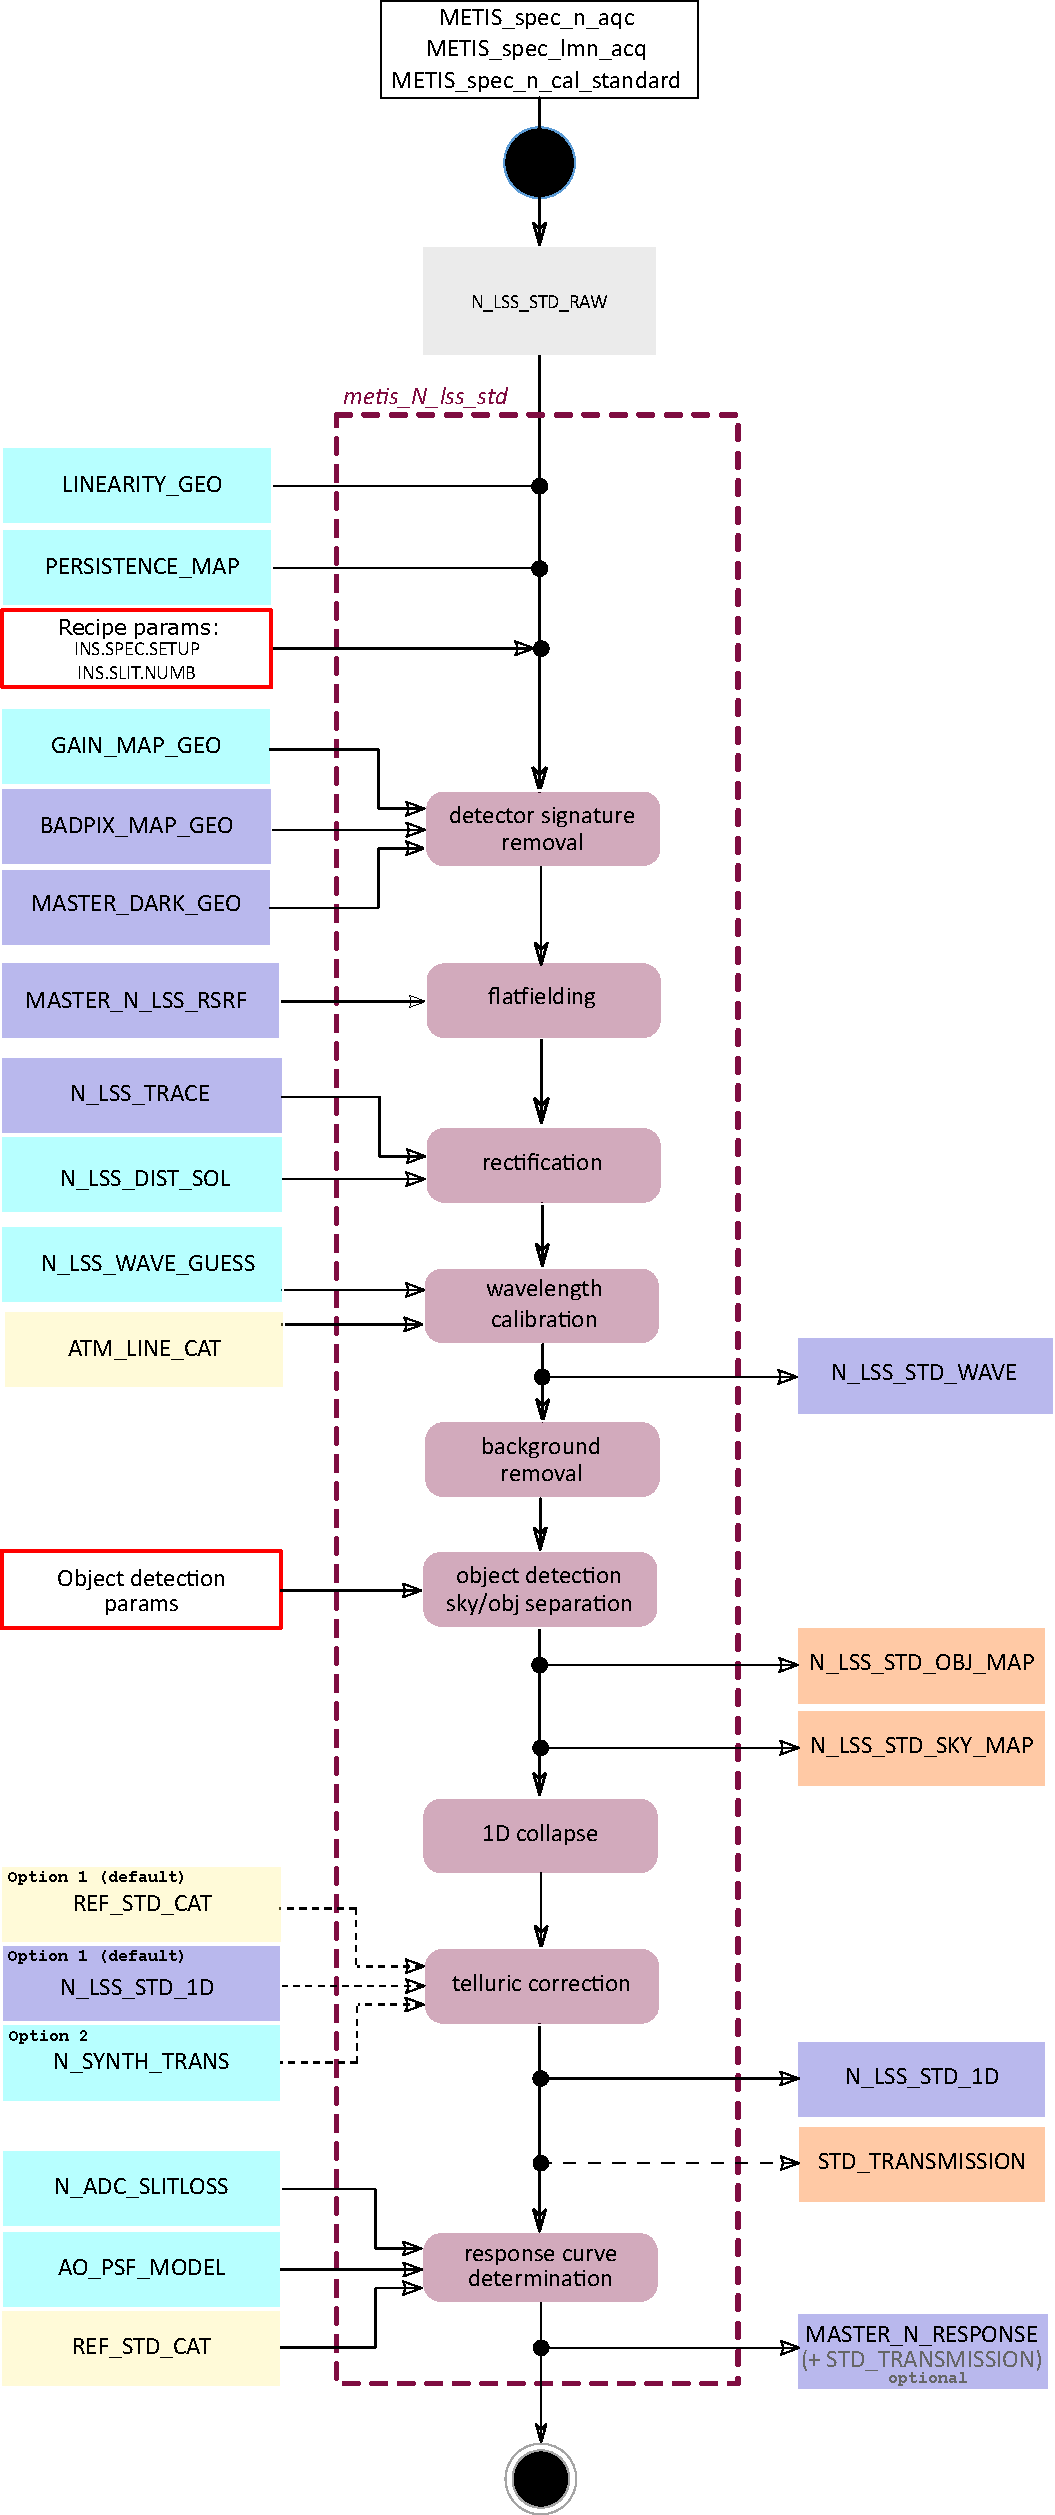
\includegraphics[width=0.4\textheight]{figures/metis_n_lss_std_v0.83.pdf}
  \caption[Recipe: \REC*{metis_N_lss_std}]{\REC*{metis_N_lss_std} --
    Standard star calibration recipe.}
  \label{Fig:rec_N_lss_flux}
\end{figure}
\clearpage
\begin{recipedef}
Name:		& \REC{metis_N_lss_std} \\
Purpose:	& Flux calibration \\
Type:		& Calibration\\
Requirements: & METIS-6084, METIS-6074, METIS-2757 \\
Templates:      & \TPL{METIS_spec_n_acq}, \\
                & \TPL{METIS_spec_lmn_acq}, \\
                & \TPL{METIS_spec_N_cal_standard}\\
                & \TPL{METIS_spec_lmn_obs_AutoChopNodOnSlit}\\
Input data: 	& \RAW{N_LSS_STD_RAW}\\
                & \EXTCALIB{PERSISTENCE_MAP}  \\
                & \STATCALIB{LINEARITY_GEO}  \\
                & \STATCALIB{GAIN_MAP_GEO}  \\
                & \EXTCALIB{BADPIX_MAP_GEO}   \\
                & \PROD{MASTER_DARK_GEO}  \\
                & \PROD{MASTER_N_LSS_RSRF} \\
                & \PROD{N_LSS_TRACE}\\
                & \STATCALIB{N_LSS_DIST_SOL} \\
                & \STATCALIB{N_LSS_WAVE_GUESS} \\
                & \STATCALIB{N_SYNTH_TRANS}\\
                & \EXTCALIB{AO_PSF_MODEL} \\
                & \EXTCALIB{ATM_LINE_CAT} \\
                & \STATCALIB{N_ADC_SLITLOSS}\\
                & \STATCALIB{REF_STD_CAT} \\                
Matched Keywords & \FITS{DET.DIT} \\
                 & \FITS{DET.NDIT}\\
                 & \FITS{DRS.SLIT}\\
Parameters: 	& exposure time, target information, nodding(/chopping parameters\\
Algorithm:      & Application of master calibration files\\
                & Determination and application of the wavelength solution\\
                & Background removal\\
                & Determination and application of the distortion correction\\
                & Identifying/separatiing sky/object pixels\\
                & Removing telluric lines\\
                & Collapsing 2D to 1D spectrum, (see Fig.\,\ref{Fig:rec_N_lss_sci})\\
                & Determination and application of response curve\\
Output data:	& \PROD{N_LSS_STD_OBJ_MAP}: Pixel map of object pixels (\ac{QC})\\
            	& \PROD{N_LSS_STD_SKY_MAP}: Pixel map of sky pixels (\ac{QC})\\
              	& \PROD{N_LSS_STD_1D}  : coadded, wavelength calibrated, collapsed 1D spectrum\\
                & \PROD{STD_TRANSMISSION}: Transmission curve derived by menas of the \ac{STD} star (\ac{QC})\\
                & \PROD{MASTER_N_RESPONSE}: response function (optionally including the transmission)\\
Expected accuracies: & for wavelength: 1/10th of a pixel after post-processing\\
            & (cf.~\cite{METIS-calibration_plan}, R-MET-106, METIS-167, METIS-1371)\\
            & for flux: 10\% over an atmospheric band \\
            & $<30$\% absolute line flux accuracy\\
            & $<5$\% absolute flux calibration \\
            & (cf.~\cite{METIS-calibration_plan}, R-MET-107, R-MET-82)\\
QC1 parameters: & \QC{QC N LSS STD BACKGD MEAN}: Mean value of background\\
                & \QC{QC N LSS STD BACKGD MEDIAN}: Median value of background\\
                & \QC{QC N LSS STD BACKGD STDEV}: Standard deviation value of background\\
                & \QC{QC N LSS STD SNR}: Signal-to-noise ration of flux standard star spectrum\\
                & \QC{QC N LSS STD NOISELEV}: Noise level of flux standard star spectrum\\
                & \QC{QC N LSS STD FWHM}: FWHM of flux standard spectrum\\
                & \QC{QC N LSS STD INTORDR LEVEL}: Flux level of the interorder background\\
                & \QC{QC N LSS STD AVGLEVEL}: Average level of the standard star flux \\
                & \QC{QC N LSS STD WAVECAL DEVMEAN}: Mean deviation from the
                  wavelength reference frame\\
                & \QC{QC N LSS STD WAVECAL FWHM}: Measured FWHM of lines\\
                & \QC{QC N LSS STD WAVECAL NIDENT}: Number of identified lines\\
                & \QC{QC N LSS STD WAVECAL NMATCH}: Number of lines matched between
                    catalogue and spectrum\\
                & \QC{QC N LSS STD WAVECAL POLYDEG}: Degree of the polynomial\\
                & \QC{QC N LSS STD WAVECAL POLYCOEFF<n>}: $n$-th coefficient of the polynomial\\
                & \QC{QC N LSS STD SNR}: Signal-to-noise ration of flux standard star spectrum\\
                & \QC{QC N LSS STD NOISELEV}: Noise level of flux standard star spectrum\\
                & \QC{QC N LSS STD FWHM}: FWHM of flux standard spectrum\\
%                & \QC{QC N LSS STD PSFLOSS}: Fraction of AO induced slit losses (TBdef)\\
%                & more TBD\\
\end{recipedef}

%------------------------------------------------------------------------------------------------------------------
\clearpage
\subsubsection{\REC*{metis_N_lss_sci}:  Science reduction}\label{rec:metis_n_lss_sci}
The science calibration recipe comprises the extraction of the object (i.e. separation of object/sky pixels), removing the sky lines, the application of the response curve previously defined. In case of a point/compact source, the 2D to 1D collapse is also done, otherwise 2D products are delivered. Finally, the spectra are coadded. The recipe also applies an absolute flux calibration (optionally with the telluric correction in one step, cf. Section~\ref{ssec:tellcorr}).
\begin{figure}[ht]
  \centering
  \includegraphics[width=0.35\textheight]{figures/metis_N_lss_sci_v0.83.pdf}
  \caption[Recipe: \REC*{metis_N_lss_sci}]{\REC*{metis_N_lss_sci} --
    Science reduction recipe.}
  \label{Fig:rec_N_lss_sci}
\end{figure}
\clearpage

\begin{recipedef}
Name:		& \REC{metis_N_lss_sci} \\
Purpose:  & Science data calibration\\
Type:		& Science reduction\\
Requirements: & METIS-6084 \\
Templates:      & \TPL{METIS_spec_n_acq}, \\
                & \TPL{METIS_spec_lmn_acq}, \\
                & \TPL{METIS_spec_n_obs_AutoChopNodOnSlit}, \\
                & \TPL{METIS_spec_lmn_obs_AutoChopNodOnSlit}\\
% HB 20230627 Template METIS_spec_N_obs_GenericOffset does not exist
%                 & \TPL{METIS_spec_N_obs_GenericOffset} \\
%                & \TPL{METIS_spec_n_cal_slit}\\
Input data: 	& \RAW{N_LSS_SCI_RAW}\\
                & \EXTCALIB{PERSISTENCE_MAP}  \\
                & \STATCALIB{LINEARITY_GEO}  \\
                & \STATCALIB{GAIN_MAP_GEO}  \\
                & \EXTCALIB{BADPIX_MAP_GEO}   \\
                & \PROD{MASTER_DARK_GEO}  \\
                & \PROD{MASTER_N_LSS_RSRF} \\
                & \PROD{N_LSS_TRACE}\\
                & \STATCALIB{N_LSS_DIST_SOL}\\
                & \STATCALIB{N_LSS_WAVE_GUESS}\\
                & \EXTCALIB{ATM_LINE_CAT} \\
                %& \EXTCALIB{AO_PSF_MODEL} \\
                & \STATCALIB{N_ADC_SLITLOSS}\\
                & \PROD{MASTER_N_RESPONSE} \\
Matched Keywords & \FITS{DET.DIT} \\
                 & \FITS{DET.NDIT}\\
                 & \FITS{DRS.SLIT}\\
Parameters: 	& exposure time, target information, nodding(/chopping parameters\\
Algorithm:      & Application of the detector master calib files\\
                & wavelength calibration \\
                & Identifying/separatiing sky/object pixels\\
                & Removing sky lines: Creation and Subtraction of 2D sky\\
                & Coaddition of individual object spectra of one OB\\
                & Collapsing 2D to 1D spectrum, (see Fig.\,\ref{Fig:rec_N_lss_sci})\\
                & Application of the response function (flux calibration) \\
Output data:	& \PROD{N_LSS_SCI_OBJ_MAP}: Pixel map of object pixels (\ac{QC})\\
            	& \PROD{N_LSS_SCI_SKY_MAP}: Pixel map of sky pixels (\ac{QC})\\
            	& \PROD{N_LSS_SCI_2D}: coadded, wavelength calibrated 2D spectrum\\
                & (\FITS{PRO.CATG}: \CODE{N_LSS_2d_coadd_wavecal}) \\
                & \PROD{N_LSS_SCI_1D}: coadded, wavelength calibrated 1D spectrum\\
                & (\FITS{PRO.CATG}: \CODE{N_LSS_1d_coadd_wavecal}) \\
                & \PROD{N_LSS_SCI_FLUX_2D}: coadded, wavelength calibrated 2D spectrum\\
                & (\FITS{PRO.CATG}: \CODE{N_LSS_2d_coadd_wavecal}) \\
              	& \PROD{N_LSS_SCI_FLUX_1D}: coadded, wavelength 1D spectrum\\
                & (\FITS{PRO.CATG}: \CODE{N_LSS_1d_coadd_wavecal}) \\
Expected accuracies: & for wavelength: 1/10th of a pixel after post-processing\\
            & (cf.~\cite{METIS-calibration_plan}, R-MET-106, METIS-167, METIS-1371)\\
            & for flux: 10\% over an atmospheric band \\
            & $<30$\% absolute line flux accuracy\\
            & $<5$\% absolute flux calibration \\
            & (cf.~\cite{METIS-calibration_plan}, R-MET-107, R-MET-82)\\
            & for optional telluric correction: 10\% within an atmospheric band); desired: 2\% 
            (\cite{METIS-calibration_plan})\\
QC1 parameters: & \QC{QC N LSS SCI SNR}: Signal-to-noise ration of science spectrum\\
                & \QC{QC N LSS SCI NOISELEV}: Noise level of science spectrum\\
                & \QC{QC N LSS SCI FLUX SNR}: Signal-to-noise ration of flux calibrated  science spectrum\\
                & \QC{QC N LSS SCI FLUX NOISELEV}: Noise level of flux calibrated science spectrum\\
                & \QC{QC N LSS SCI INTORDR LEVEL}: Flux level of the interorder background\\
                & \QC{QC N LSS SCI WAVECAL DEVMEAN}: Mean deviation from the wavelength reference frame\\
                & \QC{QC N LSS SCI WAVECAL FWHM}: Measured FWHM of lines\\
                & \QC{QC N LSS SCI WAVECAL NIDENT}: Number of identified lines\\
                & \QC{QC N LSS SCI WAVECAL NMATCH}: Number of lines matched between catalogue and spectrum\\
                & \QC{QC N LSS SCI WAVECAL POLYDEG}: Degree of the wavelength polynomial\\
                & \QC{QC N LSS SCI WAVECAL POLYCOEFF<n>}: $n$-th coefficient of the polynomial\\
%                & more TBD\\
\end{recipedef}

%------------------------------------------------------------------------------------------------------------------
\clearpage
\subsubsection{\REC*{metis_N_lss_mf_model}:  Telluric correction}\label{rec:metis_n_lss_mf_model}
The telluric correction will be done with the package \texttt{molecfit}\footnote{\url{https://www.eso.org/sci/software/pipelines/molecfit/molecfit-pipe-recipes.html}}. It is realised in three individual recipes, \REC{metis_N_lss_mf_model}, which calculates the best-fit model, \REC{metis_N_lss_mf_calctrans}, which creates a synthetic transmission curve, and \REC{metis_N_lss_mf_correct}, which performs the actual telluric correction by means of the synthetic transmission.

\begin{figure}[ht]
  \centering
  \includegraphics[width=0.5\textheight]{figures/metis_N_lss_mf_model_v0.83.pdf}
  \caption[Recipe: \REC*{metis_N_lss_mf_model}]{\REC*{metis_N_lss_mf_model} --
    Recipe to achieve the best-fit for the calculation of the synthetic transmission curve for the telluric correction.}
  \label{Fig:rec_N_lss_mf_model}
\end{figure}
\clearpage

\begin{recipedef}
Name:		& \REC{metis_N_lss_mf_model}\\
Purpose:	& Achieve the best fit for modelling the transmission curve to be applied as telluric correction \\
Type:		& Post-calibration\\
Requirements: & METIS-4051, METIS-6091 \\
Templates:           & None\\
Input data: 	& \PROD{N_LSS_SCI_FLUX_1D}\\
                & \STATCALIB{LSF_KERNEL} \\
                & \EXTCALIB{ATM_PROFILE} \\
                & \EXTCALIB{ATM_LINE_CAT} \\
Matched Keywords & \FITS{DRS.SLIT}\\
Parameters: 	& \texttt{molecfit} parameters (c.f. \cite{molecfit})\\
Algorithm:      & Fit of telluric features visible in the science input spectrum\\
                & Determination of best-fit parameter set\\
Output data:	& \PROD{MF_BEST_FIT_TAB}\\
Expected accuracies: & n/a\\
QC1 parameters: & cf.~\cite{molecfit}\\
\end{recipedef}

%------------------------------------------------------------------------------------------------------------------
\clearpage
\subsubsection{\REC*{metis_N_lss_mf_calctrans}:  Telluric correction}\label{rec:metis_n_lss_mf_calctrans}
\begin{figure}[ht]
  \centering
  \includegraphics[width=0.5\textheight]{figures/metis_N_lss_mf_calctrans_v0.83.pdf}
  \caption[Recipe: \REC*{metis_N_lss_mf_calctrans}]{\REC*{metis_N_lss_mf_calctrans} --
    Recipe to calculate the synthetic transmission to be applied as telluric correction.}
  \label{Fig:rec_N_lss_mf_calctrans}
\end{figure}
\clearpage

\begin{recipedef}
Name:		& \REC{metis_N_lss_mf_calctrans}\\
Purpose:	& Calculation of the synthetic transmission \\
Type:		& Post-calibration\\
Requirements: & METIS-4051, METIS-6091 \\
Templates:           & None\\
Input data: 	& \PROD{MF_BEST_FIT_TAB}\\
                & \STATCALIB{LSF_KERNEL} \\
                & \EXTCALIB{ATM_PROFILE} \\
                & \EXTCALIB{ATM_LINE_CAT} \\
Matched Keywords & \FITS{DRS.SLIT}\\
Parameters: 	& \texttt{molecfit} parameters (c.f.  \cite{molecfit})\\
Algorithm:      & Calculate the entire transmission curve by means of the best-fit parameters\\
Output data:	& \PROD{N_LSS_SYNTH_TRANS}\\
\\
Expected accuracies: & n/a\\
QC1 parameters: & cf.~\cite{molecfit}\\
\end{recipedef}

%------------------------------------------------------------------------------------------------------------------
\clearpage
\subsubsection{\REC*{metis_N_lss_mf_correct}:  Telluric correction}\label{rec:metis_n_lss_mf_correct}
\begin{figure}[ht]
  \centering
  \includegraphics[width=0.5\textheight]{figures/metis_N_lss_mf_correct_v0.83.pdf}
  \caption[Recipe: \REC*{metis_N_lss_mf_correct}]{\REC*{metis_N_lss_mf_correct} --
    Recipe to apply the telluric correction.}
  \label{Fig:rec_N_lss_mf_correct}
\end{figure}
\clearpage

\begin{recipedef}
Name:		& \REC{metis_N_lss_mf_correct}\\
Purpose:	& Apply the synthetic transmission to the science spectra \\
Type:		& Post-calibration\\
Requirements: & METIS-4051, METIS-6091 \\
Templates:           & None\\
Input data: 	& \PROD{N_LSS_SCI_FLUX_1D}\\
                & \PROD{N_LSS_SYNTH_TRANS}\\
Matched Keywords & \FITS{DRS.SLIT}\\
Parameters: 	& None\\
Algorithm:      & Apply telluric correction, i.e. divide the input science spectrum\\
                & by the synthetic transmission\\
Output data:	& \PROD{N_LSS_SCI_FLUX_TELLCORR_1D}\\
Expected accuracies: & Telluric removal must be good enough to reach the required spectro-photometric accuracy (10\% within an atmospheric band). Desired: 2\% (\cite{METIS-calibration_plan})\\
QC1 parameters: & cf.~\cite{molecfit}\\
\end{recipedef}








%% 06_5-Recipes_IFU.tex
%% Created:     Fri Aug 25 13:14:02 2017 by Koehler@I-Mac
%%
%% subsection for IFU recipes
%%
%%%%%%%%%%%%%%%%%%%%%%%%%%%%%%%%%%%%%%%%%%%%%%%%%%%%%%%%%%%%%%%%%%%%%%%%%%%%%%%

\clearpage
\subsection{LM integral-field spectroscopy (IFU)}
\label{ssec:IFU_recipes}

\TODO{This section is identical to the PDR document \cite{DRLS}. We
will consider rearranging the recipes to be in line with the imaging
pipelines. This would entail handling basic reduction and background
subtraction for both science and standard exposures in common
recipes (\CODE{metis_ifu_basic}, \CODE{metis_ifu_background}), then
having a recipe to analyse the standard observations
(\CODE{metis_ifu_photstd}). The science exposures are then fully
calibrated (\REC{metis_ifu_calibrate}). A full set of exposures would
then be assembled and restored with a fully sampled PSF in a
post-processing recipe (\CODE{metis_ifu_combine}).}

\subsubsection{IFU wavelength calibration}
\label{sssec:ifu_wavecal}
\label{rec:metis_ifu_wavecal}

This recipe processes daytime wavelength calibration images to derive
the pixel-to-wavelength relation for the LM integral-field
spectrograph. The calibration template will use the \ac{QCL} in the warm calibration unit to finely sample the desired
wavelength range. The image will consist of lines for each wavelength
and slice. The solution will have to provide for each detector pixel
$(x,y)$ the slice number $i$, the spatial position $\xi$ along the
slice and the wavelength in the dispersion correction. As the slices
and wavelength lines may be tilted with respect to the detector
columns and rows, a combined solution is required
\begin{eqnarray}
  \label{eq:wavelength_solution}
  \xi &= f_{i}(x, y) \\
  \lambda &= g_{i}(x, y)
\end{eqnarray}
The boundaries of the slice image on the detector are obtained by
measuring the left and right edges of the wavelength lines and
interpolating. The slice number is then obtained by counting the
slices according to the optical design of the spectrograph. The
wavelength of each line is known from the settings of the \ac{QCL}, the $x$
coordinate is obtained by linear interpolation along the line (or
perhaps using the distortion table from \hyperref[rec:metis_ifu_distortion]{\REC{metis_ifu_distortion}} if
necessary). The functions $f_{i}$ and $g_{i}$ are expected to be
sufficiently accurately described by low-order polynomials.

The recipe produces a multi-extension FITS file with an image
extension mapping wavelength across each detector in the array. A
table extension holds the polynomial coefficients.

 This is in compliance with \REQ{METIS-6074}.

\begin{recipedef}
  Name:                & \hyperref[rec:metis_ifu_wavecal]{\REC{metis_ifu_wavecal}}              \\
  Purpose:             & Determine pixel-to-wavelength transformation.                          \\
  Requirements:        & \REQ{METIS-6074}                                                       \\
  Type:                & Calibration                                                            \\
  Templates:           & \TPL{METIS_ifu_cal_InternalWave}                                       \\
  Input data:          & Images taken with WCU \ac{QCL} source                                  \\
                       & \hyperref[dataitem:master_dark_ifu]{\PROD{MASTER_DARK_IFU}}            \\
                       & Bad-pixel map                                                          \\
                       & Distortion table (TBD)                                                 \\
  Parameters:          & TBD                                                                    \\
  Algorithm:           & Measure line locations (left and right edges, centroid by Gaussian fit)\\
                       & Compute wavelength solution $\xi(x, y, i)$, $\lambda(x, y, i)$         \\
  Output data:         & \hyperref[dataitem:ifu_wavecal]{\PROD{IFU_WAVECAL}}                    \\
  Expected accuracies: & TBD                                                                    \\
  QC1 parameters:      & \QC{QC IFU WAVECAL RMS}                                                \\
                       & \QC{QC IFU WAVECAL NLINES}                                             \\
                       & \QC{QC IFU WAVECAL PEAK CNTS}                                          \\
                       & \QC{QC IFU WAVECAL LINE WIDTH}                                         \\
  \end{recipedef}

\begin{figure}[hb]
  \centering
  \includegraphics[width=0.7\textwidth]{metis_ifu_wavecal}
  \caption[Recipe: \REC{metis_ifu_wavecal}]{\REC{metis_ifu_wavecal} --
    daytime wavelength calibration for the IFU.}
  \label{fig:metis_ifu_wavecal}
\end{figure}


\clearpage
\subsubsection{IFU relative spectral response function}
\label{sssec:ifu_rsrf}
\label{rec:metis_ifu_rsrf}

This recipe creates a spectroscopic master flat and determines the
relative spectral response function (RSRF) for the four HAWAII2RG
detectors of the LM spectrograph. The input data are obtained by
illuminating the field of view with the black-body calibration lamp at
two different temperatures. The RSRF is then determined by dividing
the image by the known lamp continuum shape for the respective
temperature. We refer to the two-dimensional image obtained by this
division as \hyperref[dataitem:master_flat_ifu]{\PROD{MASTER_FLAT_IFU}} and the one-dimensional reponse
function obtained by averaging at constant wavelength as
\PROD{RSRF}. The bad pixel mask can be updated by identifying pixels
that deviate strongly from their neighbours.

\begin{recipedef}
Name:                & \hyperref[rec:metis_ifu_rsrf]{\REC{metis_ifu_rsrf}}                                                     \\
Purpose:             & Create relative spectral response function for the IFU detector.         \\
Requirements:        & \REQ{METIS-6131}, \REQ{METIS-6698}                                       \\
Type:                & Calibration                                                              \\
Templates:           & \TPL{METIS_ifu_cal_rsrf}                                                 \\
Input data:          & Raw flats taken with black-body calibration lamp.                        \\
                     & \hyperref[dataitem:master_dark_ifu]{\PROD{MASTER_DARK_IFU}}              \\
                     & \hyperref[dataitem:badpix_map_ifu]{\PROD{BADPIX_MAP_IFU}}                                                    \\
                     & \hyperref[dataitem:ifu_wavecal]{\PROD{IFU_WAVECAL}}: image with wavelength at each pixel.                 \\
Parameters:          & TBD                                                                      \\
Algorithm:           & Create continuum image by mapping Planck spectrum at $T_{\mathrm{lamp}}$ to
                       wavelength image.                                                        \\
                     & Divide exposures by continuum image.                                     \\
                     & Average exposures to yield master flat (2D RSRF).                        \\
                     & Average in spatial direction to obtain relative response function        \\
Output data:         & \hyperref[dataitem:master_flat_ifu]{\PROD{MASTER_FLAT_IFU}}                                                   \\
                     & \hyperref[dataitem:rsrf_ifu]{\PROD{RSRF_IFU}}                                                          \\
                     & \hyperref[dataitem:badpix_map_ifu]{\PROD{BADPIX_MAP_IFU}}                                                    \\
Expected accuracies: & TBD                                                                      \\
QC1 parameters:      & \QC{QC IFU RSRF NBADPIX}                                                    \\
                     & (more TBD)                                                               \\
\end{recipedef}

\begin{figure}[hb]
  \centering
  \includegraphics[width=0.6\textwidth]{metis_ifu_rsrf}
  \caption[Recipe: \REC{metis_ifu_rsrf}]{\REC{metis_ifu_rsrf} --
    creation of IFU relative spectral response function.}
  \label{fig:metis_ifu_rsrf}
\end{figure}


\clearpage
\subsubsection{IFU flux standard reduction}
\label{sssec:ifu_std_process}
\label{rec:metis_ifu_std_process}

This recipe reduces and analyses a series of IFU observations of a
spectroscopic flux standard star. The comparison of the measured
detector counts (ADU) with the tabulated spectrum of the star gives
the wavelength-dependent conversion from ADU to physical units
(photons per second per per centimetre square per wavelength bin per
spatial bin).

The level of stray light is estimated in the dark areas between the
spectra and subtracted from the entire frame. The distribution of
stray light across the field can only be characterised once the
instrument is built. It is to be hoped that subtraction of a constant
or a low-level 2D polynomial fit will be sufficient.

The sky and thermal background is estimated from blank sky
observations (if obtained during the observing sequence) or by
combining the (dithered) science frames.

The wavelength calibration is taken from the daylight calibration. It
may be refined by measuring telluric emission and/or absorption lines
(by fitting with \lstinline{molecfit}).

\begin{recipedef}
  Name:                & \hyperref[rec:metis_ifu_std_process]{\REC{metis_ifu_std_process}}                                            \\
  Purpose:             & Determine conversion between detector counts and physical source flux. \\
  Requirements:        & \REQ{METIS-6131}                                                       \\
  Type:                & Calibration                                                            \\
  Templates:           & \TPL{METIS_ifu_cal_standard}                                           \\
  Input data:          & Raw spectra of flux standard star                                      \\
                       & \hyperref[dataitem:master_dark_ifu]{\PROD{MASTER_DARK_IFU}}            \\
                       & Master flat (2D relative spectral response function)                   \\
                       & Bad pixel mask                                                         \\
                       & Wavelength calibration image                                           \\
                       & Distortion table                                                       \\
  Parameters:          & TBD                                                                    \\
  Algorithm:           & Subtract dark, divide by master flat                                   \\
                       & Estimate stray light and subtract                                      \\
                       & Estimate background and subtract                                       \\
                       & Rectify spectra and assemble cube                                      \\
                       & Extract 1D spectrum of star                                            \\
                       & Compute and apply telluric correction                                  \\
                       & Compute conversion to physical units as function of wavelength.        \\
  Output data:         & \hyperref[dataitem:ifu_std_reduced_cube]{\PROD{IFU_STD_REDUCED_CUBE}}  \\
                       & \hyperref[dataitem:ifu_std_background_cube]{\PROD{IFU_STD_BACKGROUND_CUBE}}                                         \\
                       & \hyperref[dataitem:ifu_std_reduced_1d]{\PROD{IFU_STD_REDUCED_1D}}                                              \\
                       & \hyperref[dataitem:ifu_std_telluric_1d]{\PROD{IFU_STD_TELLURIC_1D}}                                             \\
                       & \hyperref[dataitem:fluxcal_tab]{\PROD{FLUXCAL_TAB}}                                                     \\
  Expected accuracies: & TBD                                                                    \\
  QC1 parameters:      & \QC{QC IFU STD STRAYLIGHT MEAN}                                        \\
\end{recipedef}

\begin{figure}[hb]
  \centering
  \includegraphics[width=0.7\textwidth]{metis_ifu_std_process}
  \caption[Recipe: \REC{metis_ifu_std_process}]{%
    \hyperref[rec:metis_ifu_std_process]{\REC{metis_ifu_std_process}} -- reduction of IFU flux standard
    frames and flux calibration (not all data products are shown).}
  \label{fig:metis_ifu_std_process}
\end{figure}

\clearpage
\subsubsection{IFU science reduction}
\label{sssec:ifu_sci_process}
\label{rec:metis_ifu_sci_process}

This recipe performs basic reduction of raw science exposures applying
dark and RSRF correction and flux calibration (i.e.~conversion of
pixel values to physical units) on each exposure individually. The
recipe shall be able to process data from either the nominal or the
extended wavelength mode. For the nominal mode, all slices belong to
the same echelle order. For the extended mode, slices belonging to the
same echelle order are grouped and processing is iterated over the
echelle orders.

The level of stray light is estimated in the dark areas between the
spectra and subtracted from the entire frame. The distribution of
stray light across the field can only be characterised once the
instrument is built. It is to be hoped that subtraction of a constant
or a low-level 2D polynomial fit will be sufficient.

The sky and thermal background, as well as residual straylight, is
estimated from blank sky observations if these are available in the
sequence of input frames or by combining (dithered) science
frames. The initial wavelength solution is taken from the daylight
calibration. It may be checked and corrected by measuring atmospheric
lines if a sufficient number is available in the limited wavelength
range.

A telluric correction is determined by this recipe by automatically
extracting a 1D spectrum from ``object'' pixels identified by a
thresholding algorithm. \lstinline{molecfit} is applied to this
spectrum and the correction is mapped back to the reduced 2D images or
3D cubes using the wavelength images. In an interactive environment
(Reflex workflow) the telluric correction may be improved by asking
the user to define an extraction aperture adapted to the target
structure.

Various levels of output data can be envisaged:
\begin{itemize}
\item Reduced 2D detector images. These are accompanied by additional
  information describing the geometry of the slice layout, target
  position and wavelength calibration to the extent that the exposure can be
  combined with other exposures into a single rectified spectral cube.
  This information can be stored in the FITS header or a table
  extension.
\item A rectified spectral cube for each exposure with a linear
  wavelength grid, constructed by resampling each spectral slice onto
  a spatial-wavelength grid common to all slices. The spatial pixels
  are rectangular with along-slit pixel scale given by the detector
  pixel scale and the across-slit pixel scale given by the slice
  width.
\item A spectral cube obtained by combining all exposures taken within
  a template. This step involves the image reconstruction discussed in
  Sect.~8.9 of \cite{DRLS}. Whether this step is included
  in the present recipe \hyperref[rec:metis_ifu_sci_process]{\REC{metis_ifu_sci_process}} or is postponed to
  the more general recipe \hyperref[rec:metis_ifu_sci_postprocess]{\REC{metis_ifu_sci_postprocess}} is TBD. It
  may be formally required to do the image reconstruction here if
  templates are set up to obtain a fixed set of spatially dithered and
  rotated exposures aimed at reconstructing a fully sampled PSF in
  both spatial dimensions.
\end{itemize}

For the nominal mode, each output is a single-extension FITS file
corresponding to one echelle order. For the extended mode, each of the
echelle orders results in an extension in a multi-extension FITS
file.

The recipe as descibed here is run in the science pipelines. For the
observatory pipeline, a variant of the recipe may be implemented with
reduced functionality and output. The observatory recipe may also have
to include features to determine QC parameters for the LM-band images
that are taken in parallel with the IFU exposures, similar to
\REC{metis_lm_img_sci_process} (Sect.~\ref{ssec:recipes_img_lm}).

\begin{recipedef}
Name:                & \hyperref[rec:metis_ifu_sci_process]{\REC{metis_ifu_sci_process}}                                                              \\
Purpose:             & Reduction of individual science exposures.                                               \\
Requirements:        & \REQ{METIS-6131}                                                                         \\
Type:                & Science                                                                                  \\
Templates:           & \TPL{METIS_ifu_obs_FixedSkyOffset}                                                       \\
                     & \TPL{METIS_ifu_obs_GenericOffset}                                                        \\
                     & \TPL{METIS_ifu_ext_obs_FixedSkyOffset}                                                   \\
                     & \TPL{METIS_ifu_ext_obs_GenericOffset}                                                    \\
% TODO: Decide what to do about app
%                     & \TPL{METIS_ifu_app_obs_GenericOffset}                                                    \\
                     & \TPL{METIS_ifu_vc_obs_FixedSkyOffset}                                                    \\
%                     & \TPL{METIS_ifu_ext_app_obs_GenericOffset}                                                \\
                     & \TPL{METIS_ifu_ext_vc_obs_FixedSkyOffset}                                                \\
                     & \TPL{METIS_ifu_cal_psf}                                                                  \\
Input data:          & Dithered science exposures.                                                              \\
                     & Blank sky images (if available)                                                          \\
                     & \hyperref[dataitem:master_dark_ifu]{\PROD{MASTER_DARK_IFU}}                              \\
                     & Master flat (2D relative spectral response function)                                     \\
                     & Bad pixel mask                                                                           \\
                     & Wavelength calibration image                                                             \\
                     & Flux calibration table                                                                   \\
                     & Distortion table                                                                         \\
                     & Line spread kernel to be used with \CODE{molecfit}                                       \\
Parameters:          & telluric correction (yes/no)                                                             \\
                     & more TBD                                                                                 \\
Algorithm:           & Subtract dark, divide by master flat                                                     \\
                     & Estimate stray light and subtract                                                        \\
                     & Estimate background from dithered science exposures or blank-sky exposures and subtract. \\
                     & Apply flux calibration.                                                                  \\
                     & Rectify spectra and assemble cube                                                        \\
                     & Extract 1D object spectrum                                                               \\
                     & Compute telluric correction and apply to reduced images and cube                         \\
Output data:         & \hyperref[dataitem:ifu_sci_reduced]{\PROD{IFU_SCI_REDUCED}} (2D, per exposure)           \\
                     & \hyperref[dataitem:ifu_sci_reduced_tac]{\PROD{IFU_SCI_REDUCED_TAC}} (2D, per exposure)   \\
                     & \hyperref[dataitem:ifu_sci_background]{\PROD{IFU_SCI_BACKGROUND}} (2D, per exposure)     \\
                     & \hyperref[dataitem:ifu_sci_reduced_cube]{\PROD{IFU_SCI_REDUCED_CUBE}} (3D, per exposure) \\
                     & \hyperref[dataitem:ifu_sci_reduced_cube_tac]{\PROD{IFU_SCI_REDUCED_CUBE_TAC}} (3D, per exposure) \\
                     & \hyperref[dataitem:ifu_sci_combined]{\PROD{IFU_SCI_COMBINED}} (3D)                       \\
                     & \hyperref[dataitem:ifu_sci_combined_tac]{\PROD{IFU_SCI_COMBINED_TAC}} (3D)               \\
                     & \hyperref[dataitem:ifu_sci_object_1d]{\PROD{IFU_SCI_OBJECT_1D}}  (1D)                    \\
                     & \hyperref[dataitem:ifu_sci_telluric_1d]{\PROD{IFU_SCI_TELLURIC_1D}}                      \\
Expected accuracies: & TBD                                                                                      \\
QC1 parameters:      & TBD                                                                                      \\
\end{recipedef}

\begin{figure}[hb]
  \centering
  \includegraphics[width=0.7\textwidth]{metis_ifu_sci_process}
  \caption[Recipe: \REC{metis_ifu_sci_process}]{%
    \hyperref[rec:metis_ifu_sci_process]{\REC{metis_ifu_sci_process}} -- reduction of IFU science frames.}
  \label{fig:metis_ifu_sci_process}
\end{figure}



\clearpage
\subsubsection{IFU telluric absorption correction}
\label{sssec:ifu_tellcorr}
\label{rec:metis_ifu_tellcorr}

This recipe corrects for telluric absorption in a reduced IFU data
cube. The correction is done via a model atmospheric spectrum derived
with \CODE{molecfit}.

An automatic telluric correction can be performed as part of
\REC{metis_ifu_sci_process}. In an interactive environment it may be
better to do the telluric correction as a separate post-processing
step with a user-defined aperture for the extraction of a 1D object
spectrum. The spectrum is extracted from a combined cube
(\PROD{IFU_SCI_COMBINED}) but may be applied to other products of
\REC{metis_ifu_sci_process} specified in the input set of frames.

\begin{recipedef}
  Name:                & \hyperref[rec:metis_ifu_tellcorr]{\REC{metis_ifu_tellcorr}}                                                        \\
  Purpose:             & Remove telluric absorption features                                             \\
  Requirements:        & \REQ{METIS-6091}                                                                \\
  Type:                & Calibration / post processing                                                   \\
  Templates:           & ---                                                                             \\
  Input data:          & \hyperref[dataitem:ifu_sci_combined]{\PROD{IFU_SCI_COMBINED}} -- reduced combined IFU cube                            \\
                       & \hyperref[dataitem:lsf_kernel]{\STATCALIB{LSF_KERNEL}} -- Line spread kernel to be used with \CODE{molecfit}         \\
                       & \hyperref[dataitem:atm_profile]{\EXTCALIB{ATM_PROFILE}} -- Atmospheric input profile to be used with \CODE{molecfit} \\
  Parameters:          & extraction aperture parameters                                                  \\
                       & \CODE{molecfit} parameters                                                      \\
                       & atmospheric profile incl.\ radiometer data                                      \\
                       & line spread kernel                                                              \\
  Algorithm:           & extract 1D spectrum                                                             \\
                       & Application of molecfit                                                         \\
  Output data:         & \hyperref[dataitem:ifu_sci_reduced_tac]{\PROD{IFU_SCI_REDUCED_TAC}}                                                      \\
  Expected accuracies: & TBD                                                                             \\
  QC1 parameters:      & TBD                                                                             \\
\end{recipedef}

\begin{figure}[hb]
  \centering
  \includegraphics[width=0.7\textwidth]{metis_ifu_tellcorr}
  \caption[Recipe: \REC{metis_ifu_tellcorr}]{\REC{metis_ifu_tellcorr}
    -- telluric correction of reduced IFU science cubes.}
  \label{fig:metis_ifu_tellcorr}
\end{figure}


\clearpage
\subsubsection{IFU science postprocessing}
\label{sssec:ifu_sci_postprocess}
\label{rec:metis_ifu_sci_postprocess}

This recipe combines a number of reduced IFU exposures covering a
different spatial and wavelength ranges into a single data cube. The
positions and orientations of the exposures may differ as follows: \TODO{Reference to operational concept}
\begin{description}
\item[Spatial dithering:] The target is placed at different positions
  along and across the slice. Along-slice dithering aids in background
  subtraction, across-slice dithering is necessary image
  reconstruction given that the slice width undersamples the PSF.
\item[Field rotation:] The field is rotated by 90 degrees between
  exposures. The cube of a single exposure has different pixel scales
  along and across the slice. The goal of combining exposures at
  different rotation angles is to reconstruct images on a square grid
  with pixel scale given by the detector scale (8.2\,mas). The exact
  procedure remains to be investigated; one of the major challenges is
  to find the exact centre of rotation
  (Sect.~8.9 of \cite{DRLS}).
\item[Spectral dithering:] Sequences of exposures are taken at various
  echelle angles in order to cover an increased contiguous wavelength
  range. In the extended mode, such a sequence may cover the
  wavelength gaps between echelle order coverage.
\end{description}

In order to allow co-addition of data from separate OBs, possibly taken
months apart, the wavelengths will be corrected to the heliocentric
reference system before co-addition.

The recipe is only used in the science-grade pipelines, not at the
observatory.

\begin{recipedef}
  Name:           & \hyperref[rec:metis_ifu_sci_postprocess]{\REC{metis_ifu_sci_postprocess}}                                            \\
  Purpose:        & Coaddition and mosaicing of reduced science cubes.                         \\
  Requirements:   & \REQ{METIS-6131}                                                           \\
  Type:           & Science                                                                    \\
  Templates:      & ---                                                                        \\
  Input data:     & Reduced science cubes (\PROD{IFU_SCI_REDUCED}, \hyperref[dataitem:ifu_sci_reduced_tac]{\PROD{IFU_SCI_REDUCED_TAC}}) \\
  Parameters:     & TBD                                                                        \\
  Algorithm:      & Determine cubic output grid encompassing all input cubes                   \\
                  & Resample input cubes to output grid                                        \\
                  & Coadd                                                                      \\
  Output data:    & \hyperref[dataitem:ifu_sci_coadd]{\PROD{IFU_SCI_COADD}}                                                       \\
                  & \hyperref[dataitem:ifu_sci_coadd_error]{\PROD{IFU_SCI_COADD_ERROR}}                                                 \\
  QC1 parameters: & ---                                                                        \\
\end{recipedef}

\begin{figure}[hb]
  \centering
  \includegraphics[width=0.7\textwidth]{metis_ifu_sci_postprocess}
  \caption[Recipe: \REC{metis_ifu_sci_postprocess}]{%
    \hyperref[rec:metis_ifu_sci_postprocess]{\REC{metis_ifu_sci_postprocess}} -- post-processing (coaddition) of
    reduced IFU science frames.}
  \label{fig:metis_ifu_sci_postprocess}
\end{figure}


\clearpage
\subsubsection{IFU distortion calibration}
\label{sssec:ifu_distortion}
\label{rec:metis_ifu_distortion}

Calibration of the geometric distortion of the IFU is done by
observing a pin hole mask located in a focal plane within the
instrument. The distortion is described in terms of a polynomial model
whose coefficients can be used to map positions in in the detector
array to sky positions. Measurement of the FWHM of the spots gives an
indication of the variation of spectral resolution across the field of view.

\begin{recipedef}
  Name:                & \hyperref[rec:metis_ifu_distortion]{\REC{metis_ifu_distortion}}                                                  \\
  Purpose:             & Determine geometric distortion coefficients for the IFU.                    \\
  Requirements:        & \REQ{METIS-6087}, \REQ{METIS-6073}                                          \\
  Type:                & Calibration                                                                 \\
  Templates:           & \TPL{METIS_ifu_cal_distortion}                                              \\
  Input data:          & Images of multi-pinhole mask.                                               \\
  Parameters:          & TBD                                                                         \\
  Algorithm:           & Calculate table mapping pixel position to position on sky.                  \\
  Output data:         & \hyperref[dataitem:ifu_distortion_table]{\PROD{IFU_DISTORTION_TABLE}}                                                 \\
                       & \hyperref[dataitem:ifu_dist_reduced]{\PROD{IFU_DIST_REDUCED}}                                                     \\
  Expected accuracies: & TBD                                                                         \\
  QC1 parameters:      & \QC{QC IFU DISTORT RMS}: RMS deviation between measured position and model \\
                       & \QC{QC IFU DISTORT FWHM}:   Measured FWHM of spots                            \\
                       & \QC{QC IFU DISTORT NSPOTS}: Number of identified spots                        \\
\end{recipedef}

\begin{figure}[hb]
  \centering
  \includegraphics[width=0.6\textwidth]{metis_ifu_distortion}
  \caption[Recipe: \REC{metis_ifu_distortion}]{%
    \hyperref[rec:metis_ifu_distortion]{\REC{metis_ifu_distortion}} -- IFU distortion calibration}
  \label{fig:metis_ifu_distortion}
\end{figure}


\clearpage



%%%%%%%%%%%%%%%%%%%%%%%%%%%%%%%%%%%%%%%%%%%%%%%%%%%%%%%%%%%%%%%%%%%%%%%%%%%%%%%%

%%% Local Variables:
%%% TeX-master: "METIS_DRLD"
%%% End:


\subsection{ADI Post Processing}
\label{}



The following recipes can be used by astronomers in an offline way
perform basic ADI processing on data which have already undergone
basic calibration, via the standard LM/N processing methods.  As it
relies on reduced data they will not be executed in a scheduled way at
the telescope. For more detailed HCI reductions the observers will
have to rely on their own more specialized code, but intermediate data
products will be optionally provided in these recipes to facilitate
their dedicated HCI reductions. Potentially these three recipes can be combined into one with a logical decision tree. To minimize interpolation artefacts any interpolation steps are to be combined as much as possible. Bad pixel maps and image stacks without background subtraction are available as output from the earlier science processing recipes.

\subsubsection{IMG\_LM/N RAVC/CVC(/CLC) ADI Post Processing}
\label{}


The following recipe is applicable for ADI post processing for the LM
and N band, and CVC/RAVC(/CLC) coronagraphs. An input set of
observations consists of a time sequence of ADI images in LM or N band, which have already undergone basic calibration.

For each image, the centroid of the central source is determined, distortion corrections are performed, and the images are aligned on a subpixel scale. The median PSF is then estimated and subtracted from all images following the first step of the standard ADI technique of Marois et al (2006). 
Each image is then derotated using the known position angle and coadded to produce the final science image. In addition, the images prior to PSF subtraction are derotated and combined to produce a second final image.

In addition to the final images, the cube of derotated, PSF subtracted images are used to calculate the raw and post-ADI contrast curves as well as the ADI throughput curve. The intrinsic radial throughput of the coronagraph  is taken from static calibrations while the post-processing losses are estimated from injection and retrieval of artificial companions with a known brightness and separation.

Off-axis unsaturated PSFs which are needed for the ADI process are either collected as part of the observations, static calibrations or available from the QACITS control loop.  If collected as part of the OB they are processed by the regular science recipes (with compensation of any neutral density transmission).

While not part of the PIP specs, the current generation of VIP\_HCI ADI reduction algorithms supports the more detailed Marois et al. 2006 ADI (including an annular optimization step) as well as PCA-based routines.

\begin{recipedef}
  Name:                & \REC{metis_lm_adi_ravc}                                        \\
  Purpose:             & Classical ADI post processing for CVC/RAVC(/CLC) coronagraphs      \\
  Requirements:        & \REQ{METIS-5989}                                               \\
  Type:                & Science                                                    \\
  Templates:           & \TPL{LM_SCI_Reduced}                            \\
  Input data:          & Time series of LM\_SCI\_REDUCED images                      \\
                       & LM distortion table                               \\
                       & Coronagraphic throughput map and profile                                                  \\
                       & Off-axis PSF references                                                  \\
                       &                                                  \\
   Matched keywords:   &              \\
                       &               \\
                       &               \\
                       &               \\
                       &               \\
  Recipe parameters:   &  combination approach (median,mean,sigclip) \\
                       &   combination parameters (e.g., N-sigma)          \\
                       &  start and end limit to contrast curve (in $\lambda/D$) \\
  & frame exclusion thresholds dependent on AO parameters and centroid offset                \\
  
  Algorithm:           & Determine centroid of central source \\
                       & Distortion correction and sub-pixel alignment   \\
                       & Estimate median PSF   \\
                       & Subtract median PSF   \\
                       & De-rotate images   \\
                       & Coadd images   \\
  & Calculate contrast curve   \\
  Output data:       & \PROD{LM_RAVC_SCI_CALIBRATED} (Calibrated Image)                                    \\
                     & \PROD{LM_RAVC_SCI_CENTRED} (Cube of individually calibrated and recentered images)                                 \\
                     & \PROD{LM_RAVC_CENTROID_TAB} (Table of star centre estimages)                                 \\
              
                     & \PROD{LM_RAVC_SCI_SPECKLE} (PSF/speckle image)                                 \\
                     & \PROD{LM_RAVC_SCI_DEROTATED_PSFSUB_COADD} (Combined derotated image with PSF subtraction)                                 \\
                     & \PROD{LM_RAVC_SCI_DEROTATED_COADD} (Combined derotated image without PSF subtraction)                                  \\
                     & \PROD{LM_RAVC_SCI_CONTRAST_RAW} (Raw Contrast Curve)                                 \\
                     & \PROD{LM_RAVC_SCI_CONTRAST_ADI} (Post ADI Contrast Curve)                                 \\
                     & \PROD{LM_RAVC_SCI_THROUGHPUT} (ADI Throughput Curve)                               \\
                     & \PROD{LM_RAVC_SCI_COVERAGEMAP} (ADI Coverage Map: number of frames  
                     \\
                     & \PROD{LM_RAVC_SCI_SNR} (ADI SNR Map)  \\

  Expected accuracies: & \TBD                                                           \\
  QC1 parameters:      & \QC{FWHM of PSF by frame}                                      \\
                       & \QC{Raw and post ADI contrast at seps (1,2,5,10,20,40 lam/D)}                                        \\
                       & \QC{Mean SNR in ADI map}                                        \\
                       & \QC{Peak SNR in ADI map}                                         \\
  hdrl function        & \CODE{}                                    \\
                       & \CODE{}                                 \\
                       & \CODE{}                                \\
\end{recipedef}

\begin{figure}[hb]
  \centering
  \includegraphics[width=0.6\textwidth]{./figures/metis_lm_adi_ravc}
  \caption[Recipe: \REC{metis_lm_adi_ravc}]{\REC{metis_lm_adi_ravc} -- LM ADI post processing for RAVC/CVC(/CLC) coronagraph. 
    }
  \label{fig:metis_lm_adi_ravc}
\end{figure}




\subsubsection{IMG\_LM/N APP ADI Post Processing}
\label{}


The following recipe is applicable for ADI post processing for the LM and N band, in combination with the APP coronagraph. It is very similar to the recipe for RAVC/CVC(/CLC) coronagraphs, with the addition of steps to merging together the two half PSFs, and of applying an angular wedge mask before the derotation and stacking, and contrast curve calculations. An input set of observations consists of a time sequence of ADI images in LM/N band, which have already undergone basic calibration.

For each image, the centroid of the central source is determined for all three PSFs and distortion corrections are performed. The PSFs are aligned at a sub-pixel scale and extracted; the extracted coronagraphic PSFs are merged to produce a complete PSF and the third PSF is used to form a cube of calibrated leakage PSFs.
The mean/median/sigmaclipped PSF is estimated and subtracted from each frame of the merged coronagraphic PSF. Each image is
then derotated to place the off-axis source at the same on-sky angle and coadded to produce the final stacked science image. In addition, the images prior to PSF subtraction are derotated and combined to produce a second final stacked image.

In addition to the final images, the stack of derotated, PSF subtracted images are used to calculate the raw and post-ADI contrast curves as well as the ADI throughput curve and coverage map containing the effective number of included frames.



\begin{recipedef}
  Name:                & \REC{metis_lm_adi_app}                                        \\
  Purpose:             & Classical ADI post processing for APP coronagraph      \\
  Requirements:        & \REQ{METIS-5989}                                               \\
  Type:                & Science                                                    \\
  Templates:           & \TPL{LM_SCI_Reduced}                            \\
  Input data:          & Time series of LM\_SCI\_REDUCED images                      \\
                       & LM distortion table                               \\
                       & Off-axis PSF reference                                                  \\
                       &                                                  \\
   Matched keywords:   &              \\
                       &               \\
                       &               \\
                       &               \\
                       &               \\
  Recipe parameters:   &  combination approach (median,mean,sigclip) \\
                       &   combination parameters (e.g., N-sigma)          \\
                       &  start and end limit to contrast curve (in $\lambda/D$) \\
  & frame exclusion thresholds dependent on AO parameters and centroid offset \\
                                                       
  Algorithm:           & Determine centroid of central source \\
                       & Distortion correction and sub-pixel alignment   \\
                       & sub-pixel PSF extraction and alignment   \\
                       & Merge coronagraphic PSFs   \\
                       & Estimate median PSF   \\
                       & Subtract median PSF   \\
                       & De-rotate images   \\
                       & Coadd images   \\
                       & Calculate contrast curves   \\
  & Calculate contrast curve   \\
  Output data:       & \PROD{LM_APP_SCI_CALIBRATED} (Calibrated Image)                                    \\
                     & \PROD{LM_APP_SCI_CENTRED} (Cube of individually calibrated and recentered images)                                 \\
                     & \PROD{LM_APP_CENTROID_TAB} (Table of star centre estimates)                                 \\
              
                     & \PROD{LM_APP_SCI_SPECKLE} (PSF/speckle image)                                 \\
                     & \PROD{LM_APP_SCI_DEROTATED_PSFSUB} (Combined derotated image with PSF subtraction)                                 \\
                     & \PROD{LM_APP_SCI_DEROTATED_COADD} (Combined derotated image without PSF subtraction)                                  \\
                     & \PROD{LM_APP_SCI_CONTRAST_RAW} (Raw Contrast Curve)                                 \\
                     & \PROD{LM_APP_SCI_CONTRAST_ADI} (Post ADI Contrast Curve)                                 \\
                     & \PROD{LM_APP_SCI_THROUGHPUT} (ADI Throughput Curve)                               \\
                     
                     & \PROD{LM_APP_SCI_COVERAGEMAP} (ADI Coverage Map: number of frames
                     \\
                     & \PROD{LM_APP_SCI_SNR} (ADI SNR Map)                            \\

  Expected accuracies: & \TBD                                                           \\
  QC1 parameters:      & \QC{FWHM of PSF by frame}                                      \\
                       & \QC{Raw and post ADI contrast at seps (1,2,5,10,20,40 lam/D)}                                        \\
                       & \QC{Mean SNR in ADI map}                                        \\
                       & \QC{Peak SNR in ADI map}                                         \\
  hdrl function        & \CODE{}                                    \\
                       & \CODE{}                                 \\
                       & \CODE{}                                \\
\end{recipedef}

\begin{figure}[hb]
  \centering
  \includegraphics[width=0.6\textwidth]{./figures/metis_lm_adi_app}
  \caption[Recipe: \REC{metis_lm_adi_app}]{\REC{metis_lm_adi_app} -- LM ADI post processing for APP coronagraph. 
    }
  \label{fig:metis_lm_adi_app}
\end{figure}



\subsubsection{LMS ADI Post Processing}
\label{}


The following recipe is applicable for ADI post processing for the LMS data cubes and the RAVC/CVC and APP coronagraphs. As only a single target can be targeted in the limited field of view the methods overlap between coronagraphs.
For the LMS observations, the input is a set of reduced 3D (spectral and spatial) data cubes on a rectified grid. 

For each wavelength slice in each cube the centroid is determined by a QACITS-like algorithm in the case of the focal plane coronagraphs (RAVC/CVC) or through 2D cross-correlation with a template PSF for the APP coronagraph. This centroid information is stored in a table together with timestamps, parallactic angle and bad frame flags (based on AO loop status, AO performance, atmospheric parameters and centroid offset).
As the ADI step requires square pixels following previous work on combining ADI techniques with IFUs (such as SPHERE/IFS, SINFONI), the rectangular spatial grid is interpolated or nearest neighbor filled to produce a square pixel image. 
It is acknowledged that one spatial dimension is undersampled which may lead to reduced performance.
The mean/median/sigmaclipped PSF (in time) is estimated for each wavelength and subtracted from each image in the cube. 
After derotation the cubes are combined in time to give a coadded cube. For the APP a wedge shape is used. The limited field of view of the LMS means that only PSF can be centered on the IFU. The derotated cubes are also used to generate post ADI contrast curves and contrast curves with input from the radial coronagraph throughput profile and off-axis PSFs. In addition coverage maps are produced.

While not part of the PIP specs, the current generation of VIP\_HCI ADI reduction algorithms supports
the more detailed Marois et al. 2006 ADI routine, PCA-based routines, as well as ADI+mSDI processing to improve the speckle PSF estimation with the additional wavelength information.



\begin{recipedef}
  Name:                & \REC{metis_lms_adi_ravc}                                        \\
  Purpose:             & Classical ADI post processing for APP/CVC/RAVC(/CLC) coronagraphs      \\
  Requirements:        & \REQ{METIS-5989}                                               \\
  Type:                & Science                                                    \\
  Templates:           & \TPL{LMS_SCI_Reduced}                            \\
  Input data:          & Time series of LMS\_SCI\_REDUCED images                      \\
                       & LM distortion table                               \\
                       & Coronagraphic throughput map and profile                                                  \\
                       & Off-axis PSF references                                                  \\
                       &                                                  \\
   Matched keywords:   &              \\
                       &               \\
                       &               \\
                       &               \\
                       &               \\
  Recipe parameters:   &  combination approach (median,mean,sigclip) \\
                       &   combination parameters (e.g., N-sigma)          \\
                       &  start and end limit to contrast curve (in $\lambda/D$) \\
  & frame exclusion thresholds dependent on AO parameters and centroid offset \\
                                                       
  Algorithm:           & Determine centroid of central source \\
                       & Distortion correction, square pixel reconstruction and sub-pixel alignment   \\
                       & Estimate median PSF   \\
                       & Subtract median PSF   \\
                       & Derotate images   \\
                       & Coadd images   \\
                       & Calculate contrast curves   \\
 
  Output data:       & \PROD{LMS_RAVC_SCI_CALIBRATED} (Calibrated Cube)                                    \\
                     & \PROD{LMS_RAVC_SCI_CENTRED} (Cube of individually calibrated and recentered cubes)                                 \\
                     & \PROD{LMS_RAVC_CENTROID_TAB} (Table of star centre estimages)                                 \\
              
                     & \PROD{LMS_RAVC_SCI_SPECKLE} (PSF/speckle cube)                                 \\
                     & \PROD{LMS_RAVC_SCI_DEROTATED_PSFSUB} (Combined derotated cube with PSF subtraction)                                 \\
                     & \PROD{LMS_RAVC_SCI_DEROTATED_COADD} (Combined derotated cube without PSF subtraction)                                  \\
                     & \PROD{LMS_RAVC_SCI_CONTRAST_RAW} (Raw Contrast Curves)                                 \\
                     & \PROD{LMS_RAVC_SCI_CONTRAST_ADI} (Post ADI Contrast Curves)                                 \\
                     & \PROD{LMS_RAVC_SCI_THROUGHPUT} (ADI Throughput Curves)                               \\
                     & \PROD{LMS_RAVC_SCI_SNR} (ADI SNR Map)                            \\

  Expected accuracies: & \TBD                                                           \\
  QC1 parameters:      & \QC{FWHM of PSF by frame}                                      \\
                       & \QC{Raw and post ADI contrast at seps (1,2,5,10,20,40 lam/D)}                                        \\
                       & \QC{Mean SNR in ADI map}                                        \\
                       & \QC{Peak SNR in ADI map}                                         \\
  hdrl function        & \CODE{}                                    \\
                       & \CODE{}                                 \\
                       & \CODE{}                                \\
\end{recipedef}

\begin{figure}[hb]
  \centering
  \includegraphics[width=0.6\textwidth]{./figures/metis_lms_adi_ravc}
  \caption[Recipe: \REC{metis_lms_adi_ravc}]{\REC{metis_lms_adi_ravc} -- LMS ADI post processing for RAVC coronagraph. 
    }
  \label{fig:metis_lms_adi_ravc}
\end{figure}

 
\subsection{Recipes for engineering templates}
\label{ssec:recipes_technical}

% HB 20230726: We decided that the recipes listed here should be included.
%\TBD It is not clear (2020-11-19) whether data from maintenance
%templates need to be reduced by the pipeline. This section and the
%recipes described therein serves as a placeholder and may be removed
%later.

The CLC coronagraph was removed from the baseline coronagraphic modes before FDR however the coronagraph would be technically available during engineering. At this stage the DRL will not have the corresponding recipes to use the CLC. However, if the need arises during commissioning or after to make the CLC mode available, its DRL recipe can be easily adapted from the baseline RAVC/CVC coronagraph recipes as it is related in design and usage.

%------------------------------------------------------------------------------------------------------------------
\subsubsection{\REC*{metis_pupil_imaging}: Pupil imaging}\label{rec:metis_pupil_imaging}
\label{sssec:pupil_imaging}

This recipe refers to pupil imaging using the science detectors.
Pupil imaging is needed to verify the alignment and illumination of the pupil masks (part of the HCI coronagraphs) with the telescope beam.
It is not foreseen to be used by scientists in regular operation.

% From OC:
%Presumably it only contains the most basic reduction  steps.
%There may have to be separate recipes for the various
%subsystems.

% From GO:
%Also it can be used to record the pupil transmission which can improve PSF modelling.
%A simple reduction to get rid of bias effects might be enough to align the pupil, and it might already be possible on the raw data.
%If they want pupil transmission they likely also expect some pixel response or flatfield correction.

\begin{recipedef}
  Name                 & \REC{metis_pupil_imaging}                     \\
  Purpose:             & Apply basic reduction to pupil imaging data.  \\
  Requirements:        & --                                            \\
  Type:                & Maintenance                                   \\
  Templates:           & \TPL{METIS_pup_lm}                            \\
                       & \TPL{METIS_pup_n}                             \\
  Input data:          & \RAW{LM_PUPIL_RAW} or \RAW{N_PUPIL_RAW}       \\
                       & \PROD{GAIN_MAP_2RG} or \PROD{GAIN_MAP_GEO}    \\
  Matched keywords:    & \FITS{DRS.PUPIL}                              \\
  Algorithm            & Apply dark current and flat field corrections.\\
  Output data:         & \PROD{LM_PUPIL_REDUCED} or \PROD{N_PUPIL_REDUCED} \\
  Expected accuracies: & n/a                                           \\
  QC1 parameters:      & None                                          \\
\end{recipedef}

\clearpage
%------------------------------------------------------------------------------------------------------------------
\clearpage
\subsubsection{\REC*{metis_img_chophome}: Chopper Home Position recipe }\label{ssec:metisimgchophome}
The recipe \REC{metis_img_chophome} aims to detect chopper mirror zero positions. Currently it is foreseen on daily basis to be carried out, but is for sure necessary after switching on the chopper (e.g. after instrument interventions) or induced by unforeseen events like earthquakes (cf. Section "Chopper Home Position" in  \cite{METIS-calibration_plan}).

The procedure consists of measuring the position of a point source from the \ac{WCU}, that has been centred on the \ac{WFS} pyramid (in the K-band), in the \CODE{IMG_LM} mode.
Then, taking the respective positional metrology values of the \ac{WFS}-FS and the chopper,
% TODO: What is the FS in WFS-FS?
the relative coordinates between the \ac{WFS} Pyramid focal plane, and the science focal planes is established.
%  (the latter in plural because we have already calibrated the relative astrometry between between IMG-LM and IMG-N/LMS).

\begin{figure}[ht]
  \centering
  \includegraphics[width=0.5\textheight]{figures/metis_img_chophome_v0.83.pdf}
  \caption[Recipe: \REC*{metis_img_chophome}]{\REC*{metis_img_chophome} --
    Recipe workflow to detect the zero position of the chopper mirror.}
  \label{Fig:rec_chop_home}
\end{figure}

\begin{recipedef}\label{rec:metisimgchophome}\label{rec:metis_img_chophome}
Name:		& \REC{metis_img_chophome} \\
Purpose:	& Detection of the chopper mirror home position \\
Type:		& Calibration\\
Requirements: & None \\
Templates:      & \TPL{METIS_img_lm_cal_ChopperHome} \\
Input data:     & \RAW{LM_CHOPPERHOME_RAW} \\
                & \EXTCALIB{PERSISTENCE_MAP}  \\
                & \STATCALIB{LINEARITY_2RG}  \\
                & \PROD{GAIN_MAP_2RG}  \\
%                & \PROD{BADPIX_MAP_2RG}  \\
                & \PROD{MASTER_DARK_2RG}  \\
                & \PROD{MASTER_IMG_FLAT_LAMP_LM}  \\
Matched Keywords & \FITS{DET.DIT} \\
                 & \FITS{DET.NDIT} \\
                 & \FITS{DRS.FILTER} \\
Parameters: 	& None\\
Algorithm:      & remove detector signature\\
                & remove median background\\
                & apply flatfield\\
                & detect reference source from \ac{WCU} via centroid peak detection\\
                & Calculate mirror offset\\
Output data:	& Offset of the chopper mirror to be piped either into the \ac{ICS} for correction \\
                & or to be used in thee pipeline for astrometric correction\\
Expected accuracies: & 0.1mas accuracy of the centroid position (cf.~\cite{METIS-calibration_plan})\\
QC1 parameters: & None\\
\end{recipedef}
\clearpage

%------------------------------------------------------------------------------------------------------------------
% Moved to https://github.com/AstarVienna/METIS_DRLD/issues/101
% \subsubsection{Plate-scale calibration}
% \TODO{Plate-scale calibration}

%------------------------------------------------------------------------------------------------------------------
\clearpage
\subsubsection{\REC*{metis_lm_adc_slitloss} and \REC*{metis_n_adc_slitloss}: Slit loss determination }\label{sssec:adc_slitlosses}
The recipes \REC{metis_lm_adc_slitloss} (Fig.~\ref{Fig:rec_lm_adc_slitloss}) and \REC{metis_n_adc_slitloss} (Fig.~\ref{Fig:rec_n_adc_slitloss}) aims to determine the throughput as function of the object position along the across-slit direction. It is expected that the usage of the fixed positioned \ac{ADC} will introduce flux losses (cf. Section "Calibration of slit losses" in  \cite{METIS-calibration_plan}). For the determination, the point sources (i.e. mask of the \ac{WCU}) is placed on several positions (distance $\sim\frac{1}{10}\lambda/D$) across the slit (cf. Fig.~\ref{Fig:slitloss}), and measure the wavelength dependent flux changes with respect to the respective positions. Finally, a simple model is determined to be able to correct for the flux losses  (see Section "Calibration of slit losses" in the Calibration Plan~\cite{METIS-calibration_plan} for more details). This recipe is to be carried out once in a while to update the static calibration database.
\begin{figure}[ht]
  \centering
  \includegraphics[width=0.5\textheight]{figures/slitloss_det.pdf}
  \caption[slitloss determination]{Algorithm for the slit-loss determination in recipe \REC{metis_lm_adc_slitloss} }
  \label{Fig:slitloss}
\end{figure}

\begin{figure}[ht]
  \centering
  \includegraphics[width=0.5\textheight]{figures/metis_lm_adc_slitloss_v0.83.pdf}
  \caption[Recipe: \REC*{metis_lm_adc_slitloss}]{\REC*{metis_lm_adc_slitloss} --
    Recipe workflow to determine the \ac{ADC} induced slit losses.}
  \label{Fig:rec_lm_adc_slitloss}
\end{figure}

\begin{recipedef}\label{rec:metislmadcmslitloss}\label{rec:metis_lm_adc_slitloss}
Name:		& \REC{metis_lm_adc_slitloss} \\
Purpose:	& Determination of the \ac{ADC} induced slit losses \\
Type:		& Calibration\\
Requirements: &  METIS-6074, METIS-2757, METIS-9099, METIS-9150\\
Templates:           & \TPL{METIS_spec_lm_cal_SlitAdc} \\
Input data:     & \RAW{LM_SLITLOSSES_RAW} \\
                & \RAW{LM_WCU_OFF_RAW} \\
                & \EXTCALIB{PERSISTENCE_MAP}  \\
                & \STATCALIB{LINEARITY_2RG}  \\
                & \PROD{GAIN_MAP_2RG}  \\
                & \PROD{BADPIX_MAP_2RG}  \\
                & \PROD{MASTER_DARK_2RG}  \\
                & \PROD{MASTER_IMG_FLAT_LAMP_LM}  \\
Matched Keywords & \FITS{DET.DIT} \\
                 & \FITS{DET.NDIT} \\
                 & \FITS{DRS.FILTER} \\
Parameters: 	& exposure time, offset positions\\
Algorithm:      & remove detector signature\\
                & remove dark\\
                & apply flatfield\\
                & detect reference source from \ac{WCU} via centroid peak detection\\
                & apply aperture photometry\\
                & calculate (simple) slitloss model (details to be defined)\\
Output data:	& \STATCALIB{LM_ADC_SLITLOSS} (Slit loss model as function of the wavelength and object position across the slit \\
Expected accuracies: & 3\% (cf.~\cite{METIS_calerrbudget})\\
%QC1 parameters: & \QC*{TBD}: TBD\\
\end{recipedef}


\begin{figure}[ht]
  \centering
  \includegraphics[width=0.5\textheight]{figures/metis_n_adc_slitloss_v0.83.pdf}
  \caption[Recipe: \REC*{metis_n_adc_slitloss}]{\REC*{metis_n_adc_slitloss} --
    Recipe workflow to determine the \ac{ADC} induced slit losses.}
  \label{Fig:rec_n_adc_slitloss}
\end{figure}

\begin{recipedef}\label{rec:metisnadcmslitloss}\label{rec:metis_n_adc_slitloss}
Name:		& \REC{metis_n_adc_slitloss} \\
Purpose:	& Determination of the \ac{ADC} induced slit losses \\
Type:		& Calibration\\
Requirements: & METIS-6074, METIS-2757, METIS-9099, METIS-9150 \\
Input data:     & \RAW{N_SLITLOSSES_RAW} \\
                & \RAW{N_WCU_OFF_RAW} \\
                & \EXTCALIB{PERSISTENCE_MAP}  \\
                & \STATCALIB{LINEARITY_GEO}  \\
                & \PROD{GAIN_MAP_GEO}  \\
                & \PROD{BADPIX_MAP_GEO}  \\
                & \PROD{MASTER_DARK_GEO}  \\
& \PROD{MASTER_IMG_FLAT_LAMP_N}  \\
Matched Keywords & \FITS{DET.DIT} \\
                 & \FITS{DET.NDIT} \\
                 & \FITS{DRS.FILTER} \\
Parameters: 	& exposure time, offset positions\\
Algorithm:      & remove detector signature\\
                & remove dark\\
                & apply flatfield\\
                & detect reference source from \ac{WCU} via centroid peak detection\\
                & apply aperture photometry\\
                & calculate (simple) slitloss model (details to be defined)\\
Output data:	& \STATCALIB{N_ADC_SLITLOSS} (Slit loss model as function of the wavelength and object position across the slit) \\
Expected accuracies: & 3\% (cf.~\cite{METIS_calerrbudget})\\\\
%QC1 parameters: & \QC*{TBD}: TBD\\
\end{recipedef}

%------------------------------------------------------------------------------------------------------------------
\subsubsection{Fringing correction}
\label{rec:metis_fringing_correction}

It is unclear for the time being how much of a problem will be with the METIS
detectors, and what the best strategy will be to tackle it. Therefore, the
method to use will be chosen based on AIT results (\REQ{METIS-9151}, for rationale and basic method description see Ch.~3.12 in the Calibration Plan~\cite{METIS-calibration_plan}).

Whether a stand-alone recipe will be required, or if the fringe-map will become
part of another recipe, is part of that uncertainty. If needed, the design of
said recipe will be minimal work and is thus omitted in this document.

%%% Local Variables:
%%% mode: latex
%%% TeX-master: "METIS_DRLD"
%%% End:


%%% Local Variables:
%%% TeX-master: "METIS_DRLD"
%%% End:

% \input{06_1a-Recipes_Detector}
% \newpage
% \input{06_1b-Recipes_Imaging_LM}
% \input{06_2-Recipes_Imaging_NQ}
% \clearpage
\subsection{Long-slit spectroscopy, LM band}
\label{ssec:recipes_lss_lm}

A draft of the reduction cascade is shown in
Figs.~\ref{Fig:LMLssAssomap1} and \ref{Fig:LMLssAssomap2} together with the data processing table
(Tables~\ref{Tab:LMLssDatProc1} and ~\ref{Tab:LMLssDatProc2}). The first part aims to update the static calibration database, in particular the creation of the gain map (\hyperref[Sec:detector_calibration]{\REC{metis_det_lingain}}) and the determination of the \ac{ADC} slitlosses (\hyperref[rec:metis_lm_adc_slitloss]{\REC{metis_lm_adc_slitloss}}). These are executed only when an update is required, e.g. after a major instrument interention or on yearly basis. The second part comprises the basic calibrations, e.g. the dark correction and the spectroscopic flatfielding via \ac{RSRF}, followed by the third part, the main calibration steps, incorporating the determination of the first guess wavelength solution by means of the laser sources in the \ac{WCU} and the determination of the response curve for the flux calibration. Subsequently, the main reduction is conducted, which applies the previously created master calibration files to the science frames. Both, the flux standard and the science observations are wavelength calibrated with the help of the atmospheric lines visible in the respective spectra. Therefore the main step of the wavelength calibration is carried out in the recipes \hyperref[rec:metis_lm_lss_std]{\REC{metis_LM_lss_std}} and \hyperref[rec:metis_lm_lss_sci]{\REC{metis_LM_lss_sci}}. Finally, the telluric absorption correction is applied using the modelling approach with \texttt{molecfit}. Optionally, the telluric correction can be done with a telluric standard star.


%------------------------------------------------------------------------------------------------------------------
\subsubsection{Recipes \REC{metis_det_lingain} and \REC{metis_det_dark}}
These recipes are described in Section~\ref{Sec:detector_calibration}.

%------------------------------------------------------------------------------------------------------------------
\subsubsection{Recipe \REC{metis_LM_adc_slitloss}}
The recipe \hyperref[sssec:adc_slitlosses]{\REC{metis_LM_adc_slitloss}} aims to determine the slit losses induced by the fixed \ac{ADC} positions as function of the object position across the slit. The recipe aims to create a table with slitlosses (\hyperref[dataitem:lm_adc_slitloss]{\STATCALIB{LM_ADC_SLITLOSS}}), which is added to the static database and used in the recipes \hyperref[rec:metis_lm_lss_std]{\REC{metis_LM_lss_std}}. This recipe is to be carried out only when an update of the database is needed. The algorithm and the workflow of the recipe to determine the slitlosses is given in Section~\ref{sssec:adc_slitlosses}, more information can be found in Section "Calibration of slit losses" in the Calibration Plan \cite{METIS-calibration_plan}. 


%------------------------------------------------------------------------------------------------------------------
\subsubsection{LM-LSS Flatfielding recipe \REC{metis_LM_lss_rsrf}:}\label{rec:metis_lm_lss_rsrf}
The recipe \hyperref[rec:metis_lm_lss_rsrf]{\REC{metis_LM_lss_rsrf}} aims to create a spectroscopic master flatfield for determining the pixel-to-pixel sensitivity and to enable the order location algorithm (\hyperref[rec:metis_lm_lss_trace]{\REC{metis_LM_lss_trace}}).
\begin{figure}[ht]
  \centering
  \includegraphics[width=0.5\textheight]{figures/metis_lm_lss_rsrf_v0.82.pdf}
  \caption[Recipe: \REC{metis_LM_lss_rsrf}]{\REC{metis_LM_lss_rsrf} --
    Recipe workflow to create the spectroscopic flatfield by means of the \ac{RSRF}.}
  \label{Fig:rec_lm_lss_rsrf}
\end{figure}

\begin{recipedef}
Name:		& \hyperref[rec:metis_lm_lss_rsrf]{\REC{metis_LM_lss_rsrf}}  \\
Purpose:	& Spectroscopic flatfielding with \ac{RSRF} \\
Type:		& Calibration\\
Requirements: & None \\
Templates:           & \TPL{METIS_spec_lm_cal_rsrf} \\
Input data:     & $N\times$ \hyperref[dataitem:lm_lss_rsrf_raw]{\RAW{LM_LSS_RSRF_RAW}} \\
                & \hyperref[dataitem:persistence_map]{\EXTCALIB{PERSISTENCE_MAP}}  \\
                & \hyperref[dataitem:gain_map_lm]{\STATCALIB{GAIN_MAP_LM}}  \\
                & \hyperref[dataitem:badpix_map_lm]{\PROD{BADPIX_MAP_LM}}  \\
                & \hyperref[dataitem:master_dark_lm]{\PROD{MASTER_DARK_LM}}  \\
Parameters: 	& TBD\\
Algorithm:      & subtract master \ac{WCU} "OFF" frame from illumination frame (done on individual images)\\
                & median/mean filtering of subtracted images\\
                & division by blackbody spectrum\\
                & normalisation to achieve \ac{RSRF}\\
Output data:	& \hyperref[dataitem:master_lm_lss_rsrf]{\PROD{MASTER_LM_LSS_RSRF}} (\FITS{PRO.CATG=MASTER_LM_LSS_RSRF}): \\
                & \hyperref[dataitem:median_lm_lss_rsrf_img]{\PROD{MEDIAN_LM_LSS_RSRF_IMG}}\\
                & \hyperref[dataitem:mean_lm_lss_rsrf_img]{\PROD{MEAN_LM_LSS_RSRF_IMG}}\\
Expected accuracies: & 3\% (cf. \cite{METIS-calibration_plan} and \cite{METIS_calerrbudget})\\
QC1 parameters: & \hyperref[qc:lmlssrsrfmeanlevel]{\QC{QC LM LSS RSRF MEAN LEVEL}}: Mean level of the \ac{RSRF}\\
                & \hyperref[qc:lmlssrsrfmedianlevel]{\QC{QC LM LSS RSRF MEDIAN LEVEL}}: Median level of the \ac{RSRF}\\
                & \hyperref[qc:lmlssrsrfintordrlevel]{\QC{QC LM LSS RSRF INTORDR LEVEL}}: Flux level of the interorder background\\
                & \hyperref[qc:lmlssrsrfnormstdev]{\QC{QC LM LSS RSRF NORM STDEV}}: Standard deviation of the normalised \ac{RSRF}\\
                & \hyperref[qc:lmlssrsrfnormsnr]{\QC{QC LM LSS RSRF NORM SNR}}: \ac{SNR} of the normalised \ac{RSRF}\\
                & more TBD\\
\end{recipedef}
\clearpage

%------------------------------------------------------------------------------------------------------------------
\subsubsection{LM-LSS Order detection \REC{metis_LM_lss_trace}:}\label{rec:metis_lm_lss_trace}
The recipe \hyperref[rec:metis_lm_lss_trace]{\REC{metis_LM_lss_trace}} aims at detecting the orders and a polynomial fitting of the order locations (see \cite{pis02} and \cite{pis21} for details on the algorithms). The detection and polynomial fitting is based on flatfield frames taken through a pinhole mask, which leads to individual pinhole traces along the entire dispersion direction.

\begin{figure}[ht]
  \centering
  \includegraphics[width=0.5\textheight]{figures/metis_lm_lss_trace_v0.82.pdf}
  \caption[Recipe: \REC{metis_LM_lss_trace}]{\REC{metis_LM_lss_trace} --
    Detection and polynomial fitting of the order location.}
  \label{Fig:rec_lm_lss_wtrace}
\end{figure}

\begin{recipedef}
Name:		&  \hyperref[rec:metis_lm_lss_trace]{\REC{metis_LM_lss_trace}} \\
Purpose:	& Detection of order location \\
Type:		& Calibration\\
Requirements: & None \\
Templates:           & \TPL{METIS_spec_lm_cal_InternalWave}  \\
Input data:     & $N\times$ \hyperref[dataitem:lm_lss_rsrf_pinh_raw]{\RAW{LM_LSS_RSRF_PINH_RAW}} \\
                & \hyperref[dataitem:persistence_map]{\EXTCALIB{PERSISTENCE_MAP}}  \\
                & \hyperref[dataitem:gain_map_lm]{\STATCALIB{GAIN_MAP_LM}}  \\
                & \hyperref[dataitem:badpix_map_lm]{\PROD{BADPIX_MAP_LM}}  \\
                & \hyperref[dataitem:master_dark_lm]{\PROD{MASTER_DARK_LM}}  \\
                & \hyperref[dataitem:master_lm_lss_rsrf]{\PROD{MASTER_LM_LSS_RSRF}} \\
Parameters: 	& polynomial degree\\
Algorithm:      & Detection of the order edges\\
                & Polynomial fitting\\
Output data:	& \hyperref[dataitem:lm_lss_trace]{\PROD{LM_LSS_TRACE}} (\FITS{PRO.CATG=LM_LSS_TRACE}): Polynomial coefficients\\
Expected accuracies: & (TBD)\\
QC1 parameters: & \hyperref[qc:lmlsstracelpolydeg]{\QC{QC LM LSS TRACE LPOLYDEG}}: Degree of the polynomial fit of the left order edge\\
                & \hyperref[qc:lmlsstracelcoeffi]{\QC{QC LM LSS TRACE LCOEFF<i>}}: $i$-th coefficient of the polynomial of the left order edge\\
                & \hyperref[qc:lmlsstracerpolydeg]{\QC{QC LM LSS TRACE RPOLYDEG}}: Degree of the polynomial fit of the right order edge\\
                & \hyperref[qc:lmlsstracercoeffi]{\QC{QC LM LSS TRACE RCOEFF<i>}}: $i$-th coefficient of the polynomial of the right order edge\\
                & \hyperref[qc:lmlsstraceintrordrlevel]{\QC{QC LM LSS TRACE INTORDR LEVEL}}: Flux level of the interorder background\\
                & more TBD\\
\end{recipedef}

\clearpage
%------------------------------------------------------------------------------------------------------------------
\subsubsection{LM-LSS wavelength calibration recipe \REC{metis_LM_lss_wave}:}\label{rec:metis_lm_lss_wave}
This recipe aims at determining the first guess of the wavelength calibration on basis of the \ac{WCU} laser sources (c.f. \cite{METIS-calibration_plan}). Therefore the first steps are the removal of the detector signature of the \FITS{LM_WAVE_RAW} frames by applying the master calibration files derived in the previous steps, following by the background subtraction (if needed, TBD) and the application of the RSRF. The distortion of the lines (i.e. possible tilt, curvature,...) and the wavelength solution is determined by the algorithm developed by Piskunov et al. (\cite{pis02}, \cite{pis21}). The reference frame is defined by the laser line catalogue (\hyperref[dataitem:laser_tab]{\STATCALIB{LASER_TAB}}).

 This is in compliance with \REQ{METIS-6074}.

\begin{figure}[ht]
  \centering
  \includegraphics[width=0.5\textheight]{figures/metis_lm_lss_wave_v0.82.pdf}
  \caption[Recipe: \REC{metis_LM_lss_wave}]{\REC{metis_LM_lss_wave} --
    Creation of the LM LSS master wavelength correction.}
  \label{Fig:rec_lm_lss_trace}
\end{figure}
\clearpage

\begin{recipedef}
Name:		& \hyperref[rec:metis_lm_lss_wave]{\REC{metis_LM_lss_wave}} \\
Purpose:	& Wavelength calibration \\
Type:		& Calibration\\
Requirements: & METIS-6084, METIS-1371, METIS-6074 \\
Templates:           & \TPL{METIS_spec_lm_cal_internalwave}, \\
Input data: 	& \hyperref[dataitem:lm_lss_wave_raw]{\RAW{LM_LSS_WAVE_RAW}}\\
                & \hyperref[dataitem:persistence_map]{\EXTCALIB{PERSISTENCE_MAP}}  \\
                & \hyperref[dataitem:gain_map_lm]{\STATCALIB{GAIN_MAP_LM}}  \\
                & \hyperref[dataitem:badpix_map_lm]{\PROD{BADPIX_MAP_LM}}  \\
                & \hyperref[dataitem:master_dark_lm]{\PROD{MASTER_DARK_LM}}  \\
                & \hyperref[dataitem:master_lm_lss_rsrf]{\PROD{MASTER_LM_LSS_RSRF}} \\
                & \hyperref[dataitem:lm_lss_trace]{\PROD{LM_LSS_TRACE}} \\
                & \hyperref[dataitem:laser_tab]{\STATCALIB{LASER_TAB}} \\
                % & \hyperref[dataitem:ref_airg_cat]{\STATCALIB{REF_AIRG_CAT}} \\
Parameters: 	& (TBD)\\
Algorithm:      & Application of detector master calibration files\\
                & Determination and application of the distortion correction\\
                & Determination of the first guess of the wavelength solution by polynomial fit of the detected laser source lines\\
Output data:	& \hyperref[dataitem:lm_lss_curve]{\PROD{LM_LSS_CURVE}} (\FITS{PRO.CATG=LM_LSS_CURVE}): Curvature \\
                & \hyperref[dataitem:lm_lss_dist_sol]{\PROD{LM_LSS_DIST_SOL}} (\FITS{PRO.CATG=LM_LSS_DIST_SOL}): Distortion solution\\
                & \hyperref[dataitem:lm_lss_wave_guess]{\PROD{LM_LSS_WAVE_GUESS}} (\FITS{PRO.CATG=LM_LSS_WAVE_GUESS}): Wavelength first guess\\
Expected accuracies: & 1/5th of a pixel after post-processing (cf. \cite{METIS-calibration_plan})\\
QC1 parameters: & \hyperref[qc:lmlsswavepolydeg]{\QC{QC LM LSS WAVE POLYDEG}}: Degree of the first guess polynomial\\
                & \hyperref[qc:lmlsswavecoeffi]{\QC{QC LM LSS WAVE COEFF<i>}}: $i$-th coefficient of the polynomial\\
                & \hyperref[qc:lmlsswavenlines]{\QC{QC LM LSS WAVE NLINES}}: Number of detected (laser) lines; should be constant\\
                & \hyperref[qc:lmlsswavelinefwhmavg]{\QC{QC LM LSS WAVE LINEFWHMAVG}}: Average of the \ac{FWHM} of the detected lines (should be widely constant)\\
                & \hyperref[qc:lmlsswaveinterordrlevel]{\QC{QC LM LSS WAVE INTORDR LEVEL}}: Flux level of the interorder background\\
                & more TBD: e.g. QC params for distortion determination and correction\\
\end{recipedef}

\clearpage
%------------------------------------------------------------------------------------------------------------------
\subsubsection{LM-LSS standard star calibration recipe \REC{metis_LM_lss_std}:}\label{rec:metis_lm_lss_std}
\TODO{Finish following text} 

This recipe aims at processing standard stars used for the absolute flux calibration and (optionally) for the telluric feature removal: As first step the detector master calibration files derived previously are applied followed by the background subtraction, if needed the distortion correction (\hyperref[dataitem:lm_lss_dist_sol]{\PROD{LM_LSS_DIST_SOL}}), and
the wavelength calibration by means of the first guess solution (\hyperref[dataitem:lm_lss_wave_guess]{\PROD{LM_LSS_WAVE_GUESS}}) and the telluric sky lines (c.f. Sect.\,8.5 in \cite{DRLS}). Then the recipe removes sky background, extracts the standard star spectrum object and collapses the 2D to 1D spectra. To better compare the corresponding model spectrum a telluric correction is required. This is done by means of the standard star observations itself or (optionally) with \texttt{molecfit}.\\
It is on the user's decision whether the standard star is used for the absolute flux calibration only, or also used for the telluric correction of the science target.

As one needs to determine the stellar continuum regions, a telluric correction is required to increase these regions. This can be done either by applying a fairly simple telluric correction in an automated way to the standard star spectrum. In case the the user decides to use the standard star also for the telluric correction, a transmission function is derived from that in the "classical" way (cf. Section~\ref{sssec:tecllcorrclassic}), which will be optionally used for the telluric correction also for the science target. This star spectrum can also be optionally used for the wavelength solution and for the flux calibration, if the \ac{TSS} is suited for that. The response curve is obtained by comparing the extracted spectrum with a model and/or another reference spectrum of the standard star. Currently it is foreseen to use the same standard stars as in \ac{CRIRES}/CRIRES+ and \ac{VISIR}. It is under investigation whether more stars are needed.
\begin{figure}[ht]
  \centering
  \includegraphics[width=0.4\textheight]{figures/metis_lm_lss_std_v0.82.pdf}
  \caption[Recipe: \REC{metis_LM_lss_std}]{\REC{metis_LM_lss_std} --
    Calibration recipe for processing standard stars for (combined) telluric and  spectro-photometric calibration.}
  \label{Fig:rec_lm_lss_flux1}
\end{figure}
%\begin{figure}[ht]
%  \centering
%  \includegraphics[width=0.6\textheight]{figures/metis_lm_lss_std_v0.8_part_2.pdf}
%  \caption[Recipe: \REC{metis_LM_lss_std}]{\REC{metis_LM_lss_std} --
%    Part 2 of the calibration recipe for processing spectrophotometric and telluric standard stars.}
%  \label{Fig:rec_lm_lss_flux2}
%\end{figure}
\clearpage
\begin{recipedef}
Name:		& \hyperref[rec:metis_lm_lss_std]{\REC{metis_LM_lss_std}} \\
Purpose:	& Flux calibration \\
Type:		& Calibration\\
Requirements: & METIS-6084, METIS-6074 \\
Templates:           & \TPL{METIS_spec_lm_cal_standard}\\
Input data: 	& \hyperref[dataitem:lm_lss_flux_raw]{\RAW{LM_LSS_FLUX_RAW}}\\
                & \hyperref[dataitem:persistence_map]{\EXTCALIB{PERSISTENCE_MAP}}  \\
                & \hyperref[dataitem:gain_map_lm]{\STATCALIB{GAIN_MAP_LM}}  \\
                & \hyperref[dataitem:badpix_map_lm]{\PROD{BADPIX_MAP_LM}}  \\
                & \hyperref[dataitem:master_dark_lm]{\PROD{MASTER_DARK_LM}}  \\
                & \hyperref[dataitem:master_lm_lss_rsrf]{\PROD{MASTER_LM_LSS_RSRF}} \\
                & \hyperref[dataitem:lm_lss_dist_sol]{\PROD{LM_LSS_DIST_SOL}} \\
                & \hyperref[dataitem:lm_lss_wave_guess]{\PROD{LM_LSS_WAVE_GUESS}} \\
                & \hyperref[dataitem:ao_psf_model]{\EXTCALIB{AO_PSF_MODEL}} \\
                & \hyperref[dataitem:atm_line_cat]{\EXTCALIB{ATM_LINE_CAT}} \\
%                & \hyperref[dataitem:tss_model_cat]{\STATCALIB{TSS_MODEL_CAT}}\\
%                & \hyperref[dataitem:tss_cont_tab]{\STATCALIB{TSS_CONT_TAB}}\\
                & \hyperref[dataitem:lm_adc_slitloss]{\STATCALIB{LM_ADC_SLITLOSS}}\\
                & \hyperref[dataitem:lm_synth_trans]{\STATCALIB{LM_SYNTH_TRANS}}\\
                & \hyperref[dataitem:ref_std_cat]{\STATCALIB{REF_STD_CAT}} \\
Parameters: 	& (TBD)\\
Algorithm:      & Application of master calibration files\\
                & Background removal\\
                & Determination and application of the distortion correction\\
                & Determination and application of the wavelength solution\\
                & Identifying/separatiing sky/object pixels\\
                & Removing sky lines: Creation and Subtraction of 2D sky\\
                & Collapsing 2D to 1D spectrum, (see Fig.\,\ref{Fig:rec_lm_lss_sci})\\
                & Determination and application of response curve\\
Output data:	& \hyperref[dataitem:lm_lss_std_obj_map]{\PROD{LM_LSS_STD_OBJ_MAP}}: Pixel map of object pixels\\
            	& \hyperref[dataitem:lm_lss_std_sky_map]{\PROD{LM_LSS_STD_SKY_MAP}}: Pixel map of sky pixels\\
              	& \hyperref[dataitem:lm_lss_std_1d]{\PROD{LM_LSS_STD_1D}}: coadded, wavelength calibrated, collapsed 1D spectrum\\
              	& \hyperref[dataitem:lm_lss_std_wave]{\PROD{LM_LSS_STD_WAVE}}: Wavelength solution derived from the \ac{STD} star (optional)\\
            	& \hyperref[dataitem:std_transmission]{\PROD{STD_TRANSMISSION}}: Transmission function derived by means of the \ac{STD} (optional)\\        
                & \hyperref[dataitem:master_lm_response]{\PROD{MASTER_LM_RESPONSE}}: response function \\
Expected accuracies: & 10\% over an atmospheric band (ESO Req. R-MET-107)\\
            & $<30$\% absolute line flux accuracy (R-MET-107)\\
            & $<5$\% absolute flux calibration (R-MET-82)\\
QC1 parameters: & \hyperref[qc:lmlssstdbackgdmean]{\QC{QC LM LSS STD BACKGD MEAN}}: Mean value of background\\
                & \hyperref[qc:lmlssstdbackgdmedian]{\QC{QC LM LSS STD BACKGD MEDIAN}}: Median value of background\\
                & \hyperref[qc:lmlssstdbackgdstdev]{\QC{QC LM LSS STD BACKGD STDEV}}: Standard deviation value of background\\
                & \hyperref[qc:lmlssstdsnr]{\QC{QC LM LSS STD SNR}}: Signal-to-noise ration of flux standard star spectrum\\
                & \hyperref[qc:lmlssstdsnrnoise]{\QC{QC LM LSS STD SNRNOISE}}: Noise level of flux standard star spectrum\\
                & \hyperref[qc:lmlssstdfwhm]{\QC{QC LM LSS STD FWHM}}: FWHM of flux standard spectrum\\
                & \hyperref[qc:lmlssfluxintrordravglevel]{\QC{QC LM LSS FLUX INTORDR LEVEL}}: Flux level of the interorder background\\
                & \hyperref[qc:lmlssfluxlevel]{\QC{QC LM LSS FLUX AVGLEVEL}}: Average level of the standard star flux \\
                & \hyperref[qc:lmlssfluxwavecaldevmean]{\QC{QC LM LSS FLUX WAVECAL DEVMEAN}}: Mean deviation from the
                  wavelength reference frame (TBDef)\\
                & \hyperref[qc:lmlssfluxwavecalfwhm]{\QC{QC LM LSS FLUX WAVECAL FWHM}}: Measured FWHM of lines\\
                & \hyperref[qc:lmlssfluxwavecalnident]{\QC{QC LM LSS FLUX WAVECAL NIDENT}}: Number of identified lines\\
                & \hyperref[qc:lmlssfluxwavecalnmatch]{\QC{QC LM LSS FLUX WAVECAL NMATCH}}: Number of lines matched between
                    catalogue and spectrum\\
                & \hyperref[qc:lmlssfluxwavecalpolydeg]{\QC{QC LM LSS FLUX WAVECAL POLYDEG}}: Degree of the polynomial\\
                & \hyperref[qc:lmlssfluxwavecalpolycoeffn]{\QC{QC LM LSS FLUX WAVECAL POLYCOEFF\<n\>}}: $n$-th coefficient of the polynomial\\
                & \hyperref[qc:lmlssfluxstdsnr]{\QC{QC LM LSS FLUX STDSNR}}: Signal-to-noise ration of flux standard star spectrum\\
                & \hyperref[qc:lmlssfluxsnrnoise]{\QC{QC LM LSS FLUX SNRNOISE}}: Noise level of flux standard star spectrum\\
                & \hyperref[qc:lmlssfluxfwhm]{\QC{QC LM LSS FLUX FWHM}}: FWHM of flux standard spectrum\\
                & \hyperref[qc:lmlssfluxpsfloss]{\QC{QC LM LSS FLUX PSFLOSS}}: Fraction of AO induced slit losses (TBdef)\\
                & more TBD
\end{recipedef}

\subsubsection{LM-LSS science reduction recipe \REC{metis_LM_lss_sci}:}\label{rec:metis_lm_lss_sci}
The science calibration recipe comprises the extraction of the object (i.e. separation of object/sky pixels), removing the sky lines, the application of the response curve previously defined, the 2D to 1D collapse and the co-addition. In contrast to the flux standard star reduction, the telluric correction on the science data is done in a dedicated recipe afterwards to achieve best quality for the correction.
\begin{figure}[ht]
  \centering
  \includegraphics[width=0.37\textheight]{figures/metis_lm_lss_sci_v0.82.pdf}
  \caption[Recipe: \REC{metis_LM_lss_sci}]{\REC{metis_LM_lss_sci} --
    Science reduction recipe.}
  \label{Fig:rec_lm_lss_sci}
\end{figure}
\clearpage

\begin{recipedef}
Name:		& \hyperref[rec:metis_lm_lss_sci]{\REC{metis_LM_lss_sci}} \\
Purpose:    & Science data calibration\\
Type:		& Science reduction\\
Requirements: & METIS-6084 \\
Templates:           & \TPL{METIS_spec_lm_acq}, \\
                & \TPL{METIS_spec_lm_obs_AutoNodOnSlit}, \\
                & \TPL{METIS_spec_lm_obs_GenericOffset} \\
                & \TPL{METIS_spec_lm_cal_SlitAdc}\\
Input data: 	& \hyperref[dataitem:lm_lss_sci_raw]{\RAW{LM_LSS_SCI_RAW}}\\
                & \hyperref[dataitem:persistence_map]{\EXTCALIB{PERSISTENCE_MAP}}  \\
                & \hyperref[dataitem:gain_map_lm]{\STATCALIB{GAIN_MAP_LM}}  \\
                & \hyperref[dataitem:badpix_map_lm]{\PROD{BADPIX_MAP_LM}}  \\
                & \hyperref[dataitem:master_dark_lm]{\PROD{MASTER_DARK_LM}}  \\
                & \hyperref[dataitem:master_lm_lss_rsrf]{\PROD{MASTER_LM_LSS_RSRF}} \\
                & \hyperref[dataitem:lm_lss_dist_sol]{\PROD{LM_LSS_DIST_SOL}} \\
                & \hyperref[dataitem:lm_lss_wave_guess]{\PROD{LM_LSS_WAVE_GUESS}} \\
                & \hyperref[dataitem:atm_line_cat]{\EXTCALIB{ATM_LINE_CAT}} \\
                & \hyperref[dataitem:lm_adc_slitloss]{\STATCALIB{LM_ADC_SLITLOSS}}\\
            	& \hyperref[dataitem:std_transmission]{\PROD{STD_TRANSMISSION}} (optional)\\             
                %& \hyperref[dataitem:ao_psf_model]{\EXTCALIB{AO_PSF_MODEL}} \\
                %& \hyperref[dataitem:lsf_kernel]{\STATCALIB{LSF_KERNEL}}\\
                & \hyperref[dataitem:master_lm_response]{\PROD{MASTER_LM_RESPONSE}} \\
Parameters: 	& (TBD)\\
Algorithm:      & Application of the detector master calib files\\
                & wavelength calibration \\
                & Identifying/separatiing sky/object pixels\\
                & Removing sky lines: Creation and Subtraction of 2D sky\\
                & Coaddition of individual object spectra of one OB\\
                & Collapsing 2D to 1D spectrum, (see Fig.\,\ref{Fig:rec_lm_lss_sci})\\
                & Application of the response function (flux calibration) \\
Output data:	& \hyperref[dataitem:lm_lss_sci_obj_map]{\PROD{LM_LSS_SCI_OBJ_MAP}}: Pixel map of object pixels\\
            	& \hyperref[dataitem:lm_lss_sci_sky_map]{\PROD{LM_LSS_SCI_SKY_MAP}}: Pixel map of sky pixels\\
            	& \hyperref[dataitem:lm_lss_sci_2d]{\PROD{LM_LSS_SCI_2D}}: coadded, wavelength calibrated 2D spectrum\\
                & (\FITS{PRO_CATG}: \FITS{LM_LSS_2d_coadd_wavecal}) \\
                & \hyperref[dataitem:lm_lss_sci_1d]{\PROD{LM_LSS_SCI_1D}}: coadded, wavelength calibrated 1D spectrum\\
                & (\FITS{PRO_CATG}: \FITS{LM_LSS_1d_coadd_wavecal}) \\
                & \hyperref[dataitem:lm_lss_sci_flux_2d]{\PROD{LM_LSS_SCI_FLUX_2D}}: coadded, wavelength + flux calibrated 2D spectrum\\
                & (\FITS{PRO_CATG}: \FITS{LM_LSS_2d_coadd_wavecal}) \\
              	& \hyperref[dataitem:lm_lss_sci_flux_1d]{\PROD{LM_LSS_SCI_FLUX_1D}}: coadded, wavelength + flux 1D spectrum\\
                & (\FITS{PRO_CATG}: \FITS{LM_LSS_1d_coadd_wavecal}) \\
Expected accuracies: & (TBD)\\
QC1 parameters: & \hyperref[qc:lmlssscisnr]{\QC{QC LM LSS SCI SNR}}: Signal-to-noise ration of science spectrum\\
                & \hyperref[qc:lmlssscisnrnoise]{\QC{QC LM LSS SCI SNRNOISE}}: Noise level of science spectrum\\
                & \hyperref[qc:lmlssscifluxsnr]{\QC{QC LM LSS SCI FLUX SNR}}: Signal-to-noise ration of flux calibrated  science spectrum\\
                & \hyperref[qc:lmlssscifluxsnrnoise]{\QC{QC LM LSS SCI FLUX SNRNOISE}}: Noise level of flux calibrated science spectrum\\
                & \hyperref[qc:lmlsssciinterordrlevel]{\QC{QC LM LSS SCI INTORDR LEVEL}}: Flux level of the interorder background\\
                & \hyperref[qc:lmlsssciwavecaldevmean]{\QC{QC LM LSS SCI WAVECAL DEVMEAN}}: Mean deviation from the wavelength reference frame (TBDef)\\
                & \hyperref[qc:lmlsssciwavecalfwhm]{\QC{QC LM LSS SCI WAVECAL FWHM}}: Measured FWHM of lines\\
                & \hyperref[qc:lmlsssciwavecalnident]{\QC{QC LM LSS SCI WAVECAL NIDENT}}: Number of identified lines\\
                & \hyperref[qc:lmlsssciwavecalnmatch]{\QC{QC LM LSS SCI WAVECAL NMATCH}}: Number of lines matched between catalogue and spectrum\\
                & \hyperref[qc:lmlsssciwavecalpolydeg]{\QC{QC LM LSS SCI WAVECAL POLYDEG}}: Degree of the wavelength polynomial\\
                & \hyperref[qc:lmlsssciwavecalpolycoeffn]{\QC{QC LM LSS SCI WAVECAL POLYCOEFF\<n\>}}: $n$-th coefficient of the polynomial\\
                & more TBD\\
\end{recipedef}

\subsubsection{LM-LSS telluric correction recipe \REC{metis_LM_lss_mf_model}:}\label{rec:metis_lm_lss_mf_model}
The telluric correction will be done with the package \texttt{molecfit}\footnote{\url{https://www.eso.org/sci/software/pipelines/molecfit/molecfit-pipe-recipes.html}}. It is realised in three individual recipes, \hyperref[rec:metis_lm_lss_mf_model]{\REC{metis_LM_lss_mf_model}}, which calculates the best-fit model, \hyperref[rec:metis_lm_lss_mf_calctrans]{\REC{metis_LM_lss_mf_calctrans}}, which creates a synthetic transmission curve, and \hyperref[rec:metis_lm_lss_mf_correct]{\REC{metis_LM_lss_mf_correct}}, which performs the actual telluric correction by means of the synthetic transmission.

\begin{figure}[ht]
  \centering
  \includegraphics[width=0.5\textheight]{figures/metis_lm_lss_mf_model_v0.82.pdf}
  \caption[Recipe: \REC{metis_LM_lss_mf_model}]{\REC{metis_LM_lss_mf_model} --
    Recipe to achieve the best-fit for the calculation of the synthetic transmission curve for the telluric correction.}
  \label{Fig:rec_lm_lss_mf_model}
\end{figure}
\clearpage

\begin{recipedef}
Name:		& \hyperref[rec:metis_lm_lss_mf_model]{\REC{metis_LM_lss_mf_model}} \\
Purpose:	& Achieve the best fit for modelling the transmission curve to be applied as telluric correction \\
Type:		& Post-calibration\\
Requirements: & METIS-4051, METIS-6091 \\
Templates:           & None\\
Input data: 	& \hyperref[dataitem:lm_lss_sci_flux_1d]{\PROD{LM_LSS_SCI_FLUX_1D}}\\
                & \hyperref[dataitem:lsf_kernel]{\STATCALIB{LSF_KERNEL}} \\
                & \hyperref[dataitem:atm_profile]{\EXTCALIB{ATM_PROFILE}} \\
                & \hyperref[dataitem:atm_line_cat]{\EXTCALIB{ATM_LINE_CAT}} \\
Parameters: 	& \texttt{molecfit} parameters (c.f. \cite{molecfit})\\
Algorithm:      & Fit of telluric features visible in the science input spectrum\\
                & Determination of best-fit parameter set\\
Output data:	& \hyperref[dataitem:mf_best_fit_tab]{\PROD{MF_BEST_FIT_TAB}}: Table with best-fit parameters\\
Expected accuracies: & (TBD)\\
QC1 parameters: & cf. \cite{molecfit}\\
\end{recipedef}

\subsubsection{LM-LSS telluric correction recipe \REC{metis_LM_lss_mf_calctrans}:}\label{rec:metis_lm_lss_mf_calctrans}

\begin{figure}[ht]
  \centering
  \includegraphics[width=0.5\textheight]{figures/metis_lm_lss_mf_calctrans_v0.82.pdf}
  \caption[Recipe: \REC{metis_LM_lss_mf_calctrans}]{\REC{metis_LM_lss_mf_calctrans} --
    Recipe to calculate the synthetic transmission to be applied as telluric correction.}
  \label{Fig:rec_lm_lss_mf_calctrans}
\end{figure}
\clearpage

\begin{recipedef}
Name:		& \hyperref[rec:metis_lm_lss_mf_calctrans]{\REC{metis_LM_lss_mf_calctrans}} \\
Purpose:	& Calculation of the synthetic transmission \\
Type:		& Post-calibration\\
Requirements: & METIS-4051, METIS-6091 \\
Templates:           & None\\
Input data: 	& \hyperref[dataitem:mf_best_fit_tab]{\PROD{MF_BEST_FIT_TAB}}: Table with best-fit parameters\\
                & \hyperref[dataitem:lsf_kernel]{\STATCALIB{LSF_KERNEL}} \\
                & \hyperref[dataitem:atm_profile]{\EXTCALIB{ATM_PROFILE}} \\
                & \hyperref[dataitem:atm_line_cat]{\EXTCALIB{ATM_LINE_CAT}} \\
Parameters: 	& \texttt{molecfit} parameters (c.f.  \cite{molecfit})\\
Algorithm:      & Calculate the entire transmission curve by means of the best-fit parameters\\
Output data:	& \hyperref[dataitem:lm_lss_synth_trans]{\PROD{LM_LSS_SYNTH_TRANS}}: synth. transmission\\
Expected accuracies: & (TBD)\\
QC1 parameters: & cf. \cite{molecfit}\\
\end{recipedef}

\subsubsection{LM-LSS telluric correction recipe \REC{metis_LM_lss_mf_correct}:}\label{rec:metis_lm_lss_mf_correct}

\begin{figure}[ht]
  \centering
  \includegraphics[width=0.5\textheight]{figures/metis_lm_lss_mf_correct_v0.82.pdf}
  \caption[Recipe: \REC{metis_LM_lss_mf_correct}]{\REC{metis_LM_lss_mf_correct} --
    Recipe to apply the telluric correction.}
  \label{Fig:rec_lm_lss_mf_correct}
\end{figure}
\clearpage

\begin{recipedef}
Name:		& \hyperref[rec:metis_lm_lss_mf_correct]{\REC{metis_LM_lss_mf_correct}} \\
Purpose:	& Apply the synthetic transmission to the science spectra \\
Type:		& Post-calibration\\
Requirements: & METIS-4051, METIS-6091 \\
Templates:           & None\\
Input data: 	& \hyperref[dataitem:lm_lss_sci_flux_1d]{\PROD{LM_LSS_SCI_FLUX_1D}}\\
                & \hyperref[dataitem:lm_lss_synth_trans]{\PROD{LM_LSS_SYNTH_TRANS}}\\
Parameters: 	& None\\
Algorithm:      & Apply telluric correction, i.e. divide the input science spectrum\\
                & by the synthetic transmission\\
Output data:	& \hyperref[dataitem:lm_lss_sci_flux_tellcorr_1d]{\PROD{LM_LSS_SCI_FLUX_TELLCORR_1D}}\\
Expected accuracies: & (TBD)\\
QC1 parameters: & cf. \cite{molecfit}\\
\end{recipedef}




% \input{06_4-Recipes_LSS_N}
% \input{06_5-Recipes_IFU}
% \input{06_6-Recipes_HCI}


% \subsection{Specifications and requirements}
% \label{Subsec:polarion}
% \input{01-Requirements}

\clearpage
\section{DRL Functions}\label{sec:drl_functions}

% Include LMS mode
\subsection{IFU observing mode}\label{sec:drl_functions_lms}

%Include IMG mode

\subsection{IMG observing mode}\label{sec:drl_functions_img}

%---------------------------------------------------------------------

%\subsubsection{Function for basic processing}




\subsubsection{Detrending}\label{drl:img_detrend}
\begin{recipedef}
Name: & \DRL{img_detrend} \\
Purpose: &Remove detector signals\\
Used in recipes: & \REC{metis_lm_img_basic_reduce}\\
%Working remarks: & None \\
%Function Parameters: & None \\
Input: & \texttt{const hdrl\_image * input} \\
&  \texttt{const ls\_master\_dark\_image * input} \\
&  \texttt{const ls\_master\_flat\_image * input} \\
%Other inputs: & None \\
%QC outputs: & None\\
%Output FITS files: & None \\
Outputs: & Detrended images [px]\\
                & \texttt{cpl\_error\_code} \\
General description: & De-trending the raw image \\
Mathematical description: & See Section~\ref{rec:metis_lm_img_basic_reduce} \\
Quality assessment: & Through QC parameters \\
Error conditions: & See~\cite{DRLVT}. \\
Unit tests: & See~\cite{DRLVT}. \\
\end{recipedef}


\subsubsection{Building sky background}\label{drl:img_skybackground_build}
\begin{recipedef}
Name: & \DRL{img_skybackground_build} \\
Purpose: &Building thermal background signals\\
Used in recipes: & \REC{metis_lm_img_background}\\
%Working remarks: & None \\
%Function Parameters: & None \\
Input: & \texttt{const hdrl\_image * input} \\
        & \texttt{const ls\_skybackground\_image} \\
        %\texttt{const ls\_master_dark_image * input} \\
    %\texttt{const ls\_master_flat_image * input} \\
%Other inputs: & None \\
%QC outputs: & None\\
%Output FITS files: & None \\
Outputs: & Building sky background from images [px]\\
                & \texttt{cpl\_error\_code} \\
General description: & Removing sky backround from images \\
Mathematical description: & See Section~\ref{rec:metis_lm_img_background} \\
Quality assessment: & Through QC parameters \\
Error conditions: & See~\cite{DRLVT}. \\
Unit tests: & See~\cite{DRLVT}. \\
\end{recipedef}
        
    
\subsubsection{Remove sky background}\label{drl:img_skybackground_removal}
\begin{recipedef}
Name: & \DRL{img_skybackground_removal} \\
Purpose: &Remove sky background signals\\
Used in recipes: & \REC{metis_lm_img_background}\\
%Working remarks: & None \\
%Function Parameters: & None \\
Input: & \texttt{const hdrl\_image * input} \\
      & \texttt{const ls\_skybackground\_image} \\
     %\texttt{const ls\_master_dark_image * input} \\
    %\texttt{const ls\_master_flat_image * input} \\
%Other inputs: & None \\
%QC outputs: & None\\
%Output FITS files: & None \\
Outputs: & Removing sky background from images [px]\\
                & \texttt{cpl\_error\_code} \\
General description: & Removing sky backround from images \\
Mathematical description: & See Section~\ref{rec:metis_lm_img_background} \\
Quality assessment: & Through QC parameters \\
Error conditions: & See~\cite{DRLVT}. \\
Unit tests: & See~\cite{DRLVT}. \\
\end{recipedef}
    
%\subsubsection{Source extraction}\label{drl:img_source_extraction}
%\begin{recipedef}
%Name: & \DRL{img_source_extraction} \\
%Purpose: &Measure and extract source information for position calibration\\
%% HB 20230628: The metis_lm_img_astrometry_process seems unnecessary, so it
%%    is commented out. See https://github.com/AstarVienna/METIS_DRLD/pull/65
%%    where we can discuss this further.
%%Used in recipes: & \REC*{metis_lm_img_astrometry_process}\\
%Used in recipes: & None\\
%%Working remarks: & None \\
%%Function Parameters: & None \\
%Input: & \texttt{const hdrl\_image * input} \\
%     %\texttt{const ls\_master_dark_image * input} \\
%    %\texttt{const ls\_master_flat_image * input} \\
%%Other inputs: & None \\
%%QC outputs: & None\\
%%Output FITS files: & None \\
%Outputs: & star flux [counts] and location [px]\\
%                & \texttt{cpl\_error\_code} \\
%General description: & Measure and extract sources on a image \\
%%Mathematical description: & see Section~\ref{sssec:centroid} TBD \\
%Mathematical description: & TBD \\
%Quality assessment: & Through QC parameters \\
%Error conditions: & See~\cite{DRLVT}. \\
%Unit tests: & See~\cite{DRLVT}. \\
%\end{recipedef}

% HB 20230726: Apparently we should do all this without cross-correlation but instead use the WFS-FS mirror information. Nevertheless maybe having this function is useful.
%\subsubsection{Astrometry calibration}\label{drl:img_astrometry_calib}
%\begin{recipedef}
%Name: & \DRL{img_astrometry_calib} \\
%Purpose: &Check and refine WCS of input images by cross-correlation and dtermine the grid\\
%Used in recipes: & \REC{metis_lm_img_sci_postprocess}\\
%%Working remarks: & None \\
%%Function Parameters: & None \\
%Input: & \texttt{const hdrl\_image * input} \\
%     %\texttt{const ls\_master_dark_image * input} \\
%    %\texttt{const ls\_master_flat_image * input} \\
%%Other inputs: & None \\
%%QC outputs: & None\\
%%Output FITS files: & None \\
%Outputs: & \texttt{cpl\_error\_code} \\
%General description: & Astrometry calibration \\
%%Mathematical description: & see Section~\ref{sssec:centroid} TBD \\
%Mathematical description: & TBD \\
%Quality assessment: & Through QC parameters \\
%Error conditions: & See~\cite{DRLVT}. \\
%Unit tests: & See~\cite{DRLVT}. \\
%\end{recipedef}

% HB 20230726: We can use hdrl functionality for this.
%   For stacking we can use hdrl_imagelist_combine or hdrl_imagelist_collapse.
%   For resampling we can use hdrl_resample_imagelist_to_table or hdrl_resample_compute.
%\subsubsection{Image Resample and Coadding}\label{drl:img_resample_coadding}
%\begin{recipedef}
%Name: & \DRL{img_resample_coadding} \\
%Purpose: &Calculate the conversion bewtween pixels and sky coordinates\\
%Used in recipes: & \REC{metis_lm_img_sci_postprocess}\\
%%Working remarks: & None \\
%%Function Parameters: & None \\
%Input: & \texttt{const hdrl\_image * input} \\
%     %\texttt{const ls\_master_dark_image * input} \\
%    %\texttt{const ls\_master_flat_image * input} \\
%%Other inputs: & None \\
%%QC outputs: & None\\
%%Output FITS files: & None \\
%Outputs: & \texttt{cpl\_error\_code} \\
%General description: & Image resample and coadding \\
%%Mathematical description: & see Section~\ref{sssec:centroid} TBD \\
%Mathematical description: & TBD \\
%Quality assessment: & Through QC parameters \\
%Error conditions: & See~\cite{DRLVT}. \\
%Unit tests: & See~\cite{DRLVT}. \\
%\end{recipedef}


\subsubsection{Create master LM flat}\label{drl:lm_img_flat}\label{drl:metis_lm_img_flat}
\begin{recipedef}
Name: & \DRL{metis_lm_img_flat} \\
Purpose: & Create master flat field for the LM-band imaging detector\\
Used in recipes: & \REC{metis_lm_img_flat}\\
%Working remarks: & None \\
%Function Parameters: & None \\
Input: & $n\times$ \texttt{const hdrl\_image * input} \\
Other inputs: &  combination method (\texttt{median}, \texttt{mean}, \texttt{sigclip},\dots)\\
& parameters for combination method\\
&  \PROD{BADPIX_MAP_2RG}   \\
QC outputs: & QC LM MASTERFLAT RMS\\
%Output FITS files: & None \\
Outputs: & Master Flat\\
         & \texttt{cpl\_error\_code} \\
General description: & Determination of master flat for flat fielding \\
Mathematical description: & Combine images with the same DIT, fit slope of pixels against illumination level \\
Quality assessment: & Through QC parameters \\
Error conditions: & See~\cite{DRLVT}. \\
Unit tests: & See~\cite{DRLVT}. \\
\end{recipedef}

\subsubsection{Create master N flat}\label{drl:n_img_flat}\label{drl:metis_n_img_flat}
\begin{recipedef}
Name: & \DRL{metis_n_img_flat} \\
Purpose: & Create master flat field for the N-band imaging detector\\
Used in recipes: & \REC{metis_n_img_flat}\\
%Working remarks: & None \\
%Function Parameters: & None \\
Input: & $n\times$ \texttt{const hdrl\_image * input} \\
Other inputs: &  combination method (\texttt{median}, \texttt{mean}, \texttt{sigclip},\dots)\\
& parameters for combination method\\
&  \PROD{BADPIX_MAP_GEO}   \\
QC outputs: & QC N MASTERFLAT RMS\\
%Output FITS files: & None \\
Outputs: & Master Flat\\
         & \texttt{cpl\_error\_code} \\
General description: & Determination of master flat for flat fielding \\
Mathematical description: & Combine images with the same DIT, fit slope of pixels against illumination level \\
Quality assessment: & Through QC parameters \\
Error conditions: & See~\cite{DRLVT}. \\
Unit tests: & See~\cite{DRLVT}. \\
\end{recipedef}


\subsubsection{Flag deviant pixels in LM flat field}\label{drl:update_lm_flat_mask}\label{drl:metis_update_lm_flat_mask}
\begin{recipedef}
Name: & \DRL{metis_update_lm_flat_mask} \\
Purpose: & Flag deviant pixels in the LM master flat and update the image mask\\
Used in recipes: & \REC{metis_lm_img_flat}\\
%Working remarks: & None \\
%Function Parameters: & None \\
Input: & flat \texttt{const hdrl\_image * input} \\
&  \PROD{BADPIX_MAP_2RG}   \\
& Threshold(s) for deviant pixel detection\\
QC outputs: & QC LM FLAT NBADPIX\\
            & QC LM FLAT MEAN\\
            & QC LM FLAT RMS\\
%Output FITS files: & None \\
Outputs:         & Updated flat field mask\\
                 & \texttt{cpl\_error\_code} \\
General description: &  Flag deviant pixels in master flat \\
Mathematical description: & flag pixels outside the provided threshold(s) \\
Quality assessment: & Through QC parameters \\
Error conditions: & See~\cite{DRLVT}. \\
Unit tests: & See~\cite{DRLVT}. \\
\end{recipedef}

\subsubsection{Flag Deviant Pixels in N Flat Field}\label{drl:update_n_flat_mask}\label{drl:metis_update_n_flat_mask}
\begin{recipedef}
Name: & \DRL{metis_update_n_flat_mask} \\
Purpose: & Flag deviant pixels in the N master flat and update the image mask\\
Used in recipes: & \REC{metis_n_img_flat}\\
%Working remarks: & None \\
%Function Parameters: & None \\
Input: & flat \texttt{const hdrl\_image * input} \\
&  \PROD{BADPIX_MAP_GEO}   \\
& Threshold(s) for deviant pixel detection\\
QC outputs: & QC N FLAT NBADPIX\\
            & QC N FLAT MEAN\\
            & QC N FLAT RMS\\
%Output FITS files: & None \\
Outputs:         & Updated flat field mask\\
                 & \texttt{cpl\_error\_code} \\
General description: &  Flag deviant pixels in master flat \\
Mathematical description: & flag pixels outside the provided threshold(s) \\
Quality assessment: & Through QC parameters \\
Error conditions: & See~\cite{DRLVT}. \\
Unit tests: & See~\cite{DRLVT}. \\
\end{recipedef}




\subsubsection{metis\_derive\_gain}\label{drl:metis_derive_gain}
\begin{recipedef}
Name: & \DRL{metis_derive_gain} \\
Purpose: & Determine the gain. \\
Used in recipes: & \REC{metis_det_lingain}\\
%Working remarks: & None \\
%Function Parameters: & None \\
Input: & $n\times$ \texttt{const double * means} \\
%Other inputs: & None \\
%QC outputs: & None\\
%Output FITS files: & None \\
Outputs: & gain [e/adu] \\
               & \texttt{cpl\_error\_code} \\
General description: & Determine the gain as the slope of variance against mean of detlin images. \\
Mathematical description: & See Section~\ref{sssec:gain} \\
Quality assessment: & Through QC parameters \\
Error conditions: & None. \\
%Unit tests: & See~\cite{DRLVT}. \\
\end{recipedef}
%---------------------------------------------------------------------
\subsubsection{metis\_derive\_nonlinearity}\label{drl:metis_derive_nonlinearity}
\begin{recipedef}
Name: & \DRL{metis_derive_nonlinearity} \\
Purpose: & Determine the non-linearity coefficients. \\
Used in recipes: & \REC{metis_det_lingain}\\
%Working remarks: & None \\
%Function Parameters: & None \\
Input: & $n\times$ \texttt{hdrl\_image * image} Dark corrected non-linearity raws. \\
%Other inputs: & None \\
%QC outputs: & None\\
%Output FITS files: & None \\
Outputs: & \PROD{LINEARITY_det} \\
               & \texttt{cpl\_error\_code} \\
General description: & Determine the non-linearity coefficients. \\
Mathematical description: & low-order polynomial fit of the individual pixel values as function of the illumination intensity\\
Quality assessment: & Through QC parameters \\
Error conditions: & None. \\
%Unit tests: & See~\cite{DRLVT}. \\
\end{recipedef}

\subsubsection{Measure LM Band Flux of Standard Star}\label{drl:lm_calculate_std_flux}
\begin{recipedef}
Name: & \DRL{lm_calculate_std_flux} \\
Purpose: & Calculate LM band flux and position of standard star in detector units \\
Used in recipes: & \REC{metis_lm_img_std_process}\\
%Working remarks: & None \\
%Function Parameters: & None \\
Input: & $n\times$ \texttt{const hdrl\_image * input} \\
%Other inputs: & photometric standard catalogue \\
QC outputs: & \QC{QC LM IMG STD BACKGD RMS}\\
            & \QC{QC LM STD PEAK CNTS}\\
            & \QC{QC LM STD APERTURE CNTS}\\
            & \QC{QC LM STD STREHL}\\
            & \QC{QC LM STD AIRMASS}                                                       \\
%Output FITS files: & \PROD{LM_STD_COMBINED} \\
Outputs: & position and flux of stars in detector units (hdrl\_catalogue\_result structure)  \\
               & \texttt{cpl\_error\_code} \\
General description: & Photometry of standard star \\
Mathematical description: & See Section~\ref{sssec:lm_img_photstd} \\
Quality assessment: & Through QC parameters \\
Error conditions: & See~\cite{DRLVT}. \\
Unit tests: & See~\cite{DRLVT}. \\
\end{recipedef}


\subsubsection{Measure N band Flux of Standard Star}\label{drl:n_std_flux}\label{drl:n_calculate_std_flux}
\begin{recipedef}
Name: & \DRL{n_calculate_std_flux} \\
Purpose: & Calculate N band flux and position of standard star in detector units \\
Used in recipes: & \REC{metis_n_img_std_process}\\
%Working remarks: & None \\
%Function Parameters: & None \\
Input: & \texttt{const hdrl\_image * input} \\
%Other inputs: & photometric standard catalogue \\
QC outputs: & \QC{QC N IMG STD BACKGD RMS}\\
            & \QC{QC N STD PEAK CNTS}\\
            & \QC{QC N STD APERTURE CNTS}\\
            & \QC{QC N STD STREHL}\\
            & \QC{QC N STD AIRMASS}                                                       \\
%Output FITS files: & \PROD{LM_STD_COMBINED} \\
Outputs: & position and flux of stars in detector units (hdrl\_catalogue\_result structure)  \\
               & \texttt{cpl\_error\_code} \\
General description: & Photometry of standard star \\
Mathematical description: & See Section~\ref{n_img_std_process} \\
Quality assessment: & Through QC parameters \\
Error conditions: & See~\cite{DRLVT}. \\
Unit tests: & See~\cite{DRLVT}. \\
\end{recipedef}


% HB 20230723: We should use hdrl functinos for resampling / shifting / stacking of images
%   For stacking we can use hdrl_imagelist_combine or hdrl_imagelist_collapse.
%   For resampling we can use hdrl_resample_imagelist_to_table or hdrl_resample_compute.
%\subsubsection{Recentre and Stack Images}\label{drl:recentre_img}
%\begin{recipedef}
%Name: & \DRL{recentre_img} \\
%Purpose: & Recentre images based on position of standard star, and stack \\
%Used in recipes: & \REC{metis_lm_img_std_process}\\
%%Working remarks: & None \\
%%Function Parameters: & None \\
%Input: & $n\times$ \texttt{const hdrl\_image * input} \\
%Other inputs: & position and flux of stars in detector units (hdrl\_catalogue\_result structure)\\
%%QC outputs: & QC det IMG STD BACKGD RMS\\
%%            & QC det STD PEAK CNTS\\
%%            & QC det STD APERTURE CNTS\\
%%            & QC det STD STREHL\\
%Output FITS files: & \PROD{LM_STD_COMBINED} \\
%Outputs: & \texttt{cpl\_error\_code} \\
%General description: & shifting and stacking of a sequence of images \\
%Mathematical description: & See Section~\ref{sssec:lm_img_photstd} \\
%Quality assessment: & Through QC parameters \\
%Error conditions: & See~\cite{DRLVT}. \\
%Unit tests: & See~\cite{DRLVT}. \\
%\end{recipedef}

\subsubsection{Calculate Flux Calibration}\label{drl:calculate_std_fluxcal}
\begin{recipedef}
Name: & \DRL{calculate_std_fluxcal} \\
Purpose: & Calculate the conversion between instrumental and physical flux units \\
Used in recipes: & \REC{metis_lm_img_std_process}\\
%Working remarks: & None \\
%Function Parameters: & None \\
Input: & Flux of standard star in instrumental units \\
Other inputs: & photometric standard catalogue \\
%QC outputs: & QC det IMG STD BACKGD RMS\\
%            & QC det STD PEAK CNTS\\
%            & QC det STD APERTURE CNTS\\
%            & QC det STD STREHL\\
%Output FITS files: & \PROD{LM_STD_COMBINED} \\
Outputs: & \PROD{FLUXCAL_TAB} \\
               & \texttt{cpl\_error\_code} \\
General description: & Calculate flux conversion to physical units \\
Mathematical description: & See Section~\ref{sssec:lm_img_photstd} \\
Quality assessment: & Through QC parameters \\
Error conditions: & See~\cite{DRLVT}. \\
Unit tests: & See~\cite{DRLVT}. \\
\end{recipedef}

\subsubsection{Calculate Detection Limits}\label{drl:calculate_detection_limits}
\begin{recipedef}
Name: & \DRL{calculate_detection_limits} \\
Purpose: & Calculate Detection Limits \\
Used in recipes: & \REC{metis_lm_img_std_process}\\
%Working remarks: & None \\
%Function Parameters: & None \\
Input: &  \texttt{const hdrl\_image * input} \\
Other inputs: & \PROD{FLUXCAL_TAB} \\
QC outputs: & QC det LM SENSITIVITY\\
            & QC det LM AREA SENSITIVITY\\
%Output FITS files: & \PROD{LM_STD_COMBINED} \\
Outputs: & detection limits for standard star  \\
               & \texttt{cpl\_error\_code} \\
General description: & Calculate detection limits of standard star \\
Mathematical description: & See Section~\ref{sssec:lm_img_photstd} \\
Quality assessment: & Through QC parameters \\
Error conditions: & See~\cite{DRLVT}. \\
Unit tests: & See~\cite{DRLVT}. \\
\end{recipedef}



\subsubsection{Detect peak centroid location}\label{drl:img_peakcentroid}\label{drl:detect_centroid_peak}
\begin{recipedef}
Name: & \DRL{detect_centroid_peak} \\
Purpose: &Detect the location of a source peak by a centroid\\
Used in recipes: & \REC{metis_img_chophome}\newline
\REC{metis_lm_adc_slitloss} \newline
\REC{metis_n_adc_slitloss}\\
%Working remarks: & None \\
%Function Parameters: & None \\
Input: & $n\times$ \texttt{const hdrl\_image * input} \\
%Other inputs: & None \\
%QC outputs: & None\\
%Output FITS files: & None \\
Outputs: & Location of detected peak [px]\\
               & \texttt{cpl\_error\_code} \\
General description: & Detection of a source by centroid fit \\
Mathematical description: & standard method \\
Quality assessment: & Through QC parameters \\
Error conditions: & See~\cite{DRLVT}. \\
Unit tests: & See~\cite{DRLVT}. \\
\end{recipedef}


\subsubsection{Convert LM Image to Physical Flux}\label{drl:lm_scale_image_flux}
\begin{recipedef}
Name: & \DRL{lm_scale_image_flux} \\
Purpose: & Calculate the conversion between instrumental and physical flux units \\
Used in recipes: & \REC{metis_lm_img_calibrate}\\
%Working remarks: & None \\
%Function Parameters: & None \\
Input: & \PROD{LM_SCI_BKG_SUBTRACTED}\\
         \PROD{FLUXCAL_TAB} \\
Other inputs: & None \\
QC outputs: & None\\
%Output FITS files: & \PROD{LM_STD_COMBINED} \\
Outputs: & \texttt{cpl\_error\_code} \\
General description: & Convert instrumental flux to ph/s \\
Mathematical description: & See Section~\ref{sssec:lm_img_calibrate} \\
Quality assessment: & Through QC parameters \\
Error conditions: & See~\cite{DRLVT}. \\
Unit tests: & See~\cite{DRLVT}. \\
\end{recipedef}



\subsubsection{Add LM Calibration Information to Header}\label{drl:lm_update_header_distortion}
\begin{recipedef}
Name: & \DRL{lm_update_header_distortion} \\
Purpose: & Update the FITS header with calibration data (WCS, distortion, units)  \\
Used in recipes: & \REC{metis_lm_img_calibrate}\\
%Working remarks: & None \\
%Function Parameters: & None \\
Input: &   \PROD{LM_SCI_BKG_SUBTRACTED}\\
       &   \PROD{LM_DISTORTION_TABLE}\\
QC outputs: & None \\
Output FITS files: & \PROD{LM_SCI_CALIBRATED} \\
Outputs: & \texttt{cpl\_error\_code} \\
General description: & Add disortion, WCS and BUNIT information to FITS header \\
Mathematical description: & See Section~\ref{sssec:lm_img_calibrate} \\
Quality assessment: & None \\
Error conditions: & See~\cite{DRLVT}. \\
Unit tests: & See~\cite{DRLVT}. \\
\end{recipedef}


\subsubsection{Convert N Image to Physical Flux}\label{drl:n_scale_image_flux}
\begin{recipedef}
Name: & \DRL{n_scale_image_flux} \\
Purpose: & Calculate the conversion between instrumental and physical flux units \\
Used in recipes: & \REC{metis_n_img_calibrate}\\
%Working remarks: & None \\
%Function Parameters: & None \\
Input: & \PROD{N_SCI_BKG_SUBTRACTED}\\
         \PROD{FLUXCAL_TAB} \\
Other inputs: & None \\
QC outputs: & None\\
%Output FITS files: & \PROD{N_STD_COMBINED} \\
Outputs: & \texttt{cpl\_error\_code} \\
General description: & Convert instrumental flux to ph/s \\
Mathematical description: & See Section~\ref{sssec:n_img_calibrate} \\
Quality assessment: & Through QC parameters \\
Error conditions: & See~\cite{DRLVT}. \\
Unit tests: & See~\cite{DRLVT}. \\
\end{recipedef}



\subsubsection{Add N Calibration Information to Header}\label{drl:n_update_header_distortion}
\begin{recipedef}
Name: & \DRL{n_update_header_distortion} \\
Purpose: & Update the FITS header with calibration data (WCS, distortion, units)  \\
Used in recipes: & \REC{metis_n_img_calibrate}\\
%Working remarks: & None \\
%Function Parameters: & None \\
Input: &   \PROD{N_SCI_BKG_SUBTRACTED}\\
       &   \PROD{N_DISTORTION_TABLE}\\
QC outputs: & None \\
Output FITS files: & \PROD{N_SCI_CALIBRATED} \\
Outputs: & \texttt{cpl\_error\_code} \\
General description: & Add disortion and BUNIT information to FITS header \\
Mathematical description: & See Section~\ref{sssec:n_img_calibrate} \\
Quality assessment: & None \\
Error conditions: & See~\cite{DRLVT}. \\
Unit tests: & See~\cite{DRLVT}. \\
\end{recipedef}



\subsubsection{Fit Distortion Parameters}\label{drl:fit_distortion}
\begin{recipedef}
Name: & \DRL{fit_distortion} \\
Purpose: & Fit optical distortion coefficients based on pinhole mask image  \\
Used in recipes: & \REC{metis_lm_img_distortion}\\
                 & \REC{metis_n_img_distortion}\\
%Working remarks: & None \\
Function Parameters: & parameters for fitting routine \\
Input: &   Catalogue of detected sources \\
       &   \EXTCALIB{PINHOLE_TABLE}\\
QC outputs: & \QC{QC LM DISTORT RMS} or \QC{QC N DISTORT RMS}  \\
            & \QC{QC LM DISTORT NSOURCE} or \QC{QC N DISTORT NSOURCE} \\
Output FITS files: & \PROD{det_DIST_REDUCED}\\
                   & \PROD{det_DISTORTION_MAP}\\
Outputs:  &  \PROD{det_DISTORTION_TABLE} \\
          & \texttt{cpl\_error\_code} \\
General description: &  Fit optical distortion coefficients based on pinhole mask image \\
Mathematical description: & See Section~\ref{sssec:lm_img_distortion} \\
Quality assessment: & None \\
Error conditions: & See~\cite{DRLVT}. \\
Unit tests: & See~\cite{DRLVT}. \\
\end{recipedef}


\subsubsection{Cutout Region Around Beam}\label{drl:cutout_region}
\begin{recipedef}
Name: & \DRL{cutout_region} \\
Purpose: & Cutout a region around a beam in N band image  \\
Used in recipes: & \REC{metis_n_img_restore}\\
%Working remarks: & None \\
Function Parameters: & Size of cutout region \\
Input: &   \PROD{N_SCI_CALIBRATED} \\
QC outputs: None \\
%Output FITS files:\PROD{N_SCI_RESTORED} \\
%Outputs:  &  \PROD{det_DISTORTION_TABLE} \\
%          & \texttt{cpl\_error\_code} \\
General description: & Cutout a region around the positive and negative beams in an N-band image \\
Mathematical description: & See Section~\ref{sssec:n_img_restoration} \\
Quality assessment: & None \\
Error conditions: & See~\cite{DRLVT}. \\
Unit tests: & See~\cite{DRLVT}. \\
\end{recipedef}


%Include LSS mode
\subsection{LSS observing mode}\label{sec:drl_functions_lss}

%---------------------------------------------------------------------
\subsubsection{Order background correction}\label{drl:correctorder}
\begin{recipedef}
Name: & \hyperref[drl:correctorder]{\DRL{correct\_order\_bg}} \\
Purpose: & Removal of order background contamination (e.g. stray light)\\
Used in recipes: & \hyperref[rec:lsslmrsrf]{\REC{metis\_LM\_lss\_rsrf}} \newline
                  \hyperref[rec:lssnrsrf]{\REC{metis\_N\_lss\_rsrf}} \newline
                  \hyperref[rec:lsslmwave]{\REC{metis\_LM\_lss\_wave}} \newline
                  \hyperref[rec:lsslmstd]{\REC{metis\_LM\_lss\_flux}} \newline
                  \hyperref[rec:lssnflux]{\REC{metis\_N\_lss\_flux}} \newline
                  \hyperref[rec:lsslmsci]{\REC{metis\_LM\_lss\_sci}}\newline
                  \hyperref[rec:lssnsci]{\REC{metis\_N\_lss\_sci}}\\
%Working remarks: & None \\
%Function Parameters: & None \\
Input: & $n\times$ \texttt{const hdrl\_image * input} \\
%Other inputs: & None \\
%QC outputs: & None\\
%Output FITS files: & None \\
Other outputs: & \texttt{cpl\_error\_code} \\
General description: & Removal of stray light by a 2D-polynomial fits of the order background \\
Mathematical description: & see Section~\ref{ssec:orderbg} \\
Quality assessment: & Through QC parameters \\
Error conditions: & See \cite{DRLVT}. \\
Unit tests: & See \cite{DRLVT}. \\
\end{recipedef}

%---------------------------------------------------------------------
\subsubsection{Slit curvature detection}\label{drl:slitcurvature}
\begin{recipedef}\label{rec:slitcurvature}
Name: & \hyperref[drl:slitcurvature]{\DRL{slit\_curvature}} \\
Purpose: & Determines the slit curvature along the orders \\
Used in recipes: & \hyperref[rec:lsslmwave]{\REC{metis\_LM\_lss\_wave}} \\
%Working remarks: & None \\
%Function Parameters: & None \\
Input: & \texttt{const hdrl\_image * input} \\
Other inputs: & None\\
%QC outputs: & None \\
%Output FITS files: & None \\
Other outputs: & \texttt{cpl\_error\_code} \\
General description: & Determines the tilt and shear of the orders using the sky emission lines \\
Mathematical description: &  see \cite{pis02} and \cite{pis21}\\
Quality assessment: & Through QC parameters \\
Error conditions: & See \cite{DRLVT}. \\
Unit tests: & See \cite{DRLVT}. \\
\end{recipedef}

%---------------------------------------------------------------------
\subsubsection{Subtract WCU OFF frame from frame}\label{drl:subtrwcuoffillum}
Used in recipes:\\ 
\hyperref[rec:lsslmrsrf]{\REC{metis\_LM\_lss\_rsrf}} \newline
\hyperref[rec:lssnrsrf]{\REC{metis\_N\_lss\_rsrf}} \newline
\hyperref[rec:metislmadcmslitloss]{\REC{metis_lm_adc_slitloss}} \newline
\hyperref[rec:metisnadcmslitloss]{\REC{metis_n_adc_slitloss}} \newline
%\hyperref[rec:]{\REC{}} \newline
TBD
%---------------------------------------------------------------------
\subsubsection{Calculate blackbody spectrum}\label{drl:calcbb}
Used in recipes:\\ 
\hyperref[rec:lsslmrsrf]{\REC{metis\_LM\_lss\_rsrf}} \newline
\hyperref[rec:lssnrsrf]{\REC{metis\_N\_lss\_rsrf}} \newline
TBD
%---------------------------------------------------------------------
\subsubsection{Normalise RSRF}\label{drl:normrsrf}
\begin{recipedef}\label{drl:normflat}
Name: & \hyperref[drl:normflat]{\DRL{norm\_flat}} \\
Purpose: & Creates normalised flats from \hyperref[dataitem:lmlssrsrfraw]{\PROD{LM\_LSS_RSRF\_RAW}} / \hyperref[dataitem:nlssrsrfraw]{\PROD{N\_LSS_RSRF\_RAW}}\\
Used in recipes: & \hyperref[rec:lsslmrsrf]{\REC{metis\_LM\_lss\_rsrf}} \\
& \hyperref[rec:lssnrsrf]{\REC{metis\_N\_lss\_rsrf}} \\
%Working remarks: & None \\
%Function Parameters: & None \\
Input: & \texttt{const hdrl\_image * input} \\
%Other inputs: & None\\
%QC outputs: & None \\
%Output FITS files: & None \\
Other outputs: & \texttt{cpl\_error\_code} \\
General description: & Creates normalised \ac{RSRF} \\
Mathematical description: &  see \cite{pis02} and \cite{pis21}\\
Quality assessment: & Through QC parameters \\
Error conditions: & See \cite{DRLVT}. \\
Unit tests: & See \cite{DRLVT}. \\
\end{recipedef}

%---------------------------------------------------------------------
\subsubsection{Normalise TSS spectrum}\label{drl:normtss}
\begin{recipedef}\label{drl:normflat}
Name: & \hyperref[drl:normtss]{\DRL{norm\_tss}} \\
Purpose: & Creates normalised spectra from \ac{TSS} spectra \\
Used in recipes: & \hyperref[rec:lsslmstd]{\REC{metis\_LM\_lss\_std}} \\
& \hyperref[rec:lssnstd]{\REC{metis\_N\_lss\_std}} \\
%Working remarks: & None \\
%Function Parameters: & None \\
Input: & \texttt{const hdrl\_image * input} \\
%Other inputs: & None\\
%QC outputs: & None \\
%Output FITS files: & None \\
Other outputs: & \texttt{cpl\_error\_code} \\
General description: & Creates normalised \ac{TSS} stectrum \\
Mathematical description: &  Polynomial fit on regions known to contain continuum only; these regions will be defined in Table \hyperref[dataitem:tssconttab]{\STATCALIB{TSS_CONT_TAB}}\\
Quality assessment: & Through QC parameters \\
Error conditions: & See \cite{DRLVT}. \\
Unit tests: & See \cite{DRLVT}. \\
\end{recipedef}

%---------------------------------------------------------------------
\subsubsection{Detect order traces}\label{drl:tracedetect}
Used in recipes:\\ 
\hyperref[rec:lsslmtrace]{\REC{metis\_LM\_lss\_trace}} \newline
\hyperref[rec:lssntrace]{\REC{metis\_N\_lss\_trace}} \newline
TBD



%---------------------------------------------------------------------
\subsubsection{Apply RSRF}\label{drl:applyrsrf}
\begin{recipedef}
Name: & \hyperref[drl:applyrsrf]{\DRL{apply\_rsrf}}\\
Purpose: & applies \hyperref[dataitem:lsslmrsrfmaster]{\PROD{MASTER\_LM\_LSS\_RSRF}} to LM-frames\newline
           applies \hyperref[dataitem:lssnrsrfmaster]{\PROD{MASTER\_N\_LSS\_RSRF}} to N-frames\\
Used in recipes: & \hyperref[rec:lsslmtrace]{\REC{metis\_LM\_lss\_trace}} \newline
                 \hyperref[rec:lssntrace]{\REC{metis\_N\_lss\_trace}} \newline
                 \hyperref[rec:lsslmwave]{\REC{metis\_LM\_lss\_wave}} \newline
                 \hyperref[rec:lsslmstd]{\REC{metis\_LM\_lss\_flux}} \newline
                 \hyperref[rec:lssnflux]{\REC{metis\_N\_lss\_flux}} \newline
                 \hyperref[rec:lsslmsci]{\REC{metis\_LM\_lss\_sci}} \newline
                 \hyperref[rec:lssnsci]{\REC{metis\_N\_lss\_sci}} \newline 
                 \hyperref[rec:metislmadcmslitloss]{\REC{metis_lm_adc_slitloss}} \newline
                \hyperref[rec:metisnadcmslitloss]{\REC{metis_n_adc_slitloss}}\\
%Working remarks: & None \\
%Function Parameters: & None \\
%Input FITS files: & None \\
Inputs: & \texttt{const hdrl\_image * input}\\
%QC outputs: & None \\
%Output FITS files: & None \\
Other outputs: & \texttt{cpl\_error\_code} \\
General description: & Normal flatfield process for correcting pixel-to-pixel sensitivities \\
Mathematical description: & Division by \hyperref[dataitem:lsslmrsrfmaster]{\PROD{MASTER\_LM\_LSS\_RSRF}} or  \hyperref[dataitem:lssnrsrfmaster]{\PROD{MASTER\_N\_LSS\_RSRF}}, respectively \\
Quality assessment: & Through QC parameters \\
Error conditions: & See \cite{DRLVT}. \\
Unit tests: & See \cite{DRLVT}. \\
\end{recipedef}

%%---------------------------------------------------------------------
%\subsubsection{Wavelength calibration}\label{drl:wavecal}
%\begin{recipedef}\label{drl:wavecal}
%Name: & \hyperref[drl:wavecal]{\DRL{wave\_cal}} \\
%Purpose: & Computes wavelength calibration \\
%Used in recipes: & \hyperref[rec:lsslmwave]{\REC{metis\_LM\_lss\_wave}} \\
%%Working remarks: & None \\
%%Function Parameters: & None \\
%Input: & \texttt{const hdrl\_image * input} \\https://www.overleaf.com/project/5f1abb4137d7690001f8aeb1
%%Other inputs: & None\\
%%QC outputs: & None \\
%%Output FITS files: & None \\
%Other outputs: & \texttt{cpl\_error\_code} \\
%General description: & Determines wavelength calibration by means of line lamp spectra \\
%Mathematical description: &  see \cite{pis02} and \cite{pis21}\\
%Quality assessment: & Through QC parameters \\
%Error conditions: & See \cite{DRLVT}. \\
%Unit tests: & See \cite{DRLVT}. \\
%\end{recipedef}

%---------------------------------------------------------------------
\subsubsection{Detect line peak}\label{drl:linedetect}
Used in recipes:\\ 
\hyperref[rec:lsslmwave]{\REC{metis\_LM\_lss\_wave}} \newline
\hyperref[rec:lsslmstd]{\REC{metis\_LM\_lss\_flux}} \newline
\hyperref[rec:lssnflux]{\REC{metis\_N\_lss\_flux}} \newline
\hyperref[rec:lsslmsci]{\REC{metis\_LM\_lss\_sci}} \newline
\hyperref[rec:lssnsci]{\REC{metis\_N\_lss\_sci}} \newline
TBD



%---------------------------------------------------------------------
\subsubsection{Determine response}\label{drl:determineresponse}
\begin{recipedef}
Name: & \hyperref[drl:determineresponse]{\DRL{determine\_response}}\\
Purpose: & Determination of the spectral response function\\
Used in recipes: &  \hyperref[rec:lsslmstd]{\REC{metis\_LM\_lss\_flux}} \newline
                 \hyperref[rec:lssnflux]{\REC{metis\_N\_lss\_flux}} \\
%Working remarks: & None \\
%Function Parameters: & None \\
Input: & \texttt{const hdrl\_LM\_lsstrum1d * input} \\
Other inputs: & \texttt{const hdrl\_LM\_lsstrum1d * input}\\
%QC outputs: & None \\
%Output FITS files: & None \\
Other outputs: & \texttt{cpl\_error\_code} \\
General description: & Determination of the instrumental response function to be used for the absolute flux calibration \\
Mathematical description: & see HDRL manual \\
Quality assessment: & Through QC parameters \\
Error conditions: & See \cite{DRLVT}. \\
Unit tests: & See \cite{DRLVT}. \\
\end{recipedef}

%---------------------------------------------------------------------
\subsubsection{Object extraction}\label{drl:extractobject}
\begin{recipedef}
Name: & \hyperref[drl:extractobject]{\DRL{extract\_object}}\\
Purpose: & Extract object spectrum from 2D-spectrum\\
Used in recipes: & \hyperref[rec:lsslmstd]{\REC{metis\_LM\_lss\_flux}} \newline
                 \hyperref[rec:lssnflux]{\REC{metis\_N\_lss\_flux}} \newline
                 \hyperref[rec:lsslmsci]{\REC{metis\_LM\_lss\_sci}} \newline
                 \hyperref[rec:lssnsci]{\REC{metis\_N\_lss\_sci}} \\
%Working remarks: & None \\
%Function Parameters: & None \\
Input: & \texttt{const hdrl\_image * input\newline const hdrl\_image * background\newline hdrl\_image * output}  \\
%Other inputs: & None\\
%QC outputs: & None \\
%Output FITS files: & None \\
Other outputs: & \texttt{cpl\_error\_code} \\
General description: & Routine to extract a 1D spectrum of the target from the 2D spectrum\\
Mathematical description: & See optimal extraction algorithm \cite{pis02} and \cite{pis21} \\
Quality assessment: & Through QC parameters \\
Error conditions: & See \cite{DRLVT}. \\
Unit tests: & See \cite{DRLVT}. \\
\end{recipedef}


%---------------------------------------------------------------------
\subsubsection{Apply flux calibration}\label{drl:applyfluxcal}
\begin{recipedef}
Name: & \hyperref[drl:applyfluxcal]{\DRL{apply\_fluxcal}}\\
Purpose: & applies \hyperref[dataitem:lsslmresp]{\PROD{MASTER\_LM\_RESPONSE}} or \hyperref[dataitem:lssnresp]{\PROD{MASTER\_N\_RESPONSE}} to science frames\\
Used in recipes: & \hyperref[rec:lsslmsci]{\REC{metis\_LM\_lss\_sci}} \newline
                 \hyperref[rec:lssnsci]{\REC{metis\_N\_lss\_sci}} \\
%Working remarks: & None \\
%Function Parameters: & None \\
%Input FITS files: & None \\
Inputs: & \texttt{const hdrl\_image * input}\\
%QC outputs: & None \\
%Output FITS files: & None \\
Other outputs: & \texttt{cpl\_error\_code} \\
General description: & Applies the absolute flux calibration to science frames \\
%Mathematical description: & Applies projection from detector space to $(y, \lambda)$-space\\
Quality assessment: & Through QC parameters \\
Error conditions: & See \cite{DRLVT}. \\
Unit tests: & See \cite{DRLVT}. \\
\end{recipedef}





\clearpage
\section{DRL Data Items and Structures}\label{sec:drl_data_structures}
%\TODO{CAVEAT: Section widely TAKEN 1:1 FROM MICADO - TO BE Checked!}


This Section describes the C Data Items and Data Structures that represent inside the C code the FITS input and output files of the recipes. \ac{METIS} follows the approach by MATISSE~\cite{MATISSE-DRLD}, as suggested by the Dataflow for ESO Observatories Deliverables Standard~\cite{1618}.
The conversion between data structures and \ac{FITS} files and vice versa will be implemented using the abstractions provided by \ac{CPL} and \ac{HDRL}. 

Clarification of the terms used (see also~\cite{hdrl-manual}):
\begin{itemize}
    \item \texttt{cpl\_propertylist}: Key-value pairs like \ac{FITS} headers.
    \item \texttt{cpl\_image}: Representation of an image using two arrays of pixels: data, and bad pixels.
    \item \texttt{cpl\_imagelist}: List of \texttt{cpl\_image}s.
    \item \texttt{cpl\_table}: Tabular data like a catalog.
    \item \texttt{hdrl\_image}: Higher level image, with three pixel arrays per image: data, uncertainty, and data quality.
          The \texttt{hdrl\_image} will be used as primary structures to contain image data, because the three pixel arrays map very well to the imaging file formats.
    \item \texttt{hdrl\_imagelist}: List of \texttt{hdrl\_image}s.
    \item \texttt{*}: Pointer to a single instance of a type.
    \item \texttt{**}: Pointer to a list of instances of a type (actually, a pointer to a list of pointers each pointing to a single instance).
\end{itemize}

E.g.
\begin{itemize}
    \item \texttt{cpl\_propertylist * keywords: Primary keywords}: a pointer to the \texttt{cpl\_propertylist} that holds the \ac{FITS} headers of the primary extension,
    \item \texttt{cpl\_propertylist ** extkeywords: Extension keywords}: a pointer to a list of pointers to \texttt{cpl\_propertylist} instances that hold the \ac{FITS} headers for each extension,
    \item \texttt{hdrl\_image * image: Image}: a pointer to a \texttt{hdrl\_image} instance holding the one image (for the single detector in N and LM, or spanning all detectors for the IFU) of this structure,
    \item \texttt{hdrl\_imagelist * images: Images}: a pointer to a \texttt{hdrl\_imagelist} instance holding all the images (one for each detector) of this structure.
\end{itemize}

There are \ac{DRL} functions for creating, deleting, saving and loading data for each \ac{DRL} data structure when applicable (Sections~\ref{sec:drl_functions_ifu}, \ref{sec:drl_functions_img}, and \ref{sec:drl_functions_lss}).


\subsection{Static and external calibration database data items}\label{ssec:caldb_items_structures}
Static calibrations are data which are updated very rarely only and stay static the most of the time or arise from external sources. The first data are created by specific calibration recipes invoked only once in a while (e.g. the detector linearity and gain determination section~\ref{sssec:metis_det_lingain}). External data either created individually for each frame by \ac{ESO} as in case of the \EXTCALIB{PERSISTENCE_MAP}, or taken from external databases (e.g. \ac{HITRAN} in case of the \EXTCALIB{ATM_LINE_CAT}).

\subsubsection{General calibration database item structures}\label{sssec:generalcaldbdatastructs}
This section describes items of the static calibration database, which are used in all/more than one, the \ac{IMG} and the \ac{LSS} pipelines. This concerns mainly the detector calibration files.

\paragraph{\STATCALIB{GAIN_MAP_det}}\label{dataitem:gain_map_det}\label{dataitem:gainmap}
\label{dataitem:gain_map_2rg}\label{dataitem:gain_map_geo}\label{dataitem:gain_map_ifu}
\begin{recipedef}
\textbf{\ac{FITS} file structure:}\\
Name: & \STATCALIB{GAIN_MAP_det}\\[0.3cm]
Description: & Gain map\\[0.3cm]
\hyperref[fits:pro.catg]{\FITS{PRO.CATG}}: & \FITS{GAIN_MAP_det}\\
OCA keywords: & \hyperref[fits:pro.catg]{\FITS{PRO.CATG}}\\
\FITS{DO.CATG}: & \FITS{GAIN_MAP_det}\\[0.3cm]
Created by recipe: & \REC{metis_det_lingain} \\
Input for:    & \REC{metis_LM_lss_rsrf} \\
              & \REC{metis_LM_lss_trace} \\
              & \REC{metis_LM_lss_wave} \\
              & \REC{metis_LM_lss_std} \\
              & \REC{metis_LM_lss_sci} \\
              & \REC{metis_N_lss_rsrf} \\
              & \REC{metis_N_lss_trace} \\
              & \REC{metis_N_lss_std} \\
              & \REC{metis_N_lss_sci} \\
              & \REC{metis_img_chophome} \\
              & \REC{metis_lm_adc_slitloss} \\
              & \REC{metis_n_adc_slitloss} \\
Processing \ac{FITS} Keywords: & provided at \ac{PAE}\\
Purpose: & Correcting for differences in gain.\\
%Data item structure: & see \ref{drsstructure:lmrsrfraw}\\
\end{recipedef}
\begin{datastructdef}
\textbf{Corresponding \ac{CPL} structure:}
\begin{enumerate}
    \item \texttt{cpl\_propertylist * keywords: Primary keywords (\hyperref[fits:pro.catg]{\FITS{PRO.CATG}},  \hyperref[fits:pro.tech]{\FITS{PRO.TECH}},  \hyperref[fits:det.id]{\FITS{DET.ID}})}
    \item \texttt{hdrl\_image ** image: Images image}
    \item \texttt{cpl\_propertylist * plistarray[]: Extension keywords}
\end{enumerate}
\end{datastructdef}


\paragraph{\PROD{BADPIX_MAP_det}}\label{dataitem:badpix_map_det}\label{dataitem:badpixmap}

\begin{recipedef}
\textbf{\ac{FITS} file structure:}\\
Name: & \PROD{BADPIX_MAP_det}\\[0.3cm]
Description: & Bad pixel map. Also contains detector masks. \\[0.3cm]
\hyperref[fits:pro.catg]{\FITS{PRO.CATG}}: & \FITS{BADPIX_MAP_det}\\
OCA keywords: & \hyperref[fits:pro.catg]{\FITS{PRO.CATG}} \\
\FITS{DO.CATG}: & \FITS{BADPIX_MAP_det}\\[0.3cm]
Created by recipe: & \REC{metis_det_lingain} \\
                  & \REC{metis_ifu_rsrf} \\
                  & \REC{metis_det_dark} \\
                  & \REC{metis_lm_img_flat} \\
                  & \REC{metis_n_img_flat} \\
Input for:    & \REC{metis_ifu_wavecal} \\
              & \REC{metis_ifu_rsrf} \\
              & \REC{metis_ifu_std_process} \\
              & \REC{metis_ifu_sci_process} \\
              & \REC{metis_lm_img_flat} \\
              & \REC{metis_lm_img_sci_postprocess} \\
              & \REC{metis_lm_img_distortion} \\
              & \REC{metis_n_img_flat} \\
              & \REC{metis_n_img_chopnod} \\
              & \REC{metis_n_img_distortion} \\
              & \REC{metis_LM_lss_rsrf} \\
              & \REC{metis_LM_lss_trace} \\
              & \REC{metis_LM_lss_wave} \\
              & \REC{metis_LM_lss_std} \\
              & \REC{metis_LM_lss_sci} \\
              & \REC{metis_N_lss_rsrf} \\
              & \REC{metis_N_lss_trace} \\
              & \REC{metis_N_lss_std} \\
              & \REC{metis_N_lss_sci} \\
              & \REC{metis_img_chophome} \\
              & \REC{metis_lm_adc_slitloss} \\
              & \REC{metis_n_adc_slitloss} \\
Processing \ac{FITS} Keywords: & provided at \ac{PAE}\\
\end{recipedef}
\begin{datastructdef}
\textbf{Corresponding \ac{CPL} structure:}
\begin{enumerate}
 \item \texttt{cpl\_propertylist * keywords: Primary keywords (\hyperref[fits:pro.catg]{\FITS{PRO.CATG}}}
    \item \texttt{cpl\_image ** image: one image per detector with only the data quality layer in use}
    \item \texttt{cpl\_propertylist * plistarray[]: Extension keywords}
\end{enumerate}
\end{datastructdef}

\paragraph{\PROD{BADPIX_MAP_2RG}}\label{dataitem:badpix_map_2rg}
See \PROD{BADPIX_MAP_det}.

\paragraph{\PROD{BADPIX_MAP_GEO}}\label{dataitem:badpix_map_geo}
See \PROD{BADPIX_MAP_det}.

\paragraph{\PROD{BADPIX_MAP_IFU}}\label{dataitem:badpix_map_ifu}
See \PROD{BADPIX_MAP_det}.

\paragraph{\PROD{LINEARITY_det}}\label{dataitem:linearity_det}\label{dataitem:linearity}\label{dataitem:linearity_lm}\label{dataitem:linearity_ifu}\label{dataitem:linearity_n}\label{dataitem:linearity_2rg}\label{dataitem:linearity_geo}
\begin{recipedef}
\textbf{\ac{FITS} file structure:}\\
Name: & \PROD{LINEARITY_det}\\[0.3cm]
Description: & Coefficients for the pixel non-linearity correction\\[0.3cm]
\hyperref[fits:pro.catg]{\FITS{PRO.CATG}}: & \FITS{LINEARITY_det}\\
OCA keywords: & \hyperref[fits:pro.catg]{\FITS{PRO.CATG}} \\
\FITS{DO.CATG}: & \FITS{LINEARITY_det}\\[0.3cm]
Created by recipe: & \REC{metis_det_lingain} \\
Input for:    & \REC{metis_det_dark} \\
              & \REC{metis_LM_lss_rsrf} \\
              & \REC{metis_LM_lss_trace} \\
              & \REC{metis_LM_lss_wave} \\
              & \REC{metis_LM_lss_std} \\
              & \REC{metis_LM_lss_sci} \\
              & \REC{metis_N_lss_rsrf} \\
              & \REC{metis_N_lss_trace} \\
              & \REC{metis_N_lss_std} \\
              & \REC{metis_N_lss_sci} \\
              & \REC{metis_img_chophome} \\
              & \REC{metis_lm_adc_slitloss} \\
              & \REC{metis_n_adc_slitloss} \\
Processing \ac{FITS} Keywords: & provided at \ac{PAE}\\
%Data item structure: & see \ref{drsstructure:lmrsrfraw}\\
\end{recipedef}
%\paragraph{\PROD{LM_RSRF_RAW}}\label{drsstructure:LM_RSRF_RAW}
\begin{datastructdef}
\textbf{Corresponding \ac{CPL} structure:}
\begin{enumerate}
    \item \texttt{cpl\_propertylist * keywords: Primary keywords (\hyperref[fits:pro.catg]{\FITS{PRO.CATG}}}
    \item \texttt{hdrl\_image ** image: list of images with coefficients for the non-linearity correction}
    \item \texttt{cpl\_propertylist ** plistarray[]: Extension keywords}
\end{enumerate}
\end{datastructdef}

\paragraph{\PROD{MASTER_DARK_det}}\label{dataitem:master_dark_det}
\label{dataitem:masterdark}
Depending on context, a \PROD{MASTER_DARK_det} can refer to either a
\begin{enumerate}
\item \PROD{MASTER_DARK_GEO}
\item \PROD{MASTER_DARK_2RG}
\item \PROD{MASTER_DARK_IFU}
\end{enumerate}


\paragraph{\PROD{MASTER_DARK_2RG}}\label{dataitem:master_dark_2rg}
\begin{recipedef}
\textbf{\ac{FITS} file structure:}\\
Name: & \PROD{MASTER_DARK_2RG}\\[0.3cm]
Description: & Master dark frame for LM detector data \\[0.3cm]
\hyperref[fits:pro.catg]{\FITS{PRO.CATG}}: & \FITS{MASTER_DARK_2RG} \\[0.3cm]
OCA keywords: & \hyperref[fits:pro.catg]{\FITS{PRO.CATG}}\\
\FITS{DO.CATG}: & \FITS{MASTER_DARK_2RG}\\[0.3cm]
%Template: & \TPL{METIS_gen_cal_dark},  \TPL{METIS_gen_cal_Insdark}\\
Created by: & \REC{metis_det_dark} \\
Input for:    & \REC{metis_lm_img_flat} \\
              & \REC{metis_lm_img_basic_reduce} \\
              & \REC{metis_LM_lss_rsrf} \\
              & \REC{metis_LM_lss_trace} \\
              & \REC{metis_LM_lss_wave} \\
              & \REC{metis_LM_lss_std} \\
              & \REC{metis_LM_lss_sci} \\
              & \REC{metis_img_chophome} \\
              & \REC{metis_lm_adc_slitloss} \\
& \REC{metis_lm_img_basic_reduce}\\
Processing \ac{FITS} Keywords: & provided at \ac{PAE}\\
%Data item structure: & see \ref{drsstructure:lmrsrfraw}\\
\end{recipedef}
\begin{datastructdef}
\textbf{Corresponding \ac{CPL} structure:}
\begin{enumerate}
    \item \texttt{cpl\_propertylist * keywords: Primary keywords (\hyperref[fits:dpr.catg]{\FITS{DPR.CATG}},  \hyperref[fits:dpr.tech]{\FITS{DPR.TECH}},  \hyperref[fits:dpr.type]{\FITS{DPR.TYPE}},  \hyperref[fits:ins.opti3.name]{\FITS{INS.OPTI3.NAME}},  \hyperref[fits:ins.opti9.name]{\FITS{INS.OPTI9.NAME}},  \hyperref[fits:ins.opti10.name]{\FITS{INS.OPTI10.NAME}})}
    \item \texttt{hdrl\_image * image: Single image}
    \item \texttt{cpl\_propertylist * plistarray[]: Extension keywords}
\end{enumerate}
\end{datastructdef}




\paragraph{\PROD{MASTER_DARK_GEO}}\label{dataitem:master_dark_geo}
\begin{recipedef}
\textbf{\ac{FITS} file structure:}\\
Name: & \PROD{MASTER_DARK_GEO}\\[0.3cm]
Description: & Master dark frame for N detector data \\[0.3cm]
\hyperref[fits:pro.catg]{\FITS{PRO.CATG}}: & \FITS{MASTER_DARK_GEO} \\[0.3cm]
OCA keywords: & \hyperref[fits:pro.catg]{\FITS{PRO.CATG}}\\
\FITS{DO.CATG}: & \FITS{MASTER_DARK_GEO}\\[0.3cm]
%Template: & \TPL{METIS_gen_cal_dark},  \TPL{METIS_gen_cal_Insdark}\\
Created by: & \REC{metis_det_dark} \\
Input for:    & \REC{metis_n_img_flat} \\
              & \REC{metis_N_lss_rsrf} \\
              & \REC{metis_N_lss_trace} \\
              & \REC{metis_N_lss_std} \\
              & \REC{metis_N_lss_sci} \\
              & \REC{metis_n_adc_slitloss} \\
% The n-band does not have a basic_reduce recipe (according to the association map)
% & \hyperref[]{\CODE{metis_n_img_basic_reduce}}\\
Processing \ac{FITS} Keywords: & provided at \ac{PAE}\\
%Data item structure: & see \ref{drsstructure:lmrsrfraw}\\
\end{recipedef}
\begin{datastructdef}
\textbf{Corresponding \ac{CPL} structure:}
\begin{enumerate}
    \item \texttt{cpl\_propertylist * keywords: Primary keywords (\hyperref[fits:dpr.catg]{\FITS{DPR.CATG}},  \hyperref[fits:dpr.tech]{\FITS{DPR.TECH}},  \hyperref[fits:dpr.type]{\FITS{DPR.TYPE}},  \hyperref[fits:ins.opti3.name]{\FITS{INS.OPTI3.NAME}},  \hyperref[fits:ins.opti9.name]{\FITS{INS.OPTI9.NAME}},  \hyperref[fits:ins.opti10.name]{\FITS{INS.OPTI10.NAME}})}
    \item \texttt{hdrl\_image * image: Single image}
    \item \texttt{cpl\_propertylist * plistarray[]: Extension keywords}
\end{enumerate}
\end{datastructdef}



\subsubsection{IFU calibration database item structures}\label{sssec:lmscaldbdatastructs}


\paragraph{\PROD{RSRF_IFU}}\label{dataitem:rsrf_ifu}
\begin{recipedef}
\textbf{\ac{FITS} file structure:}\\
Name: & \PROD{RSRF_IFU}\\[0.3cm]
Description: & 2D relative spectral response function \\[0.3cm]
\hyperref[fits:pro.catg]{\FITS{PRO.CATG}}: & \FITS{RSRF_IFU}\\
OCA keywords: & \hyperref[fits:pro.catg]{\FITS{PRO.CATG}}\\
\FITS{DO.CATG}: & \FITS{RSRF_IFU}\\[0.3cm]
Created by: & \REC{metis_ifu_rsrf}\\
Input for:    & \REC{metis_ifu_std_process} \\
              & \REC{metis_ifu_sci_process} \\
Processing \ac{FITS} Keywords: & provided at \ac{PAE}\\
% Purpose: & \\
\end{recipedef}
\begin{datastructdef}
\textbf{Corresponding \ac{CPL} structure:}
\begin{enumerate}
    \item \texttt{cpl\_propertylist * keywords: Primary keywords (\hyperref[fits:pro.catg]{\FITS{PRO.CATG}})}
    \item \texttt{hdrl\_image ** image: Four images with spectral response of each pixel}
    \item \texttt{cpl\_propertylist ** plistarray[]: Extension keywords}
\end{enumerate}
\end{datastructdef}


\subsubsection{IMG calibration database item structures}\label{sssec:imgcaldbdatastructs}



\paragraph{\PROD{det_DISTORTION_TABLE}}\label{dataitem:det_distortion_table}
Depending on context, a \PROD{det_DISTORTION_TABLE} can refer to either a
\begin{enumerate}
\item \PROD{N_DISTORTION_TABLE}
\item \PROD{LM_DISTORTION_TABLE}
\item \PROD{IFU_DISTORTION_TABLE}
\end{enumerate}


\paragraph{\PROD{LM_DISTORTION_TABLE}}\label{dataitem:lm_distortion_table}
\begin{recipedef}
\textbf{\ac{FITS} TABLE file structure:}\\
Name: & \PROD{LM_DISTORTION_TABLE}\\[0.3cm]
Description: & Table of distortion information\\[0.3cm]
\hyperref[fits:pro.catg]{\FITS{PRO.CATG}}: & \FITS{LM_DISTORTION_TABLE} \\[0.3cm]
OCA keywords: & \hyperref[fits:pro.catg]{\FITS{PRO.CATG}}\\
\FITS{DO.CATG}: & \FITS{LM_DISTORTION_TABLE}\\[0.3cm]
Created by: & \REC{metis_lm_img_distortion} \\
Input for:    & \REC{metis_lm_img_calibrate} \\
              & \REC{metis_img_adi_cgrph} \\
              & \REC{metis_lm_adi_app} \\
Processing \ac{FITS} Keywords: & provided at \ac{PAE}\\
%Data item structure: & see \ref{drsstructure:lmrsrfraw}\\
\end{recipedef}
\paragraph{\PROD{LM_DISTORTION_TABLE}}\label{drsstructure:LM_DISTORTION_TABLE}
\begin{datastructdef}
\textbf{Corresponding \ac{CPL} structure:}
\begin{enumerate}
    \item \texttt{cpl\_propertylist * keywords: Primary keywords (\hyperref[fits:dpr.catg]{\FITS{DPR.CATG}},  \hyperref[fits:dpr.tech]{\FITS{DPR.TECH}},  \hyperref[fits:dpr.type]{\FITS{DPR.TYPE}},  \hyperref[fits:ins.opti3.name]{\FITS{INS.OPTI3.NAME}},  \hyperref[fits:ins.opti9.name]{\FITS{INS.OPTI9.NAME}},  \hyperref[fits:ins.opti10.name]{\FITS{INS.OPTI10.NAME}})}
    \item \texttt{cpl\_table * table}
    \item \texttt{cpl\_propertylist * plistarray[]: Extension keywords}
\end{enumerate}
\end{datastructdef}


\paragraph{\PROD{N_DISTORTION_TABLE}}\label{dataitem:n_distortion_table}
\begin{recipedef}
\textbf{\ac{FITS} TABLE file structure:}\\
Name: & \PROD{N_DISTORTION_TABLE}\\[0.3cm]
Description: & Table of distortion information\\[0.3cm]
\hyperref[fits:pro.catg]{\FITS{PRO.CATG}}: & \FITS{N_DISTORTION_TABLE} \\[0.3cm]
OCA keywords: & \hyperref[fits:pro.catg]{\FITS{PRO.CATG}}\\
\FITS{DO.CATG}: & \FITS{N_DISTORTION_TABLE}\\[0.3cm]
Created by: & \REC{metis_n_img_distortion} \\
Input for:    & \REC{metis_n_img_calibrate} \\
              & \REC{metis_img_adi_cgrph} \\
Processing \ac{FITS} Keywords: & provided at \ac{PAE}\\
%Data item structure: & see \ref{drsstructure:nrsrfraw}\\
\end{recipedef}
\paragraph{\PROD{N_DISTORTION_TABLE}}\label{drsstructure:N_DISTORTION_TABLE}
\begin{datastructdef}
\textbf{Corresponding \ac{CPL} structure:}
\begin{enumerate}
    \item \texttt{cpl\_propertylist * keywords: Primary keywords (\hyperref[fits:dpr.catg]{\FITS{DPR.CATG}},  \hyperref[fits:dpr.tech]{\FITS{DPR.TECH}},  \hyperref[fits:dpr.type]{\FITS{DPR.TYPE}},  \hyperref[fits:ins.opti3.name]{\FITS{INS.OPTI3.NAME}},  \hyperref[fits:ins.opti9.name]{\FITS{INS.OPTI9.NAME}},  \hyperref[fits:ins.opti10.name]{\FITS{INS.OPTI10.NAME}})}
    \item \texttt{cpl\_table * table: Tables}
    \item \texttt{cpl\_propertylist * plistarray[]: Extension keywords}
\end{enumerate}
\end{datastructdef}


\paragraph{\PROD{det_DISTORTION_MAP}}\label{dataitem:det_distortion_map}
Depending on context, a \PROD{det_DISTORTION_MAP} can refer to either a
\begin{enumerate}
\item \PROD{N_DISTORTION_MAP}
\item \PROD{LM_DISTORTION_MAP}
% \item \PROD{ifu_distortion_map}
\end{enumerate}


\paragraph{\PROD{LM_DISTORTION_MAP}}\label{dataitem:lm_distortion_map}
\begin{recipedef}
\textbf{\ac{FITS} IMAGE file structure:}\\
Name: & \PROD{LM_DISTORTION_MAP}\\[0.3cm]
Description: & Map of pixel scale across the detector\\[0.3cm]
\hyperref[fits:pro.catg]{\FITS{PRO.CATG}}: & \FITS{LM_DISTORTION_MAP} \\[0.3cm]
OCA keywords: & \hyperref[fits:pro.catg]{\FITS{PRO.CATG}}\\
\FITS{DO.CATG}: & \FITS{LM_DISTORTION_MAP}\\[0.3cm]
%Template: & \TPL{METIS_img_lm_cal_distortion}\\
Created by: & \REC{metis_lm_img_distortion} \\
Processing \ac{FITS} Keywords: & provided at \ac{PAE}\\
%Data item structure: & see \ref{drsstructure:nrsrfraw}\\
\end{recipedef}
\paragraph{\PROD{LM_DISTORTION_MAP}}\label{drsstructure:LM_DISTORTION_MAP}
\begin{datastructdef}
\textbf{Corresponding \ac{CPL} structure:}
\begin{enumerate}
    \item \texttt{cpl\_propertylist * keywords: Primary keywords (\hyperref[fits:dpr.catg]{\FITS{DPR.CATG}},  \hyperref[fits:dpr.tech]{\FITS{DPR.TECH}},  \hyperref[fits:dpr.type]{\FITS{DPR.TYPE}},  \hyperref[fits:ins.opti3.name]{\FITS{INS.OPTI3.NAME}},  \hyperref[fits:ins.opti9.name]{\FITS{INS.OPTI9.NAME}},  \hyperref[fits:ins.opti10.name]{\FITS{INS.OPTI10.NAME}})}
    \item \texttt{cpl\_image * map}
    \item \texttt{cpl\_propertylist * plistarray[]: Extension keywords}
\end{enumerate}
\end{datastructdef}



\paragraph{\PROD{N_DISTORTION_MAP}}\label{dataitem:n_distortion_map}
\begin{recipedef}
\textbf{\ac{FITS} IMAGE file structure:}\\
Name: & \PROD{N_DISTORTION_MAP}\\[0.3cm]
Description: & Map of pixel scale across the detector\\[0.3cm]
\hyperref[fits:pro.catg]{\FITS{PRO.CATG}}: & \FITS{N_DISTORTION_MAP} \\[0.3cm]
OCA keywords: & \hyperref[fits:pro.catg]{\FITS{PRO.CATG}}\\
\FITS{DO.CATG}: & \FITS{N_DISTORTION_MAP}\\[0.3cm]
%Template: & \TPL{METIS_img_n_cal_distortion}\\
Created by: & \REC{metis_n_img_distortion}\\
Processing \ac{FITS} Keywords: & provided at \ac{PAE}\\
%Data item structure: & see \ref{drsstructure:nrsrfraw}\\
\end{recipedef}
\paragraph{\PROD{N_DISTORTION_MAP}}\label{drsstructure:N_DISTORTION_MAP}
\begin{datastructdef}
\textbf{Corresponding \ac{CPL} structure:}
\begin{enumerate}
    \item \texttt{cpl\_propertylist * keywords: Primary keywords (\hyperref[fits:dpr.catg]{\FITS{DPR.CATG}},  \hyperref[fits:dpr.tech]{\FITS{DPR.TECH}},  \hyperref[fits:dpr.type]{\FITS{DPR.TYPE}},  \hyperref[fits:ins.opti3.name]{\FITS{INS.OPTI3.NAME}},  \hyperref[fits:ins.opti9.name]{\FITS{INS.OPTI9.NAME}},  \hyperref[fits:ins.opti10.name]{\FITS{INS.OPTI10.NAME}})}
    \item \texttt{cpl\_image * map}
    \item \texttt{cpl\_propertylist * plistarray[]: Extension keywords}
\end{enumerate}
\end{datastructdef}


%  TODO: Perhaps bring this back if we want to use data quality layers and propagate those
% \paragraph{\EXTCALIB{LM_DETECTOR_MASK}}\label{dataitem:lm_detector_mask}
% \begin{recipedef}
% \textbf{\ac{FITS} file structure:}\\
% Name: & \EXTCALIB{LM_DETECTOR_MASK}\\[0.3cm]
% Description: & Masked region for LM detector \\[0.3cm]
% \hyperref[fits:pro.catg]{\FITS{DPR.CATG}}: & \FITS{LM_DETECTOR_MASK}\\
% OCA keywords: & \hyperref[fits:dpr.catg]{\FITS{DPR.CATG}},  \hyperref[fits:dpr.tech]{\FITS{DPR.TECH}},  \hyperref[fits:dpr.type]{\FITS{DPR.TYPE}},  \hyperref[fits:ins.opti3.name]{\FITS{INS.OPTI3.NAME}},  \hyperref[fits:ins.opti9.name]{\FITS{INS.OPTI9.NAME}},  \hyperref[fits:ins.opti10.name]{\FITS{INS.OPTI10.NAME}}\\
% \FITS{DO.CATG}: & \FITS{LM_DETECTOR_MASK}\\[0.3cm]
% Input for recipes: & \REC{metis_lm_img_basic_reduce}\\
% Processing \ac{FITS} Keywords: & provided at \ac{PAE}\\
% \end{recipedef}
% \begin{datastructdef}
% \textbf{Corresponding \ac{CPL} structure:}
% \begin{enumerate}
%     \item \texttt{cpl\_propertylist * keywords: Primary keywords (\hyperref[fits:dpr.catg]{\FITS{DPR.CATG}},  \hyperref[fits:dpr.tech]{\FITS{DPR.TECH}},  \hyperref[fits:dpr.type]{\FITS{DPR.TYPE}},  \hyperref[fits:ins.opti3.name]{\FITS{INS.OPTI3.NAME}},  \hyperref[fits:ins.opti9.name]{\FITS{INS.OPTI9.NAME}},  \hyperref[fits:ins.opti10.name]{\FITS{INS.OPTI10.NAME}})}
%     \item \texttt{hdrl\_image * image: Single image}
%     \item \texttt{cpl\_propertylist * plistarray[]: Extension keywords}
% \end{enumerate}
% \end{datastructdef}




\paragraph{\EXTCALIB{FLUXSTD_CATALOG}}\label{dataitem:fluxstd_catalog}
\begin{recipedef}
\textbf{\ac{FITS} file structure:}\\
Name: & \EXTCALIB{FLUXSTD_CATALOG}\\[0.3cm]
Description: & Catalog of standard stars \\[0.3cm]
\hyperref[fits:pro.catg]{\FITS{PRO.CATG}}: & \FITS{FLUXSTD_CATALOG}\\
OCA keywords: & None \\
\FITS{DO.CATG}: & \FITS{FLUXSTD_CATALOG}\\[0.3cm]
Input for:    & \REC{metis_lm_img_std_process} \\
              & \REC{metis_n_img_std_process} \\
\end{recipedef}
% \begin{datastructdef}
% \textbf{Corresponding \ac{CPL} structure:}
% \begin{enumerate}
%     \item \texttt{cpl\_propertylist * keywords: Primary keywords (\hyperref[fits:dpr.catg]{\FITS{DPR.CATG}},  \hyperref[fits:dpr.tech]{\FITS{DPR.TECH}},  \hyperref[fits:dpr.type]{\FITS{DPR.TYPE}},  \hyperref[fits:ins.opti3.name]{\FITS{INS.OPTI3.NAME}},  \hyperref[fits:ins.opti9.name]{\FITS{INS.OPTI9.NAME}},  \hyperref[fits:ins.opti10.name]{\FITS{INS.OPTI10.NAME}})}
%     \item \texttt{hdrl\_image * image: Single image}
%     \item \texttt{cpl\_propertylist * plistarray[]: Extension keywords}
% \end{enumerate}
% \end{datastructdef}


\paragraph{\EXTCALIB{PINHOLE_TABLE}}\label{dataitem:pinhole_table}
\begin{recipedef}
\textbf{\ac{FITS} file structure:}\\
Name: & \EXTCALIB{PINHOLE_TABLE}\\[0.3cm]
Description: & Table of pinhole locations. \\[0.3cm]
\hyperref[fits:pro.catg]{\FITS{PRO.CATG}}: & \FITS{PINHOLE_TABLE} \\[0.3cm]
OCA keywords: & \hyperref[fits:pro.catg]{\FITS{PRO.CATG}}\\
\FITS{DO.CATG}: & \FITS{PINHOLE_TABLE}\\[0.3cm]
% TODO: Source
Used in recipes: & \REC{metis_lm_img_distortion}\\
                 & \REC{metis_n_img_distortion}\\
Processing \ac{FITS} Keywords: & provided at \ac{PAE}\\
\end{recipedef}
\begin{datastructdef}
\textbf{Corresponding \ac{CPL} structure:}
\begin{enumerate}
    \item \texttt{cpl\_propertylist * keywords: Primary keywords (\hyperref[fits:pro.catg]{\FITS{PRO.CATG}})}
    \item \texttt{hdrl\_table * image: table with pinhole locations}
    \item \texttt{cpl\_propertylist * plistarray[]: Extension keywords}
\end{enumerate}
\end{datastructdef}



\paragraph{\PROD{FLUXCAL_TAB}}\label{dataitem:fluxcal_tab}
% TODO: FLUXCAL_TAB is wrong, it should be an image, see https://github.com/AstarVienna/METIS_DRLD/issues/87
\begin{recipedef}
\textbf{\ac{FITS} file structure:}\\
Name: & \PROD{FLUXCAL_TAB}\\[0.3cm]
Description: & Conversion between instrumental and physical flux units. \\[0.3cm]
\hyperref[fits:pro.catg]{\FITS{PRO.CATG}}: & \FITS{FLUXCAL_TAB} \\[0.3cm]
OCA keywords: & \hyperref[fits:pro.catg]{\FITS{PRO.CATG}}\\
\FITS{DO.CATG}: & \FITS{FLUXCAL_TAB}\\[0.3cm]
Input for:    & \REC{metis_ifu_sci_process} \\
              & \REC{metis_lm_img_calibrate} \\
              & \REC{metis_n_img_calibrate} \\
Produced by recipe: & \REC{metis_lm_img_std_process}\\
              & \REC{metis_n_img_std_process} \\
              & \REC{metis_ifu_std_process} \\
Processing \ac{FITS} Keywords: & provided at \ac{PAE}\\
\end{recipedef}
\begin{datastructdef}
\textbf{Corresponding \ac{CPL} structure:}
\begin{enumerate}
    \item \texttt{cpl\_propertylist * keywords: Primary keywords (\hyperref[fits:pro.catg]{\FITS{PRO.CATG}})}
    \item \texttt{hdrl\_table * table: table}
    \item \texttt{cpl\_propertylist * plistarray[]: Extension keywords}
\end{enumerate}
\end{datastructdef}



%\clearpage
\subsubsection{LSS calibration database item structures}\label{sssec:lsscaldbdatastructs}
\textbf{External calibration data}
% ##################################################################################### 
\paragraph{\EXTCALIB{PERSISTENCE_MAP}}\label{dataitem:persistence_map}
\begin{recipedef}
\textbf{\ac{FITS} file structure:}\\
Name: & \EXTCALIB{PERSISTENCE_MAP}\\[0.3cm]
Description: & Persistence map\\[0.3cm]
\hyperref[fits:pro.catg]{\FITS{PRO.CATG}}: & \FITS{PERSISTENCE_MAP}\\
OCA keywords: & \hyperref[fits:pro.catg]{\FITS{PRO.CATG}}\\
\FITS{DO.CATG}: & \FITS{PERSISTENCE_MAP}\\[0.3cm]
Source: & created by \ac{ESO} with recipe \REC{metis_det_persistence}\\
Input for:    & \REC{metis_det_dark} \\
              & \REC{metis_LM_lss_rsrf} \\
              & \REC{metis_LM_lss_trace} \\
              & \REC{metis_LM_lss_wave} \\
              & \REC{metis_LM_lss_std} \\
              & \REC{metis_LM_lss_sci} \\
              & \REC{metis_N_lss_rsrf} \\
              & \REC{metis_N_lss_trace} \\
              & \REC{metis_N_lss_std} \\
              & \REC{metis_N_lss_sci} \\
              & \REC{metis_img_chophome} \\
              & \REC{metis_lm_adc_slitloss} \\
              & \REC{metis_n_adc_slitloss} \\
Processing \ac{FITS} Keywords: & provided at \ac{PAE}\\
Purpose: & removal of persistence patterns\\
%Data item structure: & see \ref{drsstructure:lmrsrfraw}\\
\end{recipedef}
\begin{datastructdef}
\textbf{Corresponding \ac{CPL} structure:}
\begin{enumerate}
    \item \texttt{cpl\_propertylist * keywords: Primary keywords (\hyperref[fits:pro.catg]{\FITS{PRO.CATG}},  \hyperref[fits:pro.tech]{\FITS{PRO.TECH}},  \hyperref[fits:det.id]{\FITS{DET.ID}}) }
    \item \texttt{hdrl\_image * image: Single image}
    \item \texttt{cpl\_propertylist * plistarray[]: Extension keywords}
\end{enumerate}
\end{datastructdef}


\paragraph{\EXTCALIB{ATM_LINE_CAT}}\label{dataitem:atm_line_cat}
\begin{recipedef}
\textbf{\ac{FITS} file structure:}\\
Name: & \EXTCALIB{ATM_LINE_CAT}\\[0.3cm]
Description: & Line list of atmospheric emission and absorption lines\\[0.3cm]
\hyperref[fits:pro.catg]{\FITS{PRO.CATG}}: & \FITS{ATM_LINE_CAT}\\
OCA keywords: & \hyperref[fits:pro.catg]{\FITS{PRO.CATG}}\\
\FITS{DO.CATG}: & \FITS{ATM_LINE_CAT}\\[0.3cm]
Source: & \ac{HITRAN} database (\url{https://hitran.org/})\\
Input for:    & \REC{metis_LM_lss_std} \\
              & \REC{metis_LM_lss_sci} \\
              & \REC{metis_LM_lss_mf_model} \\
              & \REC{metis_LM_lss_mf_calctrans} \\
              & \REC{metis_N_lss_std} \\
              & \REC{metis_N_lss_sci} \\
              & \REC{metis_N_lss_mf_model} \\
              & \REC{metis_N_lss_mf_calctrans} \\
Processing \ac{FITS} Keywords: & provided at \ac{PAE}\\
Purpose: & wavelength calibration\\
        & sky emission removal\\
        & telluric correction\\
%Data item structure: & see \ref{drsstructure:lmrsrfraw}\\
\end{recipedef}
%\paragraph{\PROD{LM_RSRF_RAW}}\label{drsstructure:LM_RSRF_RAW}
\begin{datastructdef}
\textbf{Corresponding \ac{CPL} structure:}
\begin{enumerate}
    \item \texttt{cpl\_propertylist * keywords: Primary keywords (\hyperref[fits:pro.catg]{\FITS{PRO.CATG}})}
    \item \texttt{cpl\_table * table: Tables}
    \item \texttt{cpl\_propertylist * plistarray[]: Extension keywords}
\end{enumerate}
\end{datastructdef}

% ##################################################################################### 
\paragraph{\EXTCALIB{AO_PSF_MODEL}}\label{dataitem:ao_psf_model}
\begin{recipedef}
\textbf{\ac{FITS} file structure:}\\
Name: & \EXTCALIB{AO_PSF_MODEL}\\[0.3cm]
Description: & Model of the \ac{AO} induced \ac{PSF}\\[0.3cm]
\hyperref[fits:pro.catg]{\FITS{PRO.CATG}}: & \FITS{AO_PSF_MODEL}\\
OCA keywords: & \hyperref[fits:pro.catg]{\FITS{PRO.CATG}}\\
\FITS{DO.CATG}: & \FITS{AO_PSF_MODEL}\\[0.3cm]
Source: & \ac{PSF} modelling \\
Input for:    & \REC{metis_LM_lss_std} \\
              & \REC{metis_N_lss_std} \\
Processing \ac{FITS} Keywords: & provided at \ac{PAE}\\
Purpose: & flux calibration\\
%Data item structure: & see \ref{drsstructure:lmrsrfraw}\\
\end{recipedef}
%\paragraph{\PROD{LM_RSRF_RAW}}\label{drsstructure:LM_RSRF_RAW}
\begin{datastructdef}
\textbf{Corresponding \ac{CPL} structure:}
\begin{enumerate}
    \item \texttt{cpl\_propertylist * keywords: Primary keywords (\hyperref[fits:pro.catg]{\FITS{PRO.CATG}})}
    \item \texttt{hdrl\_imagelist * image: Three image layers (data, error, mask)}
    \item \texttt{cpl\_propertylist * plistarray[]: Extension keywords}
\end{enumerate}
\end{datastructdef}

% ##################################################################################### 
\paragraph{\EXTCALIB{ATM_PROFILE}}\label{dataitem:atm_profile}
\begin{recipedef}
\textbf{\ac{FITS} file structure:}\\
Name: & \EXTCALIB{ATM_PROFILE}\\[0.3cm]
Description: & atmospheric profile containing height information on temperature, pressure and molecular abundances\\[0.3cm]
\hyperref[fits:pro.catg]{\FITS{PRO.CATG}}: & \FITS{ATM_PROFILE}\\
OCA keywords: & \hyperref[fits:pro.catg]{\FITS{PRO.CATG}}\\
\FITS{DO.CATG}: & \FITS{ATM_PROFILE}\\[0.3cm]
Source: & Taken from \url{https://eodg.atm.ox.ac.uk/RFM/atm/}\\
Input for:    & \REC{metis_ifu_tellcorr} \\
              & \REC{metis_LM_lss_mf_model} \\
              & \REC{metis_LM_lss_mf_calctrans} \\
              & \REC{metis_N_lss_mf_model} \\
              & \REC{metis_N_lss_mf_calctrans} \\
Comment: & Currently the \texttt{equ.atm} is standard. Refinement with data from L-HATPRO radiometer desired.\\
Processing \ac{FITS} Keywords: & provided at \ac{PAE}\\
Purpose: & telluric correction\\
%Data item structure: & see \ref{drsstructure:lmrsrfraw}\\
\end{recipedef}
%\paragraph{\PROD{LM_RSRF_RAW}}\label{drsstructure:LM_RSRF_RAW}
\begin{datastructdef}
\textbf{Corresponding \ac{CPL} structure:}
\begin{enumerate}
    \item \texttt{cpl\_propertylist * keywords: Primary keywords (\hyperref[fits:pro.catg]{\FITS{PRO.CATG}})}
    \item \texttt{cpl\_table * table: Tables}
    \item \texttt{cpl\_propertylist * plistarray[]: Extension keywords}
\end{enumerate}
\end{datastructdef}

% ##################################################################################### 
\textbf{Static calibration data}
\paragraph{\EXTCALIB{LASER_TAB}}\label{dataitem:laser_tab}
\begin{recipedef}
\textbf{\ac{FITS} file structure:}\\
Name: & \EXTCALIB{LASER_TAB}\\[0.3cm]
Description: & Line list of the \ac{WCU} laser sources\\[0.3cm]
\hyperref[fits:pro.catg]{\FITS{PRO.CATG}}: & \FITS{LASER_TAB}\\
OCA keywords: & \hyperref[fits:pro.catg]{\FITS{PRO.CATG}}\\
\FITS{DO.CATG}: & \FITS{LASER_TAB}\\[0.3cm]
Source: & Lab measurements during \ac{AIT} phase\\
Input for:    & \REC{metis_LM_lss_wave} \\
Processing \ac{FITS} Keywords: & provided at \ac{PAE}\\
Purpose: & wavelength calibration\\
\end{recipedef}
\begin{datastructdef}
\textbf{Corresponding \ac{CPL} structure:}
\begin{enumerate}
    \item \texttt{cpl\_propertylist * keywords: Primary keywords (\hyperref[fits:pro.catg]{\FITS{PRO.CATG}})}
    \item \texttt{cpl\_table * table: Tables}
    \item \texttt{cpl\_propertylist * plistarray[]: Extension keywords}
\end{enumerate}
\end{datastructdef}

% ##################################################################################### 
%\paragraph{\STATCALIB{TSS_MODEL_CAT}}\label{dataitem:tss_model_cat}
%TBWritten
% ##################################################################################### 
%\paragraph{\STATCALIB{TSS_CONT_TAB}}\label{dataitem:tss_cont_tab}
%TBWritten


% ##################################################################################### 
\paragraph{\STATCALIB{REF_STD_CAT}}\label{dataitem:ref_std_cat}
\begin{recipedef}
\textbf{\ac{FITS} file structure:}\\
Name: & \STATCALIB{REF_STD_CAT}\\[0.3cm]
Description: & Catalogue of flux standard stars (reference spectra)\\[0.3cm]
\hyperref[fits:pro.catg]{\FITS{PRO.CATG}}: & \FITS{REF_STD_CAT}\\
OCA keywords: & \hyperref[fits:pro.catg]{\FITS{PRO.CATG}}\\
\FITS{DO.CATG}: & \FITS{REF_STD_CAT}\\[0.3cm]
Source: & most probably same as \ac{CRIRES} and \ac{VISIR}; see also~\cite{METIS-calibration_plan} \\
Input for:    & \REC{metis_LM_lss_std} \\
              & \REC{metis_N_lss_std} \\
Processing \ac{FITS} Keywords: & provided at \ac{PAE}\\
Purpose: & flux calibration\\
\end{recipedef}
\begin{datastructdef}
\textbf{Corresponding \ac{CPL} structure:}
\begin{enumerate}
    \item \texttt{cpl\_propertylist * keywords: Primary keywords (\hyperref[fits:pro.catg]{\FITS{PRO.CATG}})}
    \item \texttt{cpl\_table * table: Tables}
    \item \texttt{cpl\_propertylist * plistarray[]: Extension keywords}
\end{enumerate}
\end{datastructdef}

% ##################################################################################### 
\paragraph{\STATCALIB{LM_ADC_SLITLOSS}}\label{dataitem:lm_adc_slitloss}
\begin{recipedef}
\textbf{\ac{FITS} file structure:}\\
Name: & \STATCALIB{LM_ADC_SLITLOSS}\\[0.3cm]
Description: & Table of the LM-band slitlosses as function of the object position across the slit\\[0.3cm]
\hyperref[fits:pro.catg]{\FITS{PRO.CATG}}: & \FITS{LM_ADC_SLITLOSS}\\
OCA keywords: & \hyperref[fits:pro.catg]{\FITS{PRO.CATG}}\\
\FITS{DO.CATG}: & \FITS{LM_ADC_SLITLOSS}\\[0.3cm]
Source: & recipe \REC{metis_lm_adc_slitloss} (see Section~\ref{sssec:adc_slitlosses} and~\cite{METIS-calibration_plan}) \\
Input for:    & \REC{metis_LM_lss_std} \\
              & \REC{metis_LM_lss_sci} \\
Processing \ac{FITS} Keywords: & provided at \ac{PAE}\\
Purpose: & flux calibration\\
\end{recipedef}
\begin{datastructdef}
\textbf{Corresponding \ac{CPL} structure:}
\begin{enumerate}
    \item \texttt{cpl\_propertylist * keywords: Primary keywords (\hyperref[fits:pro.catg]{\FITS{PRO.CATG}})}
    \item \texttt{cpl\_table * table: Tables}
    \item \texttt{cpl\_propertylist * plistarray[]: Extension keywords}
\end{enumerate}
\end{datastructdef}

% ##################################################################################### 
\paragraph{\STATCALIB{N_ADC_SLITLOSS}}\label{dataitem:n_adc_slitloss}
\begin{recipedef}
\textbf{\ac{FITS} file structure:}\\
Name: & \STATCALIB{N_ADC_SLITLOSS}\\[0.3cm]
Description: & Table of the N-band slitlosses as function of the object position across the slit\\[0.3cm]
\hyperref[fits:pro.catg]{\FITS{PRO.CATG}}: & \FITS{N_ADC_SLITLOSS}\\
OCA keywords: & \hyperref[fits:pro.catg]{\FITS{PRO.CATG}}\\
\FITS{DO.CATG}: & \FITS{N_ADC_SLITLOSS}\\[0.3cm]
Source: & recipe \REC{metis_n_adc_slitloss} (see Section~\ref{sssec:adc_slitlosses} and~\cite{METIS-calibration_plan}) \\
Input for:    & \REC{metis_N_lss_std} \\
              & \REC{metis_N_lss_sci} \\
Processing \ac{FITS} Keywords: & provided at \ac{PAE}\\
Purpose: & flux calibration\\
\end{recipedef}
\begin{datastructdef}
\textbf{Corresponding \ac{CPL} structure:}
\begin{enumerate}
    \item \texttt{cpl\_propertylist * keywords: Primary keywords (\hyperref[fits:pro.catg]{\FITS{PRO.CATG}})}
    \item \texttt{cpl\_table * table: Tables}
    \item \texttt{cpl\_propertylist * plistarray[]: Extension keywords}
\end{enumerate}
\end{datastructdef}

% ##################################################################################### 
\paragraph{\STATCALIB{LSF_KERNEL}}\label{dataitem:lsf_kernel}
\begin{recipedef}
\textbf{\ac{FITS} file structure:}\\
Name: & \STATCALIB{LSF_KERNEL}\\[0.3cm]
Description: & Wavelength dependent model of the \ac{LSF}\\[0.3cm]
\hyperref[fits:pro.catg]{\FITS{PRO.CATG}}: & \FITS{LSF_KERNEL}\\
OCA keywords: & \hyperref[fits:pro.catg]{\FITS{PRO.CATG}}\\
\FITS{DO.CATG}: & \FITS{LSF_KERNEL}\\[0.3cm]
Source: & Determined during \ac{AIT} phase and commissioning\\
Input for:    & \REC{metis_ifu_sci_process} \\
              & \REC{metis_ifu_tellcorr} \\
              & \REC{metis_LM_lss_mf_model} \\
              & \REC{metis_LM_lss_mf_calctrans} \\
              & \REC{metis_N_lss_mf_model} \\
              & \REC{metis_N_lss_mf_calctrans} \\
Processing \ac{FITS} Keywords: & provided at \ac{PAE}\\
Purpose: & telluric correction\\
\end{recipedef}
\begin{datastructdef}
\textbf{Corresponding \ac{CPL} structure:}
\begin{enumerate}
    \item \texttt{cpl\_propertylist * keywords: Primary keywords (\hyperref[fits:pro.catg]{\FITS{PRO.CATG}})}
    \item \texttt{cpl\_table * table: Tables}
    \item \texttt{cpl\_propertylist * plistarray[]: Extension keywords}
\end{enumerate}
\end{datastructdef}

% ##################################################################################### 
\paragraph{\STATCALIB{N_LSS_DIST_SOL}}\label{dataitem:n_lss_dist_sol}
\begin{recipedef}
\textbf{\ac{FITS} file structure:}\\
Name: & \STATCALIB{N_LSS_DIST_SOL}\\[0.3cm]
Description: & N-band geometrical distortion solution\\[0.3cm]
\hyperref[fits:pro.catg]{\FITS{PRO.CATG}}: & \FITS{N_LSS_DIST_SOL}\\
OCA keywords: & \hyperref[fits:pro.catg]{\FITS{PRO.CATG}}\\
\FITS{DO.CATG}: & \FITS{N_LSS_DIST_SOL}\\[0.3cm]
Source: & Determined during \ac{AIT} phase with N-band laser sources\\
Input for:    & \REC{metis_N_lss_std} \\
              & \REC{metis_N_lss_sci} \\
Processing \ac{FITS} Keywords: & provided at \ac{PAE}\\
Purpose: & wavelength calibration / rectification\\
\end{recipedef}
\begin{datastructdef}
\textbf{Corresponding \ac{CPL} structure:}
\begin{enumerate}
    \item \texttt{cpl\_propertylist * keywords: Primary keywords (\hyperref[fits:pro.catg]{\FITS{PRO.CATG}})}
    \item \texttt{cpl\_table * table: Tables}
    \item \texttt{cpl\_propertylist * plistarray[]: Extension keywords}
\end{enumerate}
\end{datastructdef}

% ##################################################################################### 
\paragraph{\STATCALIB{N_LSS_WAVE_GUESS}}\label{dataitem:n_lss_wave_guess}
\begin{recipedef}
\textbf{\ac{FITS} file structure:}\\
Name: & \STATCALIB{N_LSS_WAVE_GUESS}\\[0.3cm]
Description: & First guess of the N-band wavelength solution\\[0.3cm]
\hyperref[fits:pro.catg]{\FITS{PRO.CATG}}: & \FITS{N_LSS_WAVE_GUESS}\\
OCA keywords: & \hyperref[fits:pro.catg]{\FITS{PRO.CATG}}\\
\FITS{DO.CATG}: & \FITS{N_LSS_WAVE_GUESS}\\[0.3cm]
Source: & During \ac{AIT} phase N-band laser sources will be available to create the first guess of the wavelength solution\\
Input for:    & \REC{metis_N_lss_std} \\
              & \REC{metis_N_lss_sci} \\
Processing \ac{FITS} Keywords: & provided at \ac{PAE}\\
Purpose: & wavelength calibration\\
\end{recipedef}
\begin{datastructdef}
\textbf{Corresponding \ac{CPL} structure:}
\begin{enumerate}
    \item \texttt{cpl\_propertylist * keywords: Primary keywords (\hyperref[fits:pro.catg]{\FITS{PRO.CATG}})}
    \item \texttt{cpl\_table * table: Tables}
    \item \texttt{cpl\_propertylist * plistarray[]: Extension keywords}
\end{enumerate}
\end{datastructdef}

% ##################################################################################### 
\paragraph{\STATCALIB{LM_SYNTH_TRANS}}\label{dataitem:lm_synth_trans}
\begin{recipedef}
\textbf{\ac{FITS} file structure:}\\
Name: & \STATCALIB{LM_SYNTH_TRANS}\\[0.3cm]
Description: & Synthetic transmission curve to be used for telluric correction of flux standard stars\\[0.3cm]
\hyperref[fits:pro.catg]{\FITS{PRO.CATG}}: & \FITS{LM_SYNTH_TRANS}\\
OCA keywords: & \hyperref[fits:pro.catg]{\FITS{PRO.CATG}}\\
\FITS{DO.CATG}: & \FITS{LM_SYNTH_TRANS}\\[0.3cm]
Source: & Calculated by \texttt{molecfit} with averaged parameters\\
Input for:    & \REC{metis_LM_lss_std} \\
Processing \ac{FITS} Keywords: & provided at \ac{PAE}\\
Purpose: & telluric correction of flux standard stars\\
\end{recipedef}
\begin{datastructdef}
\textbf{Corresponding \ac{CPL} structure:}
\begin{enumerate}
    \item \texttt{cpl\_propertylist * keywords: Primary keywords (\hyperref[fits:pro.catg]{\FITS{PRO.CATG}})}
    \item \texttt{hdrl\_spectrum1D * spectrum: Spectrum}
    \item \texttt{cpl\_propertylist * plistarray[]: Extension keywords}
\end{enumerate}
\end{datastructdef}

% ##################################################################################### 
\paragraph{\STATCALIB{N_SYNTH_TRANS}}\label{dataitem:n_synth_trans}
\begin{recipedef}
\textbf{\ac{FITS} file structure:}\\
Name: & \STATCALIB{N_SYNTH_TRANS}\\[0.3cm]
Description: & Synthetic transmission curve to be used for telluric correction of flux standard stars\\[0.3cm]
\hyperref[fits:pro.catg]{\FITS{PRO.CATG}}: & \FITS{N_SYNTH_TRANS}\\
OCA keywords: & \hyperref[fits:pro.catg]{\FITS{PRO.CATG}}\\
\FITS{DO.CATG}: & \FITS{N_SYNTH_TRANS}\\[0.3cm]
Source: & Calculated by \texttt{molecfit} with averaged parameters\\
Input for:    & \REC{metis_N_lss_std} \\
Processing \ac{FITS} Keywords: & provided at \ac{PAE}\\
Purpose: & telluric correction of flux standard stars\\
\end{recipedef}
\begin{datastructdef}
\textbf{Corresponding \ac{CPL} structure:}
\begin{enumerate}
    \item \texttt{cpl\_propertylist * keywords: Primary keywords (\hyperref[fits:pro.catg]{\FITS{PRO.CATG}})}
    \item \texttt{hdrl\_spectrum1D * spectrum: Spectrum}
    \item \texttt{cpl\_propertylist * plistarray[]: Extension keywords}
\end{enumerate}
\end{datastructdef}
%\paragraph{\PROD{}}\label{dataitem:}
%\paragraph{\PROD{}}\label{dataitem:}
%\paragraph{\PROD{}}\label{dataitem:}




\subsection{LMS mode data items}\label{ssec:lms_drl_items_structures}
\subsubsection{Raw data item structures}\label{sssec:lmsrawdatastructs}
%\clearpage
\subsubsection{Master calibration / intermediate data item structures}\label{sssec:lmsprocdatastructs}
%\clearpage
\subsubsection{Final data item structures}\label{sssec:lmsfinaldatastructs}

\subsection{IMG mode data items}\label{ssec:img_drl_data_structures}
\subsubsection{Raw data item structures}\label{sssec:imgrawdatastructs}


\paragraph{\hyperref[dataitem:lm_image_raw]{\RAW{LM_IMAGE_RAW}}}\label{dataitem:lm_image_raw}
\begin{recipedef}
\textbf{\ac{FITS} file structure:}\\
Name: & \hyperref[dataitem:lm_image_raw]{\RAW{LM_IMAGE_RAW}}\\[0.3cm]
Description: & Raw exposure of the LM image mode.\\[0.3cm]
\hyperref[fits:dpr.catg]{\FITS{DPR.CATG}}: & \FITS{CALIB}\\
\hyperref[fits:dpr.tech]{\FITS{DPR.TECH}}: & \FITS{IMG} \\
\hyperref[fits:dpr.type]{\FITS{DPR.TYPE}}: & \FITS{RAW} \\[0.3cm]
OCA keywords: & \hyperref[fits:dpr.catg]{\FITS{DPR.CATG}},  \hyperref[fits:dpr.tech]{\FITS{DPR.TECH}},  \hyperref[fits:dpr.type]{\FITS{DPR.TYPE}},  \hyperref[fits:ins.opti3.name]{\FITS{INS.OPTI3.NAME}},  \hyperref[fits:ins.opti9.name]{\FITS{INS.OPTI9.NAME}},  \hyperref[fits:ins.opti10.name]{\FITS{INS.OPTI10.NAME}}\\
\FITS{DO.CATG}: & \FITS{LM_IMAGE_RAW}\\[0.3cm]
Template: & \TPL{METIS_img_lm_cal_standard}\\
%           & \TPL{METIS_img_lm_*_obs_*}       \\
          & \TPL{METIS_img_lm_obs_AutoJitter} \\
          & \TPL{METIS_img_lm_obs_GenericOffset} \\
          & \TPL{METIS_img_lm_obs_FixedSkyOffset} \\
          & \TPL{METIS_img_lm_app_obs_FixedOffset} \\
          & \TPL{METIS_img_lmn_obs_AutoChopNod} \\
          & \TPL{METIS_img_lmn_obs_GenericChopNod} \\
          & \TPL{METIS_ifu_obs_FixedSkyOffset}                                                       \\
          & \TPL{METIS_ifu_obs_GenericOffset}                                                        \\
          & \TPL{METIS_ifu_ext_obs_FixedSkyOffset}                                                   \\
          & \TPL{METIS_ifu_ext_obs_GenericOffset}                                                    \\
          & \TPL{METIS_ifu_vc_obs_FixedSkyOffset}                                                    \\
          & \TPL{METIS_ifu_ext_vc_obs_FixedSkyOffset}                                                \\
          & \TPL{METIS_ifu_app_obs_Stare}                                                            \\
          & \TPL{METIS_ifu_ext_app_obs_Stare}                                                        \\
          & \TPL{METIS_img_lm_cal_psf} \\
          & \TPL{METIS_ifu_cal_psf} \\
          % TODO: These do not all trigger the exact same recipes, so should have different RAW data
          & \TPL{METIS_img_lm_cal_ChopperHome} \\
Input for:    & \hyperref[rec:metis_lm_img_basic_reduce]{\REC{metis_lm_img_basic_reduce}} \\
              & \hyperref[rec:metis_img_chophome]{\REC{metis_img_chophome}} \\
Processing \ac{FITS} Keywords: & provided at \ac{PAE}\\
%Data item structure: & see \ref{drsstructure:lmrsrfraw}\\
\end{recipedef}
%\paragraph{\hyperref[dataitem:lm_rsrf_raw]{\PROD{LM_RSRF_RAW}}}\label{drsstructure:LM_RSRF_RAW}
\begin{datastructdef}
\textbf{Corresponding \ac{CPL} structure:}
\begin{enumerate}
    \item \texttt{cpl\_propertylist * keywords: Primary keywords (\hyperref[fits:dpr.catg]{\FITS{DPR.CATG}},  \hyperref[fits:dpr.tech]{\FITS{DPR.TECH}},  \hyperref[fits:dpr.type]{\FITS{DPR.TYPE}},  \hyperref[fits:ins.opti3.name]{\FITS{INS.OPTI3.NAME}},  \hyperref[fits:ins.opti9.name]{\FITS{INS.OPTI9.NAME}},  \hyperref[fits:ins.opti10.name]{\FITS{INS.OPTI10.NAME}})}
    \item \texttt{hdrl\_image * image: Single image}
    \item \texttt{cpl\_propertylist * plistarray[]: Extension keywords}
\end{enumerate}
\end{datastructdef}


\paragraph{\hyperref[dataitem:n_image_raw]{\RAW{N_IMAGE_RAW}}}\label{dataitem:n_image_raw}

\begin{recipedef}
\textbf{\ac{FITS} file structure:}\\
Name: & \hyperref[dataitem:n_image_raw]{\RAW{N_IMAGE_RAW}}\\[0.3cm]
Description: & Raw exposure of the N image mode.\\[0.3cm]
\hyperref[fits:dpr.catg]{\FITS{DPR.CATG}}: & \FITS{CALIB}\\
\hyperref[fits:dpr.tech]{\FITS{DPR.TECH}}: & \FITS{IMG} \\
\hyperref[fits:dpr.type]{\FITS{DPR.TYPE}}: & \FITS{RAW} \\[0.3cm]
OCA keywords: & \hyperref[fits:dpr.catg]{\FITS{DPR.CATG}},  \hyperref[fits:dpr.tech]{\FITS{DPR.TECH}},  \hyperref[fits:dpr.type]{\FITS{DPR.TYPE}},  \hyperref[fits:ins.opti3.name]{\FITS{INS.OPTI3.NAME}},  \hyperref[fits:ins.opti9.name]{\FITS{INS.OPTI9.NAME}},  \hyperref[fits:ins.opti10.name]{\FITS{INS.OPTI10.NAME}}\\
\FITS{DO.CATG}: & \FITS{N_IMAGE_RAW}\\[0.3cm]
Template: & \TPL{METIS_img_n_cal_standard}\\
                     & \TPL{METIS_img_n_obs_AutoChopNod}                            \\
                     & \TPL{METIS_img_n_obs_GenericChopNod}                         \\
                     & \TPL{METIS_img_n_cvc_obs_AutoChop}                           \\
                     & \TPL{METIS_img_n_cal_psf}                                    \\
                     & \TPL{METIS_img_lmn_obs_AutoChopNod} \\
                     & \TPL{METIS_img_lmn_obs_GenericChopNod} \\
Input for recipe: & \hyperref[rec:metis_n_img_chopnod]{\REC{metis_n_img_chopnod}} \\
Processing \ac{FITS} Keywords: & provided at \ac{PAE}\\
%Data item structure: & see \ref{drsstructure:lmrsrfraw}\\
\end{recipedef}
%\paragraph{\hyperref[dataitem:lm_rsrf_raw]{\PROD{LM_RSRF_RAW}}}\label{drsstructure:LM_RSRF_RAW}
\begin{datastructdef}
\textbf{Corresponding \ac{CPL} structure:}
\begin{enumerate}
    \item \texttt{cpl\_propertylist * keywords: Primary keywords (\hyperref[fits:dpr.catg]{\FITS{DPR.CATG}},  \hyperref[fits:dpr.tech]{\FITS{DPR.TECH}},  \hyperref[fits:dpr.type]{\FITS{DPR.TYPE}},  \hyperref[fits:ins.opti3.name]{\FITS{INS.OPTI3.NAME}},  \hyperref[fits:ins.opti9.name]{\FITS{INS.OPTI9.NAME}},  \hyperref[fits:ins.opti10.name]{\FITS{INS.OPTI10.NAME}})}
    \item \texttt{hdrl\_image * image: Single image}
    \item \texttt{cpl\_propertylist * plistarray[]: Extension keywords}
\end{enumerate}
\end{datastructdef}

\paragraph{\hyperref[dataitem:detlin_det_raw]{\RAW{DETLIN_det_RAW}}}\label{dataitem:detlin_det_raw}
\label{dataitem:detlin_lm_raw}\label{dataitem:detlin_n_raw}\label{dataitem:detlin_ifu_raw}
\begin{recipedef}
\textbf{\ac{FITS} file structure:}\\
Name: & \hyperref[dataitem:detlin_det_raw]{\RAW{DETLIN_det_RAW}}\\[0.3cm]
Description: & Raw data for non-linearity determination.\\[0.3cm]
\hyperref[fits:dpr.catg]{\FITS{DPR.CATG}}: & \FITS{CALIB}\\
\hyperref[fits:dpr.tech]{\FITS{DPR.TECH}}: & \FITS{IMAGE,det}\\
\hyperref[fits:dpr.type]{\FITS{DPR.TYPE}}: & \FITS{DETLIN}\\
OCA keywords: & \hyperref[fits:dpr.catg]{\FITS{DPR.CATG}},  \hyperref[fits:dpr.tech]{\FITS{DPR.TECH}},  \hyperref[fits:dpr.type]{\FITS{DPR.TYPE}} \\
\FITS{DO.CATG}: & \FITS{DETLIN_det_RAW}\\[0.3cm]
Templates:           & \TPL{METIS_img_lm_cal_DetLin}                                                       \\
                       & \TPL{METIS_img_n_cal_DetLin}                                                        \\
                       & \TPL{METIS_ifu_cal_DetLin}                                                          \\
Input for recipe: & \hyperref[rec:metis_det_lingain]{\REC{metis_det_lingain}}\\

Processing \ac{FITS} Keywords: & provided at \ac{PAE}\\
%Data item structure: & see \ref{drsstructure:lmrsrfraw}\\
\end{recipedef}
%\paragraph{\hyperref[dataitem:lm_rsrf_raw]{\PROD{LM_RSRF_RAW}}}\label{drsstructure:LM_RSRF_RAW}
\begin{datastructdef}
\textbf{Corresponding \ac{CPL} structure:}
\begin{enumerate}

    \item \texttt{cpl\_propertylist * keywords: Primary keywords (\hyperref[fits:dpr.catg]{\FITS{DPR.CATG}},  \hyperref[fits:dpr.tech]{\FITS{DPR.TECH}},  \hyperref[fits:dpr.type]{\FITS{DPR.TYPE}},  \hyperref[fits:ins.opti3.name]{\FITS{INS.OPTI3.NAME}},  \hyperref[fits:ins.opti9.name]{\FITS{INS.OPTI9.NAME}},  \hyperref[fits:ins.opti10.name]{\FITS{INS.OPTI10.NAME}})}
    \item \texttt{hdrl\_image * image: Single image}
    \item \texttt{cpl\_propertylist * plistarray[]: Extension keywords}

\end{enumerate}
\end{datastructdef}

\paragraph{\hyperref[dataitem:dark_det_raw]{\RAW{DARK_det_RAW}}}\label{dataitem:dark_det_raw}
\begin{recipedef}
\textbf{\ac{FITS} file structure:}\\
Name: & \hyperref[dataitem:dark_det_raw]{\RAW{DARK_det_RAW}}\\[0.3cm]
Description: & Raw data for creating a master dark.\\[0.3cm]
\hyperref[fits:dpr.catg]{\FITS{DPR.CATG}}: & \FITS{CALIB}\\
\hyperref[fits:dpr.tech]{\FITS{DPR.TECH}}: & \FITS{IMAGE,det}\\
\hyperref[fits:dpr.type]{\FITS{DPR.TYPE}}: & \FITS{DARK,det}\\
OCA keywords: & \hyperref[fits:dpr.catg]{\FITS{DPR.CATG}},  \hyperref[fits:dpr.tech]{\FITS{DPR.TECH}},  \hyperref[fits:dpr.type]{\FITS{DPR.TYPE}}, \hyperref[fits:det.id]{\FITS{DET.ID}}, \hyperref[fits:det.dit]{\FITS{DET.DIT}}  \\
\FITS{DO.CATG}: & \FITS{DARK_det_RAW}\\[0.3cm]
Templates:           & \TPL{METIS_gen_cal_dark}                                                       \\
                     & \TPL{METIS_gen_cal_InsDark} \\
Input for recipe: & \hyperref[rec:metis_det_dark]{\REC{metis_det_dark}}\\
Processing \ac{FITS} Keywords: & provided at \ac{PAE}\\
%Data item structure: & see \ref{drsstructure:lmrsrfraw}\\
\end{recipedef}
\begin{datastructdef}
\textbf{Corresponding \ac{CPL} structure:}
\begin{enumerate}

    \item \texttt{cpl\_propertylist * keywords: Primary keywords (\hyperref[fits:dpr.catg]{\FITS{DPR.CATG}},  \hyperref[fits:dpr.tech]{\FITS{DPR.TECH}},  \hyperref[fits:dpr.type]{\FITS{DPR.TYPE}})}
    \item \texttt{hdrl\_image * image: Single image}
    \item \texttt{cpl\_propertylist * plistarray[]: Extension keywords}

\end{enumerate}
\end{datastructdef}

\paragraph{\hyperref[dataitem:det_wcu_off_raw]{\RAW{det_WCU_OFF_RAW}}}\label{dataitem:det_wcu_off_raw}\label{dataitem:n_wcu_off_raw}\label{dataitem:lm_wcu_off_raw}\label{dataitem:2rg_wcu_off_raw}\label{dataitem:geo_wcu_off_raw}\label{dataitem:ifu_wcu_off_raw}
\begin{recipedef}
\textbf{\ac{FITS} file structure:}\\
Name: & \hyperref[dataitem:det_wcu_off_raw]{\RAW{det_WCU_OFF_RAW}}\\[0.3cm]
Description: & Raw data for dark subtraction in other recipes.\\[0.3cm]
\hyperref[fits:dpr.catg]{\FITS{DPR.CATG}}: & \FITS{CALIB}\\
\hyperref[fits:dpr.tech]{\FITS{DPR.TECH}}: & \FITS{IMAGE,det}\\
\hyperref[fits:dpr.type]{\FITS{DPR.TYPE}}: & \FITS{DARK,WCUOFF}\\
OCA keywords: & \hyperref[fits:dpr.catg]{\FITS{DPR.CATG}},  \hyperref[fits:dpr.tech]{\FITS{DPR.TECH}},  \hyperref[fits:dpr.type]{\FITS{DPR.TYPE}} \\
\FITS{DO.CATG}: & \FITS{det_WCU_OFF_RAW}\\[0.3cm]
Templates:           & \TPL{METIS_img_lm_cal_DetLin}                                                       \\
                       & \TPL{METIS_img_n_cal_DetLin}                                                        \\
                       & \TPL{METIS_ifu_cal_DetLin}                                                          \\
                       & \TPL{METIS_img_n_cal_distortion} \\
                       & \TPL{METIS_spec_lm_cal_SlitAdc} \\
                       & \TPL{METIS_spec_n_cal_slit} \\
Input for:    & \hyperref[rec:metis_det_lingain]{\REC{metis_det_lingain}} \\
              & \hyperref[rec:metis_lm_img_distortion]{\REC{metis_lm_img_distortion}} \\
              & \hyperref[rec:metis_n_img_distortion]{\REC{metis_n_img_distortion}} \\
              & \hyperref[rec:metis_lm_adc_slitloss]{\REC{metis_lm_adc_slitloss}} \\
              & \hyperref[rec:metis_n_adc_slitloss]{\REC{metis_n_adc_slitloss}} \\
Processing \ac{FITS} Keywords: & provided at \ac{PAE}\\
\end{recipedef}
\begin{datastructdef}
\textbf{Corresponding \ac{CPL} structure:}
\begin{enumerate}
    \item \texttt{cpl\_propertylist * keywords: Primary keywords (\hyperref[fits:dpr.catg]{\FITS{DPR.CATG}},  \hyperref[fits:dpr.tech]{\FITS{DPR.TECH}},  \hyperref[fits:dpr.type]{\FITS{DPR.TYPE}},  \hyperref[fits:ins.opti3.name]{\FITS{INS.OPTI3.NAME}},  \hyperref[fits:ins.opti12.name]{\FITS{INS.OPTI12.NAME}}, \hyperref[fits:ins.opti13.name]{\FITS{INS.OPTI13.NAME}})}
    \item \texttt{hdrl\_image * image: image}
    \item \texttt{cpl\_propertylist * plistarray[]: Extension keywords}
\end{enumerate}
\end{datastructdef}



% ##################################################################################### N RSRF RAW
\paragraph{\hyperref[dataitem:lm_flat_raw]{\RAW{LM_FLAT_RAW}}}\label{dataitem:lm_flat_raw}
\begin{recipedef}
\textbf{\ac{FITS} file structure:}\\
Name: & \hyperref[dataitem:lm_flat_raw]{\RAW{LM_FLAT_RAW}}\\[0.3cm]
Description: & Flat field image taken with lamp or sky. \\[0.3cm]
\hyperref[fits:dpr.catg]{\FITS{DPR.CATG}}: & \FITS{CALIB}\\
\hyperref[fits:dpr.tech]{\FITS{DPR.TECH}}: & \FITS{LM} \\
\hyperref[fits:dpr.type]{\FITS{DPR.TYPE}}: & \FITS{FLAT,LAMP} or \FITS{FLAT,TWILIGHT} \\[0.3cm]
OCA keywords: & \hyperref[fits:dpr.catg]{\FITS{DPR.CATG}},  \hyperref[fits:dpr.tech]{\FITS{DPR.TECH}},  \hyperref[fits:dpr.type]{\FITS{DPR.TYPE}},  \hyperref[fits:ins.opti3.name]{\FITS{INS.OPTI3.NAME}},  \hyperref[fits:ins.opti12.name]{\FITS{INS.OPTI12.NAME}}, \hyperref[fits:ins.opti13.name]{\FITS{INS.OPTI13.NAME}}\\
\FITS{DO.CATG}: & \FITS{LM_FLAT_RAW}\\[0.3cm]
Template: & \TPL{METIS_img_lm_cal_InternalFlat}\\
                       & \TPL{METIS_img_lm_cal_TwilightFlat}                               \\
Input for recipe: & \hyperref[rec:metis_lm_img_flat]{\REC{metis_lm_img_flat}}\\
Processing \ac{FITS} Keywords: & provided at \ac{PAE}\\
%Data item structure: & see \ref{drsstructure:lmrsrfraw}\\
\end{recipedef}
%\paragraph{\hyperref[dataitem:lm_rsrf_raw]{\PROD{LM_RSRF_RAW}}}\label{drsstructure:LM_RSRF_RAW}
\begin{datastructdef}
\textbf{Corresponding \ac{CPL} structure:}
\begin{enumerate}
    \item \texttt{cpl\_propertylist * keywords: Primary keywords (\hyperref[fits:dpr.catg]{\FITS{DPR.CATG}},  \hyperref[fits:dpr.tech]{\FITS{DPR.TECH}},  \hyperref[fits:dpr.type]{\FITS{DPR.TYPE}},  \hyperref[fits:ins.opti3.name]{\FITS{INS.OPTI3.NAME}},  \hyperref[fits:ins.opti12.name]{\FITS{INS.OPTI12.NAME}}, \hyperref[fits:ins.opti13.name]{\FITS{INS.OPTI13.NAME}})}
    \item \texttt{hdrl\_image ** image: Four images}
    \item \texttt{cpl\_propertylist * plistarray[]: Extension keywords}
\end{enumerate}
\end{datastructdef}


% #####################################################################################
\paragraph{\hyperref[dataitem:n_flat_raw]{\RAW{N_FLAT_RAW}}}\label{dataitem:n_flat_raw}
\begin{recipedef}
\textbf{\ac{FITS} file structure:}\\
Name: & \hyperref[dataitem:n_flat_raw]{\RAW{N_FLAT_RAW}}\\[0.3cm]
Description: & Flat field image taken with lamp or sky. \\[0.3cm]
\hyperref[fits:dpr.catg]{\FITS{DPR.CATG}}: & \FITS{CALIB}\\
\hyperref[fits:dpr.tech]{\FITS{DPR.TECH}}: & \FITS{N} \\
\hyperref[fits:dpr.type]{\FITS{DPR.TYPE}}: & \FITS{FLAT,LAMP} or \FITS{FLAT,TWILIGHT} \\[0.3cm]
OCA keywords: & \hyperref[fits:dpr.catg]{\FITS{DPR.CATG}},  \hyperref[fits:dpr.tech]{\FITS{DPR.TECH}},  \hyperref[fits:dpr.type]{\FITS{DPR.TYPE}},  \hyperref[fits:ins.opti3.name]{\FITS{INS.OPTI3.NAME}},  \hyperref[fits:ins.opti12.name]{\FITS{INS.OPTI12.NAME}}, \hyperref[fits:ins.opti13.name]{\FITS{INS.OPTI13.NAME}}\\
\FITS{DO.CATG}: & \FITS{N_FLAT_RAW}\\[0.3cm]
Template: & \TPL{METIS_img_n_cal_InternalFlat}\\
                       & \TPL{METIS_img_n_cal_TwilightFlat}                               \\
Input for recipe: & \hyperref[rec:metis_n_img_flat]{\REC{metis_n_img_flat}}\\
Processing \ac{FITS} Keywords: & provided at \ac{PAE}\\
%Data item structure: & see \ref{drsstructure:lmrsrfraw}\\
\end{recipedef}
%\paragraph{\hyperref[dataitem:lm_rsrf_raw]{\PROD{LM_RSRF_RAW}}}\label{drsstructure:LM_RSRF_RAW}
\begin{datastructdef}
\textbf{Corresponding \ac{CPL} structure:}
\begin{enumerate}
    \item \texttt{cpl\_propertylist * keywords: Primary keywords (\hyperref[fits:dpr.catg]{\FITS{DPR.CATG}},  \hyperref[fits:dpr.tech]{\FITS{DPR.TECH}},  \hyperref[fits:dpr.type]{\FITS{DPR.TYPE}},  \hyperref[fits:ins.opti3.name]{\FITS{INS.OPTI3.NAME}},  \hyperref[fits:ins.opti12.name]{\FITS{INS.OPTI12.NAME}}, \hyperref[fits:ins.opti13.name]{\FITS{INS.OPTI13.NAME}})}
    \item \texttt{hdrl\_image * image: Singe image}
    \item \texttt{cpl\_propertylist * plistarray[]: Extension keywords}
\end{enumerate}
\end{datastructdef}

% #####################################################################################
\paragraph{\hyperref[dataitem:lm_distortion_raw]{\RAW{LM_DISTORTION_RAW}}}\label{dataitem:lm_distortion_raw}
\begin{recipedef}
\textbf{\ac{FITS} file structure:}\\
Name: & \hyperref[dataitem:lm_distortion_raw]{\RAW{LM_DISTORTION_RAW}}\\[0.3cm]
Description: & Images of grid mask in WCU-FP2 or CFO-FP2.\\[0.3cm]
\hyperref[fits:dpr.catg]{\FITS{DPR.CATG}}: & \FITS{CALIB}\\
\hyperref[fits:dpr.tech]{\FITS{DPR.TECH}}: & \FITS{LM} \\
\hyperref[fits:dpr.type]{\FITS{DPR.TYPE}}: & \FITS{DISTORTION} \\[0.3cm]
OCA keywords: & \hyperref[fits:dpr.catg]{\FITS{DPR.CATG}},  \hyperref[fits:dpr.tech]{\FITS{DPR.TECH}},  \hyperref[fits:dpr.type]{\FITS{DPR.TYPE}},  \hyperref[fits:ins.opti3.name]{\FITS{INS.OPTI3.NAME}},  \hyperref[fits:ins.opti9.name]{\FITS{INS.OPTI9.NAME}},  \hyperref[fits:ins.opti10.name]{\FITS{INS.OPTI10.NAME}}\\
\FITS{DO.CATG}: & \FITS{LM_DISTORTION_RAW}\\[0.3cm]
Template: & \TPL{METIS_img_lm_cal_distortion}\\
Input for recipe: & \hyperref[rec:metis_lm_img_distortion]{\REC{metis_lm_img_distortion}}\\
Processing \ac{FITS} Keywords: & provided at \ac{PAE}\\
%Data item structure: & see \ref{drsstructure:lmrsrfraw}\\
\end{recipedef}
%\paragraph{\hyperref[dataitem:lm_rsrf_raw]{\PROD{LM_RSRF_RAW}}}\label{drsstructure:LM_RSRF_RAW}
\begin{datastructdef}
\textbf{Corresponding \ac{CPL} structure:}
\begin{enumerate}
    \item \texttt{cpl\_propertylist * keywords: Primary keywords (\hyperref[fits:dpr.catg]{\FITS{DPR.CATG}},  \hyperref[fits:dpr.tech]{\FITS{DPR.TECH}},  \hyperref[fits:dpr.type]{\FITS{DPR.TYPE}},  \hyperref[fits:ins.opti3.name]{\FITS{INS.OPTI3.NAME}},  \hyperref[fits:ins.opti9.name]{\FITS{INS.OPTI9.NAME}},  \hyperref[fits:ins.opti10.name]{\FITS{INS.OPTI10.NAME}})}
    \item \texttt{hdrl\_image * image: Single image}
    \item \texttt{cpl\_propertylist * plistarray[]: Extension keywords}
\end{enumerate}
\end{datastructdef}

% #####################################################################################
\paragraph{\hyperref[dataitem:n_distortion_raw]{\RAW{N_DISTORTION_RAW}}}\label{dataitem:n_distortion_raw}
\begin{recipedef}
\textbf{\ac{FITS} file structure:}\\
Name: & \hyperref[dataitem:n_distortion_raw]{\RAW{N_DISTORTION_RAW}}\\[0.3cm]
Description: & Images of grid mask in WCU-FP2 or CFO-FP2.\\[0.3cm]
\hyperref[fits:dpr.catg]{\FITS{DPR.CATG}}: & \FITS{CALIB}\\
\hyperref[fits:dpr.tech]{\FITS{DPR.TECH}}: & \FITS{N} \\
\hyperref[fits:dpr.type]{\FITS{DPR.TYPE}}: & \FITS{DISTORTION} \\[0.3cm]
OCA keywords: & \hyperref[fits:dpr.catg]{\FITS{DPR.CATG}},  \hyperref[fits:dpr.tech]{\FITS{DPR.TECH}},  \hyperref[fits:dpr.type]{\FITS{DPR.TYPE}},  \hyperref[fits:ins.opti3.name]{\FITS{INS.OPTI3.NAME}},  \hyperref[fits:ins.opti9.name]{\FITS{INS.OPTI9.NAME}},  \hyperref[fits:ins.opti10.name]{\FITS{INS.OPTI10.NAME}}\\
\FITS{DO.CATG}: & \FITS{N_DISTORTION_RAW}\\[0.3cm]
Template: & \TPL{METIS_img_n_cal_distortion}\\
Input for recipe: & \hyperref[rec:metis_n_img_distortion]{\REC{metis_n_img_distortion}}\\
Processing \ac{FITS} Keywords: & provided at \ac{PAE}\\
%Data item structure: & see \ref{drsstructure:lmrsrfraw}\\
\end{recipedef}
%\paragraph{\hyperref[dataitem:lm_rsrf_raw]{\PROD{LM_RSRF_RAW}}}\label{drsstructure:LM_RSRF_RAW}
\begin{datastructdef}
\textbf{Corresponding \ac{CPL} structure:}
\begin{enumerate}
    \item \texttt{cpl\_propertylist * keywords: Primary keywords (\hyperref[fits:dpr.catg]{\FITS{DPR.CATG}},  \hyperref[fits:dpr.tech]{\FITS{DPR.TECH}},  \hyperref[fits:dpr.type]{\FITS{DPR.TYPE}},  \hyperref[fits:ins.opti3.name]{\FITS{INS.OPTI3.NAME}},  \hyperref[fits:ins.opti9.name]{\FITS{INS.OPTI9.NAME}},  \hyperref[fits:ins.opti10.name]{\FITS{INS.OPTI10.NAME}})}
    \item \texttt{hdrl\_image * image: Single image}
    \item \texttt{cpl\_propertylist * plistarray[]: Extension keywords}
\end{enumerate}
\end{datastructdef}

\paragraph{\hyperref[dataitem:lm_pupil_raw]{\RAW{LM_PUPIL_RAW}}}\label{dataitem:lm_pupil_raw}

\begin{recipedef}
\textbf{\ac{FITS} file structure:}\\
Name: & \hyperref[dataitem:lm_pupil_raw]{\RAW{LM_PUPIL_RAW}}\\[0.3cm]
Description: & Raw exposure of the pupil in LM image mode.\\[0.3cm]
\hyperref[fits:dpr.catg]{\FITS{DPR.CATG}}: & \FITS{TECHNICAL}\\
\hyperref[fits:dpr.tech]{\FITS{DPR.TECH}}: & \FITS{PUP} \\
\hyperref[fits:dpr.type]{\FITS{DPR.TYPE}}: & \FITS{RAW} \\[0.3cm]
OCA keywords: & \hyperref[fits:dpr.catg]{\FITS{DPR.CATG}},  \hyperref[fits:dpr.tech]{\FITS{DPR.TECH}},  \hyperref[fits:dpr.type]{\FITS{DPR.TYPE}},  \hyperref[fits:ins.opti3.name]{\FITS{INS.OPTI3.NAME}},  \hyperref[fits:ins.opti9.name]{\FITS{INS.OPTI9.NAME}},  \hyperref[fits:ins.opti10.name]{\FITS{INS.OPTI10.NAME}}\\
\FITS{DO.CATG}: & \FITS{LM_PUPIL_RAW}\\[0.3cm]
Template: & \TPL{METIS_pup_lm}\\
Input for recipe: & \hyperref[rec:metis_pupil_imaging]{\REC{metis_pupil_imaging}}\\
Processing \ac{FITS} Keywords: & provided at \ac{PAE}\\
%Data item structure: & see \ref{drsstructure:lmrsrfraw}\\
\end{recipedef}
%\paragraph{\hyperref[dataitem:lm_rsrf_raw]{\PROD{LM_RSRF_RAW}}}\label{drsstructure:LM_RSRF_RAW}
\begin{datastructdef}
\textbf{Corresponding \ac{CPL} structure:}
\begin{enumerate}
    \item \texttt{cpl\_propertylist * keywords: Primary keywords (\hyperref[fits:dpr.catg]{\FITS{DPR.CATG}},  \hyperref[fits:dpr.tech]{\FITS{DPR.TECH}},  \hyperref[fits:dpr.type]{\FITS{DPR.TYPE}},  \hyperref[fits:ins.opti3.name]{\FITS{INS.OPTI3.NAME}},  \hyperref[fits:ins.opti9.name]{\FITS{INS.OPTI9.NAME}},  \hyperref[fits:ins.opti10.name]{\FITS{INS.OPTI10.NAME}})}
    \item \texttt{hdrl\_image * image: Single image}
    \item \texttt{cpl\_propertylist * plistarray[]: Extension keywords}
\end{enumerate}
\end{datastructdef}


\paragraph{\hyperref[dataitem:n_pupil_raw]{\RAW{N_PUPIL_RAW}}}\label{dataitem:n_pupil_raw}

\begin{recipedef}
\textbf{\ac{FITS} file structure:}\\
Name: & \hyperref[dataitem:n_pupil_raw]{\RAW{N_PUPIL_RAW}}\\[0.3cm]
Description: & Raw exposure of the the pupil in N image mode.\\[0.3cm]
\hyperref[fits:dpr.catg]{\FITS{DPR.CATG}}: & \FITS{TECHNICAL}\\
\hyperref[fits:dpr.tech]{\FITS{DPR.TECH}}: & \FITS{PUP} \\
\hyperref[fits:dpr.type]{\FITS{DPR.TYPE}}: & \FITS{RAW} \\[0.3cm]
OCA keywords: & \hyperref[fits:dpr.catg]{\FITS{DPR.CATG}},  \hyperref[fits:dpr.tech]{\FITS{DPR.TECH}},  \hyperref[fits:dpr.type]{\FITS{DPR.TYPE}},  \hyperref[fits:ins.opti3.name]{\FITS{INS.OPTI3.NAME}},  \hyperref[fits:ins.opti9.name]{\FITS{INS.OPTI9.NAME}},  \hyperref[fits:ins.opti10.name]{\FITS{INS.OPTI10.NAME}}\\
\FITS{DO.CATG}: & \FITS{N_PUPIL_RAW}\\[0.3cm]
Template: & \TPL{METIS_pup_n}\\
Input for recipe: & \hyperref[rec:metis_pupil_imaging]{\REC{metis_pupil_imaging}} \\
Processing \ac{FITS} Keywords: & provided at \ac{PAE}\\
%Data item structure: & see \ref{drsstructure:lmrsrfraw}\\
\end{recipedef}
%\paragraph{\hyperref[dataitem:lm_rsrf_raw]{\PROD{LM_RSRF_RAW}}}\label{drsstructure:LM_RSRF_RAW}
\begin{datastructdef}
\textbf{Corresponding \ac{CPL} structure:}
\begin{enumerate}
    \item \texttt{cpl\_propertylist * keywords: Primary keywords (\hyperref[fits:dpr.catg]{\FITS{DPR.CATG}},  \hyperref[fits:dpr.tech]{\FITS{DPR.TECH}},  \hyperref[fits:dpr.type]{\FITS{DPR.TYPE}},  \hyperref[fits:ins.opti3.name]{\FITS{INS.OPTI3.NAME}},  \hyperref[fits:ins.opti9.name]{\FITS{INS.OPTI9.NAME}},  \hyperref[fits:ins.opti10.name]{\FITS{INS.OPTI10.NAME}})}
    \item \texttt{hdrl\_image * image: Single image}
    \item \texttt{cpl\_propertylist * plistarray[]: Extension keywords}
\end{enumerate}
\end{datastructdef}














%\clearpage
\subsubsection{Master calibration / intermediate data item structures}\label{sssec:imgprocdatastructs}

\paragraph{\hyperref[dataitem:master_img_flat_lm]{\PROD{MASTER_IMG_FLAT_LM}}}\label{dataitem:master_img_flat_lm}
\begin{recipedef}
\textbf{\ac{FITS} file structure:}\\
Name: & \hyperref[dataitem:master_img_flat_lm]{\PROD{MASTER_IMG_FLAT_LM}}\\[0.3cm]
Description: & Master flat frame for LM image data \\[0.3cm]
\hyperref[fits:pro.catg]{\FITS{PRO.CATG}}: & \FITS{MASTER_IMG_FLAT_LM} \\[0.3cm]
OCA keywords: & \hyperref[fits:pro.catg]{\FITS{PRO.CATG}}\\
\FITS{DO.CATG}: & \FITS{MASTER_IMG_FLAT_LM}\\[0.3cm]
%Template: & \TPL{METIS_lm_img_flat}\\
Created by: & \hyperref[drl:lm_img_flat]{\REC{metis_lm_img_flat}} \\
Input for:    & \hyperref[rec:metis_lm_img_basic_reduce]{\REC{metis_lm_img_basic_reduce}} \\
              & \hyperref[rec:metis_img_chophome]{\REC{metis_img_chophome}} \\
              & \hyperref[rec:metis_lm_adc_slitloss]{\REC{metis_lm_adc_slitloss}} \\
Processing \ac{FITS} Keywords: & provided at \ac{PAE}\\
%Data item structure: & see \ref{drsstructure:lmrsrfraw}\\
\end{recipedef}
\begin{datastructdef}
\textbf{Corresponding \ac{CPL} structure:}
\begin{enumerate}
    \item \texttt{cpl\_propertylist * keywords: Primary keywords (\hyperref[fits:dpr.catg]{\FITS{DPR.CATG}},  \hyperref[fits:dpr.tech]{\FITS{DPR.TECH}},  \hyperref[fits:dpr.type]{\FITS{DPR.TYPE}},  \hyperref[fits:ins.opti3.name]{\FITS{INS.OPTI3.NAME}},  \hyperref[fits:ins.opti9.name]{\FITS{INS.OPTI9.NAME}},  \hyperref[fits:ins.opti10.name]{\FITS{INS.OPTI10.NAME}})}
    \item \texttt{hdrl\_image * image: Single image}
    \item \texttt{cpl\_propertylist * plistarray[]: Extension keywords}
\end{enumerate}
\end{datastructdef}

\paragraph{\hyperref[dataitem:master_img_flat_n]{\PROD{MASTER_IMG_FLAT_N}}}\label{dataitem:master_img_flat_n}
\begin{recipedef}
\textbf{\ac{FITS} file structure:}\\
Name: & \hyperref[dataitem:master_img_flat_n]{\PROD{MASTER_IMG_FLAT_N}}\\[0.3cm]
Description: & Master flat frame for N image data \\[0.3cm]
\hyperref[fits:pro.catg]{\FITS{PRO.CATG}}: & \FITS{MASTER_IMG_FLAT_N} \\[0.3cm]
OCA keywords: & \hyperref[fits:pro.catg]{\FITS{PRO.CATG}}\\
\FITS{DO.CATG}: & \FITS{MASTER_IMG_FLAT_N}\\[0.3cm]
%Template: & \TPL{METIS_n_img_flat}\\
Created by: & \hyperref[drl:n_img_flat]{\REC{metis_n_img_flat}} \\
Input for:    & \hyperref[rec:metis_n_adc_slitloss]{\REC{metis_n_adc_slitloss}} \\
% The n-band does not have a basic_reduce recipe (according to the association map)
% & \hyperref[rec:metis_n_basic_image_reduce]{\CODE{metis_n_basic_image_reduce}}\\
Processing \ac{FITS} Keywords: & provided at \ac{PAE}\\
%Data item structure: & see \ref{drsstructure:lmrsrfraw}\\
\end{recipedef}
%\paragraph{\hyperref[dataitem:n_master_flat]{\PROD{N_MASTER_FLAT}}}\label{drsstructure:N_MASTER_FLAT}
\begin{datastructdef}
\textbf{Corresponding \ac{CPL} structure:}
\begin{enumerate}
    \item \texttt{cpl\_propertylist * keywords: Primary keywords (\hyperref[fits:dpr.catg]{\FITS{DPR.CATG}},  \hyperref[fits:dpr.tech]{\FITS{DPR.TECH}},  \hyperref[fits:dpr.type]{\FITS{DPR.TYPE}},  \hyperref[fits:ins.opti3.name]{\FITS{INS.OPTI3.NAME}},  \hyperref[fits:ins.opti9.name]{\FITS{INS.OPTI9.NAME}},  \hyperref[fits:ins.opti10.name]{\FITS{INS.OPTI10.NAME}})}
    \item \texttt{hdrl\_image * image: Single image}
    \item \texttt{cpl\_propertylist * plistarray[]: Extension keywords}
\end{enumerate}
\end{datastructdef}




\paragraph{\hyperref[dataitem:lm_std_basic_reduced]{\PROD{LM_STD_BASIC_REDUCED}}}\label{dataitem:lm_std_basic_reduced}
\begin{recipedef}
\textbf{\ac{FITS} file structure:}\\
Name: & \hyperref[dataitem:lm_std_basic_reduced]{\PROD{LM_STD_BASIC_REDUCED}}\\[0.3cm]
Description: & Standard detrended exposure of the LM image mode.\\[0.3cm]
\hyperref[fits:pro.catg]{\FITS{PRO.CATG}}: & \FITS{LM_STD_BASIC_REDUCED}\\[0.3cm]
OCA keywords: & \hyperref[fits:pro.catg]{\FITS{PRO.CATG}},  \hyperref[fits:ins.opti3.name]{\FITS{INS.OPTI3.NAME}},  \hyperref[fits:ins.opti9.name]{\FITS{INS.OPTI9.NAME}},  \hyperref[fits:ins.opti10.name]{\FITS{INS.OPTI10.NAME}}\\
\FITS{DO.CATG}: & \FITS{LM_STD_BASIC_REDUCED}\\[0.3cm]
Produced by recipe: & \hyperref[rec:metis_lm_img_basic_reduce]{\REC{metis_lm_img_basic_reduce}}\\
Input for recipe: & \hyperref[rec:metis_lm_img_background]{\REC{metis_lm_img_background}} \\
Processing \ac{FITS} Keywords: & provided at \ac{PAE}\\
\end{recipedef}
\begin{datastructdef}
\textbf{Corresponding \ac{CPL} structure:}
\begin{enumerate}
    \item \texttt{cpl\_propertylist * keywords: Primary keywords (\hyperref[fits:dpr.catg]{\FITS{DPR.CATG}},  \hyperref[fits:dpr.tech]{\FITS{DPR.TECH}},  \hyperref[fits:dpr.type]{\FITS{DPR.TYPE}},  \hyperref[fits:ins.opti3.name]{\FITS{INS.OPTI3.NAME}},  \hyperref[fits:ins.opti9.name]{\FITS{INS.OPTI9.NAME}},  \hyperref[fits:ins.opti10.name]{\FITS{INS.OPTI10.NAME}})}
    \item \texttt{hdrl\_image * image: Single image}
    \item \texttt{cpl\_propertylist * plistarray[]: Extension keywords}
\end{enumerate}
\end{datastructdef}


\paragraph{\hyperref[dataitem:lm_sci_bkg]{\PROD{LM_SCI_BKG}}}\label{dataitem:lm_sci_bkg}
\begin{recipedef}
\textbf{\ac{FITS} file structure:}\\
Name: & \hyperref[dataitem:lm_sci_bkg]{\PROD{LM_SCI_BKG}}\\[0.3cm]
Description: & Thermal background of science LM exposures.\\[0.3cm]
\hyperref[fits:pro.catg]{\FITS{PRO.CATG}}: & \FITS{LM_SCI_BKG}\\[0.3cm]
OCA keywords: & \hyperref[fits:pro.catg]{\FITS{PRO.CATG}},  \hyperref[fits:ins.opti3.name]{\FITS{INS.OPTI3.NAME}},  \hyperref[fits:ins.opti9.name]{\FITS{INS.OPTI9.NAME}},  \hyperref[fits:ins.opti10.name]{\FITS{INS.OPTI10.NAME}}\\
\FITS{DO.CATG}: & \FITS{LM_SCI_BKG}\\[0.3cm]
Produced by recipe: & \hyperref[rec:metis_lm_img_background]{\REC{metis_lm_img_background}}\\
%Input for recipe: & \hyperref[rec:metis_lm_img_calibrate]{\REC{metis_lm_img_calibrate}} \\
Input for recipe: & None \\
Processing \ac{FITS} Keywords: & provided at \ac{PAE}\\
\end{recipedef}
\begin{datastructdef}
\textbf{Corresponding \ac{CPL} structure:}
\begin{enumerate}
    \item \texttt{cpl\_propertylist * keywords: Primary keywords (\hyperref[fits:dpr.catg]{\FITS{DPR.CATG}},  \hyperref[fits:dpr.tech]{\FITS{DPR.TECH}},  \hyperref[fits:dpr.type]{\FITS{DPR.TYPE}},  \hyperref[fits:ins.opti3.name]{\FITS{INS.OPTI3.NAME}},  \hyperref[fits:ins.opti9.name]{\FITS{INS.OPTI9.NAME}},  \hyperref[fits:ins.opti10.name]{\FITS{INS.OPTI10.NAME}})}
    \item \texttt{hdrl\_image * image: Single image}
    \item \texttt{cpl\_propertylist * plistarray[]: Extension keywords}
\end{enumerate}
\end{datastructdef}


\paragraph{\hyperref[dataitem:lm_std_bkg]{\PROD{LM_STD_BKG}}}\label{dataitem:lm_std_bkg}
\begin{recipedef}
\textbf{\ac{FITS} file structure:}\\
Name: & \hyperref[dataitem:lm_std_bkg]{\PROD{LM_STD_BKG}}\\[0.3cm]
Description: & Thermal background of standard LM exposures.\\[0.3cm]
\hyperref[fits:pro.catg]{\FITS{PRO.CATG}}: & \FITS{LM_STD_BKG}\\[0.3cm]
OCA keywords: & \hyperref[fits:pro.catg]{\FITS{PRO.CATG}},  \hyperref[fits:ins.opti3.name]{\FITS{INS.OPTI3.NAME}},  \hyperref[fits:ins.opti9.name]{\FITS{INS.OPTI9.NAME}},  \hyperref[fits:ins.opti10.name]{\FITS{INS.OPTI10.NAME}}\\
\FITS{DO.CATG}: & \FITS{LM_STD_BKG}\\[0.3cm]
Created by: & \hyperref[rec:metis_lm_img_background]{\REC{metis_lm_img_background}}\\
Processing \ac{FITS} Keywords: & provided at \ac{PAE}\\
%Data item structure: & see \ref{drsstructure:lmrsrfraw}\\
\end{recipedef}
%\paragraph{\hyperref[dataitem:lm_rsrf_raw]{\PROD{LM_RSRF_RAW}}}\label{drsstructure:LM_RSRF_RAW}
\begin{datastructdef}
\textbf{Corresponding \ac{CPL} structure:}
\begin{enumerate}
    \item \texttt{cpl\_propertylist * keywords: Primary keywords (\hyperref[fits:dpr.catg]{\FITS{DPR.CATG}},  \hyperref[fits:dpr.tech]{\FITS{DPR.TECH}},  \hyperref[fits:dpr.type]{\FITS{DPR.TYPE}},  \hyperref[fits:ins.opti3.name]{\FITS{INS.OPTI3.NAME}},  \hyperref[fits:ins.opti9.name]{\FITS{INS.OPTI9.NAME}},  \hyperref[fits:ins.opti10.name]{\FITS{INS.OPTI10.NAME}})}
    \item \texttt{hdrl\_image * image: Single image}
    \item \texttt{cpl\_propertylist * plistarray[]: Extension keywords}
\end{enumerate}
\end{datastructdef}


\paragraph{\hyperref[dataitem:lm_sci_bkg_subtracted]{\PROD{LM_SCI_BKG_SUBTRACTED}}}\label{dataitem:lm_sci_bkg_subtracted}
\begin{recipedef}
\textbf{\ac{FITS} file structure:}\\
Name: & \hyperref[dataitem:lm_sci_bkg_subtracted]{\PROD{LM_SCI_BKG_SUBTRACTED}}\\[0.3cm]
Description: & Thermal background subtracted images of science LM exposures.\\[0.3cm]
\hyperref[fits:pro.catg]{\FITS{PRO.CATG}}: & \FITS{LM_SCI_BKG_SUBTRACTED}\\
OCA keywords: & \hyperref[fits:pro.catg]{\FITS{PRO.CATG}},  \hyperref[fits:ins.opti3.name]{\FITS{INS.OPTI3.NAME}},  \hyperref[fits:ins.opti9.name]{\FITS{INS.OPTI9.NAME}},  \hyperref[fits:ins.opti10.name]{\FITS{INS.OPTI10.NAME}}\\
\FITS{DO.CATG}: & \FITS{LM_SCI_BKG_SUBTRACTED}\\[0.3cm]
% Template: & \TPL{METIS_img_lm_cal_standard}\\
%             & \TPL{METIS_img_lm_*_obs_*}       \\
Created by: & \hyperref[rec:metis_lm_img_background]{\REC{metis_lm_img_background}}\\
Input for:    & \hyperref[rec:metis_lm_img_calibrate]{\REC{metis_lm_img_calibrate}} \\
Processing \ac{FITS} Keywords: & provided at \ac{PAE}\\
%Data item structure: & see \ref{drsstructure:lmrsrfraw}\\
\end{recipedef}
%\paragraph{\hyperref[dataitem:lm_rsrf_raw]{\PROD{LM_RSRF_RAW}}}\label{drsstructure:LM_RSRF_RAW}
\begin{datastructdef}
\textbf{Corresponding \ac{CPL} structure:}
\begin{enumerate}
    \item \texttt{cpl\_propertylist * keywords: Primary keywords (\hyperref[fits:pro.catg]{\FITS{PRO.CATG}},  \hyperref[fits:ins.opti3.name]{\FITS{INS.OPTI3.NAME}},  \hyperref[fits:ins.opti9.name]{\FITS{INS.OPTI9.NAME}},  \hyperref[fits:ins.opti10.name]{\FITS{INS.OPTI10.NAME}})}
    \item \texttt{hdrl\_image * image: Single image}
    \item \texttt{cpl\_propertylist * plistarray[]: Extension keywords}
\end{enumerate}
\end{datastructdef}    


\paragraph{\hyperref[dataitem:lm_std_bkg_subtracted]{\PROD{LM_STD_BKG_SUBTRACTED}}}\label{dataitem:lm_std_bkg_subtracted}
\begin{recipedef}
\textbf{\ac{FITS} file structure:}\\
Name: & \hyperref[dataitem:lm_std_bkg_subtracted]{\PROD{LM_STD_BKG_SUBTRACTED}}\\[0.3cm]
Description: & Thermal background subtracted images of standard LM exposures.\\[0.3cm]
\hyperref[fits:pro.catg]{\FITS{PRO.CATG}}: & \FITS{LM_STD_BKG_SUBTRACTED}\\
OCA keywords: & \hyperref[fits:pro.catg]{\FITS{PRO.CATG}},  \hyperref[fits:ins.opti3.name]{\FITS{INS.OPTI3.NAME}},  \hyperref[fits:ins.opti9.name]{\FITS{INS.OPTI9.NAME}},  \hyperref[fits:ins.opti10.name]{\FITS{INS.OPTI10.NAME}}\\
\FITS{DO.CATG}: & \FITS{LM_STD_BKG_SUBTRACTED}\\[0.3cm]
% Template: & \TPL{METIS_img_lm_cal_standard}\\
%             & \TPL{METIS_img_lm_*_obs_*}       \\
Produced by recipe: & \hyperref[rec:metis_lm_img_background]{\REC{metis_lm_img_background}}\\
% Input for recipe: & \hyperref[rec:rec]{\CODE{rec:lm_img_astrometry_calib}}\\
Input for:    & \hyperref[rec:metis_lm_img_std_process]{\REC{metis_lm_img_std_process}} \\
Processing \ac{FITS} Keywords: & provided at \ac{PAE}\\
%Data item structure: & see \ref{drsstructure:lmrsrfraw}\\
\end{recipedef}
%\paragraph{\hyperref[dataitem:lm_rsrf_raw]{\PROD{LM_RSRF_RAW}}}\label{drsstructure:LM_RSRF_RAW}
\begin{datastructdef}
\textbf{Corresponding \ac{CPL} structure:}
\begin{enumerate}
    \item \texttt{cpl\_propertylist * keywords: Primary keywords (\hyperref[fits:pro.catg]{\FITS{PRO.CATG}},  \hyperref[fits:ins.opti3.name]{\FITS{INS.OPTI3.NAME}},  \hyperref[fits:ins.opti9.name]{\FITS{INS.OPTI9.NAME}},  \hyperref[fits:ins.opti10.name]{\FITS{INS.OPTI10.NAME}})}
    \item \texttt{hdrl\_image * image: Single image}
    \item \texttt{cpl\_propertylist * plistarray[]: Extension keywords}
\end{enumerate}
\end{datastructdef}    





\paragraph{\hyperref[dataitem:n_std_bkg_subtracted]{\PROD{N_STD_BKG_SUBTRACTED}}}\label{dataitem:n_std_bkg_subtracted}
\begin{recipedef}
\textbf{\ac{FITS} file structure:}\\
Name: & \hyperref[dataitem:n_std_bkg_subtracted]{\PROD{N_STD_BKG_SUBTRACTED}}\\[0.3cm]
Description: & Thermal background subtracted images of standard N exposures.\\[0.3cm]
\hyperref[fits:pro.catg]{\FITS{PRO.CATG}}: & \FITS{N_STD_BKG_SUBTRACTED}\\
OCA keywords: & \hyperref[fits:pro.catg]{\FITS{PRO.CATG}},  \hyperref[fits:ins.opti3.name]{\FITS{INS.OPTI3.NAME}},  \hyperref[fits:ins.opti9.name]{\FITS{INS.OPTI9.NAME}},  \hyperref[fits:ins.opti10.name]{\FITS{INS.OPTI10.NAME}}\\
\FITS{DO.CATG}: & \FITS{N_STD_BKG_SUBTRACTED}\\[0.3cm]
% Template: & \TPL{METIS_img_n_cal_standard}\\
%             & \TPL{METIS_img_n_*_obs_*}       \\
Produced by recipe: & \hyperref[rec:metis_n_img_chopnod]{\REC{metis_n_img_chopnod}} \\
Input for recipe: & \hyperref[rec:metis_n_img_std_process]{\REC{metis_n_img_std_process}}\\
Processing \ac{FITS} Keywords: & provided at \ac{PAE}\\
%Data item structure: & see \ref{drsstructure:nrsrfraw}\\
\end{recipedef}
%\paragraph{\hyperref[dataitem:n_rsrf_raw]{\PROD{N_RSRF_RAW}}}\label{drsstructure:N_RSRF_RAW}
\begin{datastructdef}
\textbf{Corresponding \ac{CPL} structure:}
\begin{enumerate}
    \item \texttt{cpl\_propertylist * keywords: Primary keywords (\hyperref[fits:pro.catg]{\FITS{PRO.CATG}},  \hyperref[fits:ins.opti3.name]{\FITS{INS.OPTI3.NAME}},  \hyperref[fits:ins.opti9.name]{\FITS{INS.OPTI9.NAME}},  \hyperref[fits:ins.opti10.name]{\FITS{INS.OPTI10.NAME}})}
    \item \texttt{hdrl\_image * image: Single image}
    \item \texttt{cpl\_propertylist * plistarray[]: Extension keywords}
\end{enumerate}
\end{datastructdef}    
    


\paragraph{\hyperref[dataitem:lm_std_object_cat]{\PROD{LM_STD_OBJECT_CAT}}}\label{dataitem:lm_std_object_cat}
\begin{recipedef}
\textbf{\ac{FITS} TABLE file structure:}\\
Name: & \hyperref[dataitem:lm_std_object_cat]{\PROD{LM_STD_OBJECT_CAT}}\\[0.3cm]
Description: & Catalog of masked objects in standard LM exposures.\\[0.3cm]
\hyperref[fits:pro.catg]{\FITS{PRO.CATG}}: & \FITS{LM_STD_OBJECT_CAT} \\[0.3cm]
OCA keywords: & \hyperref[fits:pro.catg]{\FITS{PRO.CATG}}\\
\FITS{DO.CATG}: & \FITS{LM_STD_OBJECT_CAT}\\[0.3cm]
% Template: & \TPL{METIS_img_lm_cal_standard}\\_*_
%             & \TPL{METIS_img_lm_*_obs_*}       \\
Created by: & \hyperref[rec:metis_lm_img_background]{\REC{metis_lm_img_background}}\\
Processing \ac{FITS} Keywords: & provided at \ac{PAE}\\
%Data item structure: & see \ref{drsstructure:lmrsrfraw}\\
\end{recipedef}
%\paragraph{\hyperref[dataitem:lm_rsrf_raw]{\PROD{LM_RSRF_RAW}}}\label{drsstructure:LM_RSRF_RAW}
\begin{datastructdef}
\textbf{Corresponding \ac{CPL} structure:}
\begin{enumerate}
    \item \texttt{cpl\_propertylist * keywords: Primary keywords (\hyperref[fits:dpr.catg]{\FITS{DPR.CATG}},  \hyperref[fits:dpr.tech]{\FITS{DPR.TECH}},  \hyperref[fits:dpr.type]{\FITS{DPR.TYPE}},  \hyperref[fits:ins.opti3.name]{\FITS{INS.OPTI3.NAME}},  \hyperref[fits:ins.opti9.name]{\FITS{INS.OPTI9.NAME}},  \hyperref[fits:ins.opti10.name]{\FITS{INS.OPTI10.NAME}})}
    \item \texttt{hdrl\_image * image: Single image}
    \item \texttt{cpl\_propertylist * plistarray[]: Extension keywords}
\end{enumerate}
\end{datastructdef}    





\subsubsection{Final data item structures}\label{sssec:imgfinaldatastructs}


\paragraph{\hyperref[dataitem:lm_sci_basic_reduced]{\PROD{LM_SCI_BASIC_REDUCED}}}\label{dataitem:lm_sci_basic_reduced}
\begin{recipedef}
\textbf{\ac{FITS} file structure:}\\
Name: & \hyperref[dataitem:lm_sci_basic_reduced]{\PROD{LM_SCI_BASIC_REDUCED}}\\[0.3cm]
Description: & Science grade detrended exposure of the LM image mode.\\[0.3cm]
\hyperref[fits:pro.catg]{\FITS{PRO.CATG}}: & \FITS{LM_SCI_BASIC_REDUCED} \\[0.3cm]
OCA keywords: & \hyperref[fits:pro.catg]{\FITS{PRO.CATG}},  \hyperref[fits:ins.opti3.name]{\FITS{INS.OPTI3.NAME}},  \hyperref[fits:ins.opti9.name]{\FITS{INS.OPTI9.NAME}},  \hyperref[fits:ins.opti10.name]{\FITS{INS.OPTI10.NAME}}\\
\FITS{DO.CATG}: & \FITS{LM_SCI_BASIC_REDUCED}\\[0.3cm]
Input for:    & \hyperref[rec:metis_lm_img_background]{\REC{metis_lm_img_background}} \\
              & \hyperref[rec:metis_img_adi_cgrph]{\REC{metis_img_adi_cgrph}} \\
              & \hyperref[rec:metis_lm_adi_app]{\REC{metis_lm_adi_app}} \\
Produced by recipe: & \hyperref[rec:metis_lm_img_basic_reduce]{\REC{metis_lm_img_basic_reduce}}\\
Processing \ac{FITS} Keywords: & provided at \ac{PAE}\\
\end{recipedef}
\begin{datastructdef}
\textbf{Corresponding \ac{CPL} structure:}
\begin{enumerate}
    \item \texttt{cpl\_propertylist * keywords: Primary keywords (\hyperref[fits:dpr.catg]{\FITS{DPR.CATG}},  \hyperref[fits:dpr.tech]{\FITS{DPR.TECH}},  \hyperref[fits:dpr.type]{\FITS{DPR.TYPE}},  \hyperref[fits:ins.opti3.name]{\FITS{INS.OPTI3.NAME}},  \hyperref[fits:ins.opti9.name]{\FITS{INS.OPTI9.NAME}},  \hyperref[fits:ins.opti10.name]{\FITS{INS.OPTI10.NAME}})}
    \item \texttt{hdrl\_image * image: Single image}
    \item \texttt{cpl\_propertylist * plistarray[]: Extension keywords}
\end{enumerate}
\end{datastructdef}


\paragraph{\hyperref[dataitem:n_sci_bkg_subtracted]{\PROD{N_SCI_BKG_SUBTRACTED}}}\label{dataitem:n_sci_bkg_subtracted}
\begin{recipedef}
\textbf{\ac{FITS} file structure:}\\
Name: & \hyperref[dataitem:n_sci_bkg_subtracted]{\PROD{N_SCI_BKG_SUBTRACTED}}\\[0.3cm]
Description: & Thermal background subtracted images of science N exposures.\\[0.3cm]
\hyperref[fits:pro.catg]{\FITS{PRO.CATG}}: & \FITS{N_SCI_BKG_SUBTRACTED}\\
OCA keywords: & \hyperref[fits:pro.catg]{\FITS{PRO.CATG}},  \hyperref[fits:ins.opti3.name]{\FITS{INS.OPTI3.NAME}},  \hyperref[fits:ins.opti9.name]{\FITS{INS.OPTI9.NAME}},  \hyperref[fits:ins.opti10.name]{\FITS{INS.OPTI10.NAME}}\\
\FITS{DO.CATG}: & \FITS{N_SCI_BKG_SUBTRACTED}\\[0.3cm]
% Template: & \TPL{METIS_img_n_cal_standard}\\
%             & \TPL{METIS_img_n_*_obs_*}       \\
Produced by recipe: & \hyperref[rec:metis_n_img_chopnod]{\REC{metis_n_img_chopnod}} \\
Input for:    & \hyperref[rec:metis_n_img_calibrate]{\REC{metis_n_img_calibrate}} \\
              & \hyperref[rec:metis_img_adi_cgrph]{\REC{metis_img_adi_cgrph}} \\
Processing \ac{FITS} Keywords: & provided at \ac{PAE}\\
%Data item structure: & see \ref{drsstructure:lmrsrfraw}\\
\end{recipedef}
%\paragraph{\hyperref[dataitem:lm_rsrf_raw]{\PROD{LM_RSRF_RAW}}}\label{drsstructure:LM_RSRF_RAW}
\begin{datastructdef}
\textbf{Corresponding \ac{CPL} structure:}
\begin{enumerate}
    \item \texttt{cpl\_propertylist * keywords: Primary keywords (\hyperref[fits:pro.catg]{\FITS{PRO.CATG}},  \hyperref[fits:ins.opti3.name]{\FITS{INS.OPTI3.NAME}},  \hyperref[fits:ins.opti9.name]{\FITS{INS.OPTI9.NAME}},  \hyperref[fits:ins.opti10.name]{\FITS{INS.OPTI10.NAME}})}
    \item \texttt{hdrl\_image * image: Single image}
    \item \texttt{cpl\_propertylist * plistarray[]: Extension keywords}
\end{enumerate}
\end{datastructdef}


\paragraph{\hyperref[dataitem:lm_sci_object_cat]{\PROD{LM_SCI_OBJECT_CAT}}}\label{dataitem:lm_sci_object_cat}
\begin{recipedef}
\textbf{\ac{FITS} TABLE file structure:}\\
Name: & \hyperref[dataitem:lm_sci_object_cat]{\PROD{LM_SCI_OBJECT_CAT}}\\[0.3cm]
Description: & Catalog of masked objects in science LM exposures.\\[0.3cm]
\hyperref[fits:pro.catg]{\FITS{PRO.CATG}}: & \FITS{LM_SCI_OBJECT_CAT} \\[0.3cm]
OCA keywords: & \hyperref[fits:pro.catg]{\FITS{PRO.CATG}}\\
\FITS{DO.CATG}: & \FITS{LM_SCI_OBJECT_CAT}\\[0.3cm]
% Template: & \TPL{METIS_img_lm_cal_standard}\\
%             & \TPL{METIS_img_lm_*_obs_*}       \\
Created by: & \hyperref[rec:metis_lm_img_background]{\REC{metis_lm_img_background}}\\
Processing \ac{FITS} Keywords: & provided at \ac{PAE}\\
%Data item structure: & see \ref{drsstructure:lmrsrfraw}\\
\end{recipedef}
%\paragraph{\hyperref[dataitem:lm_rsrf_raw]{\PROD{LM_RSRF_RAW}}}\label{drsstructure:LM_RSRF_RAW}
\begin{datastructdef}
\textbf{Corresponding \ac{CPL} structure:}
\begin{enumerate}
    \item \texttt{cpl\_propertylist * keywords: Primary keywords (\hyperref[fits:dpr.catg]{\FITS{DPR.CATG}},  \hyperref[fits:dpr.tech]{\FITS{DPR.TECH}},  \hyperref[fits:dpr.type]{\FITS{DPR.TYPE}},  \hyperref[fits:ins.opti3.name]{\FITS{INS.OPTI3.NAME}},  \hyperref[fits:ins.opti9.name]{\FITS{INS.OPTI9.NAME}},  \hyperref[fits:ins.opti10.name]{\FITS{INS.OPTI10.NAME}})}
    \item \texttt{hdrl\_image * image: Single image}
    \item \texttt{cpl\_propertylist * plistarray[]: Extension keywords}
\end{enumerate}
\end{datastructdef}    
    

\paragraph{\hyperref[dataitem:lm_sci_calibrated]{\PROD{LM_SCI_CALIBRATED}}}\label{dataitem:lm_sci_calibrated}
\begin{recipedef}
\textbf{\ac{FITS} file structure:}\\
Name: & \hyperref[dataitem:lm_sci_calibrated]{\PROD{LM_SCI_CALIBRATED}}\\[0.3cm]
Description: & LM band image with flux calibration, WC coordinate system and distorion information\\[0.3cm]
\FITS{PRO.CATG}: & \FITS{LM_SCI_CALIBRATED}\\[0.3cm]
OCA keywords: & \hyperref[fits:pro.catg]{\FITS{PRO.CATG}}\\
\FITS{DO.CATG}: & \FITS{LM_SCI_CALIBRATED}\\[0.3cm]
% Template: & \TPL{METIS_img_lm_cal_standard}\\
%             & \TPL{METIS_img_lm_*_obs_*}       \\
Created by:   & \hyperref[rec:metis_lm_img_calibrate]{\REC{metis_lm_img_calibrate}} \\
Input for:    & \hyperref[rec:metis_lm_img_sci_postprocess]{\REC{metis_lm_img_sci_postprocess}} \\
Processing \ac{FITS} Keywords: & provided at \ac{PAE}\\
%Data item structure: & see \ref{drsstructure:lmrsrfraw}\\
\end{recipedef}
\paragraph{\hyperref[dataitem:lm_sci_calibrated]{\PROD{LM_SCI_CALIBRATED}}}\label{drsstructure:LM_SCI_CALIBRATED}
\begin{datastructdef}
\textbf{Corresponding \ac{CPL} structure:}
\begin{enumerate}
    \item \texttt{cpl\_propertylist * keywords: Primary keywords (\hyperref[fits:dpr.catg]{\FITS{DPR.CATG}},  \hyperref[fits:dpr.tech]{\FITS{DPR.TECH}},  \hyperref[fits:dpr.type]{\FITS{DPR.TYPE}},  \hyperref[fits:ins.opti3.name]{\FITS{INS.OPTI3.NAME}},  \hyperref[fits:ins.opti9.name]{\FITS{INS.OPTI9.NAME}},  \hyperref[fits:ins.opti10.name]{\FITS{INS.OPTI10.NAME}})}
    \item \texttt{hdrl\_image * image: Single image}
    \item \texttt{cpl\_propertylist * plistarray[]: Extension keywords}
\end{enumerate}
\end{datastructdef}    


\paragraph{\hyperref[dataitem:n_sci_calibrated]{\PROD{N_SCI_CALIBRATED}}}\label{dataitem:n_sci_calibrated}
\begin{recipedef}
\textbf{\ac{FITS} file structure:}\\
Name: & \hyperref[dataitem:n_sci_calibrated]{\PROD{N_SCI_CALIBRATED}}\\[0.3cm]
Description: & N band image with flux calibration and distorion information\\[0.3cm]
\hyperref[fits:pro.catg]{\FITS{PRO.CATG}}: & \FITS{N_SCI_CALIBRATED} \\[0.3cm]
OCA keywords: & \hyperref[fits:pro.catg]{\FITS{PRO.CATG}}\\
\FITS{DO.CATG}: & \FITS{N_SCI_CALIBRATED}\\[0.3cm]
% Template: & \TPL{METIS_img_n_cal_standard}\\
%             & \TPL{METIS_img_n_*_obs_*}       \\
Created by:   & \hyperref[rec:metis_n_img_calibrate]{\REC{metis_n_img_calibrate}} \\
Input for:    & \hyperref[rec:metis_n_img_restore]{\REC{metis_n_img_restore}} \\
Processing \ac{FITS} Keywords: & provided at \ac{PAE}\\
%Data item structure: & see \ref{drsstructure:nrsrfraw}\\
\end{recipedef}
\paragraph{\hyperref[dataitem:n_sci_calibrated]{\PROD{N_SCI_CALIBRATED}}}\label{drsstructure:N_SCI_CALIBRATED}
\begin{datastructdef}
\textbf{Corresponding \ac{CPL} structure:}
\begin{enumerate}
    \item \texttt{cpl\_propertylist * keywords: Primary keywords (\hyperref[fits:dpr.catg]{\FITS{DPR.CATG}},  \hyperref[fits:dpr.tech]{\FITS{DPR.TECH}},  \hyperref[fits:dpr.type]{\FITS{DPR.TYPE}},  \hyperref[fits:ins.opti3.name]{\FITS{INS.OPTI3.NAME}},  \hyperref[fits:ins.opti9.name]{\FITS{INS.OPTI9.NAME}},  \hyperref[fits:ins.opti10.name]{\FITS{INS.OPTI10.NAME}})}
    \item \texttt{hdrl\_image * image: Single image}
    \item \texttt{cpl\_propertylist * plistarray[]: Extension keywords}
\end{enumerate}
\end{datastructdef}    


\paragraph{\hyperref[dataitem:lm_sci_coadd]{\PROD{LM_SCI_COADD}}}\label{dataitem:lm_sci_coadd}
\begin{recipedef}
\textbf{\ac{FITS} file structure:}\\
Name: & \hyperref[dataitem:lm_sci_coadd]{\PROD{LM_SCI_COADD}}\\[0.3cm]
Description: & Coadded, mosaiced LM image. \\[0.3cm]
\hyperref[fits:pro.catg]{\FITS{PRO.CATG}}: & \FITS{LM_SCI_COADD} \\[0.3cm]
OCA keywords: & \hyperref[fits:pro.catg]{\FITS{PRO.CATG}}\\
\FITS{DO.CATG}: & \FITS{LM_SCI_COADD}\\[0.3cm]
Input for recipe: & None \\
Produced by recipe: & \hyperref[rec:metis_lm_img_sci_postprocess]{\REC{metis_lm_img_sci_postprocess}}\\
Processing \ac{FITS} Keywords: & provided at \ac{PAE}\\
\end{recipedef}
\begin{datastructdef}
\textbf{Corresponding \ac{CPL} structure:}
\begin{enumerate}
    \item \texttt{cpl\_propertylist * keywords: Primary keywords (\hyperref[fits:pro.catg]{\FITS{PRO.CATG}})}
    \item \texttt{hdrl\_image * image: Single image}
    \item \texttt{cpl\_propertylist * plistarray[]: Extension keywords}
\end{enumerate}
\end{datastructdef}

\paragraph{\hyperref[dataitem:n_sci_restored]{\PROD{N_SCI_RESTORED}}}\label{dataitem:n_sci_restored}
\begin{recipedef}
\textbf{\ac{FITS} file structure:}\\
Name: & \hyperref[dataitem:n_sci_restored]{\PROD{N_SCI_RESTORED}}\\[0.3cm]
Description: & N band image with a single positive beam restored from chop-nod image\\[0.3cm]
\hyperref[fits:pro.catg]{\FITS{PRO.CATG}}: & \FITS{N_SCI_RESTORED}\\[0.3cm]
OCA keywords: & \hyperref[fits:pro.catg]{\FITS{PRO.CATG}}\\
\FITS{DO.CATG}: & \FITS{N_SCI_RESTORED}\\[0.3cm]
% Template: & \TPL{METIS_img_n_cal_standard}\\
%             & \TPL{METIS_img_n_*_obs_*}       \\
Created by:   & \hyperref[rec:metis_n_img_restore]{\REC{metis_n_img_restore}} \\
Processing \ac{FITS} Keywords: & provided at \ac{PAE}\\
%Data item structure: & see \ref{drsstructure:nrsrfraw}\\
\end{recipedef}
\paragraph{\hyperref[dataitem:n_sci_restored]{\PROD{N_SCI_RESTORED}}}\label{drsstructure:N_SCI_RESTORED}
\begin{datastructdef}
\textbf{Corresponding \ac{CPL} structure:}
\begin{enumerate}
    \item \texttt{cpl\_propertylist * keywords: Primary keywords (\hyperref[fits:dpr.catg]{\FITS{DPR.CATG}},  \hyperref[fits:dpr.tech]{\FITS{DPR.TECH}},  \hyperref[fits:dpr.type]{\FITS{DPR.TYPE}},  \hyperref[fits:ins.opti3.name]{\FITS{INS.OPTI3.NAME}},  \hyperref[fits:ins.opti9.name]{\FITS{INS.OPTI9.NAME}},  \hyperref[fits:ins.opti10.name]{\FITS{INS.OPTI10.NAME}})}
    \item \texttt{hdrl\_image * image: Single image}
    \item \texttt{cpl\_propertylist * plistarray[]: Extension keywords}
\end{enumerate}
\end{datastructdef}    




\paragraph{\hyperref[dataitem:det_dist_reduced]{\PROD{det_DIST_REDUCED}}}\label{dataitem:det_dist_reduced}
Depending on context, a \hyperref[dataitem:det_dist_reduced]{\PROD{det_DIST_REDUCED}} can refer to either a
\begin{enumerate}
\item \hyperref[dataitem:n_dist_reduced]{\PROD{N_DIST_REDUCED}}
\item \hyperref[dataitem:lm_dist_reduced]{\PROD{LM_DIST_REDUCED}}
% \item \hyperref[dataitem:ifu_dist_reduced]{\PROD{IFU_DIST_REDUCED}}
\end{enumerate}


\paragraph{\hyperref[dataitem:lm_dist_reduced]{\PROD{LM_DIST_REDUCED}}}\label{dataitem:lm_dist_reduced}
\begin{recipedef}
\textbf{\ac{FITS} TABLE file structure:}\\
Name: & \hyperref[dataitem:lm_dist_reduced]{\PROD{LM_DIST_REDUCED}}\\[0.3cm]
Description: & Table of polynomial coefficients for distortion correction\\[0.3cm]
\hyperref[fits:pro.catg]{\FITS{PRO.CATG}}: & \FITS{LM_DIST_REDUCED} \\[0.3cm]
OCA keywords: & \hyperref[fits:pro.catg]{\FITS{PRO.CATG}}\\
\FITS{DO.CATG}: & \FITS{LM_DIST_REDUCED}\\[0.3cm]
%Template: & \TPL{METIS_img_lm_cal_distortion}\\
Created by: & \hyperref[rec:metis_lm_img_distortion]{\REC{metis_lm_img_distortion}}\\
Processing \ac{FITS} Keywords: & provided at \ac{PAE}\\
%Data item structure: & see \ref{drsstructure:nrsrfraw}\\
\end{recipedef}
\paragraph{\hyperref[dataitem:lm_dist_reduced]{\PROD{LM_DIST_REDUCED}}}\label{drsstructure:LM_DIST_REDUCED}
\begin{datastructdef}
\textbf{Corresponding \ac{CPL} structure:}
\begin{enumerate}
    \item \texttt{cpl\_propertylist * keywords: Primary keywords (\hyperref[fits:dpr.catg]{\FITS{DPR.CATG}},  \hyperref[fits:dpr.tech]{\FITS{DPR.TECH}},  \hyperref[fits:dpr.type]{\FITS{DPR.TYPE}},  \hyperref[fits:ins.opti3.name]{\FITS{INS.OPTI3.NAME}},  \hyperref[fits:ins.opti9.name]{\FITS{INS.OPTI9.NAME}},  \hyperref[fits:ins.opti10.name]{\FITS{INS.OPTI10.NAME}})}
    \item \texttt{??}
    \item \texttt{cpl\_propertylist * plistarray[]: Extension keywords}
\end{enumerate}
\end{datastructdef}    




\paragraph{\hyperref[dataitem:n_dist_reduced]{\PROD{N_DIST_REDUCED}}}\label{dataitem:n_dist_reduced}

\begin{recipedef}
\textbf{\ac{FITS} TABLE file structure:}\\
Name: & \hyperref[dataitem:n_dist_reduced]{\PROD{N_DIST_REDUCED}}\\[0.3cm]
Description: & Table of polynomial coefficients for distortion correction\\[0.3cm]
\hyperref[fits:pro.catg]{\FITS{PRO.CATG}}: & \FITS{N_DIST_REDUCED} \\[0.3cm]
OCA keywords: & \hyperref[fits:pro.catg]{\FITS{PRO.CATG}}\\
\FITS{DO.CATG}: & \FITS{N_DIST_REDUCED}\\[0.3cm]
%Template: & \TPL{METIS_img_n_cal_distortion}\\
Created by: & \hyperref[rec:metis_n_img_distortion]{\REC{metis_n_img_distortion}}\\
Processing \ac{FITS} Keywords: & provided at \ac{PAE}\\
%Data item structure: & see \ref{drsstructure:nrsrfraw}\\
\end{recipedef}
\paragraph{\hyperref[dataitem:n_dist_reduced]{\PROD{N_DIST_REDUCED}}}\label{drsstructure:N_DIST_REDUCED}
\begin{datastructdef}
\textbf{Corresponding \ac{CPL} structure:}
\begin{enumerate}
    \item \texttt{cpl\_propertylist * keywords: Primary keywords (\hyperref[fits:dpr.catg]{\FITS{DPR.CATG}},  \hyperref[fits:dpr.tech]{\FITS{DPR.TECH}},  \hyperref[fits:dpr.type]{\FITS{DPR.TYPE}},  \hyperref[fits:ins.opti3.name]{\FITS{INS.OPTI3.NAME}},  \hyperref[fits:ins.opti9.name]{\FITS{INS.OPTI9.NAME}},  \hyperref[fits:ins.opti10.name]{\FITS{INS.OPTI10.NAME}})}
    \item \texttt{??}
    \item \texttt{cpl\_propertylist * plistarray[]: Extension keywords}
\end{enumerate}
\end{datastructdef}    



%\clearpage
\paragraph{\hyperref[dataitem:lm_pupil_reduced]{\PROD{LM_PUPIL_REDUCED}}}\label{dataitem:lm_pupil_reduced}
\begin{recipedef}
\textbf{\ac{FITS} file structure:}\\
Name: & \hyperref[dataitem:lm_pupil_reduced]{\PROD{LM_PUPIL_REDUCED}}\\[0.3cm]
Description: & Reduced pupil image in LM mode. \\[0.3cm]
\hyperref[fits:pro.catg]{\FITS{PRO.CATG}}: & \FITS{LM_PUPIL_REDUCED} \\[0.3cm]
OCA keywords: & \hyperref[fits:pro.catg]{\FITS{PRO.CATG}}\\
\FITS{DO.CATG}: & \FITS{LM_PUPIL_REDUCED}\\[0.3cm]
Input for recipe: & None \\
Produced by recipe: & \hyperref[rec:metis_pupil_imaging]{\REC{metis_pupil_imaging}}\\
Processing \ac{FITS} Keywords: & provided at \ac{PAE}\\
\end{recipedef}
\begin{datastructdef}
\textbf{Corresponding \ac{CPL} structure:}
\begin{enumerate}
    \item \texttt{cpl\_propertylist * keywords: Primary keywords (\hyperref[fits:pro.catg]{\FITS{PRO.CATG}})}
    \item \texttt{hdrl\_image * image: Single image}
    \item \texttt{cpl\_propertylist * plistarray[]: Extension keywords}
\end{enumerate}
\end{datastructdef}

%\clearpage
\paragraph{\hyperref[dataitem:n_pupil_reduced]{\PROD{N_PUPIL_REDUCED}}}\label{dataitem:n_pupil_reduced}
\begin{recipedef}
\textbf{\ac{FITS} file structure:}\\
Name: & \hyperref[dataitem:n_pupil_reduced]{\PROD{N_PUPIL_REDUCED}}\\[0.3cm]
Description: & Reduced pupil image in N mode. \\[0.3cm]
\hyperref[fits:pro.catg]{\FITS{PRO.CATG}}: & \FITS{N_PUPIL_REDUCED} \\[0.3cm]
OCA keywords: & \hyperref[fits:pro.catg]{\FITS{PRO.CATG}},  \hyperref[fits:ins.opti3.name]{\FITS{INS.OPTI3.NAME}},  \hyperref[fits:ins.opti9.name]{\FITS{INS.OPTI9.NAME}},  \hyperref[fits:ins.opti10.name]{\FITS{INS.OPTI10.NAME}}\\
\FITS{DO.CATG}: & \FITS{N_PUPIL_REDUCED}\\[0.3cm]
Input for recipe: & None \\
Produced by recipe: & \hyperref[rec:metis_pupil_imaging]{\REC{metis_pupil_imaging}}\\
Processing \ac{FITS} Keywords: & provided at \ac{PAE}\\
%Data item structure: & see \ref{drsstructure:lmrsrfraw}\\
\end{recipedef}
%\paragraph{\hyperref[dataitem:lm_rsrf_raw]{\PROD{LM_RSRF_RAW}}}\label{drsstructure:LM_RSRF_RAW}
\begin{datastructdef}
\textbf{Corresponding \ac{CPL} structure:}
\begin{enumerate}
    \item \texttt{cpl\_propertylist * keywords: Primary keywords (\hyperref[fits:dpr.catg]{\FITS{DPR.CATG}},  \hyperref[fits:dpr.tech]{\FITS{DPR.TECH}},  \hyperref[fits:dpr.type]{\FITS{DPR.TYPE}},  \hyperref[fits:ins.opti3.name]{\FITS{INS.OPTI3.NAME}},  \hyperref[fits:ins.opti9.name]{\FITS{INS.OPTI9.NAME}},  \hyperref[fits:ins.opti10.name]{\FITS{INS.OPTI10.NAME}})}
    \item \texttt{hdrl\_image * image: Single image}
    \item \texttt{cpl\_propertylist * plistarray[]: Extension keywords}
\end{enumerate}
\end{datastructdef}




\paragraph{\hyperref[dataitem:lm_std_combined]{\PROD{LM_STD_COMBINED}}}\label{dataitem:lm_std_combined}
\begin{recipedef}
\textbf{\ac{FITS} file structure:}\\
Name: & \hyperref[dataitem:lm_std_combined]{\PROD{LM_STD_COMBINED}}\\[0.3cm]
Description: & Stacked LM band exposures. \\[0.3cm]
\hyperref[fits:pro.catg]{\FITS{PRO.CATG}}: & \FITS{LM_STD_COMBINED} \\[0.3cm]
OCA keywords: & \hyperref[fits:pro.catg]{\FITS{PRO.CATG}}\\
\FITS{DO.CATG}: & \FITS{LM_STD_COMBINED}\\[0.3cm]
Input for recipe: & None \\
Produced by recipe: & \hyperref[rec:metis_lm_img_std_process]{\REC{metis_lm_img_std_process}}\\
Processing \ac{FITS} Keywords: & provided at \ac{PAE}\\
\end{recipedef}
\begin{datastructdef}
\textbf{Corresponding \ac{CPL} structure:}
\begin{enumerate}
    \item \texttt{cpl\_propertylist * keywords: Primary keywords (\hyperref[fits:pro.catg]{\FITS{PRO.CATG}})}
    \item \texttt{hdrl\_image * image: Single image}
    \item \texttt{cpl\_propertylist * plistarray[]: Extension keywords}
\end{enumerate}
\end{datastructdef}



\clearpage
\subsection{LSS mode data items}\label{ssec:lss_drl_items_structures}
\subsubsection{Raw data item structures}\label{sssec:lssrawdatastructs}

% ##################################################################################### LM SLITLOSS RAW 
\paragraph{\hyperref[dataitem:lm_slitlosses_raw]{\RAW{LM_SLITLOSSES_RAW}}}\label{dataitem:lm_slitlosses_raw}

\begin{recipedef}
\textbf{\ac{FITS} file structure:}\\
Name: & \hyperref[dataitem:lm_slitlosses_raw]{\RAW{LM_SLITLOSSES_RAW}}\\[0.3cm]
Description: & Raw exposure for determining the \ac{ADC} slitlosses.\\[0.3cm]
\hyperref[fits:dpr.catg]{\FITS{DPR.CATG}}: & \FITS{CALIB}\\
\hyperref[fits:dpr.tech]{\FITS{DPR.TECH}}: & \FITS{LSS} \\
\hyperref[fits:dpr.type]{\FITS{DPR.TYPE}}: & \FITS{SLITLOSS,LM} \\[0.3cm]
OCA keywords: & \hyperref[fits:dpr.catg]{\FITS{DPR.CATG}},  \hyperref[fits:dpr.tech]{\FITS{DPR.TECH}},  \hyperref[fits:dpr.type]{\FITS{DPR.TYPE}},  more TBD\\
\FITS{DO.CATG}: & \FITS{LM_SLITLOSS_RAW}\\[0.3cm]
Template: & \TPL{METIS_spec_lm_cal_SlitAdc}\\
Input for recipes: & \hyperref[rec:metis_lm_lss_std]{\REC{metis_lm_lss_std}}\\
& \hyperref[rec:metis_lm_lss_sci]{\REC{metis_lm_lss_sci}}\\
Processing \ac{FITS} Keywords: & provided at \ac{PAE}\\
%Data item structure: & see \ref{drsstructure:lmrsrfraw}\\
\end{recipedef}
%\paragraph{\hyperref[dataitem:lm_rsrf_raw]{\PROD{LM_RSRF_RAW}}}\label{drsstructure:LM_RSRF_RAW}
\begin{datastructdef}
\textbf{Corresponding \ac{CPL} structure:}
\begin{enumerate}
    \item \texttt{cpl\_propertylist * keywords: Primary keywords (\hyperref[fits:dpr.catg]{\FITS{DPR.CATG}},  \hyperref[fits:dpr.tech]{\FITS{DPR.TECH}},  \hyperref[fits:dpr.type]{\FITS{DPR.TYPE}},  \hyperref[fits:ins.opti3.name]{\FITS{INS.OPTI3.NAME}},  \hyperref[fits:ins.opti9.name]{\FITS{INS.OPTI9.NAME}},  \hyperref[fits:ins.opti10.name]{\FITS{INS.OPTI10.NAME}})}
    \item \texttt{hdrl\_image * image: Single image}
    \item \texttt{cpl\_propertylist * plistarray[]: Extension keywords}
\end{enumerate}
\end{datastructdef}
\end{datastructdef}

% ##################################################################################### LM SLITLOSS RAW 
\paragraph{\hyperref[dataitem:n_slitlosses_raw]{\RAW{N_SLITLOSSES_RAW}}}\label{dataitem:n_slitlosses_raw}

\begin{recipedef}
\textbf{\ac{FITS} file structure:}\\
Name: & \hyperref[dataitem:n_slitlosses_raw]{\RAW{N_SLITLOSSES_RAW}}\\[0.3cm]
Description: & Raw exposure for determining the \ac{ADC} slitlosses.\\[0.3cm]
\hyperref[fits:dpr.catg]{\FITS{DPR.CATG}}: & \FITS{CALIB}\\
\hyperref[fits:dpr.tech]{\FITS{DPR.TECH}}: & \FITS{LSS} \\
\hyperref[fits:dpr.type]{\FITS{DPR.TYPE}}: & \FITS{SLITLOSS,N} \\[0.3cm]
OCA keywords: & \hyperref[fits:dpr.catg]{\FITS{DPR.CATG}},  \hyperref[fits:dpr.tech]{\FITS{DPR.TECH}},  \hyperref[fits:dpr.type]{\FITS{DPR.TYPE}},  more TBD\\
\FITS{DO.CATG}: & \FITS{N_SLITLOSS_RAW}\\[0.3cm]
Template: & \TPL{METIS_spec_n_cal_slit}\\
Input for recipes: & \hyperref[rec:metis_n_lss_std]{\REC{metis_n_lss_std}}\\
& \hyperref[rec:metis_n_lss_sci]{\REC{metis_n_lss_sci}}\\
Processing \ac{FITS} Keywords: & provided at \ac{PAE}\\
%Data item structure: & see \ref{drsstructure:lmrsrfraw}\\
\end{recipedef}
%\paragraph{\hyperref[dataitem:lm_rsrf_raw]{\PROD{LM_RSRF_RAW}}}\label{drsstructure:LM_RSRF_RAW}
\begin{datastructdef}
\textbf{Corresponding \ac{CPL} structure:}
\begin{enumerate}
    \item \texttt{cpl\_propertylist * keywords: Primary keywords (\hyperref[fits:dpr.catg]{\FITS{DPR.CATG}},  \hyperref[fits:dpr.tech]{\FITS{DPR.TECH}},  \hyperref[fits:dpr.type]{\FITS{DPR.TYPE}},  \hyperref[fits:ins.opti3.name]{\FITS{INS.OPTI3.NAME}},  \hyperref[fits:ins.opti9.name]{\FITS{INS.OPTI9.NAME}},  \hyperref[fits:ins.opti10.name]{\FITS{INS.OPTI10.NAME}})}
    \item \texttt{hdrl\_image * image: Single image}
    \item \texttt{cpl\_propertylist * plistarray[]: Extension keywords}
\end{enumerate}
\end{datastructdef}\end{datastructdef}


% ##################################################################################### LM RSRF RAW 
\paragraph{\hyperref[dataitem:lm_lss_rsrf_raw]{\RAW{LM_LSS_RSRF_RAW}}}\label{dataitem:lm_lss_rsrf_raw}

\begin{recipedef}
\textbf{\ac{FITS} file structure:}\\
Name: & \hyperref[dataitem:lm_lss_rsrf_raw]{\RAW{LM_LSS_RSRF_RAW}}\\[0.3cm]
Description: & Raw exposure of the \ac{WCU} flatfield lamp through the \ac{LSS} to achieve the \ac{RSRF}.\\[0.3cm]
\hyperref[fits:dpr.catg]{\FITS{DPR.CATG}}: & \FITS{CALIB}\\
\hyperref[fits:dpr.tech]{\FITS{DPR.TECH}}: & \FITS{LSS} \\
\hyperref[fits:dpr.type]{\FITS{DPR.TYPE}}: & \FITS{FLAT,LAMP} \\[0.3cm]
OCA keywords: & \hyperref[fits:dpr.catg]{\FITS{DPR.CATG}},  \hyperref[fits:dpr.tech]{\FITS{DPR.TECH}},  \hyperref[fits:dpr.type]{\FITS{DPR.TYPE}},  \hyperref[fits:ins.opti3.name]{\FITS{INS.OPTI3.NAME}},  \hyperref[fits:ins.opti9.name]{\FITS{INS.OPTI9.NAME}},  \hyperref[fits:ins.opti10.name]{\FITS{INS.OPTI10.NAME}}\\
\FITS{DO.CATG}: & \FITS{LM_LSS_RSRF_RAW}\\[0.3cm]
Template: & \TPL{METIS_spec_lm_cal_rsrf}\\
Input for recipe: & \hyperref[rec:metis_lm_lss_rsrf]{\REC{metis_lm_lss_rsrf}}\\
Processing \ac{FITS} Keywords: & provided at \ac{PAE}\\
%Data item structure: & see \ref{drsstructure:lmrsrfraw}\\
\end{recipedef}
%\paragraph{\hyperref[dataitem:lm_rsrf_raw]{\PROD{LM_RSRF_RAW}}}\label{drsstructure:LM_RSRF_RAW}
\begin{datastructdef}
\textbf{Corresponding \ac{CPL} structure:}
\begin{enumerate}
    \item \texttt{cpl\_propertylist * keywords: Primary keywords (\hyperref[fits:dpr.catg]{\FITS{DPR.CATG}},  \hyperref[fits:dpr.tech]{\FITS{DPR.TECH}},  \hyperref[fits:dpr.type]{\FITS{DPR.TYPE}},  \hyperref[fits:ins.opti3.name]{\FITS{INS.OPTI3.NAME}},  \hyperref[fits:ins.opti9.name]{\FITS{INS.OPTI9.NAME}},  \hyperref[fits:ins.opti10.name]{\FITS{INS.OPTI10.NAME}})}
    \item \texttt{hdrl\_image * image: Single image}
    \item \texttt{cpl\_propertylist * plistarray[]: Extension keywords}
\end{enumerate}
\end{datastructdef}

% ##################################################################################### 
\paragraph{\hyperref[dataitem:lm_lss_rsrf_pinh_raw]{\RAW{LM_LSS_RSRF_PINH_RAW}}}\label{dataitem:lm_lss_rsrf_pinh_raw}
\textbf{\textcolor{red}{CAVEAT: These obs are neither defined in the calib plan nor in the template manual yet! ToBe added after FDR}}\normalsize
\begin{recipedef}
\textbf{\ac{FITS} file structure:}\\
Name: & \hyperref[dataitem:lm_lss_rsrf_pinh_raw]{\RAW{LM_LSS_RSRF_PINH_RAW}}\\[0.3cm]
Description: & Raw exposure of the \ac{WCU} flatfield lamp through the \ac{LSS} to achieve the order detection / distortion model.\\[0.3cm]
\hyperref[fits:dpr.catg]{\FITS{DPR.CATG}}: & \FITS{CALIB}\\
\hyperref[fits:dpr.tech]{\FITS{DPR.TECH}}: & \FITS{LSS} \\
\hyperref[fits:dpr.type]{\FITS{DPR.TYPE}}: & \FITS{FLAT,LAMP,PINH} \\[0.3cm]
OCA keywords: & \hyperref[fits:dpr.catg]{\FITS{DPR.CATG}}, \hyperref[fits:dpr.tech]{\FITS{DPR.TECH}},  \hyperref[fits:dpr.type]{\FITS{DPR.TYPE}},  \hyperref[fits:ins.opti3.name]{\FITS{INS.OPTI3.NAME}},  \hyperref[fits:ins.opti9.name]{\FITS{INS.OPTI9.NAME}},  \hyperref[fits:ins.opti10.name]{\FITS{INS.OPTI10.NAME}}, \hyperref[fits:ins.opti20.name]{\FITS{INS.OPTI20.NAME}}\\
\FITS{DO.CATG}: & \FITS{LM_LSS_RSRF_PINH_RAW}\\[0.3cm]
Template: & \TPL{METIS_spec_lm_cal_rsrfpinh}\\
Input for recipe: & \hyperref[rec:metis_lm_lss_trace]{\REC{metis_lm_lss_trace}}\\
Processing \ac{FITS} Keywords: & provided at \ac{PAE}\\
%Data item structure: & see \ref{drsstructure:lmrsrfraw}\\
\end{recipedef}
%\paragraph{\hyperref[dataitem:lm_rsrf_raw]{\PROD{LM_RSRF_RAW}}}\label{drsstructure:LM_RSRF_RAW}
\begin{datastructdef}
\textbf{Corresponding \ac{CPL} structure:}
\begin{enumerate}
    \item \texttt{cpl\_propertylist * keywords: Primary keywords (\hyperref[fits:dpr.catg]{\FITS{DPR.CATG}},  \hyperref[fits:dpr.tech]{\FITS{DPR.TECH}},  \hyperref[fits:dpr.type]{\FITS{DPR.TYPE}},  \hyperref[fits:ins.opti3.name]{\FITS{INS.OPTI3.NAME}},  \hyperref[fits:ins.opti9.name]{\FITS{INS.OPTI9.NAME}},  \hyperref[fits:ins.opti10.name]{\FITS{INS.OPTI10.NAME}}, \hyperref[fits:ins.opti20.name]{\FITS{INS.OPTI20.NAME}})}
    \item \texttt{hdrl\_image * image: Single image}
    \item \texttt{cpl\_propertylist * plistarray[]: Extension keywords}
\end{enumerate}
\end{datastructdef}

% ##################################################################################### 
\paragraph{\hyperref[dataitem:lm_lss_wave_raw]{\RAW{LM_LSS_WAVE_RAW}}}\label{dataitem:lm_lss_wave_raw}
\begin{recipedef}
\textbf{\ac{FITS} file structure:}\\
Name: & \hyperref[dataitem:lm_lss_wave_raw]{\RAW{LM_LSS_WAVE_RAW}}\\[0.3cm]
Description: & Raw exposure of the \ac{WCU} laser sources through the \ac{LSS} to achieve the first guess of the wavelength calibration.\\[0.3cm]
\hyperref[fits:dpr.catg]{\FITS{DPR.CATG}}: & \FITS{CALIB}\\
\hyperref[fits:dpr.tech]{\FITS{DPR.TECH}}: & \FITS{LSS} \\
\hyperref[fits:dpr.type]{\FITS{DPR.TYPE}}: & \FITS{WAVE} \\[0.3cm]
OCA keywords: & \hyperref[fits:dpr.catg]{\FITS{DPR.CATG}},  \hyperref[fits:dpr.tech]{\FITS{DPR.TECH}},  \hyperref[fits:dpr.type]{\FITS{DPR.TYPE}},  \hyperref[fits:ins.opti3.name]{\FITS{INS.OPTI3.NAME}},  \hyperref[fits:ins.opti9.name]{\FITS{INS.OPTI9.NAME}},  \hyperref[fits:ins.opti10.name]{\FITS{INS.OPTI10.NAME}}\\
\FITS{DO.CATG}: & \FITS{LM_LSS_WAVE_RAW}\\[0.3cm]
Template: & \TPL{METIS_spec_lm_cal_InternalWave}\\
Input for recipe: & \hyperref[rec:metis_lm_lss_wave]{\REC{metis_lm_lss_wave}}\\
Processing \ac{FITS} Keywords: & provided at \ac{PAE}\\
%Data item structure: & see \ref{drsstructure:lmrsrfraw}\\
\end{recipedef}
%\paragraph{\hyperref[dataitem:lm_rsrf_raw]{\PROD{LM_RSRF_RAW}}}\label{drsstructure:LM_RSRF_RAW}
\begin{datastructdef}
\textbf{Corresponding \ac{CPL} structure:}
\begin{enumerate}
    \item \texttt{cpl\_propertylist * keywords: Primary keywords (\hyperref[fits:dpr.catg]{\FITS{DPR.CATG}},  \hyperref[fits:dpr.tech]{\FITS{DPR.TECH}},  \hyperref[fits:dpr.type]{\FITS{DPR.TYPE}},  \hyperref[fits:ins.opti3.name]{\FITS{INS.OPTI3.NAME}},  \hyperref[fits:ins.opti9.name]{\FITS{INS.OPTI9.NAME}},  \hyperref[fits:ins.opti10.name]{\FITS{INS.OPTI10.NAME}})}
    \item \texttt{hdrl\_image * image: Single image}
    \item \texttt{cpl\_propertylist * plistarray[]: Extension keywords}
\end{enumerate}
\end{datastructdef}


% ##################################################################################### 
\paragraph{\hyperref[dataitem:lm_lss_std_raw]{\RAW{LM_LSS_STD_RAW}}}\label{dataitem:lm_lss_std_raw}
\begin{recipedef}
\textbf{\ac{FITS} file structure:}\\
Name: & \hyperref[dataitem:lm_lss_std_raw]{\RAW{LM_LSS_STD_RAW}}\\[0.3cm]
Description: & LM-band long-slit spectroscopy raw exposure of a flux standard star.\\[0.3cm]
\hyperref[fits:dpr.catg]{\FITS{DPR.CATG}}: & \FITS{CALIB}\\
\hyperref[fits:dpr.tech]{\FITS{DPR.TECH}}: & \FITS{LSS} \\
\hyperref[fits:dpr.type]{\FITS{DPR.TYPE}}: & \FITS{STD} \\[0.3cm]
OCA keywords: & \hyperref[fits:dpr.catg]{\FITS{DPR.CATG}},  \hyperref[fits:dpr.tech]{\FITS{DPR.TECH}},  \hyperref[fits:dpr.type]{\FITS{DPR.TYPE}},  \hyperref[fits:ins.opti3.name]{\FITS{INS.OPTI3.NAME}},  \hyperref[fits:ins.opti9.name]{\FITS{INS.OPTI9.NAME}},  \hyperref[fits:ins.opti10.name]{\FITS{INS.OPTI10.NAME}}\\
\FITS{DO.CATG}: & \FITS{LM_LSS_FLUX_RAW}\\[0.3cm]
Template: & \TPL{METIS_spec_lm_cal_Standard}\\
          & \TPL{METIS_spec_lmn_obs_AutoChopNodOnSlit}\\
Input for recipe: & \hyperref[rec:metis_lm_lss_std]{\REC{metis_lm_lss_std}}\\
Processing \ac{FITS} Keywords: & provided at \ac{PAE}\\
%Data item structure: & see \ref{drsstructure:lmrsrfraw}\\
\end{recipedef}
%\paragraph{\hyperref[dataitem:lm_rsrf_raw]{\PROD{LM_RSRF_RAW}}}\label{drsstructure:LM_RSRF_RAW}
\begin{datastructdef}
\textbf{Corresponding \ac{CPL} structure:}
\begin{enumerate}
    \item \texttt{cpl\_propertylist * keywords: Primary keywords (\hyperref[fits:dpr.catg]{\FITS{DPR.CATG}},  \hyperref[fits:dpr.tech]{\FITS{DPR.TECH}},  \hyperref[fits:dpr.type]{\FITS{DPR.TYPE}},  \hyperref[fits:ins.opti3.name]{\FITS{INS.OPTI3.NAME}},  \hyperref[fits:ins.opti9.name]{\FITS{INS.OPTI9.NAME}},  \hyperref[fits:ins.opti10.name]{\FITS{INS.OPTI10.NAME}})}
    \item \texttt{hdrl\_image * image: Single image for each nod/offset position}
    \item \texttt{cpl\_propertylist * plistarray[]: Extension keywords}
\end{enumerate}
\end{datastructdef}


% ##################################################################################### 
\paragraph{\hyperref[dataitem:lm_lss_sci_raw]{\RAW{LM_LSS_SCI_RAW}}}\label{dataitem:lm_lss_sci_raw}
\begin{recipedef}
\textbf{\ac{FITS} file structure:}\\
Name: & \hyperref[dataitem:lm_lss_sci_raw]{\RAW{LM_LSS_SCI_RAW}}\\[0.3cm]
Description: & LM-band long-slit spectroscopy raw exposure of a science object.\\[0.3cm]
\hyperref[fits:dpr.catg]{\FITS{DPR.CATG}}: & \FITS{SCIENCE}\\
\hyperref[fits:dpr.tech]{\FITS{DPR.TECH}}: & \FITS{LSS} \\
\hyperref[fits:dpr.type]{\FITS{DPR.TYPE}}: & \FITS{OBJECT} \\[0.3cm]
OCA keywords: & \hyperref[fits:dpr.catg]{\FITS{DPR.CATG}},  \hyperref[fits:dpr.tech]{\FITS{DPR.TECH}},  \hyperref[fits:dpr.type]{\FITS{DPR.TYPE}},  \hyperref[fits:ins.opti3.name]{\FITS{INS.OPTI3.NAME}},  \hyperref[fits:ins.opti9.name]{\FITS{INS.OPTI9.NAME}}, \hyperref[fits:ins.opti10.name]{\FITS{INS.OPTI10.NAME}}, \hyperref[fits:ins.opti11.name]{\FITS{INS.OPTI11.NAME}}\\
\FITS{DO.CATG}: & \FITS{LM_LSS_SCI_RAW}\\[0.3cm]
Templates:   & \TPL{METIS_spec_lm_obs_AutoNodOnSlit}\\
             & \TPL{METIS_spec_lmn_obs_AutoChopNodOnSlit}\\
             & \TPL{METIS_spec_lm_obs_GenericOffset}\\
Input for recipe: & \hyperref[rec:metis_lm_lss_sci]{\REC{metis_lm_lss_sci}}\\
Processing \ac{FITS} Keywords: & provided at \ac{PAE}\\
%Data item structure: & see \ref{drsstructure:lmrsrfraw}\\
\end{recipedef}
%\paragraph{\hyperref[dataitem:lm_rsrf_raw]{\PROD{LM_RSRF_RAW}}}\label{drsstructure:LM_RSRF_RAW}
\begin{datastructdef}
\textbf{Corresponding \ac{CPL} structure:}
\begin{enumerate}
    \item \texttt{cpl\_propertylist * keywords: Primary keywords (\hyperref[fits:dpr.catg]{\FITS{DPR.CATG}},  \hyperref[fits:dpr.tech]{\FITS{DPR.TECH}},  \hyperref[fits:dpr.type]{\FITS{DPR.TYPE}},  \hyperref[fits:ins.opti3.name]{\FITS{INS.OPTI3.NAME}},  \hyperref[fits:ins.opti9.name]{\FITS{INS.OPTI9.NAME}},  \hyperref[fits:ins.opti10.name]{\FITS{INS.OPTI10.NAME}}, \hyperref[fits:ins.opti11.name]{\FITS{INS.OPTI11.NAME}})}
    \item \texttt{hdrl\_image * image: Single image for each nodding/offset position}
    \item \texttt{cpl\_propertylist * plistarray[]: Extension keywords}
\end{enumerate}
\end{datastructdef}


% ##################################################################################### N RSRF RAW 
\paragraph{\hyperref[dataitem:n_lss_rsrf_raw]{\RAW{N_LSS_RSRF_RAW}}}\label{dataitem:n_lss_rsrf_raw}
\begin{recipedef}
\textbf{\ac{FITS} file structure:}\\
Name: & \hyperref[dataitem:n_lss_rsrf_raw]{\RAW{N_LSS_RSRF_RAW}}\\[0.3cm]
Description: & Raw exposure of the \ac{WCU} flatfield lamp through the \ac{LSS} to achieve the \ac{RSRF}.\\[0.3cm]
\hyperref[fits:dpr.catg]{\FITS{DPR.CATG}}: & \FITS{CALIB}\\
\hyperref[fits:dpr.tech]{\FITS{DPR.TECH}}: & \FITS{LSS} \\
\hyperref[fits:dpr.type]{\FITS{DPR.TYPE}}: & \FITS{FLAT,LAMP} \\[0.3cm]
OCA keywords: & \hyperref[fits:dpr.catg]{\FITS{DPR.CATG}},  \hyperref[fits:dpr.tech]{\FITS{DPR.TECH}},  \hyperref[fits:dpr.type]{\FITS{DPR.TYPE}},  \hyperref[fits:ins.opti3.name]{\FITS{INS.OPTI3.NAME}},  \hyperref[fits:ins.opti12.name]{\FITS{INS.OPTI12.NAME}}, \hyperref[fits:ins.opti13.name]{\FITS{INS.OPTI13.NAME}}\\
\FITS{DO.CATG}: & \FITS{N_LSS_RSRF_RAW}\\[0.3cm]
Template: & \TPL{METIS_spec_n_cal_rsrf}\\
Input for recipe: & \hyperref[rec:metis_n_lss_rsrf]{\REC{metis_n_lss_rsrf}}\\
Processing \ac{FITS} Keywords: & provided at \ac{PAE}\\
%Data item structure: & see \ref{drsstructure:lmrsrfraw}\\
\end{recipedef}
%\paragraph{\hyperref[dataitem:lm_rsrf_raw]{\PROD{LM_RSRF_RAW}}}\label{drsstructure:LM_RSRF_RAW}
\begin{datastructdef}
\textbf{Corresponding \ac{CPL} structure:}
\begin{enumerate}
    \item \texttt{cpl\_propertylist * keywords: Primary keywords (\hyperref[fits:dpr.catg]{\FITS{DPR.CATG}},  \hyperref[fits:dpr.tech]{\FITS{DPR.TECH}},  \hyperref[fits:dpr.type]{\FITS{DPR.TYPE}},  \hyperref[fits:ins.opti3.name]{\FITS{INS.OPTI3.NAME}},  \hyperref[fits:ins.opti12.name]{\FITS{INS.OPTI12.NAME}}, \hyperref[fits:ins.opti13.name]{\FITS{INS.OPTI13.NAME}})}
    \item \texttt{hdrl\_image * image: Single image}
    \item \texttt{cpl\_propertylist * plistarray[]: Extension keywords}
\end{enumerate}
\end{datastructdef}

% ##################################################################################### 
\paragraph{\hyperref[dataitem:n_lss_wave_raw]{\RAW{N_LSS_WAVE_RAW}}}\label{dataitem:n_lss_wave_raw}
\begin{recipedef}
\textbf{\ac{FITS} file structure:}\\
Name: & \hyperref[dataitem:n_lss_wave_raw]{\RAW{N_LSS_WAVE_RAW}}\\[0.3cm]
Description: & Raw exposure of the \ac{WCU} laser sources through the \ac{LSS} to achieve the first guess of the wavelength calibration (\ac{AIT} phase only).\\[0.3cm]
\hyperref[fits:dpr.catg]{\FITS{DPR.CATG}}: & \FITS{CALIB}\\
\hyperref[fits:dpr.tech]{\FITS{DPR.TECH}}: & \FITS{LSS} \\
\hyperref[fits:dpr.type]{\FITS{DPR.TYPE}}: & \FITS{WAVE} \\[0.3cm]
OCA keywords: & \hyperref[fits:dpr.catg]{\FITS{DPR.CATG}},  \hyperref[fits:dpr.tech]{\FITS{DPR.TECH}},  \hyperref[fits:dpr.type]{\FITS{DPR.TYPE}},  \hyperref[fits:ins.opti3.name]{\FITS{INS.OPTI3.NAME}},  \hyperref[fits:ins.opti12.name]{\FITS{INS.OPTI12.NAME}},  \hyperref[fits:ins.opti13.name]{\FITS{INS.OPTI13.NAME}}\\
\FITS{DO.CATG}: & \FITS{N_LSS_WAVE_RAW}\\[0.3cm]
Template: & \TPL{METIS_spec_n_cal_InternalWave}\\
Input for recipe: & \hyperref[rec:metis_lm_lss_wave]{\REC{metis_lm_lss_wave}}\\
Processing \ac{FITS} Keywords: & provided at \ac{PAE}\\
%Data item structure: & see \ref{drsstructure:lmrsrfraw}\\
\end{recipedef}
%\paragraph{\hyperref[dataitem:lm_rsrf_raw]{\PROD{LM_RSRF_RAW}}}\label{drsstructure:LM_RSRF_RAW}
\begin{datastructdef}
\textbf{Corresponding \ac{CPL} structure:}
\begin{enumerate}
    \item \texttt{cpl\_propertylist * keywords: Primary keywords (\hyperref[fits:dpr.catg]{\FITS{DPR.CATG}},  \hyperref[fits:dpr.tech]{\FITS{DPR.TECH}},  \hyperref[fits:dpr.type]{\FITS{DPR.TYPE}},  \hyperref[fits:ins.opti3.name]{\FITS{INS.OPTI3.NAME}},  \hyperref[fits:ins.opti12.name]{\FITS{INS.OPTI12.NAME}},  \hyperref[fits:ins.opti13.name]{\FITS{INS.OPTI13.NAME}})}
    \item \texttt{hdrl\_image * image: Single image}
    \item \texttt{cpl\_propertylist * plistarray[]: Extension keywords}
\end{enumerate}
\end{datastructdef}


% ##################################################################################### 
\paragraph{\hyperref[dataitem:n_lss_rsrf_pinh_raw]{\RAW{N_LSS_RSRF_PINH_RAW}}}\label{dataitem:n_lss_rsrf_pinh_raw}
\textbf{\textcolor{red}{CAVEAT: These obs are neither defined in the calib plan nor in the template manual yet! ToBe added after FDR}}\normalsize
\begin{recipedef}
\textbf{\ac{FITS} file structure:}\\
Name: & \hyperref[dataitem:n_lss_rsrf_pinh_raw]{\RAW{N_LSS_RSRF_PINH_RAW}}\\[0.3cm]
Description: & Raw exposure of the \ac{WCU} flatfield lamp through the \ac{LSS} to achieve the order detection / distortion model.\\[0.3cm]
\hyperref[fits:dpr.catg]{\FITS{DPR.CATG}}: & \FITS{CALIB}\\
\hyperref[fits:dpr.tech]{\FITS{DPR.TECH}}: & \FITS{LSS} \\
\hyperref[fits:dpr.type]{\FITS{DPR.TYPE}}: & \FITS{FLAT,LAMP,PINH} \\[0.3cm]
OCA keywords: & \hyperref[fits:dpr.catg]{\FITS{DPR.CATG}},  \hyperref[fits:dpr.tech]{\FITS{DPR.TECH}},  \hyperref[fits:dpr.type]{\FITS{DPR.TYPE}},  \hyperref[fits:ins.opti3.name]{\FITS{INS.OPTI3.NAME}},  \hyperref[fits:ins.opti9.name]{\FITS{INS.OPTI9.NAME}},  \hyperref[fits:ins.opti10.name]{\FITS{INS.OPTI10.NAME}}, \hyperref[fits:ins.opti20.name]{\FITS{INS.OPTI20.NAME}}\\
\FITS{DO.CATG}: & \FITS{N_LSS_RSRF_PINH_RAW}\\[0.3cm]
Template: & \TPL{METIS_spec_n_cal_rsrfpinh}\\
Input for recipe: & \hyperref[rec:metis_n_lss_trace]{\REC{metis_n_lss_trace}}\\
Processing \ac{FITS} Keywords: & provided at \ac{PAE}\\
%Data item structure: & see \ref{drsstructure:lmrsrfraw}\\
\end{recipedef}
%\paragraph{\hyperref[dataitem:lm_rsrf_raw]{\PROD{LM_RSRF_RAW}}}\label{drsstructure:LM_RSRF_RAW}
\begin{datastructdef}
\textbf{Corresponding \ac{CPL} structure:}
\begin{enumerate}
    \item \texttt{cpl\_propertylist * keywords: Primary keywords (\hyperref[fits:dpr.catg]{\FITS{DPR.CATG}},  \hyperref[fits:dpr.tech]{\FITS{DPR.TECH}},  \hyperref[fits:dpr.type]{\FITS{DPR.TYPE}},  \hyperref[fits:ins.opti3.name]{\FITS{INS.OPTI3.NAME}},  \hyperref[fits:ins.opti9.name]{\FITS{INS.OPTI9.NAME}},  \hyperref[fits:ins.opti10.name]{\FITS{INS.OPTI10.NAME}}, \hyperref[fits:ins.opti20.name]{\FITS{INS.OPTI20.NAME}})}
    \item \texttt{hdrl\_image * image: Single image}
    \item \texttt{cpl\_propertylist * plistarray[]: Extension keywords}
\end{enumerate}
\end{datastructdef}
% ##################################################################################### 
\paragraph{\hyperref[dataitem:n_lss_std_raw]{\RAW{N_LSS_STD_RAW}}}\label{dataitem:n_lss_std_raw}
\begin{recipedef}
\textbf{\ac{FITS} file structure:}\\
Name: & \hyperref[dataitem:n_lss_std_raw]{\RAW{N_LSS_STD_RAW}}\\[0.3cm]
Description: & N-band long-slit spectroscopy raw exposure of a flux standard star.\\[0.3cm]
\hyperref[fits:dpr.catg]{\FITS{DPR.CATG}}: & \FITS{CALIB}\\
\hyperref[fits:dpr.tech]{\FITS{DPR.TECH}}: & \FITS{LSS} \\
\hyperref[fits:dpr.type]{\FITS{DPR.TYPE}}: & \FITS{STD} \\[0.3cm]
OCA keywords: & \hyperref[fits:dpr.catg]{\FITS{DPR.CATG}},  \hyperref[fits:dpr.tech]{\FITS{DPR.TECH}},  \hyperref[fits:dpr.type]{\FITS{DPR.TYPE}},  \hyperref[fits:ins.opti3.name]{\FITS{INS.OPTI3.NAME}},  \hyperref[fits:ins.opti11.name]{\FITS{INS.OPTI11.NAME}}, \hyperref[fits:ins.opti12.name]{\FITS{INS.OPTI12.NAME}}, \hyperref[fits:ins.opti13.name]{\FITS{INS.OPTI13.NAME}}\\
\FITS{DO.CATG}: & \FITS{N_LSS_FLUX_RAW}\\[0.3cm]
Template: & \TPL{METIS_spec_lm_cal_Standard}\\
             & \TPL{METIS_spec_lmn_obs_AutoChopNodOnSlit}\\
Input for recipe: & \hyperref[rec:metis_n_lss_std]{\REC{metis_n_lss_std}}\\
Processing \ac{FITS} Keywords: & provided at \ac{PAE}\\
%Data item structure: & see \ref{drsstructure:lmrsrfraw}\\
\end{recipedef}
%\paragraph{\hyperref[dataitem:lm_rsrf_raw]{\PROD{LM_RSRF_RAW}}}\label{drsstructure:LM_RSRF_RAW}
\begin{datastructdef}
\textbf{Corresponding \ac{CPL} structure:}
\begin{enumerate}
    \item \texttt{cpl\_propertylist * keywords: Primary keywords (\hyperref[fits:dpr.catg]{\FITS{DPR.CATG}},  \hyperref[fits:dpr.tech]{\FITS{DPR.TECH}},  \hyperref[fits:dpr.type]{\FITS{DPR.TYPE}},  \hyperref[fits:ins.opti3.name]{\FITS{INS.OPTI3.NAME}},  \hyperref[fits:ins.opti11.name]{\FITS{INS.OPTI11.NAME}}, \hyperref[fits:ins.opti12.name]{\FITS{INS.OPTI12.NAME}}, \hyperref[fits:ins.opti13.name]{\FITS{INS.OPTI13.NAME}})}
    \item \texttt{hdrl\_image * image: Single image for each chop/nod position}
    \item \texttt{cpl\_propertylist * plistarray[]: Extension keywords}
\end{enumerate}
\end{datastructdef}

% ##################################################################################### 
\paragraph{\hyperref[dataitem:n_lss_sci_raw]{\RAW{N_LSS_SCI_RAW}}}\label{dataitem:n_lss_sci_raw}
\begin{recipedef}
\textbf{\ac{FITS} file structure:}\\
Name: & \hyperref[dataitem:n_lss_sci_raw]{\RAW{N_LSS_SCI_RAW}}\\[0.3cm]
Description: & N-band long-slit spectroscopy raw exposure of a science object.\\[0.3cm]
\hyperref[fits:dpr.catg]{\FITS{DPR.CATG}}: & \FITS{SCIENCE}\\
\hyperref[fits:dpr.tech]{\FITS{DPR.TECH}}: & \FITS{LSS} \\
\hyperref[fits:dpr.type]{\FITS{DPR.TYPE}}: & \FITS{OBJECT} \\[0.3cm]
OCA keywords: & \hyperref[fits:dpr.catg]{\FITS{DPR.CATG}},  \hyperref[fits:dpr.tech]{\FITS{DPR.TECH}},  \hyperref[fits:dpr.type]{\FITS{DPR.TYPE}},  \hyperref[fits:ins.opti11.name]{\FITS{INS.OPTI11.NAME}}, \hyperref[fits:ins.opti12.name]{\FITS{INS.OPTI12.NAME}}, \hyperref[fits:ins.opti13.name]{\FITS{INS.OPTI13.NAME}} , \hyperref[fits:ins.opti14.name]{\FITS{INS.OPTI14.NAME}}\\
\FITS{DO.CATG}: & \FITS{N_LSS_SCI_RAW}\\[0.3cm]
Templates:   & \TPL{METIS_spec_n_obs_AutoChopNodOnSlit}\\
             & \TPL{METIS_spec_lmn_obs_AutoChopNodOnSlit}\\
Input for recipe: & \hyperref[rec:metis_n_lss_sci]{\REC{metis_n_lss_sci}}\\
Processing \ac{FITS} Keywords: & provided at \ac{PAE}\\
%Data item structure: & see \ref{drsstructure:lmrsrfraw}\\
\end{recipedef}
%\paragraph{\hyperref[dataitem:lm_rsrf_raw]{\PROD{LM_RSRF_RAW}}}\label{drsstructure:LM_RSRF_RAW}
\begin{datastructdef}
\textbf{Corresponding \ac{CPL} structure:}
\begin{enumerate}
    \item \texttt{cpl\_propertylist * keywords: Primary keywords (\hyperref[fits:dpr.catg]{\FITS{DPR.CATG}},  \hyperref[fits:dpr.tech]{\FITS{DPR.TECH}},  \hyperref[fits:dpr.type]{\FITS{DPR.TYPE}},  \hyperref[fits:ins.opti11.name]{\FITS{INS.OPTI11.NAME}}, \hyperref[fits:ins.opti12.name]{\FITS{INS.OPTI12.NAME}}, \hyperref[fits:ins.opti13.name]{\FITS{INS.OPTI13.NAME}} , \hyperref[fits:ins.opti14.name]{\FITS{INS.OPTI14.NAME}})}
    \item \texttt{hdrl\_image * image: Single image for each chop/nod position}
    \item \texttt{cpl\_propertylist * plistarray[]: Extension keywords}
\end{enumerate}
\end{datastructdef}


\clearpage
\subsubsection{Master calibration / intermediate data item structures}\label{sssec:lssprocdatastructs}

% ##################################################################################### 
\paragraph{\hyperref[dataitem:master_lm_lss_rsrf]{\PROD{MASTER_LM_LSS_RSRF}}}\label{dataitem:master_lm_lss_rsrf}
\begin{recipedef}
\textbf{\ac{FITS} file structure:}\\
Name: & \hyperref[dataitem:master_lm_lss_rsrf]{\PROD{MASTER_LM_LSS_RSRF}}\\[0.3cm]
Description: & LM-band \ac{LSS} Master \ac{RSRF}.\\[0.3cm]
\hyperref[fits:pro.catg]{\FITS{PRO.CATG}}: & \FITS{MASTER_LM_LSS_RSRF}\\
OCA keywords: & \hyperref[fits:pro.catg]{\FITS{PRO.CATG}},  \hyperref[fits:ins.opti9.name]{\FITS{INS.OPTI9.NAME}}, \hyperref[fits:ins.opti12.name]{\FITS{INS.OPTI10.NAME}}, \hyperref[fits:ins.opti11.name]{\FITS{INS.OPTI11.NAME}} \\
\FITS{DO.CATG}: & \FITS{MASTER_LM_LSS_RSRF}\\[0.3cm]
Created by: & \hyperref[rec:metis_lm_lss_rsrf]{\REC{metis_lm_lss_rsrf}}\\
Input for recipes: & \hyperref[rec:metis_lm_lss_trace]{\REC{metis_lm_lss_trace}}\\
                   & \hyperref[rec:metis_lm_lss_wave]{\REC{metis_lm_lss_wave}}\\
                   & \hyperref[rec:metis_lm_lss_std]{\REC{metis_lm_lss_std}}\\
                   & \hyperref[rec:metis_lm_lss_sci]{\REC{metis_lm_lss_sci}}\\
Processing \ac{FITS} Keywords: & provided at \ac{PAE}\\
%Data item structure: & see \ref{drsstructure:lmrsrfraw}\\
\end{recipedef}
%\paragraph{\hyperref[dataitem:lm_rsrf_raw]{\PROD{LM_RSRF_RAW}}}\label{drsstructure:LM_RSRF_RAW}
\begin{datastructdef}
\textbf{Corresponding \ac{CPL} structure:}
\begin{enumerate}
    \item \texttt{cpl\_propertylist * keywords: Primary keywords (\hyperref[fits:pro.catg]{\FITS{PRO.CATG}},  \hyperref[fits:ins.opti9.name]{\FITS{INS.OPTI9.NAME}}, \hyperref[fits:ins.opti12.name]{\FITS{INS.OPTI10.NAME}}, \hyperref[fits:ins.opti11.name]{\FITS{INS.OPTI11.NAME}})}
    \item \texttt{hdrl\_imagelist * image: Three image layers (data, error, mask)}
    \item \texttt{cpl\_propertylist * plistarray[]: Extension keywords}
\end{enumerate}
\end{datastructdef}

% ##################################################################################### 
\paragraph{\hyperref[dataitem:median_lm_lss_rsrf_img]{\PROD{MEDIAN_LM_LSS_RSRF_IMG}}}\label{dataitem:median_lm_lss_rsrf_img}
\begin{recipedef}
\textbf{\ac{FITS} file structure:}\\
Name: & \hyperref[dataitem:median_lm_lss_rsrf_img]{\PROD{MEDIAN_LM_LSS_RSRF_IMG}}\\[0.3cm]
Description: & LM-band \ac{LSS} Median \ac{RSRF}.\\[0.3cm]
\hyperref[fits:pro.catg]{\FITS{PRO.CATG}}: & \FITS{MASTER_LM_LSS_RSRF}\\
OCA keywords: & \hyperref[fits:pro.catg]{\FITS{PRO.CATG}},  \hyperref[fits:ins.opti9.name]{\FITS{INS.OPTI9.NAME}}, \hyperref[fits:ins.opti12.name]{\FITS{INS.OPTI10.NAME}}, \hyperref[fits:ins.opti11.name]{\FITS{INS.OPTI11.NAME}} \\
\FITS{DO.CATG}: & n/a \\[0.3cm]
Created by: & \hyperref[rec:metis_lm_lss_rsrf]{\REC{metis_lm_lss_rsrf}}\\
Processing \ac{FITS} Keywords: & provided at \ac{PAE}\\
Comment: & intermediate data product used for \ac{QC} only\\
%Data item structure: & see \ref{drsstructure:lmrsrfraw}\\
\end{recipedef}
%\paragraph{\hyperref[dataitem:lm_rsrf_raw]{\PROD{LM_RSRF_RAW}}}\label{drsstructure:LM_RSRF_RAW}
\begin{datastructdef}
\textbf{Corresponding \ac{CPL} structure:}
\begin{enumerate}
    \item \texttt{cpl\_propertylist * keywords: Primary keywords (\hyperref[fits:pro.catg]{\FITS{PRO.CATG}},  \hyperref[fits:ins.opti9.name]{\FITS{INS.OPTI9.NAME}}, \hyperref[fits:ins.opti12.name]{\FITS{INS.OPTI10.NAME}}, \hyperref[fits:ins.opti11.name]{\FITS{INS.OPTI11.NAME}})}
    \item \texttt{hdrl\_imagelist * image: Three image layers (data, error, mask)}
    \item \texttt{cpl\_propertylist * plistarray[]: Extension keywords}
\end{enumerate}
\end{datastructdef}
% ##################################################################################### 
\paragraph{\hyperref[dataitem:mean_lm_lss_rsrf_img]{\PROD{MEAN_LM_LSS_RSRF_IMG}}}\label{dataitem:mean_lm_lss_rsrf_img}
\begin{recipedef}
\textbf{\ac{FITS} file structure:}\\
Name: & \hyperref[dataitem:mean_lm_lss_rsrf_img]{\PROD{MEAN_LM_LSS_RSRF_IMG}}\\[0.3cm]
Description: & LM-band \ac{LSS} Mean \ac{RSRF}.\\[0.3cm]
\hyperref[fits:pro.catg]{\FITS{PRO.CATG}}: & \FITS{MEAN_LM_LSS_RSRF_IMG}\\
OCA keywords: & \hyperref[fits:pro.catg]{\FITS{PRO.CATG}},  \hyperref[fits:ins.opti9.name]{\FITS{INS.OPTI9.NAME}}, \hyperref[fits:ins.opti12.name]{\FITS{INS.OPTI10.NAME}}, \hyperref[fits:ins.opti11.name]{\FITS{INS.OPTI11.NAME}} \\
\FITS{DO.CATG}: & n/a \\[0.3cm]
Created by: & \hyperref[rec:metis_lm_lss_rsrf]{\REC{metis_lm_lss_rsrf}}\\
Processing \ac{FITS} Keywords: & provided at \ac{PAE}\\
Comment: & intermediate data product used for \ac{QC} only\\
%Data item structure: & see \ref{drsstructure:lmrsrfraw}\\
\end{recipedef}
%\paragraph{\hyperref[dataitem:lm_rsrf_raw]{\PROD{LM_RSRF_RAW}}}\label{drsstructure:LM_RSRF_RAW}
\begin{datastructdef}
\textbf{Corresponding \ac{CPL} structure:}
\begin{enumerate}
    \item \texttt{cpl\_propertylist * keywords: Primary keywords (\hyperref[fits:pro.catg]{\FITS{PRO.CATG}},  \hyperref[fits:ins.opti9.name]{\FITS{INS.OPTI9.NAME}}, \hyperref[fits:ins.opti12.name]{\FITS{INS.OPTI10.NAME}}, \hyperref[fits:ins.opti11.name]{\FITS{INS.OPTI11.NAME}})}
    \item \texttt{hdrl\_imagelist * image: Three image layers (data, error, mask)}
    \item \texttt{cpl\_propertylist * plistarray[]: Extension keywords}
\end{enumerate}
\end{datastructdef}

% ##################################################################################### 
\paragraph{\hyperref[dataitem:master_n_lss_rsrf]{\PROD{MASTER_N_LSS_RSRF}}}\label{dataitem:master_n_lss_rsrf}
\begin{recipedef}
\textbf{\ac{FITS} file structure:}\\
Name: & \hyperref[dataitem:master_n_lss_rsrf]{\PROD{MASTER_N_LSS_RSRF}}\\[0.3cm]
Description: & LM-band \ac{LSS} Master \ac{RSRF}.\\[0.3cm]
\hyperref[fits:pro.catg]{\FITS{PRO.CATG}}: & \FITS{MASTER_N_LSS_RSRF}\\
OCA keywords: & \hyperref[fits:pro.catg]{\FITS{PRO.CATG}},  \hyperref[fits:ins.opti12.name]{\FITS{INS.OPTI12.NAME}}, \hyperref[fits:ins.opti13.name]{\FITS{INS.OPTI13.NAME}}, \hyperref[fits:ins.opti14.name]{\FITS{INS.OPTI14.NAME}}\\
\FITS{DO.CATG}: & \FITS{MASTER_N_LSS_RSRF}\\[0.3cm]
Created by: & \hyperref[rec:metis_n_lss_rsrf]{\REC{metis_n_lss_rsrf}}\\
Input for recipes: & \hyperref[rec:metis_n_lss_trace]{\REC{metis_n_lss_trace}}\\
                   & \hyperref[rec:metis_n_lss_std]{\REC{metis_n_lss_std}}\\
                   & \hyperref[rec:metis_n_lss_sci]{\REC{metis_n_lss_sci}}\\
Processing \ac{FITS} Keywords: & provided at \ac{PAE}\\
%Data item structure: & see \ref{drsstructure:lmrsrfraw}\\
\end{recipedef}
%\paragraph{\hyperref[dataitem:lm_rsrf_raw]{\PROD{LM_RSRF_RAW}}}\label{drsstructure:LM_RSRF_RAW}
\begin{datastructdef}
\textbf{Corresponding \ac{CPL} structure:}
\begin{enumerate}
    \item \texttt{cpl\_propertylist * keywords: Primary keywords (\hyperref[fits:pro.catg]{\FITS{PRO.CATG}},  \hyperref[fits:ins.opti12.name]{\FITS{INS.OPTI12.NAME}}, \hyperref[fits:ins.opti13.name]{\FITS{INS.OPTI13.NAME}}, \hyperref[fits:ins.opti14.name]{\FITS{INS.OPTI14.NAME}})}
    \item \texttt{hdrl\_imagelist * image: Three image layers (data, error, mask)}
    \item \texttt{cpl\_propertylist * plistarray[]: Extension keywords}
\end{enumerate}
\end{datastructdef}



% ##################################################################################### 
\paragraph{\hyperref[dataitem:median_n_lss_rsrf_img]{\PROD{MEDIAN_N_LSS_RSRF_IMG}}}\label{dataitem:median_n_lss_rsrf_img}
\begin{recipedef}
\textbf{\ac{FITS} file structure:}\\
Name: & \hyperref[dataitem:median_n_lss_rsrf_img]{\PROD{MEDIAN_N_LSS_RSRF_IMG}}\\[0.3cm]
Description: & LM-band \ac{LSS} Median \ac{RSRF}.\\[0.3cm]
\hyperref[fits:pro.catg]{\FITS{PRO.CATG}}: & \FITS{MEDIAN_N_LSS_RSRF_IMG}\\
OCA keywords: & \hyperref[fits:pro.catg]{\FITS{PRO.CATG}},  \hyperref[fits:ins.opti12.name]{\FITS{INS.OPTI12.NAME}}, \hyperref[fits:ins.opti13.name]{\FITS{INS.OPTI13.NAME}}, \hyperref[fits:ins.opti14.name]{\FITS{INS.OPTI14.NAME}}\\
\FITS{DO.CATG}: & n/a \\[0.3cm]
Created by: & \hyperref[rec:metis_n_lss_rsrf]{\REC{metis_n_lss_rsrf}}\\
Processing \ac{FITS} Keywords: & provided at \ac{PAE}\\
Comment: & intermediate data product used for \ac{QC} only\\
%Data item structure: & see \ref{drsstructure:lmrsrfraw}\\
\end{recipedef}
%\paragraph{\hyperref[dataitem:lm_rsrf_raw]{\PROD{LM_RSRF_RAW}}}\label{drsstructure:LM_RSRF_RAW}
\begin{datastructdef}
\textbf{Corresponding \ac{CPL} structure:}
\begin{enumerate}
    \item \texttt{cpl\_propertylist * keywords: Primary keywords (\hyperref[fits:pro.catg]{\FITS{PRO.CATG}},  \hyperref[fits:ins.opti12.name]{\FITS{INS.OPTI12.NAME}}, \hyperref[fits:ins.opti13.name]{\FITS{INS.OPTI13.NAME}}, \hyperref[fits:ins.opti14.name]{\FITS{INS.OPTI14.NAME}})}
    \item \texttt{hdrl\_imagelist * image: Three image layers (data, error, mask)}
    \item \texttt{cpl\_propertylist * plistarray[]: Extension keywords}
\end{enumerate}
\end{datastructdef}

% ##################################################################################### 
\paragraph{\hyperref[dataitem:mean_n_lss_rsrf_img]{\PROD{MEAN_N_LSS_RSRF_IMG}}}\label{dataitem:mean_n_lss_rsrf_img}
\begin{recipedef}
\textbf{\ac{FITS} file structure:}\\
Name: & \hyperref[dataitem:mean_n_lss_rsrf_img]{\PROD{MEAN_N_LSS_RSRF_IMG}}\\[0.3cm]
Description: & LM-band \ac{LSS} Mean \ac{RSRF}.\\[0.3cm]
\hyperref[fits:pro.catg]{\FITS{PRO.CATG}}: & \FITS{MEAN_N_LSS_RSRF_IMG}\\
OCA keywords: & \hyperref[fits:pro.catg]{\FITS{PRO.CATG}},  \hyperref[fits:ins.opti12.name]{\FITS{INS.OPTI12.NAME}}, \hyperref[fits:ins.opti13.name]{\FITS{INS.OPTI13.NAME}}, \hyperref[fits:ins.opti14.name]{\FITS{INS.OPTI14.NAME}}\\
\FITS{DO.CATG}: & n/a \\[0.3cm]
Created by: & \hyperref[rec:metis_n_lss_rsrf]{\REC{metis_n_lss_rsrf}}\\
Processing \ac{FITS} Keywords: & provided at \ac{PAE}\\
Comment: & intermediate data product used for \ac{QC} only\\
%Data item structure: & see \ref{drsstructure:lmrsrfraw}\\
\end{recipedef}
%\paragraph{\hyperref[dataitem:lm_rsrf_raw]{\PROD{LM_RSRF_RAW}}}\label{drsstructure:LM_RSRF_RAW}
\begin{datastructdef}
\textbf{Corresponding \ac{CPL} structure:}
\begin{enumerate}
    \item \texttt{cpl\_propertylist * keywords: Primary keywords (\hyperref[fits:pro.catg]{\FITS{PRO.CATG}},  \hyperref[fits:ins.opti12.name]{\FITS{INS.OPTI12.NAME}}, \hyperref[fits:ins.opti13.name]{\FITS{INS.OPTI13.NAME}}, \hyperref[fits:ins.opti14.name]{\FITS{INS.OPTI14.NAME}})}
    \item \texttt{hdrl\_imagelist * image: Three image layers (data, error, mask)}
    \item \texttt{cpl\_propertylist * plistarray[]: Extension keywords}
\end{enumerate}
\end{datastructdef}


% ##################################################################################### 
\paragraph{\hyperref[dataitem:lm_lss_trace]{\PROD{LM_LSS_TRACE}}}\label{dataitem:lm_lss_trace}
\begin{recipedef}
\textbf{\ac{FITS} file structure:}\\
Name: & \hyperref[dataitem:lm_lss_trace]{\PROD{LM_LSS_TRACE}}\\[0.3cm]
Description: & Polynomial fit of the LM order edges (i.e. order location on chip)\\[0.3cm]
\hyperref[fits:pro.catg]{\FITS{PRO.CATG}}: & \FITS{LM_LSS_TRACE}\\
OCA keywords: & \hyperref[fits:pro.catg]{\FITS{PRO.CATG}}\\
\FITS{DO.CATG}: & \FITS{LM_LSS_TRACE}\\[0.3cm]
Created by: & \hyperref[rec:metis_lm_lss_trace]{\REC{metis_lm_lss_trace}}\\
Processing \ac{FITS} Keywords: & provided at \ac{PAE}\\
Purpose: & wavelength calibration / rectification\\
\end{recipedef}
\begin{datastructdef}
\textbf{Corresponding \ac{CPL} structure:}
\begin{enumerate}
    \item \texttt{cpl\_propertylist * keywords: Primary keywords (\hyperref[fits:pro.catg]{\FITS{PRO.CATG}})}
    \item \texttt{cpl\_table * table: Tables}
    \item \texttt{cpl\_propertylist * plistarray[]: Extension keywords}
\end{enumerate}
\end{datastructdef}


% ##################################################################################### 
\paragraph{\hyperref[dataitem:n_lss_trace]{\PROD{N_LSS_TRACE}}}\label{dataitem:n_lss_trace}
\begin{recipedef}
\textbf{\ac{FITS} file structure:}\\
Name: & \hyperref[dataitem:n_lss_trace]{\PROD{N_LSS_TRACE}}\\[0.3cm]
Description: & Polynomial fit of the N order edges (i.e. order location on chip)\\[0.3cm]
\hyperref[fits:pro.catg]{\FITS{PRO.CATG}}: & \FITS{N_LSS_TRACE}\\
OCA keywords: & \hyperref[fits:pro.catg]{\FITS{PRO.CATG}}\\
\FITS{DO.CATG}: & \FITS{N_LSS_TRACE}\\[0.3cm]
Created by: & \hyperref[rec:metis_n_lss_trace]{\REC{metis_n_lss_trace}}\\
Processing \ac{FITS} Keywords: & provided at \ac{PAE}\\
\end{recipedef}
\begin{datastructdef}
\textbf{Corresponding \ac{CPL} structure:}
\begin{enumerate}
    \item \texttt{cpl\_propertylist * keywords: Primary keywords (\hyperref[fits:pro.catg]{\FITS{PRO.CATG}})}
    \item \texttt{cpl\_table * table: Tables}
    \item \texttt{cpl\_propertylist * plistarray[]: Extension keywords}
\end{enumerate}
\end{datastructdef}

% ##################################################################################### 
\paragraph{\hyperref[dataitem:lm_lss_curve]{\PROD{LM_LSS_CURVE}}}\label{dataitem:lm_lss_curve}
\begin{recipedef}
\textbf{\ac{FITS} file structure:}\\
Name: & \hyperref[dataitem:lm_lss_curve]{\PROD{LM_LSS_CURVE}}\\[0.3cm]
Description: & Slit curvature table\\[0.3cm]
\hyperref[fits:pro.catg]{\FITS{PRO.CATG}}: & \FITS{LM_LSS_CURVE}\\
OCA keywords: & \hyperref[fits:pro.catg]{\FITS{PRO.CATG}}\\
\FITS{DO.CATG}: & \FITS{LM_LSS_CURVE}\\[0.3cm]
Created by: & \hyperref[rec:metis_lm_lss_wave]{\REC{metis_lm_lss_wave}}\\
Processing \ac{FITS} Keywords: & provided at \ac{PAE}\\
\end{recipedef}
\begin{datastructdef}
\textbf{Corresponding \ac{CPL} structure:}
\begin{enumerate}
    \item \texttt{cpl\_propertylist * keywords: Primary keywords (\hyperref[fits:pro.catg]{\FITS{PRO.CATG}})}
    \item \texttt{cpl\_table * table: Tables}
    \item \texttt{cpl\_propertylist * plistarray[]: Extension keywords}
\end{enumerate}
\end{datastructdef}

% ##################################################################################### 
\paragraph{\hyperref[dataitem:lm_lss_dist_sol]{\PROD{LM_LSS_DIST_SOL}}}\label{dataitem:lm_lss_dist_sol}
\begin{recipedef}
\textbf{\ac{FITS} file structure:}\\
Name: & \hyperref[dataitem:lm_lss_dist_sol]{\PROD{LM_LSS_DIST_SOL}}\\[0.3cm]
Description: & LM-band geometrical distortion solution\\[0.3cm]
\hyperref[fits:pro.catg]{\FITS{PRO.CATG}}: & \FITS{LM_LSS_DIST_SOL}\\
OCA keywords: & \hyperref[fits:pro.catg]{\FITS{PRO.CATG}}\\
\FITS{DO.CATG}: & \FITS{LM_LSS_DIST_SOL}\\[0.3cm]
Created by: & \hyperref[rec:metis_lm_lss_wave]{\REC{metis_lm_lss_wave}}\\
Processing \ac{FITS} Keywords: & provided at \ac{PAE}\\
\end{recipedef}
\begin{datastructdef}
\textbf{Corresponding \ac{CPL} structure:}
\begin{enumerate}
    \item \texttt{cpl\_propertylist * keywords: Primary keywords (\hyperref[fits:pro.catg]{\FITS{PRO.CATG}})}
    \item \texttt{cpl\_table * table: Tables}
    \item \texttt{cpl\_propertylist * plistarray[]: Extension keywords}
\end{enumerate}
\end{datastructdef}

% ##################################################################################### 
\paragraph{\hyperref[dataitem:lm_lss_wave_guess]{\PROD{LM_LSS_WAVE_GUESS}}}\label{dataitem:lm_lss_wave_guess}
\begin{recipedef}
\textbf{\ac{FITS} file structure:}\\
Name: & \hyperref[dataitem:lm_lss_wave_guess]{\PROD{LM_LSS_WAVE_GUESS}}\\[0.3cm]
Description: & First guess of the N-band wavelength solution\\[0.3cm]
\hyperref[fits:pro.catg]{\FITS{PRO.CATG}}: & \FITS{LM_LSS_WAVE_GUESS}\\
OCA keywords: & \hyperref[fits:pro.catg]{\FITS{PRO.CATG}}\\
\FITS{DO.CATG}: & \FITS{LM_LSS_WAVE_GUESS}\\[0.3cm]
Created by: & \hyperref[rec:metis_lm_lss_wave]{\REC{metis_lm_lss_wave}}\\
Processing \ac{FITS} Keywords: & provided at \ac{PAE}\\
\end{recipedef}
\begin{datastructdef}
\textbf{Corresponding \ac{CPL} structure:}
\begin{enumerate}
    \item \texttt{cpl\_propertylist * keywords: Primary keywords (\hyperref[fits:pro.catg]{\FITS{PRO.CATG}})}
    \item \texttt{cpl\_table * table: Tables}
    \item \texttt{cpl\_propertylist * plistarray[]: Extension keywords}
\end{enumerate}
\end{datastructdef}


% ##################################################################################### 
\paragraph{\hyperref[dataitem:lm_lss_std_obj_map]{\PROD{LM_LSS_STD_OBJ_MAP}}}\label{dataitem:lm_lss_std_obj_map}
\begin{recipedef}
\textbf{\ac{FITS} file structure:}\\
Name: & \hyperref[dataitem:lm_lss_std_obj_map]{\PROD{LM_LSS_STD_OBJ_MAP}}\\[0.3cm]
Description: & Image with detected object pixels of the flux standard star.\\[0.3cm]
\hyperref[fits:pro.catg]{\FITS{PRO.CATG}}: & \FITS{LM_LSS_STD_OBJ_MAP}\\
OCA keywords: & \hyperref[fits:pro.catg]{\FITS{PRO.CATG}},  \hyperref[fits:ins.opti9.name]{\FITS{INS.OPTI9.NAME}}, \hyperref[fits:ins.opti12.name]{\FITS{INS.OPTI10.NAME}}, \hyperref[fits:ins.opti11.name]{\FITS{INS.OPTI11.NAME}} \\
\FITS{DO.CATG}: & n/a \\[0.3cm]
Created by: & \hyperref[rec:metis_lm_lss_std]{\REC{metis_lm_lss_std}}\\
Processing \ac{FITS} Keywords: & provided at \ac{PAE}\\
Comment: & intermediate data product used for \ac{QC} and as mask\\
%Data item structure: & see \ref{drsstructure:lmrsrfraw}\\
\end{recipedef}
%\paragraph{\hyperref[dataitem:lm_rsrf_raw]{\PROD{LM_RSRF_RAW}}}\label{drsstructure:LM_RSRF_RAW}
\begin{datastructdef}
\textbf{Corresponding \ac{CPL} structure:}
\begin{enumerate}
    \item \texttt{cpl\_propertylist * keywords: Primary keywords (\hyperref[fits:pro.catg]{\FITS{PRO.CATG}},  \hyperref[fits:ins.opti9.name]{\FITS{INS.OPTI9.NAME}}, \hyperref[fits:ins.opti12.name]{\FITS{INS.OPTI10.NAME}}, \hyperref[fits:ins.opti11.name]{\FITS{INS.OPTI11.NAME}})}
    \item \texttt{hdrl\_image * image: Single image}
    \item \texttt{cpl\_propertylist * plistarray[]: Extension keywords}
\end{enumerate}
\end{datastructdef}

% ##################################################################################### 
\paragraph{\hyperref[dataitem:lm_lss_std_sky_map]{\PROD{LM_LSS_STD_SKY_MAP}}}\label{dataitem:lm_lss_std_sky_map}
\begin{recipedef}
\textbf{\ac{FITS} file structure:}\\
Name: & \hyperref[dataitem:lm_lss_std_sky_map]{\PROD{LM_LSS_STD_SKY_MAP}}\\[0.3cm]
Description: & Image with detected sky pixels of the flux standard star observation.\\[0.3cm]
\hyperref[fits:pro.catg]{\FITS{PRO.CATG}}: & \FITS{LM_LSS_STD_SKY_MAP}\\
OCA keywords: & \hyperref[fits:pro.catg]{\FITS{PRO.CATG}},  \hyperref[fits:ins.opti9.name]{\FITS{INS.OPTI9.NAME}}, \hyperref[fits:ins.opti12.name]{\FITS{INS.OPTI10.NAME}}, \hyperref[fits:ins.opti11.name]{\FITS{INS.OPTI11.NAME}} \\
\FITS{DO.CATG}: & n/a \\[0.3cm]
Created by: & \hyperref[rec:metis_lm_lss_std]{\REC{metis_lm_lss_std}}\\
Processing \ac{FITS} Keywords: & provided at \ac{PAE}\\
Comment: & intermediate data product used for \ac{QC} and as mask\\
%Data item structure: & see \ref{drsstructure:lmrsrfraw}\\
\end{recipedef}
%\paragraph{\hyperref[dataitem:lm_rsrf_raw]{\PROD{LM_RSRF_RAW}}}\label{drsstructure:LM_RSRF_RAW}
\begin{datastructdef}
\textbf{Corresponding \ac{CPL} structure:}
\begin{enumerate}
    \item \texttt{cpl\_propertylist * keywords: Primary keywords (\hyperref[fits:pro.catg]{\FITS{PRO.CATG}},  \hyperref[fits:ins.opti9.name]{\FITS{INS.OPTI9.NAME}}, \hyperref[fits:ins.opti12.name]{\FITS{INS.OPTI10.NAME}}, \hyperref[fits:ins.opti11.name]{\FITS{INS.OPTI11.NAME}})}
    \item \texttt{hdrl\_image * image: Single image}
    \item \texttt{cpl\_propertylist * plistarray[]: Extension keywords}
\end{enumerate}
\end{datastructdef}
% ##################################################################################### 
\paragraph{\hyperref[dataitem:lm_lss_std_1d]{\PROD{LM_LSS_STD_1D}}}\label{dataitem:lm_lss_std_1d}
\begin{recipedef}
\textbf{\ac{FITS} file structure:}\\
Name: & \hyperref[dataitem:lm_lss_std_1d]{\PROD{LM_LSS_STD_1D}}\\[0.3cm]
Description: & Extracted 1d flux standard star spectrum.\\[0.3cm]
\hyperref[fits:pro.catg]{\FITS{PRO.CATG}}: & \FITS{LM_LSS_STD_1D}\\
OCA keywords: & \hyperref[fits:pro.catg]{\FITS{PRO.CATG}},  \hyperref[fits:ins.opti9.name]{\FITS{INS.OPTI9.NAME}}, \hyperref[fits:ins.opti12.name]{\FITS{INS.OPTI10.NAME}}, \hyperref[fits:ins.opti11.name]{\FITS{INS.OPTI11.NAME}} \\
\FITS{DO.CATG}: & \FITS{LM_LSS_STD_1D}\\[0.3cm]
Created by: & \hyperref[rec:metis_lm_lss_std]{\REC{metis_lm_lss_std}}\\
Processing \ac{FITS} Keywords: & provided at \ac{PAE}\\
Comment: & intermediate data product also used for \ac{QC}\\
%Data item structure: & see \ref{drsstructure:lmrsrfraw}\\
\end{recipedef}
%\paragraph{\hyperref[dataitem:lm_rsrf_raw]{\PROD{LM_RSRF_RAW}}}\label{drsstructure:LM_RSRF_RAW}
\begin{datastructdef}
\textbf{Corresponding \ac{CPL} structure:}
\begin{enumerate}
    \item \texttt{cpl\_propertylist * keywords: Primary keywords (\hyperref[fits:pro.catg]{\FITS{PRO.CATG}},  \hyperref[fits:ins.opti9.name]{\FITS{INS.OPTI9.NAME}}, \hyperref[fits:ins.opti12.name]{\FITS{INS.OPTI10.NAME}}, \hyperref[fits:ins.opti11.name]{\FITS{INS.OPTI11.NAME}})}
    \item \texttt{hdrl\_spectrum1D * spectrum: Spectrum}
    \item \texttt{cpl\_propertylist * plistarray[]: Extension keywords}
\end{enumerate}
\end{datastructdef}


% ##################################################################################### 
\paragraph{\hyperref[dataitem:n_lss_std_obj_map]{\PROD{N_LSS_STD_OBJ_MAP}}}\label{dataitem:n_lss_std_obj_map}
\begin{recipedef}
\textbf{\ac{FITS} file structure:}\\
Name: & \hyperref[dataitem:n_lss_std_obj_map]{\PROD{N_LSS_STD_OBJ_MAP}}\\[0.3cm]
Description: & Image with detected object pixels of the flux standard star..\\[0.3cm]
\hyperref[fits:pro.catg]{\FITS{PRO.CATG}}: & \FITS{N_LSS_STD_OBJ_MAP}\\
OCA keywords: & \hyperref[fits:pro.catg]{\FITS{PRO.CATG}},  \hyperref[fits:ins.opti12.name]{\FITS{INS.OPTI12.NAME}}, \hyperref[fits:ins.opti13.name]{\FITS{INS.OPTI13.NAME}}, \hyperref[fits:ins.opti14.name]{\FITS{INS.OPTI14.NAME}}\\
\FITS{DO.CATG}: & n/a \\[0.3cm]
Created by: & \hyperref[rec:metis_n_lss_std]{\REC{metis_n_lss_std}}\\
Processing \ac{FITS} Keywords: & provided at \ac{PAE}\\
Comment: & intermediate data product used for \ac{QC} and as mask\\
%Data item structure: & see \ref{drsstructure:lmrsrfraw}\\
\end{recipedef}
%\paragraph{\hyperref[dataitem:lm_rsrf_raw]{\PROD{LM_RSRF_RAW}}}\label{drsstructure:LM_RSRF_RAW}
\begin{datastructdef}
\textbf{Corresponding \ac{CPL} structure:}
\begin{enumerate}
    \item \texttt{cpl\_propertylist * keywords: Primary keywords (\hyperref[fits:pro.catg]{\FITS{PRO.CATG}},  \hyperref[fits:ins.opti12.name]{\FITS{INS.OPTI12.NAME}}, \hyperref[fits:ins.opti13.name]{\FITS{INS.OPTI13.NAME}}, \hyperref[fits:ins.opti14.name]{\FITS{INS.OPTI14.NAME}})}
    \item \texttt{hdrl\_image * image: Single image}
    \item \texttt{cpl\_propertylist * plistarray[]: Extension keywords}
\end{enumerate}
\end{datastructdef}
% ##################################################################################### 
\paragraph{\hyperref[dataitem:n_lss_std_sky_map]{\PROD{N_LSS_STD_SKY_MAP}}}\label{dataitem:n_lss_std_sky_map}
\begin{recipedef}
\textbf{\ac{FITS} file structure:}\\
Name: & \hyperref[dataitem:n_lss_std_sky_map]{\PROD{N_LSS_STD_SKY_MAP}}\\[0.3cm]
Description: & Image with detected plain sky pixels of the flux standard star observation.\\[0.3cm]
\hyperref[fits:pro.catg]{\FITS{PRO.CATG}}: & \FITS{N_LSS_STD_SKY_MAP}\\
OCA keywords: & \hyperref[fits:pro.catg]{\FITS{PRO.CATG}},  \hyperref[fits:ins.opti12.name]{\FITS{INS.OPTI12.NAME}}, \hyperref[fits:ins.opti13.name]{\FITS{INS.OPTI13.NAME}}, \hyperref[fits:ins.opti14.name]{\FITS{INS.OPTI14.NAME}}\\
\FITS{DO.CATG}: & n/a \\[0.3cm]
Created by: & \hyperref[rec:metis_n_lss_std]{\REC{metis_n_lss_std}}\\
Processing \ac{FITS} Keywords: & provided at \ac{PAE}\\
Comment: & intermediate data product used for \ac{QC} and as mask\\
%Data item structure: & see \ref{drsstructure:lmrsrfraw}\\
\end{recipedef}
%\paragraph{\hyperref[dataitem:lm_rsrf_raw]{\PROD{LM_RSRF_RAW}}}\label{drsstructure:LM_RSRF_RAW}
\begin{datastructdef}
\textbf{Corresponding \ac{CPL} structure:}
\begin{enumerate}
    \item \texttt{cpl\_propertylist * keywords: Primary keywords (\hyperref[fits:pro.catg]{\FITS{PRO.CATG}},  \hyperref[fits:ins.opti12.name]{\FITS{INS.OPTI12.NAME}}, \hyperref[fits:ins.opti13.name]{\FITS{INS.OPTI13.NAME}}, \hyperref[fits:ins.opti14.name]{\FITS{INS.OPTI14.NAME}})}
    \item \texttt{hdrl\_image * image: Single image}
    \item \texttt{cpl\_propertylist * plistarray[]: Extension keywords}
\end{enumerate}
\end{datastructdef}

% ##################################################################################### 
\paragraph{\hyperref[dataitem:n_lss_std_1d]{\PROD{N_LSS_STD_1D}}}\label{dataitem:n_lss_std_1d}
\begin{recipedef}
\textbf{\ac{FITS} file structure:}\\
Name: & \hyperref[dataitem:n_lss_std_1d]{\PROD{N_LSS_STD_1D}}\\[0.3cm]
Description: & Extracted 1d science spectrum.\\[0.3cm]
\hyperref[fits:pro.catg]{\FITS{PRO.CATG}}: & \FITS{N_LSS_STD_1D}\\
OCA keywords: & \hyperref[fits:pro.catg]{\FITS{PRO.CATG}},  \hyperref[fits:ins.opti12.name]{\FITS{INS.OPTI12.NAME}}, \hyperref[fits:ins.opti13.name]{\FITS{INS.OPTI13.NAME}}, \hyperref[fits:ins.opti14.name]{\FITS{INS.OPTI14.NAME}} \\
\FITS{DO.CATG}: & \FITS{N_LSS_STD_1D}\\[0.3cm]
Created by: & \hyperref[rec:metis_n_lss_std]{\REC{metis_n_lss_std}}\\
Processing \ac{FITS} Keywords: & provided at \ac{PAE}\\
Comment: & intermediate data product also used for \ac{QC}\\
%Data item structure: & see \ref{drsstructure:lmrsrfraw}\\
\end{recipedef}
%\paragraph{\hyperref[dataitem:lm_rsrf_raw]{\PROD{LM_RSRF_RAW}}}\label{drsstructure:LM_RSRF_RAW}
\begin{datastructdef}
\textbf{Corresponding \ac{CPL} structure:}
\begin{enumerate}
    \item \texttt{cpl\_propertylist * keywords: Primary keywords (\hyperref[fits:pro.catg]{\FITS{PRO.CATG}},  \hyperref[fits:ins.opti12.name]{\FITS{INS.OPTI12.NAME}}, \hyperref[fits:ins.opti13.name]{\FITS{INS.OPTI13.NAME}}, \hyperref[fits:ins.opti14.name]{\FITS{INS.OPTI14.NAME}})}
    \item \texttt{hdrl\_spectrum1D * spectrum: Spectrum}
    \item \texttt{cpl\_propertylist * plistarray[]: Extension keywords}
\end{enumerate}
\end{datastructdef}

% ##################################################################################### 
\paragraph{\hyperref[dataitem:lm_lss_sci_obj_map]{\PROD{LM_LSS_SCI_OBJ_MAP}}}\label{dataitem:lm_lss_sci_obj_map}
\begin{recipedef}
\textbf{\ac{FITS} file structure:}\\
Name: & \hyperref[dataitem:lm_lss_sci_obj_map]{\PROD{LM_LSS_SCI_OBJ_MAP}}\\[0.3cm]
Description: & Image with detected object pixels of the science observation.\\[0.3cm]
\hyperref[fits:pro.catg]{\FITS{PRO.CATG}}: & \FITS{LM_LSS_SCI_OBJ_MAP}\\
OCA keywords: & \hyperref[fits:pro.catg]{\FITS{PRO.CATG}},  \hyperref[fits:ins.opti9.name]{\FITS{INS.OPTI9.NAME}}, \hyperref[fits:ins.opti12.name]{\FITS{INS.OPTI10.NAME}}, \hyperref[fits:ins.opti11.name]{\FITS{INS.OPTI11.NAME}} \\
\FITS{DO.CATG}: & n/a \\[0.3cm]
Created by: & \hyperref[rec:metis_lm_lss_sci]{\REC{metis_lm_lss_sci}}\\
Processing \ac{FITS} Keywords: & provided at \ac{PAE}\\
Comment: & intermediate data product used for \ac{QC} and as mask\\
%Data item structure: & see \ref{drsstructure:lmrsrfraw}\\
\end{recipedef}
%\paragraph{\hyperref[dataitem:lm_rsrf_raw]{\PROD{LM_RSRF_RAW}}}\label{drsstructure:LM_RSRF_RAW}
\begin{datastructdef}
\textbf{Corresponding \ac{CPL} structure:}
\begin{enumerate}
    \item \texttt{cpl\_propertylist * keywords: Primary keywords (\hyperref[fits:pro.catg]{\FITS{PRO.CATG}},  \hyperref[fits:ins.opti9.name]{\FITS{INS.OPTI9.NAME}}, \hyperref[fits:ins.opti12.name]{\FITS{INS.OPTI10.NAME}}, \hyperref[fits:ins.opti11.name]{\FITS{INS.OPTI11.NAME}})}
    \item \texttt{hdrl\_image * image: Single image}
    \item \texttt{cpl\_propertylist * plistarray[]: Extension keywords}
\end{enumerate}
\end{datastructdef}
% ##################################################################################### 
\paragraph{\hyperref[dataitem:lm_lss_sci_sky_map]{\PROD{LM_LSS_SCI_SKY_MAP}}}\label{dataitem:lm_lss_sci_sky_map}
\begin{recipedef}
\textbf{\ac{FITS} file structure:}\\
Name: & \hyperref[dataitem:lm_lss_sci_sky_map]{\PROD{LM_LSS_SCI_SKY_MAP}}\\[0.3cm]
Description: & Image with detected plain sky pixels of the science observation.\\[0.3cm]
\hyperref[fits:pro.catg]{\FITS{PRO.CATG}}: & \FITS{LM_LSS_SCI_SKY_MAP}\\
OCA keywords: & \hyperref[fits:pro.catg]{\FITS{PRO.CATG}},  \hyperref[fits:ins.opti9.name]{\FITS{INS.OPTI9.NAME}}, \hyperref[fits:ins.opti12.name]{\FITS{INS.OPTI10.NAME}}, \hyperref[fits:ins.opti11.name]{\FITS{INS.OPTI11.NAME}} \\
\FITS{DO.CATG}: & n/a \\[0.3cm]
Created by: & \hyperref[rec:metis_lm_lss_sci]{\REC{metis_lm_lss_sci}}\\
Processing \ac{FITS} Keywords: & provided at \ac{PAE}\\
Comment: & intermediate data product used for \ac{QC} and as mask\\
%Data item structure: & see \ref{drsstructure:lmrsrfraw}\\
\end{recipedef}
%\paragraph{\hyperref[dataitem:lm_rsrf_raw]{\PROD{LM_RSRF_RAW}}}\label{drsstructure:LM_RSRF_RAW}
\begin{datastructdef}
\textbf{Corresponding \ac{CPL} structure:}
\begin{enumerate}
    \item \texttt{cpl\_propertylist * keywords: Primary keywords (\hyperref[fits:pro.catg]{\FITS{PRO.CATG}},  \hyperref[fits:ins.opti9.name]{\FITS{INS.OPTI9.NAME}}, \hyperref[fits:ins.opti12.name]{\FITS{INS.OPTI10.NAME}}, \hyperref[fits:ins.opti11.name]{\FITS{INS.OPTI11.NAME}})}
    \item \texttt{hdrl\_image * image: Single image}
    \item \texttt{cpl\_propertylist * plistarray[]: Extension keywords}
\end{enumerate}
\end{datastructdef}
% ##################################################################################### 
\paragraph{\hyperref[dataitem:lm_lss_sci_2d]{\PROD{LM_LSS_SCI_2D}}}\label{dataitem:lm_lss_sci_2d}
\begin{recipedef}
\textbf{\ac{FITS} file structure:}\\
Name: & \hyperref[dataitem:lm_lss_sci_2d]{\PROD{LM_LSS_SCI_2D}}\\[0.3cm]
Description: & rectified 2d LM-band spectrum of the science object.\\[0.3cm]
\hyperref[fits:pro.catg]{\FITS{PRO.CATG}}: & \FITS{LM_LSS_SCI_2D}\\
OCA keywords: & \hyperref[fits:pro.catg]{\FITS{PRO.CATG}},  \hyperref[fits:ins.opti9.name]{\FITS{INS.OPTI9.NAME}}, \hyperref[fits:ins.opti12.name]{\FITS{INS.OPTI10.NAME}}, \hyperref[fits:ins.opti11.name]{\FITS{INS.OPTI11.NAME}} \\
\FITS{DO.CATG}: & \FITS{LM_LSS_SCI_2D}\\[0.3cm]
Created by: & \hyperref[rec:metis_lm_lss_sci]{\REC{metis_lm_lss_sci}}\\
Processing \ac{FITS} Keywords: & provided at \ac{PAE}\\
Comment: & intermediate data product also used for \ac{QC}\\
%Data item structure: & see \ref{drsstructure:lmrsrfraw}\\
\end{recipedef}
%\paragraph{\hyperref[dataitem:lm_rsrf_raw]{\PROD{LM_RSRF_RAW}}}\label{drsstructure:LM_RSRF_RAW}
\begin{datastructdef}
\textbf{Corresponding \ac{CPL} structure:}
\begin{enumerate}
    \item \texttt{cpl\_propertylist * keywords: Primary keywords (\hyperref[fits:pro.catg]{\FITS{PRO.CATG}},  \hyperref[fits:ins.opti9.name]{\FITS{INS.OPTI9.NAME}}, \hyperref[fits:ins.opti10.name]{\FITS{INS.OPTI10.NAME}}, \hyperref[fits:ins.opti11.name]{\FITS{INS.OPTI11.NAME}})}
    \item \texttt{hdrl\_imagelist * images: Images}
    \item \texttt{cpl\_propertylist * plistarray[]: Extension keywords}
\end{enumerate}
\end{datastructdef}

% ##################################################################################### 
\paragraph{\hyperref[dataitem:lm_lss_sci_1d]{\PROD{LM_LSS_SCI_1D}}}\label{dataitem:lm_lss_sci_1d}
\begin{recipedef}
\textbf{\ac{FITS} file structure:}\\
Name: & \hyperref[dataitem:lm_lss_sci_1d]{\PROD{LM_LSS_SCI_1D}}\\[0.3cm]
Description: & Extracted 1d science spectrum.\\[0.3cm]
\hyperref[fits:pro.catg]{\FITS{PRO.CATG}}: & \FITS{LM_LSS_SCI_1D}\\
OCA keywords: & \hyperref[fits:pro.catg]{\FITS{PRO.CATG}},  \hyperref[fits:ins.opti9.name]{\FITS{INS.OPTI9.NAME}}, \hyperref[fits:ins.opti12.name]{\FITS{INS.OPTI10.NAME}}, \hyperref[fits:ins.opti11.name]{\FITS{INS.OPTI11.NAME}} \\
\FITS{DO.CATG}: & \FITS{LM_LSS_SCI_1D}\\[0.3cm]
Created by: & \hyperref[rec:metis_lm_lss_sci]{\REC{metis_lm_lss_sci}}\\
Processing \ac{FITS} Keywords: & provided at \ac{PAE}\\
Comment: & intermediate data product used for \ac{QC}\\
%Data item structure: & see \ref{drsstructure:lmrsrfraw}\\
\end{recipedef}
%\paragraph{\hyperref[dataitem:lm_rsrf_raw]{\PROD{LM_RSRF_RAW}}}\label{drsstructure:LM_RSRF_RAW}
\begin{datastructdef}
\textbf{Corresponding \ac{CPL} structure:}
\begin{enumerate}
    \item \texttt{cpl\_propertylist * keywords: Primary keywords (\hyperref[fits:pro.catg]{\FITS{PRO.CATG}},  \hyperref[fits:ins.opti9.name]{\FITS{INS.OPTI9.NAME}}, \hyperref[fits:ins.opti10.name]{\FITS{INS.OPTI10.NAME}}, \hyperref[fits:ins.opti11.name]{\FITS{INS.OPTI11.NAME}})}
    \item \texttt{hdrl\_spectrum1D * spectrum: Spectrum}
    \item \texttt{cpl\_propertylist * plistarray[]: Extension keywords}
\end{enumerate}
\end{datastructdef}


% ##################################################################################### 
\paragraph{\hyperref[dataitem:n_lss_sci_obj_map]{\PROD{N_LSS_SCI_OBJ_MAP}}}\label{dataitem:n_lss_sci_obj_map}
\begin{recipedef}
\textbf{\ac{FITS} file structure:}\\
Name: & \hyperref[dataitem:n_lss_sci_obj_map]{\PROD{N_LSS_SCI_OBJ_MAP}}\\[0.3cm]
Description: & Image with detected object pixels of the science frame.\\[0.3cm]
\hyperref[fits:pro.catg]{\FITS{PRO.CATG}}: & \FITS{N_LSS_SCI_OBJ_MAP}\\
OCA keywords: & \hyperref[fits:pro.catg]{\FITS{PRO.CATG}},  \hyperref[fits:ins.opti12.name]{\FITS{INS.OPTI12.NAME}}, \hyperref[fits:ins.opti13.name]{\FITS{INS.OPTI13.NAME}}, \hyperref[fits:ins.opti14.name]{\FITS{INS.OPTI14.NAME}}\\
\FITS{DO.CATG}: & n/a \\[0.3cm]
Created by: & \hyperref[rec:metis_n_lss_sci]{\REC{metis_n_lss_sci}}\\
Processing \ac{FITS} Keywords: & provided at \ac{PAE}\\
Comment: & intermediate data product used for \ac{QC} and as mask\\
%Data item structure: & see \ref{drsstructure:lmrsrfraw}\\
\end{recipedef}
%\paragraph{\hyperref[dataitem:lm_rsrf_raw]{\PROD{LM_RSRF_RAW}}}\label{drsstructure:LM_RSRF_RAW}
\begin{datastructdef}
\textbf{Corresponding \ac{CPL} structure:}
\begin{enumerate}
    \item \texttt{cpl\_propertylist * keywords: Primary keywords (\hyperref[fits:pro.catg]{\FITS{PRO.CATG}},  \hyperref[fits:ins.opti12.name]{\FITS{INS.OPTI12.NAME}}, \hyperref[fits:ins.opti13.name]{\FITS{INS.OPTI13.NAME}}, \hyperref[fits:ins.opti14.name]{\FITS{INS.OPTI14.NAME}})}
    \item \texttt{hdrl\_image * image: Single image}
    \item \texttt{cpl\_propertylist * plistarray[]: Extension keywords}
\end{enumerate}
\end{datastructdef}

% ##################################################################################### 
\paragraph{\hyperref[dataitem:n_lss_sci_sky_map]{\PROD{N_LSS_SCI_SKY_MAP}}}\label{dataitem:n_lss_sci_sky_map}
\begin{recipedef}
\textbf{\ac{FITS} file structure:}\\
Name: & \hyperref[dataitem:n_lss_sci_sky_map]{\PROD{N_LSS_SCI_SKY_MAP}}\\[0.3cm]
Description: & Image with detected plain sky pixels of the science frame.\\[0.3cm]
\hyperref[fits:pro.catg]{\FITS{PRO.CATG}}: & \FITS{N_LSS_SCI_SKY_MAP}\\
OCA keywords: & \hyperref[fits:pro.catg]{\FITS{PRO.CATG}},  \hyperref[fits:ins.opti12.name]{\FITS{INS.OPTI12.NAME}}, \hyperref[fits:ins.opti13.name]{\FITS{INS.OPTI13.NAME}}, \hyperref[fits:ins.opti14.name]{\FITS{INS.OPTI14.NAME}}\\
\FITS{DO.CATG}: & n/a \\[0.3cm]
Created by: & \hyperref[rec:metis_n_lss_sci]{\REC{metis_n_lss_sci}}\\
Processing \ac{FITS} Keywords: & provided at \ac{PAE}\\
Comment: & intermediate data product used for \ac{QC} and as mask\\
%Data item structure: & see \ref{drsstructure:lmrsrfraw}\\
\end{recipedef}
%\paragraph{\hyperref[dataitem:lm_rsrf_raw]{\PROD{LM_RSRF_RAW}}}\label{drsstructure:LM_RSRF_RAW}
\begin{datastructdef}
\textbf{Corresponding \ac{CPL} structure:}
\begin{enumerate}
    \item \texttt{cpl\_propertylist * keywords: Primary keywords (\hyperref[fits:pro.catg]{\FITS{PRO.CATG}},  \hyperref[fits:ins.opti12.name]{\FITS{INS.OPTI12.NAME}}, \hyperref[fits:ins.opti13.name]{\FITS{INS.OPTI13.NAME}}, \hyperref[fits:ins.opti14.name]{\FITS{INS.OPTI14.NAME}})}
    \item \texttt{hdrl\_image * image: Single image}
    \item \texttt{cpl\_propertylist * plistarray[]: Extension keywords}
\end{enumerate}
\end{datastructdef}
% ##################################################################################### 
\paragraph{\hyperref[dataitem:n_lss_sci_2d]{\PROD{N_LSS_SCI_2D}}}\label{dataitem:n_lss_sci_2d}
\begin{recipedef}
\textbf{\ac{FITS} file structure:}\\
Name: & \hyperref[dataitem:n_lss_sci_2d]{\PROD{N_LSS_SCI_2D}}\\[0.3cm]
Description: & rectified 2d N-band spectrum of the science object.\\[0.3cm]
\hyperref[fits:pro.catg]{\FITS{PRO.CATG}}: & \FITS{N_LSS_SCI_2D}\\
OCA keywords: & \hyperref[fits:pro.catg]{\FITS{PRO.CATG}},  \hyperref[fits:ins.opti12.name]{\FITS{INS.OPTI12.NAME}}, \hyperref[fits:ins.opti13.name]{\FITS{INS.OPTI13.NAME}}, \hyperref[fits:ins.opti14.name]{\FITS{INS.OPTI14.NAME}} \\
\FITS{DO.CATG}: & \FITS{N_LSS_SCI_2D}\\[0.3cm]
Created by: & \hyperref[rec:metis_n_lss_sci]{\REC{metis_n_lss_sci}}\\
Processing \ac{FITS} Keywords: & provided at \ac{PAE}\\
Comment: & intermediate data product also used for \ac{QC}\\
%Data item structure: & see \ref{drsstructure:lmrsrfraw}\\
\end{recipedef}
%\paragraph{\hyperref[dataitem:lm_rsrf_raw]{\PROD{LM_RSRF_RAW}}}\label{drsstructure:LM_RSRF_RAW}
\begin{datastructdef}
\textbf{Corresponding \ac{CPL} structure:}
\begin{enumerate}
    \item \texttt{cpl\_propertylist * keywords: Primary keywords (\hyperref[fits:pro.catg]{\FITS{PRO.CATG}},  \hyperref[fits:ins.opti12.name]{\FITS{INS.OPTI12.NAME}}, \hyperref[fits:ins.opti13.name]{\FITS{INS.OPTI13.NAME}}, \hyperref[fits:ins.opti14.name]{\FITS{INS.OPTI14.NAME}})} 
    \item \texttt{hdrl\_imagelist * images: Images}
    \item \texttt{cpl\_propertylist * plistarray[]: Extension keywords}
\end{enumerate}
\end{datastructdef}
% ##################################################################################### 
\paragraph{\hyperref[dataitem:n_lss_sci_1d]{\PROD{N_LSS_SCI_1D}}}\label{dataitem:n_lss_sci_1d}
\begin{recipedef}
\textbf{\ac{FITS} file structure:}\\
Name: & \hyperref[dataitem:n_lss_sci_1d]{\PROD{N_LSS_SCI_1D}}\\[0.3cm]
Description: & Extracted 1d science spectrum.\\[0.3cm]
\hyperref[fits:pro.catg]{\FITS{PRO.CATG}}: & \FITS{N_LSS_SCI_1D}\\
OCA keywords: & \hyperref[fits:pro.catg]{\FITS{PRO.CATG}},  \hyperref[fits:ins.opti12.name]{\FITS{INS.OPTI12.NAME}}, \hyperref[fits:ins.opti13.name]{\FITS{INS.OPTI13.NAME}}, \hyperref[fits:ins.opti14.name]{\FITS{INS.OPTI14.NAME}} \\
\FITS{DO.CATG}: & \FITS{N_LSS_SCI_1D}\\[0.3cm]
Created by: & \hyperref[rec:metis_lm_lss_sci]{\REC{metis_lm_lss_sci}}\\
Processing \ac{FITS} Keywords: & provided at \ac{PAE}\\
Comment: & intermediate data product used for \ac{QC}\\
%Data item structure: & see \ref{drsstructure:lmrsrfraw}\\
\end{recipedef}
%\paragraph{\hyperref[dataitem:lm_rsrf_raw]{\PROD{LM_RSRF_RAW}}}\label{drsstructure:LM_RSRF_RAW}
\begin{datastructdef}
\textbf{Corresponding \ac{CPL} structure:}
\begin{enumerate}
    \item \texttt{cpl\_propertylist * keywords: Primary keywords (\hyperref[fits:pro.catg]{\FITS{PRO.CATG}},  \hyperref[fits:ins.opti12.name]{\FITS{INS.OPTI12.NAME}}, \hyperref[fits:ins.opti13.name]{\FITS{INS.OPTI13.NAME}}, \hyperref[fits:ins.opti14.name]{\FITS{INS.OPTI14.NAME}})}
    \item \texttt{hdrl\_spectrum1D * spectrum: Spectrum}
    \item \texttt{cpl\_propertylist * plistarray[]: Extension keywords}
\end{enumerate}
\end{datastructdef}

% ##################################################################################### 
\paragraph{\hyperref[dataitem:std_transmission]{\PROD{STD_TRANSMISSION}}}\label{dataitem:std_transmission}
\begin{recipedef}
Name: & \hyperref[dataitem:std_transmission]{\PROD{STD_TRANSMISSION}}\\[0.3cm]
Description: & Transmission curve derived by means of the \ac{STD} star \\[0.3cm]
OCA keywords: & \FITS{PRO.CATG}, \FITS{INS.MODE}, \FITS{INS.SPEC.SETUP}\\
\FITS{PRO.CATG}: & \FITS{TBD} \\[0.3cm]
Produced by recipe: & \hyperref[rec:metis_lm_lss_std]{\REC{metis_LM_lss_std}} \\
Input for recipe(s): & \hyperref[rec:metis_lm_lss_sci]{\REC{metis_LM_LSS_sci}}\\
QC Parameters: &  TBD\\
Processing FITS Keywords: & provided at \ac{PAE}\\
\end{recipedef}
Corresponding \ac{CPL} structure:
\begin{datastructdef}
Data structure:
\begin{enumerate}
    \item \texttt{cpl\_propertylist * keywords: Primary keywords ()}
    \item \texttt{hdrl\_imagelist * images: Images}
    \item \texttt{cpl\_propertylist ** extkeywords: Extension keywords}
\end{enumerate}
\end{datastructdef}


% ##################################################################################### 
\paragraph{\hyperref[dataitem:master_lm_response]{\PROD{MASTER_LM_RESPONSE}}}\label{dataitem:master_lm_response}
\begin{recipedef}
Name: & \hyperref[dataitem:master_lm_response]{\PROD{MASTER_LM_RESPONSE}}\\[0.3cm]
Description: & Master LM-band response function for absolute flux calibration \\[0.3cm]
OCA keywords: & \FITS{PRO.CATG}, \FITS{INS.MODE}, \FITS{INS.SPEC.SETUP}\\
\FITS{PRO.CATG}: & \FITS{TBD} \\[0.3cm]
Produced by recipe: & \hyperref[rec:metis_lm_lss_std]{\REC{metis_LM_lss_std}} \\
Input for recipe(s): & \hyperref[rec:metis_lm_lss_sci]{\REC{metis_LM_LSS_sci}}\\
QC Parameters: &  TBD\\
Processing FITS Keywords: & provided at \ac{PAE}\\
\end{recipedef}
Corresponding \ac{CPL} structure:
\begin{datastructdef}
Data structure:
\begin{enumerate}
    \item \texttt{cpl\_propertylist * keywords: Primary keywords ()}
    \item \texttt{hdrl\_imagelist * images: Images}
    \item \texttt{cpl\_propertylist ** extkeywords: Extension keywords}
\end{enumerate}
\end{datastructdef}

% ##################################################################################### 
\paragraph{\hyperref[dataitem:master_n_response]{\PROD{MASTER_N_RESPONSE}}}\label{dataitem:master_n_response}
\begin{recipedef}
Name: & \hyperref[dataitem:master_n_response]{\PROD{MASTER_N_RESPONSE}}\\[0.3cm]
Description: & Master N-band response function for absolute flux calibration \\[0.3cm]
OCA keywords: & \FITS{PRO.CATG}, \FITS{INS.MODE}, \FITS{INS.SPEC.SETUP}\\
\FITS{PRO.CATG}: & \FITS{TBD} \\[0.3cm]
Produced by recipe: & \hyperref[rec:metis_n_lss_std]{\REC{metis_N_lss_std}} \\
Input for recipe(s): & \hyperref[rec:metis_n_lss_sci]{\REC{metis_N_LSS_sci}}\\
QC Parameters: &  TBD\\
Processing FITS Keywords: & provided at \ac{PAE}\\
\end{recipedef}
Corresponding \ac{CPL} structure:
\begin{datastructdef}
Data structure:
\begin{enumerate}
    \item \texttt{cpl\_propertylist * keywords: Primary keywords ()}
    \item \texttt{hdrl\_imagelist * images: Images}
    \item \texttt{cpl\_propertylist ** extkeywords: Extension keywords}
\end{enumerate}
\end{datastructdef}
% ##################################################################################### 
\paragraph{\hyperref[dataitem:mf_best_fit_tab]{\PROD{MF_BEST_FIT_TAB}}}\label{dataitem:mf_best_fit_tab}
\begin{recipedef}
\textbf{\ac{FITS} file structure:}\\
Name: & \hyperref[dataitem:mf_best_fit_tab]{\PROD{MF_BEST_FIT_TAB}}\\[0.3cm]
Description: & Table of best-fit \texttt{molecfit} values\\[0.3cm]
\hyperref[fits:pro.catg]{\FITS{PRO.CATG}}: & \FITS{MF_BEST_FIT_TAB}\\
OCA keywords: & \hyperref[fits:pro.catg]{\FITS{PRO.CATG}}\\
\FITS{DO.CATG}: & \FITS{MF_BEST_FIT_TAB}\\[0.3cm]
Created by: & \hyperref[rec:metis_lm_lss_mf_model]{\REC{metis_LM_lss_mf_model}}\\
Processing \ac{FITS} Keywords: & provided at \ac{PAE}\\
Purpose: & wavelength calibration / rectification\\
\end{recipedef}
\begin{datastructdef}
\textbf{Corresponding \ac{CPL} structure:}
\begin{enumerate}
    \item \texttt{cpl\_propertylist * keywords: Primary keywords (\hyperref[fits:pro.catg]{\FITS{PRO.CATG}})}
    \item \texttt{cpl\_table * table: Tables}
    \item \texttt{cpl\_propertylist * plistarray[]: Extension keywords}
\end{enumerate}
\end{datastructdef}

% ##################################################################################### 
\paragraph{\hyperref[dataitem:lm_lss_synth_trans]{\PROD{LM_LSS_SYNTH_TRANS}}}\label{dataitem:lm_lss_synth_trans}
\begin{recipedef}
\textbf{\ac{FITS} file structure:}\\
Name: & \hyperref[dataitem:lm_lss_synth_trans]{\PROD{LM_LSS_SYNTH_TRANS}}\\[0.3cm]
Description: & Synthetic transmission curve to be used for telluric correction of flux standard stars\\[0.3cm]
\hyperref[fits:pro.catg]{\FITS{PRO.CATG}}: & \FITS{LM_LSS_SYNTH_TRANS}\\
OCA keywords: & \hyperref[fits:pro.catg]{\FITS{PRO.CATG}}\\
\FITS{DO.CATG}: & \FITS{LM_LSS_SYNTH_TRANS}\\[0.3cm]
Created by: & \hyperref[rec:metis_lm_lss_mf_calctrans]{\REC{metis_LM_lss_mf_calctrans}}\\
Processing \ac{FITS} Keywords: & provided at \ac{PAE}\\
\end{recipedef}
\begin{datastructdef}
\textbf{Corresponding \ac{CPL} structure:}
\begin{enumerate}
    \item \texttt{cpl\_propertylist * keywords: Primary keywords (\hyperref[fits:pro.catg]{\FITS{PRO.CATG}})}
    \item \texttt{hdrl\_spectrum1D * spectrum: Spectrum}
    \item \texttt{cpl\_propertylist * plistarray[]: Extension keywords}
\end{enumerate}
\end{datastructdef}
% ##################################################################################### 
\paragraph{\hyperref[dataitem:n_lss_synth_trans]{\PROD{N_LSS_SYNTH_TRANS}}}\label{dataitem:n_lss_synth_trans}
\begin{recipedef}
\textbf{\ac{FITS} file structure:}\\
Name: & \hyperref[dataitem:n_lss_synth_trans]{\PROD{N_LSS_SYNTH_TRANS}}\\[0.3cm]
Description: & Synthetic transmission curve to be used for telluric correction of flux standard stars\\[0.3cm]
\hyperref[fits:pro.catg]{\FITS{PRO.CATG}}: & \FITS{N_LSS_SYNTH_TRANS}\\
OCA keywords: & \hyperref[fits:pro.catg]{\FITS{PRO.CATG}}\\
\FITS{DO.CATG}: & \FITS{N_LSS_SYNTH_TRANS}\\[0.3cm]
Created by: & \hyperref[rec:metis_n_lss_mf_calctrans]{\REC{metis_N_lss_mf_calctrans}}\\
Processing \ac{FITS} Keywords: & provided at \ac{PAE}\\
\end{recipedef}
\begin{datastructdef}
\textbf{Corresponding \ac{CPL} structure:}
\begin{enumerate}
    \item \texttt{cpl\_propertylist * keywords: Primary keywords (\hyperref[fits:pro.catg]{\FITS{PRO.CATG}})}
    \item \texttt{hdrl\_spectrum1D * spectrum: Spectrum}
    \item \texttt{cpl\_propertylist * plistarray[]: Extension keywords}
\end{enumerate}
\end{datastructdef}

% ##################################################################################### 
%\paragraph{\hyperref[dataitem:]{\PROD{}}}\label{dataitem:}

% ##################################################################################### 
%\paragraph{\hyperref[dataitem:]{\PROD{}}}\label{dataitem:}

% ##################################################################################### 
%\paragraph{\hyperref[dataitem:]{\PROD{}}}\label{dataitem:}

\clearpage
\subsubsection{Final data item structures}\label{sssec:lssfinaldatastructs}
The pipeline aims for final data products following the data format described in the \ac{SDP}-document (\cite{ESO-products_standard}). We therefore give here only those final files, which are intended to be supplementary final data products.
% ##################################################################################### 
\paragraph{\hyperref[dataitem:lm_lss_sci_flux_2d]{\PROD{LM_LSS_SCI_FLUX_2D}}}\label{dataitem:lm_lss_sci_flux_2d}
\begin{recipedef}
\textbf{\ac{FITS} file structure:}\\
Name: & \hyperref[dataitem:lm_lss_sci_flux_2d]{\PROD{LM_LSS_SCI_FLUX_2D}}\\[0.3cm]
Description: & rectified flux-calibrated 2d LM-band spectrum of the science object.\\[0.3cm]
\hyperref[fits:pro.catg]{\FITS{PRO.CATG}}: & \FITS{LM_LSS_SCI_FLUX_2D}\\
OCA keywords: & \hyperref[fits:pro.catg]{\FITS{PRO.CATG}},  \hyperref[fits:ins.opti9.name]{\FITS{INS.OPTI9.NAME}}, \hyperref[fits:ins.opti12.name]{\FITS{INS.OPTI10.NAME}}, \hyperref[fits:ins.opti11.name]{\FITS{INS.OPTI11.NAME}} \\
\FITS{DO.CATG}: & \FITS{LM_LSS_SCI_FLUX_2D}\\[0.3cm]
Created by: & \hyperref[rec:metis_lm_lss_sci]{\REC{metis_lm_lss_sci}}\\
Processing \ac{FITS} Keywords: & provided at \ac{PAE}\\
Comment: & intermediate data product also used for \ac{QC}\\
%Data item structure: & see \ref{drsstructure:lmrsrfraw}\\
\end{recipedef}
%\paragraph{\hyperref[dataitem:lm_rsrf_raw]{\PROD{LM_RSRF_RAW}}}\label{drsstructure:LM_RSRF_RAW}
\begin{datastructdef}
\textbf{Corresponding \ac{CPL} structure:}
\begin{enumerate}
    \item \texttt{cpl\_propertylist * keywords: Primary keywords (\hyperref[fits:pro.catg]{\FITS{PRO.CATG}},  \hyperref[fits:ins.opti9.name]{\FITS{INS.OPTI9.NAME}}, \hyperref[fits:ins.opti10.name]{\FITS{INS.OPTI10.NAME}}, \hyperref[fits:ins.opti11.name]{\FITS{INS.OPTI11.NAME}})}
    \item \texttt{hdrl\_imagelist * images: Images}
    \item \texttt{cpl\_propertylist * plistarray[]: Extension keywords}
\end{enumerate}
\end{datastructdef}

% ##################################################################################### 
\paragraph{\hyperref[dataitem:n_lss_sci_flux_2d]{\PROD{N_LSS_SCI_FLUX_2D}}}\label{dataitem:n_lss_sci_flux_2d}
\begin{recipedef}
\textbf{\ac{FITS} file structure:}\\
Name: & \hyperref[dataitem:n_lss_sci_flux_2d]{\PROD{N_LSS_SCI_FLUX_2D}}\\[0.3cm]
Description: & rectified flux-calibrated 2d N-band spectrum of the science object.\\[0.3cm]
\hyperref[fits:pro.catg]{\FITS{PRO.CATG}}: & \FITS{N_LSS_SCI_FLUX_2D}\\
OCA keywords: & \hyperref[fits:pro.catg]{\FITS{PRO.CATG}},  \hyperref[fits:ins.opti12.name]{\FITS{INS.OPTI12.NAME}}, \hyperref[fits:ins.opti13.name]{\FITS{INS.OPTI13.NAME}}, \hyperref[fits:ins.opti14.name]{\FITS{INS.OPTI14.NAME}} \\
\FITS{DO.CATG}: & \FITS{N_LSS_SCI_FLUX_2D}\\[0.3cm]
Created by: & \hyperref[rec:metis_n_lss_sci]{\REC{metis_n_lss_sci}}\\
Processing \ac{FITS} Keywords: & provided at \ac{PAE}\\
Comment: & intermediate data product also used for \ac{QC}\\
%Data item structure: & see \ref{drsstructure:lmrsrfraw}\\
\end{recipedef}
%\paragraph{\hyperref[dataitem:lm_rsrf_raw]{\PROD{LM_RSRF_RAW}}}\label{drsstructure:LM_RSRF_RAW}
\begin{datastructdef}
\textbf{Corresponding \ac{CPL} structure:}
\begin{enumerate}
    \item \texttt{cpl\_propertylist * keywords: Primary keywords (\hyperref[fits:pro.catg]{\FITS{PRO.CATG}},  \hyperref[fits:ins.opti12.name]{\FITS{INS.OPTI12.NAME}}, \hyperref[fits:ins.opti13.name]{\FITS{INS.OPTI13.NAME}}, \hyperref[fits:ins.opti14.name]{\FITS{INS.OPTI14.NAME}})}
    \item \texttt{hdrl\_imagelist * images: Images}
    \item \texttt{cpl\_propertylist * plistarray[]: Extension keywords}
\end{enumerate}
\end{datastructdef}

% ##################################################################################### 
\paragraph{\hyperref[dataitem:lm_lss_sci_flux_1d]{\PROD{LM_LSS_SCI_FLUX_1D}}}\label{dataitem:lm_lss_sci_flux_1d}
\begin{recipedef}
\textbf{\ac{FITS} file structure:}\\
Name: & \hyperref[dataitem:lm_lss_sci_flux_1d]{\PROD{LM_LSS_SCI_FLUX_1D}}\\[0.3cm]
Description: & Extracted, flux-calibrated 1d science spectrum.\\[0.3cm]
\hyperref[fits:pro.catg]{\FITS{PRO.CATG}}: & \FITS{LM_LSS_SCI_FLUX_1D}\\
OCA keywords: & \hyperref[fits:pro.catg]{\FITS{PRO.CATG}},  \hyperref[fits:ins.opti9.name]{\FITS{INS.OPTI9.NAME}}, \hyperref[fits:ins.opti12.name]{\FITS{INS.OPTI10.NAME}}, \hyperref[fits:ins.opti11.name]{\FITS{INS.OPTI11.NAME}} \\
\FITS{DO.CATG}: & \FITS{LM_LSS_SCI_FLUX_1D}\\[0.3cm]
Created by: & \hyperref[rec:metis_lm_lss_sci]{\REC{metis_lm_lss_sci}}\\
Processing \ac{FITS} Keywords: & provided at \ac{PAE}\\
Comment: & intermediate data product used for \ac{QC}\\
%Data item structure: & see \ref{drsstructure:lmrsrfraw}\\
\end{recipedef}
%\paragraph{\hyperref[dataitem:lm_rsrf_raw]{\PROD{LM_RSRF_RAW}}}\label{drsstructure:LM_RSRF_RAW}
\begin{datastructdef}
\textbf{Corresponding \ac{CPL} structure:}
\begin{enumerate}
    \item \texttt{cpl\_propertylist * keywords: Primary keywords (\hyperref[fits:pro.catg]{\FITS{PRO.CATG}},  \hyperref[fits:ins.opti9.name]{\FITS{INS.OPTI9.NAME}}, \hyperref[fits:ins.opti10.name]{\FITS{INS.OPTI10.NAME}}, \hyperref[fits:ins.opti11.name]{\FITS{INS.OPTI11.NAME}})}
    \item \texttt{hdrl\_spectrum1D * spectrum: Spectrum}
    \item \texttt{cpl\_propertylist * plistarray[]: Extension keywords}
\end{enumerate}
\end{datastructdef}

% ##################################################################################### 
\paragraph{\hyperref[dataitem:n_lss_sci_flux_1d]{\PROD{N_LSS_SCI_FLUX_1D}}}\label{dataitem:n_lss_sci_flux_1d}
\begin{recipedef}
\textbf{\ac{FITS} file structure:}\\
Name: & \hyperref[dataitem:n_lss_sci_flux_1d]{\PROD{N_LSS_SCI_FLUX_1D}}\\[0.3cm]
Description: & Extracted, flux-calibrated 1d science spectrum.\\[0.3cm]
\hyperref[fits:pro.catg]{\FITS{PRO.CATG}}: & \FITS{N_LSS_SCI_FLUX_1D}\\
OCA keywords: & \hyperref[fits:pro.catg]{\FITS{PRO.CATG}},  \hyperref[fits:ins.opti12.name]{\FITS{INS.OPTI12.NAME}}, \hyperref[fits:ins.opti13.name]{\FITS{INS.OPTI13.NAME}}, \hyperref[fits:ins.opti14.name]{\FITS{INS.OPTI14.NAME}} \\
\FITS{DO.CATG}: & \FITS{N_LSS_SCI_FLUX_1D}\\[0.3cm]
Created by: & \hyperref[rec:metis_lm_lss_sci]{\REC{metis_lm_lss_sci}}\\
Processing \ac{FITS} Keywords: & provided at \ac{PAE}\\
Comment: & intermediate data product used for \ac{QC}\\
%Data item structure: & see \ref{drsstructure:lmrsrfraw}\\
\end{recipedef}
%\paragraph{\hyperref[dataitem:lm_rsrf_raw]{\PROD{LM_RSRF_RAW}}}\label{drsstructure:LM_RSRF_RAW}
\begin{datastructdef}
\textbf{Corresponding \ac{CPL} structure:}
\begin{enumerate}
    \item \texttt{cpl\_propertylist * keywords: Primary keywords (\hyperref[fits:pro.catg]{\FITS{PRO.CATG}},  \hyperref[fits:ins.opti12.name]{\FITS{INS.OPTI12.NAME}}, \hyperref[fits:ins.opti13.name]{\FITS{INS.OPTI13.NAME}}, \hyperref[fits:ins.opti14.name]{\FITS{INS.OPTI14.NAME}})}
    \item \texttt{hdrl\_spectrum1D * spectrum: Spectrum}
    \item \texttt{cpl\_propertylist * plistarray[]: Extension keywords}
\end{enumerate}
\end{datastructdef}

% ##################################################################################### 
\paragraph{\hyperref[dataitem:lm_lss_std_wave]{\PROD{LM_LSS_STD_WAVE}}}\label{dataitem:lm_lss_std_wave}
\begin{recipedef}
\textbf{\ac{FITS} file structure:}\\
Name: & \hyperref[dataitem:lm_lss_std_wave]{\PROD{LM_LSS_STD_WAVE}}\\[0.3cm]
Description: & Wavelength solution based on STD star\\[0.3cm]
\hyperref[fits:pro.catg]{\FITS{PRO.CATG}}: & \FITS{LM_LSS_STD_WAVE}\\
OCA keywords: & \hyperref[fits:pro.catg]{\FITS{PRO.CATG}}\\
\FITS{DO.CATG}: & \FITS{LM_LSS_STD_WAVE}\\[0.3cm]
Created by: & \hyperref[rec:metis_lm_lss_std]{\REC{metis_lm_lss_std}}\\
Processing \ac{FITS} Keywords: & provided at \ac{PAE}\\
\end{recipedef}
\begin{datastructdef}
\textbf{Corresponding \ac{CPL} structure:}
\begin{enumerate}
    \item \texttt{cpl\_propertylist * keywords: Primary keywords (\hyperref[fits:pro.catg]{\FITS{PRO.CATG}})}
    \item \texttt{cpl\_table * table: Tables}
    \item \texttt{cpl\_propertylist * plistarray[]: Extension keywords}
\end{enumerate}
\end{datastructdef}


% ##################################################################################### 
\paragraph{\hyperref[dataitem:lm_lss_sci_flux_tellcorr_1d]{\PROD{LM_LSS_SCI_FLUX_TELLCORR_1D}}}\label{dataitem:lm_lss_sci_flux_tellcorr_1d}
\begin{recipedef}
\textbf{\ac{FITS} file structure:}\\
Name: & \hyperref[dataitem:lm_lss_sci_flux_tellcorr_1d]{\PROD{LM_LSS_SCI_FLUX_TELLCORR_1D}}\\[0.3cm]
Description: & Extracted, flux-calibrated 1d science spectrum.\\[0.3cm]
\hyperref[fits:pro.catg]{\FITS{PRO.CATG}}: & \FITS{LM_LSS_SCI_FLUX_TELLCORR_1D}\\
OCA keywords: & \hyperref[fits:pro.catg]{\FITS{PRO.CATG}},  \hyperref[fits:ins.opti9.name]{\FITS{INS.OPTI9.NAME}}, \hyperref[fits:ins.opti12.name]{\FITS{INS.OPTI10.NAME}}, \hyperref[fits:ins.opti11.name]{\FITS{INS.OPTI11.NAME}} \\
\FITS{DO.CATG}: & \FITS{LM_LSS_SCI_FLUX_TELLCORR_1D}\\[0.3cm]
Created by: & \hyperref[rec:metis_lm_lss_mf_correct]{\REC{metis_LM_lss_mf_correct}}\\
Processing \ac{FITS} Keywords: & provided at \ac{PAE}\\
Comment: & intermediate data product used for \ac{QC}\\
%Data item structure: & see \ref{drsstructure:lmrsrfraw}\\
\end{recipedef}
%\paragraph{\hyperref[dataitem:lm_rsrf_raw]{\PROD{LM_RSRF_RAW}}}\label{drsstructure:LM_RSRF_RAW}
\begin{datastructdef}
\textbf{Corresponding \ac{CPL} structure:}
\begin{enumerate}
    \item \texttt{cpl\_propertylist * keywords: Primary keywords (\hyperref[fits:pro.catg]{\FITS{PRO.CATG}},  \hyperref[fits:ins.opti9.name]{\FITS{INS.OPTI9.NAME}}, \hyperref[fits:ins.opti10.name]{\FITS{INS.OPTI10.NAME}}, \hyperref[fits:ins.opti11.name]{\FITS{INS.OPTI11.NAME}})}
    \item \texttt{hdrl\_spectrum1D * spectrum: Spectrum}
    \item \texttt{cpl\_propertylist * plistarray[]: Extension keywords}
\end{enumerate}
\end{datastructdef}
% ##################################################################################### 
\paragraph{\hyperref[dataitem:n_lss_sci_flux_tellcorr_1d]{\PROD{N_LSS_SCI_FLUX_TELLCORR_1D}}}\label{dataitem:n_lss_sci_flux_tellcorr_1d}
\begin{recipedef}
\textbf{\ac{FITS} file structure:}\\
Name: & \hyperref[dataitem:n_lss_sci_flux_tellcorr_1d]{\PROD{N_LSS_SCI_FLUX_TELLCORR_1D}}\\[0.3cm]
Description: & Extracted, flux-calibrated, telluric corrected 1d science spectrum.\\[0.3cm]
\hyperref[fits:pro.catg]{\FITS{PRO.CATG}}: & \FITS{N_LSS_SCI_FLUX_TELLCORR_1D}\\
OCA keywords: & \hyperref[fits:pro.catg]{\FITS{PRO.CATG}},  \hyperref[fits:ins.opti12.name]{\FITS{INS.OPTI12.NAME}}, \hyperref[fits:ins.opti13.name]{\FITS{INS.OPTI13.NAME}}, \hyperref[fits:ins.opti14.name]{\FITS{INS.OPTI14.NAME}} \\
\FITS{DO.CATG}: & \FITS{N_LSS_SCI_FLUX_TELLCORR_1D}\\[0.3cm]
Created by: & \hyperref[rec:metis_n_lss_mf_correct]{\REC{metis_N_lss_mf_correct}}\\
Processing \ac{FITS} Keywords: & provided at \ac{PAE}\\
Comment: & intermediate data product used for \ac{QC}\\
%Data item structure: & see \ref{drsstructure:lmrsrfraw}\\
\end{recipedef}
%\paragraph{\hyperref[dataitem:lm_rsrf_raw]{\PROD{LM_RSRF_RAW}}}\label{drsstructure:LM_RSRF_RAW}
\begin{datastructdef}
\textbf{Corresponding \ac{CPL} structure:}
\begin{enumerate}
    \item \texttt{cpl\_propertylist * keywords: Primary keywords (\hyperref[fits:pro.catg]{\FITS{PRO.CATG}},  \hyperref[fits:ins.opti12.name]{\FITS{INS.OPTI12.NAME}}, \hyperref[fits:ins.opti13.name]{\FITS{INS.OPTI13.NAME}}, \hyperref[fits:ins.opti14.name]{\FITS{INS.OPTI14.NAME}})}
    \item \texttt{hdrl\_spectrum1D * spectrum: Spectrum}
    \item \texttt{cpl\_propertylist * plistarray[]: Extension keywords}
\end{enumerate}
\end{datastructdef}



\clearpage
\subsection{ADI data items}\label{ssec:adi_drl_items_structures}

\subsubsection{Raw data item structures}\label{sssec:adirawdatastructs}


\paragraph{\hyperref[dataitem:lm_off_axis_psf_raw]{\RAW{LM_OFF_AXIS_PSF_RAW}}}\label{dataitem:lm_off_axis_psf_raw}
\begin{recipedef}
\textbf{\ac{FITS} image structure:}\\
Name: & \hyperref[dataitem:lm_off_axis_psf_raw]{\RAW{LM_OFF_AXIS_PSF_RAW}}\\[0.3cm]
Description: & Raw off axis PSF image \\[0.3cm]
\hyperref[fits:dpr.catg]{\FITS{DPR.CATG}}: & \FITS{CALIB}\\
\hyperref[fits:dpr.tech]{\FITS{DPR.TECH}}: & \FITS{IMAGE,LM}\\
\hyperref[fits:dpr.type]{\FITS{DPR.TYPE}}: & \FITS{PSF,OFFAXIS}\\
OCA keywords: & \hyperref[fits:dpr.catg]{\FITS{DPR.CATG}},  \hyperref[fits:dpr.tech]{\FITS{DPR.TECH}},  \hyperref[fits:dpr.type]{\FITS{DPR.TYPE}} \\
\FITS{DO.CATG}: & \FITS{LM_OFF_AXIS_PSF_RAW}\\[0.3cm]
Templates:             & \TPL{METIS_img_lm_vc_obs_FixedSkyOffset} \\
Input for:    & \hyperref[rec:metis_img_adi_cgrph]{\REC{metis_img_adi_cgrph}} \\
              & \hyperref[rec:metis_lm_adi_app]{\REC{metis_lm_adi_app}} \\
Processing \ac{FITS} Keywords: & provided at \ac{PAE}\\
%Data item structure: & see \ref{drsstructure:lmrsrfraw}\\
\end{recipedef}
\begin{datastructdef}
\textbf{Corresponding \ac{CPL} structure:}
\begin{enumerate}
 \item \texttt{cpl\_propertylist * keywords: Primary keywords (\hyperref[fits:dpr.catg]{\FITS{DPR.CATG}},  \hyperref[fits:dpr.tech]{\FITS{DPR.TECH}},  \hyperref[fits:dpr.type]{\FITS{DPR.TYPE}},  \hyperref[fits:ins.opti3.name]{\FITS{INS.OPTI3.NAME}},  \hyperref[fits:ins.opti9.name]{\FITS{INS.OPTI9.NAME}},  \hyperref[fits:ins.opti10.name]{\FITS{INS.OPTI10.NAME}})}
    \item \texttt{hdrl\_image * image: Single Image}
    \item \texttt{cpl\_propertylist * plistarray[]: Extension keywords}
\end{enumerate}
\end{datastructdef}

\paragraph{\hyperref[dataitem:n_off_axis_psf_raw]{\RAW{N_OFF_AXIS_PSF_RAW}}}\label{dataitem:n_off_axis_psf_raw}
\begin{recipedef}
\textbf{\ac{FITS} image structure:}\\
Name: & \hyperref[dataitem:n_off_axis_psf_raw]{\RAW{N_OFF_AXIS_PSF_RAW}}\\[0.3cm]
Description: & Raw off axis PSF image \\[0.3cm]
\hyperref[fits:dpr.catg]{\FITS{DPR.CATG}}: & \FITS{CALIB}\\
\hyperref[fits:dpr.tech]{\FITS{DPR.TECH}}: & \FITS{IMAGE,N}\\
\hyperref[fits:dpr.type]{\FITS{DPR.TYPE}}: & \FITS{PSF,OFFAXIS}\\
OCA keywords: & \hyperref[fits:dpr.catg]{\FITS{DPR.CATG}},  \hyperref[fits:dpr.tech]{\FITS{DPR.TECH}},  \hyperref[fits:dpr.type]{\FITS{DPR.TYPE}} \\
\FITS{DO.CATG}: & \FITS{N_OFF_AXIS_PSF_RAW}\\[0.3cm]
Templates:             & \TPL{METIS_img_n_cvc_obs_AutoChop} \\
Input for recipe: & \hyperref[rec:metis_img_adi_cgrph]{\REC{metis_img_adi_cgrph}}\\
Processing \ac{FITS} Keywords: & provided at \ac{PAE}\\
%Data item structure: & see \ref{drsstructure:lmrsrfraw}\\
\end{recipedef}
\begin{datastructdef}
\textbf{Corresponding \ac{CPL} structure:}
\begin{enumerate}
 \item \texttt{cpl\_propertylist * keywords: Primary keywords (\hyperref[fits:dpr.catg]{\FITS{DPR.CATG}},  \hyperref[fits:dpr.tech]{\FITS{DPR.TECH}},  \hyperref[fits:dpr.type]{\FITS{DPR.TYPE}},  \hyperref[fits:ins.opti3.name]{\FITS{INS.OPTI3.NAME}},  \hyperref[fits:ins.opti9.name]{\FITS{INS.OPTI9.NAME}},  \hyperref[fits:ins.opti10.name]{\FITS{INS.OPTI10.NAME}})}
    \item \texttt{hdrl\_image * image: Single Image}
    \item \texttt{cpl\_propertylist * plistarray[]: Extension keywords}
\end{enumerate}
\end{datastructdef}

\paragraph{\hyperref[dataitem:ifu_off_axis_psf_raw]{\RAW{IFU_OFF_AXIS_PSF_RAW}}}\label{dataitem:ifu_off_axis_psf_raw}
\begin{recipedef}
\textbf{\ac{FITS} image structure:}\\
Name: & \hyperref[dataitem:ifu_off_axis_psf_raw]{\RAW{IFU_OFF_AXIS_PSF_RAW}}\\[0.3cm]
Description: & Raw off axis PSF image \\[0.3cm]
\hyperref[fits:dpr.catg]{\FITS{DPR.CATG}}: & \FITS{CALIB}\\
\hyperref[fits:dpr.tech]{\FITS{DPR.TECH}}: & \FITS{IFU}\\
\hyperref[fits:dpr.type]{\FITS{DPR.TYPE}}: & \FITS{PSF,OFFAXIS}\\
OCA keywords: & \hyperref[fits:dpr.catg]{\FITS{DPR.CATG}},  \hyperref[fits:dpr.tech]{\FITS{DPR.TECH}},  \hyperref[fits:dpr.type]{\FITS{DPR.TYPE}} \\
\FITS{DO.CATG}: & \FITS{IFU_OFF_AXIS_PSF_RAW}\\[0.3cm]
Templates:             & \TPL{METIS_ifu_vc_obs_FixedSkyOffset} \\
                       & \TPL{METIS_ifu_ext_vc_obs_FixedSkyOffset} \\
Input for recipe: & \hyperref[rec:metis_ifu_adi_cgrph]{\REC{metis_ifu_adi_cgrph}}\\
Processing \ac{FITS} Keywords: & provided at \ac{PAE}\\
%Data item structure: & see \ref{drsstructure:lmrsrfraw}\\
\end{recipedef}
\begin{datastructdef}
\textbf{Corresponding \ac{CPL} structure:}
\begin{enumerate}
 \item \texttt{cpl\_propertylist * keywords: Primary keywords (\hyperref[fits:dpr.catg]{\FITS{DPR.CATG}},  \hyperref[fits:dpr.tech]{\FITS{DPR.TECH}},  \hyperref[fits:dpr.type]{\FITS{DPR.TYPE}},  \hyperref[fits:ins.opti3.name]{\FITS{INS.OPTI3.NAME}},  \hyperref[fits:ins.opti9.name]{\FITS{INS.OPTI9.NAME}},  \hyperref[fits:ins.opti10.name]{\FITS{INS.OPTI10.NAME}})}
    \item \texttt{hdrl\_image ** image: Four Images}
    \item \texttt{cpl\_propertylist * plistarray[]: Extension keywords}
\end{enumerate}
\end{datastructdef}





\subsubsection{Master calibration / intermediate data item structures}\label{sssec:adiprocdatastructs}
\paragraph{\hyperref[dataitem:lm_cgrph_sci_throughput]{\PROD{LM_cgrph_SCI_THROUGHPUT}}}\label{dataitem:lm_cgrph_sci_throughput}
\begin{recipedef}
\textbf{\ac{FITS} image structure:}\\
Name: & \hyperref[dataitem:lm_cgrph_sci_throughput]{\PROD{LM_cgrph_SCI_THROUGHPUT}}\\[0.3cm]
Description: & ADI throughput curve \\[0.3cm]
\hyperref[fits:pro.catg]{\FITS{PRO.CATG}}: & \FITS{LM_cgrph_SCI_THROUGHPUT}\\
OCA keywords: & \hyperref[fits:pro.catg]{\FITS{PRO.CATG}} \\
\FITS{DO.CATG}: & \FITS{LM_cgrph_SCI_THROUGHPUT}\\[0.3cm]
Created by recipe: & \hyperref[rec:metis_img_adi_cgrph]{\REC{metis_img_adi_cgrph}}\\
Input for:    & \hyperref[rec:metis_img_adi_cgrph]{\REC{metis_img_adi_cgrph}} \\
Processing \ac{FITS} Keywords: & provided at \ac{PAE}\\
%Data item structure: & see \ref{drsstructure:lmrsrfraw}\\
\end{recipedef}
\begin{datastructdef}
\textbf{Corresponding \ac{CPL} structure:}
\begin{enumerate}
 \item \texttt{cpl\_propertylist * keywords: Primary keywords (\hyperref[fits:pro.catg]{\FITS{PRO.CATG}}}
    \item \texttt{hdrl\_image * image: Single Image}
    \item \texttt{cpl\_propertylist * plistarray[]: Extension keywords}
\end{enumerate}
\end{datastructdef}

\paragraph{\hyperref[dataitem:n_cgrph_sci_throughput]{\PROD{N_cgrph_SCI_THROUGHPUT}}}\label{dataitem:n_cgrph_sci_throughput}
\begin{recipedef}
\textbf{\ac{FITS} image structure:}\\
Name: & \hyperref[dataitem:n_cgrph_sci_throughput]{\PROD{N_cgrph_SCI_THROUGHPUT}}\\[0.3cm]
Description: & ADI throughput curve \\[0.3cm]
\hyperref[fits:pro.catg]{\FITS{PRO.CATG}}: & \FITS{N_cgrph_SCI_THROUGHPUT}\\
OCA keywords: & \hyperref[fits:pro.catg]{\FITS{PRO.CATG}} \\
\FITS{DO.CATG}: & \FITS{N_cgrph_SCI_THROUGHPUT}\\[0.3cm]
Created by recipe: & \hyperref[rec:metis_img_adi_cgrph]{\REC{metis_img_adi_cgrph}}\\
Input for:    & \hyperref[rec:metis_img_adi_cgrph]{\REC{metis_img_adi_cgrph}} \\
Processing \ac{FITS} Keywords: & provided at \ac{PAE}\\
%Data item structure: & see \ref{drsstructure:lmrsrfraw}\\
\end{recipedef}
\begin{datastructdef}
\textbf{Corresponding \ac{CPL} structure:}
\begin{enumerate}
 \item \texttt{cpl\_propertylist * keywords: Primary keywords (\hyperref[fits:pro.catg]{\FITS{PRO.CATG}}}
    \item \texttt{hdrl\_image * image: Single Image}
    \item \texttt{cpl\_propertylist * plistarray[]: Extension keywords}
\end{enumerate}
\end{datastructdef}

\paragraph{\hyperref[dataitem:ifu_cgrph_sci_throughput]{\PROD{IFU_cgrph_SCI_THROUGHPUT}}}\label{dataitem:ifu_cgrph_sci_throughput}
\begin{recipedef}
\textbf{\ac{FITS} image structure:}\\
Name: & \hyperref[dataitem:ifu_cgrph_sci_throughput]{\PROD{IFU_cgrph_SCI_THROUGHPUT}}\\[0.3cm]
Description: & ADI throughput curve \\[0.3cm]
\hyperref[fits:pro.catg]{\FITS{PRO.CATG}}: & \FITS{IFU_cgrph_SCI_THROUGHPUT}\\
OCA keywords: & \hyperref[fits:pro.catg]{\FITS{PRO.CATG}} \\
\FITS{DO.CATG}: & \FITS{IFU_cgrph_SCI_THROUGHPUT}\\[0.3cm]
% TODO: this is created by and input to the same recipe
Created by: & \hyperref[rec:metis_ifu_adi_cgrph]{\REC{metis_ifu_adi_cgrph}}\\
Input for:    & \hyperref[rec:metis_ifu_adi_cgrph]{\REC{metis_ifu_adi_cgrph}} \\
Processing \ac{FITS} Keywords: & provided at \ac{PAE}\\
%Data item structure: & see \ref{drsstructure:lmrsrfraw}\\
\end{recipedef}
\begin{datastructdef}
\textbf{Corresponding \ac{CPL} structure:}
\begin{enumerate}
 \item \texttt{cpl\_propertylist * keywords: Primary keywords (\hyperref[fits:dpr.catg]{\FITS{DPR.CATG}},  \hyperref[fits:dpr.tech]{\FITS{DPR.TECH}},  \hyperref[fits:dpr.type]{\FITS{DPR.TYPE}},  \hyperref[fits:ins.opti3.name]{\FITS{INS.OPTI3.NAME}},  \hyperref[fits:ins.opti9.name]{\FITS{INS.OPTI9.NAME}},  \hyperref[fits:ins.opti10.name]{\FITS{INS.OPTI10.NAME}})}
    \item \texttt{hdrl\_image * image: IFU Datacube}
    \item \texttt{cpl\_propertylist * plistarray[]: Extension keywords}
\end{enumerate}
\end{datastructdef}


\paragraph{\hyperref[dataitem:ifu_distortion_table]{\PROD{IFU_DISTORTION_TABLE}}}\label{dataitem:ifu_distortion_table}
\begin{recipedef}
\textbf{\ac{FITS} structure:}\\
Name: & \hyperref[dataitem:ifu_distortion_table]{\PROD{IFU_DISTORTION_TABLE}}\\[0.3cm]
Description: & Table of distortion coefficients for an IFU data set \\[0.3cm]
\hyperref[fits:pro.catg]{\FITS{PRO.CATG}}: & \FITS{IFU_DISTORTION_TABLE}\\
OCA keywords: & \hyperref[fits:pro.catg]{\FITS{PRO.CATG}} \\
\FITS{DO.CATG}: & \FITS{IFU_DISTORTION_TABLE}\\[0.3cm]
Created by:   & \hyperref[rec:metis_ifu_distortion]{\REC{metis_ifu_distortion}} \\
Input for:    & \hyperref[rec:metis_ifu_wavecal]{\REC{metis_ifu_wavecal}} \\
              & \hyperref[rec:metis_ifu_std_process]{\REC{metis_ifu_std_process}} \\
              & \hyperref[rec:metis_ifu_sci_process]{\REC{metis_ifu_sci_process}} \\
              & \hyperref[rec:metis_ifu_adi_cgrph]{\REC{metis_ifu_adi_cgrph}} \\
Processing \ac{FITS} Keywords: & provided at \ac{PAE}\\
%Data item structure: & see \ref{drsstructure:lmrsrfraw}\\
\end{recipedef}
\begin{datastructdef}
\textbf{Corresponding \ac{CPL} structure:}
\begin{enumerate}
 \item \texttt{cpl\_propertylist * keywords: Primary keywords (\hyperref[fits:dpr.catg]{\FITS{DPR.CATG}},  \hyperref[fits:dpr.tech]{\FITS{DPR.TECH}},  \hyperref[fits:dpr.type]{\FITS{DPR.TYPE}},  \hyperref[fits:ins.opti3.name]{\FITS{INS.OPTI3.NAME}},  \hyperref[fits:ins.opti9.name]{\FITS{INS.OPTI9.NAME}},  \hyperref[fits:ins.opti10.name]{\FITS{INS.OPTI10.NAME}})}
    \item \texttt{cpl\_table * table: table of distortion coefficients}
    \item \texttt{cpl\_propertylist * plistarray[]: Extension keywords}
\end{enumerate}
\end{datastructdef}







\subsubsection{Final data item structures}\label{sssec:adifinaldatastructs}



\paragraph{\hyperref[dataitem:lm_app_sci_calibrated]{\PROD{LM_APP_SCI_CALIBRATED}}}\label{dataitem:lm_app_sci_calibrated}
\begin{recipedef}
\textbf{\ac{FITS} image structure:}\\
Name: & \hyperref[dataitem:lm_app_sci_calibrated]{\PROD{LM_APP_SCI_CALIBRATED}}\\[0.3cm]
Description: & Coronagraphic image after distortion correction \\[0.3cm]
\hyperref[fits:pro.catg]{\FITS{PRO.CATG}}: & \FITS{LM_APP_SCI_CALIBRATED}\\
OCA keywords: & \hyperref[fits:pro.catg]{\FITS{PRO.CATG}} \\
\FITS{DO.CATG}: & \FITS{LM_APP_SCI_CALIBRATED}\\[0.3cm]
Created by: & \hyperref[rec:metis_lm_adi_app]{\REC{metis_lm_adi_app}}\\
Processing \ac{FITS} Keywords: & provided at \ac{PAE}\\
%Data item structure: & see \ref{drsstructure:lmrsrfraw}\\
\end{recipedef}
\begin{datastructdef}
\textbf{Corresponding \ac{CPL} structure:}
\begin{enumerate}
 \item \texttt{cpl\_propertylist * keywords: Primary keywords (\hyperref[fits:dpr.catg]{\FITS{DPR.CATG}},  \hyperref[fits:dpr.tech]{\FITS{DPR.TECH}},  \hyperref[fits:dpr.type]{\FITS{DPR.TYPE}},  \hyperref[fits:ins.opti3.name]{\FITS{INS.OPTI3.NAME}},  \hyperref[fits:ins.opti9.name]{\FITS{INS.OPTI9.NAME}},  \hyperref[fits:ins.opti10.name]{\FITS{INS.OPTI10.NAME}})}
    \item \texttt{hdrl\_image * image: Single Image}
    \item \texttt{cpl\_propertylist * plistarray[]: Extension keywords}
\end{enumerate}
\end{datastructdef}




\paragraph{\hyperref[dataitem:lm_app_sci_centred]{\PROD{LM_APP_SCI_CENTRED}}}\label{dataitem:lm_app_sci_centred}
\begin{recipedef}
\textbf{\ac{FITS} image structure:}\\
Name: & \hyperref[dataitem:lm_app_sci_centred]{\PROD{LM_APP_SCI_CENTRED}}\\[0.3cm]
Description: & Coronagraphic image after centering on the PSF and subpixel realignment \\[0.3cm]
\hyperref[fits:pro.catg]{\FITS{PRO.CATG}}: & \FITS{LM_APP_SCI_CENTRED}\\
OCA keywords: & \hyperref[fits:pro.catg]{\FITS{PRO.CATG}} \\
\FITS{DO.CATG}: & \FITS{LM_APP_SCI_CENTRED}\\[0.3cm]
Created by: & \hyperref[rec:metis_lm_adi_app]{\REC{metis_lm_adi_app}}\\
Processing \ac{FITS} Keywords: & provided at \ac{PAE}\\
%Data item structure: & see \ref{drsstructure:lmrsrfraw}\\
\end{recipedef}
\begin{datastructdef}
\textbf{Corresponding \ac{CPL} structure:}
\begin{enumerate}
 \item \texttt{cpl\_propertylist * keywords: Primary keywords (\hyperref[fits:dpr.catg]{\FITS{DPR.CATG}},  \hyperref[fits:dpr.tech]{\FITS{DPR.TECH}},  \hyperref[fits:dpr.type]{\FITS{DPR.TYPE}},  \hyperref[fits:ins.opti3.name]{\FITS{INS.OPTI3.NAME}},  \hyperref[fits:ins.opti9.name]{\FITS{INS.OPTI9.NAME}},  \hyperref[fits:ins.opti10.name]{\FITS{INS.OPTI10.NAME}})}
    \item \texttt{hdrl\_image * image: Image Cube}
    \item \texttt{cpl\_propertylist * plistarray[]: Extension keywords}
\end{enumerate}
\end{datastructdef}




\paragraph{\hyperref[dataitem:lm_app_sci_speckle]{\PROD{LM_APP_SCI_SPECKLE}}}\label{dataitem:lm_app_sci_speckle}
\begin{recipedef}
\textbf{\ac{FITS} image structure:}\\
Name: & \hyperref[dataitem:lm_app_sci_speckle]{\PROD{LM_APP_SCI_SPECKLE}}\\[0.3cm]
Description: & PSFZZZSpeckle image from coronagraphic data \\[0.3cm]
\hyperref[fits:pro.catg]{\FITS{PRO.CATG}}: & \FITS{LM_APP_SCI_SPECKLE}\\
OCA keywords: & \hyperref[fits:pro.catg]{\FITS{PRO.CATG}} \\
\FITS{DO.CATG}: & \FITS{LM_APP_SCI_SPECKLE}\\[0.3cm]
Created by: & \hyperref[rec:metis_lm_adi_app]{\REC{metis_lm_adi_app}}\\
Processing \ac{FITS} Keywords: & provided at \ac{PAE}\\
%Data item structure: & see \ref{drsstructure:lmrsrfraw}\\
\end{recipedef}
\begin{datastructdef}
\textbf{Corresponding \ac{CPL} structure:}
\begin{enumerate}
 \item \texttt{cpl\_propertylist * keywords: Primary keywords (\hyperref[fits:dpr.catg]{\FITS{DPR.CATG}},  \hyperref[fits:dpr.tech]{\FITS{DPR.TECH}},  \hyperref[fits:dpr.type]{\FITS{DPR.TYPE}},  \hyperref[fits:ins.opti3.name]{\FITS{INS.OPTI3.NAME}},  \hyperref[fits:ins.opti9.name]{\FITS{INS.OPTI9.NAME}},  \hyperref[fits:ins.opti10.name]{\FITS{INS.OPTI10.NAME}})}
    \item \texttt{hdrl\_image * image: Single Image}
    \item \texttt{cpl\_propertylist * plistarray[]: Extension keywords}
\end{enumerate}
\end{datastructdef}




\paragraph{\hyperref[dataitem:lm_app_sci_derotated_psfsub]{\PROD{LM_APP_SCI_DEROTATED_PSFSUB}}}\label{dataitem:lm_app_sci_derotated_psfsub}
\begin{recipedef}
\textbf{\ac{FITS} image structure:}\\
Name: & \hyperref[dataitem:lm_app_sci_derotated_psfsub]{\PROD{LM_APP_SCI_DEROTATED_PSFSUB}}\\[0.3cm]
Description: & Coronagraphic image after PSF subtraction, derotation and coaddition  \\[0.3cm]
\hyperref[fits:pro.catg]{\FITS{PRO.CATG}}: & \FITS{LM_APP_SCI_DEROTATED_PSFSUB}\\
OCA keywords: & \hyperref[fits:pro.catg]{\FITS{PRO.CATG}} \\
\FITS{DO.CATG}: & \FITS{LM_APP_SCI_DEROTATED_PSFSUB}\\[0.3cm]
Created by: & \hyperref[rec:metis_lm_adi_app]{\REC{metis_lm_adi_app}}\\
Processing \ac{FITS} Keywords: & provided at \ac{PAE}\\
%Data item structure: & see \ref{drsstructure:lmrsrfraw}\\
\end{recipedef}
\begin{datastructdef}
\textbf{Corresponding \ac{CPL} structure:}
\begin{enumerate}
 \item \texttt{cpl\_propertylist * keywords: Primary keywords (\hyperref[fits:dpr.catg]{\FITS{DPR.CATG}},  \hyperref[fits:dpr.tech]{\FITS{DPR.TECH}},  \hyperref[fits:dpr.type]{\FITS{DPR.TYPE}},  \hyperref[fits:ins.opti3.name]{\FITS{INS.OPTI3.NAME}},  \hyperref[fits:ins.opti9.name]{\FITS{INS.OPTI9.NAME}},  \hyperref[fits:ins.opti10.name]{\FITS{INS.OPTI10.NAME}})}
    \item \texttt{hdrl\_image * image: Image Cube}
    \item \texttt{cpl\_propertylist * plistarray[]: Extension keywords}
\end{enumerate}
\end{datastructdef}




\paragraph{\hyperref[dataitem:lm_app_sci_derotated]{\PROD{LM_APP_SCI_DEROTATED}}}\label{dataitem:lm_app_sci_derotated}
\begin{recipedef}
\textbf{\ac{FITS} image structure:}\\
Name: & \hyperref[dataitem:lm_app_sci_derotated]{\PROD{LM_APP_SCI_DEROTATED}}\\[0.3cm]
Description: & Coronagraphic image after derotation and coaddition \\[0.3cm]
\hyperref[fits:pro.catg]{\FITS{PRO.CATG}}: & \FITS{LM_APP_SCI_DEROTATED}\\
OCA keywords: & \hyperref[fits:pro.catg]{\FITS{PRO.CATG}} \\
\FITS{DO.CATG}: & \FITS{LM_APP_SCI_DEROTATED}\\[0.3cm]
Created by: & \hyperref[rec:metis_lm_adi_app]{\REC{metis_lm_adi_app}}\\
Processing \ac{FITS} Keywords: & provided at \ac{PAE}\\
%Data item structure: & see \ref{drsstructure:lmrsrfraw}\\
\end{recipedef}
\begin{datastructdef}
\textbf{Corresponding \ac{CPL} structure:}
\begin{enumerate}
 \item \texttt{cpl\_propertylist * keywords: Primary keywords (\hyperref[fits:dpr.catg]{\FITS{DPR.CATG}},  \hyperref[fits:dpr.tech]{\FITS{DPR.TECH}},  \hyperref[fits:dpr.type]{\FITS{DPR.TYPE}},  \hyperref[fits:ins.opti3.name]{\FITS{INS.OPTI3.NAME}},  \hyperref[fits:ins.opti9.name]{\FITS{INS.OPTI9.NAME}},  \hyperref[fits:ins.opti10.name]{\FITS{INS.OPTI10.NAME}})}
    \item \texttt{hdrl\_image * image: Single Image}
    \item \texttt{cpl\_propertylist * plistarray[]: Extension keywords}
\end{enumerate}
\end{datastructdef}




\paragraph{\hyperref[dataitem:lm_app_sci_coverage]{\PROD{LM_APP_SCI_COVERAGE}}}\label{dataitem:lm_app_sci_coverage}
\begin{recipedef}
\textbf{\ac{FITS} image structure:}\\
Name: & \hyperref[dataitem:lm_app_sci_coverage]{\PROD{LM_APP_SCI_COVERAGE}}\\[0.3cm]
Description: & Map of effective number of frames contributing to the final coronographic image \\[0.3cm]
\hyperref[fits:pro.catg]{\FITS{PRO.CATG}}: & \FITS{LM_APP_SCI_COVERAGE}\\
OCA keywords: & \hyperref[fits:pro.catg]{\FITS{PRO.CATG}} \\
\FITS{DO.CATG}: & \FITS{LM_APP_SCI_COVERAGE}\\[0.3cm]
Created by: & \hyperref[rec:metis_lm_adi_app]{\REC{metis_lm_adi_app}}\\
Processing \ac{FITS} Keywords: & provided at \ac{PAE}\\
%Data item structure: & see \ref{drsstructure:lmrsrfraw}\\
\end{recipedef}
\begin{datastructdef}
\textbf{Corresponding \ac{CPL} structure:}
\begin{enumerate}
 \item \texttt{cpl\_propertylist * keywords: Primary keywords (\hyperref[fits:dpr.catg]{\FITS{DPR.CATG}},  \hyperref[fits:dpr.tech]{\FITS{DPR.TECH}},  \hyperref[fits:dpr.type]{\FITS{DPR.TYPE}},  \hyperref[fits:ins.opti3.name]{\FITS{INS.OPTI3.NAME}},  \hyperref[fits:ins.opti9.name]{\FITS{INS.OPTI9.NAME}},  \hyperref[fits:ins.opti10.name]{\FITS{INS.OPTI10.NAME}})}
    \item \texttt{hdrl\_image * image: Single Image}
    \item \texttt{cpl\_propertylist * plistarray[]: Extension keywords}
\end{enumerate}
\end{datastructdef}




\paragraph{\hyperref[dataitem:lm_app_sci_snr]{\PROD{LM_APP_SCI_SNR}}}\label{dataitem:lm_app_sci_snr}
\begin{recipedef}
\textbf{\ac{FITS} image structure:}\\
Name: & \hyperref[dataitem:lm_app_sci_snr]{\PROD{LM_APP_SCI_SNR}}\\[0.3cm]
Description: & ADI SNR Map \\[0.3cm]
\hyperref[fits:pro.catg]{\FITS{PRO.CATG}}: & \FITS{LM_APP_SCI_SNR}\\
OCA keywords: & \hyperref[fits:pro.catg]{\FITS{PRO.CATG}} \\
\FITS{DO.CATG}: & \FITS{LM_APP_SCI_SNR}\\[0.3cm]
Created by: & \hyperref[rec:metis_lm_adi_app]{\REC{metis_lm_adi_app}}\\
Processing \ac{FITS} Keywords: & provided at \ac{PAE}\\
%Data item structure: & see \ref{drsstructure:lmrsrfraw}\\
\end{recipedef}
\begin{datastructdef}
\textbf{Corresponding \ac{CPL} structure:}
\begin{enumerate}
 \item \texttt{cpl\_propertylist * keywords: Primary keywords (\hyperref[fits:dpr.catg]{\FITS{DPR.CATG}},  \hyperref[fits:dpr.tech]{\FITS{DPR.TECH}},  \hyperref[fits:dpr.type]{\FITS{DPR.TYPE}},  \hyperref[fits:ins.opti3.name]{\FITS{INS.OPTI3.NAME}},  \hyperref[fits:ins.opti9.name]{\FITS{INS.OPTI9.NAME}},  \hyperref[fits:ins.opti10.name]{\FITS{INS.OPTI10.NAME}})}
    \item \texttt{hdrl\_image * image: Single Image}
    \item \texttt{cpl\_propertylist * plistarray[]: Extension keywords}
\end{enumerate}
\end{datastructdef}




\paragraph{\hyperref[dataitem:lm_app_sci_contrast_radprof]{\PROD{LM_APP_SCI_CONTRAST_RADPROF}}}\label{dataitem:lm_app_sci_contrast_radprof}
\begin{recipedef}
\textbf{\ac{FITS} image structure:}\\
Name: & \hyperref[dataitem:lm_app_sci_contrast_radprof]{\PROD{LM_APP_SCI_CONTRAST_RADPROF}}\\[0.3cm]
Description: & Raw contrast curve for ADI observations; a radial light intensity profile normalized to the brightness of the star if it were not obscured by the coronagraph. \\[0.3cm]
\hyperref[fits:pro.catg]{\FITS{PRO.CATG}}: & \FITS{LM_APP_SCI_CONTRAST_RADPROF}\\
OCA keywords: & \hyperref[fits:pro.catg]{\FITS{PRO.CATG}} \\
\FITS{DO.CATG}: & \FITS{LM_APP_SCI_CONTRAST_RADPROF}\\[0.3cm]
Created by: & \hyperref[rec:metis_lm_adi_app]{\REC{metis_lm_adi_app}}\\
Processing \ac{FITS} Keywords: & provided at \ac{PAE}\\
%Data item structure: & see \ref{drsstructure:lmrsrfraw}\\
\end{recipedef}
\begin{datastructdef}
\textbf{Corresponding \ac{CPL} structure:}
\begin{enumerate}
 \item \texttt{cpl\_propertylist * keywords: Primary keywords (\hyperref[fits:dpr.catg]{\FITS{DPR.CATG}},  \hyperref[fits:dpr.tech]{\FITS{DPR.TECH}},  \hyperref[fits:dpr.type]{\FITS{DPR.TYPE}},  \hyperref[fits:ins.opti3.name]{\FITS{INS.OPTI3.NAME}},  \hyperref[fits:ins.opti9.name]{\FITS{INS.OPTI9.NAME}},  \hyperref[fits:ins.opti10.name]{\FITS{INS.OPTI10.NAME}})}
    \item \texttt{hdrl\_image * image: 1D Image}
    \item \texttt{cpl\_propertylist * plistarray[]: Extension keywords}
\end{enumerate}
\end{datastructdef}




\paragraph{\hyperref[dataitem:lm_app_sci_contrast_adi]{\PROD{LM_APP_SCI_CONTRAST_ADI}}}\label{dataitem:lm_app_sci_contrast_adi}
\begin{recipedef}
\textbf{\ac{FITS} image structure:}\\
Name: & \hyperref[dataitem:lm_app_sci_contrast_adi]{\PROD{LM_APP_SCI_CONTRAST_ADI}}\\[0.3cm]
Description: & Post-ADI contrast curve for ADI observations  \\[0.3cm]
\hyperref[fits:pro.catg]{\FITS{PRO.CATG}}: & \FITS{LM_APP_SCI_CONTRAST_ADI}\\
OCA keywords: & \hyperref[fits:pro.catg]{\FITS{PRO.CATG}} \\
\FITS{DO.CATG}: & \FITS{LM_APP_SCI_CONTRAST_ADI}\\[0.3cm]
Created by: & \hyperref[rec:metis_lm_adi_app]{\REC{metis_lm_adi_app}}\\
Processing \ac{FITS} Keywords: & provided at \ac{PAE}\\
%Data item structure: & see \ref{drsstructure:lmrsrfraw}\\
\end{recipedef}
\begin{datastructdef}
\textbf{Corresponding \ac{CPL} structure:}
\begin{enumerate}
 \item \texttt{cpl\_propertylist * keywords: Primary keywords (\hyperref[fits:dpr.catg]{\FITS{DPR.CATG}},  \hyperref[fits:dpr.tech]{\FITS{DPR.TECH}},  \hyperref[fits:dpr.type]{\FITS{DPR.TYPE}},  \hyperref[fits:ins.opti3.name]{\FITS{INS.OPTI3.NAME}},  \hyperref[fits:ins.opti9.name]{\FITS{INS.OPTI9.NAME}},  \hyperref[fits:ins.opti10.name]{\FITS{INS.OPTI10.NAME}})}
    \item \texttt{hdrl\_image * image: 1D Image}
    \item \texttt{cpl\_propertylist * plistarray[]: Extension keywords}
\end{enumerate}
\end{datastructdef}




\paragraph{\hyperref[dataitem:lm_app_sci_throughput]{\PROD{LM_APP_SCI_THROUGHPUT}}}\label{dataitem:lm_app_sci_throughput}
\begin{recipedef}
\textbf{\ac{FITS} image structure:}\\
Name: & \hyperref[dataitem:lm_app_sci_throughput]{\PROD{LM_APP_SCI_THROUGHPUT}}\\[0.3cm]
Description: & ADI throughput curve \\[0.3cm]
\hyperref[fits:pro.catg]{\FITS{PRO.CATG}}: & \FITS{LM_APP_SCI_THROUGHPUT}\\
OCA keywords: & \hyperref[fits:pro.catg]{\FITS{PRO.CATG}} \\
\FITS{DO.CATG}: & \FITS{LM_APP_SCI_THROUGHPUT}\\[0.3cm]
Created by: & \hyperref[rec:metis_lm_adi_app]{\REC{metis_lm_adi_app}}\\
Input for:    & None \\
Processing \ac{FITS} Keywords: & provided at \ac{PAE}\\
%Data item structure: & see \ref{drsstructure:lmrsrfraw}\\
\end{recipedef}
\begin{datastructdef}
\textbf{Corresponding \ac{CPL} structure:}
\begin{enumerate}
 \item \texttt{cpl\_propertylist * keywords: Primary keywords (\hyperref[fits:dpr.catg]{\FITS{DPR.CATG}},  \hyperref[fits:dpr.tech]{\FITS{DPR.TECH}},  \hyperref[fits:dpr.type]{\FITS{DPR.TYPE}},  \hyperref[fits:ins.opti3.name]{\FITS{INS.OPTI3.NAME}},  \hyperref[fits:ins.opti9.name]{\FITS{INS.OPTI9.NAME}},  \hyperref[fits:ins.opti10.name]{\FITS{INS.OPTI10.NAME}})}
    \item \texttt{hdrl\_image * image: Single Image}
    \item \texttt{cpl\_propertylist * plistarray[]: Extension keywords}
\end{enumerate}
\end{datastructdef}




\paragraph{\hyperref[dataitem:lm_app_centroid_tab]{\PROD{LM_APP_CENTROID_TAB}}}\label{dataitem:lm_app_centroid_tab}
\begin{recipedef}
\textbf{\ac{FITS} structure:}\\
Name: & \hyperref[dataitem:lm_app_centroid_tab]{\PROD{LM_APP_CENTROID_TAB}}\\[0.3cm]
Description: & Table of source centroid positions for a sequence of ADI images \\[0.3cm]
\hyperref[fits:pro.catg]{\FITS{PRO.CATG}}: & \FITS{LM_APP_CENTROID_TAB}\\
OCA keywords: & \hyperref[fits:pro.catg]{\FITS{PRO.CATG}} \\
\FITS{DO.CATG}: & \FITS{LM_APP_CENTROID_TAB}\\[0.3cm]
Created by: & \hyperref[rec:metis_lm_adi_app]{\REC{metis_lm_adi_app}}\\
Processing \ac{FITS} Keywords: & provided at \ac{PAE}\\
%Data item structure: & see \ref{drsstructure:lmrsrfraw}\\
\end{recipedef}
\begin{datastructdef}
\textbf{Corresponding \ac{CPL} structure:}
\begin{enumerate}
 \item \texttt{cpl\_propertylist * keywords: Primary keywords (\hyperref[fits:dpr.catg]{\FITS{DPR.CATG}},  \hyperref[fits:dpr.tech]{\FITS{DPR.TECH}},  \hyperref[fits:dpr.type]{\FITS{DPR.TYPE}},  \hyperref[fits:ins.opti3.name]{\FITS{INS.OPTI3.NAME}},  \hyperref[fits:ins.opti9.name]{\FITS{INS.OPTI9.NAME}},  \hyperref[fits:ins.opti10.name]{\FITS{INS.OPTI10.NAME}})}
    \item \texttt{cpl\_table * table: table of centroid positions}
    \item \texttt{cpl\_propertylist * plistarray[]: Extension keywords}
\end{enumerate}
\end{datastructdef}














%\hyperref[fits:dpr.tech]{\FITS{DPR.TECH}}: & \FITS{IMAGE,LM}\\
%\hyperref[fits:dpr.type]{\FITS{DPR.TYPE}}: & \FITS{??}\\
%OCA keywords: & \hyperref[fits:dpr.catg]{\FITS{DPR.CATG}},  \hyperref[fits:dpr.tech]{\FITS{DPR.TECH}},  \hyperref[fits:dpr.type]{\FITS{DPR.TYPE}} \\
%\FITS{DO.CATG}: & \FITS{LM_APP_SCI_CALIBRATED}\\[0.3cm]
%%Input for recipe: & \hyperref[rec:metis_lm_adi_app]{\REC{metis_lm_adi_app}}\\
%Processing \ac{FITS} Keywords: & provided at \ac{PAE}\\
%%Data item structure: & see \ref{drsstructure:lmrsrfraw}\\
%\end{recipedef}
%\begin{datastructdef}
%\textbf{Corresponding \ac{CPL} structure:}
%\begin{enumerate}
% \item \texttt{cpl\_propertylist * keywords: Primary keywords (\hyperref[fits:dpr.catg]{\FITS{DPR.CATG}},  \hyperref[fits:dpr.tech]{\FITS{DPR.TECH}},  \hyperref[fits:dpr.type]{\FITS{DPR.TYPE}},  \hyperref[fits:ins.opti3.name]{\FITS{INS.OPTI3.NAME}},  \hyperref[fits:ins.opti9.name]{\FITS{INS.OPTI9.NAME}},  \hyperref[fits:ins.opti10.name]{\FITS{INS.OPTI10.NAME}})}
%    \item \texttt{hdrl\_image * image: Single Image}
%    \item \texttt{cpl\_propertylist * plistarray[]: Extension keywords}
%\end{enumerate}
%\end{datastructdef}











\paragraph{\hyperref[dataitem:det_cgrph_sci_calibrated]{\PROD{det_cgrph_SCI_CALIBRATED}}}\label{dataitem:det_cgrph_sci_calibrated}
\label{dataitem:lm_cgrph_sci_calibrated}\label{dataitem:n_cgrph_sci_calibrated}
\begin{recipedef}
\textbf{\ac{FITS} image structure:}\\
Name: & \hyperref[dataitem:det_cgrph_sci_calibrated]{\PROD{det_cgrph_SCI_CALIBRATED}}\\[0.3cm]
Description: & Coronagraphic image after distortion correction \\[0.3cm]
\hyperref[fits:pro.catg]{\FITS{PRO.CATG}}: & \FITS{det_cgrph_SCI_CALIBRATED}\\
OCA keywords: & \hyperref[fits:pro.catg]{\FITS{PRO.CATG}} \\
\FITS{DO.CATG}: & \FITS{det_cgrph_SCI_CALIBRATED}\\[0.3cm]
Created by: & \hyperref[rec:metis_img_adi_cgrph]{\REC{metis_img_adi_cgrph}}\\
Processing \ac{FITS} Keywords: & provided at \ac{PAE}\\
%Data item structure: & see \ref{drsstructure:lmrsrfraw}\\
\end{recipedef}
\begin{datastructdef}
\textbf{Corresponding \ac{CPL} structure:}
\begin{enumerate}
 \item \texttt{cpl\_propertylist * keywords: Primary keywords (\hyperref[fits:dpr.catg]{\FITS{DPR.CATG}},  \hyperref[fits:dpr.tech]{\FITS{DPR.TECH}},  \hyperref[fits:dpr.type]{\FITS{DPR.TYPE}},  \hyperref[fits:ins.opti3.name]{\FITS{INS.OPTI3.NAME}},  \hyperref[fits:ins.opti9.name]{\FITS{INS.OPTI9.NAME}},  \hyperref[fits:ins.opti10.name]{\FITS{INS.OPTI10.NAME}})}
    \item \texttt{hdrl\_image * image: Single Image}
    \item \texttt{cpl\_propertylist * plistarray[]: Extension keywords}
\end{enumerate}
\end{datastructdef}




\paragraph{\hyperref[dataitem:det_cgrph_sci_centred]{\PROD{det_cgrph_SCI_CENTRED}}}\label{dataitem:det_cgrph_sci_centred}
\label{dataitem:lm_cgrph_sci_centred}\label{dataitem:n_cgrph_sci_centred}
\begin{recipedef}
\textbf{\ac{FITS} image structure:}\\
Name: & \hyperref[dataitem:det_cgrph_sci_centred]{\PROD{det_cgrph_SCI_CENTRED}}\\[0.3cm]
Description: & Coronagraphic image after centering on the PSF and subpixel realignment \\[0.3cm]
\hyperref[fits:pro.catg]{\FITS{PRO.CATG}}: & \FITS{det_cgrph_SCI_CENTRED}\\
OCA keywords: & \hyperref[fits:pro.catg]{\FITS{PRO.CATG}} \\
\FITS{DO.CATG}: & \FITS{det_cgrph_SCI_CENTRED}\\[0.3cm]
Created by: & \hyperref[rec:metis_img_adi_cgrph]{\REC{metis_img_adi_cgrph}}\\
Processing \ac{FITS} Keywords: & provided at \ac{PAE}\\
%Data item structure: & see \ref{drsstructure:lmrsrfraw}\\
\end{recipedef}
\begin{datastructdef}
\textbf{Corresponding \ac{CPL} structure:}
\begin{enumerate}
 \item \texttt{cpl\_propertylist * keywords: Primary keywords (\hyperref[fits:dpr.catg]{\FITS{DPR.CATG}},  \hyperref[fits:dpr.tech]{\FITS{DPR.TECH}},  \hyperref[fits:dpr.type]{\FITS{DPR.TYPE}},  \hyperref[fits:ins.opti3.name]{\FITS{INS.OPTI3.NAME}},  \hyperref[fits:ins.opti9.name]{\FITS{INS.OPTI9.NAME}},  \hyperref[fits:ins.opti10.name]{\FITS{INS.OPTI10.NAME}})}
    \item \texttt{hdrl\_image * image: Image Cube}
    \item \texttt{cpl\_propertylist * plistarray[]: Extension keywords}
\end{enumerate}
\end{datastructdef}




\paragraph{\hyperref[dataitem:det_cgrph_sci_speckle]{\PROD{det_cgrph_SCI_SPECKLE}}}\label{dataitem:det_cgrph_sci_speckle}
\label{dataitem:lm_cgrph_sci_speckle}\label{dataitem:n_cgrph_sci_speckle}
\begin{recipedef}
\textbf{\ac{FITS} image structure:}\\
Name: & \hyperref[dataitem:det_cgrph_sci_speckle]{\PROD{det_cgrph_SCI_SPECKLE}}\\[0.3cm]
Description: & PSFZZZSpeckle image from coronagraphic data \\[0.3cm]
\hyperref[fits:pro.catg]{\FITS{PRO.CATG}}: & \FITS{det_cgrph_SCI_SPECKLE}\\
OCA keywords: & \hyperref[fits:pro.catg]{\FITS{PRO.CATG}} \\
\FITS{DO.CATG}: & \FITS{det_cgrph_SCI_SPECKLE}\\[0.3cm]
Created by: & \hyperref[rec:metis_img_adi_cgrph]{\REC{metis_img_adi_cgrph}}\\
Processing \ac{FITS} Keywords: & provided at \ac{PAE}\\
%Data item structure: & see \ref{drsstructure:lmrsrfraw}\\
\end{recipedef}
\begin{datastructdef}
\textbf{Corresponding \ac{CPL} structure:}
\begin{enumerate}
 \item \texttt{cpl\_propertylist * keywords: Primary keywords (\hyperref[fits:dpr.catg]{\FITS{DPR.CATG}},  \hyperref[fits:dpr.tech]{\FITS{DPR.TECH}},  \hyperref[fits:dpr.type]{\FITS{DPR.TYPE}},  \hyperref[fits:ins.opti3.name]{\FITS{INS.OPTI3.NAME}},  \hyperref[fits:ins.opti9.name]{\FITS{INS.OPTI9.NAME}},  \hyperref[fits:ins.opti10.name]{\FITS{INS.OPTI10.NAME}})}
    \item \texttt{hdrl\_image * image: Single Image}
    \item \texttt{cpl\_propertylist * plistarray[]: Extension keywords}
\end{enumerate}
\end{datastructdef}




\paragraph{\hyperref[dataitem:det_cgrph_sci_derotated_psfsub]{\PROD{det_cgrph_SCI_DEROTATED_PSFSUB}}}\label{dataitem:det_cgrph_sci_derotated_psfsub}
\label{dataitem:lm_cgrph_sci_derotated_psfsub}\label{dataitem:n_cgrph_sci_derotated_psfsub}
\begin{recipedef}
\textbf{\ac{FITS} image structure:}\\
Name: & \hyperref[dataitem:det_cgrph_sci_derotated_psfsub]{\PROD{det_cgrph_SCI_DEROTATED_PSFSUB}}\\[0.3cm]
Description: & Coronagraphic image after PSF subtraction, derotation and coaddition  \\[0.3cm]
\hyperref[fits:pro.catg]{\FITS{PRO.CATG}}: & \FITS{det_cgrph_SCI_DEROTATED_PSFSUB}\\
OCA keywords: & \hyperref[fits:pro.catg]{\FITS{PRO.CATG}} \\
\FITS{DO.CATG}: & \FITS{det_cgrph_SCI_DEROTATED_PSFSUB}\\[0.3cm]
Created by: & \hyperref[rec:metis_img_adi_cgrph]{\REC{metis_img_adi_cgrph}}\\
Processing \ac{FITS} Keywords: & provided at \ac{PAE}\\
%Data item structure: & see \ref{drsstructure:lmrsrfraw}\\
\end{recipedef}
\begin{datastructdef}
\textbf{Corresponding \ac{CPL} structure:}
\begin{enumerate}
 \item \texttt{cpl\_propertylist * keywords: Primary keywords (\hyperref[fits:dpr.catg]{\FITS{DPR.CATG}},  \hyperref[fits:dpr.tech]{\FITS{DPR.TECH}},  \hyperref[fits:dpr.type]{\FITS{DPR.TYPE}},  \hyperref[fits:ins.opti3.name]{\FITS{INS.OPTI3.NAME}},  \hyperref[fits:ins.opti9.name]{\FITS{INS.OPTI9.NAME}},  \hyperref[fits:ins.opti10.name]{\FITS{INS.OPTI10.NAME}})}
    \item \texttt{hdrl\_image * image: Image Cube}
    \item \texttt{cpl\_propertylist * plistarray[]: Extension keywords}
\end{enumerate}
\end{datastructdef}




\paragraph{\hyperref[dataitem:det_cgrph_sci_derotated]{\PROD{det_cgrph_SCI_DEROTATED}}}\label{dataitem:det_cgrph_sci_derotated}
\label{dataitem:lm_cgrph_sci_derotated}\label{dataitem:n_cgrph_sci_derotated}
\begin{recipedef}
\textbf{\ac{FITS} image structure:}\\
Name: & \hyperref[dataitem:det_cgrph_sci_derotated]{\PROD{det_cgrph_SCI_DEROTATED}}\\[0.3cm]
Description: & Coronagraphic image after derotation and coaddition \\[0.3cm]
\hyperref[fits:pro.catg]{\FITS{PRO.CATG}}: & \FITS{det_cgrph_SCI_DEROTATED}\\
OCA keywords: & \hyperref[fits:pro.catg]{\FITS{PRO.CATG}} \\
\FITS{DO.CATG}: & \FITS{det_cgrph_SCI_DEROTATED}\\[0.3cm]
Created by: & \hyperref[rec:metis_img_adi_cgrph]{\REC{metis_img_adi_cgrph}}\\
Processing \ac{FITS} Keywords: & provided at \ac{PAE}\\
%Data item structure: & see \ref{drsstructure:lmrsrfraw}\\
\end{recipedef}
\begin{datastructdef}
\textbf{Corresponding \ac{CPL} structure:}
\begin{enumerate}
 \item \texttt{cpl\_propertylist * keywords: Primary keywords (\hyperref[fits:dpr.catg]{\FITS{DPR.CATG}},  \hyperref[fits:dpr.tech]{\FITS{DPR.TECH}},  \hyperref[fits:dpr.type]{\FITS{DPR.TYPE}},  \hyperref[fits:ins.opti3.name]{\FITS{INS.OPTI3.NAME}},  \hyperref[fits:ins.opti9.name]{\FITS{INS.OPTI9.NAME}},  \hyperref[fits:ins.opti10.name]{\FITS{INS.OPTI10.NAME}})}
    \item \texttt{hdrl\_image * image: Single Image}
    \item \texttt{cpl\_propertylist * plistarray[]: Extension keywords}
\end{enumerate}
\end{datastructdef}




\paragraph{\hyperref[dataitem:det_cgrph_sci_coverage]{\PROD{det_cgrph_SCI_COVERAGE}}}\label{dataitem:det_cgrph_sci_coverage}
\label{dataitem:lm_cgrph_sci_coverage}\label{dataitem:n_cgrph_sci_coverage}
\begin{recipedef}
\textbf{\ac{FITS} image structure:}\\
Name: & \hyperref[dataitem:det_cgrph_sci_coverage]{\PROD{det_cgrph_SCI_COVERAGE}}\\[0.3cm]
Description: & Map of effective number of frames contributing to the final coronographic image \\[0.3cm]
\hyperref[fits:pro.catg]{\FITS{PRO.CATG}}: & \FITS{det_cgrph_SCI_COVERAGE}\\
OCA keywords: & \hyperref[fits:pro.catg]{\FITS{PRO.CATG}} \\
\FITS{DO.CATG}: & \FITS{det_cgrph_SCI_COVERAGE}\\[0.3cm]
Created by: & \hyperref[rec:metis_img_adi_cgrph]{\REC{metis_img_adi_cgrph}}\\
Processing \ac{FITS} Keywords: & provided at \ac{PAE}\\
%Data item structure: & see \ref{drsstructure:lmrsrfraw}\\
\end{recipedef}
\begin{datastructdef}
\textbf{Corresponding \ac{CPL} structure:}
\begin{enumerate}
 \item \texttt{cpl\_propertylist * keywords: Primary keywords (\hyperref[fits:dpr.catg]{\FITS{DPR.CATG}},  \hyperref[fits:dpr.tech]{\FITS{DPR.TECH}},  \hyperref[fits:dpr.type]{\FITS{DPR.TYPE}},  \hyperref[fits:ins.opti3.name]{\FITS{INS.OPTI3.NAME}},  \hyperref[fits:ins.opti9.name]{\FITS{INS.OPTI9.NAME}},  \hyperref[fits:ins.opti10.name]{\FITS{INS.OPTI10.NAME}})}
    \item \texttt{hdrl\_image * image: Single Image}
    \item \texttt{cpl\_propertylist * plistarray[]: Extension keywords}
\end{enumerate}
\end{datastructdef}




\paragraph{\hyperref[dataitem:det_cgrph_sci_snr]{\PROD{det_cgrph_SCI_SNR}}}\label{dataitem:det_cgrph_sci_snr}
\label{dataitem:lm_cgrph_sci_snr}\label{dataitem:n_cgrph_sci_snr}
\begin{recipedef}
\textbf{\ac{FITS} image structure:}\\
Name: & \hyperref[dataitem:det_cgrph_sci_snr]{\PROD{det_cgrph_SCI_SNR}}\\[0.3cm]
Description: & ADI SNR Map \\[0.3cm]
\hyperref[fits:pro.catg]{\FITS{PRO.CATG}}: & \FITS{det_cgrph_SCI_SNR}\\
OCA keywords: & \hyperref[fits:pro.catg]{\FITS{PRO.CATG}} \\
\FITS{DO.CATG}: & \FITS{det_cgrph_SCI_SNR}\\[0.3cm]
Created by: & \hyperref[rec:metis_img_adi_cgrph]{\REC{metis_img_adi_cgrph}}\\
Processing \ac{FITS} Keywords: & provided at \ac{PAE}\\
%Data item structure: & see \ref{drsstructure:lmrsrfraw}\\
\end{recipedef}
\begin{datastructdef}
\textbf{Corresponding \ac{CPL} structure:}
\begin{enumerate}
 \item \texttt{cpl\_propertylist * keywords: Primary keywords (\hyperref[fits:dpr.catg]{\FITS{DPR.CATG}},  \hyperref[fits:dpr.tech]{\FITS{DPR.TECH}},  \hyperref[fits:dpr.type]{\FITS{DPR.TYPE}},  \hyperref[fits:ins.opti3.name]{\FITS{INS.OPTI3.NAME}},  \hyperref[fits:ins.opti9.name]{\FITS{INS.OPTI9.NAME}},  \hyperref[fits:ins.opti10.name]{\FITS{INS.OPTI10.NAME}})}
    \item \texttt{hdrl\_image * image: Single Image}
    \item \texttt{cpl\_propertylist * plistarray[]: Extension keywords}
\end{enumerate}
\end{datastructdef}




\paragraph{\hyperref[dataitem:det_cgrph_sci_contrast_radprof]{\PROD{det_cgrph_SCI_CONTRAST_RADPROF}}}\label{dataitem:det_cgrph_sci_contrast_radprof}\label{dataitem:lm_cgrph_sci_contrast_radprof}\label{dataitem:n_cgrph_sci_contrast_radprof}
\label{dataitem:lm_cgrph_sci_contrast_raw}\label{dataitem:n_cgrph_sci_contrast_raw}
\begin{recipedef}
\textbf{\ac{FITS} image structure:}\\
Name: & \hyperref[dataitem:det_cgrph_sci_contrast_radprof]{\PROD{det_cgrph_SCI_CONTRAST_RADPROF}}\\[0.3cm]
Description: & Raw contrast curve for ADI observations; a radial light intensity profile normalized to the brightness of the star if it were not obscured by the coronagraph. \\[0.3cm]
\hyperref[fits:pro.catg]{\FITS{PRO.CATG}}: & \FITS{det_cgrph_SCI_CONTRAST_RADPROF}\\
OCA keywords: & \hyperref[fits:pro.catg]{\FITS{PRO.CATG}} \\
\FITS{DO.CATG}: & \FITS{det_cgrph_SCI_CONTRAST_RADPROF}\\[0.3cm]
Created by: & \hyperref[rec:metis_img_adi_cgrph]{\REC{metis_img_adi_cgrph}}\\
Processing \ac{FITS} Keywords: & provided at \ac{PAE}\\
%Data item structure: & see \ref{drsstructure:lmrsrfraw}\\
\end{recipedef}
\begin{datastructdef}
\textbf{Corresponding \ac{CPL} structure:}
\begin{enumerate}
 \item \texttt{cpl\_propertylist * keywords: Primary keywords (\hyperref[fits:dpr.catg]{\FITS{DPR.CATG}},  \hyperref[fits:dpr.tech]{\FITS{DPR.TECH}},  \hyperref[fits:dpr.type]{\FITS{DPR.TYPE}},  \hyperref[fits:ins.opti3.name]{\FITS{INS.OPTI3.NAME}},  \hyperref[fits:ins.opti9.name]{\FITS{INS.OPTI9.NAME}},  \hyperref[fits:ins.opti10.name]{\FITS{INS.OPTI10.NAME}})}
    \item \texttt{hdrl\_image * image: 1D Image}
    \item \texttt{cpl\_propertylist * plistarray[]: Extension keywords}
\end{enumerate}
\end{datastructdef}




\paragraph{\hyperref[dataitem:det_cgrph_sci_contrast_adi]{\PROD{det_cgrph_SCI_CONTRAST_ADI}}}\label{dataitem:det_cgrph_sci_contrast_adi}
\label{dataitem:lm_cgrph_sci_contrast_adi}\label{dataitem:n_cgrph_sci_contrast_adi}
\begin{recipedef}
\textbf{\ac{FITS} image structure:}\\
Name: & \hyperref[dataitem:det_cgrph_sci_contrast_adi]{\PROD{det_cgrph_SCI_CONTRAST_ADI}}\\[0.3cm]
Description: & Post-ADI contrast curve for ADI observations  \\[0.3cm]
\hyperref[fits:pro.catg]{\FITS{PRO.CATG}}: & \FITS{det_cgrph_SCI_CONTRAST_ADI}\\
OCA keywords: & \hyperref[fits:pro.catg]{\FITS{PRO.CATG}} \\
\FITS{DO.CATG}: & \FITS{det_cgrph_SCI_CONTRAST_ADI}\\[0.3cm]
Created by: & \hyperref[rec:metis_img_adi_cgrph]{\REC{metis_img_adi_cgrph}}\\
Processing \ac{FITS} Keywords: & provided at \ac{PAE}\\
%Data item structure: & see \ref{drsstructure:lmrsrfraw}\\
\end{recipedef}
\begin{datastructdef}
\textbf{Corresponding \ac{CPL} structure:}
\begin{enumerate}
 \item \texttt{cpl\_propertylist * keywords: Primary keywords (\hyperref[fits:dpr.catg]{\FITS{DPR.CATG}},  \hyperref[fits:dpr.tech]{\FITS{DPR.TECH}},  \hyperref[fits:dpr.type]{\FITS{DPR.TYPE}},  \hyperref[fits:ins.opti3.name]{\FITS{INS.OPTI3.NAME}},  \hyperref[fits:ins.opti9.name]{\FITS{INS.OPTI9.NAME}},  \hyperref[fits:ins.opti10.name]{\FITS{INS.OPTI10.NAME}})}
    \item \texttt{hdrl\_image * image: 1D Image}
    \item \texttt{cpl\_propertylist * plistarray[]: Extension keywords}
\end{enumerate}
\end{datastructdef}





\paragraph{\hyperref[dataitem:det_cgrph_centroid_tab]{\PROD{det_cgrph_CENTROID_TAB}}}\label{dataitem:det_cgrph_centroid_tab}
\label{dataitem:n_cgrph_centroid_tab}\label{dataitem:lm_cgrph_centroid_tab}
\begin{recipedef}
\textbf{\ac{FITS} structure:}\\
Name: & \hyperref[dataitem:det_cgrph_centroid_tab]{\PROD{det_cgrph_CENTROID_TAB}}\\[0.3cm]
Description: & Table of source centroid positions for a sequence of ADI images \\[0.3cm]
\hyperref[fits:pro.catg]{\FITS{PRO.CATG}}: & \FITS{det_cgrph_CENTROID_TAB}\\
OCA keywords: & \hyperref[fits:pro.catg]{\FITS{PRO.CATG}} \\
\FITS{DO.CATG}: & \FITS{det_cgrph_CENTROID_TAB}\\[0.3cm]
Created by: & \hyperref[rec:metis_img_adi_cgrph]{\REC{metis_img_adi_cgrph}}\\
Processing \ac{FITS} Keywords: & provided at \ac{PAE}\\
%Data item structure: & see \ref{drsstructure:lmrsrfraw}\\
\end{recipedef}
\begin{datastructdef}
\textbf{Corresponding \ac{CPL} structure:}
\begin{enumerate}
 \item \texttt{cpl\_propertylist * keywords: Primary keywords (\hyperref[fits:dpr.catg]{\FITS{DPR.CATG}},  \hyperref[fits:dpr.tech]{\FITS{DPR.TECH}},  \hyperref[fits:dpr.type]{\FITS{DPR.TYPE}},  \hyperref[fits:ins.opti3.name]{\FITS{INS.OPTI3.NAME}},  \hyperref[fits:ins.opti9.name]{\FITS{INS.OPTI9.NAME}},  \hyperref[fits:ins.opti10.name]{\FITS{INS.OPTI10.NAME}})}
    \item \texttt{cpl\_table * table: table of centroid positions}
    \item \texttt{cpl\_propertylist * plistarray[]: Extension keywords}
\end{enumerate}
\end{datastructdef}







\paragraph{\hyperref[dataitem:ifu_cgrph_sci_calibrated]{\PROD{IFU_cgrph_SCI_CALIBRATED}}}\label{dataitem:ifu_cgrph_sci_calibrated}
\begin{recipedef}
\textbf{\ac{FITS} image structure:}\\
Name: & \hyperref[dataitem:ifu_cgrph_sci_calibrated]{\PROD{IFU_cgrph_SCI_CALIBRATED}}\\[0.3cm]
Description: & Coronagraphic image after distortion correction \\[0.3cm]
\hyperref[fits:pro.catg]{\FITS{PRO.CATG}}: & \FITS{IFU_cgrph_SCI_CALIBRATED}\\
OCA keywords: & \hyperref[fits:pro.catg]{\FITS{PRO.CATG}} \\
\FITS{DO.CATG}: & \FITS{IFU_cgrph_SCI_CALIBRATED}\\[0.3cm]
Created by: & \hyperref[rec:metis_ifu_adi_cgrph]{\REC{metis_ifu_adi_cgrph}}\\
Processing \ac{FITS} Keywords: & provided at \ac{PAE}\\
%Data item structure: & see \ref{drsstructure:lmrsrfraw}\\
\end{recipedef}
\begin{datastructdef}
\textbf{Corresponding \ac{CPL} structure:}
\begin{enumerate}
 \item \texttt{cpl\_propertylist * keywords: Primary keywords (\hyperref[fits:dpr.catg]{\FITS{DPR.CATG}},  \hyperref[fits:dpr.tech]{\FITS{DPR.TECH}},  \hyperref[fits:dpr.type]{\FITS{DPR.TYPE}},  \hyperref[fits:ins.opti3.name]{\FITS{INS.OPTI3.NAME}},  \hyperref[fits:ins.opti9.name]{\FITS{INS.OPTI9.NAME}},  \hyperref[fits:ins.opti10.name]{\FITS{INS.OPTI10.NAME}})}
    \item \texttt{hdrl\_image * image: IFU Datacube}
    \item \texttt{cpl\_propertylist * plistarray[]: Extension keywords}
\end{enumerate}
\end{datastructdef}




\paragraph{\hyperref[dataitem:ifu_cgrph_sci_centred]{\PROD{IFU_cgrph_SCI_CENTRED}}}\label{dataitem:ifu_cgrph_sci_centred}
\begin{recipedef}
\textbf{\ac{FITS} image structure:}\\
Name: & \hyperref[dataitem:ifu_cgrph_sci_centred]{\PROD{IFU_cgrph_SCI_CENTRED}}\\[0.3cm]
Description: & Coronagraphic image after centering on the PSF and subpixel realignment \\[0.3cm]
\hyperref[fits:pro.catg]{\FITS{PRO.CATG}}: & \FITS{IFU_cgrph_SCI_CENTRED}\\
OCA keywords: & \hyperref[fits:pro.catg]{\FITS{PRO.CATG}} \\
\FITS{DO.CATG}: & \FITS{IFU_cgrph_SCI_CENTRED}\\[0.3cm]
Created by: & \hyperref[rec:metis_ifu_adi_cgrph]{\REC{metis_ifu_adi_cgrph}}\\
Processing \ac{FITS} Keywords: & provided at \ac{PAE}\\
%Data item structure: & see \ref{drsstructure:lmrsrfraw}\\
\end{recipedef}
\begin{datastructdef}
\textbf{Corresponding \ac{CPL} structure:}
\begin{enumerate}
 \item \texttt{cpl\_propertylist * keywords: Primary keywords (\hyperref[fits:dpr.catg]{\FITS{DPR.CATG}},  \hyperref[fits:dpr.tech]{\FITS{DPR.TECH}},  \hyperref[fits:dpr.type]{\FITS{DPR.TYPE}},  \hyperref[fits:ins.opti3.name]{\FITS{INS.OPTI3.NAME}},  \hyperref[fits:ins.opti9.name]{\FITS{INS.OPTI9.NAME}},  \hyperref[fits:ins.opti10.name]{\FITS{INS.OPTI10.NAME}})}
    \item \texttt{hdrl\_image * image: IFU Datacube}
    \item \texttt{cpl\_propertylist * plistarray[]: Extension keywords}
\end{enumerate}
\end{datastructdef}




\paragraph{\hyperref[dataitem:ifu_cgrph_sci_speckle]{\PROD{IFU_cgrph_SCI_SPECKLE}}}\label{dataitem:ifu_cgrph_sci_speckle}
\begin{recipedef}
\textbf{\ac{FITS} image structure:}\\
Name: & \hyperref[dataitem:ifu_cgrph_sci_speckle]{\PROD{IFU_cgrph_SCI_SPECKLE}}\\[0.3cm]
Description: & PSFZZZSpeckle image from coronagraphic data \\[0.3cm]
\hyperref[fits:pro.catg]{\FITS{PRO.CATG}}: & \FITS{IFU_cgrph_SCI_SPECKLE}\\
OCA keywords: & \hyperref[fits:pro.catg]{\FITS{PRO.CATG}} \\
\FITS{DO.CATG}: & \FITS{IFU_cgrph_SCI_SPECKLE}\\[0.3cm]
Created by: & \hyperref[rec:metis_ifu_adi_cgrph]{\REC{metis_ifu_adi_cgrph}}\\
Processing \ac{FITS} Keywords: & provided at \ac{PAE}\\
%Data item structure: & see \ref{drsstructure:lmrsrfraw}\\
\end{recipedef}
\begin{datastructdef}
\textbf{Corresponding \ac{CPL} structure:}
\begin{enumerate}
 \item \texttt{cpl\_propertylist * keywords: Primary keywords (\hyperref[fits:dpr.catg]{\FITS{DPR.CATG}},  \hyperref[fits:dpr.tech]{\FITS{DPR.TECH}},  \hyperref[fits:dpr.type]{\FITS{DPR.TYPE}},  \hyperref[fits:ins.opti3.name]{\FITS{INS.OPTI3.NAME}},  \hyperref[fits:ins.opti9.name]{\FITS{INS.OPTI9.NAME}},  \hyperref[fits:ins.opti10.name]{\FITS{INS.OPTI10.NAME}})}
    \item \texttt{hdrl\_image * image: IFU Datacube}
    \item \texttt{cpl\_propertylist * plistarray[]: Extension keywords}
\end{enumerate}
\end{datastructdef}




\paragraph{\hyperref[dataitem:ifu_cgrph_sci_derotated_psfsub]{\PROD{IFU_cgrph_SCI_DEROTATED_PSFSUB}}}\label{dataitem:ifu_cgrph_sci_derotated_psfsub}
\begin{recipedef}
\textbf{\ac{FITS} image structure:}\\
Name: & \hyperref[dataitem:ifu_cgrph_sci_derotated_psfsub]{\PROD{IFU_cgrph_SCI_DEROTATED_PSFSUB}}\\[0.3cm]
Description: & Coronagraphic image after PSF subtraction, derotation and coaddition  \\[0.3cm]
\hyperref[fits:pro.catg]{\FITS{PRO.CATG}}: & \FITS{IFU_cgrph_SCI_DEROTATED_PSFSUB}\\
OCA keywords: & \hyperref[fits:pro.catg]{\FITS{PRO.CATG}} \\
\FITS{DO.CATG}: & \FITS{IFU_cgrph_SCI_DEROTATED_PSFSUB}\\[0.3cm]
Created by: & \hyperref[rec:metis_ifu_adi_cgrph]{\REC{metis_ifu_adi_cgrph}}\\
Processing \ac{FITS} Keywords: & provided at \ac{PAE}\\
%Data item structure: & see \ref{drsstructure:lmrsrfraw}\\
\end{recipedef}
\begin{datastructdef}
\textbf{Corresponding \ac{CPL} structure:}
\begin{enumerate}
 \item \texttt{cpl\_propertylist * keywords: Primary keywords (\hyperref[fits:dpr.catg]{\FITS{DPR.CATG}},  \hyperref[fits:dpr.tech]{\FITS{DPR.TECH}},  \hyperref[fits:dpr.type]{\FITS{DPR.TYPE}},  \hyperref[fits:ins.opti3.name]{\FITS{INS.OPTI3.NAME}},  \hyperref[fits:ins.opti9.name]{\FITS{INS.OPTI9.NAME}},  \hyperref[fits:ins.opti10.name]{\FITS{INS.OPTI10.NAME}})}
    \item \texttt{hdrl\_image * image: 4D IFU Cube}
    \item \texttt{cpl\_propertylist * plistarray[]: Extension keywords}
\end{enumerate}
\end{datastructdef}




\paragraph{\hyperref[dataitem:ifu_cgrph_sci_derotated]{\PROD{IFU_cgrph_SCI_DEROTATED}}}\label{dataitem:ifu_cgrph_sci_derotated}
\begin{recipedef}
\textbf{\ac{FITS} image structure:}\\
Name: & \hyperref[dataitem:ifu_cgrph_sci_derotated]{\PROD{IFU_cgrph_SCI_DEROTATED}}\\[0.3cm]
Description: & Coronagraphic image after derotation and coaddition \\[0.3cm]
\hyperref[fits:pro.catg]{\FITS{PRO.CATG}}: & \FITS{IFU_cgrph_SCI_DEROTATED}\\
OCA keywords: & \hyperref[fits:pro.catg]{\FITS{PRO.CATG}} \\
\FITS{DO.CATG}: & \FITS{IFU_cgrph_SCI_DEROTATED}\\[0.3cm]
Created by: & \hyperref[rec:metis_ifu_adi_cgrph]{\REC{metis_ifu_adi_cgrph}}\\
Processing \ac{FITS} Keywords: & provided at \ac{PAE}\\
%Data item structure: & see \ref{drsstructure:lmrsrfraw}\\
\end{recipedef}
\begin{datastructdef}
\textbf{Corresponding \ac{CPL} structure:}
\begin{enumerate}
 \item \texttt{cpl\_propertylist * keywords: Primary keywords (\hyperref[fits:dpr.catg]{\FITS{DPR.CATG}},  \hyperref[fits:dpr.tech]{\FITS{DPR.TECH}},  \hyperref[fits:dpr.type]{\FITS{DPR.TYPE}},  \hyperref[fits:ins.opti3.name]{\FITS{INS.OPTI3.NAME}},  \hyperref[fits:ins.opti9.name]{\FITS{INS.OPTI9.NAME}},  \hyperref[fits:ins.opti10.name]{\FITS{INS.OPTI10.NAME}})}
    \item \texttt{hdrl\_image * image: IFU Datacube}
    \item \texttt{cpl\_propertylist * plistarray[]: Extension keywords}
\end{enumerate}
\end{datastructdef}




\paragraph{\hyperref[dataitem:ifu_cgrph_sci_coverage]{\PROD{IFU_cgrph_SCI_COVERAGE}}}\label{dataitem:ifu_cgrph_sci_coverage}
\begin{recipedef}
\textbf{\ac{FITS} image structure:}\\
Name: & \hyperref[dataitem:ifu_cgrph_sci_coverage]{\PROD{IFU_cgrph_SCI_COVERAGE}}\\[0.3cm]
Description: & Map of effective number of frames contributing to the final coronographic image \\[0.3cm]
\hyperref[fits:pro.catg]{\FITS{PRO.CATG}}: & \FITS{IFU_cgrph_SCI_COVERAGE}\\
OCA keywords: & \hyperref[fits:pro.catg]{\FITS{PRO.CATG}} \\
\FITS{DO.CATG}: & \FITS{IFU_cgrph_SCI_COVERAGE}\\[0.3cm]
Created by: & \hyperref[rec:metis_ifu_adi_cgrph]{\REC{metis_ifu_adi_cgrph}}\\
Processing \ac{FITS} Keywords: & provided at \ac{PAE}\\
%Data item structure: & see \ref{drsstructure:lmrsrfraw}\\
\end{recipedef}
\begin{datastructdef}
\textbf{Corresponding \ac{CPL} structure:}
\begin{enumerate}
 \item \texttt{cpl\_propertylist * keywords: Primary keywords (\hyperref[fits:dpr.catg]{\FITS{DPR.CATG}},  \hyperref[fits:dpr.tech]{\FITS{DPR.TECH}},  \hyperref[fits:dpr.type]{\FITS{DPR.TYPE}},  \hyperref[fits:ins.opti3.name]{\FITS{INS.OPTI3.NAME}},  \hyperref[fits:ins.opti9.name]{\FITS{INS.OPTI9.NAME}},  \hyperref[fits:ins.opti10.name]{\FITS{INS.OPTI10.NAME}})}
    \item \texttt{hdrl\_image * image: IFU Datacube}
    \item \texttt{cpl\_propertylist * plistarray[]: Extension keywords}
\end{enumerate}
\end{datastructdef}




\paragraph{\hyperref[dataitem:ifu_cgrph_sci_snr]{\PROD{IFU_cgrph_SCI_SNR}}}\label{dataitem:ifu_cgrph_sci_snr}
\begin{recipedef}
\textbf{\ac{FITS} image structure:}\\
Name: & \hyperref[dataitem:ifu_cgrph_sci_snr]{\PROD{IFU_cgrph_SCI_SNR}}\\[0.3cm]
Description: & ADI SNR Map \\[0.3cm]
\hyperref[fits:pro.catg]{\FITS{PRO.CATG}}: & \FITS{IFU_cgrph_SCI_SNR}\\
OCA keywords: & \hyperref[fits:pro.catg]{\FITS{PRO.CATG}} \\
\FITS{DO.CATG}: & \FITS{IFU_cgrph_SCI_SNR}\\[0.3cm]
Created by: & \hyperref[rec:metis_ifu_adi_cgrph]{\REC{metis_ifu_adi_cgrph}}\\
Processing \ac{FITS} Keywords: & provided at \ac{PAE}\\
%Data item structure: & see \ref{drsstructure:lmrsrfraw}\\
\end{recipedef}
\begin{datastructdef}
\textbf{Corresponding \ac{CPL} structure:}
\begin{enumerate}
 \item \texttt{cpl\_propertylist * keywords: Primary keywords (\hyperref[fits:dpr.catg]{\FITS{DPR.CATG}},  \hyperref[fits:dpr.tech]{\FITS{DPR.TECH}},  \hyperref[fits:dpr.type]{\FITS{DPR.TYPE}},  \hyperref[fits:ins.opti3.name]{\FITS{INS.OPTI3.NAME}},  \hyperref[fits:ins.opti9.name]{\FITS{INS.OPTI9.NAME}},  \hyperref[fits:ins.opti10.name]{\FITS{INS.OPTI10.NAME}})}
    \item \texttt{hdrl\_image * image: IFU Datacube}
    \item \texttt{cpl\_propertylist * plistarray[]: Extension keywords}
\end{enumerate}
\end{datastructdef}




\paragraph{\hyperref[dataitem:ifu_cgrph_sci_contrast_radprof]{\PROD{IFU_cgrph_SCI_CONTRAST_RADPROF}}}\label{dataitem:ifu_cgrph_sci_contrast_radprof}
\begin{recipedef}
\textbf{\ac{FITS} image structure:}\\
Name: & \hyperref[dataitem:ifu_cgrph_sci_contrast_radprof]{\PROD{IFU_cgrph_SCI_CONTRAST_RADPROF}}\\[0.3cm]
Description: & Raw contrast curve for ADI observations; a radial light intensity profile normalized to the brightness of the star if it were not obscured by the coronagraph. \\[0.3cm]
\hyperref[fits:pro.catg]{\FITS{PRO.CATG}}: & \FITS{IFU_cgrph_SCI_CONTRAST_RADPROF}\\
OCA keywords: & \hyperref[fits:pro.catg]{\FITS{PRO.CATG}} \\
\FITS{DO.CATG}: & \FITS{IFU_cgrph_SCI_CONTRAST_RADPROF}\\[0.3cm]
Created by: & \hyperref[rec:metis_ifu_adi_cgrph]{\REC{metis_ifu_adi_cgrph}}\\
Processing \ac{FITS} Keywords: & provided at \ac{PAE}\\
%Data item structure: & see \ref{drsstructure:lmrsrfraw}\\
\end{recipedef}
\begin{datastructdef}
\textbf{Corresponding \ac{CPL} structure:}
\begin{enumerate}
 \item \texttt{cpl\_propertylist * keywords: Primary keywords (\hyperref[fits:dpr.catg]{\FITS{DPR.CATG}},  \hyperref[fits:dpr.tech]{\FITS{DPR.TECH}},  \hyperref[fits:dpr.type]{\FITS{DPR.TYPE}},  \hyperref[fits:ins.opti3.name]{\FITS{INS.OPTI3.NAME}},  \hyperref[fits:ins.opti9.name]{\FITS{INS.OPTI9.NAME}},  \hyperref[fits:ins.opti10.name]{\FITS{INS.OPTI10.NAME}})}
    \item \texttt{hdrl\_image * image: 2D Image}
    \item \texttt{cpl\_propertylist * plistarray[]: Extension keywords}
\end{enumerate}
\end{datastructdef}




\paragraph{\hyperref[dataitem:ifu_cgrph_sci_contrast_adi]{\PROD{IFU_cgrph_SCI_CONTRAST_ADI}}}\label{dataitem:ifu_cgrph_sci_contrast_adi}
\begin{recipedef}
\textbf{\ac{FITS} image structure:}\\
Name: & \hyperref[dataitem:ifu_cgrph_sci_contrast_adi]{\PROD{IFU_cgrph_SCI_CONTRAST_ADI}}\\[0.3cm]
Description: & Post-ADI contrast curve for ADI observations  \\[0.3cm]
\hyperref[fits:pro.catg]{\FITS{PRO.CATG}}: & \FITS{IFU_cgrph_SCI_CONTRAST_ADI}\\
OCA keywords: & \hyperref[fits:pro.catg]{\FITS{PRO.CATG}} \\
\FITS{DO.CATG}: & \FITS{IFU_cgrph_SCI_CONTRAST_ADI}\\[0.3cm]
Created by: & \hyperref[rec:metis_ifu_adi_cgrph]{\REC{metis_ifu_adi_cgrph}}\\
Processing \ac{FITS} Keywords: & provided at \ac{PAE}\\
%Data item structure: & see \ref{drsstructure:lmrsrfraw}\\
\end{recipedef}
\begin{datastructdef}
\textbf{Corresponding \ac{CPL} structure:}
\begin{enumerate}
 \item \texttt{cpl\_propertylist * keywords: Primary keywords (\hyperref[fits:dpr.catg]{\FITS{DPR.CATG}},  \hyperref[fits:dpr.tech]{\FITS{DPR.TECH}},  \hyperref[fits:dpr.type]{\FITS{DPR.TYPE}},  \hyperref[fits:ins.opti3.name]{\FITS{INS.OPTI3.NAME}},  \hyperref[fits:ins.opti9.name]{\FITS{INS.OPTI9.NAME}},  \hyperref[fits:ins.opti10.name]{\FITS{INS.OPTI10.NAME}})}
    \item \texttt{hdrl\_image * image: 2D Image}
    \item \texttt{cpl\_propertylist * plistarray[]: Extension keywords}
\end{enumerate}
\end{datastructdef}





% HB 20230626: The IFU_cgrph_SCI_REDUCED is currently not produced by any
%    recipe. It is probably a subclass of IFU_SCI_REDUCED.
%    For now I've just used IFU_SCI_REDUCED in metis_ifu_adi_cgrph
% \paragraph{\hyperref[dataitem:ifu_cgrph_sci_reduced]{\PROD{IFU_cgrph_SCI_REDUCED}}}\label{dataitem:ifu_cgrph_sci_reduced}
% \begin{recipedef}
% \textbf{\ac{FITS} image structure:}\\
% Name: & \hyperref[dataitem:ifu_cgrph_sci_reduced]{\PROD{IFU_cgrph_SCI_REDUCED}}\\[0.3cm]
% Description: & IFU dataset after basic reduction \\[0.3cm]
% \hyperref[fits:dpr.catg]{\FITS{DPR.CATG}}: & \FITS{SCI}\\
% \hyperref[fits:dpr.tech]{\FITS{DPR.TECH}}: & \FITS{IMAGE,LM}\\
% \hyperref[fits:dpr.type]{\FITS{DPR.TYPE}}: & \FITS{??}\\
% OCA keywords: & \hyperref[fits:dpr.catg]{\FITS{DPR.CATG}},  \hyperref[fits:dpr.tech]{\FITS{DPR.TECH}},  \hyperref[fits:dpr.type]{\FITS{DPR.TYPE}} \\
% \FITS{DO.CATG}: & \FITS{IFU_cgrph_SCI_REDUCED}\\[0.3cm]
% % Input for recipe: & \hyperref[rec:metis_ifu_adi_cgrph]{\REC{metis_ifu_adi_cgrph}}\\
% Processing \ac{FITS} Keywords: & provided at \ac{PAE}\\
% %Data item structure: & see \ref{drsstructure:lmrsrfraw}\\
% \end{recipedef}
% \begin{datastructdef}
% \textbf{Corresponding \ac{CPL} structure:}
% \begin{enumerate}
%  \item \texttt{cpl\_propertylist * keywords: Primary keywords (\hyperref[fits:dpr.catg]{\FITS{DPR.CATG}},  \hyperref[fits:dpr.tech]{\FITS{DPR.TECH}},  \hyperref[fits:dpr.type]{\FITS{DPR.TYPE}},  \hyperref[fits:ins.opti3.name]{\FITS{INS.OPTI3.NAME}},  \hyperref[fits:ins.opti9.name]{\FITS{INS.OPTI9.NAME}},  \hyperref[fits:ins.opti10.name]{\FITS{INS.OPTI10.NAME}})}
%     \item \texttt{hdrl\_image * image: IFU Datacube}
%     \item \texttt{cpl\_propertylist * plistarray[]: Extension keywords}
% \end{enumerate}
% \end{datastructdef}






\paragraph{\hyperref[dataitem:ifu_cgrph_centroid_tab]{\PROD{IFU_cgrph_CENTROID_TAB}}}\label{dataitem:ifu_cgrph_centroid_tab}
\begin{recipedef}
\textbf{\ac{FITS} structure:}\\
Name: & \hyperref[dataitem:ifu_cgrph_centroid_tab]{\PROD{IFU_cgrph_CENTROID_TAB}}\\[0.3cm]
Description: & Table of central source centroids for an IFU cube  \\[0.3cm]
\hyperref[fits:pro.catg]{\FITS{PRO.CATG}}: & \FITS{IFU_cgrph_CENTROID_TAB}\\
OCA keywords: & \hyperref[fits:pro.catg]{\FITS{PRO.CATG}} \\
\FITS{DO.CATG}: & \FITS{IFU_cgrph_CENTROID_TAB}\\[0.3cm]
Created by: & \hyperref[rec:metis_ifu_adi_cgrph]{\REC{metis_ifu_adi_cgrph}}\\
Processing \ac{FITS} Keywords: & provided at \ac{PAE}\\
%Data item structure: & see \ref{drsstructure:lmrsrfraw}\\
\end{recipedef}
\begin{datastructdef}
\textbf{Corresponding \ac{CPL} structure:}
\begin{enumerate}
 \item \texttt{cpl\_propertylist * keywords: Primary keywords (\hyperref[fits:dpr.catg]{\FITS{DPR.CATG}},  \hyperref[fits:dpr.tech]{\FITS{DPR.TECH}},  \hyperref[fits:dpr.type]{\FITS{DPR.TYPE}},  \hyperref[fits:ins.opti3.name]{\FITS{INS.OPTI3.NAME}},  \hyperref[fits:ins.opti9.name]{\FITS{INS.OPTI9.NAME}},  \hyperref[fits:ins.opti10.name]{\FITS{INS.OPTI10.NAME}})}
    \item \texttt{cpl\_table * table: table of centroid positions}
    \item \texttt{cpl\_propertylist * plistarray[]: Extension keywords}
\end{enumerate}
\end{datastructdef}

% HB 20230707: I commented out the _PSF_MEDIAN data items, because they are not output from the recipes.
%              They are still useful, but we don't want to wake sleeping dogs and get questions about why
%              we only include (only) these intermediate data products.
% HB 20230724: Added them back and made them output of the respective recipes
%              after discussion with GO.
\paragraph{\hyperref[dataitem:det_cgrph_psf_median]{\PROD{det_cgrph_PSF_MEDIAN}}}\label{dataitem:det_cgrph_psf_median}
\label{dataitem:lm_cgrph_psf_median}\label{dataitem:n_cgrph_psf_median}
\begin{recipedef}
\textbf{\ac{FITS} image structure:}\\
Name: & \hyperref[dataitem:det_cgrph_psf_median]{\PROD{det_cgrph_PSF_MEDIAN}}\\[0.3cm]
Description: & Median PSF \\[0.3cm]
\hyperref[fits:pro.catg]{\FITS{PRO.CATG}}: & \FITS{det_cgrph_PSF_MEDIAN}\\
OCA keywords: & \hyperref[fits:pro.catg]{\FITS{PRO.CATG}} \\
\FITS{DO.CATG}: & \FITS{det_cgrph_PSF_MEDIAN}\\[0.3cm]
Created by recipe: & \hyperref[rec:metis_img_adi_cgrph]{\REC{metis_img_adi_cgrph}}\\
Input for recipe: & None\\
Processing \ac{FITS} Keywords: & provided at \ac{PAE}\\
\end{recipedef}
\begin{datastructdef}
\textbf{Corresponding \ac{CPL} structure:}
\begin{enumerate}
 \item \texttt{cpl\_propertylist * keywords: Primary keywords (\hyperref[fits:pro.catg]{\FITS{PRO.CATG}}}
    \item \texttt{hdrl\_image * image: Single Image}
    \item \texttt{cpl\_propertylist * plistarray[]: Extension keywords}
\end{enumerate}
\end{datastructdef}

\paragraph{\hyperref[dataitem:lm_app_psf_median]{\PROD{LM_APP_PSF_MEDIAN}}}\label{dataitem:lm_app_psf_median}
\begin{recipedef}
\textbf{\ac{FITS} image structure:}\\
Name: & \hyperref[dataitem:lm_app_psf_median]{\PROD{LM_APP_PSF_MEDIAN}}\\[0.3cm]
Description: & Median PSF \\[0.3cm]
\hyperref[fits:pro.catg]{\FITS{PRO.CATG}}: & \FITS{LM_APP_PSF_MEDIAN}\\
OCA keywords: & \hyperref[fits:pro.catg]{\FITS{PRO.CATG}} \\
\FITS{DO.CATG}: & \FITS{LM_APP_PSF_MEDIAN}\\[0.3cm]
Created by recipe: & \hyperref[rec:metis_lm_adi_app]{\REC{metis_lm_adi_app}}\\
Input for recipe: & None\\
Processing \ac{FITS} Keywords: & provided at \ac{PAE}\\
\end{recipedef}
\begin{datastructdef}
\textbf{Corresponding \ac{CPL} structure:}
\begin{enumerate}
 \item \texttt{cpl\_propertylist * keywords: Primary keywords (\hyperref[fits:pro.catg]{\FITS{PRO.CATG}}}
    \item \texttt{hdrl\_image * image: Single Image}
    \item \texttt{cpl\_propertylist * plistarray[]: Extension keywords}
\end{enumerate}
\end{datastructdef}


\clearpage
\section{HDRL algorithms}\label{sec:hdrl_algorithms}

The METIS \ac{DRS} will make good use of \ac{HDRL} functions and data structures, not
the least by relying on its built-in error-propagation. The recipe descriptions
(Ch.~\ref{sec:pipeline_recipes}) also list the functions that will be used.

%-----------------------------------------------------------------------------------------------------------
\subsection{HDRL for IMG}\label{ssec:hdrlimg}
We will use the following \ac{HDRL} functions for the imaging pipeline:
\begin{itemize}
    \item \CODE{hdrl_bpm_3d_compute}
    \item \CODE{hdrl_bpm_fit_compute}
    \item \CODE{hdrl_catalogue_create}
    \item \CODE{hdrl_imagelist_collapse}
    \item \CODE{hdrl_imagelist_mult_scalar}
    \item \CODE{hdrl_imagelist_sub_image}
    \item \CODE{hdrl_persistence_compute}
    \item \CODE{hdrl_strehl_compute}
\end{itemize}

We do not foresee a need for new \ac{HDRL} algorithms for imaging parts of the \ac{DRS}.

% Moved to https://github.com/AstarVienna/METIS_DRLD/issues/102 for discussion
% \TODO{Is this true? Should we argue for ADI or anything else?}


%-----------------------------------------------------------------------------------------------------------
\subsection{HDRL for LSS}\label{ssec:hdrllss}
We are currently intending the usage of the following \ac{HDRL} algorithms for spectroscopy whenever applicable:
\begin{itemize}
    \item \texttt{hdrl\_spectrum1D\_resample}: Resampling of 1D spectra
    \item \texttt{hdrl\_efficiency\_compute}: For monitoring the system's health and performance we intend to use this built-in function to compute the efficiency of the \ac{LSS} spectroscopic mode.
    \item \texttt{hdrl\_response\_compute()}: This function provides a 1D response as function of the wavelength. 
    \item \texttt{hdrl\_utils\_airmass()}: To compute the airmass
\end{itemize}

In the meanwhile there are well developed algorithms available for spectroscopy-specific tasks, which are already in use in ESO pipelines and which can be generalized to be used in the \ac{HDRL}. This especially applies to algorithms developed by Piskunov and collaborators (\cite{pis21}, \cite{pis02}). We therefore recommend including their following algorithms into the \ac{HDRL}:
\begin{itemize}
    \item flatfield normalisation
    \item curvature determination
    \item slit decomposition
    \item wavelength calibration
    \item continuum normalisation
\end{itemize}
As some of these algorithms are already implemented in the \ac{CRIRES}+ pipeline
and are therefore already based on \ac{CPL} an inclusion into \ac{HDRL} should
be possible.

%-----------------------------------------------------------------------------------------------------------
\subsection{HDRL for IFU}
\label{ssec:hdrllms}

We will use the following HDRL functions for ADI processing:
\begin{itemize}
    \item \CODE{hdrl_imagelist_collapse}
\end{itemize}

Similar to the LSS above, the reduction of the IFU will rely on the algorithms
from the \ac{CRIRES} pipeline, as shown for the distortion correction algorithm
in Ch.~\ref{ssec:criticalwavelengthanddistortionifu} where this pipeline
directly gets applied to METIS simulations.

The METIS \ac{DRS} will benefit from the availability of these routines in ESO-CPL
form in any case, either by adapting and maintaining its own version of the
functionality, or preferably by using their integration into the HDRL.


\clearpage
\section{Critical algorithms}\label{sec:critical_algorithms}

This section summarizes the status of the critical algorithms that were identified in the Data Reduction Library Specifications document~\cite{DRLS} at PDR. Note that `critical' in this context stands for `needs prototyping', and `non-critical' below does not mean `unimportant', just that there is a reason for not needing a prototype.

\begin{enumerate}
    \item[1.] Persistence correction (\ref{ssec:criticalpersistencecorrection})
    \begin{itemize}
        \item \textit{Reason at PDR}: Persistence is a major issue in modern IR detectors, and the determination of this pattern relies on observations previously done, which might arise from completely other observing runs and are therefore proprietary.
        \item \textit{Status at FDR}: The persistence correction algorithm will be developed by ESO, making the part in the Data Reduction Library non-critical.
        \item \textit{Prototype delivery}: None
    \end{itemize}
    \item[2.] Detector Masks (\ref{ssec:criticaldetetctormasks})
    \begin{itemize}
        \item \textit{Reason at PDR}: Reason unknown.
        \item \textit{Status at FDR}: Standard procedures apply, therefore not critical.
        \item \textit{Prototype delivery}: None.
    \end{itemize}
    \item[3.] Bad pixel determination (\ref{ssec:criticalbadpixeldetermination})
    \begin{itemize}
        \item \textit{Reason at PDR}: Reason unknown.
        \item \textit{Status at FDR}: Standard procedures apply, therefore not critical.
        \item \textit{Prototype delivery}: None.
    \end{itemize}
    \item[4.] Background subtraction (\ref{ssec:criticalbackgroundsubtraction})
    \begin{itemize}
        \item \textit{Reason at PDR}: A proper background correction is essential to ensure accurate photometric and spectroscopic analysis of the observed sources because observations in the mid-infrared are affected by the high sky and telescope background.
        \item \textit{Status at FDR}: Standard subtraction techniques (dithering, chopping and nodding) will be used, which do not require prototyping. More complex algorithms that would have required prototypes, e.g.~involving principal component analysis, have been ruled out since PDR.
        \item \textit{Prototype delivery}: None
    \end{itemize}
    \item[5a.] LSS Wavelength calibration and distortion correction (\ref{ssec:criticalwavelengthanddistortionlss})
    \begin{itemize}
        \item \textit{Reason at PDR}: A new algorithm is necessary for wavelength calibration and distortion correction for LSS.
        \item \textit{Status at FDR}: We will use the algorithms from PyReduce.
        \item \textit{Prototype delivery}: An adaptation of the PyReduce package.
    \end{itemize}
    \item[5b.] \ac{IFU} Wavelength calibration and distortion correction (\ref{ssec:criticalwavelengthanddistortionifu})
    \begin{itemize}
        \item \textit{Reason at PDR}: A new algorithm is necessary for wavelength calibration and distortion correction for IFU.
        \item \textit{Status at FDR}: Use the same algorithms as for LSS (PyReduce), but via their incarnation in the CRIRES pipeline.
        \item \textit{Prototype delivery}: A JuPyter-notebook with instructions to call the CRIRES pipeline and example input/output files.
    \end{itemize}
    \item[6.] Telluric correction (\ref{ssec:criticaltelluriccorrection})
    \begin{itemize}
        \item \textit{Reason at PDR}: Telluric correction, i.e. the removal of absorption features arising in the Earth’s atmosphere, is a critical issue as the imprint of molecular species present in our air may vary on different timescales down to minutes due to changes in their composition and their amount.
        \item \textit{Status at FDR}: We either use molecfit or a telluric standard star. Both ways are well proven, and therefore we will not deliver a prototype.
        \item \textit{Prototype delivery}: None.
    \end{itemize}
    \item[7.] Error propagation (\ref{ssec:criticalerrorpropagation})
    \begin{itemize}
        \item \textit{Reason at PDR}: Error propagation is important.
        \item \textit{Status at FDR}: The \ac{HDRL} provides standardized mechanisms for error propagation; prototyping is therefore not necessary.
        \item \textit{Prototype delivery}: None.
    \end{itemize}
    \item[8.] N-band image restoration (\ref{ssec:criticalnbandimagerestoration})
    \begin{itemize}
        \item \textit{Reason at PDR}: There is no standard algorithm for extended sources.
        \item \textit{Status at FDR}: The science drivers (AGN and circumstellar disks) are compact enough to treat as point-like, using the VISIR algorithm for compact sources. Extended diffuse objects will be observed with large chop-offset for background subtraction and thus no specific algorithm is necessary.
        \item \textit{Prototype delivery}: None.
    \end{itemize}
    \item[9.] IFU image and cube reconstruction (\ref{ssec:criticalifuimageandcubereconstruction})
    \begin{itemize}
        \item \textit{Reason at PDR}: Due to the width of the slices in the LM integral-field spectrograph of $20.7\,\mathrm{mas}$,
            the PSF is undersampled in the across-slice direction, and there is no known cube reconstruction algorithm.
        \item \textit{Status at FDR}: A prototype algorithm is implemented in Python.
        \item \textit{Prototype delivery}: Python package.
    \end{itemize}
    \item[10.] IFU data rate (\ref{ssec:criticalifudatarate})
    \begin{itemize}
        \item \textit{Reason at PDR}: For very bright sources, short exposures result in high data rates which may present a problem for
            the observatory pipeline which has to deal with the data in real time.
        \item \textit{Status at FDR}: The data rate is under control and does not require prototyping.
        \item \textit{Prototype delivery}: None.
    \end{itemize}
\end{enumerate}

The following additional critical algorithms were identified in the period between PDR and FDR:

\begin{enumerate}
    \item[11.] ADI algorithm (\ref{ssec:criticaladialgorithm})
    \begin{itemize}
        \item \textit{Reason at FDR}: Considering many of the science cases for METIS are focusing on direct imaging / high contrast imaging we deem it critical that we demonstrate that METIS-like data can be ADI-reduced without major issues.
        \item \textit{Status at FDR}: ADI algorithms for all HCI observing modes are known from literature, however considering many METIS science cases fall under HCI we demonstrate prototype ADI algorithms for the focal-plane and pupil-plane coronagraphs as well ADI+SDI for the partially undersampled \ac{IFU} with METIS-like simulated data.
        \item \textit{Prototype delivery}: Python package.
    \end{itemize}
\end{enumerate}

% Export these to individual files if they become too wordy
\subsection{Persistence correction}
\label{ssec:criticalpersistencecorrection}
\label{sec_persistence_correction}
Persistence is a major issue in modern IR detectors, in particular in the Hawaii2RG devices (HgCdTe based, see Fig.~\ref{fig:h2rg_persistence} [taken from LBT website\footnote{\url{https://sites.google.com/a/lbto.org/luci/instrument-characteristics/detector\#TOC-Persistence}\label{fn:persistence}}]).
This detector type also shows significant differences between the individual chips.
Fortunately, this pattern can be corrected via simple subtraction as a very first step.
The calculation of the peristence correction is implemented in \REC{metis_det_persistence}.
The GeoSnap detector is expected to not suffer from persistence (see~\cite{Leisenring_2023}).
%due to the CTIA circuitry.
% [Roy] recalls also Derek mentioning that he could not see any signs of persistence in the date he investigated. "

\begin{figure}[ht]
  \centering
  \includegraphics[width=0.6\textheight]{L2persistence.png}
  \caption[Persistence example]{Example for the persistence effect (Courtesy
    of LBT website\textsuperscript{\ref{fn:persistence}})}
  \label{fig:h2rg_persistence}
\end{figure}


However, since the determination of this pattern relies on observations previously done, this approach requires access to these data, which might arise from completely other observing runs and are therefore proprietary.
Therefore, the avoidance of persistence, i.e. a sophisticated planning / persistence management should be one of the major goals for the planning of the observations and the operational concept.
In case a persistence correction is required, a subtraction of a persistence map (\EXTCALIB{PERSISTENCE_MAP}) is foreseen in any individual recipe. This map is created by the recipe \REC{metis_det_persistence} (cf. Section~\ref{rec:metis_det_persistence}) , which is carried out by \ac{ESO} and relies on the algorithm provided by \ac{ESO}.

Calibration data where the flux is controlled (e.g. dark and flat) can be taken
such that they should not be affected by persistence.
It should therefore under normal circumstances not be necessary to correct the
persistence in those observations.
However, the persistence correction algorithm will indeed not perform any
correction if it determines that an exposure is not affected by persistence.
It is therefore harmless to include the persistence correction anyway.
All recipes that have raw data as input include a persistence correction step
for consistency and flexibility.

%\TODO{Will have access to a HDRL function from ESO.
%The interface is TBD.
%Subtraction of persistence image as determined by ESO.
%Need to reference ESO docs for this.
%How does the scaling happen?
%Is there an API endpoint for this?}


\subsection{Crosstalk Correction via Detector Masks}\label{ssec:criticaldetetctormasks}

In METIS, H2RG detectors are used as system detectors.  However, H2RG systems are known to produce crosstalk (or ghost signal) 
in a readout image.  In MATISSE, a physical 32-pixel wide mask was installed at the edge of its Aquarius detector 
(see Figure on page 8 in~\cite{matisse_minutes}).  For the METIS detectors similar masks (Fig.~\ref{fig:detmasks}) as in 
MATISSE are foreseen in order to correct for crosstalk (cf. Polarion \REQ{METIS-3091}, \REQ{METIS-3093} and \REQ{METIS-9194}).

Crosstalk arises from the shared series buses in the detector readout electronics (see Fig.~\ref{fig:crosstalk2} and 
Figure on page 8 in~\cite{matisse_minutes}).

In~\cite{matisse_minutes}, the correction is described as follows:

\begin{displayquote}
    Cross-talk correction is done in two steps using the masked pixels in the vertical direction, which are equivalent to two masked outputs.
    \begin{itemize}
        \item Step 1 : Use the masked pixels to correct bias offsets between series buses.
        \item Step 2 : Pixels are corrected using the corresponding masked pixels in terms of raw
            number in the two vertical masked outputs.  
    \end{itemize}
\end{displayquote}

Fig.~\ref{fig:detmasks} taken from~\cite{matisse_minutes}, the minutes
of a detector meeting between the METIS and MATISSE consortia held in May 2017 in Bonn.
\begin{figure}[ht]
  \centering
  \includegraphics[width=0.6\textheight]{detmasks}
  \caption[Aquarius detector masks]{Aquarius detector masks as
    realised in MATISSE (\cite{matisse_minutes}, courtesy of
    S. Mouzali).}
  \label{fig:detmasks}
\end{figure}


%\begin{figure}[ht]
%  \centering
%  \includegraphics[width=0.4\textheight]{crosstalk.png}
%  \caption[Detector crosstalk]{Detector crosstalk example. See
%  \cite{matisse_minutes}
%    for an explanation.}
%  \label{fig:crosstalk}
%\end{figure}

\begin{figure}[ht]
  \centering
  \includegraphics[width=0.6\textheight]{crosstalk2.png}
  \caption[Detector crosstalk correction]{Correction for the crosstalk
    (\cite{matisse_minutes}, courtesy of S. Mouzali).}
  \label{fig:crosstalk2}
\end{figure}

The \REQ{METIS-3093} mentioned the detector artifacts in general and the masked regions can be also used to correct 
those artifacts. MATISSE has dealt with the detector masks adequately and the same procedures will be used for \
METIS; a prototype is therefore not made.

% \TODO{
%     Look into the MATISSE docs as to how this was done
%     Delivers a bias/dark/ron value?
% }

\subsection{Bad pixel determination}\label{ssec:criticalbadpixeldetermination}

Bad pixels are an issue in any detector and have to be monitored and stored.
This is usually done with the help of DARK and FLATFIELD frames.
Cold/hot pixels can be identified by using DARKS since they have pixel values which are far from an expected values (e.g.\ median value).
Non-linear pixels can be detected with illumination flats, that is, the detector is illuminated uniformly by a flatfield source.
Using several exposure times / flux levels, non-linearities in pixels can be found by fitting polynomials to each individual pixel.

Each processed data product will contain a data quality extension for each
data extension (Section~\ref{sssec:processeddataextensions}), including
calibration data products.
Note that every science product will need its own bad pixel map, to keep track
of pixels affected by persistence.
Having an extra data quality extension will therefore not significantly affect
the data volume.

It is therefore not necessary to have a dedicated data product for the
bad pixels;
the propagation of bad pixels through the pipeline can be done
by copying (XOR-ing) the bits of the data quality layer of the calibration data
into the data quality layer of the data that is being processed.
Nevertheless, it can be useful to have such a data product, and several recipes
can therefore have a \PROD{BADPIX_MAP_det} as output or input anyway.

We will use a bad pixel classification similar to the convention introduced in
the X-Shooter Pipeline Manual (cf.\ Section 11.3 in~\cite{xshooter_manual}),
adapted to our needs.


%\TODO{
%    Surely every other instrument on planet earth has some sort of algo for this.
%    Need to determine the format of the bad pixel mask (bool?)
%    Take XSHOOTER as example ftp://ftp.eso.org/pub/dfs/pipelines/xshooter/xshoo-pipeline-manual-12.19.1.pdf
%}

\subsection{Background subtraction}\label{ssec:criticalbackgroundsubtraction}
Observations in the mid-infrared are affected by the high sky background, the telescope background, and detector variations and non-linearities.
A proper background correction is thus essential to ensure accurate photometric and spectroscopic analysis of the observed sources.
As METIS will face an unprecedented level of complexity in the background subtraction due to
\begin{enumerate}
    \item the high background dominated by the large number of warm mirrors,
    \item the internal chopping, and
    \item the complexities of nodding with an AO-corrected instrument,\end{enumerate}
a dedicated research project has been started to better understand the origin of chop-residuals and to evaluate chop-only background removal strategies.


% Hence, the dedicated pipeline algorithms will ultimately depend on the chosen strategy for each METIS detector, e.g.\ dithering, classical chop-nod, chop-counter-chop (in 1D or 2D), drift scanning.
%This is particularly relevant for the N bands where, for instance, the instability of the AQUARIUS detector response demands chopping at much higher frequencies.
% More details on dedicated research project and the proposed strategies are given in the Calibration Plan~\cite{METIS-calibration_plan} which serves as the base for the following.

Nevertheless, standard subtraction techniques (dithering, chopping and nodding)
will be used, which do not require prototying. More complex algorithms that would
have required prototyping, e.g. involving principal component analysis, have been
ruled out since \ac{PDR}.

% \TODO{
%     N-band: Standard chop and nod using telescope chopper and internal nodder. See VISIR pipeline.
% }

\subsubsection{LM bands}\label{sssec:lmbandsbackgroundsubtracion}
Small ($< 5 \arcsec$) and slow (1 min timescale) dithered offsets of the field with respect to the LM IMG or \ac{IFU} detector are expected to be performed by the METIS-internal chopper mirror.
The pipeline will determine the sky background from the dithered images and produce background maps without the sources and background-subtracted versions of the maps with the sources.
For In-field-dithering, this is done by determining a flux scaling factor for each ``dither'' position, aligning the exposures (by either using a 2d cross-correlation routine on bright sources or by using the offset values applied to the chopper), scaling the frames to a common median and removing objects by rejecting the highest and lowest pixels.
The remaining pixels are then averaged, or medianed, to produce the sky frame which is then scaled to match the median of the object frame before being subtracted.
The sky subtraction is further improved by following the previous steps to produce the combined image to locate all the sources.
Then the background frames are combined again while excluding the sources positions.
The best approach to determine the flux scaling factor of each dither exposure is yet to be determined (e.g.\ by median scaling or by a 2D/PCA approach based on~\cite{Hunziker2018}).
The pipeline would also support sky subtraction using separate sky images for out-of-field dithering modes, i.e.\ when the observed field is crowded or full of extended emission.
The background determination is implemented in \REC{metis_lm_img_background}.

\subsubsection{N bands}\label{sssec:nbandsbackgroundsubtracion}
To ensure proper background sampling at the longer wavelengths, small ($< 5 \arcsec$) and fast ($\approx 10 \mathrm{Hz}$) chopping offsets of the field with respect to the N IMG detector are expected to be performed by the METIS-internal chopper mirror.
The chopping residuals from the previous step will be corrected by nodding the telescope to a different position and repeating the same chopping procedure.
%The chopping and nodding sequence is expected to follow what is currently being done with VISIR.
A 3-point parallel nodding sequence is followed, which should give a higher \ac{SNR} than the 2 point pattern used in e.g.~VISIR (cf.~\cite{METIS-operational_concept}).

The pipeline will determine the sky background from the chopped and nodded images and produce background maps without the sources and background-subtracted versions of the maps with the sources.
For each nodding cycle the subsequent chop-cycle frames are subtracted from each other (mean of on-source frames minus mean of off-source frames) resulting in a single chop-difference frame, i.e. nod half-cycle frame.
Then for subsequent nodding cycles the nod half-cycle frames are subtracted from each other resulting in a nod-difference frame.
The mean of all nod-difference frames is the final background-subtracted image.
Additionally, the optimal extraction (PSF-weighting) will be used to subtract the positive/negative source images from the final background-subtract image (2/3/4 depending on the relative chopping/nodding directions) to produce a single stacked image of the sources of interest.

There might be extensive spatial modulation (dithering) within a nod half cycle.
That is, the 3-point chop pattern is repeated a few times, then the central position is moved slightly after which the 3-point chop pattern is repeated.
This is done several times in a nod-half cycle, and then repeated in the same pattern in the other nod position after the nod is performed.
This is to mitigate the (many) bad/hot pixels in the GeoSnap array, therefore chop-cycle frames will be subtracted such that the bad pixels can be worked around.

The algorithm is implemented in \REC{metis_n_img_chopnod}.

\subsection{Wavelength calibration and distortion correction}\label{ssec:criticalwavelengthanddistortion}
The wavelength calibration and distortion correction critical algorithm is split in a LSS part (Section~\ref{ssec:criticalwavelengthanddistortionlss}) and an IFU part (Section~\ref{ssec:criticalwavelengthanddistortionifu}).

\subsubsection{LSS Wavelength calibration and distortion correction}\label{ssec:criticalwavelengthanddistortionlss}
\newcommand{\pyred}{\textsc{PyReduce}}
\newcommand{\met}{\ac{METIS}}
\newcommand{\mir}{\ac{MIR}}
\newcommand{\lss}{\ac{LSS}}
\newcommand{\elt}{\ac{ELT}}
\newcommand{\scope}{\textsc{ScopeSim}}

% The goal of this calibration step is to create rectified 2D orders with the spatial coordinate along the slit and the calibrated wavelength coordinate along the dispersion direction. This can be achieved in three steps:

The \mir~range is dominated by thermal and line emission in the Earth's atmosphere. These emission lines can be used to determine both the curvature/tilt-distortion of the LSS spectrograph and subsequently the wavelength calibration. We adapt the \pyred~package \cite{pis21} employing state-of-the-art functions for optimal extraction of echelle spectra.  The package works successfully on several ESO instruments and has been adopted for the CRIRES+ pipeline. In the following sections we assess its functionality on simulated \met~ spectroscopic data.


\subsubsection{Implementing METIS in \pyred}\label{sec:pyred_mic}
% \todo[inline]{TODO-NS: to be edited}
\pyred~\cite{pis21} is an  open source Python implementation\footnote{\url{https://github.com/AWehrhahn/PyReduce}} (with some C components)  of the IDL-based REDUCE pipeline \cite{pis02}.  The package supports data reduction of several echelle spectrographs, e.g. CRIRES+,  HARPS, and can be optimized to work on any instrument, also on a  long slit spectrograph as in the case of \met. In order to adapt \pyred~to work on simulated \met~\lss~data, we created a custom instrument class  and defined all the needed parameters to run \pyred~within a single script (Method~1\footnote{\url{https://pyreduce-astro.readthedocs.io/en/latest/instruments.html}}). This provided a quick way to finding the needed settings to  run the package successfully on \met~data before a complete implementation is done following Method~2. The full implementation requires several configuration files: 
\begin{itemize}
\item Custom instrument class (\texttt{metis.py}) serving several functions such as loading a json file (\texttt{load\_info}) with FITS header information, finding  and sorting files (\texttt{sort\_files}) for the different reduction steps, modifying fits header information (\texttt{add\_header\_info}), finding the wavelength calibration guess file (\texttt{get\_wavecal\_filename}) etc.
\item Header keyword map (\texttt{metis.json})
\item \pyred~runtime configuration file (\texttt{settings\_metis.json}) 
\item Wavelength calibration initial guess  file (e.g. \texttt{metis\_lss\_m\_2D.npz}) containing a numpy recarray called \texttt{cs\_lines} which includes information on the detector positions of the wavelength calibration lines.
 % and their respective echelle orders. 
 More details in Sect.~\ref{sec:critalg_wavecal}
\item \pyred~runtime script (\texttt{metis\_example.py}), in which the user defines where the data are located, which \met~\lss~mode to use ($L$, $M$, or $N$-band), \pyred~steps to run, and where they could change any parameter pertaining to \pyred~steps before inserting them into the file \texttt{settings\_metis.json}.
\end{itemize}

Placing the above files in their respective \pyred~folders enables \pyred~to run \met~\scope~simulated files as any other instrument. \pyred~ performs many functions when reducing spectroscopic data  including basic data reduction like bias determination, flatfielding, continuum fitting. Here we investigate mainly the steps relevant to the mentioned critical algorithms: \texttt{"curvature", and "wavecal"}.
%-----------
\paragraph{Simulated input `raw' data}
To demonstrate the feasibility of adopting \pyred~algorithms to \metis~purposes we use data simulated with \scope~for all three \lss~modes ($L$, $M$, or $N$-band) for the $8000~\textrm{mas} \times 19~\textrm{mas}$ slit (see Fig.~\ref{fig:lmn_layout}). 
% \todo Details on the simulated data and the input files and settings used to generate them are listed in the DRLVT \cite{drlvt}. 
Then header keywords of the simulated data were added/modified to enable \pyred~to sort the individual files according to \texttt{metis.json}. Here we list the files - listed here for the case of $L$-band but similaily to $M$ and $N$-bands - that are used to operate \pyred, which can be downloaded from\footnote{\url{https://www.dropbox.com/sh/h1dz80vsw4lwoel/AAAqJD_FGDGC-t12wgnPXVR8a?dl=0}}: 
\begin{itemize}
   \item \texttt{lss\_l\_thermal.fits}: spectroscopic flat field (Fig.~\ref{fig:ff})
   \item \texttt{lss\_l\_pinholes.fits}: pinhole frame with the flat field (Fig.~\ref{fig:pinh})
   \item \texttt{lss\_l\_sky.fits}: sky emission line spectrum covering the full slit (Fig.~\ref{fig:sky})
   \item \texttt{lss\_l\_star.fits}: star spectrum ("science" target) (Fig.~\ref{fig:star})
\end{itemize}

\begin{figure}[!h]
  \centering
  \includegraphics[width=\textwidth]{figures/LSS_CrtAlg_files/{METIS_LSS_SpectralLayout_px}.png}
  \caption{\textbf{Spectral layout of the METIS LSS mode of all three supported bands}: The spectral layout is shown here for all three \lss~bands as taken from the corresponding trace files - after transforming from mm to px coordinates- from the \met~IRDB for a slit length of 8 arcsec.}
  % \caption{\textbf{Spectral layout of the METIS LSS mode of all three supported bands}: The spectral layout is shown here for all three \met~\lss~bands where sky emission lines fall on them. }

  \label{fig:lmn_layout}
\end{figure}

\begin{figure}[!h]
\centering
  \includegraphics[height=4cm,keepaspectratio]{figures/LSS_CrtAlg_files/lss_l_thermal.fits.png}
  \includegraphics[height=4cm,keepaspectratio]{figures/LSS_CrtAlg_files/lss_m_thermal.fits.png}
  \includegraphics[height=4cm,keepaspectratio]{figures/LSS_CrtAlg_files/lss_n_thermal.fits.png}
  \caption{Long-slit spectroscopic flat field frames for \lss~$L$-, $M$-, and $N$-bands.} 
  \label{fig:ff}
\end{figure}

\begin{figure}[!h]
\centering
  \includegraphics[height=4cm,keepaspectratio]{figures/LSS_CrtAlg_files/lss_l_pinholes.fits.png}
  \includegraphics[height=4cm,keepaspectratio]{figures/LSS_CrtAlg_files/lss_m_pinholes.fits.png}
  \includegraphics[height=4cm,keepaspectratio]{figures/LSS_CrtAlg_files/lss_n_pinholes.fits.png}
  \caption{Pinholes with the flat field frames for \lss~$L$-, $M$-, and $N$-bands.} 
  \label{fig:pinh}
\end{figure}

\begin{figure}[!h]
\centering
  \includegraphics[height=4cm,keepaspectratio]{figures/LSS_CrtAlg_files/lss_l_sky.fits.png}
  \includegraphics[height=4cm,keepaspectratio]{figures/LSS_CrtAlg_files/lss_m_sky.fits.png}
  \includegraphics[height=4cm,keepaspectratio]{figures/LSS_CrtAlg_files/lss_n_sky.fits.png}
  \caption{Sky emission line spectrum frames for \lss~$L$-, $M$-, and $N$-bands.} 
  \label{fig:sky}
\end{figure}


\begin{figure}[!h]
\centering
  \includegraphics[height=4cm,keepaspectratio]{figures/LSS_CrtAlg_files/lss_l_star.fits.png}
  \includegraphics[height=4cm,keepaspectratio]{figures/LSS_CrtAlg_files/lss_m_star.fits.png}
  \includegraphics[height=4cm,keepaspectratio]{figures/LSS_CrtAlg_files/lss_n_star.fits}.png}
  \caption{Star spectrum ("science" target) frames for \lss~$L$-, $M$-, and $N$-bands.} 
  \label{fig:star}
\end{figure}

%-----------
\paragraph{Installing and running \pyred}\label{sec:pryred_install}

For the purpose of this report, we set up a git repository of a version of \pyred~adapted to work on simulated \met~data. This package can be downloaded from \url{https://github.com/nadsabha/PyReduce_ELT} or installed via Python~3 pip command: \\
\texttt{pip install git+https://github.com/nadsabha/PyReduce\_ELT} \\
The package includes a README file with instructions pertaining to running \pyred~on \elt~data and links to the needed input data (\texttt{README.md})).
% To display the feasibility of adopting \pyred~algorithms The package is so far adapted to work on one detector in the IJ-band short slit. Adaptations  which is 


%-----------
\paragraph{Order detection}\label{sec:critalg_orderdet}
%\todo[inline]{DONE-NS-210730: include report}

\begin{figure}[!ht]
  \centering
  \includegraphics[width=\textwidth]{figures/LSS_CrtAlg_files/Figure_4.png}
  \caption{\textbf{\pyred~output}: Slit traces. Left panel: The fitted order polynomials overlaid on the image of the spectroscopic flat field with the pinholes. Right: The fitted order polynomials overlaid on the detected clusters for the order traces. For \met data, only the central polynomial trace for each trace is returned and used in the subsequent steps. Shown here for the case of \lss~$M$-band. }
  \label{fig:fig3}
\end{figure}

The details of how \pyred~handles the detection of the spectroscopic orders is described in Sect.~\ref{ssec:orderhandling} and \cite{pis02, pis21}. 
\pyred~rotates the images by 90 degrees counter clockwise to align the wavelength dispersion direction along the x-axis and performs the order detection on the pinhole frame with the flat field lamp.  Clusters of neighboring pixels belonging to an order trace are identified  and merged together according to predefined criteria. In the case of \met, a total of thirty three polynomials are fitted as order traces for each slit trace on the detector. These correspond to the pinhole positions of the flat field frame, see Fig.~\ref{fig:fig3}. To correctly extract the trace, the main routine \texttt{reduce.py} is modified to return only the central polynomial fit of each trace on the detector, i.e. fit number 17 (or 16 as per Python convention counted from bottom to up). This allowed a correct extraction of the traces in preparation for the curvature determination step. The order trace fits are stored in the \pyred~output file \texttt{metis\_lss\_m.ord\_default.npz} under \texttt{orders} and \texttt{column\_range} recarrays.
%-----------
\paragraph{Slit curvature}\label{sec:critalg_orderrect}
%\todo[inline]{DONE-NS-210730: include report}

\begin{figure}
\centering
  \includegraphics[width=\linewidth]{figures/LSS_CrtAlg_files/Figure_8.png}
  \includegraphics[width=\linewidth]{figures/LSS_CrtAlg_files/Figure_9.png}
  \caption{\textbf{\pyred~output}: Slit curvature tilt (1st order curvature) and shear (2nd order curvature) determination. Shown here for the case of \lss~$M$-band. } 
  \label{fig:fig6n7}
\end{figure}

\pyred~determines the slit curvature by identifying wavelength calibration spectral lines in the extracted order trace and fits the tilt and shear of each order along the image (1st order curvature and 2nd order curvature, respectively). More details on how the package handles slit curvature is discussed in Sect.~\ref{ssec:orderhandling} and \cite{pis21}. 

Figure~\ref{fig:fig6n7} shows the result of the polynomial fitting of the tilt and shear for the extracted slit trace of the \lss~$M$-band file \texttt{lss\_m\_sky.fits}. Figure~\ref{fig:fig8} shows the spectral lines used for the curvature determination  overlaid by the extracted tilt and shear marked in red lines. The x-axis corresponds to the y-axis on the original fits images (Fig~\ref{fig:sky}), while the y-axis of Fig.~\ref{fig:fig8} refers to the order trace number on the detector as \pyred~extracted it. Order~0 is the slit trace of the long slit. The order curvature polynomial fits are stored in the \pyred~output file \texttt{metis\_lss\_m.shear.npz} under \texttt{tilt} and \texttt{shear} recarrays.
\begin{figure}[!ht]
  \centering
  \includegraphics[width=\textwidth]{figures/LSS_CrtAlg_files/Figure_10.png}
  \caption{\textbf{\pyred~output}: Slit curvature determination. The spectral lines used for the curvature determination are overlaid by the extracted tilt and shear fits marked in red lines. Shown here for the case of \lss~$M$-band.}
  \label{fig:fig8}
\end{figure}

%-----------
\paragraph{Wavelength calibration}\label{sec:critalg_wavecal}
%\todo[inline]{DONE-NS-210730: include report}

The algorithm for the wavelength calibration strategy is described in Sect.~\ref{ssec:wavecal} and in \cite{pis02, pis21}. Here we describe and assess the performance of \pyred. 




\begin{figure}[!ht]
  \centering
  \includegraphics[width=\textwidth]{figures/LSS_CrtAlg_files/Figure_12.png}
  \caption{\textbf{\pyred~output}: Wavelength calibration extracted spectrum. Shown here for the case of \lss~$M$-band.}
  \label{fig:fig9}
\end{figure}

After the order tracing, extraction and curvature (tilt and shear) determination, \pyred~extracts can proceed with extracting a wavelength calibration spectrum for each order (here only one since we have an \lss~mode) from the wavelength calibration frame (\texttt{lss\_m\_sky.fits}, Fig.~\ref{fig:fig9}). The order spectrum is then compared to the wavelength calibration guess file \texttt{metis\_lss\_m\_2D.npz} of the \lss~$M$-band.  The \texttt{npz} file includes a numpy recarray called \texttt{cs\_lines} which lists mainly the wavelengths of the calibration reference lines, the x-pixel positions for start, center, and the end of each of the line traces on the detector, and the corresponding order as per \pyred~detection convention (here is zero in the case of \met~\lss). The list of reference lines and their positions on the detector was obtained by cross-matching their wavelengths  with the spectral layout of \met~\lss~for each band as obtained from the \met~IRDB\footnote{Instrument Reference Database, \url{https://github.com/AstarVienna/irdb/tree/dev_master/METIS}} and implemented in \scope~(e.g. \texttt{TRACE\_LSS\_M.fits}, see also Figure~\ref{fig:lmn_layout}). \pyred~then performs a cross-correlation to determine any offset between the reference (green lines) and the observation (red lines) as shown in \pyred~intermediate output file in Fig.~\ref{fig:fig10}.
\begin{figure}[!ht]
  \centering
  \includegraphics[width=\textwidth]{figures/LSS_CrtAlg_files/Figure_13.png}
  \caption{\textbf{\pyred~output}: Lines used for the wavelength calibration. The reference lines (green) and the observed lines (red) are aligned to each other for each order, where the green reference lines are shown to the top of the red observed line.  Shown here for the case of \lss~$M$-band.}
  \label{fig:fig10}
\end{figure}

Wavelength calibration residuals are then calculated for matching lines and a wavelength solution  is found. The wavelength solution for \met~\lss~is found by fitting a 2D polynomial, with degrees of 4 and 4 in the dispersion and the spatial direction, respectively. Figure~\ref{fig:fig12} bottom panel shows the 2D wavelength solution of the extracted slit trace where it can be seen that the wavelength range and increment of the trace match the spectral layout on detector one as seen in Fig.~\ref{fig:lmn_layout}.  The wavelength calibration spectrum is shown in the top panel of Fig.~\ref{fig:fig12}. The wavelength calibration spectrum is stored in the \pyred~output file \texttt{metis\_lss\_m.thar\_master.fits} and the corresponding wavelength solution in \texttt{metis\_lss\_m.thar.npz} recarrays \texttt{wave} and \texttt{coef}, while a modified list of the wavelength calibration lines is returned  in \texttt{linelist} indicating which line was used in the fitting procedure. 

\begin{figure}[!ht]
  \centering
  \includegraphics[width=\textwidth]{figures/LSS_CrtAlg_files/Figure_15.png}
  \caption{\textbf{\pyred~output}: Top: Wavelength calibration spectrum for  \lss~$M$-band. Bottom: 2D wavelength solution of \pyred~order~0 (\lss slit trace). The x-axis (Column) refers to the y pixel of the detector image in Fig.~\ref{fig:lmn_layout}. }
  \label{fig:fig12}
\end{figure}




To assess the accuracy of the wavelength solution, the extracted wavelength calibration spectrum is compared to the input sky spectrum \texttt{SKYCALC\_LSS\_override.fits} from \met~IRDB (see Figure~\ref{fig:sky_spec}). The sky spectrum is based on \textsc{Skycalc}, which is in turn based on \textsc{HITRAN}\footnote{\url{www.hitran.org}}. Figure~\ref{fig:r_m} top panel show the spectrum extracted by \pyred. The vertical dashed lines indicate the reference wavelength of each detected calibration sky line. The bottom panel shows the residuals between the reference wavelength and fitted wavelength (line center) of each detected calibration line divided by its $FWHM$. As can be seen, the calculated residuals are within $\pm 0.1 \times~FWHM$ for most lines.

\begin{figure}[!h]
  \centering
  \includegraphics[width=\textwidth]{figures/LSS_CrtAlg_files/{SKYCALC_LSS_override.fits}.png}
  \caption{\textbf{Input sky spectrum over the wavelength range covered by \met~\lss modes}: The sky spectrum is taken from \met~IRDB file \texttt{SKYCALC\_LSS\_override.fits}. }
  \label{fig:sky_spec}
\end{figure}

% \subparagraph{Wavelength calibration accuracy}\label{sec:critalg_wavecal_acc}
% \begin{figure}[!ht]
%   \centering
%   \includegraphics[width=0.8\textwidth]{figures/LSS_CrtAlg_files/Residuals_72.png}
%   \caption{Residuals of the wavelength calibration for \lss~$M$-band. The top panel displays the extracted wavelength calibration spectrum. The bottom panel shows the residuals of the wavelength calibration divided by the $FWHM$ of each respective line. The vertical dotted lines are the reference wavelengths of the input sky emission lines. }
%   \label{fig:r_m}
% \end{figure}

% \begin{figure}[!ht]
%   \centering
%   \includegraphics[width=\textwidth]{figures/LSS_CrtAlg_files/Figure_13.png}
%   \caption{\textbf{\pyred~output}: Extracted spectrum from a simulated science frame overlaid on the rectified order images. }
%   \label{fig:fig13}
% \end{figure}

% Figure~\ref{fig:fig13} shows the extracted and rectified spectrum from the frame \texttt{IJ\_freqcomb\_newheaders.fits} (Fig.~\ref{fig:star}) where an optimal extraction is performed using the \pyred~step \texttt{"science"}. 

\paragraph{Summary}
We showed  that the \pyred~package (currently part of CRIRES+ pipeline) can be adapted to work on simulated \met~\lss~data in all bands by creating the needed \pyred~files and tweaking the parameters used for each of the reduction steps (see linked package). All three steps of order detection, curvature determination, and wavelength calibration are successfully implemented. Further tweaking of certain parameters may be needed to improve the individual steps.


% The current setup of \pyred~assumes that each detector is to be treated individually, therefore we focused on adapting  it to the first detector of the IJ-band short slit. For a full implementation, we will create wavelength calibration guess files  for the remaining detectors, bands, and slits, to be treated in similar fashion to what we just showed. Alternatively for future prospects, one could consider combining all nine detectors into one large image by updating the instrument class and alternating one of the core routines of \pyred~that first reads the data and prepares it for the analysis (private communication with Ansgar Wehrhahn). 



% \TODO{Pyreduce, will be described by Nadeen.  IMG modes are not critical, see recipes.}

% \TODO{The old PDR text commented out. Todo can be removed}

%The MIR range is dominated by thermal and line emission in the Earth's atmosphere. These emission lines can be used to determine both, the curvature / tilt-distortion of the LSS spectrograph and subsequently the wavelength calibration in the following way: %(cf.\ Fig.\,\ref{fig:lm_lss_dist_wave}):

%\begin{itemize}
%  \item In a first step, atmospheric emission line peaks are detected in
%    detector rows in dispersion direction (green and yellow dots in in
%    Fig.\,\ref{fig:lm_lss_dist_wave}) (the same procedure might be
%    applied to absorption features).
%  \item Assuming that these peaks are located in the very neighborhood
%    in dispersion direction, it is possible to cross identifying them on
%    each of the pixel rows (yellow dots in
%    Fig.\,\ref{fig:lm_lss_dist_wave}).
%  \item The distortion along a line is then determined by fitting a
%    polynomial (e.g.\ Chebyshev polynomial) along these associated
%    points (purple line).  This polynomial solution might rely on first
%    guesses for the distortions introduced by the fixed ADCs and is used
%    to determine the rectification. The WCU lamp spectrum might provide
%    a 0\textsuperscript{th}-order guess, which is refined with a table,
%    which includes information on the distortion introduced by the
%    grisms (\STATCALIB{GRISM_TAB}).
%  \item Since we know the wavelength range (from the optical system), a
%    cross correlation of the lines with respect to the molecular
%    emission lines from line databases
%    (e.g.\ HITRAN\footnote{\url{https://hitran.org/}},
%    \STATCALIB{ATM_LINE_CAT}) is possible.
%\end{itemize}

%Special emphasis has to be drawn that the rows to detect the atmospheric emission lines are not to cover the science objects, since intrinsic target emission lines might disturb the cross correlation.

%\begin{figure}[ht]
%  \centering
%  \includegraphics[width=0.6\textheight]{wavecal_distortion.png}
%  \caption[Algorithm for wavelength calibration and distortion determination]{%
%    Sketch of the intended algorithm for the wavelength calibration
%    and distortion determination (raw VISIR@VLT frame). Emission lines
%    arising from our Earth's atmosphere can be used to determine the
%    wavelength calibration and the distortions (see text for more
%    details).\TODO{REMOVE THIS OBSOLETE FIGURE}}
%  \label{fig:lm_lss_dist_wave}
%\end{figure}

\subsubsection{IFU distortion correction}\label{ssec:criticalwavelengthanddistortionifu}
The following is a summary of the steps that were taken to apply the
CRIRES+ data reduction to simulation the METIS LMS IFU.
\begin{itemize}
    \item ScopeSim runs
    \item Insert data into CRIRES frames
    \item Order tracing
    \item Tilt determination
    \item Extracting 1D spectra
    \item Assigning Wavelength and spatial scale to pixels in 2D spectra
\end{itemize}

\paragraph{ScopeSim}
As of April 2022, when these simulations were carried out, the
release-version of the simulator did not support the IFU mode of METIS.
Therefore a development version of the LMS-branch was istalled, after
instructions from the team. The mode was set such that the The scipt
that creates the frame with the sky spectrum is called
\texttt{lms\_sky.py} and does very little besides calling the simulator
with default arguments, and instructing it to set the central wavelength
of the spectrograph to arbitrary $3.55$ micron. In addition, it retrieves
the wavelength scale from one of the slices, in order to later ingest it
into the CRIRES-pipeline.

\paragraph{CRIRES DRS}
The upgraded CRIRES is a cross-dispersed echelle slit-spectrograph for
the near-infrared bands YJHKLM. It uses three of the same HAWAII2RG
detectors that METIS will use four of. The fact that CRIRES images
several spectral orders while METIS does slices of spatial regions, is
no hindrance to applying the same methods for finding the location and
shape of each order/slice in the detector grid, and to determine the
orientation of the ``slit''.

The CRIRES DRS is a standard ESO-pipeline that was developped from
scratch for the upgraded instrument and is in operation since late 2021.
It can be installed from the usual sources for ESO pipelines on their
website, no particular version is needed for this exercise since the
basic algorithms have not changed.

ScopeSim produces frames for all four of the LMS detectors. Simply
ignoring the fourth, the pixel values were copied into a raw frame
CRIRES, thus preserving its headers and replacing the data.

\paragraph{Order tracing}

By ``trace'' we mean the polynomial in detector coordinates (x,y) that
describes the mid-line of the spectral order. This is done by smoothing
and thresholding the sky frame (which has enough continuum) in order to
distinguish in-order from inter-order pixels. Continuous clusters of
in-order pixels are then fitted with a second-degree polynomial. The
command executed was

\begin{verbatim}
# esorex cr2res_util_trace trace_sky.sof
\end{verbatim}

where \texttt{trace\_sky.sof} contains only one line, pretending the
sky frame is a FLAT (which is what is usually used for tracing)

\begin{verbatim}
CIRES_sky.fits FLAT
\end{verbatim}

The output file is \texttt{CIRES\_sky\_tw.fits} which is a table that
now has the traces for each slice. In addition to the mid-line, it also
has the polynomials for the upper and lower edges of each slice.

\paragraph{Slit tilt}

Next up is measuring the orientation of the ``slit'' in each slice,
i.e.~the tilt of spectral lines w.r.t. the detector columns. Using the
trace from the previous step, each slice gets rectified by shifting
columns by integer values according to the trace.

Then a peak-finder is run on each row to find spectral lines, which are
then fitted with Gaussians to determine their line centers. Comparing
how the line-centers change with detector rows, allows us to fit the
slit tilt as a polynomyal P(y). In order to reject outliers and ensure a
smooth change in the tilt, the \emph{coefficients} of the tilt
polynomials are then each fit as P(x).

These coefficients are saved in an updated FITS-table, called
\texttt{CIRES\_sky\_tw\_tw.fits}. Using the included script that
evaluates the polynomials and plots them on top of the sky frame, we can
have a look at the result.

    \begin{tcolorbox}[breakable, size=fbox, boxrule=1pt, pad at break*=1mm,colback=cellbackground, colframe=cellborder]
\prompt{In}{incolor}{25}{\boxspacing}
\begin{Verbatim}[commandchars=\\\{\}]
\PY{o}{\PYZpc{}}\PY{k}{run} show\PYZus{}trace\PYZus{}curv.py CIRES\PYZus{}sky\PYZus{}tw\PYZus{}tw.fits CIRES\PYZus{}sky.fits
\PY{c+c1}{\PYZsh{} (This plots only the top row of two detectors)}
\end{Verbatim}
\end{tcolorbox}

\begin{center}
\adjustimage{max size={0.9\linewidth}{0.9\paperheight}}{LMS distortion_files/LMS distortion_7_0.png}
\end{center}
{ \hspace*{\fill} \\}

\begin{tcolorbox}[breakable, size=fbox, boxrule=1pt, pad at break*=1mm,colback=cellbackground, colframe=cellborder]
\prompt{In}{incolor}{26}{\boxspacing}
\begin{Verbatim}[commandchars=\\\{\}]
\PY{c+c1}{\PYZsh{} Zooming in allows to perceive the tilt in the regularly plotted vertical lines that align with the data.}
\PY{k+kn}{from} \PY{n+nn}{IPython}\PY{n+nn}{.}\PY{n+nn}{display} \PY{k}{import} \PY{n}{Image}\PY{p}{,} \PY{n}{display}
\PY{n}{display}\PY{p}{(}\PY{n}{Image}\PY{p}{(}\PY{n}{filename}\PY{o}{=}\PY{l+s+s1}{\PYZsq{}}\PY{l+s+s1}{lms\PYZus{}sky\PYZus{}tracetilt\PYZus{}zoom.png}\PY{l+s+s1}{\PYZsq{}}\PY{p}{)}\PY{p}{)}
\end{Verbatim}
\end{tcolorbox}

\begin{center}
\adjustimage{max size={0.9\linewidth}{0.9\paperheight}}{LMS distortion_files/LMS distortion_8_0.png}
\end{center}
{ \hspace*{\fill} \\}

\begin{tcolorbox}[breakable, size=fbox, boxrule=1pt, pad at break*=1mm,colback=cellbackground, colframe=cellborder]
\prompt{In}{incolor}{27}{\boxspacing}
\begin{Verbatim}[commandchars=\\\{\}]
\PY{n}{tilts} \PY{o}{=} \PY{n}{fo}\PY{p}{(}\PY{l+s+s1}{\PYZsq{}}\PY{l+s+s1}{CIRES\PYZus{}sky\PYZus{}tw\PYZus{}tw.fits}\PY{l+s+s1}{\PYZsq{}}\PY{p}{)}\PY{p}{[}\PY{l+m+mi}{1}\PY{p}{]}\PY{o}{.}\PY{n}{data}\PY{p}{[}\PY{l+s+s1}{\PYZsq{}}\PY{l+s+s1}{SlitPolyB}\PY{l+s+s1}{\PYZsq{}}\PY{p}{]}
\PY{n}{tilts}
\end{Verbatim}
\end{tcolorbox}

\begin{tcolorbox}[breakable, size=fbox, boxrule=.5pt, pad at break*=1mm, opacityfill=0]
\prompt{Out}{outcolor}{27}{\boxspacing}
\begin{Verbatim}[commandchars=\\\{\}]
array([[-1.45030918e-02,  4.97644175e-06, -8.81093015e-10],
       [-1.71465266e-02,  1.19526702e-05, -4.11230539e-09],
       [-1.60470680e-02,  9.62834066e-06, -2.46179182e-09],
       [-1.56843290e-02,  1.04739179e-05, -3.39557250e-09],
       [-9.89049691e-03, -7.80064422e-07,  1.55907143e-09],
       [-1.37041189e-02,  7.36109573e-06, -1.76092183e-09],
       [-1.21335419e-02,  3.73431498e-06,  3.62338925e-10],
       [-9.88651568e-03,  1.90595104e-06,  9.70922842e-10],
       [-1.25626738e-02,  9.42000943e-06, -3.06478176e-09],
       [-1.23701034e-02,  4.81279417e-06,  6.75878571e-10],
       [-1.30267035e-02,  9.46268944e-06, -2.61068479e-09],
       [-9.47728454e-03,  3.20871517e-06,  1.27630431e-09],
       [-1.29999200e-02,  1.02179873e-05, -1.89150864e-09],
       [-1.04358752e-02,  2.52729614e-06,  1.30881039e-09]])
\end{Verbatim}
\end{tcolorbox}

When we evaluate one of the polynomials at the detector edges and
center, we find that the slit angle varies between 0.5 and 0.9 degrees.

\begin{tcolorbox}[breakable, size=fbox, boxrule=1pt, pad at break*=1mm,colback=cellbackground, colframe=cellborder]
\prompt{In}{incolor}{28}{\boxspacing}
\begin{Verbatim}[commandchars=\\\{\}]
\PY{n}{dx}\PY{o}{=}\PY{n}{np}\PY{o}{.}\PY{n}{polyval}\PY{p}{(}\PY{n}{tilts}\PY{p}{[}\PY{l+m+mi}{3}\PY{p}{]}\PY{p}{[}\PY{p}{:}\PY{p}{:}\PY{o}{\PYZhy{}}\PY{l+m+mi}{1}\PY{p}{]}\PY{p}{,}\PY{p}{[}\PY{l+m+mi}{1}\PY{p}{,}\PY{l+m+mi}{1024}\PY{p}{,}\PY{l+m+mi}{2048}\PY{p}{]}\PY{p}{)} \PY{c+c1}{\PYZsh{} reverse order of coeffs in python}
\PY{n}{dx}
\end{Verbatim}
\end{tcolorbox}

\begin{tcolorbox}[breakable, size=fbox, boxrule=.5pt, pad at break*=1mm, opacityfill=0]
\prompt{Out}{outcolor}{28}{\boxspacing}
\begin{Verbatim}[commandchars=\\\{\}]
array([-0.01567386, -0.00851955, -0.00847581])
\end{Verbatim}
\end{tcolorbox}

\begin{tcolorbox}[breakable, size=fbox, boxrule=1pt, pad at break*=1mm,colback=cellbackground, colframe=cellborder]
\prompt{In}{incolor}{29}{\boxspacing}
\begin{Verbatim}[commandchars=\\\{\}]
\PY{n}{np}\PY{o}{.}\PY{n}{degrees}\PY{p}{(}\PY{n}{np}\PY{o}{.}\PY{n}{arctan}\PY{p}{(}\PY{n}{dx}\PY{p}{)}\PY{p}{)} \PY{c+c1}{\PYZsh{} Tilt angles}
\end{Verbatim}
\end{tcolorbox}

\begin{tcolorbox}[breakable, size=fbox, boxrule=.5pt, pad at break*=1mm, opacityfill=0]
\prompt{Out}{outcolor}{29}{\boxspacing}
\begin{Verbatim}[commandchars=\\\{\}]
array([-0.89797241, -0.48812261, -0.48561642])
\end{Verbatim}
\end{tcolorbox}

\begin{tcolorbox}[breakable, size=fbox, boxrule=1pt, pad at break*=1mm,colback=cellbackground, colframe=cellborder]
\prompt{In}{incolor}{30}{\boxspacing}
\begin{Verbatim}[commandchars=\\\{\}]
\PY{n}{dx}\PY{o}{*}\PY{l+m+mi}{80} \PY{c+c1}{\PYZsh{} pixel difference between top and bottom of a slice, \PYZti{}80pix high}
\end{Verbatim}
\end{tcolorbox}

\begin{tcolorbox}[breakable, size=fbox, boxrule=.5pt, pad at break*=1mm, opacityfill=0]
\prompt{Out}{outcolor}{30}{\boxspacing}
\begin{Verbatim}[commandchars=\\\{\}]
array([-1.25390868, -0.68156423, -0.67806467])
\end{Verbatim}
\end{tcolorbox}

\paragraph{Extracting into 1D spectra}
Before we use the ``TW''-table from above to extract 1D-spectra, we need
to fix the wavelength scale that is also part of the table (TW stands
for TraceWave-table in CRIRES-lingo), because otherwise the spectra
would have a totally wrong wavelengh scale. For simplicity, the
numbering of the METIS slices was not matched with the CRIRES numbering
of orders, instead we set the wavelength of one slice (saved into
\texttt{lam\_1.npy} by the script above) for all spectra of the same
detector.

    \begin{tcolorbox}[breakable, size=fbox, boxrule=1pt, pad at break*=1mm,colback=cellbackground, colframe=cellborder]
\prompt{In}{incolor}{31}{\boxspacing}
\begin{Verbatim}[commandchars=\\\{\}]
\PY{n}{tw}\PY{o}{=}\PY{n}{fo}\PY{p}{(}\PY{l+s+s1}{\PYZsq{}}\PY{l+s+s1}{CIRES\PYZus{}sky\PYZus{}tw\PYZus{}tw.fits}\PY{l+s+s1}{\PYZsq{}}\PY{p}{)}
\PY{k}{for} \PY{n}{detec} \PY{o+ow}{in} \PY{p}{[}\PY{l+m+mi}{1}\PY{p}{,}\PY{l+m+mi}{2}\PY{p}{]}\PY{p}{:}
    \PY{n}{lam}\PY{o}{=}\PY{n}{np}\PY{o}{.}\PY{n}{load}\PY{p}{(}\PY{l+s+s1}{\PYZsq{}}\PY{l+s+s1}{lam\PYZus{}}\PY{l+s+si}{\PYZpc{}d}\PY{l+s+s1}{.npy}\PY{l+s+s1}{\PYZsq{}}\PY{o}{\PYZpc{}}\PY{k}{detec})
    \PY{n}{x}\PY{o}{=}\PY{n}{np}\PY{o}{.}\PY{n}{arange}\PY{p}{(}\PY{n+nb}{len}\PY{p}{(}\PY{n}{lam}\PY{p}{)}\PY{p}{)}\PY{o}{+}\PY{l+m+mi}{1} 
    \PY{n}{p}\PY{o}{=}\PY{n}{np}\PY{o}{.}\PY{n}{polyfit}\PY{p}{(}\PY{n}{x}\PY{p}{,}\PY{n}{lam}\PY{p}{,}\PY{l+m+mi}{2}\PY{p}{)}\PY{p}{[}\PY{p}{:}\PY{p}{:}\PY{o}{\PYZhy{}}\PY{l+m+mi}{1}\PY{p}{]}
    \PY{n+nb}{print}\PY{p}{(}\PY{n}{p}\PY{p}{)}
    \PY{k}{for} \PY{n}{row} \PY{o+ow}{in} \PY{n}{tw}\PY{p}{[}\PY{l+s+s1}{\PYZsq{}}\PY{l+s+s1}{CHIP}\PY{l+s+si}{\PYZpc{}d}\PY{l+s+s1}{.INT1}\PY{l+s+s1}{\PYZsq{}}\PY{o}{\PYZpc{}}\PY{k}{detec}].data:
        \PY{n}{row}\PY{p}{[}\PY{l+s+s1}{\PYZsq{}}\PY{l+s+s1}{Wavelength}\PY{l+s+s1}{\PYZsq{}}\PY{p}{]}\PY{o}{=}\PY{n}{p}
\PY{n}{tw}\PY{o}{.}\PY{n}{writeto}\PY{p}{(}\PY{n}{tw}\PY{o}{.}\PY{n}{filename}\PY{p}{(}\PY{p}{)}\PY{p}{,}\PY{n}{overwrite}\PY{o}{=}\PY{k+kc}{True}\PY{p}{)}
\end{Verbatim}
\end{tcolorbox}

    \begin{Verbatim}[commandchars=\\\{\}]
[ 3.55110788e+00  1.28761289e-05 -5.17343629e-11]
[ 3.52304458e+00  1.29677244e-05 -2.01943107e-11]
    \end{Verbatim}

The following command runs the optimal extraction which collapses the
full height of each slice into a 1D-spectrum, taking the trace and slit
tilt into account and iterating to minimize the residual error. (We
arbitrarily select ``order \#3''; again this is CRIRES-numbering and has
no meaning for the purpose of this exercise.)

\begin{verbatim}
# esorex cr2res_util_extract --detector=1 --order=3 --trace=1 extract_sky.sof
\end{verbatim}

Now we can plot the spectrum from SkyCalc, that was used by ScopeSim,
against the our extracted spectrum. For size considerations, the input
sky spectrum is not included in this package and we display the pre-made
figure here.

    \begin{tcolorbox}[breakable, size=fbox, boxrule=1pt, pad at break*=1mm,colback=cellbackground, colframe=cellborder]
\prompt{In}{incolor}{32}{\boxspacing}
\begin{Verbatim}[commandchars=\\\{\}]
\PY{n}{display}\PY{p}{(}\PY{n}{Image}\PY{p}{(}\PY{n}{filename}\PY{o}{=}\PY{l+s+s1}{\PYZsq{}}\PY{l+s+s1}{lms\PYZus{}skyrecover.png}\PY{l+s+s1}{\PYZsq{}}\PY{p}{)}\PY{p}{)}
\end{Verbatim}
\end{tcolorbox}

\begin{center}
    \adjustimage{max size={0.9\linewidth}{0.9\paperheight}}{LMS distortion_files/LMS distortion_17_0.png}
\end{center}
{ \hspace*{\fill} \\}

In blue the input spectrum, in orange and green the spectra from the two
detectors that cover the slice. Vertical offset and scaling are
arbitrary. The slight offset in wavelength is due to the mismatch in
slice number between the assigned wavelength and the one that got
extracted. This nicely illustrates the task of the wavelength
calibration, namely to determine this shift by cross-correlation, but
this in not part of the current exercise.

\paragraph{2D spectra}
Collapsing slices (or parts of one) into 1D spectra is certainly useful,
not the least for calibrations. But METIS is all about spatial
resolution, of course, so this whole exercise would be incomplete
without assigning to each pixel a wavelength and a speatial coordinate
along the slice. Luckily, this is quite straight-forward from the
information in the TW-table. The polynomials for the slice edges and
mid-line, together with the known on-sky length of the slice, define the
position of each pixel on the sky. To arrive at the correct wavelenth,
one evaluates the slit-tilt polynomial at the current pixel's distance
from the mid-line, to get the displacement in dispersion direction. Then
this delta-x gets converted to delta-lambda using the wavelength
solution.

\begin{tcolorbox}[breakable, size=fbox, boxrule=1pt, pad at break*=1mm,colback=cellbackground, colframe=cellborder]
    \prompt{In}{incolor}{33}{\boxspacing}
\begin{Verbatim}[commandchars=\\\{\}]
\PY{c+c1}{\PYZsh{} plot missing, due to technical difficulties, this is a stand\PYZhy{}in from CRIRES\PYZhy{}data.}
\PY{n}{display}\PY{p}{(}\PY{n}{Image}\PY{p}{(}\PY{n}{filename}\PY{o}{=}\PY{l+s+s1}{\PYZsq{}}\PY{l+s+s1}{crires\PYZus{}2d\PYZus{}rect.png}\PY{l+s+s1}{\PYZsq{}}\PY{p}{)}\PY{p}{)}
\end{Verbatim}
\end{tcolorbox}

\begin{center}
    \adjustimage{max size={0.9\linewidth}{0.9\paperheight}}{LMS distortion_files/LMS distortion_20_0.png}
\end{center}
{ \hspace*{\fill} \\}

Any non-linear spatial distortion along the slice, as measured from the
full field-of-view of the LM-Imager, or by illuminating the IFU slices
with the grid of the pin-hole mask in the WCU, can be added to the
spatial scale as a last step.



\subsection{Telluric correction}\label{ssec:criticaltelluriccorrection}
Telluric correction, i.e. the removal of absorption features arising in the Earth's atmosphere,
is a critical issue as the imprint of molecular species present in our air may vary on different timescales
down to minutes, as the composition of the atmosphere may change over time.
In particular the \ac{MIR} range is affected (see App~\ref{app:atmo_trans}).

There are two well established ways to correct for these absorptions:
\begin{itemize}
    \item \textit{Classical approach}: A telluric standard star (\ac{TSS}) spectrum is taken ideally directly before/after the science observations at the same airmass. This \ac{TSS}-spectrum is processed in the same way as the science spectrum (except the absolute flux calibration) and finally its continuum is normalised to unity. In addition, a model of this specific \ac{TSS} spectrum is used to remove intrinsic spectral features. The remaining normalised spectrum (ideally) only contains the fingerprint of the Earth's atmospheric absorptions and can be used for the telluric correction. In case the model spectrum also contains absolute flux values, this star could also be appropriate for the absolute flux calibration.
    \item \textit{Modelling approach}: In the last years a new method has evolved which is based on radiative transfer modelling of the Earth's atmosphere (\cite{mf1, mf2, molecfit}\footnote{\url{https://www.eso.org/sci/software/pipelines/skytools/molecfit}}). A model of the Earth's atmosphere (probably refined with on-site measurements, e.g. with a radiometer measuring the \ac{PWV} profile along the line-of-sight) in combination with a radiative transfer model and a molecular line list containing lines of various species is used to determine the transmission of the Earth's atmosphere at the time of observations by fitting specific molecular absorption features in the science spectra. The best-fit transmission function is finally used for the telluric correction.
\end{itemize}
These two methods can also be combined in the way that the modelling approach is applied to a \ac{TSS} spectrum, and the resulting transmission function is then applied to the science spectrum. This combination is specifically useful if the science target continuum is too weak to use the absorptions for a fit.\\
For the \ac{METIS} pipelines we intend to incorporate both ways (including their combination). A detailed description is given in Section~\ref{ssec:tellcorr}. As both methods are well established, we deem a dedicated prototyping not necessary.

\subsection{Error propagation}\label{ssec:criticalerrorpropagation}
\label{Sec:critalg_errorprop}

All data products from the pipeline will be accompanied by an
estimate of the uncertainty in the derived values in the data products, in compliance with \REQ{METIS-6681}.

Error estimates are necessary for the scientific
exploitation of the data. They make it possible to assign
significances to detections and to estimate errors on photometric and
other measurements in the course of the scientific analysis of the
images. The uncertainties include noise contributions from photon
noise associated with the photon counting process over the integration
time of an exposure, dark current noise, detector read-out noise,
digitization noise, and possibly other sources.

The basic reduction procedures, such as dark subtraction and
flat-field correction, add the noise from calibration images to the
noise of the science exposures. These noise contributions need to be
tracked through the reduction process by applying standard error
propagation algorithms.

For this purpose, the DRS will make extensive use of \ac{HDRL} data structures.
These include built-in error propagation, for example HDRL-images have separate
layers for pixel values, their error and a mask. These are used automatically
when performing operations on images, such that the result has the propagated
error attached. In cases where this is not sufficient, errors will be calculated
manually.

Photon noise is the major noise component of mid-infrared data. The
number of electrons, $N_{e}$ libreated in a detector pixel over the
exposure time follows a Poisson distribution with variance $\sigma^{2}
= \langle N_{e}\rangle$, where $\langle N_{e}\rangle$ is the expected
number of electrons.

Pixel values $F$ in a raw image are given in ADU and are related to
the number of electrons via the gain factor $g$ (in
$\mathrm{e}^{-}/\mathrm{ADU}$):
\begin{equation}
  \label{eq:gain_def}
  F = g N_{e}.
\end{equation}
The expected noise in the image is thus
\begin{equation}
  \label{eq:noise_adu}
  \sigma_{F} = g\sqrt{\langle N_{e}\rangle} = \sqrt{g \langle F\rangle}.
\end{equation}

It is a mistake to estimate the expected count rate $\langle F\rangle$
by the actual count rate $F$ for each pixel. For a flux constant in
space and time this method would give a different estimate
$\sigma_{F}$ for each pixel in the same exposure, and also for the same pixel
in different exposures. This in turn leads to the undesirable result
that the weighted mean of several exposures $i = 1,\dots, N$ is biased
low as pixel values (drawn from a Poisson distribution) lower than the
expectation are systematically given larger weight than high pixel
values:
\begin{equation}
  \label{eq:weighted_mean}
  \overline{F} = \frac{\sum_{i=1}^{N}
    F_{i}/\sigma_{i}^{2}}{\sum_{i=1}^{N} 1/\sigma_{i}^{2}} =
  \frac{N}{\sum_{i=1}^{N}1/F_{i}} < \langle F\rangle
\end{equation}

Photon noise from thermal or sky background is therefore estimated
from a constant or low-order polynomial fit of the background estimate
in order to suppress random pixel fluctuations.

Pixel-wise modulation is introduced by the master flat field as this
quantifies the response of pixels to a constant background flux.

\subsection{N-band image restoration}
\label{ssec:criticalnbandimagerestoration}
\label{ssec:image_restoration}

% \TODO{
% Chop-nod inversion and stacking. Look at how VISIR does this.
% Need to look at sub-pixel chop shifts, and whether the images need to be resampled.
% Plate scale distortions are not really a issue, because we only care about compact objects.}

Images in the N band are taken in a sequence of chopped and nodded
exposures. The combination of these exposures results in an image with
one or more positive and negative images (``beams'') of the target
source, depending on the pattern of chops and nods. Image restoration
refers to an algorithm to process the chop-nod difference image into
an image where the various beams are combined into a single beam,
providing an increased signal-to-noise ratio.

The VISIR pipeline employs a shift-and-add algorithm with proper
inversion of the negative beams that works well for compact sources.
More elaborate algorithms have been
described that are also claimed to work for extended sources.

However, `extended' is here taken to mean `larger than the chop offset', and
those sources have been excluded from the scope of the pipeline.
No prototype is therefore provided, because only sources smaller than the
chop throw will be supported.
Large sources can be accomodated with a larger chop-offset to benefit the
background subtraction.

The algorithm is implemented in \REC{metis_n_img_restore}.

% We will
% investigate these algorithms until FDR, taking into account the
% results of the investigations into background strategies that are
% on-going within the METIS consortium.

\subsection{IFU image and cube reconstruction}
\label{ssec:criticalifuimageandcubereconstruction}
\label{ssec:image_reconstruction}

Due to the width of the slices in the LM integral-field spectrograph
of 20.7\,mas, the PSF is undersampled in the across-slice direction.
In order to fully sample the PSF, the following observing sequence is envisaged:
\begin{itemize}
    \item Take three exposures, each offset perpendicular to the slice by a third of the slice width.
    % Maybe this could be more than a third, for instance 4/3 or 10/3, in order to help eliminate bad pixels:
    % The same model pixel would be always covered by three distinct hardware pixels
    \item Rotate the field by 90 degrees (with the derotator).
    \item Take three more exposures with the same across-slice dither pattern.
\end{itemize}

The pattern is visualised in Fig.~\ref{fig:ifu_pattern}. In principle,
this pattern yields a sampling of the field at a third of the slice
width (i.e.~7\,mas) in both spatial directions, which would be
sufficient for a full sampling of the PSF. How to implement this
reconstruction and to what extent the information can be recovered
from real data needs to be investigated.

The image reconstruction algorithm is implemented in \REC{metis_ifu_reduce}.
The baseline is to reuse the implementation already present in HDRL
with minor modifications. Alternative approaches are
derived from variable-pixel linear reconstruction (also colloquially known as `drizzle')
that was successfully employed on HST; and a full linear image reconstruction technique
based on minimization of a system of linear equations that is described in this section.

\begin{figure}[hb]
  \centering
  \resizebox{0.8\textwidth}{!}{\includegraphics{PSF_IFU_slices}}
  \caption[IFU dithering and rotation pattern]{%
    IFU observation pattern overlaid on a METIS SCAO PSF (by Markus
    Feldt, MPIA). Red horizontal lines mark the IFU slices of a first
    exposure. The following exposures are spatially offset by a third
    of the slice width up and down, indicated by the green and cyan
    dashed lines. The field is then rotated by 90 degrees and three
    more exposures are taken with the slices marked by the vertical
    red and dashed green and cyan lines. The result is a regular
    sampling on a grid of width $1/3$ the slice width, i.e.~7\,mas.}
  \label{fig:ifu_pattern}
\end{figure}

For the purposes of this prototype, we start from \emph{rectified} data,
i.~e.~a data cube with two spatial axes $x$ and $y$ and a wavelength axis $\lambda$,
which is orthogonal to the spatial slices. The data are linearly sampled on all three axes.
The field of view is shown in Fig.~\ref{fig:op_concept}.

\begin{figure}
    \centering
    \includegraphics{op_concept.pdf}
    \caption[Overlaid model and data pixel grids]{The figure shows a basic IFU data set consisting of six
        exposures. First three are taken with the slices aligned in the
        $x$-direction; the light red and blue grids are offset wrt the black
        one by $\pm 6.9\,$mas in the $y$-direction. The rectangular pixels
        (8.2\,mas and 20.7\,mas in the $x$- and $y$-directions, or along- and
        across slices, respectively) can be seen in the black grid. After
        rotation by 90~degrees the slices are aligned in the $y$-direction
        and offsets are applied in the $x$-direction.  The overlaid cyan
        grid shows the area covered by all six exposures. This area is to
        be reconstructed on square pixels of 8.2\,mas as shown.
    }
    \label{fig:op_concept}
\end{figure}

The algorithm described here is inspired by the spectro-perfectionism of Bolton \& Schlegel (2010, \cite{bs10}).

We start with a forward model
\begin{equation}
  \label{eq:forward_model}
  \vec{d} = \mat{A}\vec{m} + \vec{e},
\end{equation}
where $\vec{d}$ and $\vec{m}$ are the data images and the model image, respectively,
both written as one-dimensional arrays (the six data images are collated into one array
$\vec{d}$).\footnote{The mapping from two-dimensional to one-dimensional arrays is in
principle arbitrary and can be chosen such that the model matrix $\mat{A}$ has a convenient form.
For the time being, the code uses the numpy method \lstinline{flatten()},
which returns the array as it is stored in computer memory.}
The vector $\vec{e}$ is the irreducible noise vector.
The data $\vec{d}$ are sampled on rectangular pixels $8.2 \times 20.7\,\mathrm{mas^{2}}$,
while the model $\vec{m}$ is constructed to be sampled on square pixels $8.2 \times 8.2\,\mathrm{mas^{2}}$
and aligned with the short side of the data pixels.
The model matrix $\mat{A}$ describes how the model flux is distributed onto the data grid.

A matrix element $\mat{A}_{ij}$ thus gives the geometric fraction of model pixel $j$ that overlaps with the data pixel $i$.
Fig.~\ref{fig:pixel_overlap} shows the situation for pixels that overlap completely in the $x$-direction.
In the code, we allow for partial overlap in the $x$-direction as well, so that the matrix element is
\begin{equation}
    \mat{A}_{ij} = f(\delta x_{ij}; D_{dx}, D_{mx}) f(\delta y_{ij}; D_{dy}, D_{my}),
    \label{eq:model_matrix_element}
\end{equation}
where $\delta x_{ij}$ and $\delta y_{ij}$ are differences in horizontal and vertical positions
of the data and model pixels and $D_{dx}$, $D_{dy}$, $D_{mx}$ and $D_{my}$ are the width and height
of the pixels in the data and model grids, respectively.

The function $f$ is given by
\begin{equation}
    \label{eq:overlap}
    f(\delta; D_{d}, D_{m}) =
        \begin{cases}
            \quad 1,
                & \text{if}\quad\abs{\delta} \leq \frac{D_{d} - D_{m}}{2} \\
            \frac{D_{d} + D_{m}}{2D_{m}} - \frac{1}{D_{m}}\abs{\delta},\quad
                & \text{if}\quad\frac{D_{d} - D_{m}}{2} < \abs{\delta} < \frac{D_{d} + D_{m}}{2} \\
            \quad 0,
                & \text{if}\quad\lvert{\delta} \geq \frac{D_{d} + D_{m}}{2}
        \end{cases}
\end{equation}

\begin{figure}
    \centering
    \includegraphics[width=\textwidth]{pixel_overlap.pdf}
    \caption[One-dimensional overlap as a function of pixel offset]{%
        The left panel shows a data pixel of size $D_{m}\times D_{d}$,
        overlapping with three model pixels of size $D_{m}\times D_{m}$.
        The pixels are aligned in the $x$-direction, so the overlap
        (which gives the matrix element of the model matrix $\mat{A}$)
        depends only on the distance $\delta = y_{\mathrm{data}} - y_{\mathrm{model}}$
        of the pixel centres through a stepwise linear function as shown on the right and given in Eq.~\eqref{eq:overlap}.
    }
  \label{fig:pixel_overlap}
\end{figure}

In the case if there is significant field rotation during
the observation and the data and model pixel grids are not aligned,
a more complex algorithm for determination of overlap must be used:

\begin{enumerate}
    \item For each pair of data and model pixels, the distance between their centres is computed.
        If it is larger than $\frac{1}{2}\sqrt{\left(D_{dx} + D_{mx}\right)^2 + \left(D_{dy} + D_{my}\right)^2}$,
        there is certainly no overlap and the computation may proceed with the next pair.
    \item Otherwise, the overlap is computed as follows:
        Since both pixels are rectangles, the overlap is guaranteed to be a convex polygon
        with at most eight distinct vertices, including degenerate cases with zero
        area: no overlap, a single point or a line segment.
    \item For each pair of rectangular pixels there are a total of 24 candidate vertices:
        \begin{itemize}
            \item Each vertex of a data pixel is also a vertex of the overlap polygon,
                if and only if it lies within the model pixel (4 candidate vertices).
            \item Each vertex of a model pixel is also a vertex of the overlap polygon,
                if and only if it lies within the data pixel (4 candidate vertices).
            \item Each intersection of an edge of a data pixel with an edge of a model pixel
                is necessarily a vertex of the overlap polygon ($4 \times 4 = 16$ candidate vertices).
        \end{itemize}
    \item The coordinates of the barycentre of the vertices are found
        as the arithmetic mean of their $x$ and $y$ coordinates.
    \item The vertices are ordered by their azimuth from the barycentre,
        in order to ensure that the resulting shape is a simple polygon.
    \item The area of the polygon $S$ is found as the sum of area of all triangles
        formed by the barycentre and all consecutive pairs of vertices
        using the shoelace formula or its equivalent, namely
        \begin{equation}
            2S = \sum\limits_{i = 0}^{n - 1} x_i \left(y_{i - 1} - y_{i + 1}\right),
        \end{equation}
        where all indices are mod $n$, the number of vertices in the polygon.
\end{enumerate}

Due to the presence of noise $\vec{e}$ in Eq.~\eqref{eq:forward_model},
a solution through direct inversion of the model matrix $\mat{A}$ is not possible.
A solution can, however, be obtained through $\chi^{2}$ minimisation:
\begin{equation}
    \chi^{2} = (\vec{d} - \mat{A}\vec{m})^{\mathrm{T}}\mat{C}^{-1}(\vec{d} - \mat{A}\vec{m}) \stackrel{!}{=} \mathrm{min}
    \label{eq:chi2_minimisation}
\end{equation}
Here, $\mat{C}$ is the covariance matrix, which describes the noise properties of the data.
The minimisation problem is solved analytically by
\begin{equation}
    \label{eq:chi2_solution}
    \vec{\hat{m}} = (\mat{A}^{\mathrm{T}}\mat{C}^{-1}\mat{A})^{-1}\mat{A}^{\mathrm{T}}\mat{C}^{-1}\vec{d} \equiv \mat{S}\vec{d}
\end{equation}

In the case of the METIS IFU the data vector $\vec{d}$ has $6 \times 100 \times 28 = 16800$ components.
The model has $68\times 68 = 4624$ components (the blue grid in Fig.~\ref{fig:op_concept}),
so the matrix $\mat{A}$ has $16800 \times 4624$ components.
The $4628 \times 16800$ solution matrix $S$ depends on the data
through the covariance matrix $\mat{C}$. Since the reconstruction operates on rectified IFU cubes,
i.e.~data that have been resampled from the raw data,
the pixel noises are correlated and $\mat{C}$ is non-diagonal.
As an approximation, the pixel noises could be treated as uncorrelated, in which case $\mat{C}$ would be diagonal.
If $\mat{C}$ were further approximated by the unit matrix (giving an unweighted least-squares reconstruction),
$\mat{S}$ would be independent of the data and could be reused and even be provided as a static calibration in the METIS pipeline.

\subsection{Data rates}
\label{ssec:criticalifudatarate}
\label{ssec:ifu_data_rate}

\begin{table}[ht]
  \centering
  \caption{METIS Data Rates \\ The exposures in the IMG\_N burst mode will by default be averaged to $10\mathrm{Hz}$; the numbers given in this table for the IMG\_N burst mode assume an averaging to 44 ms, $\approx 25\mathrm{Hz}$.}\label{tab:data_rates}
  \begin{tabular}{|l|r|r|c|c|}
    \hline
    \multicolumn{1}{|c|}{\textbf{Observing mode}} & \multicolumn{1}{c|}{\textbf{Max.\ rate}} & \multicolumn{1}{c|}{\textbf{Max.\ volume}} & \multicolumn{1}{c|}{\textbf{Night fraction}} & \multicolumn{1}{c|}{\textbf{Exp.\  volume}} \\
    \multicolumn{1}{|c|}{ }                       & \multicolumn{1}{c|}{[MiB s$^{-1}$]}     & \multicolumn{1}{c|}{[TiB]}                & \multicolumn{1}{c|}{[per 10h night]}         & \multicolumn{1}{c|}{[TiB]}                \\
    \hline\hline
    \textbf{Imager}                               &                                         &                                           &                                              &                                           \\
    IMG\_LM (burst mode)            & 200         & 5.49        & 0.10       & 0.55                                      \\
    IMG\_N (burst mode)             & 182         & 4.99        & 0.10       & 0.50                                      \\
    IMG\_N  (half-cycle average)    & 32          & 0.88        & 0.00       & 0.00                                      \\
    IMG\_LMN  (parallel mode)       & 382         & 10.49       & 0.10       & 1.05                                      \\
    \hline
    \textbf{Spectroscopy}          &                            &                      &                  &                                           \\
    SPEC\_LM                       & 200         & 5.49         & 0.05       & 0.27                       \\
    SPEC\_N                        & 182         & 4.99         & 0.05       & 0.25                       \\
    SPEC\_LMN  (parallel mode)     & 382         & 10.49        & 0.06       & 0.63                                      \\
    IFU + IMG\_LM parallel (IFU)   & 64          & 1.76         & 0.54       & 1.25                       \\
    IFU + IMG\_LM parallel (IMG)   & 200         & 5.49         & 0.54       & 2.67                                      \\
    \hline
  \end{tabular}
\end{table}


Observing with the shortest possible exposure times, for bright targets,
results in high data rates (cf.~Table~\ref{tab:data_rates}, values taken from
\cite{METIS-data_rates}). This is a potential problem for the observatory
pipeline which has to deal with the data in semi-real time, meaning that no
backlog of pending data reductions should accumulate.

However, the maximum estimated data rate for a single mode has decreased by a
factor of four between PDR and FDR because the rate by which the IFU detectors
can be read out has been decreased. This helps ameliorate the issue. 
The fastest frame rate will be 1 Hz.
Sources that would need faster frame rates will be observed with a coronagraph and/or a ND filter.

In addition, the observatory pipeline does not have to perform a full data reduction
as described in Sect.~\ref{sssec:ifu_sci_process}, but foremost compute a number
of quality control parameters to assess the quality of the data and a
"quick-look" at the data for the observers. In the course of the development of
the observatory recipes, the details on how individual parts of the pipeline
perform will become clear and there will be enough freedom in the choice of
parameters to, if necessary, reduce the performance of the recipe if a high data
stream is to be expected. Another option might be to compute QC parameters only
on a subset of incoming frames.


This is in compliance with \REQ{METIS-6075}.


% Additional critical algos
\subsection{ADI algorithm}\label{ssec:criticaladialgorithm}
Considering many of the science cases for METIS are focusing on direct imaging / high contrast imaging we deem it critical that we demonstrate that METIS-like data can be ADI-reduced without major issues.
ADI reduction with focal plane and pupil plane coronagraphs, in addition to ADI+SDI with the IFU (partially spatially undersampled with an additional spectral dimension) is therefore demonstrated.
It is recognized that the required techniques are already known from earlier publications of data collected with high contrast imagers and AO-fed IFUs.
This study allows the PIP team to become more familiar with them and to present prototype algorithms in a centralized location.

\subsubsection{Generation of representative set of IMG\_LM data: planetary system}
Using a combination of the HEEPS code and the ScopeSim code with the METIS package we have performed simulations of a star and a point source companion in order to test critical algorithms for high contrast imaging on simulated data of METIS.
Using the HEEPS code we simulate a sequence of up to 12000 PSFs of an unresolved star behind the RAVC coronagraph and of an unresolved companion sufficiently far away from the coronagraph to be considered off-axis, with each PSF corresponding with an integration time of 300 milliseconds for a total of 3600 seconds of observing time. Each PSF is generated with a (SCAO-only) wavefront sampled every 300 ms (comparable to the coherence time t0 at L-band), thereby effectively time sampling the atmospheric wavefront aberrations. Both PSFs are scaled to the magnitude of the parent star ($L=3.5$). For this demonstration we use a time sequence of 12000 PSFs but will apply some windowing and temporal binning to increase execution speed on a laptop. 
The two PSFs are combined together with an offset of 100 mas, an additional delta magnitude ($\Delta L=7.7$) for the companion and field rotation over 1 hour (corresponding with 30 degrees change in position angle). The system could be described at Beta Pic b orbiting at 100 mas around its host star. A second source is added at opposite position angle to see the symmetry of the reduction (of use for the APP coronagraph which only has one dark hole). This combined source is fed into ScopeSim as a fits file with the WCS information conveying the spatial extent. The coronagraphic transmissions are transferred to ScopeSim as well during this process.
In the ScopeSim step the instrumental noise and background expected from both METIS and ELT is injected and the source flux reduced according to system transmission. 
After these processing steps we are left with a large 3D cube of a star (x, y, time) with two planets undergoing field rotation which we use for the ADI processing step using the VIP\_HCI package. For this example, the output images have been truncated to 201x201 pixels and the images have been binned to 30 seconds exposure time ($N_\mathrm{bin}=100$) to further reduce execution time.
\subsubsection{Demonstration of ADI algorithm on simulated IMG\_LM data}
The most basic PSF subtraction of VIP\_HCI is the standard ADI algorithm from Marois et al 2006, where the median of the cube is first subtracted and in a second step optimally-scaled time-localized medians are subtracted in annular rings. Afterwards each image in the cube is derotated with the known position angle. Subsequently the derotated and PSF subtracted images are averaged to give a final stacked version. When the second annular optimized subtraction step is skipped this procedure is equal to the one described in the PIP Spec.
For the IFU, this ADI procedure can similarly be followed for each wavelength in the reduced cubes. In VIP\_HCI it is possible to do a two-step (first ADI then SDI) or single-step reduction, in which rescaled images from other wavelength slices are used to provide additional PSF reference material.
Example output images for ADI reduction for LM RAVC data.


\begin{figure}[!ht]
  \centering
  \includegraphics[width=0.6\textwidth]{./figures/onaxis_psf.png}
  \caption{On-axis coronagraphic PSF with instrumental noise injected and with corrected atmospheric turbulence. The circular control region from the AO system is clearly visible.}
  %\label{fig:metis_l}
\end{figure}
\begin{figure}[!ht]
  \centering
  \includegraphics[width=0.6\textwidth]{./figures/offaxis_psf.png}
  \caption{Off-axis PSF without instrumental noise.}
  %\label{fig:metis_l}
\end{figure}

\begin{figure}[!ht]
  \centering
  \includegraphics[width=0.6\textwidth]{./figures/adi_meansub.png}
  \caption{Single frame of image stack with mean PSF subtracted.}
  %\label{fig:metis_l}
\end{figure}

\begin{figure}[!ht]
  \centering
  \includegraphics[width=0.6\textwidth]{./figures/adi_derotstack.png}
  \caption{Derotated stack of ADI reduced images.}
  %\label{fig:metis_l}
\end{figure}

Additionally, the contrast curves can be extracted (raw contrast over time-averaged cube, 5 sigma contrast after ADI processing). Please note that the plotted contrast is dependent on the assumptions made for this demonstration (SCAO-only effects, no additional jitter / pupil drifts / no residual atmospheric dispersion, 120 binned frames with each 100 frames of 0.3s integration time, 30 degrees image rotation). 
Injection and retrieval of point sources of known intensity is performed to calculate the efficiency or throughput of the ADI post-processing technique. Closer to the star the same amount of position angle movement will be seen as an increasingly smaller physical movement. Therefore, self-subtraction of a point source signal will be more pronounced and increased losses are seen close to the star. The following plot shows the post-processing only component of the ADI reduction losses. The radial coronagraphic throughput losses due to partial suppression of off-axis sources will be provided separately (and is not included in these sensitivity plots for this example).



Following the SNR definitions of Mawet et al 2014 the noise is calculated in annular rings and corrected for the relatively low number of effective samples. A 5-sigma sensitivity curve is produced by injection and retrieval of sources. In addition, a post-ADI SNR map is generated. Note that the two injection planets are so bright that an unmasked SNR map gives an underestimated SNR as their presence strongly alters the local noise estimate. Nonetheless they are both recognized as significant detections.

\begin{figure}[!ht]
  \centering
  \includegraphics[width=0.6\textwidth]{./figures/adi_throughput.png}
  \caption{Efficiency of ADI algorithm in retrieving inserted point sources as a function of angular separation.}
  %\label{fig:metis_l}
\end{figure}

\begin{figure}[!ht]
  \centering
  \includegraphics[width=0.6\textwidth]{./figures/adi_contrast.png}
  \caption{Achievable contrast for the $L=3.5$ target in 1 hour integration time as a function of angular separation.}
  %\label{fig:metis_l}
\end{figure}

\begin{figure}[!ht]
  \centering
  \includegraphics[width=0.6\textwidth]{./figures/adi_snrmap.png}
  \caption{Two dimensional ADI map of post ADI signal to noise of point sources. Two point sources that were inserted at 100 mas are seen.}
  %\label{fig:metis_l}
\end{figure}

\subsubsection{Generation of representative set of IFU data}

To demonstrate the ADI/SDI reduction of an IFU dataset which contains spatial, temporal and spectral information we first generate a METIS IFU HCI dataset of 12000 frames by 267 by 267 pixels and Z spectral bins. Each frame corresponds with an exposure time of 0.3 seconds, with a total integration time of 1 hour.  
We generate PSFs with the HEEPS python code in L band with the RAVC coronagraph at a pixel scale of 8.2 by 8.2 mas. At a central wavelength of 3.8 micron this corresponds to approximately 100 by 100 lambda/D. This data is FFT interpolated with VIP\_HCI with a scaling factor to generate 1600 spectral bins in a wavelength range of X micron at a wavelength of X micron. 
As the METIS IFU projected on-sky has rectangular pixels we average the data in one dimension to get a pixel scale of 8.2 by 24.6 mas (note actual scale is close to 8.2 x 21 mas). The sum of all flux is set to be equal to the total photons of the star in L-band.
To go back to square pixels, we duplicate the undersampled axis. We inject noise according to the shot noise of the source, sky background and detector read noise with a single resolution element spanning about x by x pixels, while also using a binning factor of X spectrally and 100 temporally to reduce memory consumption.



 


\subsubsection{Demonstration of ADI+SDI algorithm on IFU data}


This dataset is used together with an array containing a set of position angles given 1 hour of sky rotation and an array containing the wavelengths of the spectral axis to perform a median PSF subtraction technique using VIP\_HCI on the generated data. This is a two-step process where first for each timestep all spectral slices are rescaled to be on the same lambda/D grid. Then the median of the cube in the spectral dimension is subtracted. This is repeated for every timestep to give a time varying array of residuals. For this array the median in time is also calculated and subtracted. Afterwards the residuals are derotated and stacked and analysed yielding the following 5 sigma performance curves. 

[insert images of IFU ADI+SDI data reduction]

\clearpage
\section{QC Parameters}\label{sec:qc_parameters}

\subsection{Calibration}

\paragraph{\QC{QC LIN GAIN MEAN}}\label{qc:lingainmean}
\begin{recipedef}
Name & \QC{QC LIN GAIN MEAN} \tabularnewline
Class & header \tabularnewline
Context & QC \tabularnewline
Type & double \tabularnewline
Value & \%.3f \tabularnewline
Unit & \TODO{TBD} \tabularnewline
Default & None  \tabularnewline
Range & None \tabularnewline
Created by & \hyperref[rec:metis_det_lingain]{\REC{metis_det_lingain}}\\
Description & Mean value of the gain \tabularnewline
Comment & None \tabularnewline
\end{recipedef}

\paragraph{\QC{QC LIN GAIN RMS}}\label{qc:lingainrms}
\begin{recipedef}
Name & \QC{QC LIN GAIN RMS} \tabularnewline
Class & header \tabularnewline
Context & QC \tabularnewline
Type & double \tabularnewline
Value & \%.3f \tabularnewline
Unit & \TODO{TBD} \tabularnewline
Default & None  \tabularnewline
Range & None \tabularnewline
Created by & \hyperref[rec:metis_det_lingain]{\REC{metis_det_lingain}}\\
Description & Root mean square of the gain values\tabularnewline
Comment & None \tabularnewline
\end{recipedef}

\paragraph{\QC{QC LIN NUM BADPIX}}\label{qc:linnumbadpix}
\begin{recipedef}
Name & \QC{QC LIN NUM BADPIX} \tabularnewline
Class & header \tabularnewline
Context & QC \tabularnewline
Type & int \tabularnewline
Value & \%i \tabularnewline
Unit & None \tabularnewline
Default & None  \tabularnewline
Range & None \tabularnewline
Created by & \hyperref[rec:metis_det_lingain]{\REC{metis_det_lingain}}\\
Description & Number of bad pixels as derived in \hyperref[rec:metis_det_lingain]{\REC{metis_det_lingain}}.\tabularnewline
Comment & None \tabularnewline
\end{recipedef}

%%%%%%%%%%%%%%%%%%%%%%%%%%%%%%%%%%%%%%%%%%%%%%%%%%%%%%%%%%%%%%%%%%%%%%%%%%%%%%%%%%%%%%%%%%%
%%      DARKS
%%%%%%%%%%%%%%%%%%%%%%%%%%%%%%%%%%%%%%%%%%%%%%%%%%%%%%%%%%%%%%%%%%%%%%%%%%%%%%%%%%%%%%%%%%%
%%%%%%%%%%%%%%%%%%%%%%%%%%%%%%%%%%%%%%%%%%%%%%%%%%%%%%%%%%%%%%%%%%%%%%%%%%%%%%%%%%%%%%%%%%%
%%%%%%%%%%%%%%%%%%%%%%%%%%%%%%%%%%%%%%%%%%%%%%%%%%%%%%%%%%%%%%%%%%%%%%%%%%%%%%%%%%%%%%%%%%%
\paragraph{\QC{QC DARK MEAN}}\label{qc:darkmean}
\begin{recipedef}
Name & \QC{QC DARK MEAN} \tabularnewline
Class & header \tabularnewline
Context & QC \tabularnewline
Type & double \tabularnewline
Value & \%.3f \tabularnewline
Unit & n/a \tabularnewline
Default & None  \tabularnewline
Range & None \tabularnewline
Created by & \hyperref[rec:det_dark]{\REC{metis_det_dark}}\\
Description & Mean level of the dark frame \tabularnewline
Comment & \tabularnewline
\end{recipedef}

%%%%%%%%%%%%%%%%%%%%%%%%%%%%%%%%%%%%%%%%%%%%%%%%%%%%%%%%%%%%%%%%%%%%%%%%%%%%%%%%%%%%%%%%%%%
%%      DARKS
%%%%%%%%%%%%%%%%%%%%%%%%%%%%%%%%%%%%%%%%%%%%%%%%%%%%%%%%%%%%%%%%%%%%%%%%%%%%%%%%%%%%%%%%%%%
%%%%%%%%%%%%%%%%%%%%%%%%%%%%%%%%%%%%%%%%%%%%%%%%%%%%%%%%%%%%%%%%%%%%%%%%%%%%%%%%%%%%%%%%%%%
%%%%%%%%%%%%%%%%%%%%%%%%%%%%%%%%%%%%%%%%%%%%%%%%%%%%%%%%%%%%%%%%%%%%%%%%%%%%%%%%%%%%%%%%%%%
\paragraph{\QC{QC DARK MEDIAN}}\label{qc:darkmedian}
\begin{recipedef}
Name & \QC{QC DARK MEDIAN} \tabularnewline
Class & header \tabularnewline
Context & QC \tabularnewline
Type & double \tabularnewline
Value & \%.3f \tabularnewline
Unit & n/a \tabularnewline
Default & None  \tabularnewline
Range & None \tabularnewline
Created by & \hyperref[rec:det_dark]{\REC{metis_det_dark}}\\
Description & Median level of the dark frame \tabularnewline
Comment & \tabularnewline
\end{recipedef}

%%%%%%%%%%%%%%%%%%%%%%%%%%%%%%%%%%%%%%%%%%%%%%%%%%%%%%%%%%%%%%%%%%%%%%%%%%%%%%%%%%%%%%%%%%%
%%      DARKS
%%%%%%%%%%%%%%%%%%%%%%%%%%%%%%%%%%%%%%%%%%%%%%%%%%%%%%%%%%%%%%%%%%%%%%%%%%%%%%%%%%%%%%%%%%%
%%%%%%%%%%%%%%%%%%%%%%%%%%%%%%%%%%%%%%%%%%%%%%%%%%%%%%%%%%%%%%%%%%%%%%%%%%%%%%%%%%%%%%%%%%%
%%%%%%%%%%%%%%%%%%%%%%%%%%%%%%%%%%%%%%%%%%%%%%%%%%%%%%%%%%%%%%%%%%%%%%%%%%%%%%%%%%%%%%%%%%%
\paragraph{\QC{QC DARK RMS}}\label{qc:darkrms}
\begin{recipedef}
Name & \QC{QC DARK RMS} \tabularnewline
Class & header \tabularnewline
Context & QC \tabularnewline
Type & double \tabularnewline
Value & \%.3f \tabularnewline
Unit & n/a \tabularnewline
Default & None  \tabularnewline
Range & None \tabularnewline
Created by & \hyperref[rec:det_dark]{\REC{metis_det_dark}}\\
Description & RMS level of the dark frame \tabularnewline
Comment & \tabularnewline
\end{recipedef}

%%%%%%%%%%%%%%%%%%%%%%%%%%%%%%%%%%%%%%%%%%%%%%%%%%%%%%%%%%%%%%%%%%%%%%%%%%%%%%%%%%%%%%%%%%%
%%      DARKS
%%%%%%%%%%%%%%%%%%%%%%%%%%%%%%%%%%%%%%%%%%%%%%%%%%%%%%%%%%%%%%%%%%%%%%%%%%%%%%%%%%%%%%%%%%%
%%%%%%%%%%%%%%%%%%%%%%%%%%%%%%%%%%%%%%%%%%%%%%%%%%%%%%%%%%%%%%%%%%%%%%%%%%%%%%%%%%%%%%%%%%%
%%%%%%%%%%%%%%%%%%%%%%%%%%%%%%%%%%%%%%%%%%%%%%%%%%%%%%%%%%%%%%%%%%%%%%%%%%%%%%%%%%%%%%%%%%%
\paragraph{\QC{QC DARK NBADPIX}}\label{qc:darknbadpix}
\begin{recipedef}
Name & \QC{QC DARK NBADPIX} \tabularnewline
Class & header \tabularnewline
Context & QC \tabularnewline
Type & double \tabularnewline
Value & \%.3f \tabularnewline
Unit & n/a \tabularnewline
Default & None  \tabularnewline
Range & None \tabularnewline
Created by & \hyperref[rec:det_dark]{\REC{metis_det_dark}}\\
Description & Number of bad pixels in the image maxk \tabularnewline
Comment & \tabularnewline
\end{recipedef}


%%%%%%%%%%%%%%%%%%%%%%%%%%%%%%%%%%%%%%%%%%%%%%%%%%%%%%%%%%%%%%%%%%%%%%%%%%%%%%%%%%%%%%%%%%%
%%      DARKS
%%%%%%%%%%%%%%%%%%%%%%%%%%%%%%%%%%%%%%%%%%%%%%%%%%%%%%%%%%%%%%%%%%%%%%%%%%%%%%%%%%%%%%%%%%%
%%%%%%%%%%%%%%%%%%%%%%%%%%%%%%%%%%%%%%%%%%%%%%%%%%%%%%%%%%%%%%%%%%%%%%%%%%%%%%%%%%%%%%%%%%%
%%%%%%%%%%%%%%%%%%%%%%%%%%%%%%%%%%%%%%%%%%%%%%%%%%%%%%%%%%%%%%%%%%%%%%%%%%%%%%%%%%%%%%%%%%%
\paragraph{\QC{QC DARK NCOLDPIX}}\label{qc:darkncoldpix}
\begin{recipedef}
Name & \QC{QC DARK NCOLDPIX} \tabularnewline
Class & header \tabularnewline
Context & QC \tabularnewline
Type & double \tabularnewline
Value & \%.3f \tabularnewline
Unit & n/a \tabularnewline
Default & None  \tabularnewline
Range & None \tabularnewline
Created by & \hyperref[rec:det_dark]{\REC{metis_det_dark}}\\
Description & Number of cold pixels in the image maxk \tabularnewline
Comment & \tabularnewline
\end{recipedef}


%%%%%%%%%%%%%%%%%%%%%%%%%%%%%%%%%%%%%%%%%%%%%%%%%%%%%%%%%%%%%%%%%%%%%%%%%%%%%%%%%%%%%%%%%%%
%%      DARKS
%%%%%%%%%%%%%%%%%%%%%%%%%%%%%%%%%%%%%%%%%%%%%%%%%%%%%%%%%%%%%%%%%%%%%%%%%%%%%%%%%%%%%%%%%%%
%%%%%%%%%%%%%%%%%%%%%%%%%%%%%%%%%%%%%%%%%%%%%%%%%%%%%%%%%%%%%%%%%%%%%%%%%%%%%%%%%%%%%%%%%%%
%%%%%%%%%%%%%%%%%%%%%%%%%%%%%%%%%%%%%%%%%%%%%%%%%%%%%%%%%%%%%%%%%%%%%%%%%%%%%%%%%%%%%%%%%%%
\paragraph{\QC{QC DARK NHOTPIX}}\label{qc:darknhotpix}
\begin{recipedef}
Name & \QC{QC DARK NHOTPIX} \tabularnewline
Class & header \tabularnewline
Context & QC \tabularnewline
Type & double \tabularnewline
Value & \%.3f \tabularnewline
Unit & n/a \tabularnewline
Default & None  \tabularnewline
Range & None \tabularnewline
Created by & \hyperref[rec:det_dark]{\REC{metis_det_dark}}\\
Description & Number of hot pixels in the image maxk \tabularnewline
Comment & \tabularnewline
\end{recipedef}


%%%%%%%%%%%%%%%%%%%%%%%%%%%%%%%%%%%%%%%%%%%%%%%%%%%%%%%%%%%%%%%%%%%%%%%%%%%%%%%%%%%%%%%%%%%
%%      FLATS
%%%%%%%%%%%%%%%%%%%%%%%%%%%%%%%%%%%%%%%%%%%%%%%%%%%%%%%%%%%%%%%%%%%%%%%%%%%%%%%%%%%%%%%%%%%
%%%%%%%%%%%%%%%%%%%%%%%%%%%%%%%%%%%%%%%%%%%%%%%%%%%%%%%%%%%%%%%%%%%%%%%%%%%%%%%%%%%%%%%%%%%
%%%%%%%%%%%%%%%%%%%%%%%%%%%%%%%%%%%%%%%%%%%%%%%%%%%%%%%%%%%%%%%%%%%%%%%%%%%%%%%%%%%%%%%%%%%
\paragraph{\QC{QC LM MASTERFLAT RMS}}\label{qc:lmflatrms}
\begin{recipedef}
Name & \QC{QC LM MASTERFLAT RMS} \tabularnewline
Class & header \tabularnewline
Context & QC \tabularnewline
Type & double \tabularnewline
Value & \%.3f \tabularnewline
Unit & n/a \tabularnewline
Default & None  \tabularnewline
Range & None \tabularnewline
Created by & \hyperref[rec:lm_img_flat]{\REC{metis_lm_image_flat}}\\
Description & RMS of the master flat \tabularnewline
Comment & \tabularnewline
\end{recipedef}

%%%%%%%%%%%%%%%%%%%%%%%%%%%%%%%%%%%%%%%%%%%%%%%%%%%%%%%%%%%%%%%%%%%%%%%%%%%%%%%%%%%%%%%%%%%
\paragraph{\QC{QC LM MASTERFLAT NBADPIX}}\label{qc:lmflatnbadpix}
\begin{recipedef}
Name & \QC{QC LM MASTERFLAT NBADPIX} \tabularnewline
Class & header \tabularnewline
Context & QC \tabularnewline
Type & double \tabularnewline
Value & \%.3f \tabularnewline
Unit & n/a \tabularnewline
Default & None  \tabularnewline
Range & None \tabularnewline
Created by & \hyperref[rec:lm_img_flat]{\REC{metis_lm_image_flat}}\\
Description & Number of bad pixels in the image mask \tabularnewline
Comment & \tabularnewline
\end{recipedef}

%%%%%%%%%%%%%%%%%%%%%%%%%%%%%%%%%%%%%%%%%%%%%%%%%%%%%%%%%%%%%%%%%%%%%%%%%%%%%%%%%%%%%%%%%%%
\paragraph{\QC{QC LM FLAT MEAN \#\#}}\label{qc:lmflatmeannn}
\begin{recipedef}
Name & \QC{QC LM FLAT MEAN \#\#} \tabularnewline
Class & header \tabularnewline
Context & QC \tabularnewline
Type & double \tabularnewline
Value & \%.3f \tabularnewline
Unit & n/a \tabularnewline
Default & None  \tabularnewline
Range & None \tabularnewline
Created by & \hyperref[rec:lm_img_flat]{\REC{metis_lm_image_flat}}\\
Description & Mean value of a single flat field image \tabularnewline
Comment & \tabularnewline
\end{recipedef}

%%%%%%%%%%%%%%%%%%%%%%%%%%%%%%%%%%%%%%%%%%%%%%%%%%%%%%%%%%%%%%%%%%%%%%%%%%%%%%%%%%%%%%%%%%%
\paragraph{\QC{QC LM FLAT RMS \#\#}}\label{qc:lmflatrmsnn}
\begin{recipedef}
Name & \QC{QC LM FLAT RMS \#\#} \tabularnewline
Class & header \tabularnewline
Context & QC \tabularnewline
Type & double \tabularnewline
Value & \%.3f \tabularnewline
Unit & n/a \tabularnewline
Default & None  \tabularnewline
Range & None \tabularnewline
Created by & \hyperref[rec:lm_img_flat]{\REC{metis_lm_image_flat}}\\
Description & RMS value of a single flat field image \tabularnewline
Comment & \tabularnewline
\end{recipedef}

%%%%%%%%%%%%%%%%%%%%%%%%%%%%%%%%%%%%%%%%%%%%%%%%%%%%%%%%%%%%%%%%%%%%%%%%%%%%%%%%%%%%%%%%%%%

\paragraph{\QC{QC N MASTERFLAT RMS}}\label{qc:nflatrms}
\begin{recipedef}
Name & \QC{QC N MASTERFLAT RMS} \tabularnewline
Class & header \tabularnewline
Context & QC \tabularnewline
Type & double \tabularnewline
Value & \%.3f \tabularnewline
Unit & n/a \tabularnewline
Default & None  \tabularnewline
Range & None \tabularnewline
Created by & \hyperref[rec:n_img_flat]{\REC{metis_n_image_flat}}\\
Description & RMS of the master flat \tabularnewline
Comment & \tabularnewline
\end{recipedef}

%%%%%%%%%%%%%%%%%%%%%%%%%%%%%%%%%%%%%%%%%%%%%%%%%%%%%%%%%%%%%%%%%%%%%%%%%%%%%%%%%%%%%%%%%%%
\paragraph{\QC{QC N MASTERFLAT NBADPIX}}\label{qc:nflatnbadpix}
\begin{recipedef}
Name & \QC{QC N MASTERFLAT NBADPIX} \tabularnewline
Class & header \tabularnewline
Context & QC \tabularnewline
Type & double \tabularnewline
Value & \%.3f \tabularnewline
Unit & n/a \tabularnewline
Default & None  \tabularnewline
Range & None \tabularnewline
Created by & \hyperref[rec:n_img_flat]{\REC{metis_n_image_flat}}\\
Description & Number of bad pixels in the image mask \tabularnewline
Comment & \tabularnewline
\end{recipedef}

%%%%%%%%%%%%%%%%%%%%%%%%%%%%%%%%%%%%%%%%%%%%%%%%%%%%%%%%%%%%%%%%%%%%%%%%%%%%%%%%%%%%%%%%%%%
\paragraph{\QC{QC N FLAT MEAN \#\#}}\label{qc:nflatmeannn}
\begin{recipedef}
Name & \QC{QC N FLAT MEAN \#\#} \tabularnewline
Class & header \tabularnewline
Context & QC \tabularnewline
Type & double \tabularnewline
Value & \%.3f \tabularnewline
Unit & n/a \tabularnewline
Default & None  \tabularnewline
Range & None \tabularnewline
Created by & \hyperref[rec:n_img_flat]{\REC{metis_n_image_flat}}\\
Description & Mean value of a single flat field image \tabularnewline
Comment & \tabularnewline
\end{recipedef}

%%%%%%%%%%%%%%%%%%%%%%%%%%%%%%%%%%%%%%%%%%%%%%%%%%%%%%%%%%%%%%%%%%%%%%%%%%%%%%%%%%%%%%%%%%%
\paragraph{\QC{QC N FLAT RMS \#\#}}\label{qc:nflatrmsnn}
\begin{recipedef}
Name & \QC{QC N FLAT RMS \#\#} \tabularnewline
Class & header \tabularnewline
Context & QC \tabularnewline
Type & double \tabularnewline
Value & \%.3f \tabularnewline
Unit & n/a \tabularnewline
Default & None  \tabularnewline
Range & None \tabularnewline
Created by & \hyperref[rec:n_img_flat]{\REC{metis_n_image_flat}}\\
Description & RMS value of a single flat field image \tabularnewline
Comment & \tabularnewline
\end{recipedef}



\subsection{Imaging mode}



%%%%%%%%%%%%%%%%%%%%%%%%%%%%%%%%%%%%%%%%%%%%%%%%%%%%%%%%%%%%%%%%%%%%%%%%%%%%%%%%%%%%%%%%%%%
%%      PHOTOMETRIC CALIBRATION
%%%%%%%%%%%%%%%%%%%%%%%%%%%%%%%%%%%%%%%%%%%%%%%%%%%%%%%%%%%%%%%%%%%%%%%%%%%%%%%%%%%%%%%%%%%
%%%%%%%%%%%%%%%%%%%%%%%%%%%%%%%%%%%%%%%%%%%%%%%%%%%%%%%%%%%%%%%%%%%%%%%%%%%%%%%%%%%%%%%%%%%
%%%%%%%%%%%%%%%%%%%%%%%%%%%%%%%%%%%%%%%%%%%%%%%%%%%%%%%%%%%%%%%%%%%%%%%%%%%%%%%%%%%%%%%%%%%
\paragraph{\QC{QC LIN GAIN MEAN}}\label{qc:lingainmean}
\begin{recipedef}
Name & \QC{QC LIN GAIN MEAN} \tabularnewline
Class & header \tabularnewline
Context & QC \tabularnewline
Type & double \tabularnewline
Value & \%.3f \tabularnewline
Unit & \TODO{TBD} \tabularnewline
Default & None  \tabularnewline
Range & None \tabularnewline
Created by & \hyperref[rec:metis_det_lingain]{\REC{metis_det_lingain}}\\
Description & Mean value of the gain \tabularnewline
Comment & None \tabularnewline
\end{recipedef}

\paragraph{\QC{QC LIN GAIN RMS}}\label{qc:lingainrms}
\begin{recipedef}
Name & \QC{QC LIN GAIN RMS} \tabularnewline
Class & header \tabularnewline
Context & QC \tabularnewline
Type & double \tabularnewline
Value & \%.3f \tabularnewline
Unit & \TODO{TBD} \tabularnewline
Default & None  \tabularnewline
Range & None \tabularnewline
Created by & \hyperref[rec:metis_det_lingain]{\REC{metis_det_lingain}}\\
Description & Root mean square of the gain values\tabularnewline
Comment & None \tabularnewline
\end{recipedef}

\paragraph{\QC{QC LM IMG STD BACKGD RMS}}\label{qc:lm_img_std_backgd_rms}
\begin{recipedef}
Name & \QC{QC LM IMG STD BACKGD RMS} \tabularnewline
Class & header \tabularnewline
Context & QC \tabularnewline
Type & double \tabularnewline
Value & \%.3f \tabularnewline
Unit & n/a \tabularnewline
Default & None  \tabularnewline
Range & None \tabularnewline
Created by & \hyperref[rec:metis_lm_img_std_process]{\REC{metis_lm_img_std_process}}\\
Description & RMS of the background of the standard star photometry \tabularnewline
Comment & \tabularnewline
\end{recipedef}

%%%%%%%%%%%%%%%%%%%%%%%%%%%%%%%%%%%%%%%%%%%%%%%%%%%%%%%%%%%%%%%%%%%%%%%%%%%%%%%%%%%%%%%%%%%
\paragraph{\QC{QC LM STD PEAK CNTS}}\label{qc:qc_lm_std_peak_cnts}
\begin{recipedef}
Name & \QC{QC LM STD PEAK CNTS} \tabularnewline
Class & header \tabularnewline
Context & QC \tabularnewline
Type & double \tabularnewline
Value & \%.3f \tabularnewline
Unit & n/a \tabularnewline
Default & None  \tabularnewline
Range & None \tabularnewline
Created by & \hyperref[rec:metis_lm_img_std_process]{\REC{metis_lm_img_std_process}}\\
Description & peak counts of the standard star \tabularnewline
Comment & \tabularnewline
\end{recipedef}

%%%%%%%%%%%%%%%%%%%%%%%%%%%%%%%%%%%%%%%%%%%%%%%%%%%%%%%%%%%%%%%%%%%%%%%%%%%%%%%%%%%%%%%%%%%
\paragraph{\QC{QC LM STD APERTURE CNTS}}\label{qc:qc_lm_std_aperture_cnts}
\begin{recipedef}
Name & \QC{QC LM STD APERTURE CNTS} \tabularnewline
Class & header \tabularnewline
Context & QC \tabularnewline
Type & double \tabularnewline
Value & \%.3f \tabularnewline
Unit & n/a \tabularnewline
Default & None  \tabularnewline
Range & None \tabularnewline
Created by & \hyperref[rec:metis_lm_img_std_process]{\REC{metis_lm_img_std_process}}\\
Description & aperture counts of the standard star \tabularnewline
Comment & \tabularnewline
\end{recipedef}

%%%%%%%%%%%%%%%%%%%%%%%%%%%%%%%%%%%%%%%%%%%%%%%%%%%%%%%%%%%%%%%%%%%%%%%%%%%%%%%%%%%%%%%%%%%
\paragraph{\QC{QC LM STD STREHL}}\label{qc:qc_lm_std_strehl}
\begin{recipedef}
Name & \QC{QC LM STD STREHL} \tabularnewline
Class & header \tabularnewline
Context & QC \tabularnewline
Type & double \tabularnewline
Value & \%.3f \tabularnewline
Unit & n/a \tabularnewline
Default & None  \tabularnewline
Range & None \tabularnewline
Created by & \hyperref[rec:metis_lm_img_std_process]{\REC{metis_lm_img_std_process}}\\
Description & strehl ratio of the standard star \tabularnewline
Comment & \tabularnewline
\end{recipedef}

%%%%%%%%%%%%%%%%%%%%%%%%%%%%%%%%%%%%%%%%%%%%%%%%%%%%%%%%%%%%%%%%%%%%%%%%%%%%%%%%%%%%%%%%%%%

\paragraph{\QC{QC LM STD FLUXCONV}}\label{qc:qc_lm_std_fluxconv}
\begin{recipedef}
Name & \QC{QC LM STD FLUXCONV} \tabularnewline
Class & header \tabularnewline
Context & QC \tabularnewline
Type & double \tabularnewline
Value & \%.3f \tabularnewline
Unit & n/a \tabularnewline
Default & None  \tabularnewline
Range & None \tabularnewline
Created by & \hyperref[rec:metis_lm_img_std_process]{\REC{metis_lm_img_std_process}}\\
Description & Flux conversion to physical units, determined from the standard star \tabularnewline
Comment & \tabularnewline
\end{recipedef}

%%%%%%%%%%%%%%%%%%%%%%%%%%%%%%%%%%%%%%%%%%%%%%%%%%%%%%%%%%%%%%%%%%%%%%%%%%%%%%%%%%%%%%%%%%%

\paragraph{\QC{QC LM STD AIRMASS}}\label{qc:qc_lm_std_airmass}
\begin{recipedef}
Name & \QC{QC LM STD AIRMASS} \tabularnewline
Class & header \tabularnewline
Context & QC \tabularnewline
Type & double \tabularnewline
Value & \%.3f \tabularnewline
Unit & n/a \tabularnewline
Default & None  \tabularnewline
Range & None \tabularnewline
Created by & \hyperref[rec:metis_lm_img_std_process]{\REC{metis_lm_img_std_process}}\\
Description & Airmass of the standard star observation \tabularnewline
Comment & \tabularnewline
\end{recipedef}

%%%%%%%%%%%%%%%%%%%%%%%%%%%%%%%%%%%%%%%%%%%%%%%%%%%%%%%%%%%%%%%%%%%%%%%%%%%%%%%%%%%%%%%%%%%


\paragraph{\QC{QC LM SENSITIVITY}}\label{qc:qc_lm_sensitivity}
\begin{recipedef}
Name & \QC{QC LM SENSITIVITY} \tabularnewline
Class & header \tabularnewline
Context & QC \tabularnewline
Type & double \tabularnewline
Value & \%.3f \tabularnewline
Unit & n/a \tabularnewline
Default & None  \tabularnewline
Range & None \tabularnewline
Created by & \hyperref[rec:metis_lm_img_std_process]{\REC{metis_lm_img_std_process}}\\
Description & Sensitivity of point source detections \tabularnewline
Comment & \tabularnewline
\end{recipedef}

%%%%%%%%%%%%%%%%%%%%%%%%%%%%%%%%%%%%%%%%%%%%%%%%%%%%%%%%%%%%%%%%%%%%%%%%%%%%%%%%%%%%%%%%%%%


\paragraph{\QC{QC LM AREA SENSITIVITY}}\label{qc:qc_lm_area_sensitivity}
\begin{recipedef}
Name & \QC{QC LM AREA SENSITIVITY} \tabularnewline
Class & header \tabularnewline
Context & QC \tabularnewline
Type & double \tabularnewline
Value & \%.3f \tabularnewline
Unit & n/a \tabularnewline
Default & None  \tabularnewline
Range & None \tabularnewline
Created by & \hyperref[rec:metis_lm_img_std_process]{\REC{metis_lm_img_std_process}}\\
Description & Sensitivity extended source detections \tabularnewline
Comment & \tabularnewline
\end{recipedef}

%%%%%%%%%%%%%%%%%%%%%%%%%%%%%%%%%%%%%%%%%%%%%%%%%%%%%%%%%%%%%%%%%%%%%%%%%%%%%%%%%%%%%%%%%%%



%%%%%%%%%%%%%%%%%%%%%%%%%%%%%%%%%%%%%%%%%%%%%%%%%%%%%%%%%%%%%%%%%%%%%%%%%%%%%%%%%%%%%%%%%%%
%%      LM-Band
%%%%%%%%%%%%%%%%%%%%%%%%%%%%%%%%%%%%%%%%%%%%%%%%%%%%%%%%%%%%%%%%%%%%%%%%%%%%%%%%%%%%%%%%%%%
%%%%%%%%%%%%%%%%%%%%%%%%%%%%%%%%%%%%%%%%%%%%%%%%%%%%%%%%%%%%%%%%%%%%%%%%%%%%%%%%%%%%%%%%%%%
%%%%%%%%%%%%%%%%%%%%%%%%%%%%%%%%%%%%%%%%%%%%%%%%%%%%%%%%%%%%%%%%%%%%%%%%%%%%%%%%%%%%%%%%%%%
\paragraph{\QC{QC LM IMG MEDIAN}}\label{qc:lmimgmedianlevel}
\begin{recipedef}
Name & \QC{QC LM IMG MEDIAN} \tabularnewline
Class & header \tabularnewline
Context & QC \tabularnewline
Type & double \tabularnewline
Value & \%.3f \tabularnewline
Unit & n/a \tabularnewline
Default & None  \tabularnewline
Range & None \tabularnewline
Created by & \hyperref[rec:metis_lm_img_basic_reduce]{\REC{metis_lm_img_basic_reduce}}\\
Description & Median level of the LM image \tabularnewline
Comment &  \tabularnewline
\end{recipedef}

\paragraph{\QC{QC LM IMG STANDARD DEVIATION}}\label{qc:lmimgstd}
\begin{recipedef}
Name & \QC{QC LM IMG STANDARD DEVIATION} \tabularnewline
Class & header \tabularnewline
Context & QC \tabularnewline
Type & double \tabularnewline
Value & \%.3f \tabularnewline
Unit & n/a \tabularnewline
Default & None  \tabularnewline
Range & None \tabularnewline
Created by & \hyperref[rec:metis_lm_img_basic_reduce]{\REC{metis_lm_img_basic_reduce}}\\
Description & Standard deviation of the LM image \tabularnewline
Comment &  \tabularnewline
\end{recipedef}

\paragraph{\QC{QC LM IMG PEAK}}\label{qc:lmimgpeak}
\begin{recipedef}
Name & \QC{QC LM IMG PEAK} \tabularnewline
Class & header \tabularnewline
Context & QC \tabularnewline
Type & double \tabularnewline
Value & \%.3f \tabularnewline
Unit & n/a \tabularnewline
Default & None  \tabularnewline
Range & None \tabularnewline
Created by & \hyperref[rec:metis_lm_img_basic_reduce]{\REC{metis_lm_img_basic_reduce}}\\
Description & Peak value the LM image \tabularnewline
Comment &  \tabularnewline
\end{recipedef}


\paragraph{\QC{QC LM IMG BKG MEDIAN}}\label{qc:lmimgbkgmedian}
\begin{recipedef}
Name & \QC{QC LM IMG BKG MEDIAN} \tabularnewline
Class & header \tabularnewline
Context & QC \tabularnewline
Type & double \tabularnewline
Value & \%.3f \tabularnewline
Unit & n/a \tabularnewline
Default & None  \tabularnewline
Range & None \tabularnewline
Created by & \hyperref[rec:metis_lm_img_background]{\REC{metis_lm_img_background}}\\
Description & Median value of the background removed LM image \tabularnewline
Comment &  \tabularnewline
\end{recipedef}


\paragraph{\QC{QC LM IMG BKG MEDIAN DEVIATION}}\label{qc:lmimgbkgmediandev}
\begin{recipedef}
Name & \QC{QC LM IMG BKG MEDIAN DEVIATION} \tabularnewline
Class & header \tabularnewline
Context & QC \tabularnewline
Type & double \tabularnewline
Value & \%.3f \tabularnewline
Unit & n/a \tabularnewline
Default & None  \tabularnewline
Range & None \tabularnewline
Created by & \hyperref[rec:metis_lm_img_background]{\REC{metis_lm_img_background}}\\
Description & Median deviation of the background removed LM image \tabularnewline
Comment &  \tabularnewline

\paragraph{\QC{QC LIN NUM BADPIX}}\label{qc:linnumbadpix}
\begin{recipedef}
Name & \QC{QC LIN NUM BADPIX} \tabularnewline
Class & header \tabularnewline
Context & QC \tabularnewline
Type & int \tabularnewline
Value & \%i \tabularnewline
Unit & None \tabularnewline
Default & None  \tabularnewline
Range & None \tabularnewline
Created by & \hyperref[rec:metis_det_lingain]{\REC{metis_det_lingain}}\\
Description & Number of bad pixels as derived in \hyperref[rec:metis_det_lingain]{\REC{metis_det_lingain}}.\tabularnewline
Comment & None \tabularnewline
\end{recipedef}

\subsection{IFU mode}

\subsection{Long-slit spectroscopy mode}
%%%%%%%%%%%%%%%%%%%%%%%%%%%%%%%%%%%%%%%%%%%%%%%%%%%%%%%%%%%%%%%%%%%%%%%%%%%%%%%%%%%%%%%%%%%
%%      LM-Band
%%%%%%%%%%%%%%%%%%%%%%%%%%%%%%%%%%%%%%%%%%%%%%%%%%%%%%%%%%%%%%%%%%%%%%%%%%%%%%%%%%%%%%%%%%%
%%%%%%%%%%%%%%%%%%%%%%%%%%%%%%%%%%%%%%%%%%%%%%%%%%%%%%%%%%%%%%%%%%%%%%%%%%%%%%%%%%%%%%%%%%%
%%%%%%%%%%%%%%%%%%%%%%%%%%%%%%%%%%%%%%%%%%%%%%%%%%%%%%%%%%%%%%%%%%%%%%%%%%%%%%%%%%%%%%%%%%%
\paragraph{\QC{QC LM LSS RSRF MEAN LEVEL}}\label{qc:lmlssrsrfmeanlevel}
\begin{recipedef}
Name & \QC{QC LM LSS RSRF MEAN LEVEL} \tabularnewline
Class & header \tabularnewline
Context & QC \tabularnewline
Type & double \tabularnewline
Value & \%.3f \tabularnewline
Unit & n/a \tabularnewline
Default & None  \tabularnewline
Range & None \tabularnewline
Created by & \hyperref[rec:lsslmrsrf]{\REC{metis_LM_lss_rsrf}}\\
Description & Mean level of the \ac{RSRF} \tabularnewline
Comment &  \tabularnewline
\end{recipedef}

%%%%%%%%%%%%%%%%%%%%%%%%%%%%%%%%%%%%%%%%%%%%%%%%%%%%%%%%%%%%%%%%%%%%%%%%%%%%%%%%%%%%%%%%%%%
\paragraph{\QC{QC LM LSS RSRF MEDIAN LEVEL}}\label{qc:lmlssrsrfmedianlevel}
\begin{recipedef}
Name & \QC{QC LM LSS RSRF MEDIAN LEVEL} \tabularnewline
Class & header \tabularnewline
Context & QC \tabularnewline
Type & double \tabularnewline
Value & \%.3f \tabularnewline
Unit & n/a \tabularnewline
Default & None  \tabularnewline
Range & None \tabularnewline
Created by & \hyperref[rec:lsslmrsrf]{\REC{metis_LM_lss_rsrf}}\\
Description & Median level of the \ac{RSRF} \tabularnewline
Comment &  \tabularnewline
\end{recipedef}

%%%%%%%%%%%%%%%%%%%%%%%%%%%%%%%%%%%%%%%%%%%%%%%%%%%%%%%%%%%%%%%%%%%%%%%%%%%%%%%%%%%%%%%%%%%
\paragraph{\QC{QC LM LSS RSRF INTORDR LEVEL}}\label{qc:lmlssrsrfintordrlevel}
\begin{recipedef}
Name & \QC{QC LM LSS RSRF INTORDR LEVE} \tabularnewline
Class & header \tabularnewline
Context & QC \tabularnewline
Type & double \tabularnewline
Value & \%.3f \tabularnewline
Unit & n/a \tabularnewline
Default & None  \tabularnewline
Range & None \tabularnewline
Created by & \hyperref[rec:lsslmrsrf]{\REC{metis_LM_lss_rsrf}}\\
Description &  Flux level of the interorder background \tabularnewline
Comment & Determined outside the trace \tabularnewline
\end{recipedef}

%%%%%%%%%%%%%%%%%%%%%%%%%%%%%%%%%%%%%%%%%%%%%%%%%%%%%%%%%%%%%%%%%%%%%%%%%%%%%%%%%%%%%%%%%%%
\paragraph{\QC{QC LM LSS RSRF NORM STDEV}}\label{qc:lmlssrsrfnormstdev}
\begin{recipedef}
Name & \QC{QC LM LSS RSRF NORM STDEV} \tabularnewline
Class & header \tabularnewline
Context & QC \tabularnewline
Type & double \tabularnewline
Value & \%.3f \tabularnewline
Unit & n/a \tabularnewline
Default & None  \tabularnewline
Range & None \tabularnewline
Created by & \hyperref[rec:lsslmrsrf]{\REC{metis_LM_lss_rsrf}}\\
Description & Standard deviation of the normalised \ac{RSRF}  \tabularnewline
Comment & None  \tabularnewline
\end{recipedef}

%%%%%%%%%%%%%%%%%%%%%%%%%%%%%%%%%%%%%%%%%%%%%%%%%%%%%%%%%%%%%%%%%%%%%%%%%%%%%%%%%%%%%%%%%%%
\paragraph{\QC{QC LM LSS RSRF NORM SNR}}\label{qc:lmlssrsrfnormsnr}
\begin{recipedef}
Name & \QC{QC LM LSS RSRF NORM SNR} \tabularnewline
Class & header \tabularnewline
Context & QC \tabularnewline
Type & double \tabularnewline
Value & \%.3f \tabularnewline
Unit & n/a \tabularnewline
Default & None  \tabularnewline
Range & None \tabularnewline
Created by & \hyperref[rec:lsslmrsrf]{\REC{metis_LM_lss_rsrf}}\\
escription & \ac{SNR} of the normalised \ac{RSRF} \tabularnewline
Comment & None \tabularnewline
\end{recipedef}

%%%%%%%%%%%%%%%%%%%%%%%%%%%%%%%%%%%%%%%%%%%%%%%%%%%%%%%%%%%%%%%%%%%%%%%%%%%%%%%%%%%%%%%%%%%
\paragraph{\QC{QC LM LSS TRACE LPOLYDEG}}\label{qc:lmlsstracelpolydeg}
\begin{recipedef}
Name & \QC{QC LM LSS TRACE LPOLYDEG} \tabularnewline
Class & header \tabularnewline
Context & QC \tabularnewline
Type & int \tabularnewline
Value & \%i \tabularnewline
Unit & n/a \tabularnewline
Default & None  \tabularnewline
Range & None \tabularnewline
Created by & \hyperref[rec:lsslmtrace]{\REC{metis_LM_lss_trace}}\\
Description & Degree of the polynomial fit of the left order edge \tabularnewline
Comment & "Left" edge means the order edge closer to left detector edge \tabularnewline
\end{recipedef}

%%%%%%%%%%%%%%%%%%%%%%%%%%%%%%%%%%%%%%%%%%%%%%%%%%%%%%%%%%%%%%%%%%%%%%%%%%%%%%%%%%%%%%%%%%%
\paragraph{\QC{QC LM LSS TRACE LCOEFF<i>}}\label{qc:lmlsstracelcoeffi}
\begin{recipedef}
Name & \QC{QC LM LSS TRACE LCOEFF<i>} \tabularnewline
Class & header \tabularnewline
Context & QC \tabularnewline
Type & double \tabularnewline
Value & \%.3f \tabularnewline
Unit & n/a \tabularnewline
Default & None  \tabularnewline
Range & None \tabularnewline
Created by & \hyperref[rec:lsslmtrace]{\REC{metis_LM_lss_trace}}\\
Description & $i$-th coefficient of the polynomial of the left order edge \tabularnewline
Comment & "Left" edge means the order edge closer to left detector edge \tabularnewline
\end{recipedef}

%%%%%%%%%%%%%%%%%%%%%%%%%%%%%%%%%%%%%%%%%%%%%%%%%%%%%%%%%%%%%%%%%%%%%%%%%%%%%%%%%%%%%%%%%%%
\paragraph{\QC{QC LM LSS TRACE RPOLYDEG}}\label{qc:lmlsstracerpolydeg}
\begin{recipedef}
Name & \QC{QC LM LSS TRACE RPOLYDEG} \tabularnewline
Class & header \tabularnewline
Context & QC \tabularnewline
Type & int \tabularnewline
Value & \%i \tabularnewline
Unit & n/a \tabularnewline
Default & None  \tabularnewline
Range & None \tabularnewline
Created by & \hyperref[rec:lsslmtrace]{\REC{metis_LM_lss_trace}}\\
Description & Degree of the polynomial fit of the right order edge \tabularnewline
Comment & "Right" edge means the order edge closer to right detector edge \tabularnewline
\end{recipedef}

%%%%%%%%%%%%%%%%%%%%%%%%%%%%%%%%%%%%%%%%%%%%%%%%%%%%%%%%%%%%%%%%%%%%%%%%%%%%%%%%%%%%%%%%%%%
\paragraph{\QC{QC LM LSS TRACE RCOEFF<i>}}\label{qc:lmlsstracercoeffi}
\begin{recipedef}
Name & \QC{QC LM LSS TRACE RCOEFF<i>} \tabularnewline
Class & header \tabularnewline
Context & QC \tabularnewline
Type & double \tabularnewline
Value & \%.3f \tabularnewline
Unit & n/a \tabularnewline
Default & None  \tabularnewline
Range & None \tabularnewline
Created by & \hyperref[rec:lsslmtrace]{\REC{metis_LM_lss_trace}}\\
Description & $i$-th coefficient of the polynomial of the right order edge \tabularnewline
Comment & "Right" edge means the order edge closer to right detector edge \tabularnewline
\end{recipedef}

%%%%%%%%%%%%%%%%%%%%%%%%%%%%%%%%%%%%%%%%%%%%%%%%%%%%%%%%%%%%%%%%%%%%%%%%%%%%%%%%%%%%%%%%%%%
\paragraph{\QC{QC LM LSS TRACE INTORDR LEVEL}}\label{qc:lmlsstraceintrordrlevel}
\begin{recipedef}
Name & \QC{QC LM LSS TRACE INTORDR LEVEL} \tabularnewline
Class & header \tabularnewline
Context & QC \tabularnewline
Type & double \tabularnewline
Value & \%.3f \tabularnewline
Unit & n/a \tabularnewline
Default & None  \tabularnewline
Range & None \tabularnewline
Created by & \hyperref[rec:lsslmtrace]{\REC{metis_LM_lss_trace}}\\
Description & Flux level of the interorder background \tabularnewline
Comment & Determined outside the order \tabularnewline
\end{recipedef}

%%%%%%%%%%%%%%%%%%%%%%%%%%%%%%%%%%%%%%%%%%%%%%%%%%%%%%%%%%%%%%%%%%%%%%%%%%%%%%%%%%%%%%%%%%%
\paragraph{\QC{QC LM LSS WAVE POLYDEG}}\label{qc:lmlsswavepolydeg}
\begin{recipedef}
Name & \QC{QC LM LSS WAVE POLYDEG} \tabularnewline
Class & header \tabularnewline
Context & QC \tabularnewline
Type & int \tabularnewline
Value & \%i \tabularnewline
Unit & n/a \tabularnewline
Default & None  \tabularnewline
Range & None \tabularnewline
Created by & \hyperref[rec:lsslmwave]{\REC{metis_LM_lss_wave}}\\
Description & Degree of the first guess polynomial \tabularnewline
Comment & None \tabularnewline
\end{recipedef}

%%%%%%%%%%%%%%%%%%%%%%%%%%%%%%%%%%%%%%%%%%%%%%%%%%%%%%%%%%%%%%%%%%%%%%%%%%%%%%%%%%%%%%%%%%%
\paragraph{\QC{QC LM LSS WAVE COEFF<i>}}\label{qc:lmlsswavecoeffi}
\begin{recipedef}
Name & \QC{QC LM LSS WAVE COEFF<i>} \tabularnewline
Class & header \tabularnewline
Context & QC \tabularnewline
Type & double \tabularnewline
Value & \%.3f \tabularnewline
Unit & n/a \tabularnewline
Default & None  \tabularnewline
Range & None \tabularnewline
Created by & \hyperref[rec:lsslmwave]{\REC{metis_LM_lss_wave}}\\
Description & $i$-th coefficient of the polynomial \tabularnewline
Comment & None \tabularnewline
\end{recipedef}

%%%%%%%%%%%%%%%%%%%%%%%%%%%%%%%%%%%%%%%%%%%%%%%%%%%%%%%%%%%%%%%%%%%%%%%%%%%%%%%%%%%%%%%%%%%
\paragraph{\QC{QC LM LSS WAVE NLINES}}\label{qc:lmlsswavenlines}
\begin{recipedef}
Name & \QC{QC LM LSS WAVE NLINES} \tabularnewline
Class & header \tabularnewline
Context & QC \tabularnewline
Type & int \tabularnewline
Value & \%i \tabularnewline
Unit & n/a \tabularnewline
Default & None  \tabularnewline
Range & None \tabularnewline
Created by & \hyperref[rec:lsslmwave]{\REC{metis_LM_lss_wave}}\\
Description & Number of detected (laser) lines; should be constant \tabularnewline
Comment & None \tabularnewline
\end{recipedef}

%%%%%%%%%%%%%%%%%%%%%%%%%%%%%%%%%%%%%%%%%%%%%%%%%%%%%%%%%%%%%%%%%%%%%%%%%%%%%%%%%%%%%%%%%%%
\paragraph{\QC{QC LM LSS WAVE LINEFWHMAVG}}\label{qc:lmlsswavelinefwhmavg}
\begin{recipedef}
Name & \QC{QC LM LSS WAVE LINEFWHMAVG} \tabularnewline
Class & header \tabularnewline
Context & QC \tabularnewline
Type & double \tabularnewline
Value & \%.3f \tabularnewline
Unit & n/a \tabularnewline
Default & None  \tabularnewline
Range & None \tabularnewline
Created by & \hyperref[rec:lsslmwave]{\REC{metis_LM_lss_wave}}\\
Description & Average of the \ac{FWHM} of the detected lines (should be widely constant) \tabularnewline
Comment & None \tabularnewline
\end{recipedef}

%%%%%%%%%%%%%%%%%%%%%%%%%%%%%%%%%%%%%%%%%%%%%%%%%%%%%%%%%%%%%%%%%%%%%%%%%%%%%%%%%%%%%%%%%%%
\paragraph{\QC{QC LM LSS WAVE INTORDR LEVEL}}\label{qc:lmlsswaveinterordrlevel}
\begin{recipedef}
Name & \QC{QC LM LSS WAVE INTORDR LEVEL} \tabularnewline
Class & header \tabularnewline
Context & QC \tabularnewline
Type & double \tabularnewline
Value & \%.3f \tabularnewline
Unit & n/a \tabularnewline
Default & None  \tabularnewline
Range & None \tabularnewline
Created by & \hyperref[rec:lsslmwave]{\REC{metis_LM_lss_wave}}\\
Description & Flux level of the interorder background \tabularnewline
Comment & None \tabularnewline
\end{recipedef}


%%%%%%%%%%%%%%%%%%%%%%%%%%%%%%%%%%%%%%%%%%%%%%%%%%%%%%%%%%%%%%%%%%%%%%%%%%%%%%%%%%%%%%%%%%%
\paragraph{\QC{QC LM LSS STD BACKGD MEAN}}\label{qc:lmlssstdbackgdmean}
\begin{recipedef}
Name & \QC{QC LM LSS STD BACKGD MEAN} \tabularnewline
Class & header \tabularnewline
Context & QC \tabularnewline
Type & double \tabularnewline
Value & \%.3f \tabularnewline
Unit & n/a \tabularnewline
Default & None  \tabularnewline
Range & None \tabularnewline
Created by & \hyperref[rec:lsslmflux]{\REC{metis_LM_lss_flux}}\\
Description &  Mean value of background \tabularnewline
Comment & None \tabularnewline
\end{recipedef}

%%%%%%%%%%%%%%%%%%%%%%%%%%%%%%%%%%%%%%%%%%%%%%%%%%%%%%%%%%%%%%%%%%%%%%%%%%%%%%%%%%%%%%%%%%%
\paragraph{\QC{QC LM LSS STD BACKGD MEDIAN}}\label{qc:lmlssstdbackgdmedian}
\begin{recipedef}
Name & \QC{QC LM LSS STD BACKGD MEDIAN} \tabularnewline
Class & header \tabularnewline
Context & QC \tabularnewline
Type & double \tabularnewline
Value & \%.3f \tabularnewline
Unit & n/a \tabularnewline
Default & None  \tabularnewline
Range & None \tabularnewline
Created by & \hyperref[rec:lsslmflux]{\REC{metis_LM_lss_flux}}\\
Description & Median value of background \tabularnewline
Comment & None \tabularnewline
\end{recipedef}

%%%%%%%%%%%%%%%%%%%%%%%%%%%%%%%%%%%%%%%%%%%%%%%%%%%%%%%%%%%%%%%%%%%%%%%%%%%%%%%%%%%%%%%%%%%
\paragraph{\QC{QC LM LSS STD BACKGD STDEV}}\label{qc:lmlssstdbackgdstdev}
\begin{recipedef}
Name & \QC{QC LM LSS STD BACKGD STDEV} \tabularnewline
Class & header \tabularnewline
Context & QC \tabularnewline
Type & double \tabularnewline
Value & \%.3f \tabularnewline
Unit & n/a \tabularnewline
Default & None  \tabularnewline
Range & None \tabularnewline
Created by & \hyperref[rec:lsslmflux]{\REC{metis_LM_lss_flux}}\\
Description & Standard deviation value of background \tabularnewline
Comment & None \tabularnewline
\end{recipedef}

%%%%%%%%%%%%%%%%%%%%%%%%%%%%%%%%%%%%%%%%%%%%%%%%%%%%%%%%%%%%%%%%%%%%%%%%%%%%%%%%%%%%%%%%%%%
\paragraph{\QC{QC LM LSS STD SNR}}\label{qc:lmlssstdsnr}
\begin{recipedef}
Name & \QC{QC LM LSS STD SNR} \tabularnewline
Class & header \tabularnewline
Context & QC \tabularnewline
Type & double \tabularnewline
Value & \%.3f \tabularnewline
Unit & n/a \tabularnewline
Default & None  \tabularnewline
Range & None \tabularnewline
Created by & \hyperref[rec:lsslmflux]{\REC{metis_LM_lss_flux}}\\
Description & Signal-to-noise ration of flux standard star spectrum \tabularnewline
Comment & None \tabularnewline
\end{recipedef}

%%%%%%%%%%%%%%%%%%%%%%%%%%%%%%%%%%%%%%%%%%%%%%%%%%%%%%%%%%%%%%%%%%%%%%%%%%%%%%%%%%%%%%%%%%%
\paragraph{\QC{QC LM LSS STD SNRNOISE}}\label{qc:lmlssstdsnrnoise}
\begin{recipedef}
Name & \QC{QC LM LSS STD SNRNOISE} \tabularnewline
Class & header \tabularnewline
Context & QC \tabularnewline
Type & double \tabularnewline
Value & \%.3f \tabularnewline
Unit & n/a \tabularnewline
Default & None  \tabularnewline
Range & None \tabularnewline
Created by & \hyperref[rec:lsslmflux]{\REC{metis_LM_lss_flux}}\\
Description & Noise level of flux standard star spectrum \tabularnewline
Comment & None \tabularnewline
\end{recipedef}

%%%%%%%%%%%%%%%%%%%%%%%%%%%%%%%%%%%%%%%%%%%%%%%%%%%%%%%%%%%%%%%%%%%%%%%%%%%%%%%%%%%%%%%%%%%
\paragraph{\QC{QC LM LSS STD FWHM}}\label{qc:lmlssstdfwhm}
\begin{recipedef}
Name & \QC{QC LM LSS STD FWHM} \tabularnewline
Class & header \tabularnewline
Context & QC \tabularnewline
Type & double \tabularnewline
Value & \%.3f \tabularnewline
Unit & n/a \tabularnewline
Default & None  \tabularnewline
Range & None \tabularnewline
Created by & \hyperref[rec:lsslmflux]{\REC{metis_LM_lss_flux}}\\
Description & FWHM of flux standard spectrum \tabularnewline
Comment & None \tabularnewline
\end{recipedef}

%%%%%%%%%%%%%%%%%%%%%%%%%%%%%%%%%%%%%%%%%%%%%%%%%%%%%%%%%%%%%%%%%%%%%%%%%%%%%%%%%%%%%%%%%%%
\paragraph{\QC{QC LM LSS FLUX INTORDR AVGLEVEL}}\label{qc:lmlssfluxintrordravglevel}
\begin{recipedef}
Name & \QC{QC LM LSS FLUX INTORDR LEVEL} \tabularnewline
Class & header \tabularnewline
Context & QC \tabularnewline
Type & double \tabularnewline
Value & \%.3f \tabularnewline
Unit & n/a \tabularnewline
Default & None  \tabularnewline
Range & None \tabularnewline
Created by & \hyperref[rec:lsslmflux]{\REC{metis_LM_lss_flux}}\\
Description & Average level of the standard star flux\tabularnewline
Comment & None \tabularnewline
\end{recipedef}

%%%%%%%%%%%%%%%%%%%%%%%%%%%%%%%%%%%%%%%%%%%%%%%%%%%%%%%%%%%%%%%%%%%%%%%%%%%%%%%%%%%%%%%%%%%
\paragraph{\QC{QC LM LSS FLUX LEVEL}}\label{qc:lmlssfluxlevel}
\begin{recipedef}
Name & \QC{QC LM LSS FLUX LEVEL} \tabularnewline
Class & header \tabularnewline
Context & QC \tabularnewline
Type & double \tabularnewline
Value & \%.3f \tabularnewline
Unit & n/a \tabularnewline
Default & None  \tabularnewline
Range & None \tabularnewline
Created by & \hyperref[rec:lsslmflux]{\REC{metis_LM_lss_flux}}\\
Description &  \tabularnewline
Comment & None \tabularnewline
\end{recipedef}

%%%%%%%%%%%%%%%%%%%%%%%%%%%%%%%%%%%%%%%%%%%%%%%%%%%%%%%%%%%%%%%%%%%%%%%%%%%%%%%%%%%%%%%%%%%
\paragraph{\QC{QC LM LSS FLUX WAVECAL DEVMEAN}}\label{qc:lmlssfluxwavecaldevmean}
\begin{recipedef}
Name & \QC{QC LM LSS FLUX WAVECAL DEVMEAN} \tabularnewline
Class & header \tabularnewline
Context & QC \tabularnewline
Type & double \tabularnewline
Value & \%.3f \tabularnewline
Unit & n/a \tabularnewline
Default & None  \tabularnewline
Range & None \tabularnewline
Created by & \hyperref[rec:lsslmflux]{\REC{metis_LM_lss_flux}}\\
Description & Mean deviation from the wavelength reference frame (TBDef) \tabularnewline
Comment & None \tabularnewline
\end{recipedef}

%%%%%%%%%%%%%%%%%%%%%%%%%%%%%%%%%%%%%%%%%%%%%%%%%%%%%%%%%%%%%%%%%%%%%%%%%%%%%%%%%%%%%%%%%%%
\paragraph{\QC{QC LM LSS FLUX WAVECAL FWHM}}\label{qc:lmlssfluxwavecalfwhm}
\begin{recipedef}
Name & \QC{QC LM LSS FLUX WAVECAL FWHM} \tabularnewline
Class & header \tabularnewline
Context & QC \tabularnewline
Type & double \tabularnewline
Value & \%.3f \tabularnewline
Unit & n/a \tabularnewline
Default & None  \tabularnewline
Range & None \tabularnewline
Created by & \hyperref[rec:lsslmflux]{\REC{metis_LM_lss_flux}}\\
Description & Mean \ac{FWHM} of the atmospheric lines used for wavelength calibration \tabularnewline
Comment & None \tabularnewline
\end{recipedef}

%%%%%%%%%%%%%%%%%%%%%%%%%%%%%%%%%%%%%%%%%%%%%%%%%%%%%%%%%%%%%%%%%%%%%%%%%%%%%%%%%%%%%%%%%%%
\paragraph{\QC{QC LM LSS FLUX WAVECAL NIDENT}}\label{qc:lmlssfluxwavecalnident}
\begin{recipedef}
Name & \QC{QC LM LSS FLUX WAVECAL NIDENT} \tabularnewline
Class & header \tabularnewline
Context & QC \tabularnewline
Type & int \tabularnewline
Value & \%i \tabularnewline
Unit & n/a \tabularnewline
Default & None  \tabularnewline
Range & None \tabularnewline
Created by & \hyperref[rec:lsslmflux]{\REC{metis_LM_lss_flux}}\\
Description &  Number of identified lines \tabularnewline
Comment & None \tabularnewline
\end{recipedef}

%%%%%%%%%%%%%%%%%%%%%%%%%%%%%%%%%%%%%%%%%%%%%%%%%%%%%%%%%%%%%%%%%%%%%%%%%%%%%%%%%%%%%%%%%%%
\paragraph{\QC{QC LM LSS FLUX WAVECAL NMATCH}}\label{qc:lmlssfluxwavecalnmatch}
\begin{recipedef}
Name & \QC{QC LM LSS FLUX WAVECAL NMATCH} \tabularnewline
Class & header \tabularnewline
Context & QC \tabularnewline
Type & int \tabularnewline
Value & \%i \tabularnewline
Unit & n/a \tabularnewline
Default & None  \tabularnewline
Range & None \tabularnewline
Created by & \hyperref[rec:lsslmflux]{\REC{metis_LM_lss_flux}}\\
Description &Number of lines matched between
                    catalogue and spectrum  \tabularnewline
Comment & None \tabularnewline
\end{recipedef}

%%%%%%%%%%%%%%%%%%%%%%%%%%%%%%%%%%%%%%%%%%%%%%%%%%%%%%%%%%%%%%%%%%%%%%%%%%%%%%%%%%%%%%%%%%%
\paragraph{\QC{QC LM LSS FLUX WAVECAL POLYDEG}}\label{qc:lmlssfluxwavecalpolydeg}
\begin{recipedef}
Name & \QC{QC LM LSS FLUX WAVECAL POLYDEG} \tabularnewline
Class & header \tabularnewline
Context & QC \tabularnewline
Type & int \tabularnewline
Value & \%i \tabularnewline
Unit & n/a \tabularnewline
Default & None  \tabularnewline
Range & None \tabularnewline
Created by & \hyperref[rec:lsslmflux]{\REC{metis_LM_lss_flux}}\\
Description & Degree of the polynomial\tabularnewline
Comment & None \tabularnewline
\end{recipedef}

%%%%%%%%%%%%%%%%%%%%%%%%%%%%%%%%%%%%%%%%%%%%%%%%%%%%%%%%%%%%%%%%%%%%%%%%%%%%%%%%%%%%%%%%%%%
\paragraph{\QC{QC LM LSS FLUX WAVECAL POLYCOEFF<n>}}\label{qc:lmlssfluxwavecalpolycoeffn}
\begin{recipedef}
Name & \QC{QC LM LSS FLUX WAVECAL POLYCOEFF\<n\>} \tabularnewline
Class & header \tabularnewline
Context & QC \tabularnewline
Type & double \tabularnewline
Value & \%.3f \tabularnewline
Unit & n/a \tabularnewline
Default & None  \tabularnewline
Range & None \tabularnewline
Created by & \hyperref[rec:lsslmflux]{\REC{metis_LM_lss_flux}}\\
Description & $n$-th coefficient of the polynomial \tabularnewline
Comment & None \tabularnewline
\end{recipedef}

%%%%%%%%%%%%%%%%%%%%%%%%%%%%%%%%%%%%%%%%%%%%%%%%%%%%%%%%%%%%%%%%%%%%%%%%%%%%%%%%%%%%%%%%%%%
\paragraph{\QC{QC LM LSS FLUX STDSNR}}\label{qc:lmlssfluxstdsnr}
\begin{recipedef}
Name & \QC{QC LM LSS FLUXCAL SNR} \tabularnewline
Class & header \tabularnewline
Context & QC \tabularnewline
Type & double \tabularnewline
Value & \%.3f \tabularnewline
Unit & n/a \tabularnewline
Default & None  \tabularnewline
Range & None \tabularnewline
Created by & \hyperref[rec:lsslmflux]{\REC{metis_LM_lss_flux}}\\
Description & Signal-to-noise ration of flux standard star spectrum \tabularnewline
Comment & None \tabularnewline
\end{recipedef}

%%%%%%%%%%%%%%%%%%%%%%%%%%%%%%%%%%%%%%%%%%%%%%%%%%%%%%%%%%%%%%%%%%%%%%%%%%%%%%%%%%%%%%%%%%%
\paragraph{\QC{QC LM LSS FLUX SNRNOISE}}\label{qc:lmlssfluxsnrnoise}
\begin{recipedef}
Name & \QC{QC LM LSS FLUX SNRNOISE} \tabularnewline
Class & header \tabularnewline
Context & QC \tabularnewline
Type & double \tabularnewline
Value & \%.3f \tabularnewline
Unit & n/a \tabularnewline
Default & None  \tabularnewline
Range & None \tabularnewline
Created by & \hyperref[rec:lsslmflux]{\REC{metis_LM_lss_flux}}\\
Description & Noise level of flux standard star spectrum\tabularnewline
Comment & None \tabularnewline
\end{recipedef}

%%%%%%%%%%%%%%%%%%%%%%%%%%%%%%%%%%%%%%%%%%%%%%%%%%%%%%%%%%%%%%%%%%%%%%%%%%%%%%%%%%%%%%%%%%%
\paragraph{\QC{QC LM LSS FLUX FWHM}}\label{qc:lmlssfluxfwhm}
\begin{recipedef}
Name & \QC{QC LM LSS FLUX FWHM} \tabularnewline
Class & header \tabularnewline
Context & QC \tabularnewline
Type & double \tabularnewline
Value & \%.3f \tabularnewline
Unit & n/a \tabularnewline
Default & None  \tabularnewline
Range & None \tabularnewline
Created by & \hyperref[rec:lsslmflux]{\REC{metis_LM_lss_flux}}\\
Description &  FWHM of flux standard spectrum \tabularnewline
Comment & None \tabularnewline
\end{recipedef}

%%%%%%%%%%%%%%%%%%%%%%%%%%%%%%%%%%%%%%%%%%%%%%%%%%%%%%%%%%%%%%%%%%%%%%%%%%%%%%%%%%%%%%%%%%%
\paragraph{\QC{QC LM LSS FLUX PSFLOSS}}\label{qc:lmlssfluxpsfloss}
\begin{recipedef}
Name & \QC{QC LM LSS FLUX PSFLOSS} \tabularnewline
Class & header \tabularnewline
Context & QC \tabularnewline
Type & double \tabularnewline
Value & \%.3f \tabularnewline
Unit & n/a \tabularnewline
Default & None  \tabularnewline
Range & None \tabularnewline
Created by & \hyperref[rec:lsslmflux]{\REC{metis_LM_lss_flux}}\\
Description & Fraction of AO induced slit losses (TBdef) \tabularnewline
Comment & None \tabularnewline
\end{recipedef}

%%%%%%%%%%%%%%%%%%%%%%%%%%%%%%%%%%%%%%%%%%%%%%%%%%%%%%%%%%%%%%%%%%%%%%%%%%%%%%%%%%%%%%%%%%%
\paragraph{\QC{QC LM LSS SCI SNR}}\label{qc:lmlssscisnr}
\begin{recipedef}
Name & \QC{QC LM LSS SCI SNR} \tabularnewline
Class & header \tabularnewline
Context & QC \tabularnewline
Type & double \tabularnewline
Value & \%.3f \tabularnewline
Unit & n/a \tabularnewline
Default & None  \tabularnewline
Range & None \tabularnewline
Created by & \hyperref[rec:lsslmsci]{\REC{metis_LM_lss_sci}}\\
Description & Signal-to-noise ration of science spectrum \tabularnewline
Comment & None \tabularnewline
\end{recipedef}
%%%%%%%%%%%%%%%%%%%%%%%%%%%%%%%%%%%%%%%%%%%%%%%%%%%%%%%%%%%%%%%%%%%%%%%%%%%%%%%%%%%%%%%%%%%
\paragraph{\QC{QC LM LSS SCI SNRNOISE}}\label{qc:lmlssscisnrnoise}
\begin{recipedef}
Name & \QC{QC LM LSS SCI SNRNOISE} \tabularnewline
Class & header \tabularnewline
Context & QC \tabularnewline
Type & double \tabularnewline
Value & \%.3f \tabularnewline
Unit & n/a \tabularnewline
Default & None  \tabularnewline
Range & None \tabularnewline
Created by & \hyperref[rec:lsslmsci]{\REC{metis_LM_lss_sci}}\\
Description & Noise level of science spectrum \tabularnewline
Comment & None \tabularnewline
\end{recipedef}
%%%%%%%%%%%%%%%%%%%%%%%%%%%%%%%%%%%%%%%%%%%%%%%%%%%%%%%%%%%%%%%%%%%%%%%%%%%%%%%%%%%%%%%%%%%
\paragraph{\QC{QC LM LSS SCI FLUX SNR}}\label{qc:lmlssscifluxsnr}
\begin{recipedef}
Name & \QC{QC LM LSS SCI FLUX SNR} \tabularnewline
Class & header \tabularnewline
Context & QC \tabularnewline
Type & double \tabularnewline
Value & \%.3f \tabularnewline
Unit & n/a \tabularnewline
Default & None  \tabularnewline
Range & None \tabularnewline
Created by & \hyperref[rec:lsslmsci]{\REC{metis_LM_lss_sci}}\\
Description & Signal-to-noise ration of flux calibrated science spectrum \tabularnewline
Comment & None \tabularnewline
\end{recipedef}
%%%%%%%%%%%%%%%%%%%%%%%%%%%%%%%%%%%%%%%%%%%%%%%%%%%%%%%%%%%%%%%%%%%%%%%%%%%%%%%%%%%%%%%%%%%
\paragraph{\QC{QC LM LSS SCI FLUX SNRNOISE}}\label{qc:lmlssscifluxsnrnoise}
\begin{recipedef}
Name & \QC{QC LM LSS SCI FLUX SNRNOISE} \tabularnewline
Class & header \tabularnewline
Context & QC \tabularnewline
Type & double \tabularnewline
Value & \%.3f \tabularnewline
Unit & n/a \tabularnewline
Default & None  \tabularnewline
Range & None \tabularnewline
Created by & \hyperref[rec:lsslmsci]{\REC{metis_LM_lss_sci}}\\
Description & Noise level of flux calibrated science spectrum \tabularnewline
Comment & None \tabularnewline
\end{recipedef}
%%%%%%%%%%%%%%%%%%%%%%%%%%%%%%%%%%%%%%%%%%%%%%%%%%%%%%%%%%%%%%%%%%%%%%%%%%%%%%%%%%%%%%%%%%%
\paragraph{\QC{QC LM LSS SCI INTORDR LEVEL}}\label{qc:lmlsssciinterordrlevel}
\begin{recipedef}
Name & \QC{QC LM LSS SCI INTORDR LEVEL} \tabularnewline
Class & header \tabularnewline
Context & QC \tabularnewline
Type & double \tabularnewline
Value & \%.3f \tabularnewline
Unit & n/a \tabularnewline
Default & None  \tabularnewline
Range & None \tabularnewline
Created by & \hyperref[rec:lsslmsci]{\REC{metis_LM_lss_sci}}\\
Description & Flux level of the interorder background \tabularnewline
Comment & None \tabularnewline
\end{recipedef}
%%%%%%%%%%%%%%%%%%%%%%%%%%%%%%%%%%%%%%%%%%%%%%%%%%%%%%%%%%%%%%%%%%%%%%%%%%%%%%%%%%%%%%%%%%%
\paragraph{\QC{QC LM LSS SCI WAVECAL DEVMEAN}}\label{qc:lmlsssciwavecaldevmean}
\begin{recipedef}
Name & \QC{QC LM LSS SCI WAVECAL DEVMEAN} \tabularnewline
Class & header \tabularnewline
Context & QC \tabularnewline
Type & double \tabularnewline
Value & \%.3f \tabularnewline
Unit & n/a \tabularnewline
Default & None  \tabularnewline
Range & None \tabularnewline
Created by & \hyperref[rec:lsslmsci]{\REC{metis_LM_lss_sci}}\\
Description & Mean deviation from the wavelength reference frame (TBDef) \tabularnewline
Comment & None \tabularnewline
\end{recipedef}
%%%%%%%%%%%%%%%%%%%%%%%%%%%%%%%%%%%%%%%%%%%%%%%%%%%%%%%%%%%%%%%%%%%%%%%%%%%%%%%%%%%%%%%%%%%
\paragraph{\QC{QC LM LSS SCI WAVECAL FWHM}}\label{qc:lmlsssciwavecalfwhm}
\begin{recipedef}
Name & \QC{QC LM LSS SCI WAVECAL FWHM} \tabularnewline
Class & header \tabularnewline
Context & QC \tabularnewline
Type & double \tabularnewline
Value & \%.3f \tabularnewline
Unit & n/a \tabularnewline
Default & None  \tabularnewline
Range & None \tabularnewline
Created by & \hyperref[rec:lsslmsci]{\REC{metis_LM_lss_sci}}\\
Description & Measured FWHM of lines \tabularnewline
Comment & None \tabularnewline
\end{recipedef}
%%%%%%%%%%%%%%%%%%%%%%%%%%%%%%%%%%%%%%%%%%%%%%%%%%%%%%%%%%%%%%%%%%%%%%%%%%%%%%%%%%%%%%%%%%%
\paragraph{\QC{QC LM LSS SCI WAVECAL NIDENT}}\label{qc:lmlsssciwavecalnident}
\begin{recipedef}
Name & \QC{QC LM LSS SCI WAVECAL NIDENT} \tabularnewline
Class & header \tabularnewline
Context & QC \tabularnewline
Type & int \tabularnewline
Value & \%i \tabularnewline
Unit & n/a \tabularnewline
Default & None  \tabularnewline
Range & None \tabularnewline
Created by & \hyperref[rec:lsslmsci]{\REC{metis_LM_lss_sci}}\\
Description & Number of identified lines \tabularnewline
Comment & None \tabularnewline
\end{recipedef}
%%%%%%%%%%%%%%%%%%%%%%%%%%%%%%%%%%%%%%%%%%%%%%%%%%%%%%%%%%%%%%%%%%%%%%%%%%%%%%%%%%%%%%%%%%%
\paragraph{\QC{QC LM LSS SCI WAVECAL NMATCH}}\label{qc:lmlsssciwavecalnmatch}
\begin{recipedef}
Name & \QC{QC LM LSS SCI WAVECAL NMATCH} \tabularnewline
Class & header \tabularnewline
Context & QC \tabularnewline
Type & int \tabularnewline
Value & \%i \tabularnewline
Unit & n/a \tabularnewline
Default & None  \tabularnewline
Range & None \tabularnewline
Created by & \hyperref[rec:lsslmsci]{\REC{metis_LM_lss_sci}}\\
Description & Number of lines matched between catalogue and spectrum \tabularnewline
Comment & None \tabularnewline
\end{recipedef}
%%%%%%%%%%%%%%%%%%%%%%%%%%%%%%%%%%%%%%%%%%%%%%%%%%%%%%%%%%%%%%%%%%%%%%%%%%%%%%%%%%%%%%%%%%%
\paragraph{\QC{QC LM LSS SCI WAVECAL POLYDEG}}\label{qc:lmlsssciwavecalpolydeg}
\begin{recipedef}
Name & \QC{QC LM LSS SCI WAVECAL POLYDEG} \tabularnewline
Class & header \tabularnewline
Context & QC \tabularnewline
Type & int \tabularnewline
Value & \%i \tabularnewline
Unit & n/a \tabularnewline
Default & None  \tabularnewline
Range & None \tabularnewline
Created by & \hyperref[rec:lsslmsci]{\REC{metis_LM_lss_sci}}\\
Description & Degree of the wavelength polynomial \tabularnewline
Comment & None \tabularnewline
\end{recipedef}
%%%%%%%%%%%%%%%%%%%%%%%%%%%%%%%%%%%%%%%%%%%%%%%%%%%%%%%%%%%%%%%%%%%%%%%%%%%%%%%%%%%%%%%%%%%
\paragraph{\QC{QC LM LSS SCI WAVECAL POLYCOEFF<n>}}\label{qc:lmlsssciwavecalpolycoeffn}
\begin{recipedef}
Name & \QC{QC LM LSS SCI WAVECAL POLYCOEFF\<n\>} \tabularnewline
Class & header \tabularnewline
Context & QC \tabularnewline
Type & double \tabularnewline
Value & \%.3f \tabularnewline
Unit & n/a \tabularnewline
Default & None  \tabularnewline
Range & None \tabularnewline
Created by & \hyperref[rec:lsslmsci]{\REC{metis_LM_lss_sci}}\\
Description & $n$-th coefficient of the polynomial \tabularnewline
Comment & None \tabularnewline
\end{recipedef}
%%%%%%%%%%%%%%%%%%%%%%%%%%%%%%%%%%%%%%%%%%%%%%%%%%%%%%%%%%%%%%%%%%%%%%%%%%%%%%%%%%%%%%%%%%%
%%      N-Band
%%%%%%%%%%%%%%%%%%%%%%%%%%%%%%%%%%%%%%%%%%%%%%%%%%%%%%%%%%%%%%%%%%%%%%%%%%%%%%%%%%%%%%%%%%%
%%%%%%%%%%%%%%%%%%%%%%%%%%%%%%%%%%%%%%%%%%%%%%%%%%%%%%%%%%%%%%%%%%%%%%%%%%%%%%%%%%%%%%%%%%%
\paragraph{\QC{QC N LSS RSRF MEAN LEVEL}}\label{qc:nlssrsrfmeanlevel}
\begin{recipedef}
Name & \QC{QC N LSS RSRF MEAN LEVEL} \tabularnewline
Class & header \tabularnewline
Context & QC \tabularnewline
Type & double \tabularnewline
Value & \%.3f \tabularnewline
Unit & n/a \tabularnewline
Default & None  \tabularnewline
Range & None \tabularnewline
Created by & \hyperref[rec:lssnrsrf]{\REC{metis_N_lss_rsrf}}\\
Description & Mean level of the \ac{RSRF} \tabularnewline
Comment &  \tabularnewline
\end{recipedef}

%%%%%%%%%%%%%%%%%%%%%%%%%%%%%%%%%%%%%%%%%%%%%%%%%%%%%%%%%%%%%%%%%%%%%%%%%%%%%%%%%%%%%%%%%%%
\paragraph{\QC{QC N LSS RSRF MEDIAN LEVEL}}\label{qc:nlssrsrfmedianlevel}
\begin{recipedef}
Name & \QC{QC N LSS RSRF MEDIAN LEVEL} \tabularnewline
Class & header \tabularnewline
Context & QC \tabularnewline
Type & double \tabularnewline
Value & \%.3f \tabularnewline
Unit & n/a \tabularnewline
Default & None  \tabularnewline
Range & None \tabularnewline
Created by & \hyperref[rec:lssnrsrf]{\REC{metis_N_lss_rsrf}}\\
Description & Median level of the \ac{RSRF} \tabularnewline
Comment &  \tabularnewline
\end{recipedef}

%%%%%%%%%%%%%%%%%%%%%%%%%%%%%%%%%%%%%%%%%%%%%%%%%%%%%%%%%%%%%%%%%%%%%%%%%%%%%%%%%%%%%%%%%%%
\paragraph{\QC{QC N LSS RSRF INTORDR LEVEL}}\label{qc:nlssrsrfintordrlevel}
\begin{recipedef}
Name & \QC{QC N LSS RSRF MEDIAN LEVEL} \tabularnewline
Class & header \tabularnewline
Context & QC \tabularnewline
Type & double \tabularnewline
Value & \%.3f \tabularnewline
Unit & n/a \tabularnewline
Default & None  \tabularnewline
Range & None \tabularnewline
Created by & \hyperref[rec:lssnrsrf]{\REC{metis_N_lss_rsrf}}\\
Description &  Flux level of the interorder background \tabularnewline
Comment & Determined outside the trace \tabularnewline
\end{recipedef}

%%%%%%%%%%%%%%%%%%%%%%%%%%%%%%%%%%%%%%%%%%%%%%%%%%%%%%%%%%%%%%%%%%%%%%%%%%%%%%%%%%%%%%%%%%%
\paragraph{\QC{QC N LSS RSRF NORM STDEV}}\label{qc:nlssrsrfnormstdev}
\begin{recipedef}
Name & \QC{QC N LSS RSRF NORM STDEV} \tabularnewline
Class & header \tabularnewline
Context & QC \tabularnewline
Type & double \tabularnewline
Value & \%.3f \tabularnewline
Unit & n/a \tabularnewline
Default & None  \tabularnewline
Range & None \tabularnewline
Created by & \hyperref[rec:lssnrsrf]{\REC{metis_N_lss_rsrf}}\\
Description & Standard deviation of the normalised \ac{RSRF}  \tabularnewline
Comment & None  \tabularnewline
\end{recipedef}

%%%%%%%%%%%%%%%%%%%%%%%%%%%%%%%%%%%%%%%%%%%%%%%%%%%%%%%%%%%%%%%%%%%%%%%%%%%%%%%%%%%%%%%%%%%
\paragraph{\QC{QC N LSS RSRF NORM SNR}}\label{qc:nlssrsrfnormsnr}
\begin{recipedef}
Name & \QC{QC N LSS RSRF NORM SNR} \tabularnewline
Class & header \tabularnewline
Context & QC \tabularnewline
Type & double \tabularnewline
Value & \%.3f \tabularnewline
Unit & n/a \tabularnewline
Default & None  \tabularnewline
Range & None \tabularnewline
Created by & \hyperref[rec:lssnrsrf]{\REC{metis_N_lss_rsrf}}\\
escription & \ac{SNR} of the normalised \ac{RSRF} \tabularnewline
Comment & None \tabularnewline
\end{recipedef}

%%%%%%%%%%%%%%%%%%%%%%%%%%%%%%%%%%%%%%%%%%%%%%%%%%%%%%%%%%%%%%%%%%%%%%%%%%%%%%%%%%%%%%%%%%%
\paragraph{\QC{QC N LSS TRACE LPOLYDEG}}\label{q:nlsstracelpolydeg}
\begin{recipedef}
Name & \QC{QC N LSS TRACE LPOLYDEG} \tabularnewline
Class & header \tabularnewline
Context & QC \tabularnewline
Type & int \tabularnewline
Value & \%i \tabularnewline
Unit & n/a \tabularnewline
Default & None  \tabularnewline
Range & None \tabularnewline
Created by & \hyperref[rec:lssntrace]{\REC{metis_N_lss_trace}}\\
Description & Degree of the polynomial fit of the left order edge \tabularnewline
Comment & "Left" edge means the order edge closer to left detector edge \tabularnewline
\end{recipedef}

%%%%%%%%%%%%%%%%%%%%%%%%%%%%%%%%%%%%%%%%%%%%%%%%%%%%%%%%%%%%%%%%%%%%%%%%%%%%%%%%%%%%%%%%%%%
\paragraph{\QC{QC N LSS TRACE LCOEFF<i>}}\label{q:nlsstracelcoeffi}
\begin{recipedef}
Name & \QC{QC N LSS TRACE LCOEFF<i>} \tabularnewline
Class & header \tabularnewline
Context & QC \tabularnewline
Type & double \tabularnewline
Value & \%.3f \tabularnewline
Unit & n/a \tabularnewline
Default & None  \tabularnewline
Range & None \tabularnewline
Created by & \hyperref[rec:lssntrace]{\REC{metis_N_lss_trace}}\\
Description & $i$-th coefficient of the polynomial of the left order edge \tabularnewline
Comment & "Left" edge means the order edge closer to left detector edge \tabularnewline
\end{recipedef}

%%%%%%%%%%%%%%%%%%%%%%%%%%%%%%%%%%%%%%%%%%%%%%%%%%%%%%%%%%%%%%%%%%%%%%%%%%%%%%%%%%%%%%%%%%%
\paragraph{\QC{QC N LSS TRACE RPOLYDEG}}\label{q:nlsstracerpolydeg}
\begin{recipedef}
Name & \QC{QC N LSS TRACE RPOLYDEG} \tabularnewline
Class & header \tabularnewline
Context & QC \tabularnewline
Type & int \tabularnewline
Value & \%i \tabularnewline
Unit & n/a \tabularnewline
Default & None  \tabularnewline
Range & None \tabularnewline
Created by & \hyperref[rec:lssntrace]{\REC{metis_N_lss_trace}}\\
Description & Degree of the polynomial fit of the right order edge \tabularnewline
Comment & "Right" edge means the order edge closer to right detector edge \tabularnewline
\end{recipedef}

%%%%%%%%%%%%%%%%%%%%%%%%%%%%%%%%%%%%%%%%%%%%%%%%%%%%%%%%%%%%%%%%%%%%%%%%%%%%%%%%%%%%%%%%%%%
\paragraph{\QC{QC N LSS TRACE RCOEFF<i>}}\label{q:nlsstracercoeffi}
\begin{recipedef}
Name & \QC{QC N LSS TRACE RCOEFF<i>} \tabularnewline
Class & header \tabularnewline
Context & QC \tabularnewline
Type & double \tabularnewline
Value & \%.3f \tabularnewline
Unit & n/a \tabularnewline
Default & None  \tabularnewline
Range & None \tabularnewline
Created by & \hyperref[rec:lssntrace]{\REC{metis_N_lss_trace}}\\
Description & $i$-th coefficient of the polynomial of the right order edge \tabularnewline
Comment & "Right" edge means the order edge closer to right detector edge \tabularnewline
\end{recipedef}

%%%%%%%%%%%%%%%%%%%%%%%%%%%%%%%%%%%%%%%%%%%%%%%%%%%%%%%%%%%%%%%%%%%%%%%%%%%%%%%%%%%%%%%%%%%
\paragraph{\QC{QC N LSS TRACE INTORDR LEVEL}}\label{q:nlsstraceintrordrlevel}
\begin{recipedef}
Name & \QC{QC N LSS TRACE INTORDR LEVEL} \tabularnewline
Class & header \tabularnewline
Context & QC \tabularnewline
Type & double \tabularnewline
Value & \%.3f \tabularnewline
Unit & n/a \tabularnewline
Default & None  \tabularnewline
Range & None \tabularnewline
Created by & \hyperref[rec:lssntrace]{\REC{metis_N_lss_trace}}\\
Description & Flux level of the interorder background \tabularnewline
Comment & Determined outside the order \tabularnewline
\end{recipedef}

%%%%%%%%%%%%%%%%%%%%%%%%%%%%%%%%%%%%%%%%%%%%%%%%%%%%%%%%%%%%%%%%%%%%%%%%%%%%%%%%%%%%%%%%%%%
\paragraph{\QC{QC N LSS STD BACKGD MEAN}}\label{qc:nlssstdbackgdmean}
\begin{recipedef}
Name & \QC{QC N LSS STD BACKGD MEAN} \tabularnewline
Class & header \tabularnewline
Context & QC \tabularnewline
Type & double \tabularnewline
Value & \%.3f \tabularnewline
Unit & n/a \tabularnewline
Default & None  \tabularnewline
Range & None \tabularnewline
Created by & \hyperref[rec:lssnflux]{\REC{metis_N_lss_flux}}\\
Description &  Mean value of background \tabularnewline
Comment & None \tabularnewline
\end{recipedef}

%%%%%%%%%%%%%%%%%%%%%%%%%%%%%%%%%%%%%%%%%%%%%%%%%%%%%%%%%%%%%%%%%%%%%%%%%%%%%%%%%%%%%%%%%%%
\paragraph{\QC{QC N LSS STD BACKGD MEDIAN}}\label{qc:nlssstdbackgdmedian}
\begin{recipedef}
Name & \QC{QC N LSS STD BACKGD MEDIAN} \tabularnewline
Class & header \tabularnewline
Context & QC \tabularnewline
Type & double \tabularnewline
Value & \%.3f \tabularnewline
Unit & n/a \tabularnewline
Default & None  \tabularnewline
Range & None \tabularnewline
Created by & \hyperref[rec:lssnflux]{\REC{metis_N_lss_flux}}\\
Description & Median value of background \tabularnewline
Comment & None \tabularnewline
\end{recipedef}

%%%%%%%%%%%%%%%%%%%%%%%%%%%%%%%%%%%%%%%%%%%%%%%%%%%%%%%%%%%%%%%%%%%%%%%%%%%%%%%%%%%%%%%%%%%
\paragraph{\QC{QC N LSS STD BACKGD STDEV}}\label{qc:nlssstdbackgdstdev}
\begin{recipedef}
Name & \QC{QC N LSS STD BACKGD STDEV} \tabularnewline
Class & header \tabularnewline
Context & QC \tabularnewline
Type & double \tabularnewline
Value & \%.3f \tabularnewline
Unit & n/a \tabularnewline
Default & None  \tabularnewline
Range & None \tabularnewline
Created by & \hyperref[rec:lssnflux]{\REC{metis_N_lss_flux}}\\
Description & Standard deviation value of background \tabularnewline
Comment & None \tabularnewline
\end{recipedef}

%%%%%%%%%%%%%%%%%%%%%%%%%%%%%%%%%%%%%%%%%%%%%%%%%%%%%%%%%%%%%%%%%%%%%%%%%%%%%%%%%%%%%%%%%%%
\paragraph{\QC{QC N LSS STD SNR}}\label{qc:nlssstdsnr}
\begin{recipedef}
Name & \QC{QC N LSS STD SNR} \tabularnewline
Class & header \tabularnewline
Context & QC \tabularnewline
Type & double \tabularnewline
Value & \%.3f \tabularnewline
Unit & n/a \tabularnewline
Default & None  \tabularnewline
Range & None \tabularnewline
Created by & \hyperref[rec:lssnflux]{\REC{metis_N_lss_flux}}\\
Description & Signal-to-noise ration of flux standard star spectrum \tabularnewline
Comment & None \tabularnewline
\end{recipedef}

%%%%%%%%%%%%%%%%%%%%%%%%%%%%%%%%%%%%%%%%%%%%%%%%%%%%%%%%%%%%%%%%%%%%%%%%%%%%%%%%%%%%%%%%%%%
\paragraph{\QC{QC N LSS STD SNRNOISE}}\label{qc:nlssstdsnrnoise}
\begin{recipedef}
Name & \QC{QC N LSS STD SNRNOISE} \tabularnewline
Class & header \tabularnewline
Context & QC \tabularnewline
Type & double \tabularnewline
Value & \%.3f \tabularnewline
Unit & n/a \tabularnewline
Default & None  \tabularnewline
Range & None \tabularnewline
Created by & \hyperref[rec:lssnflux]{\REC{metis_N_lss_flux}}\\
Description & Noise level of flux standard star spectrum \tabularnewline
Comment & None \tabularnewline
\end{recipedef}

%%%%%%%%%%%%%%%%%%%%%%%%%%%%%%%%%%%%%%%%%%%%%%%%%%%%%%%%%%%%%%%%%%%%%%%%%%%%%%%%%%%%%%%%%%%
\paragraph{\QC{QC N LSS STD FWHM}}\label{qc:nlssstdfwhm}
\begin{recipedef}
Name & \QC{QC N LSS STD FWHM} \tabularnewline
Class & header \tabularnewline
Context & QC \tabularnewline
Type & double \tabularnewline
Value & \%.3f \tabularnewline
Unit & n/a \tabularnewline
Default & None  \tabularnewline
Range & None \tabularnewline
Created by & \hyperref[rec:lssnflux]{\REC{metis_N_lss_flux}}\\
Description & FWHM of flux standard spectrum \tabularnewline
Comment & None \tabularnewline
\end{recipedef}

%%%%%%%%%%%%%%%%%%%%%%%%%%%%%%%%%%%%%%%%%%%%%%%%%%%%%%%%%%%%%%%%%%%%%%%%%%%%%%%%%%%%%%%%%%%
\paragraph{\QC{QC N LSS FLUX INTORDR AVGLEVEL}}\label{qc:nlssfluxintrordravglevel}
\begin{recipedef}
Name & \QC{QC N LSS FLUX INTORDR LEVEL} \tabularnewline
Class & header \tabularnewline
Context & QC \tabularnewline
Type & double \tabularnewline
Value & \%.3f \tabularnewline
Unit & n/a \tabularnewline
Default & None  \tabularnewline
Range & None \tabularnewline
Created by & \hyperref[rec:lssnflux]{\REC{metis_N_lss_flux}}\\
Description & Average level of the standard star flux\tabularnewline
Comment & None \tabularnewline
\end{recipedef}

%%%%%%%%%%%%%%%%%%%%%%%%%%%%%%%%%%%%%%%%%%%%%%%%%%%%%%%%%%%%%%%%%%%%%%%%%%%%%%%%%%%%%%%%%%%
\paragraph{\QC{QC N LSS FLUX LEVEL}}\label{qc:nlssfluxlevel}
\begin{recipedef}
Name & \QC{QC N LSS FLUX LEVEL} \tabularnewline
Class & header \tabularnewline
Context & QC \tabularnewline
Type & double \tabularnewline
Value & \%.3f \tabularnewline
Unit & n/a \tabularnewline
Default & None  \tabularnewline
Range & None \tabularnewline
Created by & \hyperref[rec:lssnflux]{\REC{metis_N_lss_flux}}\\
Description &  \tabularnewline
Comment & None \tabularnewline
\end{recipedef}

%%%%%%%%%%%%%%%%%%%%%%%%%%%%%%%%%%%%%%%%%%%%%%%%%%%%%%%%%%%%%%%%%%%%%%%%%%%%%%%%%%%%%%%%%%%
\paragraph{\QC{QC N LSS FLUX WAVECAL DEVMEAN}}\label{qc:nlssfluxwavecaldevmean}
\begin{recipedef}
Name & \QC{QC N LSS FLUX WAVECAL DEVMEAN} \tabularnewline
Class & header \tabularnewline
Context & QC \tabularnewline
Type & double \tabularnewline
Value & \%.3f \tabularnewline
Unit & n/a \tabularnewline
Default & None  \tabularnewline
Range & None \tabularnewline
Created by & \hyperref[rec:lssnflux]{\REC{metis_N_lss_flux}}\\
Description & Mean deviation from the wavelength reference frame (TBDef) \tabularnewline
Comment & None \tabularnewline
\end{recipedef}

%%%%%%%%%%%%%%%%%%%%%%%%%%%%%%%%%%%%%%%%%%%%%%%%%%%%%%%%%%%%%%%%%%%%%%%%%%%%%%%%%%%%%%%%%%%
\paragraph{\QC{QC N LSS FLUX WAVECAL FWHM}}\label{qc:nlssfluxwavecalfwhm}
\begin{recipedef}
Name & \QC{QC N LSS FLUX WAVECAL FWHM} \tabularnewline
Class & header \tabularnewline
Context & QC \tabularnewline
Type & double \tabularnewline
Value & \%.3f \tabularnewline
Unit & n/a \tabularnewline
Default & None  \tabularnewline
Range & None \tabularnewline
Created by & \hyperref[rec:lssnflux]{\REC{metis_N_lss_flux}}\\
Description & Mean \ac{FWHM} of the atmospheric lines used for wavelength calibration \tabularnewline
Comment & None \tabularnewline
\end{recipedef}

%%%%%%%%%%%%%%%%%%%%%%%%%%%%%%%%%%%%%%%%%%%%%%%%%%%%%%%%%%%%%%%%%%%%%%%%%%%%%%%%%%%%%%%%%%%
\paragraph{\QC{QC N LSS FLUX WAVECAL NIDENT}}\label{qc:nlssfluxwavecalnident}
\begin{recipedef}
Name & \QC{QC N LSS FLUX WAVECAL NIDENT} \tabularnewline
Class & header \tabularnewline
Context & QC \tabularnewline
Type & int \tabularnewline
Value & \%i \tabularnewline
Unit & n/a \tabularnewline
Default & None  \tabularnewline
Range & None \tabularnewline
Created by & \hyperref[rec:lssnflux]{\REC{metis_N_lss_flux}}\\
Description &  Number of identified lines \tabularnewline
Comment & None \tabularnewline
\end{recipedef}

%%%%%%%%%%%%%%%%%%%%%%%%%%%%%%%%%%%%%%%%%%%%%%%%%%%%%%%%%%%%%%%%%%%%%%%%%%%%%%%%%%%%%%%%%%%
\paragraph{\QC{QC N LSS FLUX WAVECAL NMATCH}}\label{qc:nlssfluxwavecalnmatch}
\begin{recipedef}
Name & \QC{QC N LSS FLUX WAVECAL NMATCH} \tabularnewline
Class & header \tabularnewline
Context & QC \tabularnewline
Type & int \tabularnewline
Value & \%i \tabularnewline
Unit & n/a \tabularnewline
Default & None  \tabularnewline
Range & None \tabularnewline
Created by & \hyperref[rec:lssnflux]{\REC{metis_N_lss_flux}}\\
Description &Number of lines matched between
                    catalogue and spectrum  \tabularnewline
Comment & None \tabularnewline
\end{recipedef}

%%%%%%%%%%%%%%%%%%%%%%%%%%%%%%%%%%%%%%%%%%%%%%%%%%%%%%%%%%%%%%%%%%%%%%%%%%%%%%%%%%%%%%%%%%%
\paragraph{\QC{QC N LSS FLUX WAVECAL POLYDEG}}\label{qc:nlssfluxwavecalpolydeg}
\begin{recipedef}
Name & \QC{QC N LSS FLUX WAVECAL POLYDEG} \tabularnewline
Class & header \tabularnewline
Context & QC \tabularnewline
Type & int \tabularnewline
Value & \%i \tabularnewline
Unit & n/a \tabularnewline
Default & None  \tabularnewline
Range & None \tabularnewline
Created by & \hyperref[rec:lssnflux]{\REC{metis_N_lss_flux}}\\
Description & Degree of the polynomial\tabularnewline
Comment & None \tabularnewline
\end{recipedef}

%%%%%%%%%%%%%%%%%%%%%%%%%%%%%%%%%%%%%%%%%%%%%%%%%%%%%%%%%%%%%%%%%%%%%%%%%%%%%%%%%%%%%%%%%%%
\paragraph{\QC{QC N LSS FLUX WAVECAL POLYCOEFF<n>}}\label{qc:nlssfluxwavecalpolycoeffn}
\begin{recipedef}
Name & \QC{QC N LSS FLUX WAVECAL POLYCOEFF\<n\>} \tabularnewline
Class & header \tabularnewline
Context & QC \tabularnewline
Type & double \tabularnewline
Value & \%.3f \tabularnewline
Unit & n/a \tabularnewline
Default & None  \tabularnewline
Range & None \tabularnewline
Created by & \hyperref[rec:lssnflux]{\REC{metis_N_lss_flux}}\\
Description & $n$-th coefficient of the polynomial \tabularnewline
Comment & None \tabularnewline
\end{recipedef}

%%%%%%%%%%%%%%%%%%%%%%%%%%%%%%%%%%%%%%%%%%%%%%%%%%%%%%%%%%%%%%%%%%%%%%%%%%%%%%%%%%%%%%%%%%%
\paragraph{\QC{QC N LSS FLUX STDSNR}}\label{qc:nlssfluxstdsnr}
\begin{recipedef}
Name & \QC{QC N LSS FLUXCAL SNR} \tabularnewline
Class & header \tabularnewline
Context & QC \tabularnewline
Type & double \tabularnewline
Value & \%.3f \tabularnewline
Unit & n/a \tabularnewline
Default & None  \tabularnewline
Range & None \tabularnewline
Created by & \hyperref[rec:lssnflux]{\REC{metis_N_lss_flux}}\\
Description & Signal-to-noise ration of flux standard star spectrum \tabularnewline
Comment & None \tabularnewline
\end{recipedef}

%%%%%%%%%%%%%%%%%%%%%%%%%%%%%%%%%%%%%%%%%%%%%%%%%%%%%%%%%%%%%%%%%%%%%%%%%%%%%%%%%%%%%%%%%%%
\paragraph{\QC{QC N LSS FLUX SNRNOISE}}\label{qc:nlssfluxsnrnoise}
\begin{recipedef}
Name & \QC{QC N LSS FLUX SNRNOISE} \tabularnewline
Class & header \tabularnewline
Context & QC \tabularnewline
Type & double \tabularnewline
Value & \%.3f \tabularnewline
Unit & n/a \tabularnewline
Default & None  \tabularnewline
Range & None \tabularnewline
Created by & \hyperref[rec:lssnflux]{\REC{metis_N_lss_flux}}\\
Description & Noise level of flux standard star spectrum\tabularnewline
Comment & None \tabularnewline
\end{recipedef}

%%%%%%%%%%%%%%%%%%%%%%%%%%%%%%%%%%%%%%%%%%%%%%%%%%%%%%%%%%%%%%%%%%%%%%%%%%%%%%%%%%%%%%%%%%%
\paragraph{\QC{QC N LSS FLUX FWHM}}\label{qc:nlssfluxfwhm}
\begin{recipedef}
Name & \QC{QC N LSS FLUX FWHM} \tabularnewline
Class & header \tabularnewline
Context & QC \tabularnewline
Type & double \tabularnewline
Value & \%.3f \tabularnewline
Unit & n/a \tabularnewline
Default & None  \tabularnewline
Range & None \tabularnewline
Created by & \hyperref[rec:lssnflux]{\REC{metis_N_lss_flux}}\\
Description &  FWHM of flux standard spectrum \tabularnewline
Comment & None \tabularnewline
\end{recipedef}

%%%%%%%%%%%%%%%%%%%%%%%%%%%%%%%%%%%%%%%%%%%%%%%%%%%%%%%%%%%%%%%%%%%%%%%%%%%%%%%%%%%%%%%%%%%
\paragraph{\QC{QC N LSS FLUX PSFLOSS}}\label{qc:nlssfluxpsfloss}
\begin{recipedef}
Name & \QC{QC N LSS FLUX PSFLOSS} \tabularnewline
Class & header \tabularnewline
Context & QC \tabularnewline
Type & double \tabularnewline
Value & \%.3f \tabularnewline
Unit & n/a \tabularnewline
Default & None  \tabularnewline
Range & None \tabularnewline
Created by & \hyperref[rec:lssnflux]{\REC{metis_N_lss_flux}}\\
Description & Fraction of AO induced slit losses (TBdef) \tabularnewline
Comment & None \tabularnewline
\end{recipedef}

%%%%%%%%%%%%%%%%%%%%%%%%%%%%%%%%%%%%%%%%%%%%%%%%%%%%%%%%%%%%%%%%%%%%%%%%%%%%%%%%%%%%%%%%%%%
\paragraph{\QC{QC N LSS SCI SNR}}\label{qc:nlssscisnr}
\begin{recipedef}
Name & \QC{QC N LSS SCI SNR} \tabularnewline
Class & header \tabularnewline
Context & QC \tabularnewline
Type & double \tabularnewline
Value & \%.3f \tabularnewline
Unit & n/a \tabularnewline
Default & None  \tabularnewline
Range & None \tabularnewline
Created by & \hyperref[rec:lssnsci]{\REC{metis_N_lss_sci}}\\
Description & Signal-to-noise ration of science spectrum \tabularnewline
Comment & None \tabularnewline
\end{recipedef}
%%%%%%%%%%%%%%%%%%%%%%%%%%%%%%%%%%%%%%%%%%%%%%%%%%%%%%%%%%%%%%%%%%%%%%%%%%%%%%%%%%%%%%%%%%%
\paragraph{\QC{QC N LSS SCI SNRNOISE}}\label{qc:nlssscisnrnoise}
\begin{recipedef}
Name & \QC{QC N LSS SCI SNRNOISE} \tabularnewline
Class & header \tabularnewline
Context & QC \tabularnewline
Type & double \tabularnewline
Value & \%.3f \tabularnewline
Unit & n/a \tabularnewline
Default & None  \tabularnewline
Range & None \tabularnewline
Created by & \hyperref[rec:lssnsci]{\REC{metis_N_lss_sci}}\\
Description & Noise level of science spectrum \tabularnewline
Comment & None \tabularnewline
\end{recipedef}
%%%%%%%%%%%%%%%%%%%%%%%%%%%%%%%%%%%%%%%%%%%%%%%%%%%%%%%%%%%%%%%%%%%%%%%%%%%%%%%%%%%%%%%%%%%
\paragraph{\QC{QC N LSS SCI FLUX SNR}}\label{qc:nlssscifluxsnr}
\begin{recipedef}
Name & \QC{QC N LSS SCI FLUX SNR} \tabularnewline
Class & header \tabularnewline
Context & QC \tabularnewline
Type & double \tabularnewline
Value & \%.3f \tabularnewline
Unit & n/a \tabularnewline
Default & None  \tabularnewline
Range & None \tabularnewline
Created by & \hyperref[rec:lssnsci]{\REC{metis_N_lss_sci}}\\
Description & Signal-to-noise ration of flux calibrated science spectrum \tabularnewline
Comment & None \tabularnewline
\end{recipedef}
%%%%%%%%%%%%%%%%%%%%%%%%%%%%%%%%%%%%%%%%%%%%%%%%%%%%%%%%%%%%%%%%%%%%%%%%%%%%%%%%%%%%%%%%%%%
\paragraph{\QC{QC N LSS SCI FLUX SNRNOISE}}\label{qc:nlssscifluxsnrnoise}
\begin{recipedef}
Name & \QC{QC N LSS SCI FLUX SNRNOISE} \tabularnewline
Class & header \tabularnewline
Context & QC \tabularnewline
Type & double \tabularnewline
Value & \%.3f \tabularnewline
Unit & n/a \tabularnewline
Default & None  \tabularnewline
Range & None \tabularnewline
Created by & \hyperref[rec:lssnsci]{\REC{metis_N_lss_sci}}\\
Description & Noise level of flux calibrated science spectrum \tabularnewline
Comment & None \tabularnewline
\end{recipedef}
%%%%%%%%%%%%%%%%%%%%%%%%%%%%%%%%%%%%%%%%%%%%%%%%%%%%%%%%%%%%%%%%%%%%%%%%%%%%%%%%%%%%%%%%%%%
\paragraph{\QC{QC N LSS SCI INTORDR LEVEL}}\label{qc:nlsssciinterordrlevel}
\begin{recipedef}
Name & \QC{QC N LSS SCI INTORDR LEVEL} \tabularnewline
Class & header \tabularnewline
Context & QC \tabularnewline
Type & double \tabularnewline
Value & \%.3f \tabularnewline
Unit & n/a \tabularnewline
Default & None  \tabularnewline
Range & None \tabularnewline
Created by & \hyperref[rec:lssnsci]{\REC{metis_N_lss_sci}}\\
Description & Flux level of the interorder background \tabularnewline
Comment & None \tabularnewline
\end{recipedef}
%%%%%%%%%%%%%%%%%%%%%%%%%%%%%%%%%%%%%%%%%%%%%%%%%%%%%%%%%%%%%%%%%%%%%%%%%%%%%%%%%%%%%%%%%%%
\paragraph{\QC{QC N LSS SCI WAVECAL DEVMEAN}}\label{qc:nlsssciwavecaldevmean}
\begin{recipedef}
Name & \QC{QC N LSS SCI WAVECAL DEVMEAN} \tabularnewline
Class & header \tabularnewline
Context & QC \tabularnewline
Type & double \tabularnewline
Value & \%.3f \tabularnewline
Unit & n/a \tabularnewline
Default & None  \tabularnewline
Range & None \tabularnewline
Created by & \hyperref[rec:lssnsci]{\REC{metis_N_lss_sci}}\\
Description & Mean deviation from the wavelength reference frame (TBDef) \tabularnewline
Comment & None \tabularnewline
\end{recipedef}
%%%%%%%%%%%%%%%%%%%%%%%%%%%%%%%%%%%%%%%%%%%%%%%%%%%%%%%%%%%%%%%%%%%%%%%%%%%%%%%%%%%%%%%%%%%
\paragraph{\QC{QC N LSS SCI WAVECAL FWHM}}\label{qc:nlsssciwavecalfwhm}
\begin{recipedef}
Name & \QC{QC N LSS SCI WAVECAL FWHM} \tabularnewline
Class & header \tabularnewline
Context & QC \tabularnewline
Type & double \tabularnewline
Value & \%.3f \tabularnewline
Unit & n/a \tabularnewline
Default & None  \tabularnewline
Range & None \tabularnewline
Created by & \hyperref[rec:lssnsci]{\REC{metis_N_lss_sci}}\\
Description & Measured FWHM of lines \tabularnewline
Comment & None \tabularnewline
\end{recipedef}
%%%%%%%%%%%%%%%%%%%%%%%%%%%%%%%%%%%%%%%%%%%%%%%%%%%%%%%%%%%%%%%%%%%%%%%%%%%%%%%%%%%%%%%%%%%
\paragraph{\QC{QC N LSS SCI WAVECAL NIDENT}}\label{qc:nlsssciwavecalnident}
\begin{recipedef}
Name & \QC{QC N LSS SCI WAVECAL NIDENT} \tabularnewline
Class & header \tabularnewline
Context & QC \tabularnewline
Type & int \tabularnewline
Value & \%i \tabularnewline
Unit & n/a \tabularnewline
Default & None  \tabularnewline
Range & None \tabularnewline
Created by & \hyperref[rec:lssnsci]{\REC{metis_N_lss_sci}}\\
Description & Number of identified lines \tabularnewline
Comment & None \tabularnewline
\end{recipedef}
%%%%%%%%%%%%%%%%%%%%%%%%%%%%%%%%%%%%%%%%%%%%%%%%%%%%%%%%%%%%%%%%%%%%%%%%%%%%%%%%%%%%%%%%%%%
\paragraph{\QC{QC N LSS SCI WAVECAL NMATCH}}\label{qc:nlsssciwavecalnmatch}
\begin{recipedef}
Name & \QC{QC N LSS SCI WAVECAL NMATCH} \tabularnewline
Class & header \tabularnewline
Context & QC \tabularnewline
Type & int \tabularnewline
Value & \%i \tabularnewline
Unit & n/a \tabularnewline
Default & None  \tabularnewline
Range & None \tabularnewline
Created by & \hyperref[rec:lssnsci]{\REC{metis_N_lss_sci}}\\
Description & Number of lines matched between catalogue and spectrum \tabularnewline
Comment & None \tabularnewline
\end{recipedef}
%%%%%%%%%%%%%%%%%%%%%%%%%%%%%%%%%%%%%%%%%%%%%%%%%%%%%%%%%%%%%%%%%%%%%%%%%%%%%%%%%%%%%%%%%%%
\paragraph{\QC{QC N LSS SCI WAVECAL POLYDEG}}\label{qc:nlsssciwavecalpolydeg}
\begin{recipedef}
Name & \QC{QC N LSS SCI WAVECAL POLYDEG} \tabularnewline
Class & header \tabularnewline
Context & QC \tabularnewline
Type & int \tabularnewline
Value & \%i \tabularnewline
Unit & n/a \tabularnewline
Default & None  \tabularnewline
Range & None \tabularnewline
Created by & \hyperref[rec:lssnsci]{\REC{metis_N_lss_sci}}\\
Description & Degree of the wavelength polynomial \tabularnewline
Comment & None \tabularnewline
\end{recipedef}
%%%%%%%%%%%%%%%%%%%%%%%%%%%%%%%%%%%%%%%%%%%%%%%%%%%%%%%%%%%%%%%%%%%%%%%%%%%%%%%%%%%%%%%%%%%
\paragraph{\QC{QC N LSS SCI WAVECAL POLYCOEFF<n>}}\label{qc:nlsssciwavecalpolycoeffn}
\begin{recipedef}
Name & \QC{QC N LSS SCI WAVECAL POLYCOEFF\<n\>} \tabularnewline
Class & header \tabularnewline
Context & QC \tabularnewline
Type & double \tabularnewline
Value & \%.3f \tabularnewline
Unit & n/a \tabularnewline
Default & None  \tabularnewline
Range & None \tabularnewline
Created by & \hyperref[rec:lssnsci]{\REC{metis_N_lss_sci}}\\
Description & $n$-th coefficient of the polynomial \tabularnewline
Comment & None \tabularnewline
\end{recipedef}







%%%%%%%%%%%%%%%%%%%%%%%%%%%%%%%%%%%%%%%%%%%%%%%%%%%%%%%%%%%%%%%%%%%%%%%%%%%%%%%%%%%%%%%%%%%
%\paragraph{\QC{}}\label{qc:}
%\begin{recipedef}
%Name & \QC{} \tabularnewline
%Class & header \tabularnewline
%Context & QC \tabularnewline
%Type & double \tabularnewline
%Value & \%.3f \tabularnewline
%Unit & n/a \tabularnewline
%Default & None  \tabularnewline
%Range & None \tabularnewline
%Created by & \hyperref[rec:]{\REC{}}\\
%Description &  \tabularnewline
%Comment & None \tabularnewline
%\end{recipedef}

\clearpage
\section{Development plan}\label{sec:development_plan}

This section describes the development plan for the METIS data reduction software to comply with the the specifications given in the in the ESO dataflow deliverables standards document (\cite{1618}). The time schedule is subject to regular updates and review in close cooperation with

\begin{itemize}
    \item AIT team: coordination of the pipeline implementation schedule
    \item ICS team: coordination with ICS implementation schedule to test the data flow between ICS and pipeline and check consistency of FITS keywords
    \item Detector group: coordination when detector characteristics become available
    \item ESO: check consistency of FITS keywords, QC parameters and coordinate required input to software recipe development (detector persistence, ...)
\end{itemize}

Table \ref{tab:development_schedule} provides an overview of the milestone schedule for the METIS pipeline development.

\begin{table}
    \caption[Development schedule]{Milestones of the METIS pipeline software development schedule starting at FDR}
  \label{tab:development_schedule}
  \centering\scriptsize
  \begin{tabularx}{\textwidth}{llll}
    \hline
    Milestone & Name & Time from FDR & Start date \\
    \hline\hline
    PIP FDR          & Pipeline final design review & T$_ {FDR}$ + 0 months & Nov 2023 \\
    Post-FDR 1       & Simulated raw data, processed data &  T$_ {FDR}$ + 6 months & May 2024 \\
    Post-FDR 2       & DRS chain skeleton               &  T$_{FDR}$ + 12 months & Nov 2024 \\
    PAE              & Preliminary Acceptance in Europe &  T$_{FDR}$ + XX months &  \\
    COM1             & First instrument commissioning &  & \\
    COM2             & Second instrument commissioning &  & \\
    CFP              & Call for proposal (Phase I) &  & \\
    PAC              & Preliminary Acceptance in Chile &  & \\
    PH2              & Phase 2 observation preparation &  & \\
    SO1              & Science operations (1st observing period) &  & \\
    SO2              & Science operations (2nd observing period) &  & \\
    GTO              & Guaranteed time observations &  & \\
    FAO              & Final acceptance at the observatory & & \\
    \hline
  \end{tabularx}
\end{table}

\subsection{FDR to PAE development plan}
\label{ssec:fdr2pae}

It is planned to monitor the status of pipeline software implementation in regular progress meetings, where, if necessary, specific action items can be defined. Starting after FDR the implementation of the development schedule (\ref{tab:development_schedule}) will be carried out in the subsequent steps:

\begin{enumerate}
    \item Review and adapt the schedule for the pipeline software development after successful PIP FDR in compliance with the METIS DRL Validation and Test Plan (\cite{DRLVT}). A priority list for the implementation of the PIP capabilities will be agreed with the AIT team. It will categorize high, medium and low priorities of pipeline modules for subsystem and system level AIT. Furtheron, a detailed schedule will be set up with ESO regarding updated versions of pipeline package.
    \item Simulated and processed data at T$_{FDR}$ + 6 months: the package includes raw data, intermediate data and science data products for each instrument mode. The simulated data will be used to test the data flow system.
    \item Delivery of the DRS chain skeleton
    \item Updated versions of the pipeline package in previously agreed intervals consisting of:
    \begin{itemize}
        \item Updated version of the DRL document
        \item Reports on tests performed at the level of pipeline recipes
        \item Test and calibration data
        \item Updated version of the pipeline/QC user manual
        \item Report describing the status of the DRL implementation
        \item List of action items
    \end{itemize}
\end{enumerate}


\subsection{METIS Preliminary Acceptance in Europe (PAE)}
\label{ssec:pae_europe}

PAE completes the METIS AIT phase. At this stage, the pipeline software has reached a maturity level where all components are fully developed and integrated. It is expected that at this point also lab data from the AIT phase will be available for test and validation purposes in addition to the simulated test data package. The pipeline PAE will consist of 3 phases: a test readiness review, an end-to-end simulation of the data flow and the PAE review phase.

\subsubsection{Test Readiness Review}
\label{sssec:trr}

\subsubsection{End-to-End simulation of the data flow}
\label{sssec:e2e}

\subsubsection{PAE review phase}
\label{sssec:paw_review}



\subsection{METIS instrument commissioning}
\label{ssec:commissioning}

\subsection{METIS Preliminary Acceptance in Chile}
\label{ssec:pae_chile}

\subsection{METIS science operations}
\label{ssec:sciops}

\subsection{METIS Final acceptance at the observatory}
\label{ssec:fao}

\appendix
% HB 20230730: For now I've disabled the Product Files appendix, as it is empty
%% This section contains a description of the format of all file types
% that are produced by our recipes, intermediate or final. It is
% modelled after the Muse pipeline manual, Appendix A.3.
\section{Recipe product files}
\label{app:recipe_products}

\subsection{METIS\_IMAGE}
\label{sapp:METIS_IMAGE}

\subsection{METIS\_CUBE}
\label{sapp:METIS_CUBE}


%%% Local Variables:
%%% mode: latex
%%% TeX-master: "METIS_DRLD"
%%% End:

% This section contains a description of the format of all FITS keywords
\section{FITS keywords}
\label{app:fits_keywords}

The below lists of keys make up the interface to the \ac{ICS}, in compliance with \REQ{METIS-6081}. Section~\ref{sec:dprkeywords} gives an overview on the \ac{DPR} keywords and their connection to the respective recipes, Section~\ref{sec:essentialimagingheaders} lists \ac{FITS} keywords used within the recipes. The subsection~\ref{sec:allheaderkeywords} provides a list of header keywords used in the FITS files of METIS data items, both raw and processed, for which the values are used as parameters in the processing.
%The subsection~\ref{sec:headerkeywordsperdataitemimagingmode} lists per data item the header keywords that will be in the header of the FITS file for data which is based on observations taken in the imaging observing modes.
\subsection{DPR keywords}\label{sec:dprkeywords}
\footnotesize
\begin{center}
\begin{longtable}{|l|l|l|l|l|} 
\hline
\multicolumn{1}{|l|}{\textbf{DPR.CATG}} & \multicolumn{1}{l|}{\textbf{DPR.TECH}} & \multicolumn{1}{l|}{\textbf{DPR.TYPE}} & \multicolumn{1}{l|}{\textbf{DO.CATG}} & \multicolumn{1}{l|}{\textbf{Recipes}}\\ \hline 
\endfirsthead \hline

\multicolumn{5}{c}%
{{\bfseries \tablename\ \thetable{} -- continued from previous page}} \\
\hline

\multicolumn{1}{|l|}{\textbf{DPR.CATG}} & \multicolumn{1}{l|}{\textbf{DPR.TECH}} & \multicolumn{1}{l|}{\textbf{DPR.TYPE}} & \multicolumn{1}{l|}{\textbf{DO.CATG}} & \multicolumn{1}{l|}{\textbf{Recipes}}\\ \hline 
\endhead

\hline
\multicolumn{5}{|r|}{{Continued on next page}} \\ 
\hline
\endfoot

\hline \hline
\endlastfoot

%\hline
% DPR.CATG  & DPR.TECH & DPR.TYPE       & DO.CATG              & recipes                   \\
 \hline
  CALIB     & IFU      & DARK           & DARK\_IFU\_RAW         & \hyperref[rec:metis_det_dark]{\REC{metis_det_dark}}            \\
 CALIB     & IFU      & DARK,WCUOFF    & IFU\_WCU\_OFF\_RAW      & \hyperref[rec:metis_det_lingain]{\REC{metis_det_lingain}}         \\
 CALIB     & IFU      & DETLIN         & DETLIN\_IFU\_RAW       & \hyperref[rec:metis_det_lingain]{\REC{metis_det_lingain}}         \\
 CALIB     & IFU      & DISTORTION     & IFU\_DISTORTION\_RAW   & \hyperref[rec:metis_ifu_distortion]{\REC{metis_ifu_distortion}}      \\
 CALIB     & IFU      & PSF,OFFAXIS    & IFU\_OFF\_AXIS\_PSF\_RAW & \hyperref[rec:metis_ifu_adi_cgrph]{\REC{metis_ifu_adi_cgrph}}       \\
 CALIB     & IFU      & RSRF           & IFU\_RSRF\_RAW         & \hyperref[rec:metis_ifu_rsrf]{\REC{metis_ifu_rsrf}}            \\             
 CALIB     & IFU      & RSRF           & IFU\_RSRF\_RAW         & \hyperref[rec:metis_ifu_rsrf]{\REC{metis_ifu_rsrf}}            \\
 CALIB     & IFU      & SKY            & IFU\_SKY\_RAW          & \hyperref[rec:metis_ifu_sci_process]{\REC{metis_ifu_sci_process}}     \\
 CALIB     & IFU      & STD            & IFU\_STD\_RAW          & \hyperref[rec:metis_ifu_std_process]{\REC{metis_ifu_std_process}}     \\
 CALIB     & IFU      & WAVE           & IFU\_WAVE\_RAW         & \hyperref[rec:metis_ifu_wavecal]{\REC{metis_ifu_wavecal}}         \\
 CALIB     & IMAGE,LM & CHOPHOME       & LM\_CHOPPERHOME\_RAW   & \hyperref[rec:metis_img_chophome]{\REC{metis_img_chophome}}        \\
 CALIB     & IMAGE,LM & DARK           & DARK\_2RG\_RAW         & \hyperref[rec:metis_det_dark]{\REC{metis_det_dark}}            \\
 CALIB     & IMAGE,LM & DARK,WCUOFF    & LM\_WCU\_OFF\_RAW       & \hyperref[rec:metis_det_lingain]{\REC{metis_det_lingain}}         \\
 "         & "        & "              & "                    & \hyperref[rec:metis_lm_img_distortion]{\REC{metis_lm_img_distortion}}   \\
 "         & "        & "              & "                    & \hyperref[rec:metis_lm_adc_slitloss]{\REC{metis_lm_adc_slitloss}}     \\
 CALIB     & IMAGE,LM & DETLIN         & DETLIN\_2RG\_RAW       &\hyperref[rec:metis_det_lingain]{\REC{metis_det_lingain}}         \\
 CALIB     & IMAGE,LM & DISTORTION     & LM\_DISTORTION\_RAW    & \hyperref[rec:metis_lm_img_distortion]{\REC{metis_lm_img_distortion}}   \\
 CALIB     & IMAGE,LM & FLAT,LAMP      & LM\_FLAT\_LAMP\_RAW     & \hyperref[rec:metis_lm_img_flat]{\REC{metis_lm_img_flat}}         \\
 CALIB     & IMAGE,LM & FLAT,TWILIGHT  & LM\_FLAT\_TWILIGHT\_RAW & \hyperref[rec:metis_lm_img_flat]{\REC{metis_lm_img_flat}}         \\
 CALIB     & IMAGE,LM & PSF,OFFAXIS    & LM\_OFF\_AXIS\_PSF\_RAW  & \hyperref[rec:metis_img_adi_cgrph]{\REC{metis_img_adi_cgrph}}       \\
 "         & "        & "              & "                    & \hyperref[rec:metis_lm_adi_app]{\REC{metis_lm_adi_app}}          \\
 CALIB     & IMAGE,N  & DARK           & DARK\_GEO\_RAW         & \hyperref[rec:metis_det_dark]{\REC{metis_det_dark}}            \\
 CALIB     & IMAGE,N  & DARK,WCUOFF    & N\_WCU\_OFF\_RAW        & \hyperref[rec:metis_det_lingain]{\REC{metis_det_lingain}}         \\
 "         & "        & "              & "                    & \hyperref[rec:metis_n_img_distortion]{\REC{metis_n_img_distortion}}    \\
 "         & "        & "              & "                    & \hyperref[rec:metis_n_adc_slitloss]{\REC{metis_n_adc_slitloss}}      \\
 CALIB     & IMAGE,N  & DETLIN         & DETLIN\_GEO\_RAW       & \hyperref[rec:metis_det_lingain]{\REC{metis_det_lingain}}         \\
 CALIB     & IMAGE,N  & DISTORTION     & N\_DISTORTION\_RAW     & \hyperref[rec:metis_n_img_distortion]{\REC{metis_n_img_distortion}}     \\
 CALIB     & IMAGE,N  & FLAT,LAMP      & N\_FLAT\_LAMP\_RAW      & \hyperref[rec:metis_n_img_flat]{\REC{metis_n_img_flat}}          \\
 CALIB     & IMAGE,N  & FLAT,TWILIGHT  & N\_FLAT\_TWILIGHT\_RAW  & \hyperref[rec:metis_n_img_flat]{\REC{metis_n_img_flat}}          \\
 CALIB     & IMAGE,N  & PSF,OFFAXIS    & N\_OFF\_AXIS\_PSF\_RAW   & \hyperref[rec:metis_img_adi_cgrph]{\REC{metis_img_adi_cgrph}}       \\
 CALIB     & LSS,LM   & FLAT,LAMP      & LM\_LSS\_RSRF\_RAW      & \hyperref[rec:metis_lm_lss_rsrf]{\REC{metis_LM_lss_rsrf}}         \\
 CALIB     & LSS,LM   & FLAT,LAMP,PINH & LM\_LSS\_RSRF\_PINH\_RAW & \hyperref[rec:metis_lm_lss_trace]{\REC{metis_LM_lss_trace}}        \\
 CALIB     & LSS,LM   & SLITLOSS       & LM\_SLITLOSSES\_RAW    & \hyperref[rec:metis_lm_adc_slitloss]{\REC{metis_lm_adc_slitloss}}     \\
 CALIB     & LSS,LM   & STD            & LM\_LSS\_STD\_RAW       &\hyperref[rec:metis_lm_lss_std]{\REC{metis_LM_lss_std}}          \\
 CALIB     & LSS,LM   & WAVE           & LM\_LSS\_WAVE\_RAW      & \hyperref[rec:metis_lm_lss_wave]{\REC{metis_LM_lss_wave}}         \\
 CALIB     & LSS,N    & FLAT,LAMP      & N\_LSS\_RSRF\_RAW       & \hyperref[rec:metis_n_lss_rsrf]{\REC{metis_N_lss_rsrf}}          \\
 CALIB     & LSS,N    & FLAT,LAMP,PINH & N\_LSS\_RSRF\_PINH\_RAW  & \hyperref[rec:metis_n_lss_trace]{\REC{metis_N_lss_trace}}         \\
 CALIB     & LSS,N    & SLITLOSS       & N\_SLITLOSSES\_RAW     & \hyperref[rec:metis_n_adc_slitloss]{\REC{metis_n_adc_slitloss}}      \\
 CALIB     & LSS,N    & STD            & N\_LSS\_STD\_RAW        & \hyperref[rec:metis_n_lss_std]{\REC{metis_N_lss_std}}           \\
 SCIENCE   & IFU      & OBJECT         & IFU\_SCI\_RAW          & \hyperref[rec:metis_ifu_sci_process]{\REC{metis_ifu_sci_process}}     \\
 SCIENCE   & IMAGE,LM & OBJECT         & LM\_IMAGE\_SCI\_RAW     & \hyperref[rec:metis_lm_img_basic_reduce]{\REC{metis_lm_img_basic_reduce}} \\
 SCIENCE   & IMAGE,N  & OBJECT         & N\_IMAGE\_SCI\_RAW      & hyperref[rec:metis_n_img_chopnod]{\REC{metis_n_img_chopnod}}       \\
 SCIENCE   & LSS,LM   & OBJECT         & LM\_LSS\_SCI\_RAW       & \hyperref[rec:metis_lm_lss_sci]{\REC{metis_LM_lss_sci}}          \\
 SCIENCE   & LSS,N    & OBJECT         & N\_LSS\_SCI\_RAW        & \hyperref[rec:metis_n_lss_sci]{\REC{metis_N_lss_sci}}           \\
 TECHNICAL & PUP,M    & PUPIL          & LM\_PUPIL\_RAW         & metis\_pupil\_imaging       \\
 TECHNICAL & PUP,N    & PUPIL          & N\_PUPIL\_RAW          & metis\_pupil\_imaging       \\
 \hline
\caption[DPR keywords table]{DPR keywords table}\label{tab:dpr_keywords}  
\end{longtable}

\end{center}
\normalsize
%\begin{center}
\begin{longtable}{|l|l|l|}
\caption{A sample long table.} \label{tab:long} \\

\hline \multicolumn{1}{|c|}{\textbf{First column}} & \multicolumn{1}{c|}{\textbf{Second column}} & \multicolumn{1}{c|}{\textbf{Third column}} \\ \hline 
\endfirsthead

\multicolumn{3}{c}%
{{\bfseries \tablename\ \thetable{} -- continued from previous page}} \\
\hline \multicolumn{1}{|c|}{\textbf{First column}} & \multicolumn{1}{c|}{\textbf{Second column}} & \multicolumn{1}{c|}{\textbf{Third column}} \\ \hline 
\endhead

\hline \multicolumn{3}{|r|}{{Continued on next page}} \\ \hline
\endfoot

\hline \hline
\endlastfoot

One & abcdef ghjijklmn & 123.456778 \\
One & abcdef ghjijklmn & 123.456778 \\
One & abcdef ghjijklmn & 123.456778 \\
One & abcdef ghjijklmn & 123.456778 \\
One & abcdef ghjijklmn & 123.456778 \\
One & abcdef ghjijklmn & 123.456778 \\
One & abcdef ghjijklmn & 123.456778 \\
One & abcdef ghjijklmn & 123.456778 \\
One & abcdef ghjijklmn & 123.456778 \\
One & abcdef ghjijklmn & 123.456778 \\
One & abcdef ghjijklmn & 123.456778 \\
One & abcdef ghjijklmn & 123.456778 \\
One & abcdef ghjijklmn & 123.456778 \\
One & abcdef ghjijklmn & 123.456778 \\
One & abcdef ghjijklmn & 123.456778 \\
One & abcdef ghjijklmn & 123.456778 \\
One & abcdef ghjijklmn & 123.456778 \\
One & abcdef ghjijklmn & 123.456778 \\
One & abcdef ghjijklmn & 123.456778 \\
One & abcdef ghjijklmn & 123.456778 \\
One & abcdef ghjijklmn & 123.456778 \\
One & abcdef ghjijklmn & 123.456778 \\
One & abcdef ghjijklmn & 123.456778 \\
One & abcdef ghjijklmn & 123.456778 \\
One & abcdef ghjijklmn & 123.456778 \\
One & abcdef ghjijklmn & 123.456778 \\
One & abcdef ghjijklmn & 123.456778 \\
One & abcdef ghjijklmn & 123.456778 \\
One & abcdef ghjijklmn & 123.456778 \\
One & abcdef ghjijklmn & 123.456778 \\
One & abcdef ghjijklmn & 123.456778 \\
One & abcdef ghjijklmn & 123.456778 \\
One & abcdef ghjijklmn & 123.456778 \\
One & abcdef ghjijklmn & 123.456778 \\
One & abcdef ghjijklmn & 123.456778 \\
One & abcdef ghjijklmn & 123.456778 \\
One & abcdef ghjijklmn & 123.456778 \\
One & abcdef ghjijklmn & 123.456778 \\
One & abcdef ghjijklmn & 123.456778 \\
One & abcdef ghjijklmn & 123.456778 \\
One & abcdef ghjijklmn & 123.456778 \\
One & abcdef ghjijklmn & 123.456778 \\
One & abcdef ghjijklmn & 123.456778 \\
One & abcdef ghjijklmn & 123.456778 \\
One & abcdef ghjijklmn & 123.456778 \\
One & abcdef ghjijklmn & 123.456778 \\
One & abcdef ghjijklmn & 123.456778 \\
One & abcdef ghjijklmn & 123.456778 \\
One & abcdef ghjijklmn & 123.456778 \\
One & abcdef ghjijklmn & 123.456778 \\
One & abcdef ghjijklmn & 123.456778 \\
One & abcdef ghjijklmn & 123.456778 \\
One & abcdef ghjijklmn & 123.456778 \\
One & abcdef ghjijklmn & 123.456778 \\
One & abcdef ghjijklmn & 123.456778 \\
One & abcdef ghjijklmn & 123.456778 \\
One & abcdef ghjijklmn & 123.456778 \\
One & abcdef ghjijklmn & 123.456778 \\
One & abcdef ghjijklmn & 123.456778 \\
One & abcdef ghjijklmn & 123.456778 \\
One & abcdef ghjijklmn & 123.456778 \\
One & abcdef ghjijklmn & 123.456778 \\
One & abcdef ghjijklmn & 123.456778 \\
One & abcdef ghjijklmn & 123.456778 \\
One & abcdef ghjijklmn & 123.456778 \\
One & abcdef ghjijklmn & 123.456778 \\
One & abcdef ghjijklmn & 123.456778 \\
One & abcdef ghjijklmn & 123.456778 \\
One & abcdef ghjijklmn & 123.456778 \\
One & abcdef ghjijklmn & 123.456778 \\
One & abcdef ghjijklmn & 123.456778 \\
One & abcdef ghjijklmn & 123.456778 \\
One & abcdef ghjijklmn & 123.456778 \\
One & abcdef ghjijklmn & 123.456778 \\
One & abcdef ghjijklmn & 123.456778 \\
One & abcdef ghjijklmn & 123.456778 \\
One & abcdef ghjijklmn & 123.456778 \\
One & abcdef ghjijklmn & 123.456778 \\
One & abcdef ghjijklmn & 123.456778 \\
One & abcdef ghjijklmn & 123.456778 \\
\end{longtable}
\end{center}

\subsection{List of FITS header keywords used in imaging and spectroscopy recipes}
\label{sec:essentialimagingheaders}


All FITS files with raw exposures will have the same set of header keywords.
The following header keywords are mandatory for the data processing to function:
\begin{itemize}
    \setlength{\itemsep}{0pt}
        \item \FITS{CDELTn}
    \item \FITS{CRPIXn}
    \item \FITS{CRVALn}
    \item \FITS{CTYPEn}
    \item \FITS{CUNITn}
    \item \FITS{DET.DIT}
    \item \FITS{DET.READOUT}
    \item \FITS{DPR.CATG}
    \item \FITS{DPR.TECH}
    \item \FITS{DPR.TYPE}
    \item \FITS{EXPTIME}
    \item \FITS{INS.FILTi.NAME}
    \item \FITS{INSTRUME}
    \item \FITS{MJD-OBS}
    \item \FITS{OBS.TPLNO}
    \item \FITS{OCS.PXSCALE}
    \item \FITS{TPL.EXPNO}
    \item \FITS{TPL.START}

\end{itemize}

%\subsection{FITS header keywords used in spectroscopic recipes}
%\label{sec:FitsKeywordsSpectroscopy}

\subsection{Alias keywords used with matched keyworlds}{}\label{sec:keywordalias}


\subsubsection{DRS.FILTER}\label{fits:drs.filter}
\begin{recipedef}
Name & DRS.FILTER \tabularnewline
Class & header \tabularnewline
Context & Template \tabularnewline
Type & string \tabularnewline
Value & \%.50s \tabularnewline
Unit & none \tabularnewline
Comment & Alias for combination of keywords used to identify the filter settings. \\
        & Value of \FITS{INS.OPTI10.NAME} or \FITS{INS.OPTI13.NAME} \\
Default & \tabularnewline
Range &  \tabularnewline
Description & Keyword alias for filter settings \tabularnewline
\end{recipedef}


\subsubsection{DRS.SLIT}\label{fits:drs.slit}
\begin{recipedef}
Name & DRS.SLIT \tabularnewline
Class & header \tabularnewline
Context & Template \tabularnewline
Type & string \tabularnewline
Value & \%.50s \tabularnewline
Unit & none \tabularnewline
Comment & Alias for combination of keywords used to identify the slit settings. \\
& Value of \FITS{INS.OPTI9.NAME} or \FITS{INS.OPTI12.NAME}\\
& and  \FITS{INS.OPTI3.NAME}\\
Default & \tabularnewline
Range &  \tabularnewline
Description & Keyword alias for slit settings \tabularnewline
\end{recipedef}


\subsubsection{DRS.NDFILTER}\label{fits:drs.ndfilter}
\begin{recipedef}
Name & DRS.NDFILTER \tabularnewline
Class & header \tabularnewline
Context & Template \tabularnewline
Type & string \tabularnewline
Value & \%.50s \tabularnewline
Unit & none \tabularnewline
Comment & Alias for combination of keywords used to identify the neutral density filter settings. \\
        & Value of \FITS{INS.OPTI11.NAME} or \FITS{INS.OPTI14.NAME} \\
Default & \tabularnewline
Range &  \tabularnewline
Description & Keyword alias for ND filter settings \tabularnewline
\end{recipedef}


\subsubsection{DRS.IFU}\label{fits:drs.ifu}
\begin{recipedef}
Name & DRS.IFU \tabularnewline
Class & header \tabularnewline
Context & Template \tabularnewline
Type & string \tabularnewline
Value & \%.50s \tabularnewline
Unit & none \tabularnewline
Comment & Alias for combination of keywords used to identify the IFU settings. \\
        & Value of \FITS{INS.OPTI6.NAME} \\
Default & \tabularnewline
Range &  \tabularnewline
Description & Keyword alias for ND filter settings \tabularnewline
\end{recipedef}


\subsubsection{DRS.MASK}\label{fits:drs.mask}
\begin{recipedef}
Name & DRS.MASK \tabularnewline
Class & header \tabularnewline
Context & Template \tabularnewline
Type & string \tabularnewline
Value & \%.50s \tabularnewline
Unit & none \tabularnewline
Comment & Alias for combination of keywords used to identify the coronograph settings. \\
& Combination of \FITS{INS.OPTI1.NAME}, \FITS{INS.OPTI3.NAME}, \\
& \FITS{INS.OPTI5.NAME}, \FITS{INS.OPTI9.NAME}, \FITS{INS.OPTI12.NAME}\\
Default & \tabularnewline
Range &  \tabularnewline
Description & Keyword alias for coronagraph settings \tabularnewline
\end{recipedef}


\subsubsection{DRS.PUPIL}\label{fits:drs.pupil}
\begin{recipedef}
Name & DRS.PUPIL \tabularnewline
Class & header \tabularnewline
Context & Template \tabularnewline
Type & string \tabularnewline
Value & \%.50s \tabularnewline
Unit & none \tabularnewline
Comment & Alias for combination of keywords used to identify the pupil settings. \\
        & Value of \FITS{INS.OPTI15.NAME} or \FITS{INS.OPTI16.NAME} \\
Default & \tabularnewline
Range &  \tabularnewline
Description & Keyword alias for pupil settings \tabularnewline
\end{recipedef}



\subsection{Specification of FITS header keywords used in imaging and spectroscopy recipes}{}\label{sec:allheaderkeywords}

\subsubsection{DET\textit{n}.ID}\label{fits:det.id}
\begin{recipedef}
Name & DET.ID \tabularnewline
Class & header \tabularnewline
Context & Template \tabularnewline
Type & double \tabularnewline
Value & \%.3f \tabularnewline
Unit & none \tabularnewline
Comment & keyword to identify detector  \tabularnewline
        & 2RG = Hawaii 2RG from the \ac{IMG}/\ac{LSS}  \tabularnewline
        & GEO = Geosnap detector from the \ac{IMG}/\ac{LSS}  \tabularnewline
        & \ac{IFU}: \ac{IFU} detectors \tabularnewline
Default & 1.0 \tabularnewline
Range & 0.0..3600.0 \tabularnewline
Description & Detector integration time (average when NDIT $>$ 1) \tabularnewline
\end{recipedef}


\subsubsection{DET.DIT}\label{fits:det.dit}
\begin{recipedef}
Name & DET.DIT \tabularnewline
Class & header \tabularnewline
Context & Template \tabularnewline
Type & double \tabularnewline
Value & \%.3f \tabularnewline
Unit & s \tabularnewline
Default & 1.0 \tabularnewline
Range & 0.0..3600.0 \tabularnewline
Description & Detector integration time (average when NDIT $>$ 1) \tabularnewline
\end{recipedef}


\subsubsection{DET.NDIT}\label{fits:det.ndit}
\begin{recipedef}
Name & DET.NDIT \tabularnewline
Class & header \tabularnewline
Context & Template \tabularnewline
Type & integer \tabularnewline
Value & \%i \tabularnewline
Unit & None \tabularnewline
Default & 1 \tabularnewline
Range & 1..10 \tabularnewline
Description & Number of detector integrations \tabularnewline
\end{recipedef}

\subsubsection{DO.CATG}\label{fits:do.catg}
\begin{recipedef}
Name & DO CATG \tabularnewline
Class & workflow \tabularnewline
Context & Workflow \tabularnewline
Type & string \tabularnewline
Value & \%.50s \tabularnewline
Unit & None \tabularnewline
Comment & Set by workflow orchestrator\tabularnewline
Default & None \tabularnewline
Range & None \tabularnewline
Description & Data Organizer Category. Only a transient keyword, will not be saved to FITS files. \tabularnewline
\end{recipedef}

\subsubsection{DPR.CATG}\label{fits:dpr.catg}
\begin{recipedef}
Name & DPR CATG \tabularnewline
Class & header|template \tabularnewline
Context & Template \tabularnewline
Type & string \tabularnewline
Value & \%.50s \tabularnewline
Unit & None \tabularnewline
Comment & Set by \ac{ICS}\tabularnewline
Default & None \tabularnewline
Range & CALIB SCIENCE TEST \tabularnewline
Description & Raw data  product category \tabularnewline
\end{recipedef}


\subsubsection{DPR.TECH}\label{fits:dpr.tech}
\begin{recipedef}
Name & DPR TECH \tabularnewline
Class & header|template \tabularnewline
Context & Template \tabularnewline
Type & string \tabularnewline
Value & \%.50s \tabularnewline
Unit & None \tabularnewline
Comment & Set by \ac{ICS} \tabularnewline
Default & None \tabularnewline
Range & Depending on the observing mode \tabularnewline
Description & Raw data product technique \tabularnewline
\end{recipedef}


\subsubsection{DPR.TYPE}\label{fits:dpr.type}
\begin{recipedef}
Name & DPR TYPE \tabularnewline
Class & header|template \tabularnewline
Context & Template \tabularnewline
Type & string \tabularnewline
Value & \%.50s \tabularnewline
Unit & None \tabularnewline
Comment & Set by \ac{ICS} \tabularnewline
Default & None \tabularnewline
Range & Depending on the observing mode \tabularnewline
Description & Raw data  product type \tabularnewline
\end{recipedef}


\subsubsection{EXPTIME}\label{fits:exptime}
\begin{recipedef}
Name & EXPTIME \tabularnewline
Class & header \tabularnewline
Context & FITS \tabularnewline
Type & double \tabularnewline
Value & \%.3f \tabularnewline
Unit & s \tabularnewline
Comment & Integration time \tabularnewline
Default & None \tabularnewline
Range & None \tabularnewline
Description & The integration time for a single observation (in the infrared this corresponds to DIT. Note that this does not represent the photon statistics). \tabularnewline
\end{recipedef}

\subsubsection{EXTNAME}\label{fits:extname}
\begin{recipedef}
Name & EXTNAME \tabularnewline
Class & header \tabularnewline
Context & FITS \tabularnewline
Type & string \tabularnewline
Value & \%.50s \tabularnewline
Unit & None \tabularnewline
Comment & Name of the extension \tabularnewline
Default & None \tabularnewline
Range &  \tabularnewline
Comment & Name of the extension \tabularnewline
\end{recipedef}

\subsubsection{SCIDATA}\label{fits:scidata}
\begin{recipedef}
Name & SCIDATA \tabularnewline
Class & header \tabularnewline
Context & FITS \tabularnewline
Type & string \tabularnewline
Value & \%.50s \tabularnewline
Unit & None \tabularnewline
Comment & Name of the corresponding data extension \tabularnewline
Default & None \tabularnewline
Range &  \tabularnewline
Comment & Name of the corresponding data extension \tabularnewline
\end{recipedef}

\subsubsection{ERRDATA}\label{fits:errdata}
\begin{recipedef}
Name & ERRDATA \tabularnewline
Class & header \tabularnewline
Context & FITS \tabularnewline
Type & string \tabularnewline
Value & \%.50s \tabularnewline
Unit & None \tabularnewline
Comment & Name of the corresponding uncertainty extension \tabularnewline
Default & None \tabularnewline
Range &  \tabularnewline
Comment & Name of the corresponding uncertainty extension \tabularnewline
\end{recipedef}

\subsubsection{QUALDATA}\label{fits:qualdata}
\begin{recipedef}
Name & QUALDATA \tabularnewline
Class & header \tabularnewline
Context & FITS \tabularnewline
Type & string \tabularnewline
Value & \%.50s \tabularnewline
Unit & None \tabularnewline
Comment & Name of the corresponding quality extension \tabularnewline
Default & None \tabularnewline
Range &  \tabularnewline
Comment & Name of the corresponding quality extension \tabularnewline
\end{recipedef}

\subsubsection{HDUCLAS1}\label{fits:hduclas1}
\begin{recipedef}
Name & HDUCLAS1 \tabularnewline
Class & header \tabularnewline
Context & FITS \tabularnewline
Type & string \tabularnewline
Value & \%.50s \tabularnewline
Unit & None \tabularnewline
Comment & Type of data according to~\cite{Fits-format-description} \tabularnewline
Default & None \tabularnewline
Range & \CODE{IMAGE} \tabularnewline
Comment & Type of data according to~\cite{Fits-format-description} \tabularnewline
\end{recipedef}

\subsubsection{HDUCLAS2}\label{fits:hduclas2}
\begin{recipedef}
Name & HDUCLAS2 \tabularnewline
Class & header \tabularnewline
Context & FITS \tabularnewline
Type & string \tabularnewline
Value & \%.50s \tabularnewline
Unit & None \tabularnewline
Comment & Type of data according to~\cite{Fits-format-description} \tabularnewline
Default & None \tabularnewline
Range & \CODE{DATA}, \CODE{ERROR}, \CODE{QUALITY} \tabularnewline
Comment & Type of data according to~\cite{Fits-format-description} \tabularnewline
\end{recipedef}

\subsubsection{HDUCLAS3}\label{fits:hduclas3}
\begin{recipedef}
Name & HDUCLAS3 \tabularnewline
Class & header \tabularnewline
Context & FITS \tabularnewline
Type & string \tabularnewline
Value & \%.50s \tabularnewline
Unit & None \tabularnewline
Comment & Type of data according to~\cite{Fits-format-description} \tabularnewline
Default & None \tabularnewline
Range & Nothing, \CODE{RMSE}, \CODE{FLAG32BIT} \tabularnewline
Comment & Type of data according to~\cite{Fits-format-description} \tabularnewline
\end{recipedef}


\subsubsection{INS.OPTI1.NAME}\label{fits:ins.opti1.name}
\begin{recipedef}
Name & INS OPTI1 NAME \tabularnewline
Class & header \tabularnewline
Context & INS \tabularnewline
Type & string \tabularnewline
Value & \%.50s \tabularnewline
Unit & None \tabularnewline
Comment & CFO-PP1 mask wheel \tabularnewline
Default & None \tabularnewline
Range &  \tabularnewline
Description & FO-PP1 mask wheel \tabularnewline
\end{recipedef}

\subsubsection{INS.OPTI3.NAME}\label{fits:ins.opti3.name}
\begin{recipedef}
Name & INS OPTI3 NAME \tabularnewline
Class & header \tabularnewline
Context & INS \tabularnewline
Type & string \tabularnewline
Value & \%.50s \tabularnewline
Unit & None \tabularnewline
Comment & Name of the LSS slit \tabularnewline
Default & None \tabularnewline
Range & A\_19 B\_29 C\_38 D\_57 E\_114 \tabularnewline
Description & LSS slit name \tabularnewline
\end{recipedef}


\subsubsection{INS.OPTI5.NAME}\label{fits:ins.opti5.name}
\begin{recipedef}
Name & INS OPTI5 NAME \tabularnewline
Class & header \tabularnewline
Context & INS \tabularnewline
Type & string \tabularnewline
Value & \%.50s \tabularnewline
Unit & None \tabularnewline
Comment & LMS PP1 mask wheel \tabularnewline
Default & None \tabularnewline
Range &  \tabularnewline
Description & LMS PP1 mask wheel \tabularnewline
\end{recipedef}

\subsubsection{INS.OPTI6.NAME}\label{fits:ins.opti6.name}
\begin{recipedef}
Name & INS OPTI6 NAME \tabularnewline
Class & header \tabularnewline
Context & INS \tabularnewline
Type & string \tabularnewline
Value & \%.50s \tabularnewline
Unit & None \tabularnewline
Comment & LMS spectral IFU mechanism \tabularnewline
Default & None \tabularnewline
Range &   \tabularnewline
Description &  LMS spectral IFU mechanism \tabularnewline
\end{recipedef}

\subsubsection{INS.OPTI9.NAME}\label{fits:ins.opti9.name}
\begin{recipedef}
Name & INS OPTI9 NAME \tabularnewline
Class & header \tabularnewline
Context & INS \tabularnewline
Type & string \tabularnewline
Value & \%.50s \tabularnewline
Unit & None \tabularnewline
Comment & LM-LSS Mask/Grism name \tabularnewline
Default & None \tabularnewline
Range & open GRISM-L GRISM-M  \tabularnewline
Description & LM-LSS Mask/Grism name \tabularnewline
\end{recipedef}

\subsubsection{INS.OPTI10.NAME}\label{fits:ins.opti10.name}
\begin{recipedef}
Name & INS OPTI10 NAME \tabularnewline
Class & header \tabularnewline
Context & INS \tabularnewline
Type & string \tabularnewline
Value & \%.50s \tabularnewline
Unit & None \tabularnewline
Comment & LM-LSS Filter name \tabularnewline
Default & None \tabularnewline
Range & None \tabularnewline
Description & LM-LSS Filter name \tabularnewline
\end{recipedef}

\subsubsection{INS.OPTI11.NAME}\label{fits:ins.opti11.name}
\begin{recipedef}
Name & INS OPTI11 NAME \tabularnewline
Class & header \tabularnewline
Context & INS \tabularnewline
Type & string \tabularnewline
Value & \%.50s \tabularnewline
Unit & None \tabularnewline
Comment & Name of the neutral density filter \tabularnewline
Default & None \tabularnewline
Range & OPEN ND1 ND2 ND3 ND4 ND5 \tabularnewline
Description & ND Filter name \tabularnewline
\end{recipedef}

\subsubsection{INS.OPTI12.NAME}\label{fits:ins.opti12.name}
\begin{recipedef}
Name & INS OPTI12 NAME \tabularnewline
Class & header \tabularnewline
Context & INS \tabularnewline
Type & string \tabularnewline
Value & \%.50s \tabularnewline
Unit & None \tabularnewline
Comment & N-LSS Mask/Grism name \tabularnewline
Default & None \tabularnewline
Range & open GRISM-N  \tabularnewline
Description & N-LSS Mask/Grism name \tabularnewline
\end{recipedef}

\subsubsection{INS.OPTI13.NAME}\label{fits:ins.opti13.name}
\begin{recipedef}
Name & INS OPTI13 NAME \tabularnewline
Class & header \tabularnewline
Context & INS \tabularnewline
Type & string \tabularnewline
Value & \%.50s \tabularnewline
Unit & None \tabularnewline
Comment & N-LSS Filter name \tabularnewline
Default & None \tabularnewline
Range & full\_N \tabularnewline
Description & N-LSS Filter name \tabularnewline
\end{recipedef}

\subsubsection{INS.OPTI14.NAME}\label{fits:ins.opti14.name}
\begin{recipedef}
Name & INS OPTI14 NAME \tabularnewline
Class & header \tabularnewline
Context & INS \tabularnewline
Type & string \tabularnewline
Value & \%.50s \tabularnewline
Unit & None \tabularnewline
Comment & ND Filter name \tabularnewline
Default & None \tabularnewline
Range & OPEN ND1 ND2 ND3 ND4 \tabularnewline
Description & ND Filter name \tabularnewline
\end{recipedef}

\subsubsection{INS.OPTI15.NAME}\label{fits:ins.opti15.name}
\begin{recipedef}
Name & INS OPTI15 NAME \tabularnewline
Class & header \tabularnewline
Context & INS \tabularnewline
Type & string \tabularnewline
Value & \%.50s \tabularnewline
Unit & None \tabularnewline
Comment & IMG-LM pupil imaging lens \tabularnewline
Default & None \tabularnewline
Range &  \tabularnewline
Description &  IMG-LM pupil imaging lens \tabularnewline
\end{recipedef}

\subsubsection{INS.OPTI16.NAME}\label{fits:ins.opti16.name}
\begin{recipedef}
Name & INS OPTI16 NAME \tabularnewline
Class & header \tabularnewline
Context & INS \tabularnewline
Type & string \tabularnewline
Value & \%.50s \tabularnewline
Unit & None \tabularnewline
Comment & IMG-N pupil imaging lens \tabularnewline
Default & None \tabularnewline
Range &  \tabularnewline
Description &  IMG-N pupil imaging lens \tabularnewline
\end{recipedef}


\subsubsection{INS.OPTI20.NAME}\label{fits:ins.opti20.name}
\begin{recipedef}
Name & INS OPTI20 NAME \tabularnewline
Class & header \tabularnewline
Context & INS \tabularnewline
Type & string \tabularnewline
Value & \%.50s \tabularnewline
Unit & None \tabularnewline
Comment & Pinhole mask inserted? \tabularnewline
Default & None \tabularnewline
Range & LM-pinhole \tabularnewline
Description & WCU FP2.1 mask wheel \tabularnewline
\end{recipedef}



\subsubsection{SEQ WCU LASERn}\label{fits:seq.wcu.lasern}
\begin{recipedef}
Name & SEQ WCU LASERn \tabularnewline
Class & header \tabularnewline
Context & INS \tabularnewline
Type & string \tabularnewline
Value & \%.50s \tabularnewline
Unit & None \tabularnewline
Comment & WCU Laser Source \tabularnewline
Default & None \tabularnewline
Range & \tabularnewline
Description & WCU Laser Source \tabularnewline
\end{recipedef}



\subsubsection{PRO.CATG}\label{fits:pro.catg}
\begin{recipedef}
Name & PRO CATG \tabularnewline
Class & header \tabularnewline
Context & Pipeline \tabularnewline
Type & string \tabularnewline
Value & \%.50s \tabularnewline
Unit & None \tabularnewline
Comment & Set by recipes \tabularnewline
Default & None \tabularnewline
Range & None \tabularnewline
Description & Processed data product category \tabularnewline
\end{recipedef}


\subsubsection{PRO.TECH}\label{fits:pro.tech}
\begin{recipedef}
Name & PRO TECH \tabularnewline
Class & header|template \tabularnewline
Context & Template \tabularnewline
Type & string \tabularnewline
Value & \%.50s \tabularnewline
Unit & None \tabularnewline
Comment & Set by \ac{ICS} \tabularnewline
Default & None \tabularnewline
Range & Depending on the observing mode \tabularnewline
Description & Copied from DPR.TECH of main input \tabularnewline
\end{recipedef}

%\TODO{CAVEAT: Section widely TAKEN 1:1 FROM MICADO - TO BE Adapted!}

\subsubsection{DET.READOUT}\label{fits:det.readout}
\begin{recipedef}
Name & DET READOUT \tabularnewline
Class & header \tabularnewline
Context & INS \tabularnewline
Type & string \tabularnewline
Value & \%.50s \tabularnewline
Unit & None \tabularnewline
Comment & Readout mode of the detector \tabularnewline
Default & CDS \tabularnewline
Range & CDS TLI RRR \tabularnewline
Description & Readout mode of the detector \tabularnewline
\end{recipedef}


\subsubsection{CDELTn}\label{fits:cdeltn}
\begin{recipedef}
Name & CDELTn \tabularnewline
Class & header \tabularnewline
Context & FITS \tabularnewline
Type & double \tabularnewline
Value & \%.8f \tabularnewline
Unit &  \tabularnewline
Comment & Increment in <axis direction> \tabularnewline
Default & None \tabularnewline
Range & None \tabularnewline
Description & Increment of coordinate specified by CTYPEn for each pixel step at CRPIXn. Possible values for <axis direction> are: rows (1), columns (2), frame(3) For RA and DEC the unit is degree. In this case, the comment field includes the value expressed in seconds of arc. In the proposed WCS system it should be replaced by CDn\_m \tabularnewline
\end{recipedef}


\subsubsection{CDn\_ms}\label{fits:cdnms}
\begin{recipedef}
Name & CDn\_ms \tabularnewline
Class & header \tabularnewline
Context & FITS \tabularnewline
Type & double \tabularnewline
Value & \%f \tabularnewline
Unit &  \tabularnewline
Comment & Coordinate translation matrix element \tabularnewline
Default & None \tabularnewline
Range & None \tabularnewline
Description & Gives the translation from array axis n to coordinate axis m. For images the comment should read SS.ss arcsec per pixel \tabularnewline
\end{recipedef}


\subsubsection{CRPIXn}\label{fits:crpixn}
\begin{recipedef}
Name & CRPIXn \tabularnewline
Class & header \tabularnewline
Context & FITS \tabularnewline
Type & double \tabularnewline
Value & \%.1f \tabularnewline
Unit &  \tabularnewline
Comment & Ref pixel in <axis direction> \tabularnewline
Default & None \tabularnewline
Range & None \tabularnewline
Description & Pixel position of the reference point in axis n. Possible values for <axis direction> are: rows (1), columns (2), frame (3) By convention the center of the pixel is pix.0, pix.5 gives the right edge of the pixel. Reference pixel is also used to identify the pointing centre (with respect to the WCS transformation, i.e. the optical axis). \tabularnewline
\end{recipedef}


\subsubsection{CRVALn}\label{fits:crvaln}
\begin{recipedef}
Name & CRVALn \tabularnewline
Class & header \tabularnewline
Context & FITS \tabularnewline
Type & double \tabularnewline
Value & \%.5f \tabularnewline
Unit &  \tabularnewline
Comment & Coordinate at reference pixel in <axis direction> \tabularnewline
Default & None \tabularnewline
Range & None \tabularnewline
Description & Coordinate value as specified by CTYPEn at reference pixel CRPIXn. Possible values for <axis direction> are: rows (1), columns (2), frame (3) If world coordinates are used (i.e. CTYPEn is either RA---TAN and DEC--TAN), the comment field includes the value expressed in hours, minutes and seconds (RA) or degrees, minutes, and seconds (DEC). The unit has to be degrees, if RA and DEC are used as world coordinates. \tabularnewline
\end{recipedef}


\subsubsection{CTYPEn}\label{fits:ctypen}
\begin{recipedef}
Name & CTYPEn \tabularnewline
Class & header \tabularnewline
Context & FITS \tabularnewline
Type & string \tabularnewline
Value & \%s \tabularnewline
Unit &  \tabularnewline
Comment & Coordinate system of <axis direction> \tabularnewline
Default & None \tabularnewline
Range & None \tabularnewline
Description & Name of the coordinate represented by axis n. Possible values for <axis direction> are: rows (1), columns (2), frame (3) Examples for values are "PIXEL", "RA---TAN", "DEC--TAN" \tabularnewline
\end{recipedef}


\subsubsection{CUNITn}\label{fits:cunitn}
\begin{recipedef}
Name & CUNITn \tabularnewline
Class & header \tabularnewline
Context & FITS \tabularnewline
Type & string \tabularnewline
Value & \%s \tabularnewline
Unit &  \tabularnewline
Comment & Unit of coordinate translation \tabularnewline
Default & None \tabularnewline
Range & None \tabularnewline
Description & Unit of the coordinate in n axis n \tabularnewline
\end{recipedef}




\subsubsection{EXTINCT}\label{fits:extinct}
\begin{recipedef}
Name & EXTINCT \tabularnewline
Class & header \tabularnewline
Context & PRO \tabularnewline
Type & double \tabularnewline
Value & \%.3f \tabularnewline
Unit & mag \tabularnewline
Comment & Extinction of the observation \tabularnewline
Default & 0.0 \tabularnewline
Range & None \tabularnewline
Description & Extinction of the observation \tabularnewline
\end{recipedef}


\subsubsection{GAIN}\label{fits:gain}
\begin{recipedef}
Name & GAIN \tabularnewline
Class & header \tabularnewline
Context & Detector \tabularnewline
Type & double \tabularnewline
Value & \%.3f \tabularnewline
Unit & e/adu \tabularnewline
Comment & Gain of the detector \tabularnewline
Default & 1.0 \tabularnewline
Range & None \tabularnewline
Description & Gain of the detector \tabularnewline
\end{recipedef}


\subsubsection{ICCOEFi}\label{fits:iccoefi}\label{fits:iccoef0}\label{fits:iccoef1}\label{fits:iccoef2}\label{fits:iccoef3}\label{fits:iccoef4}\label{fits:iccoef5}\label{fits:iccoef6}\label{fits:iccoef7}\label{fits:iccoef8}\label{fits:iccoef9}\label{fits:iccoef00}\label{fits:iccoef01}\label{fits:iccoef02}\label{fits:iccoef03}\label{fits:iccoef04}\label{fits:iccoef05}\label{fits:iccoef06}\label{fits:iccoef07}\label{fits:iccoef08}\label{fits:iccoef09}\label{fits:iccoef10}\label{fits:iccoef11}\label{fits:iccoef12}\label{fits:iccoef13}\label{fits:iccoef14}\label{fits:iccoef15}\label{fits:iccoef16}\label{fits:iccoef17}\label{fits:iccoef18}\label{fits:iccoef19}\label{fits:iccoef20}\label{fits:iccoef21}\label{fits:iccoef22}\label{fits:iccoef23}\label{fits:iccoef24}\label{fits:iccoef25}\label{fits:iccoef26}\label{fits:iccoef27}\label{fits:iccoef28}\label{fits:iccoef29}\label{fits:iccoef30}\label{fits:iccoef31}\label{fits:iccoef32}\label{fits:iccoef33}\label{fits:iccoef34}\label{fits:iccoef35}\label{fits:iccoef36}\label{fits:iccoef37}\label{fits:iccoef38}\label{fits:iccoef39}\label{fits:iccoef40}\label{fits:iccoef41}\label{fits:iccoef42}\label{fits:iccoef43}\label{fits:iccoef44}\label{fits:iccoef45}\label{fits:iccoef46}\label{fits:iccoef47}\label{fits:iccoef48}\label{fits:iccoef49}\label{fits:iccoef50}\label{fits:iccoef51}\label{fits:iccoef52}\label{fits:iccoef53}\label{fits:iccoef54}\label{fits:iccoef55}\label{fits:iccoef56}\label{fits:iccoef57}\label{fits:iccoef58}\label{fits:iccoef59}\label{fits:iccoef60}\label{fits:iccoef61}\label{fits:iccoef62}\label{fits:iccoef63}\label{fits:iccoef64}\label{fits:iccoef65}\label{fits:iccoef66}\label{fits:iccoef67}\label{fits:iccoef68}\label{fits:iccoef69}\label{fits:iccoef70}\label{fits:iccoef71}\label{fits:iccoef72}\label{fits:iccoef73}\label{fits:iccoef74}\label{fits:iccoef75}\label{fits:iccoef76}\label{fits:iccoef77}\label{fits:iccoef78}\label{fits:iccoef79}\label{fits:iccoef80}\label{fits:iccoef81}\label{fits:iccoef82}\label{fits:iccoef83}\label{fits:iccoef84}\label{fits:iccoef85}\label{fits:iccoef86}\label{fits:iccoef87}\label{fits:iccoef88}\label{fits:iccoef89}\label{fits:iccoef90}\label{fits:iccoef91}\label{fits:iccoef92}\label{fits:iccoef93}\label{fits:iccoef94}\label{fits:iccoef95}\label{fits:iccoef96}\label{fits:iccoef97}\label{fits:iccoef98}\label{fits:iccoef99}\label{fits:iccoef}
\begin{recipedef}
Name & ICCOEFi \tabularnewline
Class & header \tabularnewline
Context & PRO \tabularnewline
Type & double \tabularnewline
Value & \%.3f \tabularnewline
Unit & None \tabularnewline
Comment & Illumination Correction Coefficient \tabularnewline
Default & 0.0 \tabularnewline
Range & None \tabularnewline
Description & Illumination Correction Coefficient \tabularnewline
\end{recipedef}


\subsubsection{INS.DROT}\label{fits:ins.drot}
\begin{recipedef}
Name & INS DROT \tabularnewline
Class & header \tabularnewline
Context & INS \tabularnewline
Type & double \tabularnewline
Value & \%.3f \tabularnewline
Unit & degree \tabularnewline
Comment & Derotator angle \tabularnewline
Default & 0.0 \tabularnewline
Range & None \tabularnewline
Description & Derotator angle \tabularnewline
\end{recipedef}


\subsubsection{INS.FILT.NAME}\label{fits:ins.filt.name}
\begin{recipedef}
Name & INS FILT NAME \tabularnewline
Class & header \tabularnewline
Context & INS \tabularnewline
Type & string \tabularnewline
Value & \%.50s \tabularnewline
Unit & None \tabularnewline
Comment & Filter name \tabularnewline
Default & None \tabularnewline
Range & None \tabularnewline
Description & Filter name \tabularnewline
\end{recipedef}


\subsubsection{INS.FILTi.NAME}\label{fits:ins.filti.name}
\begin{recipedef}
Name & INS FILTi NAME \tabularnewline
Class & header \tabularnewline
Context & INS \tabularnewline
Type & string \tabularnewline
Value & \%.50s \tabularnewline
Unit & None \tabularnewline
Comment & Filter name \tabularnewline
Default & None \tabularnewline
Range & None \tabularnewline
Description & Filter name \tabularnewline
\end{recipedef}


\subsubsection{INS.MODE}\label{fits:ins.mode}
\begin{recipedef}
Name & INS MODE \tabularnewline
Class & header \tabularnewline
Context & INS \tabularnewline
Type & string \tabularnewline
Value & \%.50s \tabularnewline
Unit & None \tabularnewline
Comment & Instrument Mode \tabularnewline
Default & NODEFAULT \tabularnewline
Range & See Table 2 \tabularnewline
% Range & IMAGING SPEC PUP \tabularnewline
Description & Instrument Mode \tabularnewline
\end{recipedef}



\subsubsection{INS.READMODE}\label{fits:ins.readmode}
\begin{recipedef}
Name & INS READMODE \tabularnewline
Class & header \tabularnewline
Context & INS \tabularnewline
Type & string \tabularnewline
Value & \%.50s \tabularnewline
Unit & None \tabularnewline
Comment & Readout mode of the detector \tabularnewline
Default & CDS \tabularnewline
Range & CDS TLI RRR \tabularnewline
Description & Readout mode of the detector \tabularnewline
\end{recipedef}


\subsubsection{INSTRUME}\label{fits:instrume}
\begin{recipedef}
Name & INSTRUME \tabularnewline
Class & header \tabularnewline
Context & FITS \tabularnewline
Type & string \tabularnewline
Value & \%s \tabularnewline
Unit &  \tabularnewline
Comment & Instrument used \tabularnewline
Default & None \tabularnewline
Range & None \tabularnewline
Description & ESO acronym for the instrument used. \tabularnewline
\end{recipedef}


\subsubsection{MJD-OBS}\label{fits:mjd-obs}
\begin{recipedef}
Name & MJD-OBS \tabularnewline
Class & header \tabularnewline
Context & FITS \tabularnewline
Type & double \tabularnewline
Value & \%.8f \tabularnewline
Unit &  \tabularnewline
Comment & Obs start \tabularnewline
Default & None \tabularnewline
Range & None \tabularnewline
Description & Modified Julian Day of the start of the exposure. The MJD is related to the Julian Day (JD) via the formula: MJD = JD-2400000.5 The comment includes a civil representation of the date and time. 8 decimals are required for a precision of one millisecond, 5 decimals for a precision of one second. \tabularnewline
\end{recipedef}


\subsubsection{OBS.DEC}\label{fits:obs.dec}
\begin{recipedef}
Name & OBS DEC \tabularnewline
Class & header \tabularnewline
Context & Template \tabularnewline
Type & double \tabularnewline
Value & \%.3f \tabularnewline
Unit & deg \tabularnewline
Comment & Declination \tabularnewline
Default & 0.0 \tabularnewline
Range & -90.0..90.0 \tabularnewline
Description & Declination \tabularnewline
\end{recipedef}


\subsubsection{OBS.RA}\label{fits:obs.ra}
\begin{recipedef}
Name & OBS RA \tabularnewline
Class & header \tabularnewline
Context & Template \tabularnewline
Type & double \tabularnewline
Value & \%.3f \tabularnewline
Unit & deg \tabularnewline
Comment & Right Ascension \tabularnewline
Default & 0.0 \tabularnewline
Range & 0.0..360.0 \tabularnewline
Description & Right Ascension \tabularnewline
\end{recipedef}


\subsubsection{OBS.TPLNO}\label{fits:obs.tplno}
\begin{recipedef}
Name & OBS TPLNO \tabularnewline
Class & header \tabularnewline
Context & Template \tabularnewline
Type & integer \tabularnewline
Value & \%i \tabularnewline
Unit & None \tabularnewline
Comment & Number of the template of this exposure in an ObservingBlock \tabularnewline
Default & 0 \tabularnewline
Range & 0..1000 \tabularnewline
Description & Number of the template of this exposure in an ObservingBlock \tabularnewline
\end{recipedef}


\subsubsection{OCS.PXSCALE}\label{fits:ocs.pxscale}
\begin{recipedef}
Name & OCS PXSCALE \tabularnewline
Class & header \tabularnewline
Context & INS \tabularnewline
Type & double \tabularnewline
Value & \%.3f \tabularnewline
Unit & arcsec/pix \tabularnewline
Comment & Pixel scale \tabularnewline
Default & 0.004 \tabularnewline
Range & None \tabularnewline
Description & Pixel scale \tabularnewline
\end{recipedef}


\subsubsection{PVn\_ks}\label{fits:pvnks}\label{fits:pv1i}\label{fits:pv2i}\label{fits:pv1}\label{fits:pv2}\label{fits:pv11}\label{fits:pv22}
\begin{recipedef}
Name & PVn\_ks \tabularnewline
Class & header \tabularnewline
Context & FITS \tabularnewline
Type & double \tabularnewline
Value & \%f \tabularnewline
Unit &  \tabularnewline
Comment & Coordinate projection parameter \tabularnewline
Default & None \tabularnewline
Range & None \tabularnewline
Description & Describes the parameter k for the axis n. Required for certain coordinate types \tabularnewline
\end{recipedef}


\subsubsection{TPL.EXPNO}\label{fits:tpl.expno}\label{fits:obs.tpl.expno}
\begin{recipedef}
Name & TPL EXPNO \tabularnewline
Class & header \tabularnewline
Context & Template \tabularnewline
Type & integer \tabularnewline
Value & \%i \tabularnewline
Unit & None \tabularnewline
Comment & Number of this exposure in a Template \tabularnewline
Default & 0 \tabularnewline
Range & 0..1000 \tabularnewline
Description & Number of this exposure in a Template \tabularnewline
\end{recipedef}


\subsubsection{TPL.START}\label{fits:tpl.start}\label{fits:obs.tpl.start}
\begin{recipedef}
Name & TPL START \tabularnewline
Class & header|template \tabularnewline
Context & Template \tabularnewline
Type & double \tabularnewline
Value & \%.8f \tabularnewline
Unit & None \tabularnewline
Comment & Start time of template \tabularnewline
Default & None \tabularnewline
Range & None \tabularnewline
Description & Start time of template \tabularnewline
\end{recipedef}


\subsubsection{ZEROPNT}\label{fits:zeropnt}
\begin{recipedef}
Name & ZEROPNT \tabularnewline
Class & header \tabularnewline
Context & PRO \tabularnewline
Type & double \tabularnewline
Value & \%.3f \tabularnewline
Unit & mag \tabularnewline
Comment & Zeropoint of the observation \tabularnewline
Default & 0.0 \tabularnewline
Range & None \tabularnewline
Description & Zeropoint of the observation \tabularnewline
\end{recipedef}


\subsubsection{INS.FILT1.NAME}\label{fits:ins.filt1.name}
\begin{recipedef}
Name & INS FILTi NAME \tabularnewline
Class & header \tabularnewline
Context & INS \tabularnewline
Type & string \tabularnewline
Value & \%.50s \tabularnewline
Unit & None \tabularnewline
Comment & Filter name \tabularnewline
Default & None \tabularnewline
Range & None \tabularnewline
Description & Filter name \tabularnewline
\end{recipedef}


\subsubsection{INS.FILT2.NAME}\label{fits:ins.filt2.name}
\begin{recipedef}
Name & INS FILTi NAME \tabularnewline
Class & header \tabularnewline
Context & INS \tabularnewline
Type & string \tabularnewline
Value & \%.50s \tabularnewline
Unit & None \tabularnewline
Comment & Filter name \tabularnewline
Default & None \tabularnewline
Range & None \tabularnewline
Description & Filter name \tabularnewline
\end{recipedef}

\subsubsection{INS.SLIT.NAME}\label{fits:ins.slit.name}
\begin{recipedef}
Name & INS SLIT NAME \tabularnewline
Class & header \tabularnewline
Context & INS \tabularnewline
Type & string \tabularnewline
Value & \%.50s \tabularnewline
Unit & None \tabularnewline
Comment & Slit name \tabularnewline
Default & None \tabularnewline
Range & provided at PAE \tabularnewline
Description & Slit name \tabularnewline
\end{recipedef}

%\subsection{List of header keywords per MICADO data item for imaging observing modes}{}\label{sec:headerkeywordsperdataitemimagingmode}
%
%This section lists per data item the header keywords that will be in the header of the FITS file for data which is based on observations taken in the imaging observing modes. As a long list of header keywords appears in all data items, we provide that common set only once up front, in the section called DATAITEM.
%\input{generated/keywords_list_dataitems_imaging}


% \subsection{Spectroscopic FITS header keyword values}{}\label{sec:specheaderkeywordvalues}

% \begin{table}[ht]
% \centering
% \begin{tabular}{|c | c| c| c|} 
%  \hline

%   \FITS{INS.SLIT.NAME} & \FITS{INS.FILT.NAME} & Description & Spectral setup \\ [0.5ex] 
%  \hline\hline
% \PAR*{SHORT} & \PAR*{SPEC_IJ} &short 16mas$\times$3" slit & IzJ\\
% %\PAR*{HK_NARROW} & short 16mas$\times$3" slit & HK\\
% \PAR*{BROAD} & \PAR*{SPEC_IJ} &broad 48mas$\times$3" slit & IzJ\\
% \PAR*{BROAD} & \PAR*{SPEC_HK} &broad 48mas$\times$3" slit & HK\\
% \PAR*{LONG} & \PAR*{SPEC_J} &long 20mas$\times$15" slit & J\\
% \PAR*{LONG} & \PAR*{SPEC_HK} &long 20mas$\times$15" slit & HK\\
% \PAR*{SHORT_SH} & \PAR*{SPEC_IJ} &shifted 16mas$\times$3" slit & IzJ\\
% %\PAR*{HK_NARROW_SHIFTED} & 16mas$\times$3" slit & HK\\
% \PAR*{BROAD_SH} & \PAR*{SPEC_IJ} &shifted 48mas$\times$3" slit & IzJ\\
% \PAR*{BROAD_SH} & \PAR*{SPEC_HK}  &shifted 48mas$\times$3" slit & HK\\
% \PAR*{LONG_SH} & \PAR*{SPEC_J} & shifted 20mas$\times$15" slit & J\\
% \PAR*{LONG_SH} & \PAR*{SPEC_HK} & shifted 20mas$\times$15" slit & HK\\
%  \hline
% \PAR*{PINH} & all & pinhole slit & all\\
% \PAR*{PINH_SH} & all &shifted pinhole slit & all\\
%  \hline
% \end{tabular}
% \caption[VALUES for the FITS keywords]{Values for the \ac{FITS} keywords \FITS{INS.FILT.NAME} and \FITS{INS.SLIT.NAME} representing the spectrosopic modes}.
% \label{tab:insspecsetup_keyw}
% \end{table}

% This section contains a transmission fro the Earth's atmopshere
% 
\section{Earth's Atmosphere Transmission}\label{app:atmo_trans}

\begin{figure}[ht]
  \centering
  \includegraphics[width=0.7\textwidth]{figures/transmission_molecs_ALL_labelled.pdf}
  \caption{Transmission of the Earth's atmosphere.}
  \label{Fig:atmo_trans}
\end{figure}
\end{document}

%%
%% THE END
%%
%%%%%%%%%%%%%%%%%%%%%%%%%%%%%%%%%%%%%%%%%%%%%%%%%%%%%%%%%%%%%%%%%%%%%%%%%%%%%
